%% LyX 2.3.6.1 created this file.  For more info, see http://www.lyx.org/.
%% Do not edit unless you really know what you are doing.
\documentclass[12pt,oneside,english]{amsbook}
\usepackage[garamond]{mathdesign}
\renewcommand{\sfdefault}{uop}
\usepackage{beramono}
\usepackage[T1]{fontenc}
\usepackage[latin9]{inputenc}
\usepackage{geometry}
\geometry{verbose,tmargin=1in,bmargin=1in,lmargin=1in,rmargin=1in}
\usepackage{color}
\usepackage{babel}
\usepackage{array}
\usepackage{varioref}
\usepackage{float}
\usepackage{calc}
\usepackage{units}
\usepackage{mathtools}
\usepackage{multirow}
\usepackage{algorithm2e}
\usepackage{amsbsy}
\usepackage{amstext}
\usepackage{amsthm}
\usepackage{mathdots}
\usepackage{stmaryrd}
\makeindex
\usepackage{graphicx}
\usepackage{tablefootnote}
\usepackage[unicode=true,pdfusetitle,
 bookmarks=true,bookmarksnumbered=false,bookmarksopen=false,
 breaklinks=false,pdfborder={0 0 1},backref=false,colorlinks=true]
 {hyperref}
\hypersetup{
 linkcolor=darklinkcolor,urlcolor=darklinkcolor,citecolor=darkcitecolor,naturalnames=true,hypertexnames=false}

\makeatletter

%%%%%%%%%%%%%%%%%%%%%%%%%%%%%% LyX specific LaTeX commands.
%% Because html converters don't know tabularnewline
\providecommand{\tabularnewline}{\\}

%%%%%%%%%%%%%%%%%%%%%%%%%%%%%% Textclass specific LaTeX commands.
\numberwithin{section}{chapter}
\theoremstyle{plain}
\newtheorem*{thm*}{\protect\theoremname}
\usepackage{framed}
\newenvironment{sageinteraction}%
{\begin{center}\begin{minipage}[t]{0.8\columnwidth}%
%\definecolor{shadecolor}{rgb}{0.9,0.9,1.0}%
%\definecolor{shadecolor}{rgb}{0.734375,0.71875,0.5390625}%
%\definecolor{shadecolor}{rgb}{0.8156862745,0.807843,0.6823529}%
%\definecolor{shadecolor}{rgb}{0.854901960784314, 0.843137254901961, 0.745098039215686}
\definecolor{shadecolor}{rgb}{0.890196078431372, 0.882352941176471, 0.807843137254902}
\begin{shaded}}%
{\end{shaded}\end{minipage}\end{center}}
\newenvironment{lyxlist}[1]
	{\begin{list}{}
		{\settowidth{\labelwidth}{#1}
		 \setlength{\leftmargin}{\labelwidth}
		 \addtolength{\leftmargin}{\labelsep}
		 \renewcommand{\makelabel}[1]{##1\hfil}}}
	{\end{list}}
\usepackage{framed}
\newenvironment{pseudocode}%
{\begin{center}\begin{minipage}[t]{0.8\columnwidth}%
\definecolor{shadecolor}{rgb}{0.9,0.9,1.0}
%\definecolor{shadecolor}{rgb}{0.734375,0.71875,0.5390625}%
\begin{shaded}}%
{\end{shaded}\end{minipage}\end{center}}
\newcommand\thmsname{\protect\theoremname}
\newcommand\nm@thmtype{theorem}
\theoremstyle{plain}
\newtheorem*{namedtheorem}{\thmsname}
\newenvironment{namedthm}[1][Undefined Theorem Name]{
  \ifx{#1}{Undefined Theorem Name}\renewcommand\nm@thmtype{theorem*}
  \else\renewcommand\thmsname{#1}\renewcommand\nm@thmtype{namedtheorem}
  \fi
  \begin{\nm@thmtype}}
  {\end{\nm@thmtype}}
\theoremstyle{remark}
\newtheorem*{rem*}{\protect\remarkname}
\theoremstyle{definition}
\newtheorem*{defn*}{\protect\definitionname}
\theoremstyle{definition}
\newtheorem*{example*}{\protect\examplename}
\newcommand\keyboardpress[1]{{\texttt{\color{keyboardcolor}#1}}}
\newcommand\sageword[1]{{\texttt{\color{sagecolor}#1}}}
\newcommand\sageconstant[1]{{\texttt{\textit{\color{sagecolor}#1}}}}
\newcommand\boolconstant[1]{{\textit{#1}}}

%%%%%%%%%%%%%%%%%%%%%%%%%%%%%% User specified LaTeX commands.
\usepackage[autoplay,autoresume,loop,draft]{animate}
\usepackage{textcomp}
\usepackage{mathtools}

\definecolor{darklinkcolor}{rgb}{0,0,0.7}
\definecolor{darkcitecolor}{rgb}{0.4,0,0}
\definecolor{greylabel}{rgb}{0.8,0.8,0.8}
\definecolor{softblue}{rgb}{0.3,0.6,0.8}
\definecolor{softgreen}{rgb}{0.3,0.6,0.5}
\definecolor{sagecolor}{rgb}{0.329411764705882, 0.321568627450980, 0.243137254901961}
%\definecolor{sagecolor}{rgb}{0.470588235294118, 0.458823529411765, 0.345098039215686}
%\definecolor{sagecolor}{rgb}{0.611764705882353, 0.600000000000000, 0.450980392156863}
%\definecolor{sagecolor}{rgb}{0.737254901960784, 0.721568627450980, 0.541176470588235}
%\definecolor{sagecolor}{rgb}{0.815686274509804, 0.807843137254902, 0.682352941176471}
%\definecolor{sagecolor}{rgb}{0.925490196078431, 0.921568627450980, 0.874509803921569}
\definecolor{sageerrorcolor}{rgb}{0.8,0,0}
\definecolor{keyboardcolor}{rgb}{0.3,0.3,0.3}

\newcommand\lacol{\color{greylabel}}

\newcommand\sageinput[1]{%
\hangindent=2.8em\texttt{\textcolor{blue}{sage:}}\texttt{\ #1}%
}
\newcommand\sagemoreinput[1]{%
\hangindent=2.8em\texttt{\textcolor{blue}{\ \ \ \ \ }}\texttt{\ #1}%
}
\newcommand\sageoutput[1]{%
\texttt{\textcolor{blue}{#1}}%
}
\newcommand\sageerror[1]{%
\texttt{\textcolor{sageerrorcolor}{#1}}%
}
\newcommand\sageindent{\texttt{\ \hspace{4em}}}
\newcommand\pseudocodestatement[1]{%
{\ #1}%
}

\newcommand\mex{\ensuremath{\mathrm{mex}}}

\def\online{online}
\def\deadtree{deadtree}
\def\onlineordeadtree{online}
%\def\onlineordeadtree{deadtree}

\makeatother

\providecommand{\definitionname}{Definition}
\providecommand{\examplename}{Example}
\providecommand{\remarkname}{Remark}
\providecommand{\theoremname}{Theorem}

\begin{document}
\title{Peering into Advanced Mathematics through Sage-colored Glasses}
\author{John Harris,\\
Karen Kohl, and\\
John Perry,\\
all employed at the University of Southern Mississippi\\
(at least until the Provost's Office reads this debacle)}
\subjclass[2000]{97U30, 97N80}

\maketitle
\vfill{}

Copyright \textcopyright\ 2016\textendash 2019 John Harris, Karen
Kohl, and John Perry

Draft 17, uploaded 27th January 2021

\href{https://creativecommons.org/licenses/by-sa/4.0/}{License CC-BY-SA}

\tableofcontents{}

\chapter*{Acknowledgments}

This work was supported in part by a Summer Grant for the Improvement
for Instruction, awarded by the Office of the Provost at the University
of Southern Mississippi. Without that support, this would have taken
a lot longer to complete, if ever.

We would also like to thank:
\begin{itemize}
\item William Stein and various Sage developers and users for moral support
and occasional financial support to attend Sage Days workshops.
\item All the developers who have contributed to the Sage project, whether
directly or indirectly, deserve the scientific community's profound
gratitude, though we can only assure them of ours.
\item The image of Glenda, the Plan 9 Bunny on p.~\pageref{img: glenda}
was downloaded from \href{http://plan9.bell-labs.com/plan9/glenda.html}{Bell Labs' Plan 9 website}
and is used according to the terms given.
\item The image of Rabbit Island on p.~\pageref{img: rabbit island} was
taken by \href{https://flic.kr/p/otnhcN}{Kim Bui} and is used under
a specially-granted license (\href{https://creativecommons.org/licenses/by-sa/2.0/}{CC BY-SA 2.0}).
\item Amber Desrosiers and Candice Bardwell Mitchell suffered through an
early draft of this text, and found more typographical errors than
we care to admit.
\item Valerio de Angelis kindly pointed out a large number of typographical
errors, and suggested an improvement to a joke on infinite loops.
He also contributed a few of the labs in the Encyclop�dia Laboratorica.
\item Two of us have spouses and children that deserve apologies more than
thanks, two of us have cats that deserve whatever it is that cats
deserve (everything?), and one of us has a bunny and a turtle, both
of which deserve more attention.
\end{itemize}

\chapter*{Preface}

\section*{Why did you write this text?}

The main goal of this text is to justify a partial summer salary extended
us by our employer's Provost, who doubtless will never err in this
fashion again.

\section*{No, really, why did you write this text?}

Our institution offers majors a class on problem solving with technology
titled, \emph{Mathematical Computation.} We don't find a text that
fits its unique character. We believe in the course and think it's
a good idea; many of the students who take it end up agreeing. (This
agreement often occurs only after they experience an internship or
first job, but that counts!)

Originally the class used a textbook based on a different computer
algebra system, but for reasons listed below, we switched to Sage.
Sage's interface relies on Python, so we used a very good book on
Python programming for a while, but there's only so far a book on
Python programming will take you with Sage.

Hence this book. With any luck, the resulting text will spring up
like a fungus, here and there, impervious to eradication, until it
comes to dominate the landscape of mathematics education.

\section*{What instructional value does this text offer?}

We would like to think this book would be useful for any situation
where an individual is moving from ``high school'' mathematics,
in which we include basic calculus, to ``university'' mathematics,
which includes intermediate calculus and a lot of stuff besides. It
is no secret that students struggle with the transition from the style
of mathematics they have encountered in their youth, which is primarily
computational, even to the point of being thoughtless, to upper-level
mathematics, which is increasingly theoretical, and necessarily thoughtful.

Technology has become an indispensable aspect of most mathematics
education. The amount of computing power in your cell phone is more
than we had in our home computers as children \textemdash{} assuming
our families could even \emph{afford} a home computer. \textbf{\emph{We
live in a magical world,}} students are often reluctant to \emph{play}
in this world. If they don't know how to solve a problem right away,
they think something's wrong. We can teach them about groups (say)
and give them some examples, but students are often too reluctant
to explore the examples on their own.

\section*{Why Sage?}

We prefer \href{http://www.sagemath.com/}{Sage} for a number of reasons:
\begin{itemize}
\item Sage is ``free as in beer.'' We live in a poor part of the nation;
while many computer algebra systems' student editions are arguably
affordable, they are nevertheless a nontrivial addition to the high
cost our students already bear.
\item Sage is ``free as in speech.'' Instructors can show talented students
parts of the code, and encourage them to get involved. There are doubtless
a number of good undergraduate research projects that could lead to
contributions to the Sage codebase. Talented instructors can even
contribute code in ways that improve Sage's use in education. For
that matter, two of us have shown that talent\emph{less} instructors
can contribute code to Sage. Don't be shy: the community is very supportive!
\item Sage's interface relies on \href{http://www.python.org/}{Python},
an industry-standard programming language that remains in high demand
among employers. Teaching students Sage means that we teach them quite
a bit of Python, as well. Most students who graduate with a degree
in mathematics won't land jobs that require them to use anything beyond
the Calculus, and probably not even that.
\end{itemize}

\section*{Aren't there already some good references on Sage?}

Yes, and that's the point; they are \emph{references} for mathematicians
and students to learn \emph{Sage}. This text aims to help students
learn \emph{mathematics} via Sage. This puts it into a different niche,
which we hope will prove not only profitable,\footnote{Stop laughing.}
but also useful,\footnote{Really. Stop laughing.} both to read and
to edit. The \LaTeX\ source to this material will be available online
at no charge; users can download, edit, and revise it as they find
fitting.

Editing the labs to taste is advisable in an age where a nontrivial
number of students has learned that outsourcing production to a search
engine provides pre-fabricated solutions more quickly than relying
on their in-house intellectual engines' custom-made solutions. To
this end, we offer a large number of labs, so that even if you don't
modify any of them to taste, the course can vary semester by semester,
according to research interests or educational taste. If you are feeling
particularly hostile to your students, feel free to contact the authors
and we can recommend some of the labs that have proven especially
difficult in practice.

\section*{How do \emph{you} typically use this text?}

Each of us teaches the class differently, and this Guide collects
neither the intersection nor the full union of our thoughts. That
said, we do tend to alternate between lecture days and lab days (no
lab section is attached to this course); we do tend to proceed in
some semblance of the order provided here; and we do assign textbook
questions, labs, and tests.

\section*{Any last words?}

\subsection*{Regarding errata}

Mathematical lore relates that a professor once set out to write a
textbook that would be free of errors. Some time later he announced
that he had succeeded in his goal. A reader subsequently observed
that the author did ``rather well: the first error appears on page
9.''

We promise only that this text's errors range from the merely typographical
to the outright mendacious. For errors typographical, we direct the
reader to
\begin{center}
\texttt{\href{http://www.math.usm.edu/dont_panic/}{www.math.usm.edu/dont\_panic/}}
\par\end{center}

\noindent \ldots though if one of the authors' publication record
is any kind of indicator, there will be typographical errors among
the typographical corrections. \emph{Caveat lector.}

Our errors of mendacity have the merit of sounding better than the
outright truth, so in the spirit of the times we decided to include
them. We leave it to the reader to sort the wheat from the chaff,
though we assure the dedicated reader that there is more wheat than
chaff.\footnote{Unless that claim, too, is mendacity. For what it's worth, at least
one outright mendacity is disclaimed as such, with cause.}

\subsection*{Is there a hardcopy?}

You can purchase a hardcopy of this text from
\begin{center}
\href{http://www.lulu.com/}{http://www.lulu.com/}
\par\end{center}

\noindent and searching for this text. You need not purchase a hardcopy;
the CC-BY-SA license means that you can print, modify, or even redistribute
the text. Your version need merely admit that it derives from our
work.

You may prefer a hardcopy; many people do. Given the nature of technology,
any hardcopy is probably outdated (at the time of this revision, the
current hardcopy is very outdated.) If you do purchase one, we assure
you that two things will happen.
\begin{enumerate}
\item You will contribute to the death of some trees. But! that was happening
even with the old book, so we don't recommend worrying too much about
that.
\item We contribute our share of the proceeds, currently \$10, to
\begin{itemize}
\item[(\$5)] an existing scholarship for students of mathematics at the University
of Southern Mississippi,\footnote{\noindent Currently the Pye scholarship.}
and
\item[(\$5)] an organization whose funds are used to support the development of
SageMath.\footnote{Tentatively the SAGE foundation.}
\end{itemize}
\end{enumerate}

\part{A Hitchhiker's Guide to Advanced Mathematics}

\chapter{Background}
\begin{quotation}
A thing they had never needed before became a necessity. (Narrator,
\cite{TheGodsMustBeCrazy})
\end{quotation}
To explore the world of mathematics, you can't just read about it;
you have to \emph{engage} it. Some people are gifted with enough confidence
and/or aptitude that they take to this on their own; some were lucky
enough to be brought up well, and from their youth are accustomed
to engaging the world of mathematics.

Most are less lucky, and while they may find the wider world of mathematics
intriguing, they struggle to make their way through new and unfamiliar
territory. This text aims to encourage you to explore the world of
higher mathematics with the help of a computer algebra system, relying
on a particular system named Sage. We will encourage you to experiment
with problems and form conjectures about their solutions. Sometimes
we will encourage you to use the experimentation to formulate an explanation
as to why the conjecture is, in fact, true.

But to use computers effectively, you need to learn how to program.

\section*{Is this just another programming textbook?}

No.

\subsection*{Can you be more specific?}

Yes.

\subsection*{{[}Grumble.{]} Please go into some detail.}

This text is about \emph{mathematics,} which itself is about\emph{
solving} \emph{problems.} That's important enough to highlight, so
that even the skimmers will notice it.
\begin{center}
\textbf{\emph{Mathematics is a tool for solving problems.}}
\par\end{center}

\noindent In particular, we want to introduce you to ideas and techniques
of higher mathematics through problems that are arguably approached
best with a computer, because
\begin{itemize}
\item they are long;
\item they are repetitive or tedious; and/or
\item they require experimentation.
\end{itemize}
Computers require instructions, and a group of instructions is called
a \emph{\href{https://en.wikipedia.org/wiki/Computer_program}{program}.}\footnote{If you are reading this as an electronic document, then from time
to time you will notice text in a different color. If you click on
it, you will find it links through the internet to additional information,
very little of which is due to the authors of this text and, as such,
is probably much more reliable and useful. We hope you follow these
links and familiarize yourself with that information \textemdash{}
that's why we included it! \textemdash{} but strictly speaking it
isn't necessary.} So we do study \emph{programming,} but in reference to a specific
goal: namely, solving problems in mathematics. That makes this text
different from ``programming'' textbooks, which study programming
in reference to a different goal: namely, solving problems in computer
science. Again, that distinction is important enough to highlight,
so that even the skimmers will notice it.
\begin{center}
\textbf{\emph{We study programming in order to solve math problems.}}
\par\end{center}

\subsection*{Why program? If I wanted to write programs I'd major in computer
science.}

To start with, some problems are too tough to do by hand, so you \emph{have}
to use a computer. The purpose of this text is to start you down this
path \emph{without} turning you into a computer science major. It
will not only introduce you to some tools in a computer algebra system
that help you compute, it will encourage you to take steps along the
path of becoming a mathematical pioneer. To solve the problems we
present, you will need to stop at a particular feature just outside
your neighborhood and acquaint yourself with it a little more than
you might in the absence of our encouragement. In some cases, we will
even lead you back over land you traveled already and ask you to re-examine
something a little more carefully. In short, and in repetition, this
text is about exploring the world of higher mathematics, with a computer's
help.

On the one hand, computers don't understand human languages. Humans
are intuitive and poetic, resorting to figurative and abstract language.
Computers understand none of that; \href{https://en.wikipedia.org/wiki/A_Symbolic_Analysis_of_Relay_and_Switching_Circuits}{they really understand one thing only}:
\textbf{on} and \textbf{off}. Everything your cell phone, laptop,
or desktop does involves a clever arrangement of switches by human
beings who are well-trained in the art of directing electric current
to the right place at the right time.

On the other hand, most humans don't understand the computer's language
of \textbf{on} and \textbf{off}. Reducing every problem to these two
symbols has been extremely effective, but it's uncomfortable to humans
(if only because it's so \emph{tedious!}).

Learning to program gives you control over the computer's circuitry,
and allows you to work at a level that is much more comfortable. Even
the experts typically work with more abstract interfaces that are
themselves converted to \textbf{on} and \textbf{off} signals in several
stages. Learning to program also gives you a deeper understanding
of computer technology, and an appreciation for the amount of work
that goes into building this magical world we live in, where you can
speak into a little box in your hand and be heard by someone half
a world away.

\subsection*{What kinds of programming languages are there?}

\label{page: interpreted v. compiled languages}\index{language!interpreted v.~compiled v.~bytecode}Without
getting into too much detail, there are three types of computer programming
languages available today:
\begin{itemize}
\item In an \href{https://en.wikipedia.org/wiki/Interpreted_language}{interpreted programming language},
the computer reads a file that contains commands in the language.
It translates each symbol, and executes some sequence of commands
based on that symbol. (Here, ``symbol'' can include words as well
as numbers and abstract characters.) It then proceeds to the next
symbol, eventually forgetting its translation of the previous one.
Examples of interpreted languages include \href{https://en.wikipedia.org/wiki/BASIC}{BASIC},
\href{http://www.python.org/}{Python}, and the ``shell'' languages
of command-line prompts.
\item In a \href{https://en.wikipedia.org/wiki/Compiled_language}{compiled programming language},
the computer reads a file that contains commands in the language.
It translates each symbol, but instead of executing any commands,
it records the translation into \textbf{on} and \textbf{off} signals
and stores them in a new file, usually called an \emph{executable.}
(We write ``usually'' because it sometimes produces a \emph{library}
instead, depending on the programmer's request.) Examples of compiled
languages include \href{https://en.wikipedia.org/wiki/Fortran}{Fortran},
\href{https://en.wikipedia.org/wiki/C_(programming_language)}{C}/\href{https://en.wikipedia.org/wiki/C\%2B\%2B}{C++},
and \href{https://golang.org/}{Go}.
\end{itemize}
Before describing the third type of language, let's mention some advantages
and disadvantages of each type. Interpreted languages are by nature
typically much, much slower than compiled languages, because the computer
must re-translate each symbol, regardless of how many times it has
translated it before. (This is something of an oversimplification,
but neither is it that far from the truth.) On the other hand, interpreted
languages are typically much more interactive and flexible than compiled
languages, to the point that many users never write an actual program
for them, but merely issue one command at a time.

Similarly, the nature of compiled languages means that the precise
\textbf{on} and \textbf{off} signals are tied to a particular architecture,
one reason programs compiled to run on a Windows device won't run
on Macintosh or Linux. C++ developers have to re-compile each program
for a different architecture, and for many programs this becomes quite
difficult, especially if the program relies heavily on Windows' particular
graphical interface. As a result, interpreted languages can be much
more ``portable,'' which means you can simply copy them onto another
machine. Python programs are especially famous for their portability.
It's arguable that Microsoft Corporation's success is due primarily
to its brilliant and ubiquitous BASIC interpreter for home computers
of the late 70s and early 80s; it lives on today as Visual BASIC.
\begin{itemize}
\item \href{https://en.wikipedia.org/wiki/Bytecode}{Bytecode languages}
seek to straddle the gap between the two. In this case the computer
reads a file that contains commands in the language, and translates
each symbol, but not into the \textbf{on} and \textbf{off} signals
native to the computer's architecture. Rather, it translates them
into signals designed for an abstract computer called a \emph{virtual
machine,} then stores them into an executable or library that will
only work on computers that contain programs that understand the virtual
machine's signals. Notable bytecode languages include \href{https://en.wikipedia.org/wiki/UCSD_Pascal}{Pascal},\footnote{In its original incarnations, Pascal was translated to a similar idea
called P-code, later into bytecode proper.} \href{https://en.wikipedia.org/wiki/Java_(programming_language)}{Java},
and the .NET languages' \href{https://en.wikipedia.org/wiki/Common_Language_Runtime}{Common Language Runtime}.\footnote{Many interpreted languages are now compiled ``incrementally.'' They
save each command's interpretation, and as they progress during execution,
check to see whether each new command has already been interpreted.}
\end{itemize}
Because the executables and libraries are not in the computer's own
signals, bytecode languages are technically a special kind of interpreted
language, and their reliance on a virtual machine means they are theoretically
slower than compiled languages. In practice, the penalty is usually
quite small, because the virtual machine's signals are designed to
be translated very easily into an actual computer's signals. Modern
techniques make them so efficient that some bytecode languages frequently
outperform many compiled languages. Reliance on the abstract virtual
machine means bytecode languages are highly portable; we wrote above
that the executables work ``only'' on computers that contain programs
that understand the virtual machine's signals, but that also means
they run on ``any'' computer with a program that understands the
virtual machine's signals. Java's popularity \textemdash{} it once
seemed impossible to find a webpage without a Java applet \textemdash{}
was due to its ``Write Once, Run Anywhere'' philosophy, which depended
on its virtual machine capabilities.

\subsection*{Which of these language types do we use in this text?}

All of them, in fact.

The primary programming language in Sage is \emph{Python,} which we
listed above as an interpreted language. Sage and Python are not quite
the same, though; Sage programs will not work in plain, vanilla Python,
and some Python features are different in Sage.

You can sometimes compile Sage programs using a program \href{http://www.cython.org/}{Cython};
we cover that near the end of the text. However, ``Cythonized''
Sage will not stand on its own; you have to run it inside a Sage environment.

As you will learn below, Sage is actually assembled from a large number
of separate parts. Some of them are written with Java, which means
you are using a bytecode language, though you won't actually write
any Java programs.

\section*{What is this Sage thing you keep yapping about?}

Sage is a free, open-source computer algebra system.

\subsection*{What is a \textquotedblleft computer algebra system\textquotedblright ?}

Traditionally, there have been three major kinds of large-scale mathematical
software packages:
\begin{itemize}
\item \emph{Numerical computing systems} aim for fast computation, relying
typically on ``floating point'' numbers. We won't go into the details
right now, but you can think of floating point as a kind of ``accurate
estimation,'' similar to the use of significant digits in the sciences.
The science behind numerical computing is typically the province of
\emph{numerical analysis}. Almost everyone in the developed world
has used a numerical computing system at some point by turning to
a calculator. Numerical software packages include \href{http://www.mathworks.com/products/matlab/}{MATLAB}
and \href{http://www.gnu.org/software/octave/}{Octave}.
\item \emph{Statistical software packages} are a special kind of numerical
computing system that focus on special tools proper to statistical
analysis. Examples include \href{http://www.sas.com/}{SAS} and \href{https://www.r-project.org}{the R project}.
\item \emph{Computer algebra systems} aim for \emph{exact} computation,
even if this comes at the expense of the speed one associates with
numerical systems. Rather than manipulate approximate values, computer
algebra systems manipulate symbols that represent exact values: they
don't view $\pi$ as a decimal number but as a symbol with the properties
mathematics associates to it, and they allow us to manipulate expressions
that involve variables. Because of this, the science behind computer
algebra systems is called \emph{symbolic computation,} \emph{computer
algebra,} or \emph{computational algebra}. A few of the more expensive
calculators use symbolic computation, but typically one works with
a software package like \href{http://maxima.sourceforge.net/}{Maxima},
\href{http://www.maplesoft.com/}{Maple}, or Sage.
\end{itemize}
Why would one sacrifice exactness for the approximate values of a
numerical system? The main reason is \emph{speed!} By sacrificing
a small amount of precision, a numerical system can easily work with
both large and small numbers, vectors, and matrices, all without too
much trouble; it is not uncommon to work with hundreds or even thousands
of variables in a system of equations.

For example, what happens if you add the fractions $\nicefrac{1}{2}$,
$\nicefrac{1}{3}$, $\nicefrac{1}{5}$, and $\nicefrac{1}{7}$? Each
of them requires only two digits to write (numerator and denominator),
but the exact sum, $\nicefrac{247}{210}$, requires six digits \textemdash{}
a 300\% increase in size! If you turn to floating point numbers with
at most 4-digits, the sum becomes instead
\[
0.5000+0.3333+0.2000+0.1429=1.176.
\]
The sum is no larger than the original numbers. True, it's a \emph{little}
bit wrong, but the error is less than $\nicefrac{1}{500}$; that's
\emph{much} more accurate than most day-to-day tasks need.

The rapid growth in size is one reason people generally dislike fractions;
no one likes to work with objects whose complexity grows quickly.
In this case, what's true about people is true about computers, too;
if you work with a problem that requires division of integers in Sage,
you will almost certainly encounter a massive slowdown as the fractions
become complicated and, therefore, more difficult for the computer
to handle.

In that case, why would anyone bother with symbolic computation and
exact values? For many problems, the inaccuracies of floating point
computation makes it absolutely unsuitable. This is especially true
when \emph{division} is an inescapable part of the problem.

For example, suppose the computer has to divide by the 4-digit floating
point number $0.0001$. The resulting quotient grows very large. Yet
it's entirely possible that $0.0001$ is the result of a floating-point
error, and the correct value is actually~0. As you surely know by
know, division by~0 is \textbf{\emph{bad}}. Had the computer known
the value was~0, it wouldn't have divided at all! Problems where
this can occur often are called ``ill-conditioned,'' and numerical
analysts spend a lot of time trying to avoid them.

In some cases, however, you can't, so you resort to exact values.
This is especially true as one moves into more abstract mathematical
fields. Some people think ``abstract'' mathematics is ``useless''
mathematics, but they are quite mistaken: this text will introduce
you to several abstract mathematical objects whose very exactness
makes possible the extremely accurate and extremely secure communication
you achieve on the internet whenever you check your bank account or
buy from an online vendor.

\subsection*{What's special about Sage?}

Sage was ``started'' by \href{http://www.math.washington.edu/People/fac_individ.php?mathid=wstein}{William Stein},
a number theorist. He was frustrated with several drawbacks of the
computer algebra systems available at the time:

\emph{Commercial systems,} like Maple, don't allow the user to view
the code, much less modify it. In the software world, these systems
are called ``proprietary'', ``closed'', or ``unfree'' (by some
people). \emph{``Open'' or ``free'' systems} also existed, and
as the product of cutting-edge research, they were often better at
a particular task than the commercial packages. However, these packages
\emph{only} excel at one particular field of mathematics:
\begin{itemize}
\item for Calculus, you'd likely use Maxima;
\item for linear algebra, you'd likely use \href{http://linalg.org/}{Linbox};
\item for group theory, you'd likely use \href{http://www.gap-system.org}{GAP};
\item for number theory, you'd likely use \href{http://pari.math.u-bordeaux.fr/}{Pari};
\item for commutative algebra, you'd likely use \href{http://cocoa.dima.unige.it}{CoCoA},
\href{http://www.math.columbia.edu/~bayer/Macaulay/}{Macaulay}, or
\href{http://www.singular.uni-kl.de/}{Singular};
\end{itemize}
and so forth. Worse still, suppose you needed to transfer the result
of one package to another: after performing some number theory with
Pari, for instance, you might want to analyze the results using group
theory, in which case GAP would be the tool of choice. But there was
no easy way to copy the results from Pari into GAP.

Sage, then, was organized to bind these brilliant tools together into
one, relatively easy package. Additional features were programmed
in Sage proper, and in some cases, Sage has been the leader at solving
some problems. As a bonus, Sage's developers have made it possible
to interact with many proprietary packages through Sage, so that if
Maple has the fastest tools to solve some problem, and you own a copy,
you can get it done through Maple, then manipulate the result through
Sage.

\subsection*{Why the concern with \textquotedblleft free\textquotedblright{} software?}

In the world of software, the term ``free'' has two senses:
\begin{description}
\item [{Free~as~in~beer}] You don't have to pay for it.
\item [{Free~as~in~speech}] The code is open and viewable, rather than
``censored.''
\end{description}
Software can be ``free as in beer'' but not ``free as in speech;''
that is, it costs nothing, but you can't view the source code. Examples
include the numerous ``free'' programs you can download for a computer
or mobile phone.

There are important reasons a researcher or even an engineer should
be able to view and/or modify the code in a mathematical software
package:
\begin{itemize}
\item Good scientific practice requires reproducibility and verifiability.
But a researcher can't verify the results of a mathematical computation
if she can't check the way it was computed.
\item Any software package of significant size will have some mistakes,
called \emph{bugs}. If two software packages produce a different answer,
a researcher can't decide which one is correct if he can't view the
code and evaluate the algorithms.
\item Almost all mathematical research builds on previous work. The same
is true about software packages, and researchers often need to extend
a package with new features in order to accomplish some task. This
can be much more difficult to do properly if the researcher can't
view the code, let alone modify it.
\end{itemize}
For example, suppose a mathematician claimed to have a proof that
there are infinitely many primes. Most mathematicians would want to
see the proof; that's one way we learn from each other. (In some cases,
the proof is much more interesting than the theorem.) Indeed, you
can find this proof in many, many textbooks, because the Hellenic
mathematician \href{http://en.wikipedia.org/wiki/Euclid}{Euclid of Alexandria}
recorded what is considered one of the most beautiful proofs of this
fact over two thousand years ago\textit{ \cite[Book IX, Proposition 20]{EuclidsElements}}:
\begin{center}
\fbox{\begin{minipage}[t]{0.8\columnwidth}%
\begin{thm*}
There are infinitely many prime numbers.
\end{thm*}
\begin{proof}
Consider any finite, nonempty set of primes, $P=\left\{ p_{1},\ldots,p_{n}\right\} $.
Let $q=p_{1}\cdots p_{n}+1$. Since $q\neq1$, at least one prime
divides it, but the remainder of dividing $q$ by any $p\in P$ is~1,
so none of $P$'s primes divides it. So there must be some prime number
not listed in $P$. But $P$ is an \emph{arbitrary,} finite set of
primes, which means that \emph{no} finite set of primes can list all
of them. In other words, there are infinitely many prime numbers.
\end{proof}
%
\end{minipage}}
\par\end{center}

\noindent By exposing the proof plainly, Euclid makes it easy to verify
the result. He also makes it easy to question the argument: you might
wonder, for instance, how Euclid knows that at least one prime divides
any positive integer that is not~1. (As a matter of fact, he proves
that earlier on.)

Compare this to another famous theorem attributed to \href{http://en.wikipedia.org/wiki/Pierre_de_Fermat}{Pierre de Fermat},
a French jurist who studied mathematics as a hobby \textit{\cite[p.�61, Observatio Domini Petri de Fermat]{DiophantusArithmeticaFermat}}:
\begin{center}
\fbox{\begin{minipage}[t]{0.8\columnwidth}%
\begin{thm*}
If $n>2$, the equation $a^{n}+b^{n}=c^{n}$ has no solution with
integers $a,b,c\geq1$.
\end{thm*}
\begin{proof}
I have found a truly wonderful proof of this fact. This margin's smallness
will not contain it.
\end{proof}
%
\end{minipage}}
\par\end{center}

\noindent These two sentences set off a search for a proof that lasted
more than three centuries; \href{http://en.wikipedia.org/wiki/Andrew_Wiles}{Andrew Wiles}
found a proof in 1994, and to date there are no other proofs. Most
people agree that Fermat did not, in fact, have a proof, but we shouldn't
think ill of him: he never actually \emph{told} anyone he had a proof;
he merely wrote this comment down in the margin of a book. His son
published a copy of the book after Fermat's death, and included the
notes Fermat wrote in the margin.

To stretch the analogy further, suppose we were to claim the following:
\begin{center}
\fbox{\begin{minipage}[t]{0.8\columnwidth}%
\begin{thm*}
The number
\[
2^{n}-1
\]
is prime for $n=2,3,5,7,13,17,19,31,67,127,257$.
\end{thm*}
\begin{proof}
Trade secret.
\end{proof}
%
\end{minipage}}
\par\end{center}

\noindent You would be right to doubt our claim, for at least two
reasons: there is no \emph{easy} to way to verify it, and in fact
it is wrong! Yet this claim was made by a well-respected mathematician
named \href{http://en.wikipedia.org/wiki/Marin_Mersenne}{Marin Mersenne}~\cite{MersenneCogitata},
offered without proof, and was for some time generally accepted. You
will meet this claim again in a lab later on.

\subsection*{What are some advantages of Sage?}

As mentioned before, Sage makes it easy to experiment with mathematical
objects that you will use increasingly more in classes after this
one. Later classes will probably not require Sage explicitly, but
if you never use Sage again after this class, that would be like going
through a Statistics class and doing all the work by hand:\footnote{At least one of the authors actually tried this when he was in college.
In fact, Statistics was the one class that broke his resistance to
using a calculator. The calculator's ability to perform exact computation
of fractions impressed him; until then, he had only seen calculators
perform arithmetic with fractions via floating point.} \emph{WHY?!?}

Another advantage to Sage is that you interact with it through a Python
interface; programming in Sage is, to some extent, indistinguishable
from programming in Python. This confers the following benefits:
\begin{itemize}
\item Recall that Python is one of the more widespread interpreted languages.
\begin{itemize}
\item \href{https://www.python.org/jobs/}{Many employers want Python experience.}
Learning Sage well helps you learn Python, and helps make you more
employable.
\item Many packages are available to enhance Python, and work well with
Sage. Indeed, many such packages are already packaged with Sage.
\item As mentioned earlier, you can often speed up a program by ``Cythonizing''
it.
\end{itemize}
\item Python is a modern language, offering many ways to express an elegant
solution to a problem. By learning Sage, you are learning \emph{good}
programming practices.
\end{itemize}
Keep in mind that Python and Sage aren't the same thing, nor is either
a subset of the other. Sage commands do not work in plain Python,
and some Python commands don't work the same way in Sage that they
would in Python.

\section*{How do I get going with Sage?}

Probably the easiest way is to visit \href{http://cocalc.com/}{the CoCalc server at cocalc.com},
register for a free account, start a project, and create a Sage worksheet.
We strongly urge the reader to pony up the dough for a membership,
which at the time of this writing costs \$7/month and gives access
to faster, more reliable servers. You can use it for free, but for
various reasons, the free servers sometimes reset on you. (If you
are part of a class, however, ask the instructor if the department
has ponied up for a class package; the discount is substantial.) The
drawback to this approach is that you have to pay to get good service.
The advantage is that you always have a reasonably up-to-date version
of Sage at your fingertips, and you don't have to worry about a hardware
crash that wipes out all your data, because it's stored on servers
that rely on multiple backups and fallback mechanisms.

Another way to use Sage is via an online server that is not a CoCalc
server. This requires you to know somebody who knows somebody who\ldots{}
knows somebody who runs a server you can use. Quite a few institutions
do this, including the one that employs the authors; in fact, our
department maintains at least two such servers at the time of this
writing. The drawback to this approach is that you depend on the server's
maintainer to keep the software up-to-date and the data backed up.
Indeed, one of our department's servers runs a version of Sage that
is years out of date.

The last way to use Sage is from a copy on your own machine. You can
download it from \href{http://www.sagemath.org/}{www.sagemath.org}
and install it on your computer. (Look for the link to ``Downloads''.)
\begin{itemize}
\item If your machine runs Linux, this is a relatively simple process, though
you may have to install some packages through your package manager.
(In the past, we have had to install a system called \keyboardpress{m4}.
We don't remember what it is.) Binaries are available for some Linux
distributions; Ubuntu is typically one of these, and Fedora has been
from time to time. For the rest, you'll likely need to download the
Sage source and compile it on your computer. The good news is that
this is usually quite painless, as long as you have already installed
the required packages, and these are listed in the directions. The
bad news is that installing from source takes quite a long time, so
prepare for some hurry-up-and-wait.
\item If your machine runs OSX, try downloading a binary for your architecture.
You can try compiling from source, as with Linux, but in that case,
hope that Apple hasn't recently ``upgraded'' Xcode, because you
need Xcode to install Sage, and every major release of Xcode typically
breaks Sage in some way.\footnote{Sage is by no means the only software package that suffers this consequence.}
\item If your machine runs Windows, you are in the unusual position of having
to suffer what Linux and OSX users typically suffer: Sage doesn't
work natively on Windows, so you have to use it through a virtual
machine. This can be a little tedious to set up, but once you get
the hang of it, it works fine. The correct way to do this has changed
several times over the years, so we are reluctant to give more precise
advice than this. The good news is that instructions on installing
and running Sage will be available at the website.
\end{itemize}
Once you have one of these methods up and running, you start using
it!

\section*{Worksheet or command-line?}

There are two typical ways to use Sage: from a browser, in what's
called a \emph{Sage worksheet,} or from the command line. If you have
installed Sage to your machine, you can do both; see the section on
Command-line Sage to see how to start a Sage worksheet from the command
line.

\subsection*{Sage worksheets}

If you have access to Sage via a web browser (either CoCalc or another
online server) you will likely prefer to work with a Sage worksheet.
We recommend our students to start with Sage in this fashion, because
the worksheet provides a more user-friendly environment: it is easy
to review and re-execute commands, to add text for organization and
narrative, and further to save your entire session, then later reload
the work and the output. You can't do any of that with the command
line.

When you start a worksheet, you should see one of these two screens:
\begin{center}
\begin{tabular}{|c|}
\hline 
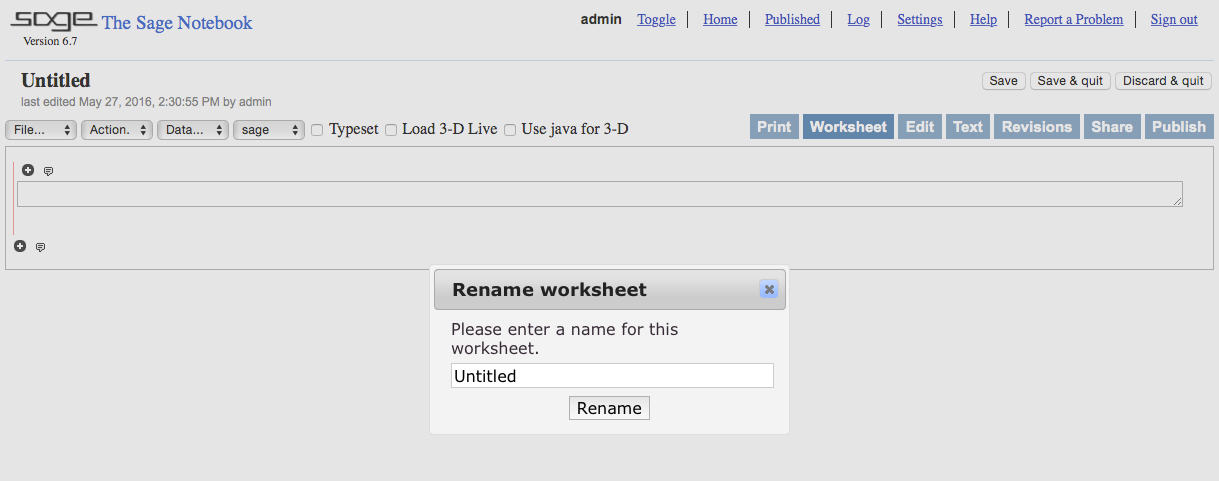
\includegraphics[width=0.8\columnwidth]{graphics/screenshots/StartingWorksheetModeOwnServer}\tabularnewline
Independent server\tabularnewline
\hline 
\end{tabular}
\par\end{center}

\begin{center}
\begin{tabular}{|c|}
\hline 
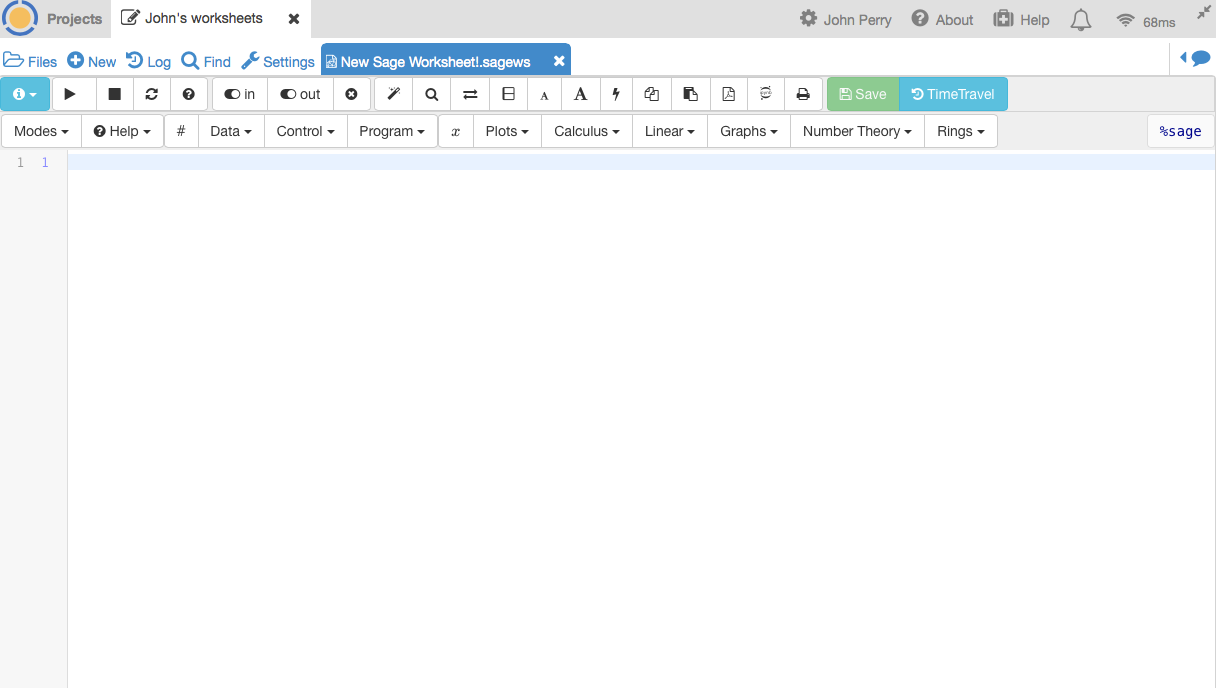
\includegraphics[width=0.8\columnwidth]{graphics/screenshots/StartingWorksheetModeCoCalc}\tabularnewline
CoCalc\tabularnewline
\hline 
\end{tabular}
\par\end{center}

\noindent You can (and should) change the title.
\begin{itemize}
\item In the independent server, you can do that at the beginning with the
``Rename worksheet'' dialog you see in the screenshot. You can do
it later by clicking on the title (in the upper left, currently ``Untitled'')
and the same dialog will pop up.
\item In CoCalc, you can do that by clicking on the circled \keyboardpress{i}
in the upper left and choosing ``Rename\ldots ''. A new screen
will appear, prompting you to rename the file. Make sure you keep
the \keyboardpress{.sagews} added at the end.
\end{itemize}
There are other options you can monkey with, but for now we'd recommend
you move on to the next chapter, since most of those options are of
small importance for our purposes. The ones we do need we'll discuss
in due course.

\subsection*{Command-line Sage}

If you choose to run Sage from the command line, you need to open
a \emph{shell}, also called \emph{a command-line prompt}. You will
see some sort of prompt, which can vary quite a bit; whenever we mean
a shell prompt we'll simply put a blue greater-than symbol: \textcolor{blue}{\keyboardpress{\textcolor{blue}{>}}}.
At the prompt, type \keyboardpress{sage}, press \keyboardpress{Enter},
then wait for Sage to start up. This might take a few seconds, but
eventually you will see something to this effect:
\begin{sageinteraction}
\texttt{\textcolor{blue}{>}}\texttt{ sage}

\noindent\fbox{\begin{minipage}[t]{1\columnwidth - 2\fboxsep - 2\fboxrule}%
\texttt{SageMath Version 6.7, Release Date: 2015-05-17}

\texttt{Type \textquotedbl notebook()\textquotedbl{} for the browser-based
notebook interface.}

\texttt{Type \textquotedbl help()\textquotedbl{} for help.}%
\end{minipage}}

\texttt{\textcolor{blue}{sage:}}\texttt{ \_}
\end{sageinteraction}

\noindent The underscore (\keyboardpress{\_}) might actually look
like a little box on your system. Once you see that, you're in good
shape for the next chapter. If you \emph{don't} see it, or if you
see some sort of error, you need to talk with your instructor or tech
support and see what went wrong.

If you'd like to run a Sage worksheet in a browser, but don't want
to run CoCalc and don't have access to another server, type \keyboardpress{notebook()}
and press \keyboardpress{Enter}. You will see a lot of messages,
for instance:
\begin{sageinteraction}
\texttt{\textcolor{blue}{sage:}}\texttt{ notebook()}

\texttt{The notebook files are stored in: sage\_notebook.sagenb}

\noindent\fbox{\begin{minipage}[t]{1\columnwidth - 2\fboxsep - 2\fboxrule}%
\texttt{Open your web browser to http://localhost:8080}%
\end{minipage}}

\texttt{Executing twistd -{}-pidfile=\textquotedbl sage\_notebook.sagenb/sagenb.pid\textquotedbl{}
-ny \textquotedbl sage\_notebook.sagenb/twistedconf.tac\textquotedbl}

\texttt{/Applications/sage-6.7-untouched/local/lib/python2.7/site-packages/}

\texttt{Crypto/Util/number.py:57: PowmInsecureWarning: Not using mpz\_powm\_sec. You
should rebuild using libgmp >= 5 to avoid timing attack vulnerability.}

\texttt{\_warn(\textquotedbl Not using mpz\_powm\_sec. You should
rebuild using libgmp >= 5 to avoid timing attack vulnerability.\textquotedbl ,
PowmInsecureWarning)}

\texttt{2016-05-27 14:30:49+0300 {[}-{]} Log opened.}

\texttt{2016-05-27 14:30:49+0300 {[}-{]} twistd 14.0.2 (/Applications/sage-6.7-untouched/local/bin/python
2.7.8) starting up.}

\texttt{2016-05-27 14:30:49+0300 {[}-{]} reactor class: twisted.internet.selectreactor.SelectReactor.}

\texttt{2016-05-27 14:30:49+0300 {[}-{]} QuietSite starting on 8080
2016-05-27 14:30:49+0300 {[}-{]} Starting factory <\_\_builtin\_\_.QuietSite
instance at 0x1181bb638>}
\end{sageinteraction}

\noindent For the most part, you \emph{do not} need to worry about
those messages.\footnote{Well, maybe the security warnings about \keyboardpress{libgmp}, if
you see them. I should look into that.} You don't even have to follow the directions to open your web browser
to that site; on many machines, the browser will open the webpage
automatically. Besides, it will take a few seconds for things to get
started, so sit back and relax a few seconds. If your browser doesn't
open, Don't Panic! Open it yourself and see if the web address \emph{your}
Sage advises works. If it does, you're in good shape for the next
chapter.

If it doesn't,\index{PANIC@\textcolor{red}{PANIC"!}}
\begin{center}
\textcolor{red}{\LARGE{}PANIC!}{\LARGE\par}
\par\end{center}

\noindent Yes, it really is okay to panic once in a while. Get it
out of your system. Once you're done, look carefully at the messages,
and see if any are error messages; these would be helpful. Then visit
\begin{center}
\keyboardpress{\href{https://groups.google.com/forum/\#!forum/sage-support}{https://groups.google.com/forum/\#!forum/sage-support}}
\par\end{center}

\noindent and search to see if that error message has been discussed.
If not, start a new post, inquiring about what's going wrong.

\section*{Getting help}

If you're reading this as part of a class, then your instructor should
be helpful. (Maybe not \emph{very} helpful, but helpful all the same.)
We already mentioned the \keyboardpress{sage-support} forum last
chapter. Aside from these options, Sage will answer many questions
on its own.

\subsection*{Docstrings}

If you want to know how a command works, type the name of the command,
followed by a question mark, then execute the command. Sage will provide
you useful information on the command, typically with examples.
\begin{sageinteraction}

\sageinput{simplify?}

\sageoutput{\textcolor{red}{Signature:} simplify(f)}

\sageoutput{\textcolor{red}{Docstring:}}

\sageoutput{~~~~Simplify the expression f.}

\sageoutput{~}

\sageoutput{~~~~EXAMPLES: We simplify the expression i + x - x.}

\sageoutput{~}

\sageoutput{~~~~~~~~sage: f = I + x - x; simplify(f)}

\sageoutput{~~~~~~~~I}

\sageoutput{In fact, printing f yields the same thing - i.e., the simplified
form.}

\sageoutput{\textcolor{red}{Init docstring:} x.\_\_init\_\_(...) initializes
x; see help(type(x)) for signature}

\sageoutput{\textcolor{red}{File:} /Applications/sage-6.7-untouched/local/lib/python2.7/site-}

\sageoutput{packages/sage/calculus/functional.py}

\sageoutput{\textcolor{red}{Type:} function}
\end{sageinteraction}


\subsection*{Finding methods for objects}

Another way to get help is to see what commands an object will accept
as \emph{methods}. A ``method\index{message!error message|see{the particular error}}\index{class!method}\index{method|see {class method}}''
is a command that is very specific to a particular Sage object; you
invoke it by typing the object's name, followed by a dot, then the
name of the method.\footnote{Another term for ``method'' is ``message;'' both terms are used
in computer science, but ``method'' is the jargon for Sage.} To find the names of all the methods an object accepts, type its
name, followed by a dot, then press the \keyboardpress{Tab} key.\index{tab completion}

For example, \sageword{simplify()} doesn't work very well on the
following expression:\footnote{It does actually work in some versions of Sage, such as Sage 6.7,
but not in others, such as 8.1. If it simplifies in your version,
just pretend that it doesn't for the sake of the argument, and follow
along, since that isn't the point anyway.}
\begin{sageinteraction}

\sageinput{rats = 1/x + 1/2}

\sageinput{simplify(rats)}

\sageoutput{1/x + 1/2}

\end{sageinteraction}

\noindent We \emph{really} want to simplify that expression as fully
as possible, so let's see if it accepts a method that will perform
a more thorough simplification. Type \sageword{rats.} (including
the period!) and then press \keyboardpress{Tab}; you should see over
200 possible methods. Some of them are not really appropriate for
the expression; we won't go into the reasons for this, but if you
look carefully, you should find at least two useful methods. One of
them is \sageword{full\_simplify()}.
\begin{sageinteraction}

\sageinput{rats.full\_simplify()}

\sageoutput{1/2{*}(x + 2)/x}

\end{sageinteraction}

\noindent That's a somewhat convoluted way of writing $\nicefrac{\left(x+2\right)}{\left(2x\right)}$,
but at least it's simplified!

The thought of hunting through over 200 possible methods may seem
intimidating, but many objects accept very few methods. In practice,
this isn't such a difficult technique, since there are many ways to
search through the list.

\section*{Exercises}

\subsection*{True/False. If the statement is false, replace it with a true statement.}
\begin{lyxlist}{99.}
\item [{1.}] This is just another programming textbook.
\item [{2.}] Mathematics is about counting numbers.
\item [{3.}] While students don't much care for fractions, computers find
it easier to work with fractions than with floating point numbers.
\item [{4.}] ``Free'' software is written by unemployed slackers living
in their parents' basements.
\item [{5.}] All famous mathematical results were appreciated from the
start for their clear, elegant proofs.
\item [{6.}] Bytecode is technically not an interpreted language.
\item [{7.}] Interpreted languages are appreciated above all else for their
speed.
\item [{8.}] Some software of significant size is bug-free.
\item [{9.}] Abstract mathematics is useless in the real world.
\item [{10.}] It is easy to verify and improve on proprietary mathematics
packages.
\item [{11.}] \emph{Bonus:} The answer to all these True/False questions
is ``False.''
\end{lyxlist}

\subsection*{Multiple Choice}
\begin{lyxlist}{99.}
\item [{1.}] Which of the following is \emph{not} an example of a computer
algebra system?
\begin{lyxlist}{M.}
\item [{A.}] A package that performs fraction arithmetic without any roundoff
error at all.
\item [{B.}] A package that assigns numbers to musical notes and uses fractals
to produce new music.
\item [{C.}] A package that performs polynomial arithmetic with approximate
values for coefficients.
\item [{D.}] A package that focuses on sets of abstract objects defined
by precise properties.
\end{lyxlist}
\item [{2.}] Which of the following is \emph{not} a step in the usual process
of compiling a program?
\begin{lyxlist}{M.}
\item [{A.}] The compiler reads the source from a file.
\item [{B.}] The compiler translates each symbol into a combination of
\textbf{on} and \textbf{off} signals.
\item [{C.}] The compiler saves the translation to a file, called an executable
or a library.
\item [{D.}] The compiler executes the translated commands immediately
before quitting.
\end{lyxlist}
\item [{3.}] Sage's primary focus is what kind of computational mathematics?
\begin{lyxlist}{M.}
\item [{A.}] numerical computation with approximate values
\item [{B.}] statistical computation with probable values
\item [{C.}] symbolic computation with exact values
\item [{D.}] fuzzy computation with uncertain values
\end{lyxlist}
\item [{4.}] Which of the following computer algebra systems would you
use to compute a derivative?
\begin{lyxlist}{M.}
\item [{A.}] Maxima
\item [{B.}] PARI
\item [{C.}] Schoonship
\item [{D.}] \textsc{Singular}
\end{lyxlist}
\item [{5.}] Which of the following well-known computer languages tries
to straddle the gap between interpreted and compiled languages?
\begin{lyxlist}{M.}
\item [{A.}] C/C++
\item [{B.}] Fortran
\item [{C.}] Java
\item [{D.}] Python
\end{lyxlist}
\item [{6.}] Which of the following is a primary motivation of the movement
for ``free'' mathematics software?
\begin{lyxlist}{M.}
\item [{A.}] Antipathy to censorship
\item [{B.}] International collaboration
\item [{C.}] Lack of grant funding
\item [{D.}] Verifiability of results
\end{lyxlist}
\item [{7.}] Which of the following mathematicians is famous in spite of
popularizing a ``fact'' that was very wrong?
\begin{lyxlist}{M.}
\item [{A.}] Pierre de Fermat
\item [{B.}] Marin Mersenne
\item [{C.}] William Stein
\item [{D.}] Andrew Wiles
\end{lyxlist}
\item [{8.}] Which of the following mathematicians is famous in spite of
his non-scientific day job?
\begin{lyxlist}{M.}
\item [{A.}] Pierre de Fermat
\item [{B.}] Marin Mersenne
\item [{C.}] William Stein
\item [{D.}] Andrew Wiles
\end{lyxlist}
\item [{9.}] Which of the following is \emph{not} an advantage to working
with Sage?
\begin{lyxlist}{M.}
\item [{A.}] You acquire practical skills that employers value.
\item [{B.}] You work with cutting-edge software.
\item [{C.}] You no longer have to worry about getting the correct answer.
\item [{D.}] You can use the material learned here in other classes.
\end{lyxlist}
\item [{10.}] In which of these ways does Sage work with Python?
\begin{lyxlist}{M.}
\item [{A.}] Sage's interface is essentially a Python interface.
\item [{B.}] Sage is a Python library you can load into any Python interpreter.
\item [{C.}] Python is one of the computer algebra systems in Sage.
\item [{D.}] Sage uses the Cython compiler to compile all Python programs.
\end{lyxlist}
\item [{\emph{Bonus:}}] Which answer is correct?
\begin{lyxlist}{M.}
\item [{A.}] The next one.
\item [{B.}] The next one.
\item [{C.}] The next one.
\item [{D.}] The first one.
\end{lyxlist}
\end{lyxlist}

\subsection*{Short answer}
\begin{lyxlist}{9.}
\item [{1.}] Explain how the quote at the beginning of this chapter is
related to its main thesis.
\item [{2.}] Describe a real-world analogy for the difference between compiled,
interpreted, and bytecode languages.
\item [{3.}] A common problem in mathematics textbooks is to compute the
1001st derivative of $\cos x$. The best way to find the answer is
\emph{not} to compute all~1001 derivatives; instead, you compute
a few, notice a pattern, and deduce quickly what the 1001st derivative
should be. Explain how this compares to what we want you to get out
of this text.
\item [{4.}] Not all mathematicians find the arguments in favor of free
software convincing, and the use of proprietary software is widespread.
Why do you think this is the case?
\item [{5.}] Even if Sage is less popular than a proprietary package like
Maple or Mathematica, learning Sage can make it easier to work with
those packages, as well. Why?
\end{lyxlist}

\chapter{Basic computations}
\begin{quotation}
What's in a name? that which we call a rose / By any other name would
smell as sweet\ldots{} (Shakespeare)
\end{quotation}
\label{chap: basic computations}Create a new worksheet and call it
``My First Sage Worksheet.''

To describe interaction with Sage, we use the following format:
\begin{sageinteraction}

\sageinput{some input}

\sageoutput{some output}

\end{sageinteraction}

\noindent The text ``\sageword{some input}'' indicates a command
you type into Sage. If you are using Sage from the command line, you
will type this at a blue ``\texttt{\textcolor{blue}{sage:}}'' prompt;
hence the blue color and the label. If you are using Sage from a worksheet,
you will not see a prompt; instead, you will type the command in a
``cell,'' which in some versions of Sage is outlined by a small
box.

To execute the command:
\begin{itemize}
\item at the command line, press the \keyboardpress{Enter} or \keyboardpress{Return}
key;
\item in a worksheet, hold \keyboardpress{Shift} and press the \keyboardpress{Enter}
or \keyboardpress{Return} key.
\end{itemize}
Sage will then interpret and process your command. The worksheet interface
will show a colored or flashing bar while Sage does this; the command-line
interface will simply pause.

Once the output is complete, you will see the text indicated by ``\textcolor{blue}{\sageword{\textcolor{blue}{some output}}}.''
If the command succeeded, you will see an answer that looks more or
less sensible. If an error occurred, the text will include a lot of
information, some of it in \texttt{{\color{sageerrorcolor}}red\texttt{}}
(the last line especially, which is all we will copy) and probably
won't make sense unless you already know Python. For instance:
\begin{sageinteraction}

\sageinput{some bad input}

\sageerror{SomeError: some message to explain the error}

\end{sageinteraction}

\noindent We will explain several types of errors as we progress through
our explorations of Sage. As a convenience, we are adding errors to
the textbook's index. If you are working on some computation, and
you run across some error you don't recognize, see if you can find
it in the index; if so, the page numbers it references will prove
helpful.

Here's an example of a successful computation; you should try this
yourself now and make sure you get the same result.
\begin{sageinteraction}

\sageinput{2 + 3}

\sageoutput{5}

\end{sageinteraction}

\noindent That looks reassuring; at least Sage can do that! Here's
one where the user forgot to let go of the \keyboardpress{Shift}
key before pressing the number 3.
\begin{sageinteraction}

\sageinput{2 + \#}

\sageerror{SyntaxError: invalid syntax}

\end{sageinteraction}

\noindent If you actually run this in Sage,\index{SyntaxError@\sageconstant{SyntaxError}!invalid syntax@\sageword{invalid syntax}}
you'll notice there's a bit more text in the error, as well as a lot
of color changes. In our case, this turns out to look like:
\begin{sageinteraction}

\texttt{{\color{softblue}File {\color{softgreen}\textquotedbl <ipython-input-3-7c2c726856a7>\textquotedbl},
line} {\color{softgreen}1}}

\texttt{~~{\color{sageerrorcolor}Integer(2) + \#}}

\texttt{~~~~~~~~~~~~~~~~\textasciicircum}

\texttt{{\color{sageerrorcolor}SyntaxError: invalid syntax}}
\end{sageinteraction}

\noindent You'll notice we \emph{only} copied the last line, which
specifies the type of error! When necessary for the discussion, we'll
sometimes include the rest of the information as well, but you can
often figure out the problem just from looking at the last line.

It may happen that the line you have to type is too long to fit in
one line. It \emph{will} happen to the authors of this text, since
we don't have that much horizontal space on the page. In cases like
this, you can keep typing, which can make the code harder to read,
or you can tell Sage you want to continue on the following line by
typing a backslash \sageword{\textbackslash}, which Sage interprets
as ``line break\index{line break},'' then pressing \keyboardpress{Enter}.
We will do this rather regularly to help make code more readable.
There is no need to wait until we bump up to the end of the line for
this, and sometimes it may be more readable to add the line break
early. For instance:
\begin{sageinteraction}

\sageinput{1 + 2 + 3 + 4 + 5 + 6 + 7 + 8 + 9 + 10 \textbackslash}

\noindent \texttt{....:~~~+ 11 + 12 + 13 + 14 + 15}

\sageoutput{120}
\end{sageinteraction}


\paragraph*{(When using a Sage worksheet)}

\label{par: HTML cells}One advantage to using Sage worksheets is
that you can use HTML commands to add explanatory narrative to your
work. Simply type
\begin{sageinteraction}

\sageinput{\%html}

\end{sageinteraction}

\noindent \ldots and everything following that line will be considered
HTML text. The toolbar will change to allow for HTML formatting, but
if you are familiar with HTML tags then you can add them directly.
You can format it the same way as you execute a Sage command: hold
\keyboardpress{Shift}, press \keyboardpress{Enter}. If needed, you
can then edit the HTML cell again by double-clicking on it. This is
enormously useful when breaking up a long worksheet into sections,
with headers that organize related parts of the work.

\section*{Yer basic arithmetic}

As you might expect, Sage offers the same basic arithmetic operations
you can find in any calculator. Here are a few that will prove useful.\footnote{You can also type $a$\sageword{\textasciicircum}$b$ for exponentiation,
but for various reasons we don't recommend it: in some situations,
Sage will interpret it as a different operator.}
\begin{center}
\begin{table}[H]
\begin{centering}
\begin{tabular}{|c|l|}
\hline 
$a$\sageword{+}$b$ & adds $a$ and $b$\tabularnewline
\hline 
$a$\sageword{-}$b$ & subtracts $a$ and $b$\tabularnewline
\hline 
$a$\sageword{{*}}$b$ & multiplies $a$ and $b$\tabularnewline
\hline 
$a$\sageword{/}$b$ & finds the ratio of dividing $a$ by $b$\index{division!ratio, quotient, and remainder}\tabularnewline
\hline 
$a$ \sageword{//} $b$ & finds the quotient\index{quotient} of dividing $a$ by $b$\tabularnewline
\hline 
$a$\sageword{\%}$b$ & finds the remainder\index{remainder} of dividing $a$ by $b$\tabularnewline
\hline 
$a$\sageword{{*}{*}}$b$ & raises $a$ to the $b$th power\index{power}\index{exponentiation}\tabularnewline
\hline 
\sageword{sqrt(}$a$\sageword{)} & the \index{square root}square root of $a$\tabularnewline
\hline 
\sageword{abs(}$a$\sageword{)} & the \index{absolute value}absolute value of $a$\tabularnewline
\hline 
\end{tabular}
\par\end{centering}
\caption{Sage operators for basic arithmetic}
\end{table}
\par\end{center}

\noindent Go ahead and try these with some numbers, both approximate
and exact.

\subsection*{Yer basic comparisons}

Sage can also compare objects, to a certain extent.
\begin{table}[H]
\begin{centering}
\begin{tabular}{|c|l|}
\hline 
$a$\sageword{>}$b$ & is $a$ strictly greater than $b$?\tabularnewline
\hline 
$a$\sageword{>=}$b$ & is $a$ greater than or equal to $b$?\tabularnewline
\hline 
$a$\sageword{==}$b$ & is $a$ equal to $b$?\tabularnewline
\hline 
$a$\sageword{<=}$b$ & is $a$ less than or equal to $b$?\tabularnewline
\hline 
$a$\sageword{<}$b$ & is $a$ strictly less than $b$\tabularnewline
\hline 
\end{tabular}
\par\end{centering}
\caption{Sage operators for basic comparisons}
\end{table}

\noindent When using these comparisons, Sage will return \sageconstant{True}\index{True@\sageconstant{True}}
or \sageconstant{False}\index{False@\sageconstant{False}}, which
obviously correspond to ``yes'' or ``no.''
\begin{sageinteraction}

\sageinput{2 < 3}

\sageoutput{True}

\sageinput{2 > 3}

\sageoutput{False}

\end{sageinteraction}

\noindent You have to be careful with comparison of equality, as the
sign is doubled. Problems will arise if you forget it.
\begin{sageinteraction}

\sageinput{2 = 3}

\sageerror{ValueError: The name \textquotedbl 2\textquotedbl{} is not a valid
Python identifier.}

\end{sageinteraction}

\noindent If you see that error message,\index{ValueError@\sageconstant{ValueError}!The name@\sageword{The name \ldots{} is not a valid Python identifier}}
the problem is almost certainly due to the use of only one equals
sign when you need two.

Aside from comparing numbers, \emph{many} symbolic objects can be
compared. We won't talk about sets for quite some time, for instance,
but there is a natural ordering of sets based on subset properties,
and Sage will compare sets based on that fact. Consider, for instance,
the sets $\left\{ 2,3\right\} $, $\left\{ 2,4\right\} $, and $\left\{ 2,3,4,5\right\} $:
\begin{sageinteraction}

\sageinput{\{2,3\} < \{2,3,4,5\}}

\sageoutput{True}

\sageinput{\{2,3,4,5\} > \{2,3\}}

\sageoutput{True}

\sageinput{\{2,3\} < \{2,4\}}

\sageoutput{False}
\end{sageinteraction}


\subsection*{Exact v.~approximate values}

Sage offers symbols to represent the exact values of some important
numbers; these should be easy to remember.\footnote{It is also possible to use \sageconstant{i} for the imaginary number,
but as it is common to use \sageword{i} as a variable we try to avoid
that.}

\begin{table}[H]
\begin{centering}
\begin{tabular}{|c|l|}
\hline 
\index{pi@$\pi$}\index{pi@\sageconstant{pi}}\sageconstant{pi} & $\pi$, the ratio of a circle's circumference to its radius\tabularnewline
\hline 
\multirow{2}{*}{\index{e@\sageconstant{e}}\sageconstant{e}} & ${\displaystyle e=\lim_{x\rightarrow\infty}\left(1+\frac{1}{x}\right)^{x}}$,
\emph{or},\tabularnewline
 & the value of $a$ such that the derivative of $a^{x}$ is $a^{x}$\tabularnewline
\hline 
\index{I@\sageconstant{I}}\sageconstant{I} & $i$, the ``imaginary'' number ($i^{2}=-1$)\tabularnewline
\hline 
\index{oo@\sageconstant{oo}|see{infinity}}\sageconstant{oo}\emph{
or} & \multirow{2}{*}{$\infty$, infinity (unbounded above)}\tabularnewline
\index{infinity!+Infinity@\sageconstant{+Infinity}}\sageconstant{+Infinity} & \tabularnewline
\hline 
\index{oo@\sageconstant{-oo}|see{infinity}}\sageconstant{-oo}\emph{
or} & \multirow{2}{*}{$-\infty$ (unbounded below)}\tabularnewline
\sageconstant{-Infinity}\index{infinity!-Infinity@\sageword{-Infinity}} & \tabularnewline
\hline 
\end{tabular}
\par\end{centering}
\caption{Sage symbols for important constants}
\end{table}

\noindent We italicize these identifiers in the text, both to help
with readability and to highlight that they should represent fixed
values.\footnote{As we note on page~\pageref{note: sage "constants" not constant},
though, Sage does not have true constants, so a user or program can
change the symbols' meanings.} Sage does not italicize them in output.

We explained already that the strength of a computer algebra system
like Sage lies in its ability to manipulate exact values, rather than
approximate values. Nevertheless, we sometimes need to compute with
approximate values, and Sage allows this as well.
\begin{center}
\textbf{\emph{To use approximate arithmetic, type at least one number
as a decimal!}}
\par\end{center}

\noindent To see how it works, consider the following commands and
their results.
\begin{sageinteraction}

\sageinput{2/3}

\sageoutput{2/3}

\sageinput{2./3}

\sageoutput{0.666666666666667}

\end{sageinteraction}

\noindent In the first case, you entered exact values, so Sage gives
you the \emph{exact} quotient of dividing 2 by 3, the fraction $\nicefrac{2}{3}$.
In the second case, you're specifying at least one decimal, so you're
getting the \emph{approximate} quotient of dividing 2 by 3. This may
look like floating-point, but it's not quite; it's actually an object
Sage calls a \sageword{RealNumber}. Don't worry about those details
right now.

\section*{Constants, variables, and indeterminates}

\subsection*{A subtle distinction in usage}

The mathematical symbols $e$, $\pi$, and $i$ represent \emph{constants,}
by which we mean their values are definite and fixed. If someone writes
Euler's equation,
\[
e^{i\pi}+1=0,
\]
then every educated mathematician will know the values of $e$, $i$,
and $\pi$, even if this is the first time they see the equation.
Thanks to the symbols we described above, this holds true in Sage,
as well:
\begin{sageinteraction}

\sageinput{e{*}{*}(I{*}pi) + 1}

\sageoutput{0}

\end{sageinteraction}

\noindent Of course, there are times when any of these symbols can
mean something else. For instance, $x_{i}$ refers to the $i$th number
in a list, not to some manipulation of $x$ by the imaginary number.

Other one-letter symbols in mathematics represent one of two kinds
of \emph{variables,} by which we mean their values are not necessarily
fixed during a problem. The symbol $x$, for instance, can represent
any of an infinite number of values. Mathematicians generally work
with two kinds of variables; and in ordinary parlance, we tend to
refer to both kinds as variable, but in fact there is an important
distinction, which we can see in an expression as simple as the polynomial
\[
x^{2}-c^{2}.
\]

\begin{itemize}
\item In many situations, specific values for $x$ and $c$ are very important.
The equation
\[
x^{2}-c^{2}=2
\]
is not always true; it depends on the values of $x$ and $c$, and
in practice we often try to find values for which this is true.
\item In other situations, however, $x$ and $c$ represent arbitrary values.
The equation
\[
x^{2}-c^{2}=\left(x+c\right)\left(x-c\right)
\]
is true regardless of the values of $x$ and $c$.
\end{itemize}
This matters a great deal for computer algebra systems, because a
symbol can likewise refer to a specific or indeterminate value, and
we need to pay attention to this distinction from time to time. We
will agree on the following convention:
\begin{itemize}
\item When a symbol has been assigned a specific value, we usually call
it a \emph{variable\index{variable},} because we can change that
value at any time.
\item When \emph{we have no intention} of changing a variable's value, we
call it a \emph{constant}\index{constant}.
\item When a symbol is not to hold any specific value, but is purely symbolic
for an arbitrary value from some set, we call it \emph{indeterminate}\index{indeterminate}.
\end{itemize}
Sage provides only one indeterminate at startup: \sageword{x}. If
you want to work with another indeterminate, such as \sageword{y},
you have to create it.

\label{note: sage "constants" not constant}Sage does not offer a
way to define your own constants, the way some programming languages
do. In Sage, a constant is just a variable that you try really hard
not to change.

\subsection*{Resetting a variable or indeterminate}

Since Sage has no way for you to define true constants, you can, if
you choose, reassign the value of \sageconstant{I} to something else,
and it is very likely that you will do that someday, in some circumstance.
If that happens, it is easy to fix with the \sageword{reset()}\index{reset@\sageword{reset()}}\index{variable!resetting a name}\index{indeterminate!resetting a name}
command; include the symbol between quotes inside the parentheses.
\begin{sageinteraction}

\sageinput{I\textasciicircum 2 + 1}

\sageoutput{0}

\sageinput{I = 2}

\sageinput{I\textasciicircum 2 + 1}

\sageoutput{5}

\sageinput{reset('I')}

\sageinput{I\textasciicircum 2 + 1}

\sageoutput{0}
\end{sageinteraction}


\subsection*{Creating variables and indeterminates}

To create a variable, use the assignment construct,
\begin{center}
\emph{identifier }\sageword{=}\emph{ expression}
\par\end{center}

\noindent where \emph{identifier\index{identifier}} is a legitimate
name for an identifier of a symbol and \emph{expression} is a legitimate
mathematical expression. For instance,
\begin{sageinteraction}

\sageinput{sqrt2 = sqrt(2)}

\end{sageinteraction}

\noindent assigns the value of $\sqrt{2}$ to the symbol \sageword{sqrt2}.
After making this assignment, you can use the symbol \sageword{sqrt2}
in any expression, and Sage will see it as $\sqrt{2}$. For example:
\begin{sageinteraction}

\sageinput{sqrt2{*}{*}2}

\sageoutput{2}

\end{sageinteraction}

Unlike programming languages that allow you to assign to only one
variable at a time, Sage inherits Python's more flexible assignment,
which allows you to assign to many variables in one go. For example,
\begin{sageinteraction}

\sageinput{sqrt2, sqrt3 = sqrt(2), sqrt(3)\label{assignment to multiple variables}}

\sageinput{sqrt2{*}{*}2}

\sageoutput{2}

\sageinput{sqrt3{*}{*}4}

\sageoutput{9}

\end{sageinteraction}

\noindent The first line in this sequence of statements assigns \emph{both}
$\sqrt{2}$ and $\sqrt{3}$ to the variables \sageword{sqrt2} and
\sageword{sqrt3}, \emph{in that order.} The two subsequent statements
show that the assignments were indeed correct. Because of this, you
can probably see that the statement
\begin{sageinteraction}

\sageinput{sqrt2, sqrt3 = sqrt3, sqrt2}

\end{sageinteraction}

\noindent has the effect of swapping the values of \sageword{sqrt2}
and \sageword{sqrt3}.

To create an indeterminate, Sage provides a command, \sageword{var()}.
Type the name you'd like the indeterminate to have between the parentheses,
\emph{in quotes}. You can create several such indeterminates by listing
them between the quotes, as well; just leave a space between each
name. If successful, Sage will print the names of the newly created
indeterminates between parentheses. For example:
\begin{sageinteraction}

\sageinput{var('y z')}

\sageoutput{(y, z)}

\end{sageinteraction}

\noindent You can then manipulate these variables to your heart's
content.
\begin{sageinteraction}

\sageinput{(y + z) + (z - y)}

\sageoutput{2{*}z}
\end{sageinteraction}


\subsection*{Valid identifiers}

\label{subsec:valid identifier names}Each variable or indeterminate
needs a valid identifier. Sage accepts identifier names using the
following sequences of characters:
\begin{itemize}
\item The name must start with a letter (uppercase or lowercase) or the
underscore (\texttt{\sageword{\_}}).
\item The name can contain any mix of letters, numbers, or the underscore.
\item The name cannot be a \emph{reserved word,} also called a \emph{keyword}\index{keyword}.
You'll encounter these throughout the course, but it's unlikely you'd
choose them.
\end{itemize}
Unlike mathematical convention, the names of variables and indeterminates
can be longer than one symbol; we see this already in \sageword{pi},
which Sage offers at the start. In many cases, a name that is longer
than one symbol can be understood much more readily than a name that
is only one symbol; compare, for instance, \sageword{d} to \sageword{derivative}.
On the other hand, if a name is \emph{too} long and you use it repeatedly,
it grows tiresome to type and can even make a program \emph{harder}
to understand. A mathematically literate person, for instance, would
understand \sageword{ddx} just as well as \sageword{derivative},
and might well prefer the former to the latter. In general, we'd recommend
no more than six characters in a name, though if a longer name is
helpful for clarity you can disregard this guideline, and should,
just as we will.

\section*{Expressions, and commands to manipulate them}

\label{page: begin factor, expand, etc.}A mathematical expression\index{expression!as distinct from equation}
consists of any meaningful combination of mathematical symbols. One
such expression is an \emph{equation}\index{equation}, and in Sage
you can assign equations as the values of variables. You definitely
need to do this from time to time, but the equals sign already has
a meaning: it assigns the value of an expression to a symbol to create
a variable! To refer to an equation, then, you use two equals signs
in a row:
\begin{sageinteraction}

\sageinput{eq = x{*}{*}2 - 3 == 1}

\end{sageinteraction}

\noindent As before, if you forget to double the equals signs, Sage
will give you an error:
\begin{sageinteraction}

\sageinput{eq = x{*}{*}2 - 3 = 1}

\sageerror{SyntaxError: can't assign to operator}

\end{sageinteraction}

\noindent We remind the reader that if you see that error message,\index{SyntaxError@\sageconstant{SyntaxError}!can't assign to operator@\sageword{can't assign to operator}}\index{equation!requires two equals signs}
the problem is almost certainly due to the use of only one equals
sign when you need two.

It is often useful to rewrite expressions in different ways, and a
computer algebra system is, essentially, nothing more than a sophisticated
tool for rewriting expressions. Here are some useful commands for
rewriting expressions.

\begin{table}[H]
\begin{centering}
\begin{tabular}{|c|l|}
\hline 
\index{factor@\sageword{factor()}}\sageword{factor(}\emph{exp}\sageword{)} & factor the expression \emph{exp}\tabularnewline
\hline 
\index{simplify@\sageword{simplify()}}\sageword{simplify(}\emph{exp}\sageword{)} & simplify the expression \emph{exp} a little bit\tabularnewline
\hline 
\index{expand@\sageword{expand()}}\sageword{expand(}\emph{exp}\sageword{)} & perform multiplication and other operations on the expression \emph{exp}\tabularnewline
\hline 
\index{round@\sageword{round()}}\sageword{round(}\emph{exp}\sageword{,}$n$\sageword{)} & round the expression \emph{exp} to $n$ places after the decimal\tabularnewline
\hline 
\end{tabular}
\par\end{centering}
\caption{\emph{Some} commands to manipulate expressions (there are a lot more)\label{page: expand()}}
\end{table}


\subsection*{Some words to the wise}

The traditional mathematical symbol for multiplication\index{multiplication|seealso{\sageword{expand()}}}\index{multiplication}
is the simple $\times$ or the dot symbol $\cdot$. Alas, computer
keyboards have neither symbol by default; you generally have to use
a workaround if you want to type the symbol. The traditional workaround
is to type the asterisk, and that is what Sage uses.

It is common in mathematics to omit the multiplication symbol: $2x$,
for instance, or $abcd$. You can't do this in Sage; that will give
you various errors:\index{SyntaxError@\sageconstant{SyntaxError}!invalid syntax@\sageword{invalid syntax}}\index{NameError@\sageconstant{NameError}!name is not defined@\sageword{name \ldots{} is not defined}}
\begin{sageinteraction}

\sageinput{2x}

\sageerror{SyntaxError: invalid syntax}

\sageinput{var('a b c d')}

\sageoutput{(a, b, c, d)}

\sageinput{abcd}

\sageerror{NameError: name 'abcd' is not defined}

\end{sageinteraction}

\noindent In both cases, Sage thinks you're trying to type the name
of an identifier, which name it doesn't recognize:
\begin{itemize}
\item For \sageword{2x}, you cannot start an identifier name with a number
so the error is in syntax.
\item For \sageword{abcd}, Sage has no practical way of knowing that you
mean the products of \sageword{a}, \sageword{b}, \sageword{c},
and \sageword{d}, rather than a different identifier named \sageword{abcd},
so the error is in fact one of the name. (Remember that in Sage, unlike
most mathematics, variables and indeterminates can have names longer
than one symbol.)
\end{itemize}
\noindent Both of these expressions work fine if you type the multiplication
symbol where you want it to be.\footnote{In some versions of Sage there is a way to make multiplication work
without explicitly writing the multiplication symbol in these circumstances,
but it is not available by default, so you'd have to run a special
command for it. This is a bad idea for beginners, and you'd still
have to type a space between the symbols in any case, so we will not
describe that technique.}\label{page: end factor, expand, etc.}

\subsection*{Transcendental functions}

Sage offers everything a scientific calculator offers. Here are some
common transcendental functions that you will find useful throughout
this text and in your math curriculum:
\begin{center}
\begin{table}[H]
\begin{centering}
\begin{tabular}{|c|l|}
\hline 
\sageword{sin(}$a$\sageword{)}, \sageword{cos(}$a$\sageword{)},
\sageword{tan(}$a$\sageword{)}, & the trigonometric functions,\tabularnewline
\sageword{cot(}$a$\sageword{)}, \sageword{sec(}$a$\sageword{)},
\sageword{csc(}$a$\sageword{)} & evaluated at $a$\tabularnewline
\hline 
\sageword{arcsin(}$a$\sageword{)}, \sageword{arccos(}$a$\sageword{)},
\sageword{arctan(}$a$\sageword{)}, & the inverse trigonometric functions,\tabularnewline
\sageword{arccot(}$a$\sageword{)}, \sageword{arcsec(}$a$\sageword{)},
\sageword{arccsc(}$a$\sageword{)} & evaluated at $a$\tabularnewline
\hline 
\sageword{exp(}$a$\sageword{)} & $e^{a}$ (synonym for \sageword{e{*}{*}a})\tabularnewline
\hline 
\sageword{ln(}$a$\sageword{)}, \sageword{log(}$a$\sageword{)} & the natural logarithm of $a$\tabularnewline
\hline 
\sageword{log\_b(}$a$\sageword{,} $b$\sageword{)} or \sageword{log(}$a$\sageword{,}$b$\sageword{)} & the logarithm base $b$ of $a$\tabularnewline
\hline 
\end{tabular}
\par\end{centering}
\caption{Sage commands for common transcendental functions}
\end{table}
\par\end{center}

\noindent We can also compute the hyperbolic trigonometric functions,
and their inverses, by appending \sageword{h} at the end of the usual
name, and before the left parenthesis.

You may have noticed that \sageword{log(}$a$\sageword{)} is synonymous
for \sageword{ln(}$a$\sageword{)}. This is not the usual custom
in American textbooks, where \sageword{log(}$a$\sageword{)} is
synonymous for $\log_{10}a$. To compute what Americans call the ``common''
logarithm, we have to use the \sageword{log\_b()} command:
\begin{sageinteraction}

\sageinput{log(100)}

\sageoutput{log(100)}

\sageinput{log\_b(100,10)}

\sageoutput{2}

\end{sageinteraction}

\noindent Be careful when trying to use these functions in larger
expressions. It is common in mathematics to write $\sin^{2}\nicefrac{\pi}{4}$
when you mean $\left(\sin\left(\nicefrac{\pi}{4}\right)\right)^{2}$.
Sage does not make this distinction. There is really only one way
to do it right, and that is to write\index{TypeError@\sageconstant{TypeError}!object is not callable@\sageword{\ldots object is not callable}}\index{TypeError@\sageconstant{TypeError}!unsupported operand type(s)@\sageword{unsupported operand type(s)}}
what you mean:
\begin{sageinteraction}

\sageinput{sin\textasciicircum 2(pi/4)}

\sageerror{TypeError: 'sage.rings.integer.Integer' object is not callable}

\sageinput{(sin\textasciicircum 2)(pi/4)}

\sageerror{TypeError: unsupported operand type(s) for {*}{*} or pow(): 'Function\_sin'
and 'int'}

\sageinput{(sin(pi/4))\textasciicircum 2}

\sageoutput{1/2}

\end{sageinteraction}

\noindent When you see \sageconstant{TypeError} with these messages,
it's a safe bet you've ``typed'' something wrong.\footnote{Technically, Sage is referring to the ``type'' of object, not to
what you've ``typed,'' but we're desperate enough to roll with the
pun.}
\begin{itemize}
\item The first kind of \sageword{TypeError} should be easy to debug: look
for a place where a number is followed immediately by the opening
of parentheses \textemdash{} in our case, \sageword{2(}\sageconstant{pi}\sageword{)/4}.
When this happens, Sage thinks you're trying to use \sageword{2}
as a function. The way Sage evaluates expressions, it sees $\sin^{2\left(\nicefrac{\pi}{4}\right)}$,
and while it might not seem sensible to us to view $2\left(\nicefrac{\pi}{4}\right)$
as a function $2$ evaluated at the point $\nicefrac{\pi}{4}$, that's
how Sage views it.
\item The second kind of \sageword{TypeError} can be harder. In general,
the problem is that you're trying to perform an operation with two
objects for which Sage doesn't know how to perform the operation.
Nine times out of ten, you've typed something wrong, so re-examine
what you've typed. In this case, you've typed a convenient shorthand,
which Sage doesn't understand (with reason).
\end{itemize}

\subsection*{Mathematical functions and substitution}

\index{substitution}A useful aspect of indeterminates is that you
can substitute values into them. Unlike assigning a value to a variable,
indeterminates don't retain that value after the computation. We use
three ways to substitute in Sage.

The first way is via the \sageword{subs()} method, which is shorthand
for the \sageword{substitute()} method. Recall that a \emph{method}
is a command that is specific to an object. You access this feature
in the following way:
\begin{itemize}
\item Type the expression's name, then a dot, then \sageword{subs(}~.
\item After the parenthesis, list the assignments. There are two ways to
do this:
\begin{itemize}
\item List each assignment as an equation: \emph{indeterminate}\sageword{=}\emph{value}.\footnote{This does not always work. We will return to the topic later.}
\item List each assignment as a ``dictionary\index{substitution!dictionary}''.
To do this, open a pair of braces, list the assignments in the form
\sageword{indeterminate:value}, separating each assignment by a comma,
then close the braces.
\end{itemize}
\item Now close the parentheses that began after \sageword{subs}: \sageword{subs(}\emph{assignments}\sageword{)}.
\end{itemize}
Here is an example:
\begin{sageinteraction}

\sageinput{f = x{*}{*}2}

\sageinput{f.subs(x=2)}

\sageoutput{4}

\sageinput{f.subs(\{x:2\})}

\sageoutput{4}

\end{sageinteraction}

\noindent The first substitution illustrates assignment via equations;
the second illustrates assignment via dictionaries. The second approach
is the most reliable, error- and warning-free way to substitute into
any mathematical expression that contains indeterminates.\footnote{In particular, the second approach works even inside user-defined
functions, also called a \emph{procedure}\index{procedure}, when
you want to pass an indeterminate as an argument to the procedure.
We talk about this later on.}

\index{substitution}A second way is to substitute without specifying
the method's name!
\begin{sageinteraction}

\sageinput{f(x=2)}

\sageoutput{4}

\sageinput{f(\{x:2\})}

\sageoutput{4}

\end{sageinteraction}

\noindent You \emph{should not} use this approach without specifying
the \emph{indeterminate's} name. If you have only one indeterminate,
as with \sageword{x} above, you may forget that you need to name
it. In this case, Sage will issue what's called a warning:
\begin{sageinteraction}

\sageinput{f(2)}

\sageerror{DeprecationWarning: Substitution using function-call syntax and unnamed
arguments is deprecated and will be removed from a future release
of Sage; you can use named arguments instead, like EXPR(x=..., y=...)}

\sageoutput{4}

\end{sageinteraction}

\noindent This warning\index{DeprecationWarning@\sageconstant{DeprecationWarning}!Substitution using function-call syntax@\sageword{Substitution using function-call syntax}}
might not appear on the last line. It's not an error, and Sage manages
to guess the correct substitution and outputs the correct answer after
the warning. In addition, a nice thing about \sageword{DeprecationWarning}s
is that they appear only once, even if you keep making the same ``mistake.''
All the same, it's a bit scary to see it there, and it's entirely
possible that the threat to remove this guess-and-go feature will
come to pass,\footnote{The warning has appeared for quite a few years now.}
so try not to make that mistake. This can be a real problem if you
provide too many values; Sage\index{ValueError@\sageconstant{ValueError}!the number of arguments@\sageword{the number of arguments}}
won't know what to assign where, and will complain:
\begin{sageinteraction}

\sageinput{f(3,2,1)}

\sageerror{ValueError: the number of arguments must be less than or equal to
1}

\end{sageinteraction}

\noindent This won't happen when you specify assignments, as Sage
knows what goes where:\index{substitution}
\begin{sageinteraction}

\sageinput{f = x\textasciicircum 2 - y\textasciicircum 2}

\sageinput{f(x=3,w=2,z=1)}

\sageoutput{-y\textasciicircum 2 + 9}

\end{sageinteraction}

The third way to substitute is useful when you're using a mathematical
expression called a \emph{function.} Recall that a function maps elements
of one set, called the \emph{domain,} to elements of another set,
called the \emph{range,} in such a way that every input has a well-defined
output. Defining and using functions is straightforward in Sage:
\begin{sageinteraction}

\sageinput{f(x) = x{*}{*}2}

\sageinput{f(2)}

\sageoutput{4}

\end{sageinteraction}

\noindent Functions also have the useful property that they define
any indeterminate that appears between the parentheses of their definition.
You can then use those indeterminates in other contexts without first
using the \sageword{var()} command.
\begin{sageinteraction}

\sageinput{f(w,z) = 4{*}w{*}{*}2 - 4{*}z{*}{*}2}

\sageinput{f(3,2)}

\sageoutput{20}

\sageinput{factor(w{*}{*}2 - z{*}{*}2)}

\sageoutput{(w + z){*}(w - z)}

\end{sageinteraction}

\noindent Notice that we were able to work with \sageword{w} and
\sageword{z} directly, even though we didn't define them.\index{substitution}

\section*{Yer basic Calculus}

We now turn to the question of Sage's offerings for the Calculus.

\subsection*{Exact computation}

We look at exact computation first. Sage offers three commands that
perform the exact computation for calculus.
\begin{table}
\begin{centering}
\begin{tabular}{|c|c|}
\hline 
\sageword{lim(}$f$\sageword{,}$x$\sageword{=}$a$\sageword{)} & \multirow{2}{*}{\index{lim@\sageword{lim}}\index{limit@\sageword{limit}}compute
the two-sided limit of $f\left(x\right)$ at $x=a$}\tabularnewline
\emph{or} \sageword{limit(}$f$\sageword{,}$x$\sageword{=}$a$\sageword{)} & \tabularnewline
\hline 
\sageword{lim(}$f$\sageword{,}$x$\sageword{=}$a$\sageword{, dir=}\emph{direction}\sageword{)} & compute the one-sided limit of $f\left(x\right)$ at $x=a$, with\tabularnewline
\emph{or} \sageword{limit(}$f$\sageword{,}$x$\sageword{=}$a$\sageword{, dir=}\emph{direction}\sageword{)} & \emph{direction} one of \sageword{'left'} or \sageword{'right'}\tabularnewline
\hline 
\sageword{diff(}$f$\sageword{,}$x$\sageword{)} & \index{derivative@\sageword{derivative}}\index{diff@\sageword{diff}}compute
the derivative of $f\left(x\right)$\tabularnewline
\emph{or} \sageword{derivative(}$f$\sageword{,}$x$\sageword{)} & with respect to $x$\tabularnewline
\hline 
\sageword{diff(}$f$\sageword{,}$x$\sageword{,}$m$\sageword{)} & compute the $m$th derivative\tabularnewline
\emph{or} \sageword{derivative(}$f$\sageword{,}$x$\sageword{,}$m$\sageword{)} & of $f\left(x\right)$ with respect to $x$\tabularnewline
\hline 
\sageword{integral(}$f$\sageword{,}$x$\sageword{)} & \index{integral@\sageword{integral}}\index{integrate@\sageword{integrate}}compute
the indefinite integral (antiderivative)\tabularnewline
\emph{or} \sageword{integrate(}$f$\sageword{,}$x$\sageword{)} & of $f\left(x\right)$ with respect to $x$\tabularnewline
\hline 
\sageword{integral(}$f$\sageword{,}$x$\sageword{,}$a$\sageword{,}$b$\sageword{)} & compute the definite integral over $\left[a,b\right]$\tabularnewline
\emph{or} \sageword{integrate(}$f$\sageword{,}$x$\sageword{,}$a$\sageword{,}$b$\sageword{)} & of $f\left(x\right)$ with respect to $x$\tabularnewline
\hline 
\end{tabular}
\par\end{centering}
\caption{\label{tab: exact calculus}Commands for exact computation of limits,
derivatives, and integrals}
\end{table}
 You can see in Table~\ref{tab: exact calculus} these commands,
with both synonyms and different usage options:
\begin{itemize}
\item For limits, we have the synonyms \sageword{lim()} and \sageword{limit()},
which we can use to compute either two-sided limits (default) or one-sided
limits (specify a direction). You must specify both the indeterminate
($x$) and the value ($a$).
\item For differentiation, we have the synonyms \sageword{diff()} and \sageword{derivative()},
which we can use either to differentiate once or, by specifying an
optional argument, to differentiate multiple times.
\item For integration, we have the synonyms \sageword{integral()} and \sageword{integrate()},
which we can use to compute either the indefinite integral, also called
the antiderivative, or if we specify the limits of integration, to
compute the definite integral, which you probably first learn as the
area under a function.
\end{itemize}
Let's take a quick look at how these work.

\subsubsection*{Limits}

First up is limits. Roughly speaking,
\begin{itemize}
\item ${\displaystyle \lim_{x\rightarrow a^{+}}f\left(x\right)}$ is the
$y$-value approached by $f$ as $x$ approaches $a$ from the right
(that is, from numbers larger than $a$);
\item ${\displaystyle \lim_{x\rightarrow a^{-}}f\left(x\right)}$ is the
$y$-value approached by $f$ as $x$ approaches $a$ from the left;
and
\item ${\displaystyle \lim_{x\rightarrow a}f\left(x\right)}$ is the $y$-value
approached by $f$ as $x$ approaches $a$ from both sides.
\end{itemize}
\noindent If a function is continuous at $a$, we can find the limit
by substitution, which is boring.
\begin{sageinteraction}

\sageinput{f(x) = x\textasciicircum 2 + 1}

\sageinput{limit(f(x), x=1)}

\sageoutput{2}

\sageinput{f(1)}

\sageoutput{2}

\end{sageinteraction}

\noindent Limits are much more interesting when the function is discontinuous
at $a$. Here are some problems you should remember from your Calculus
courses:
\begin{sageinteraction}

\sageinput{limit((x{*}{*}2 - 1)/(x - 1), x=1)}

\sageoutput{2}

\sageinput{limit(x/abs(x), x=0)}

\sageoutput{und}

\sageinput{limit(x/abs(x), x=0, dir='left')}

\sageoutput{-1}

\sageinput{limit(1/x, x=0, dir='left')}

\sageoutput{\sageconstant{-Infinity}}

\sageinput{limit(sin(1/x), x=0)}

\sageoutput{ind}

\end{sageinteraction}

\noindent What do these answers mean?
\begin{itemize}
\item The first example shows how Sage automatically detects and works around
division by zero, when possible.
\item The second example shows what can go wrong when there is no way to
work around it: \sageconstant{und}\index{und@\sageconstant{und}}
is shorthand for, ``the limit is undefined.'' In this case, there
are one-sided limits from left and right, and they are finite limits,
but they don't agree with each other.
\item The third and fourth examples show how to compute one-sided limits
in the case where two-sided limits do not exist.
\item In some cases, the limit doesn't exist because the function doesn't
approach any particular value. When this happens, but the function
remains finite, Sage will reply with \index{ind}\sageconstant{ind},
which is short for, ``the limit is indefinite, but bounded {[}that
is, not infinite{]}.'' We see that in the fifth example. If however
the function waggles between infinities, Sage will reply with \sageconstant{und}.
\end{itemize}
Speaking of $\nicefrac{1}{x}$, here is a two-sided result you might
not expect:
\begin{sageinteraction}

\sageinput{limit(1/x, x=0)}

\sageoutput{\sageconstant{Infinity}}

\end{sageinteraction}

\noindent If you know the correct answer, then upon seeing that you
might be tempted to\index{PANIC@\textcolor{red}{PANIC"!}}
\begin{center}
\textcolor{red}{\huge{}PANIC!}{\huge\par}
\par\end{center}

\noindent \ldots but you shouldn't. Do \emph{not} misread that answer.
Sage is not claiming the result is $\infty$; it actually has a separate
symbol for that.
\begin{sageinteraction}

\sageinput{limit(1/x, x=0, dir='right')}

\sageoutput{\sageconstant{+Infinity}}

\end{sageinteraction}

\noindent Notice that this is a \emph{signed} infinity, whereas the
previous result was unsigned. What the unsigned infinity indicates\footnote{The subsequent quote is taken from the documentation on Maxima, the
subsystem Sage uses to evaluate limits. At the time of this writing,
Sage's documentation lacks this information, and can confuse the user
by simplifying \sageword{(Infinity == +Infinity).full\_simplify()}
to \sageconstant{True}. The trouble is that \sageconstant{Infinity}
has one meaning when it appears in the output of \sageword{limit()},
and another meaning altogether when you type it at a command line.} is that ``the limit of the absolute value of the expression is positive
infinity, but the limit of the expression itself is not positive infinity
or negative infinity.''~\cite{maxima5.38.1}

To avoid this, the best thing to do is probably to evaluate your limits
from each side manually; in this case, Sage reports \sageconstant{+Infinity}
or \sageconstant{-Infinity} as appropriate. You can also check whether
the limit produces \sageconstant{unsigned\_infinity}\index{unsigned_infinity@\sageconstant{unsigned\_infinity}}\index{Infinity@\sageconstant{Infinity}!unsigned_infinity@\sageconstant{unsigned\_infinity}}:
\begin{sageinteraction}

\sageinput{limit(1/x, x=0) == unsigned\_infinity}

\sageoutput{True}

\end{sageinteraction}

\noindent \ldots but in that case you'll probably want to check the
left- and right-hand limits, anyway.

\subsubsection*{Derivatives}

Recall that the derivative of $f\left(x\right)$ at $x=a$ is
\begin{itemize}
\item the slope of the line tangent to $f\left(x\right)$ at $x=a$ (if
such a line exists); or, equivalently,
\item the limit of the slopes of the secant lines connecting $f$ at $x=a$
and $x=b$, as $b\rightarrow a$; or, equivalently,
\item the limit of the slopes of the secant lines connecting $f$ at $x=a$
and $x=b$, as the distance between $a$ and $b$ approaches~0 ($\Delta x\rightarrow0$);
or, equivalently,
\item ${\displaystyle \lim_{\Delta x\rightarrow0}\frac{f\left(a+\Delta x\right)-f\left(a\right)}{\Delta x}}$
.
\end{itemize}
We can also talk about the derivative as a function; that is, $f'\left(x\right)$
is
\begin{itemize}
\item the value of $f'\left(a\right)$ whenever $x=a$; or, equivalently,
\item ${\displaystyle \lim_{\Delta x\rightarrow0}\frac{f\left(x+\Delta x\right)-f\left(x\right)}{\Delta x}}$
, which you probably spent a lot of time manipulating in your calculus
class with an $h$ instead of a $\Delta x$.
\end{itemize}
Sage's \sageword{diff()} and \sageword{derivative()} functions compute
the derivative as a function; if you want to compute the derivative
at a point, define a function and substitute.
\begin{sageinteraction}

\sageinput{diff(x{*}{*}2, x)}

\sageoutput{2{*}x}

\sageinput{df(x) = diff(x{*}{*}2, x)}

\sageinput{df(1)}

\sageoutput{2}

\sageinput{diff(cos(x), x, 1042)}

\sageoutput{-cos(x)}

\end{sageinteraction}

\noindent That last example gave us the 1042nd derivative of $\cos x$.
That would take an awful long time to do by hand, unless you happened
to notice a pattern.

\subsubsection*{Integrals}

The word ``integral'' has two different meanings.

The \emph{indefinite} integral of $f\left(x\right)$ is its antiderivative;
that is, $\int f\left(x\right)dx=F\left(x\right)$ where $F$ is any
function such that $F'\left(x\right)=f\left(x\right)$. There are
actually infinitely many such antiderivatives; an important result
of calculus is that any two of them differ only by a constant. You
usually resolve this in calculus by adding a ``constant of integration''
to your integral; for example,
\[
\int\cos2x\ dx=\frac{1}{2}\sin2x+C.
\]
As you will see, Sage omits the constant of integration.\footnote{Your calculus instructor would be appalled, absolutely appalled.}

The \emph{definite} integral of $f\left(x\right)$ over the interval
$I$ is the limit of weighted sums over $n$ subintervals of $I$
as $n$ approaches $\infty$. Speaking precisely,
\[
\int_{I}f\left(x\right)dx=\lim_{n\rightarrow\infty}\sum_{i=1}^{n}f\left(x_{i}\right)\Delta x,\quad\textrm{where }x_{i}\textrm{ is on the }i\textrm{th subinterval of }I.
\]
The interval can be either finite \textemdash{} $\left[a,b\right]$
\textemdash{} or infinite \textemdash{} $\left[a,\infty\right)$ or
$\left(-\infty,b\right]$ \textemdash{} so long as the integral converges
and is not improper. If it is improper, you have to break it into
pieces; for example,
\[
\int_{-1}^{1}\frac{1}{x^{3}}dx=\lim_{t\rightarrow0^{-}}\int_{-1}^{t}\frac{1}{x^{3}}dx+\lim_{t\rightarrow0^{+}}\int_{t}^{1}\frac{1}{x^{3}}dx.
\]
Sage, though, can handle such integrals without your breaking them
apart.

You have seen from the table that Sage allows you to compute both
indefinite and definite integrals.\index{ValueError@\sageconstant{ValueError}!Integral is divergent.@\sageword{Integral is divergent.}}\index{integration!exact}
\begin{sageinteraction}

\sageinput{integrate(x{*}{*}2, x)}

\sageoutput{1/3{*}x\textasciicircum 3}

\sageinput{integrate(x{*}{*}2, x, 0, 1)}

\sageoutput{1/3}

\sageinput{integrate(1/x{*}{*}(1/3), x, -1, 1)}

\sageoutput{0}

\sageinput{integrate(1/x, x, 1, infinity)}

\sageerror{ValueError: Integral is divergent.}

\end{sageinteraction}

\noindent These seems straightforward:
\begin{itemize}
\item the first gives us $\int x^{2}dx$;
\item the second gives us $\int_{0}^{1}x^{2}dx$;
\item the third gives us $\int_{-1}^{1}\nicefrac{1}{\sqrt[3]{x}}\ dx$,
which is improper due to an asymptote at $x=0$, though Sage handles
it with ease; and
\item the fourth gives us $\int_{1}^{\infty}\nicefrac{1}{x}\ dx$, which
does in fact diverge; you need a power larger than~1 in the denominator
to converge.
\end{itemize}
\noindent Sage itself is aware of this latter property; we show this
over a series of steps.\index{ValueError@\sageconstant{ValueError}!Computation failed since Maxima requested additional constraints@\sageword{Computation failed since Maxima requested additional constraints}}
\begin{sageinteraction}

\sageinput{var('p')}

\sageoutput{p}

\sageinput{integrate(1/x{*}{*}p, x, 1, infinity)}

\sageerror{ValueError: Computation failed since Maxima requested additional
constraints; using the 'assume' command before evaluation {*}may{*}
help (example of legal syntax is 'assume(q>0)', see 'assume?' for
more details)}

\sageerror{Is p positive, negative or zero?}

\end{sageinteraction}

\noindent Oops! That's a perfectly sensible request. The error message
is also helpful: it introduces a new command to us, the \sageword{assume()}\index{assume()@\sageword{assume()}}
command. We won't make very much use of this, but this is one case
where it comes in handy. Let's assume $p>1$:\index{integration!exact}
\begin{sageinteraction}

\sageinput{assume(p > 1)}

\sageinput{integrate(1/x{*}{*}p, x, 1, infinity)}

\sageoutput{1/(p - 1)}

\end{sageinteraction}

\noindent Sage asserts that 
\[
\int_{1}^{\infty}\frac{1}{x^{p}}\ dx=\frac{1}{p-1}
\]
whenever $p>1$, a fact that you should be able to verify by hand.
Now, if we assume that $p$ is smaller than~1, we encounter two problems.
The first you might not expect:\index{ValueError@\sageconstant{ValueError}!Assumption is inconsistent@\sageword{Assumption is inconsistent}}
\begin{sageinteraction}

\sageinput{assume(p <= 1)}

\sageerror{ValueError: Assumption is inconsistent}

\end{sageinteraction}

\noindent If you really want to change this, you can; use the \index{assume()@\sageword{assume()}!forget()@\sageword{forget()}}\index{forget()@\sageword{forget()}|see{\sageword{assume()}}}\sageword{forget()}
command to forget anything you \sageword{assume()}'d.\footnote{You can also \sageword{forget()} only part of what you assumed. So
aside from the use of \sageword{forget()} as we have shown it, you
could type \sageword{forget(p <= 1)}. This would be especially useful
if several assumptions were in play, and you wanted to forget only
one.} We really do want to change this, so,\index{ValueError@\sageconstant{ValueError}!Computation failed since Maxima requested additional constraints@\sageword{Computation failed since Maxima requested additional constraints}}
\begin{sageinteraction}

\sageinput{forget()}

\sageinput{assume(p <= 1)}

\sageinput{integrate(1/x{*}{*}p, x, 1, infinity)}

\sageerror{ValueError: Computation failed since Maxima requested additional
constraints; using the 'assume' command before evaluation {*}may{*}
help (example of legal syntax is 'assume(p>0)', see 'assume?' for
more details)}

\sageerror{Is p positive, negative or zero?}

\end{sageinteraction}

\noindent That may surprise you, but not for long: if $p\leq0$ then
we're looking at $x^{q}$ with $q\geq0$, whereas $p>0$ is what we
had in mind. Since Sage can't read our minds, let's add the assumption:\index{ValueError@\sageconstant{ValueError}!Integral is divergent.@\sageword{Integral is divergent.}}\index{integration!exact}
\begin{sageinteraction}

\sageinput{assume(p>0)}

\sageinput{integrate(1/x{*}{*}p, x, 1, infinity)}

\sageerror{ValueError: Integral is divergent.}

\end{sageinteraction}

\noindent Although it reports an error, we should consider this error
a success, as it verifies what we already knew.\footnote{It may come as a surprise that Sage requests us to assume that $p>0$
when, in fact, the integral diverges for $p\leq0$, as well. From
the \emph{mathematical} point of view, the only assumption we need
is $p\leq1$. Branching through all the special cases can be too complicated
to implement in computer science, however, so the user must frequently
work out some of these things on his own.}

(Don't forget to \sageword{forget()} when you're done \sageword{assume()}ing.)

\subsection*{Numerical integration}

Integrals feature a twist that derivatives do not: you cannot always
compute an ``elementary form'' of an integral.\footnote{The precise definition of an ``elementary form'' is beyond the scope
of this text, but you can basically think of it as any algebraic combination
of the functions you studied in precalculus, including trigonometric,
exponential, logarithmic, and hyperbolic functions.} Consider, for instance, $\int e^{x^{2}}dx$.
\begin{sageinteraction}

\sageinput{integrate(e{*}{*}(x{*}{*}2), x)}

\sageoutput{-1/2{*}I{*}sqrt(pi){*}erf(I{*}x)}

\end{sageinteraction}

\noindent You have probably not seen $\textrm{erf}\left(x\right)$
before, and that's fine.\footnote{For those who are interested, it's the Gaussian error function, and
you're likely to see it in a probability course.} The point is that it's not an elementary function. If you try to
get help on it in Sage, you will see the following:
\begin{sageinteraction}

\sageinput{erf?}

\sageoutput{\ldots}

\sageoutput{erf(x) = frac\{2\}\{sqrt\{pi\}\} int\_0\textasciicircum x e\textasciicircum\{-t\textasciicircum 2\}
dt.}

\sageoutput{\ldots}

\end{sageinteraction}

\noindent In other words,
\[
\textrm{erf}\left(x\right)=\frac{2}{\sqrt{\pi}}\int_{0}^{x}e^{-t^{2}}dt.
\]
So there's no way to simplify this further.

The following example appears when you try to compute the arclength
of an ellipse centered at the origin, with horizontal axis of length~$2$
and vertical axis of length~1.
\begin{sageinteraction}

\sageinput{f(x) = sqrt(1 - x\textasciicircum 2/4)}

\sageinput{df(x) = diff(f, x)}

\sageinput{integrate(sqrt(1+(df(x)){*}{*}2), x, -2, 2)}

\sageoutput{integrate(sqrt(-1/4{*}x\textasciicircum 2/(x\textasciicircum 2
- 4) + 1), x, -2, 2)\label{elliptic integral does not simplify}}

\end{sageinteraction}

\noindent In this case, Sage's answer to the integral is just another
integral. That doesn't seem especially helpful, but there's really
not much Sage can do.\footnote{At least one other computer algebra system will answer something to
the effect of \sageword{EllipticE(}\ldots\sageword{)}, which looks
promising until you read the documentation on it. Like \sageword{erf(}\ldots\sageword{)},
it just restates the original integral. In this case, the name reflects
that it's an \emph{elliptic integral}.} The integral does not reduce to elementary terms.

In some cases, an integral \emph{does} reduce to elementary terms,
but you get something so complicated that you might well prefer not
to work with it. Here's an example.
\begin{sageinteraction}

\sageinput{integrate(x\textasciicircum 10{*}cos(x), x)}

\sageoutput{10{*}(x\textasciicircum 9 - 72{*}x\textasciicircum 7 + 3024{*}x\textasciicircum 5
- 60480{*}x\textasciicircum 3 + 362880{*}x){*}cos(x) + (x\textasciicircum 10
- 90{*}x\textasciicircum 8 + 5040{*}x\textasciicircum 6 - 151200{*}x\textasciicircum 4
+ 1814400{*}x\textasciicircum 2 - 3628800){*}sin(x)}

\end{sageinteraction}

\noindent \ldots and that's not even that bad.

In many cases, you really just want a numerical value for the integral.
Perhaps you want the area, or some accumulation of values, or some
other application. In this case, you don't have to go through the
indefinite integral; you can approximate the definite integral using
one of the techniques of numerical integration. Sage's command for
this is \sageword{numerical\_integral()}.\index{numerical_integral()@\sageword{numerical\_integral()}}\index{integration!approximate}
\noindent \begin{center}
\begin{tabular}{|l|l|}
\hline 
\sageword{numerical\_integral(}$f$\sageword{,}$a$\sageword{,}$b$\sageword{)} & estimate $\int_{a}^{b}f\left(x\right)dx$\tabularnewline
\hline 
\sageword{numerical\_integral(}$f$\sageword{,}$a$\sageword{,}$b$\sageword{, max\_points=}$n$\sageword{)} & %
\begin{minipage}[t]{0.4\columnwidth}%
estimate $\int_{a}^{b}f\left(x\right)dx$ using no more than $n$
points%
\end{minipage}\tabularnewline
\hline 
\end{tabular}
\par\end{center}

\noindent Its usage requires a little explanation, but before we do
that, let's consider an example.
\begin{sageinteraction}

\sageinput{numerical\_integral(sqrt(1+(df(x)){*}{*}2), -2, 2)}

\sageoutput{(4.844224058045445, 4.5253950830572916e-06)}

\end{sageinteraction}

\noindent Right away you should notice several differences.
\begin{itemize}
\item We do \emph{not} specify the variable of integration for \sageword{numerical\_integral()}.
\item The result consists of two numbers. The second one is in a kind of
scientific notation, which in this case you should recall as being
approximately $4.525\times10^{-6}$.
\end{itemize}
What we're receiving as our answer here is an ordered pair. The first
value is Sage's approximation of the integral; the second is an estimate
of the error. In other words, our answer is certainly correct up to
the 4th decimal place, though rounding prompted by the 6th decimal
place (where the error may occur) creates some ambiguity in the 5th.
We can say that the integral lies within the interval $\left(4.8442195,4.8442286\right)$:
\begin{sageinteraction}

\sageinput{A, err = numerical\_integral(sqrt(1+(df(x)){*}{*}2), -2, 2)}

\sageinput{A - err, A + err}

\sageoutput{(4.844219532650363, 4.844228583440528)}
\end{sageinteraction}


\section*{Mathematical structures in Sage}

This is an opportune time to introduce you to one of the more powerful
features of a computer algebra system: its ability to work in different
mathematical contexts. In this course we will focus especially on
\emph{rings\index{ring}} and \emph{\index{field}fields:}
\begin{description}
\item [{A~ring}] is a set where addition and multiplication behave according
to the properties you'd expect:
\begin{description}
\item [{Closure}] Adding or multiplying two elements of the ring gives
another element of the ring.
\item [{Associative}] The result of adding or multiplying three elements
doesn't depend on which two you add or multiply first: $a+\left(b+c\right)=\left(a+b\right)+c$
and $a\left(bc\right)=\left(ab\right)c$.
\item [{Identities}] You can find two elements ``0'' and ``1'', for
which adding~``0'' changes no element of the ring, and multiplying
by~``1'' changes no element of the ring: $a+0=a=0+a$ and $a\times1=a=1\times a$.
\item [{Distributive}] You can distribute multiplication over addition:
$a\left(b+c\right)=ab+ac$.
\end{description}
Addition enjoys two additional properties:
\begin{description}
\item [{Commutative~addition}] The result of adding two elements of the
ring doesn't depend on their order in the sum: $a+b=b+a$.
\item [{Additive~inverses}] You can find the ``opposite'' of any element,
so that adding them returns ``0'': $d+b=0=b+d$. We usually denote
this opposite as a negative, so that $a+\left(-a\right)=0=\left(-a\right)+a$.\footnote{You can also think of this property as ``closure under subtraction,''
but people don't usually speak of it in such terms.}
\end{description}
\end{description}
Notice that a ring \emph{might not} have commutative multiplication
or multiplicative inverses. Omitting this allows us to organize sets
of matrices as rings, as matrices satisfy the properties listed above,
but do not satisfy the other two.
\begin{description}
\item [{A~field}] is a commutative ring where you can also ``divide,''
by which we mean, you can find a ``multiplicative inverse'' for
every nonzero element, by which we mean, for each nonzero $a$ you
can find a $b$ \emph{in the same ring} such that $ab=1$. The analogy
to division is only that: an analogy; we \emph{do not} typically use
the division symbol outside of the systems you're accustomed to; we
write them with an exponent of $-1$: rather than $a/b$, we write
$a\cdot b^{-1}$.
\end{description}

\subsection*{The usual suspects}

You have already spent \emph{a lot} of time working in rings and fields,
though you probably were not told this. Sage offers you a number of
rings and fields directly:

\begin{table}[H]
\begin{centering}
\begin{tabular}{|c|c|c|c|}
\hline 
\multirow{3}{*}{\textbf{Set}} & \textbf{Traditional} & \multirow{3}{*}{\textbf{Structure}} & \multirow{3}{*}{\textbf{Sage symbol}}\tabularnewline
 & \textbf{mathematical} &  & \tabularnewline
 & \textbf{symbol} &  & \tabularnewline
\hline 
\index{integers!integer ring}\index{integers|seealso{\sageconstant{ZZ}}}Integers & $\mathbb{Z}$\index{ZZ@\sageconstant{ZZ}}\index{ZZ@$\mathbb{Z}$|see {integers, integer ring}} & ring & \sageword{ZZ}\tabularnewline
\hline 
\index{rational numbers!rational field}\index{rational numbers|seealso{\sageconstant{QQ}}}Rational
numbers & \multirow{2}{*}{$\mathbb{Q}$\index{QQ@$\mathbb{Q}$|see {rational numbers}}} & \multirow{2}{*}{field} & \multirow{2}{*}{\sageword{QQ}}\tabularnewline
(integer fractions) &  &  & \tabularnewline
\hline 
\index{real numbers|seealso{\sageconstant{RR}}}\index{real numbers!real field}Real
numbers & $\mathbb{R}$\index{RR@\sageconstant{RR}}\index{RR@$\mathbb{R}$|see {real numbers}} & field & \sageword{RR} (but see below)\tabularnewline
\hline 
Complex\index{complex numbers!complex field}\index{complex numbers|seealso{\sageconstant{CC}}}
numbers & $\mathbb{C}$\index{CC@\sageconstant{CC}}\index{CC@$\mathbb{C}$|see {complex numbers}} & field & \sageword{CC} (but see below)\tabularnewline
\hline 
\end{tabular}
\par\end{centering}
\index{QQ@\sageconstant{QQ}}\caption{Common rings and fields in Sage}
\end{table}

\noindent When you type some value, Sage makes an educated guess as
to which type of object you want. You can find this using a \sageword{type()}\index{type()@\sageword{type()}}
statement:
\begin{sageinteraction}

\sageinput{a = 1}

\sageinput{type(a)}

\sageoutput{<type 'sage.rings.integer.Integer'>}

\sageinput{b = 2/3}

\sageinput{type(b)}

\sageoutput{<type 'sage.rings.rational.Rational'>}

\sageinput{c = 2./3}

\sageinput{type(c)}

\sageoutput{<type 'sage.rings.real\_mpfr.RealLiteral'>}

\sageinput{d = 1 + I}

\sageinput{type(d)}

\sageoutput{<type 'sage.symbolic.expression.Expression'>}

\end{sageinteraction}

\noindent Sage does not seem to report the last one to be a complex
number, but a symbolic expression. While $1+i$ is in fact a symbolic
expression, and that will suffice for most of our purposes, we can
compel Sage to view it as an element of $\mathbb{C}$. We do this
by typing \sageword{CC}, followed by parentheses, in which we type
the complex number we want to work with. The drawback is that we lose
the precision of \emph{symbolic} computation:
\begin{sageinteraction}

\sageinput{d2 = CC(1+I)}

\sageinput{type(d2)}

\sageoutput{<type 'sage.rings.complex\_number.ComplexNumber'>}

\sageinput{d3 = d2 + (1 - I)}

\sageinput{d3}

\sageoutput{2.00000000000000}

\end{sageinteraction}

Do you see what happened? Instead of receiving the \emph{exact} value~2,
we received an approximation of~2. In this case, the approximation
looks exact, but that's beside the point; work it hard enough, and
error will start to creep in. For instance:
\begin{sageinteraction}

\sageinput{d3 - 1.999999999999}

\sageoutput{1.00008890058234e-12}

\end{sageinteraction}

Why did this happen? In order to compute effectively in the real and
complex fields, Sage resorts to approximations of the numbers involved.
You'll see this right away if you look at \sageword{d2}:
\begin{sageinteraction}

\sageinput{d2}

\sageoutput{1.00000000000000 + 1.00000000000000{*}I}

\end{sageinteraction}

\noindent The very process of converting \sageword{d2} into a ``complex''
number means we have surrendered some precision. The same will happen
if you work in \sageword{RR}. Sometimes you just have to do that,
but it's a fact you have to keep in mind. Forgetting it can lead to
puzzling results, such as:
\begin{sageinteraction}

\sageinput{2.99 - 2.9}

\sageoutput{0.0900000000000003}

\end{sageinteraction}

\noindent Oops!

It is often useful to separate the real and imaginary parts of a complex
number. Sage provides two useful commands to do this. They work whether
the complex number is a symbolic expression or the number lies in
\sageword{CC}.\index{complex number!real and imaginary parts|see {\sageword{real\_part()}
and \sageword{imag\_part()}}}
\begin{center}
\begin{tabular*}{0.8\columnwidth}{@{\extracolsep{\fill}}|>{\raggedright}p{0.25\columnwidth}|l|}
\hline 
\index{real_part()@\sageword{real\_part()}}\sageword{real\_part(}\emph{z}\sageword{)} & real part of \emph{z}\tabularnewline
\hline 
\index{imag_part()@\sageword{imag\_part()}}\sageword{imag\_part(}\emph{z}\sageword{)} & imaginary part of \emph{z}\tabularnewline
\hline 
\end{tabular*}
\par\end{center}
\begin{sageinteraction}

\sageinput{real\_part(12-3{*}I)}

\sageoutput{12}

\sageinput{imag\_part(CC(12-3{*}I))}

\sageoutput{-3.00000000000000}

\end{sageinteraction}

\noindent The norm of a complex number is also available.
\begin{center}
\begin{tabular*}{0.8\columnwidth}{@{\extracolsep{\fill}}|>{\raggedright}p{0.25\columnwidth}|l|}
\hline 
\index{norm()@\sageword{norm()}}\sageword{norm(}\emph{z}\sageword{)} & norm of \emph{z}\tabularnewline
\hline 
\end{tabular*}
\par\end{center}

\noindent If you are unfamiliar with the norm of a complex number,
it is comparable to the absolute value of a real number, in that it
gives an idea of the number's size. Speaking precisely, the norm is\index{complex numbers!norm}
\[
\left\Vert a+bi\right\Vert =a^{2}+b^{2}.
\]
If this reminds you of the Pythagorean Theorem, it should, as it is
nearly identical to the Euclidean distance formula.
\begin{sageinteraction}

\sageinput{norm(2+3{*}I)}

\sageoutput{13}

\end{sageinteraction}

You can sometimes convert from reals to integers, but not always.\index{TypeError@\sageconstant{TypeError}!Attempt to coerce@\sageword{Attempt to coerce \ldots}}
\begin{sageinteraction}

\sageinput{a = ZZ(1.0)}

\sageinput{a}

\sageoutput{1}

\sageinput{b = ZZ(1.2)}

\sageerror{TypeError: Attempt to coerce non-integral RealNumber to Integer}

\end{sageinteraction}

Another symbol you will encounter from time to time is $\mathbb{N}$\index{NN@$\mathbb{N}$|see {natural numbers}},
the set of nonnegative integers, also called the \textbf{natural numbers}.\index{natural numbers}
This is not a ring because, for instance, $1\in\mathbb{N}$ but $-1\not\in\mathbb{N}$.

\subsection*{The unusual suspects}

A \emph{lot} of the applications of mathematics of the last half-century
arise in the context of ``modular arithmetic.'' Without going into
too much detail, modular arithmetic consists of performing an operation,
then taking the remainder after division by a fixed number, called
the modulus. A very old example of this arises when dealing with time:
\begin{sageinteraction}

\sageinput{current\_hour = 8}

\sageinput{hours\_busy = 20}

\sageinput{time\_free = current\_hour + hours\_busy}

\sageinput{time\_free}

\sageoutput{28}

\end{sageinteraction}

\noindent The problem here is obvious: there is no ``28th'' hour
of the day. We can find the correct time by dividing by 12, and taking
the remainder:
\begin{sageinteraction}

\sageinput{time\_free = (current\_hour + hours\_busy) \% 12}

\sageinput{time\_free}

\sageoutput{4}

\end{sageinteraction}

\noindent It is now obvious that the individual in question is not
free until 4:00.

Explicitly asking for modular arithmetic in each operation is burdensome.
It turns out that modular arithmetic makes for a perfectly acceptable
ring, so that we can add one new row to our table of rings and fields:\index{modular arithmetic|see{integers}}

\begin{table}[H]
\begin{centering}
\begin{tabular}{|c|c|c|c|}
\hline 
\multirow{3}{*}{\textbf{Set}} & \textbf{Traditional} & \multirow{3}{*}{\textbf{Structure}} & \multirow{3}{*}{\textbf{Sage symbol}}\tabularnewline
 & \textbf{mathematical} &  & \tabularnewline
 & \textbf{symbol} &  & \tabularnewline
\hline 
\index{integers!modulo $n$}Integers modulo $n$ & \multirow{2}{*}{$\mathbb{Z}_{n}$} & \multirow{2}{*}{ring} & \multirow{2}{*}{\index{quo@\sageword{.quo()}}\sageword{ZZ.quo(}\emph{n}\sageword{)}}\tabularnewline
($n>1$) &  &  & \tabularnewline
\hline 
\end{tabular}
\par\end{centering}
\caption{Common rings and fields in Sage}
\end{table}

\noindent Let's see how this works in practice. We'll test our previous
problem by working in $\mathbb{Z}_{12}$.
\begin{sageinteraction}

\sageinput{Z\_12 = ZZ.quo(12)}

\sageinput{current\_hour = Z\_12(8)}

\sageinput{hours\_busy = Z\_12(20)}

\sageinput{time\_free = current\_hour + hours\_busy}

\sageinput{time\_free}

\sageoutput{4}

\end{sageinteraction}

\noindent The advantages to this approach will not look as apparent
here as they are in practice, but they really are there: exponentiation
by large numbers, for instance, is much faster when we go this way.
Because modular arithmetic is a powerful tool, we will have you work
with it quite a lot from here on.

\subsection*{The even-more-unusual suspects}

The ring structures you've seen here describe a ``type'' of data.
For instance, Sage views elements of \sageconstant{ZZ} as types of
\sageword{sage.rings.integer.Integer}, which we can abbreviate as
\sageword{Integer}\index{integers!Integer@\sageword{Integer}}.
\begin{sageinteraction}

\sageinput{type(Integer(3))}

\sageoutput{<type 'sage.rings.integer.Integer'>}

\end{sageinteraction}

\noindent Now, bare-bones Python does not understand Sage's \sageword{Integer}
type, but uses another type to represent integers, \sageword{int}\index{integers!int@\sageword{int}}.
Sage is smart enough to recognize when an \sageword{int} and an \sageword{Integer}
have the same value, and you can convert between the two without too
much trouble (at least in ``ordinary'' usage).
\begin{sageinteraction}

\sageinput{type(int(3))}

\sageoutput{<type 'int'>}

\sageinput{int(3) == Integer(3)}

\sageoutput{True}

\sageinput{type(int(3)) == type(Integer(3))}

\sageoutput{False}

\sageinput{Integer(int(Integer(int(3))))}

\sageoutput{3}

\end{sageinteraction}

You might wonder why Sage implements its own \sageword{Integer} type.
One reason is that older versions of Python placed a maximum size
on an integer; for instance, 64-bit machines would have worked only
with integers $\left[-2^{64},2^{64}-1\right]$. Newer versions of
Python allow objects of type \sageword{int} to be any size, so this
isn't so important any more, but it is still necessary. The details
aren't important, but you should know that this alternate representation
of integers exists.\footnote{Basically, Sage works with rings, and an element of a ring is called
\sageword{Element}. Since this is special to Sage, which uses Python
\emph{but is not the same thing}, a Python \sageword{int} cannot
\emph{be} an \sageword{Element}. On the other hand, Sage can ``wrap''
Python \sageword{int} as an \sageword{Integer}, but for more somewhat
complicated reasons Sage cannot consider that an \sageword{int},
either. In any case, Sage actually implements \sageword{Integer}
using a system called \href{https://gmplib.org/}{GMP}.}

In the same way, there are at least two ways to represent approximations
to real numbers in Sage. One consists of elements of \sageconstant{RR}\index{floating point!RR@\sageconstant{RR}},
which strictly speaking is of type \sageword{sage.rings.real\_mpfr.RealLiteral}\index{floating point!RealLiteral@\sageword{RealLiteral}}.
(You can't abbreviate it easily, but you can use \sageconstant{RR}
in conversions.) A second is of type \sageword{RealNumber}\index{floating point!RealNumber@\sageword{RealNumber}}.
From Python Sage inherits a third, \sageword{float}\index{floating point!float@\sageword{float}}.
Again, these three types are different, but you can convert between
them and \emph{generally} work without issue.
\begin{sageinteraction}

\sageinput{type(float(3))}

\sageoutput{<type 'float'>}

\sageinput{type(RR(3))}

\sageoutput{<type 'sage.rings.real\_mpfr.RealLiteral'>}

\sageinput{type(RR(3)) == type(3.0)}

\sageoutput{False}

\sageinput{type(RR(3)) == type(float(3))}

\sageoutput{False}

\sageinput{RR(3) == float(3) == RealNumber(3)}

\sageoutput{True}
\end{sageinteraction}


\section*{Exercises}

\subsection*{True/False. If the statement is false, replace it with a true statement.}
\begin{lyxlist}{99.}
\item [{1.}] Although it works for exponentiation, you should avoid using
the \sageword{\textasciicircum} symbol in that context.
\item [{2.}] \sageword{6 // 4 == 1 and 6 \% 4 == 2} .
\item [{3.}] Although $i$ is a fixed mathematical constant and Sage provides
the symbol \sageconstant{I} to represent it, you cannot always count
on the equation \sageword{I{*}{*}2 == -1} to be true in Sage.
\item [{4.}] You use the \sageword{var()} command to create new variables.
You create new indeterminates by assigning values to them.
\item [{5.}] If you assign \sageword{e = 7} and later want to restore
\sageconstant{e} to its original value, so that \sageword{ln(e) == 1},
use \sageword{reset('e')}.
\item [{6.}] The name \sageword{l337} satisfies the requirements for a
Sage identifier. (The first symbol is a lower-case L.)
\item [{7.}] The name \sageword{1337} satisfies the requirements for a
Sage identifier. (The first symbol is the number 1.)
\item [{8.}] In Sage, \sageword{log($a$) == ln($a$)} for any value of
$a$.
\item [{9.}] Before defining a function with the indeterminate \sageword{w},
you have to define the indeterminate \sageword{w}.
\item [{10}] If a one-sided \sageword{limit()} returns \sageword{+Infinity},
then the actual limit is $\infty$.
\item [{11.}] If a two-sided \sageword{limit()} returns \sageword{Infinity},
then you need to check the limit from both sides.
\item [{12.}] Sage can simplify all integrals to elementary form using
the \sageword{integral()} command.
\item [{13.}] An indefinite integral has infinitely many solutions, but
Sage provides only one.
\item [{14.}] Sage cannot handle definite integrals when there is an asymptote
in the interval.
\item [{15.}] \sageword{Z\_12(12) == 0} , where \sageword{Z\_12} is defined
as above.
\end{lyxlist}
\emph{Bonus:} The answer to all these True/False questions is ``False.''

\subsection*{Multiple Choice}
\begin{lyxlist}{99.}
\item [{1.}] If you encounter an \sageword{AttributeError} while working
in Sage, which of the following is \emph{not} an appropriate course
of action?
\begin{lyxlist}{M.}
\item [{A.}] Ask your instructor.
\item [{B.}] Look in the index to see if something like it is covered somewhere
in the text.
\item [{C.}] \textcolor{red}{PANIC!}\index{PANIC@\textcolor{red}{PANIC"!}}
\item [{D.}] When all else fails, inquire at the \sageword{sage-support}
website.
\end{lyxlist}
\item [{2.}] For which of the following expressions does Sage \emph{seem}
to return a nonzero value?
\begin{lyxlist}{M.}
\item [{A.}] \sageword{e{*}{*}(I{*}pi) + 1}
\item [{B.}] \sageword{I{*}{*}2 + 1}
\item [{C.}] \sageword{(cos(pi/3)+I{*}sin(pi/3)){*}{*}6 - 1}
\item [{D.}] \sageword{sin(pi/4){*}{*}2 + cos(pi/4){*}{*}2 - 1}
\end{lyxlist}
\item [{3.}] Which of the following options does Sage \emph{not} offer,
even though many programming languages do?
\begin{lyxlist}{M.}
\item [{A.}] constants
\item [{B.}] variables
\item [{C.}] identifiers
\item [{D.}] indeterminates
\end{lyxlist}
\item [{4.}] Which of the following identifier names is probably not the
wisest idea for the $i$th value of $a$ in a sequence?
\begin{lyxlist}{M.}
\item [{A.}] \sageword{a}
\item [{B.}] \sageword{a\_curr}
\item [{C.}] \sageword{ai}
\item [{D.}] \sageword{a\_i}
\end{lyxlist}
\item [{5.}] Which of the following identifier names might not be the wisest
idea for the value of a function at a point $x_{0}$?
\begin{lyxlist}{M.}
\item [{A.}] \sageword{y0}
\item [{B.}] \sageword{y\_0}
\item [{C.}] \sageword{function\_value}
\item [{D.}] \sageword{yval}
\end{lyxlist}
\item [{6.}] One way to compute an approximate value of $\log_{10}3$ in
Sage by typing \sageword{log\_b(3.,10.)}. Which of the following
would also work?
\begin{lyxlist}{M.}
\item [{A.}] \sageword{log(3.)}
\item [{B.}] \sageword{log(3.)/log(10.)}
\item [{C.}] \sageword{log(10.)/log(3.)}
\item [{D.}] \sageword{log(10.\textasciicircum 3)}
\end{lyxlist}
\item [{7.}] Which of the following methods of substituting \sageword{2}
for \sageword{x} in a mathematical \emph{function} \sageword{f}
is guaranteed to work in every circumstance?
\begin{lyxlist}{M.}
\item [{A.}] \sageword{f(2)}
\item [{B.}] \sageword{f(x=2)}
\item [{C.}] \sageword{f.subs(x=2)}
\item [{D.}] \sageword{f(\{x:2\})}
\end{lyxlist}
\item [{8.}] Which of the following methods of substituting \sageword{2}
for \sageword{x} in a mathematical \emph{expression} \sageword{f}
is guaranteed to work in every circumstance?
\begin{lyxlist}{M.}
\item [{A.}] \sageword{f(2)}
\item [{B.}] \sageword{f(x=2)}
\item [{C.}] \sageword{f.subs(x=2)}
\item [{D.}] \sageword{f(\{x:2\})}
\end{lyxlist}
\item [{9.}] Which of the following would you expect as the result of the
command, \sageword{limit(x/abs(x), x=0)}?
\begin{lyxlist}{M.}
\item [{A.}] \sageword{Infinity}
\item [{B.}] \sageword{+Infinity}
\item [{C.}] \sageword{ind}
\item [{D.}] \sageword{und}
\end{lyxlist}
\item [{10.}] Which of the following would you expect as the result of
the command, \sageword{limit(1/(x-1), x=1, dir='right')}?
\begin{lyxlist}{M.}
\item [{A.}] \sageword{Infinity}
\item [{B.}] \sageword{+Infinity}
\item [{C.}] \sageword{ind}
\item [{D.}] \sageword{und}
\end{lyxlist}
\item [{11.}] Which of the following would you expect as the result of
the command, \sageword{limit(sin(1/x), x=0, dir='right')}?
\begin{lyxlist}{M.}
\item [{A.}] \sageword{Infinity}
\item [{B.}] \sageword{+Infinity}
\item [{C.}] \sageword{ind}
\item [{D.}] \sageword{und}
\end{lyxlist}
\item [{12.}] Sage will do your Calculus homework for you on the following
integrals:
\begin{lyxlist}{99.}
\item [{A.}] Exact integrals, because Sage can simplify every integral
to elementary form.
\item [{B.}] Approximate integrals, because Sage only provides one answer
for an indefinite integral, rather than all possible answers.
\item [{C.}] Any kind of integral, because Newton figured those out centuries
ago, though computers have only now become efficient enough to do
them.
\item [{D.}] None of them, because a good Calculus teacher checks the steps,
not just the answer, and Sage doesn't show the steps.\footnote{\ldots and every Calculus teacher is good, \emph{right?}}
\end{lyxlist}
\item [{13.}] Which of the following is not a guaranteed property of a
ring?\footnote{Be careful on this one; we're being a bit tricky \textemdash{} but
only a bit.}
\begin{lyxlist}{M.}
\item [{A.}] Closure of multiplication
\item [{B.}] Existence of a smallest element
\item [{C.}] Existence of an additive identity
\item [{D.}] Closure of subtraction
\end{lyxlist}
\item [{14.}] Which of the following is not a good reason to perform arithmetic
integers modulo $n$?
\begin{lyxlist}{M.}
\item [{A.}] Confusing other people
\item [{B.}] Modeling ``real world'' problems
\item [{C.}] Faster solution to some problems
\item [{D.}] Mathematical curiosity
\end{lyxlist}
\item [{15.}] If \sageword{R} is a variable that references a ring, which
command will compel Sage to view the number referenced by the variable
\sageword{a} as an element of \sageword{R}, rather than as an integer?
\begin{lyxlist}{M.}
\item [{A.}] \sageword{R(a)}
\item [{B.}] \sageword{R a}
\item [{C.}] \sageword{a: R}
\item [{D.}] \sageword{R: a}
\end{lyxlist}
\item [{\emph{Bonus:}}] Which answer is correct?
\begin{lyxlist}{M.}
\item [{A.}] All of them.
\item [{B.}] Some of them.
\item [{C.}] At least one of them.
\item [{D.}] Any that is not wrong.
\end{lyxlist}
\end{lyxlist}

\subsection*{Short answer}
\begin{lyxlist}{9.}
\item [{1.}] Describe another situation where modular arithmetic would
come in useful.
\item [{2.}] For Multiple Choice question \#2, the full simplification
is in fact zero for all four answers, but that Sage doesn't perform
that simplification automatically. What command(s) could you issue
to make Sage detect this?
\item [{3.}] Let's revisit this Sage interaction that appears earlier in
the notes.
\begin{sageinteraction}

\sageinput{d2 = CC(1+I)}

\sageinput{type(d2)}

\sageoutput{<type 'sage.rings.complex\_number.ComplexNumber'>}

\sageinput{d3 = d2 + (1 - I)}

\sageinput{d3}

\sageoutput{2.00000000000000}

\sageinput{d3 - 1.999999999999}

\sageoutput{1.00008890058234e-12}

\end{sageinteraction}

Sage reports that the difference between \sageword{d3} and \sageword{1.999999999999}
is $1.00008890058234\times10^{-12}$. This is slightly wrong; the
correct answer should be a clean $1\times10^{-12}$.
\begin{lyxlist}{(m)}
\item [{(a)}] Describe a sequence of commands that use exact arithmetic
to give us the correct answer.
\item [{(b)}] Why might someone not care very much that the approach using
the ring \sageword{CC} is slightly wrong?
\end{lyxlist}
\item [{4.}] In a number of situations, you have to raise a number $a$
to a large exponent $b$, modulo another value $n$. Choose a not-too-large
number $a$ (double digits is fine) and raise it to larger and larger
exponents $b$, modulo $n$ using the \sageword{\%} operator, until
you see a noticeable slow down. (Don't get too carried away, as once
it slows down, it \emph{really} starts to slow down.) Then compare
that operation when Sage performs it in the ring $\mathbb{Z}_{n}$.
Write down these values for $a$, $b$, and $n$, and indicate whether
it really is faster using the ring than using the \sageword{\%} operator.
\item [{5.}] \label{exc: Checking whether ZZn is a field, long way}We
claimed only that $\mathbb{Z}_{n}$ is a ring, but for some values
of $n$ it's actually a field. There is no question of whether multiplication
is commutative (it is) but whether every element has a multiplicative
inverse is not so clear. Check this for the values $n=2,3,4,5,6,7,8,9,10$
by testing as many products $ab$ as needed to decide the question.
\begin{lyxlist}{(m)}
\item [{(a)}] Do you see a pattern in the values of $n$ for which $\mathbb{Z}_{n}$
is a field?
\item [{(b)}] When $\mathbb{Z}_{n}$ is \emph{not} a field, do you see
a pattern in the values of $a$ for which you can find a multiplicative
inverse $b$?
\end{lyxlist}
\emph{Hint:} We don't require a multiplicative inverse for 0, 1 is
its own inverse (after all, $1\times1=1$), and in $\mathbb{Z}_{n}$
we conveniently have $n=0$. Along with the commutative property,
this means you need check at most $\frac{\left(n-2\right)\left(n-1\right)}{2}$
products; with $n=10$ you need check only 35. So if you're clever
about it, it's not as burdensome a problem as you might think. 
\item [{\emph{Bonus:}}] Why were we able to say, with confidence, that
in \#5 we need at most $\frac{\left(n-2\right)\left(n-1\right)}{2}$
products to determine whether $\mathbb{Z}_{n}$ is a field?
\end{lyxlist}

\chapter{Pretty (and not-so-pretty) pictures}

\label{chap: plotting}Visualization often provides insights we do
not obtain by other methods. This doesn't apply merely to mathematics;
hence, the saying, ``A picture is worth a thousand words.'' Many
of the exercises and labs we assign will ask you to produce some pictures,
then draw conclusions from them.

Sage offers a very nice set of tools to draw graphs, along with an
intuitive interface for using them. This chapter takes a look at the
two-dimensional objects you might have to use. Everything we do here
is strictly Cartesian geometry; that is, we assume that we're working
on a Cartesian plane.

Starting in this chapter, we won't merely list commands with a short
explanation; rather, we'll list the commands \emph{and their options.}
Keep in mind that the description we give of the options may not be
complete:
\begin{itemize}
\item We focus only on a few aspects of the command that we think are most
useful for the tasks at hand and for what you'd need in the future.
\item Sage is bound to change in the future, and it's unlikely \emph{every}
Sage command would long remain the same as what it is now.
\end{itemize}
Remember that every Sage command will offer you a fuller explanation
and list of options if you simply type its name, followed by the question
mark. For instance:
\begin{sageinteraction}

\sageinput{point?}

\sageoutput{Signature:~~~~~~point(points, {*}{*}kwds)}

\sageoutput{Docstring:}

\sageoutput{~~~Returns either a 2-dimensional or 3-dimensional point or sum
of}

\sageoutput{~~~points.}

\end{sageinteraction}

\noindent \ldots and so forth.

\section*{2D objects}

We start with a look at some fundamental two-dimensional objects.

\subsection*{\textquotedblleft Straight\textquotedblright{} stuff}

You can illustrate an awful lot of mathematics just by looking at
points and line segments. Sage offers three commands to graph such
things: \sageword{point()}, \sageword{line()}, and \sageword{arrow()}.
Strictly speaking, \sageword{line()} produces a \emph{crooked} line
\emph{segment,} not necessarily a \emph{straight line.}

Every description starts with a template for the command, listing
required information and optional information (usually named \emph{options}),
followed by a bulleted list describing the information. You don't
necessarily have to give all the information, so for each piece of
information, we add in parentheses the value Sage assumes for that
information when you omit it. 
\begin{figure}
\rule[0.5ex]{1\columnwidth}{1pt}

\sageword{point}\index{point()@\sageword{point()}}\sageword{(}\emph{position}\sageword{,}\emph{options}\sageword{)}
\begin{itemize}
\item \emph{position} is
\begin{itemize}
\item an ordered pair, \emph{or}
\item a collection of ordered pairs
\end{itemize}
\item \emph{options} include:
\begin{itemize}
\item \sageword{pointsize =}\emph{size} (10)
\end{itemize}
\end{itemize}
\rule[0.5ex]{1\columnwidth}{1pt}

\caption{\label{fig:point()}\protect\sageword{point()}}
\end{figure}
\begin{figure}
\rule[0.5ex]{1\columnwidth}{1pt}

\sageword{line}\index{line()@\sageword{line()}}\sageword{(}\emph{points}\sageword{,}\emph{options}\sageword{)}
\begin{itemize}
\item \emph{points} is a collection of ordered pairs
\item \emph{options} include:
\begin{itemize}
\item \sageword{thickness =}\emph{thickness} (1)
\end{itemize}
\end{itemize}
\rule[0.5ex]{1\columnwidth}{1pt}

\caption{\protect\sageword{line()}}
\end{figure}
\begin{figure}
\rule[0.5ex]{1\columnwidth}{1pt}

\index{arrow()@\sageword{arrow()}}\sageword{arrow(}\emph{tailpoint}\sageword{,}\emph{headpoint}\sageword{,}\emph{options}\sageword{)}
\quad \emph{or} \quad \sageword{arrow(}\emph{path}\sageword{,}\emph{options}\sageword{)}
\begin{itemize}
\item \emph{tailpoint} is an ordered pair; the arrow starts here
\item \emph{headpoint} is an ordered pair; the arrow ends here
\item \emph{options} include:
\begin{itemize}
\item \sageword{arrowsize =}\emph{arrowhead's size} (5)
\item \sageword{head =}\emph{arrowhead's location} (1)
\begin{itemize}
\item 0 means ``at tailpoint''
\item 1 means ``at headpoint''
\item 2 means ``both endpoints''
\end{itemize}
\item \sageword{width =}\emph{stem} \emph{width }(2)
\end{itemize}
\end{itemize}
\rule[0.5ex]{1\columnwidth}{1pt}

\caption{\protect\sageword{arrow()}}
\end{figure}
\begin{figure}
\rule[0.5ex]{1\columnwidth}{1pt}

The following options are common to all 2D objects:
\begin{itemize}
\item \sageword{alpha}\index{alpha@\sageword{alpha}}\sageword{=}\emph{transparency}
(1.0)
\item \sageword{color}\index{color@\sageword{color}}\sageword{=}\emph{color,
which we discuss in a dedicated section} (\sageword{'blue'} or \sageword{(0,0,1)})
\item \sageword{linestyle}\index{linestyle@\sageword{linestyle}}\emph{\sageword{=}drawing
style of the line, which can be} \sageword{'dashdot'}, \sageword{'dashed'},
\sageword{'dotted'}, or \sageword{'solid'} (\sageword{'solid'})
\item \sageword{zorder}\index{zorder@\sageword{zorder}}\emph{\sageword{=}distance
to viewer, compared to other objects} (depends on object)
\end{itemize}
\rule[0.5ex]{1\columnwidth}{1pt}

\caption{\label{fig: common options}Options common to all 2D objects}
\end{figure}

The \sageword{point()} and \sageword{line()} commands refer to ``collections\index{collection}.''
We cover collections in depth later on, but for now you can use tuples,
a sequence of objects enclosed in parentheses. For instance, \sageword{(2,3)}
is a tuple of integers. In this case, there are only two elements
in the tuple, so we also call it an ordered pair. Tuples can be much
longer: \sageword{(x, x{*}{*}2, x{*}{*}3, x{*}{*}4)} is a tuple of
symbolic expressions, though \emph{not} an ordered pair.

Figure~\ref{fig: common options} lists some common options for all
two-dimensional objects. In this section, we'll discuss all the options
but \sageword{color}; we dedicate a special page to that.

In addition to illustrating the objects, our first example will show
how intuitive it is to combine several images into one: simply add
them with the \sageword{+} operator. To aid in readability, we will
assign several objects to variables and combine them at the end.
\begin{sageinteraction}

\sageinput{p1 = point(((1,3),(4,0)), color='red', \textbackslash}

\sagemoreinput{~~~~~~~~~~~pointsize=60)}

\sageinput{p2 = line(((1,3),(4,0)), color='black', \textbackslash}

\sagemoreinput{~~~~~~~~~~~thickness=2)}

\sageinput{p1 + p2}
\end{sageinteraction}

\begin{center}
\includegraphics[height=1.25in]{\string"graphics/plotting graphics/(1,3),(4,0)_points_and_line\string".pdf}
\par\end{center}

\noindent We have a nice, black line that connects two red dots. (Notice
the use of the line break to start a new line. Remember that you don't
have to do this, especially in the likely circumstance that you have
more space than we do.)

If you look closely, you'll notice that red dots lie underneath the
black line. Most people don't think that looks very good, and there's
a surefire way to fix it; this is where the \sageword{zorder}\index{zorder@\sageword{zorder}}
option comes in. We've already noted that an object's \sageword{zorder}
indicates how close it should seem, relative to other objects in the
image. The larger the number, the ``closer'' to the viewer. You
can think of the number 0 as being a ``middle location;'' positive
numbers will appear ``in front of'' zero, and negative numbers will
appear ``behind'' it.

We can use this to ``lift'' the points over the line.
\begin{sageinteraction}

\sageinput{p1 = point(((1,3),(4,0)), color='red', \textbackslash}

\sagemoreinput{~~~~~~~~~~~~pointsize=60, zorder=5)}

\sageinput{p2 = line(((1,3),(4,0)), color='black', \textbackslash}

\sagemoreinput{~~~~~~~~~~~~thickness=2, zorder=0)}

\sageinput{p1 + p2}
\end{sageinteraction}

\begin{center}
\includegraphics[height=1.25in]{\string"graphics/plotting graphics/(1,3),(4,0)_points_above_line\string".pdf}
\par\end{center}

\noindent Sage now considers the points to be at level 5, closer to
the viewer, while the line remains at level 0, farther away. This
is why the points now lie above the line.

Why this option called \sageword{zorder}? This will make sense if
you're acquainted with 3-dimensional graphs: it indicates the $z$-value
of the graphics object, when viewed from above the $x$-$y$ plane.
We illustrate this with a 3D image:
\begin{center}
\includegraphics[height=2in]{\string"graphics/plotting graphics/how_zorder_works_trans_nopersp\string".pdf}
\par\end{center}

\noindent Imagine yourself standing above this, looking down: you
would see the red dots, at $z=5$, in front of the line, at $z=0$.
(The dashed lines illustrate that the red points lie above the endpoints
of the line.)

We mentioned earlier that the \sageword{line()} command really produces
a ``crooked'' line segment. Here's an example of this at work.
\begin{sageinteraction}

\sageinput{line(((0,0),(1,4),(3,3),(4,1),(0,0)), color='green')}
\end{sageinteraction}

\begin{center}
\includegraphics[height=1.5in]{\string"graphics/plotting graphics/green_line\string".pdf}
\par\end{center}

\noindent In this case, we've used the line to draw a closed figure.
While you can do this, it would be more convenient to use the \sageword{polygon()}\texttt{}
\begin{figure}
\rule[0.5ex]{1\columnwidth}{1pt}

\sageword{polygon}\index{polygon()@\sageword{polygon()}}\sageword{(}\emph{points}\sageword{,}\emph{options}\sageword{)}
\begin{itemize}
\item \emph{points} is a collection of ordered pairs
\item \emph{options} include:
\begin{itemize}
\item \sageword{color =}\emph{fill color} (\sageword{'blue'} or \sageword{(0,0,1)})\\
\emph{note that this differs from the usual interpretation of color}
\item \sageword{edgecolor =}\emph{edge color} (\sageword{'blue'} or \sageword{(0,0,1)})
\item \sageword{fill =}\emph{whether to fill the polygon} (\sageconstant{False})
\item \sageword{thickness =}\emph{edge thickness} (1)
\end{itemize}
\end{itemize}
\rule[0.5ex]{1\columnwidth}{1pt}

\texttt{\caption{\protect\sageword{polygon()}}
}
\end{figure}
 command, especially if you wanted to fill the object. With a polygon,
you don't have to specify the first point again as the last point,
because the implicit meaning of a polygon is a closed figure.
\begin{sageinteraction}

\sageinput{polygon(((0,0),(1,4),(3,3),(4,1)), color='green')}
\end{sageinteraction}

\begin{center}
\includegraphics[height=1.5in]{\string"graphics/plotting graphics/green_polygon\string".pdf}
\par\end{center}

\noindent You don't \emph{have} to fill a polygon, though. Let's add
another polygon beneath this one. While we're at it, we'll add a red
edge to this one, just to make it stand out.
\begin{sageinteraction}

\sageinput{p1 = polygon(((0,0),(1,4),(3,3),(4,1)), color='green', \textbackslash}

\sagemoreinput{~~~~~~~~~~~~~edgecolor='red', thickness=2)}

\sageinput{p2 = polygon(((1,0),(2,5),(3,0)), thickness=4, fill=False, \textbackslash}

\sagemoreinput{~~~~~~~~~~~~~zorder=-5)}

\sageinput{p1 + p2}
\end{sageinteraction}

\begin{center}
\includegraphics[height=1.5in]{\string"graphics/plotting graphics/green_polygon_and_blue\string".pdf}
\par\end{center}

\noindent In some situations, we want to ``see through'' the top
figure, to see the one underneath. This is where the \sageword{alpha}\index{alpha@\sageword{alpha}}
option comes into play. This option controls the transparency of an
object. Its values range from 0 (invisible) to 1 (opaque).
\begin{sageinteraction}

\sageinput{p1 = polygon(((0,0),(1,4),(3,3),(4,1)), color='green', \textbackslash}

\sagemoreinput{~~~~~~~~~~~~~edgecolor='red', thickness=2, alpha=0.5)}

\sageinput{p2 = polygon(((1,0),(2,5),(3,0)), thickness=4, fill=False, \textbackslash}

\sagemoreinput{~~~~~~~~~~~~~zorder=-5)}

\sageinput{p1 + p2}
\end{sageinteraction}

\begin{center}
\includegraphics[height=1.5in]{\string"graphics/plotting graphics/green_poly_transparent_and_blue\string".pdf}
\par\end{center}

\noindent That's a little \emph{too }transparent. We just want a hint
that something lies underneath; we don't want to make the blue triangle
seem as if it's actually on top. We modify \sageword{alpha} accordingly.
\begin{sageinteraction}

\sageinput{p1 = polygon(((0,0),(1,4),(3,3),(4,1)), color='green', \textbackslash}

\sagemoreinput{~~~~~~~~~~~~~edgecolor='red', thickness=2, alpha=0.8)}

\sageinput{p2 = polygon(((1,0),(2,5),(3,0)), thickness=4, fill=False, \textbackslash}

\sagemoreinput{~~~~~~~~~~~~~zorder=-5)}

\sageinput{p1 + p2}
\end{sageinteraction}

\begin{center}
\includegraphics[height=1.5in]{\string"graphics/plotting graphics/green_poly_less_transparent_and_blue\string".pdf}
\par\end{center}

\noindent Be careful with the \sageword{polygon()} command. It can't
read your mind; it follows the points in the precise order you specify.
It doesn't take much to change a pentagon to a pentagram.
\begin{sageinteraction}

\sageinput{polygon(((1,0), (cos(2{*}pi/5),sin(2{*}pi/5)), \textbackslash}

\sagemoreinput{~~~~~~~~(cos(4{*}pi/5),sin(4{*}pi/5)), \textbackslash}

\sagemoreinput{~~~~~~~~(cos(6{*}pi/5),sin(6{*}pi/5)), \textbackslash}

\sagemoreinput{~~~~~~~~(cos(8{*}pi/5),sin(8{*}pi/5))), thickness=2)}
\end{sageinteraction}

\begin{center}
\includegraphics[height=1.5in]{\string"graphics/plotting graphics/pentagon\string".pdf}
\par\end{center}
\begin{sageinteraction}

\sageinput{polygon(((1,0), (cos(4{*}pi/5),sin(4{*}pi/5)), \textbackslash}

\sagemoreinput{~~~~~~~~(cos(8{*}pi/5),sin(8{*}pi/5)), \textbackslash}

\sagemoreinput{~~~~~~~~(cos(2{*}pi/5),sin(2{*}pi/5)), \textbackslash}

\sagemoreinput{~~~~~~~~(cos(6{*}pi/5),sin(6{*}pi/5))), thickness=2)}
\end{sageinteraction}

\begin{center}
\includegraphics[height=1.5in]{\string"graphics/plotting graphics/pentagram\string".pdf}
\par\end{center}

We won't illustrate arrows as defined in this section; see an example
in a following section. Feel free to experiment with them on your
own.

\subsection*{\textquotedblleft Curvy\textquotedblright{} stuff}

We consider three more objects: circles, ellipses, and arcs.

\begin{figure}
\rule[0.5ex]{1\columnwidth}{1pt}

\index{circle()@\sageword{circle()}}\sageword{circle(}\emph{center}\sageword{,}\emph{radius}\sageword{,}\emph{options}\sageword{)}
\begin{itemize}
\item \emph{center} is an ordered pair
\item \emph{radius} is a real number
\item \emph{options} include
\begin{itemize}
\item \sageword{fill =}\emph{whether to fill the circle} (\sageword{False})
\item \sageword{edgecolor =}\emph{color of the circle's edge} (\sageword{'blue'}
or \sageword{(1,0,0)})
\item \sageword{facecolor =}\emph{color used to fill the circle} (\sageword{'blue'}
or \sageword{(1,0,0)})
\item if you specify \sageword{color}, then Sage ignores \sageword{edgecolor}
and \sageword{facecolor} \emph{even if you specify them explicitly}
\end{itemize}
\end{itemize}
\caption{\protect\sageword{circle()}}

\rule[0.5ex]{1\columnwidth}{1pt}
\end{figure}
\begin{figure}
\rule[0.5ex]{1\columnwidth}{1pt}

\index{ellipse()@\sageword{ellipse()}}\sageword{ellipse(}\emph{center}\sageword{,}\emph{hradius}\sageword{,}\emph{vradius\sageword{\emph{,}}options}\sageword{)}
\begin{itemize}
\item \emph{center} is an ordered pair
\item \emph{hradius} and \emph{vradius }are real numbers (horizontal and
vertical radius)
\item \emph{options} include
\begin{itemize}
\item \sageword{fill =}\emph{whether to fill the circle} (\sageconstant{False})
\item \sageword{edgecolor =}\emph{color of the circle's edge} (\sageword{'blue'}
or \sageword{(1,0,0)})
\item \sageword{facecolor =}\emph{color used to fill the circle} (\sageword{'blue'}
or \sageword{(1,0,0)})
\item if you specify \sageword{color}, then Sage ignores \sageword{edgecolor}
and \sageword{facecolor} \emph{even if you specify them explicitly}
\end{itemize}
\end{itemize}
\caption{\protect\sageword{ellipse()}}

\rule[0.5ex]{1\columnwidth}{1pt}
\end{figure}
\begin{figure}
\rule[0.5ex]{1\columnwidth}{1pt}

\index{arc()@\sageword{arc()}}\sageword{arc(}\emph{center}\sageword{,}\emph{radius}\sageword{,}\emph{options}\sageword{)}
\begin{itemize}
\item \emph{center} is an ordered pair
\item \emph{radius} is a real number
\item \emph{options} include
\begin{itemize}
\item \sageword{angle =}\emph{angle between arc's axis and $x$-axis; length
of this axis will be }radius (0)
\item \sageword{r2 =}\emph{a second radius, for the arc of an ellipse;
perpendicular to }\sageword{angle} (equal to \emph{radius,} obtaining
the arc of a circle)
\item \sageword{sector =}an ordered pair, indicating the angles that define
the beginning and the end of the sector ($\left(0,2\pi\right)$)
\end{itemize}
\end{itemize}
\caption{\protect\sageword{arc()}}

\rule[0.5ex]{1\columnwidth}{1pt}
\end{figure}

The first example is an arc, primarily to illustrate the relationship
between \sageword{angle}, \emph{radius}, \sageword{r2}, and \sageword{sector}.
To that end, we'll add some dashed lines to help illustrate, obtaining
the added benefit of illustrating the \index{linestyle@\sageword{linestyle}}\sageword{linestyle}
option.
\begin{sageinteraction}

\sageinput{p1 = arc((0,0), 2, angle=pi/6, r2=4, sector=(pi/4,5{*}pi/6), \textbackslash}

\sagemoreinput{~~~~~~~~~thickness=2)}

\sageinput{p2 = line(((0,0), (2{*}cos(pi/6),2{*}sin(pi/6))), color='red', \textbackslash}

\sagemoreinput{~~~~~~~~~linestyle='dashed')}

\sageinput{p3 = line(((0,0), (4{*}cos(pi/6+pi/2),4{*}sin(pi/6+pi/2))), \textbackslash}

\sagemoreinput{~~~~~~~~~color='red',linestyle='dashed')}

\sageinput{p4 = ellipse((0,0),2,4,pi/6,color='red',zorder=-5)}

\sageinput{p1 + p2 + p3 + p4}
\end{sageinteraction}

\begin{center}
\includegraphics[height=1.5in]{\string"graphics/plotting graphics/arc_along_ellipse\string".pdf}
\par\end{center}

\noindent Notice that the ellipse's ``horizontal'' axis is tilted
at the angle $\nicefrac{\pi}{6}$, as illustrated by the dashed red
line in the first quadrant. The ``vertical'' axis is likewise tilted;
so the \sageword{angle} option has effectively rotated the entire
affair by $\nicefrac{\pi}{6}$. To draw the arc, we specified the
sector $\left(\nicefrac{\pi}{4},\nicefrac{\pi}{6}\right)$. This starts
the arc at the angle $\nicefrac{\pi}{4}+\nicefrac{\pi}{6}=\nicefrac{5\pi}{12}$.

You may be wondering how that last statement can be true when the
blue arc clearly starts in the second quadrant, rather than the first
quadrant \textemdash{} after all, $\nicefrac{5\pi}{12}<\nicefrac{6\pi}{12}=\nicefrac{\pi}{2}$,
and $\nicefrac{\pi}{2}$ is the vertical axis. The answer lies in
the distortion caused be the ellipse's ``vertical'' axis; it pulls
the arc's endpoint ``upward,'' but since the ellipse rotated, ``upward''
effectively means to the north-by-northwest, obtaining a point in
the second quadrant. Don't take our word for it, though; try it with
a circle by omitting any specification of \sageword{r2}, and see
how things make more sense.
\begin{sageinteraction}

\sageinput{p1 = arc((0,0), 2, angle=pi/6, sector=(pi/4,5{*}pi/6), \textbackslash}

\sagemoreinput{~~~~~~~~~thickness=2)}

\sageinput{p2 = line(((0,0), (2{*}cos(pi/6),2{*}sin(pi/6))), color='red', \textbackslash}

\sagemoreinput{~~~~~~~~~linestyle='dashed')}

\sageinput{p3 = line(((0,0), (2{*}cos(pi/6+pi/2),2{*}sin(pi/6+pi/2))), \textbackslash}

\sagemoreinput{~~~~~~~~~color='red', linestyle='dashed')}

\sageinput{p4 = circle((0,0),2,color='red',zorder=-5)}

\sageinput{p1 + p2 + p3 + p4}
\end{sageinteraction}

\begin{center}
\includegraphics[height=1.5in]{\string"graphics/plotting graphics/arc_along_circle\string".pdf}
\par\end{center}

\subsection*{An aside, for those who lack confidence in their trigonometry (as
well as for those who don't, but should)}

If you're wondering where we came up with the ordered pairs for the
lines, let's review some trigonometry. Recall first that, in radian
notation, \emph{a full turn} is considered to have an angle of $2\pi$,
rather than 180$^{\circ}$. We traditionally split the full turn from
there into a half turn ($\nicefrac{2\pi}{2}=\pi$), a quarter turn
($\nicefrac{2\pi}{4}=\nicefrac{\pi}{2}$), a sixth of a turn ($\nicefrac{2\pi}{6}=\nicefrac{\pi}{3}$),
and a twelfth of a turn ($\nicefrac{2\pi}{12}=\nicefrac{\pi}{6}$).

Meanwhile, the functions \index{cosine}$\cos\alpha$ and \index{sine}$\sin\alpha$
represent the $x$- and $y$-values of a point on the unit circle
that lies at angle $\alpha$ from the horizontal. For example, the
point on the unit circle at an angle of $\nicefrac{\pi}{3}$ from
the horizontal would be
\[
\left(\cos\left(\frac{\pi}{3}\right),\cos\left(\frac{\pi}{3}\right)\right)=\left(\frac{1}{2},\frac{\sqrt{3}}{2}\right).
\]
What if you want a circle of different radius? In this case, the relationship
between cosine, sine, and the triangle formed by the radius and the
$x$- and $y$-values mean you should scale the point by multiplying
by the circle's radius. For example, the point on a centered circle
of radius~2 at an angle of $\nicefrac{\pi}{6}$ from the horizontal
would be
\[
\left(2\cos\left(\frac{\pi}{6}\right),2\sin\left(\frac{\pi}{6}\right)\right)=\left(\sqrt{3},1\right).
\]
One point of a computer algebra system is to save us the trouble of
simplifying. Rather than work out \sageword{(sqrt(3),1)} as a point
on the line, we fed Sage the expression \sageword{(2{*}cos(pi/6), 2{*}sin(pi/6))}
and let Sage figure out the rest on our behalf.

Likewise, when we wanted to place a point along the angle for the
ellipse's ``vertical'' axis, rather than figure out the simplified
value, we simply asked Sage to do the rotation, then find the corresponding
points:
\[
\left(4\cos\left(\underset{\textrm{start}}{\underbrace{\frac{\pi}{6}}}\underset{\textrm{rotate}}{\underbrace{+\frac{\pi}{2}}}\right),4\sin\left(\underset{\textrm{start}}{\underbrace{\frac{\pi}{6}}}\underset{\textrm{rotate}}{\underbrace{+\frac{\pi}{2}}}\right)\right).
\]
We can illustrate this in Sage:
\begin{sageinteraction}

\sageinput{p1 = circle((0,0),2)}

\sageinput{p2 = arrow((0,0),(2{*}cos(pi/6),2{*}sin(pi/6)), \textbackslash}

\sagemoreinput{~~~~~~~~~linestyle='dashed', color='red')}

\sageinput{p3 = arrow((0,0), (2{*}cos(pi/6+pi/2), 2{*}sin(pi/6+pi/2)), \textbackslash}

\sagemoreinput{~~~~~~~~~linestyle='dashed', color='red')}

\sageinput{p4 = arc((0,0), 2, angle=pi/6, sector=(0,pi/2), color='red',\textbackslash}

\sagemoreinput{~~~~~~~~~thickness=2, zorder=5)}

\sageinput{p1 + p2 + p3 + p4}
\end{sageinteraction}

\begin{center}
\includegraphics[height=1.5in]{\string"graphics/plotting graphics/angle_rotation\string".pdf}
\par\end{center}

\noindent Notice the use of both \sageword{arrow()}\index{arrow()@\sageword{arrow()}}
and the \index{linestyle@\sageword{linestyle}}\sageword{linestyle}
option.

\subsection*{Text}

Wouldn't it be nice to add some labels to that last picture? The \sageword{text()}
command lets us put labels into an image.
\begin{figure}
\sageword{text}\index{text()@\sageword{text()}}\sageword{(}\emph{text
string}\sageword{,}\emph{position}\sageword{,}\emph{options}\sageword{)}
\begin{itemize}
\item \emph{text string} is the label, enclosed in either single or double
quotes
\item \emph{position} is an ordered pair
\item \emph{options} include
\begin{itemize}
\item \sageword{fontsize =}\emph{size of text} (10)
\item \sageword{rotation =}\emph{angle to rotate text, }\textbf{\emph{in
degrees}} (0)
\end{itemize}
\end{itemize}
\caption{\protect\sageword{text()}}
\end{figure}
 Our example reuses the images from the previous example.
\begin{sageinteraction}

\sageinput{p5 = p1 + p2 + p3 + p4}

\sageinput{p6 = text('pi/2', (.5,1.5), color='red', fontsize=18, \textbackslash}

\sagemoreinput{~~~~~~~~~~rotation=30)}

\sageinput{p5 + p6}
\end{sageinteraction}

\begin{center}
\includegraphics[height=1.5in]{\string"graphics/plotting graphics/pi:2_rotation\string".pdf}
\par\end{center}

That looks okay, but wouldn't it be nice if it looked a little more
``professional''? Wouldn't it be nicer to have the Greek letter
$\pi$ instead of a couple of Latin characters? One way to accomplish
this would be to change the keyboard layout on your computer so that
you can type Greek letters, but it still wouldn't look like a real
fraction.\footnote{Plus, we tried it. It doesn't work.} Instead,
Sage offers an elegant mathematical solution via \LaTeX.

\index{latex@\LaTeX|(}Without getting \emph{too} far into the weeds,
\LaTeX\ is a kind of ``markup language'' developed during the 1970s
and 1980s. It is extremely common for mathematicians to type papers
and books in \LaTeX\ (you're reading an example) because it offers
extremely intuitive and flexible commands to indicate what you mean
to write, and automatically arranges the text in a manner consistent
with mathematical tradition, with appropriate placement of exponents,
stretching of grouping symbols, etc.

Sage doesn't offer the full range of \LaTeX\ markup; it offers only
a subset, but that subset suffices for practical work in graphics.
To use \LaTeX\ markup, you basically need to perform only two tasks:
\begin{itemize}
\item enclose the substring of mathematics in the \LaTeX\ delimiters \keyboardpress{\$}
and \keyboardpress{\$}; and
\item use appropriate \LaTeX\ markup, as described in Chapter~\ref{chap: Useful LaTeX}.
\end{itemize}

\paragraph*{An aside.}

Users of \LaTeX\ will notice that we use double backslashes when
ordinarily they'd expect single backslashes. This is because the single
backslash is a control command in Sage\footnote{This is because Sage is built on Python.}
strings: \keyboardpress{\textbackslash n}, \keyboardpress{\textbackslash r},
\keyboardpress{\textbackslash t} all have special meanings (as do
others). You might get away with a single backslash sometimes, but
it can also wreak havoc at the most inconvenient of times. Using a
double backslash consistently avoids potential ambiguities.

\paragraph*{And yet\ldots}

If you look at Figure~\vref{fig: LaTeX commands}, you'll notice
we used single backslashes. The reason is that we later talk about
inserting \LaTeX\ into the worksheet, and in that case a double backslash
is \emph{in}appropriate. It's a rather unfortunate bit of confusion
to the learner, but the basic rule is pretty simple: the markup requires
a single backslash, but in a string of text that means you need a
double backslash.

\paragraph*{In addition\ldots}

You can use \LaTeX\ in a worksheet's HTML cells, too! (See p.~\pageref{par: HTML cells}
for an explanation on how to create an HTML cell.) Enclose the text
in dollar signs, in ``backslashed'' parentheses, or in backslashed
brackets, and you can use \LaTeX\ markup to your heart's content.\footnote{Well, maybe not to your heart's content, in more ways than one. Within
reason, anyway.} For instance, the following code will give you a nice layout of the
definition of the integral:
\begin{sageinteraction}

\sageinput{\%html~\\
The definition of the <b>derivative</b> is <i>the limit of the slopes
of the secant lines as the distance between the points approaches
0;</i> or,\textbackslash{[}\textbackslash frac\{d\}\{dx\}f(x) =
\textbackslash lim\_\{\textbackslash Delta x\textbackslash rightarrow\textbackslash infty\}\textbackslash frac\{f(x+\textbackslash Delta
x)-f(x)\}\{\textbackslash Delta x\}\textbackslash{]}}
\end{sageinteraction}


\paragraph*{Back to our regularly scheduled programming}

Let's revisit that previous image, using \LaTeX\ this time to make
it look good. If you look at Figure~\ref{fig: LaTeX commands}, you'll
find $\pi$ in the row on Greek letters; to get the Greek symbol,
you'd want the markup \keyboardpress{\textbackslash pi}, which in
a Sage string we write as \sageword{\textbackslash\textbackslash pi}.
\begin{sageinteraction}

\sageinput{p7 = text('\$\textbackslash\textbackslash pi/2\$', (.5,1.5), color='red',
\textbackslash}

\sagemoreinput{~~~~~~~~~~fontsize=18, rotation=30)}

\sageinput{p5 + p7}
\end{sageinteraction}

\begin{center}
\includegraphics[height=1.5in]{\string"graphics/plotting graphics/pi:2_rotation_greek\string".pdf}
\par\end{center}

\noindent That looks a \emph{lot} better. But maybe you'd like it
to look like a real fraction, instead of a simple division? Look at
Figure~\ref{fig: LaTeX commands} again, and you'll see a \keyboardpress{\textbackslash frac}
markup. This translates to \sageword{\textbackslash\textbackslash frac}
in a Sage string, but it also illustrates something else about \LaTeX\
markup: some commands require additional information. This information
is usually passed in pairs of braces, sometimes multiple pairs. For
a fraction, this should make sense: a fraction requires both a numerator
and a denominator, so it requires two items of information, so two
pairs of braces. We illustrate this in the example below, which differs
slightly from the ones before.
\begin{sageinteraction}

\sageinput{p8 = text('Rotation of \$\textbackslash\textbackslash frac\{\textbackslash\textbackslash pi\}\{2\}\$',
(.5,1.5), \textbackslash}

\sagemoreinput{~~~~~~~~~~color='red', fontsize=18)}

\sageinput{p5 + p8}
\end{sageinteraction}

\begin{center}
\includegraphics[height=1.5in]{\string"graphics/plotting graphics/pi:2_rotation_greek_fraction\string".pdf}\index{latex@\LaTeX|)}
\par\end{center}

\subsection*{Colors}

There are several ways to define colors in Sage. One is by name, and
Sage offers an \emph{awful} lot of colors by name, with intriguing
options such as \sageword{'chartreuse'} and \sageword{'lavenderblush'}.
You can get a full list of names by typing the following:
\begin{sageinteraction}

\sageinput{colors.keys()}

\sageoutput{dict\_keys({[}'automatic', 'aliceblue', 'antiquewhite', 'aqua', 'aquamarine',
\ldots}

\end{sageinteraction}

\noindent At the present time there are nearly~150 predefined colors,
so we've left out an awful lot.

You can actually obtain several million colors (at least 16~million
or thereabouts) by manipulating what are called ``RGB values.''
Visible light can be broken into three components \textemdash{} red,
green, and blue \textemdash{} and we can ask Sage to assign each of
these components, called \emph{channels,} a value from~0 to~1. You
can think of ``0'' as meaning the channel is completely off, and
``1'' as meaning the channel is completely full. That leads us to
the following:
\begin{center}
\begin{tabular}{|c|c|c|c|c|}
\hline 
R & G & B & interpretation & result\tabularnewline
\hline 
\hline 
1 & 0 & 0 & full red, no green or blue & red\tabularnewline
\hline 
1 & 1 & 0 & full red and green, no blue & yellow\tabularnewline
\hline 
0.5 & 0.5 & 0.5 & half-power red, green, blue & gray\tabularnewline
\hline 
0.8 & 0.8 & 0.8 & eight-tenths power red, green, blue & lighter gray\tabularnewline
\hline 
\end{tabular}
\par\end{center}

\noindent To use colors this way in Sage, simply pass the three numbers,
enclosed in parentheses, as a \sageword{color} option.\footnote{It would be more precise to specify it as the \sageword{rgbcolor}
option, but Sage interprets \sageword{color} as rgb, which is fairly
standard, anyway. If you are familiar with the Hue-Saturation-Value
model of color, you can use the \sageword{hsvcolor} option instead,
but we don't cover that here.} To illustrate this, we revisit our pentagon from before.
\begin{sageinteraction}

\sageinput{polygon(((0,0),(1,4),(3,3),(4,1)), color=(0.8,0.8,0.8))}
\begin{center}
\includegraphics[height=1.5in]{\string"graphics/plotting graphics/gray_polygon\string".pdf}
\par\end{center}
\end{sageinteraction}


\subsection*{Other options for 2D objects}

Some options for 2D objects are more appropriately manipulated after
adding them together. There are several ways to manipulate them; you
can, for instance, add each option below directly to an individual
plot command. When you have several plots, the most convenient may
be through the \sageword{show()} command, which offers several options
to fine tune an image. We list the ones of most interest to us in
Figure~\ref{fig: messages to manipulate 2d objects}.
\begin{figure}
\rule[0.5ex]{1\columnwidth}{1pt}

\index{show()@\sageword{show()}!graphics object}\sageword{show(}\emph{graphics
object}\sageword{,}\emph{options}\sageword{)}
\begin{itemize}
\item \sageword{ymax =}\emph{largest visible $y$-value }(determined by
object)
\item \sageword{ymin =}\emph{smallest visible $y$-value }(determined by
object)
\item \sageword{xmax =}\emph{largest visible $y$-value }(determined by
object)
\item \sageword{xmin =}\emph{smallest visible $y$-value} (determined by
object)
\item \sageword{aspect\_ratio =}\emph{ratio of 1 $y$-unit to 1 $x$-unit}
(determined by object)
\item \sageword{axes =}whether to show the axes (\sageconstant{True})
\end{itemize}
\rule[0.5ex]{1\columnwidth}{1pt}

\caption{\label{fig: messages to manipulate 2d objects}\protect\sageword{show()}}
\end{figure}
 We put these to work on \sageword{p5}, the image above of the circle
with the rotation.
\begin{sageinteraction}

\sageinput{show(p5, ymax=1, aspect\_ratio=2)}
\end{sageinteraction}

\begin{center}
\includegraphics[height=1.5in]{\string"graphics/plotting graphics/circle_stretched_cutoff\string".pdf}
\par\end{center}

\noindent You can see that the largest visible $y$-value is $y=1$,
and the circle seems to have been stretched vertically, so that a
unit of~1 on the $y$-axis is twice as long as a unit of~1 on the
$x$-axis.

It is often convenient to show graphics without the axes; show offers
the \sageword{axes} option for this. We illustrate this later, but
you might try reworking some of the graphics listed here to see it
in action. There are other options to control the axes that we do
not review here; most of them can also be controlled via a plot object's
methods. You can read about them by typing the name of a plot object,
followed by the dot, followed by the tab key; select one of interest,
type the question mark, and execute the command to see its help (as
explained earlier).

\section*{2D plots}

By now, you should have learned three basic ways we represent two-dimensional
relations we want to plot. They are:
\begin{itemize}
\item Cartesian coordinates, either
\begin{itemize}
\item with $y$ as a function of $x$;
\item as an equation in terms of $x$ and $y$ only, but not necessarily
a function; or
\item with $x$ and $y$ in terms of a third variable, $t$, called a parameter;
\end{itemize}
and
\item polar coordinates.
\end{itemize}
Sage offers commands for each of these representations.

\subsection*{Generic plots}

\begin{figure}
\rule[0.5ex]{1\columnwidth}{1pt}

\index{plot()@\sageword{plot()}}\sageword{plot(}$f\left(x\right)$\sageword{,}\emph{xmin}\sageword{,}\emph{xmax}\sageword{,}\emph{options}\sageword{)}
\begin{itemize}
\item $f\left(x\right)$ is a function or expression in one variable
\item \emph{xmin} is the smallest $x$-value to use for plotting
\item \emph{xmax} is the largest $x$-value to use for plotting
\item \emph{options} include
\begin{itemize}
\item \sageword{detect\_poles =}one of the following (\sageconstant{False}):
\begin{itemize}
\item \sageconstant{False} (draw directly)
\item \sageconstant{True} (detect division by zero and sketch appropriately)
\item \sageword{'show'} (same as \sageconstant{True}, but include an asymptote)
\end{itemize}
\item \sageword{fill =}one of the following (\sageconstant{False})
\begin{itemize}
\item \sageconstant{False} (do not fill)
\item \sageword{'axis'} or \sageconstant{True} (fill to the $x$-axis)
\item $g\left(x\right)$ (fill to the function $g\left(x\right)$)
\item \sageword{'min'} (fill from the curve to its minimum value)
\item \sageword{'max'} (fill from the curve to its maximum value)
\end{itemize}
\item \sageword{fillcolor =}\emph{color used for the fill, or }\sageword{'automatic'}
(\sageword{'automatic'})
\item \sageword{fillalpha =}\emph{transparency of the fill, from 0 to 1}
(0.5)
\item \sageword{plot\_points =}\emph{number of points to use when generating
an $x$-$y$ table} (200)
\end{itemize}
\end{itemize}
\rule[0.5ex]{1\columnwidth}{1pt}

\caption{\protect\sageword{plot()}}
\end{figure}
The one you'll use most often is the \sageword{plot()} command, which
accepts a function, or at least an expression in one variable, and
produces a plot where the $y$ value is determined by the $x$-values,
as by an $x$-$y$ table. This description is quite literal; the command
works by creating a number of $\left(x,y\right)$-pairs and connecting
the dots. Its \emph{options} include those listed in Figure~\vref{fig: common options}.
One thing to watch for is that \emph{xmin} and \emph{xmax} do \emph{not}
mean the same thing here as they do in the \sageword{show()} command.
Here, they correspond to the smallest and largest $x$-values for
which \sageword{plot()} generates an $x$-$y$ pair. It is quite
possible to \sageword{show()} more or less than this amount by setting
\sageword{xmin} and \sageword{xmax} to different values in the \sageword{show()}
command.

We illustrate this command on a function which has poles.
\begin{sageinteraction}

\sageinput{p = plot(x\textasciicircum 2 - 3/(x-1), -5, 5, detect\_poles='show')}

\sageinput{show(p, ymin=-10, ymax=10, aspect\_ratio=1/2)}
\end{sageinteraction}

\begin{center}
\includegraphics[height=1.5in]{\string"graphics/plotting graphics/asymptotic_parabola\string".pdf}
\par\end{center}

\noindent Were we not to constrain the $y$-values, the image would
look very different. (You might want to try the \sageword{show()}
command without \sageword{ymin} and \sageword{ymax} values, to see
this for yourself.) Likewise, if you leave out \sageword{detect\_poles}
Sage will mistakenly connect the two points closest to the pole, which
usually looks like an asymptote.
\begin{sageinteraction}

\sageinput{p = plot(x\textasciicircum 2 - 3/(x-1), -5, 5)}

\sageinput{show(p)}
\end{sageinteraction}

\begin{center}
\includegraphics[height=1.5in]{\string"graphics/plotting graphics/asymptotic_parabola_arghackle\string".pdf}
\par\end{center}

\noindent As we hinted above, this is \emph{technically} wrong, because
that apparently vertical line is not; it connects two points. If you
saw this happen in real life, you might conclude that this was an
asymptote, but you might also be wrong to do so; there could well
be some interesting feature of the function taking place there.

\subsection*{Parametric plots}

Closely related to the \sageword{plot()} command is the \sageword{parametric\_plot()}
command.
\begin{figure}
\index{parametric_plot()@\sageword{parametric\_plot()}}\sageword{parametric\_plot( (}$x\left(t\right)$
\sageword{,}$y\left(t\right)$\sageword{) , (}\emph{t}\sageword{,}\emph{tmin}\sageword{,}\emph{tmax}\sageword{) ,}\emph{options}\sageword{)}
\begin{itemize}
\item $x\left(t\right)$ and $y\left(t\right)$ are functions or expressions
in terms of a parameter $t$, which define the $x$- and $y$-value
of a point
\item \emph{t} is the parameter
\item \emph{tmin} is the smallest $t$-value to use
\item \emph{tmax} is the largest $t$-value to use
\item \emph{options} include
\begin{itemize}
\item \sageword{fill =}\sageconstant{True}\texttt{ }\emph{(to axis) or
}\sageconstant{False}\emph{ (none) }(\sageconstant{False})
\item \sageword{fillcolor}\emph{, as in }\sageword{plot()}
\item \emph{\sageword{fillalpha}, as in }\sageword{plot()}
\end{itemize}
\end{itemize}
\caption{\protect\sageword{parametric\_plot()}}
\end{figure}
 Parametric plots are frequently used in situations where the values
for $x$ and $y$ depend on the particular time, which happens in
physics and engineering. In many cases, $t\in\left[0,1\right]$, where
``0'' indicates ``start position'' and ``1'' indicates ``end
position,'' but there are perfectly good reasons to use other values.
The following uses $t\in\left[0,2\pi\right]$.
\begin{sageinteraction}

\sageinput{var('t')}

\sageinput{parametric\_plot((cos(4{*}t),sin(t)), (t,0,2{*}pi))}
\end{sageinteraction}

\begin{center}
\includegraphics[height=1.5in]{\string"graphics/plotting graphics/parametric_but_not_a_spiral\string".pdf}
\par\end{center}

\noindent This is the \emph{entire} graph of this parametric function.
Play around with different values of \emph{tmin} and \emph{tmax} to
determine the smallest interval $\left[a,b\right]$ that gives us
a complete wave.

The following example demonstrates the use of the \sageword{fill}
option.
\begin{sageinteraction}

\sageinput{parametric\_plot((t{*}cos(4{*}t),t{*}sin(2{*}t)),(t,0,2{*}pi),fill=True)}
\end{sageinteraction}

\begin{center}
\includegraphics[height=1.5in]{\string"graphics/plotting graphics/parametric_spiralish_and_filled\string".pdf}
\par\end{center}

\noindent This is already neat, but you can obtain a neater picture
yet if you double that curve in different ways. Try it and see what
happens.

\subsection*{Polar plots}

We turn to polar coordinates. 
\begin{figure}
\rule[0.5ex]{1\columnwidth}{1pt}

\sageword{polar\_plot(}\index{polar_plot()@\sageword{polar\_plot()}}\texttt{
}$r\left(\theta\right)$\sageword{, (}$\theta$\sageword{,}$\theta_{min}$\sageword{,}$\theta_{max}$\sageword{) ,}\emph{options}\sageword{)}
\begin{itemize}
\item $r\left(\theta\right)$ is a function or expression defined in terms
of another variable $\theta$, for which you can use \sageword{x}
\item $\theta$ is the independent variable representing the angle
\item $\theta_{min}$ is the smallest angle to use
\item $\theta_{max}$ is the largest angle to use
\item \emph{options} include
\begin{itemize}
\item \sageword{fill =}\sageconstant{True}\texttt{ }\emph{(to axis) or
}\sageconstant{False}\emph{ (none) }(\sageconstant{False})
\item \sageword{fillcolor}\emph{, as in }\sageword{plot()}
\item \emph{\sageword{fillalpha}, as in }\sageword{plot()}
\end{itemize}
\end{itemize}
\rule[0.5ex]{1\columnwidth}{1pt}

\caption{\protect\sageword{polar\_plot()}}
\end{figure}
 These are commonly used when it's more convenient to describe how
an object's position changes as it rotates around the origin. A number
of images that are difficult to describe in $\left(x,y\right)$-pairs
become quite easy with polar coordinates, such as the abstract \emph{fleur-de-lis}
below.
\begin{sageinteraction}

\sageinput{polar\_plot(cos(2{*}x){*}sin(3{*}x), (x, 0, pi), fill=True, \textbackslash}

\sagemoreinput{~~~~~~~~~~thickness=2, fillcolor='yellow', \textbackslash}

\sagemoreinput{~~~~~~~~~~color='goldenrod', axes=False)}
\end{sageinteraction}

\begin{center}
\includegraphics[height=1.5in]{\string"graphics/plotting graphics/fleur-de-lis\string".pdf}
\par\end{center}

\section*{Animation}

Animation both in film and in computer programming consists of swapping
several images several times a second. Sage offers an \sageword{animate()}
command that accepts a collection as input and creates an animation
that we can then \sageword{show()}. In this case, the options we
supply to \sageword{show()} are a little different. 
\begin{figure}
\rule[0.5ex]{1\columnwidth}{1pt}

\sageword{animate(}\index{animate()@\sageword{animate()}}\texttt{
}\emph{collection}\sageword{,}\emph{options}\sageword{)}
\begin{itemize}
\item \emph{collection} can be a list, set, or tuple of plots
\item \emph{options} include
\begin{itemize}
\item \sageword{xmin}, \sageword{xmax}, \sageword{ymin}, \sageword{ymax},
and \sageword{aspect\_ratio}, as in \sageword{show()}
\end{itemize}
\end{itemize}
\rule[0.5ex]{1\columnwidth}{1pt}

\caption{\protect\sageword{animate()}}
\end{figure}
 
\begin{figure}
\rule[0.5ex]{1\columnwidth}{1pt}

\sageword{show(}\index{show()@\sageword{show()}!animation}\emph{
animation}\sageword{,}\emph{options}\sageword{)}
\begin{itemize}
\item \emph{animation} is an animation generated using \sageword{animate()}
command
\item \emph{options} include
\begin{itemize}
\item \sageword{delay =} hundredths of a second before moving to the next
frame (\sageword{20})
\item \sageword{iterations =}number of times to repeat the animation from
the beginning, where 0 indicates ``forever'' (\sageword{0})
\item \sageword{gif =}whether to produce a GIF animation or a WEBM animation
(\sageconstant{False})
\end{itemize}
\end{itemize}
\rule[0.5ex]{1\columnwidth}{1pt}

\caption{\protect\sageword{show()}}
\end{figure}
 It's important to observe that \emph{we do not} specify the traditional
\sageword{show()} options \sageword{xmin}, \sageword{xmax}, etc.
when we \sageword{show()} an animation; those really are more appropriate
in the \sageword{animate()} command, which has to put all the frames
together, and so needs to know what the largest and smallest $x$-
and $y$-values should be. Rather, the options show expects are options
that apply to \emph{showing} an animation, and which are not proper
to the animation itself. That is, it makes sense to show the same
animation with a different delay between frames, as the frames themselves
don't change. It doesn't make sense to say that the ``same'' animation
would have a different \sageword{xmin} value; the frames themselves
have changed in this case.

To illustrate how the \sageword{animate()} command works, we'll play
around with our \emph{fleur-de-lis} from the previous section.\label{pg: demonstration of animate() with fleur-de-lis}
\begin{sageinteraction}

\sageinput{p1 = polar\_plot(cos(2{*}x){*}sin(3{*}x), (x, 0, pi), fill=True,
\textbackslash}

\sagemoreinput{~~~~~~~~~~thickness=2, fillcolor='yellow', \textbackslash}

\sagemoreinput{~~~~~~~~~~color='goldenrod', axes=False)}

\sageinput{p2 = polar\_plot(cos(3{*}x){*}sin(4{*}x), (x, 0, pi), fill=True,
\textbackslash}

\sagemoreinput{~~~~~~~~~~thickness=2, fillcolor='yellow', \textbackslash}

\sagemoreinput{~~~~~~~~~~color='goldenrod', axes=False)}

\sageinput{p3 = polar\_plot(cos(4{*}x){*}sin(5{*}x), (x, 0, pi), fill=True,
\textbackslash}

\sagemoreinput{~~~~~~~~~~thickness=2, fillcolor='yellow', \textbackslash}

\sagemoreinput{~~~~~~~~~~color='goldenrod', axes=False)}

\sageinput{p4 = polar\_plot(cos(5{*}x){*}sin(6{*}x), (x, 0, pi), fill=True,
\textbackslash}

\sagemoreinput{~~~~~~~~~~thickness=2, fillcolor='yellow', \textbackslash}

\sagemoreinput{~~~~~~~~~~color='goldenrod', axes=False)}

\sageinput{p5 = polar\_plot(cos(6{*}x){*}sin(7{*}x), (x, 0, pi), fill=True,
\textbackslash}

\sagemoreinput{~~~~~~~~~~thickness=2, fillcolor='yellow', \textbackslash}

\sagemoreinput{~~~~~~~~~~color='goldenrod', axes=False)}

\sageinput{p6 = polar\_plot(cos(7{*}x){*}sin(8{*}x), (x, 0, pi), fill=True,
\textbackslash}

\sagemoreinput{~~~~~~~~~~thickness=2, fillcolor='yellow', \textbackslash}

\sagemoreinput{~~~~~~~~~~color='goldenrod', axes=False)}

\sageinput{panim = animate((p1, p2, p3, p4, p5, p6), xmin=-1, xmax=1, \textbackslash}

\sagemoreinput{~~~~~~~~~~ymin=-0.5, ymax=1.5, aspect\_ratio=1)}

\sageinput{show(panim, gif=True)}

\end{sageinteraction}

\noindent You should obtain an animation as a result. \emph{If you
view this text in Acrobat Reader,} you should see that animation below;
if you are looking at a paper copy of the text, you should instead
see the animation's individual frames:
\begin{center}
\begin{minipage}[t]{0.45\columnwidth}%
\ifx \onlineordeadtree \online\animategraphics[autopause,autoplay,controls,final,width=0.9\columnwidth]{2}{graphics/animations/fleur_de_lis/fdl_anim_}{0}{5} \else 
\includegraphics[height=0.75in]{graphics/animations/fleur_de_lis/fdl_anim_0.pdf}\quad
\includegraphics[height=0.75in]{graphics/animations/fleur_de_lis/fdl_anim_1.pdf}\quad
\includegraphics[height=0.75in]{graphics/animations/fleur_de_lis/fdl_anim_2.pdf}\\
\includegraphics[height=0.75in]{graphics/animations/fleur_de_lis/fdl_anim_3.pdf}\ \ 
\includegraphics[height=0.75in]{graphics/animations/fleur_de_lis/fdl_anim_4.pdf}\ \ 
\includegraphics[height=0.75in]{graphics/animations/fleur_de_lis/fdl_anim_5.pdf}\fi%
\end{minipage}
\par\end{center}

You should take a moment to toy with the options a little bit. For
instance, see what happens when you change the final line of that
sequence to
\begin{sageinteraction}

\sageinput{show(panim, gif=True, delay=10)}

\end{sageinteraction}

\noindent or to
\begin{sageinteraction}

\sageinput{show(panim, gif=True, delay=40)}

\end{sageinteraction}

\noindent You should notice a definite change in behavior.

Another thing to try is to remove the \sageword{gif=True} option.
We used it because some common web browsers do not support the WEBM
format at the time of this writing. See what happens when you remove
it.

Using the approach we've shown here makes it a little burdensome to
create plots for all but the most trivial animations. In a later chapter
we'll show how you can use loops to speed up the process.

\section*{Implicit plots}

Some Cartesian plots are easily described as \emph{relations} in terms
of $x$ and $y$, but are difficult to describe as \emph{functions}.
Geometrically, they do not satisfy the ``vertical line test'' that
determines a function, and it isn't very easy to rewrite them in parametric
or polar form.

Consider the circle. One relation that is \emph{not} a good example
of this difficulty is the circle $x^{2}+y^{2}=a^{2}$, where $a$
is any constant you like (within reason).\footnote{``Within reason?'' you are likely muttering. ``What on earth does
that mean?'' We mean $a\neq0$. And finite. And real, definitely
real. Complex would be bad, at least for our purposes. So, basically,
$a\in\mathbb{R}\backslash\left\{ 0\right\} $.} We can actually express this curve using a parameter $t$:
\[
\left(x,y\right)=\left(a\cos t,a\sin t\right)
\]
or using polar coordinates:
\[
r=a.
\]
Nevertheless, the traditional equation of a circle is useful in this
respect: it does not admit a function $y$ in terms of $x$; after
all, if we solve for $y$, we have
\[
y=\pm\sqrt{a^{2}-x^{2}}\;,
\]
and having a choice of two $y$ values is a bit of a bummer for a
function. At the very least, it is inconvenient.

One solution is to plot it using parametric or polar plots, but this
isn't always available, or not easily. 
\begin{figure}
\rule[0.5ex]{1\columnwidth}{1pt}

\sageword{implicit\_plot(}\index{implicit_plot()@\sageword{implicit\_plot()}}\texttt{
}\emph{relation}\sageword{, (}\emph{xvar}\sageword{,}\emph{xmin}\sageword{,}\emph{xmax}\sageword{) , (}\emph{yvar}\sageword{,}\emph{ymin}\sageword{,}\emph{ymax}\sageword{) ,}\emph{options}\sageword{)}
\begin{itemize}
\item \emph{relation} is an equation in terms of two variables
\item \emph{xvar} and \emph{yvar} are the indeterminates in the function
for which you want to plot along the $x$- and $y$-axis, respectively
\item \emph{xmin} and \emph{xmax} are the smallest and largest $x$-values
to use to generate points
\item \emph{ymin} and \emph{ymax} are the smallest and largest $y$-values
to use to generate points
\item \emph{options} include
\begin{itemize}
\item \sageword{fill =}\emph{whether to fill the ``interior'' of the
relation; that is, $\left(x,y\right)$ pairs where the transformed
relation turns negative}
\item \sageword{plot\_points =}\emph{number of points to use on each axis
when generating the plot} (150)
\end{itemize}
\end{itemize}
Note that \sageword{fillcolor}, \sageword{fillalpha}, and \sageword{thickness}
are \emph{not} valid options for \sageword{implicit\_plot()}.

\rule[0.5ex]{1\columnwidth}{1pt}

\caption{\protect\sageword{implicit\_plot()}}
\end{figure}
An alternative is to plot the curve \emph{implicitly;} in this case,
you specify an equation, its variables, and their range. Sage then
transforms the equation
\[
f\left(x,y\right)=g\left(x,y\right)\quad\textrm{to}\quad f\left(x,y\right)-g\left(x,y\right)=0,
\]
builds a grid along the window you've specified, checks to see which
grid points come \emph{reasonably close to zero}, then connects them
in a clever fashion to obtain the correct graph of the function.
\begin{sageinteraction}

\sageinput{var('y')}

\sageinput{implicit\_plot(x{*}{*}2 + y{*}{*}2 == 6, (x, -3, 3), (y, -3, 3),
\textbackslash}

\sagemoreinput{~~~~~~~~~~~~~~fill=True)}
\end{sageinteraction}

\begin{center}
\includegraphics[height=1.5in]{\string"graphics/plotting graphics/filled_circle_implicit\string".pdf}
\par\end{center}

\noindent Let's clarify how Sage decided which points lie in the interior.
We are asking it to graph the equation
\[
x^{2}+y^{2}=6,
\]
so
\[
f\left(x,y\right)=x^{2}+y^{2}\quad\textrm{and}\quad g\left(x,y\right)=6.
\]
Sage rewrites this as
\[
f\left(x,y\right)-g\left(x,y\right)=0,
\]
or more precisely
\[
x^{2}+y^{2}-6=0.
\]
Sage then divides the $x$- and $y$-intervals $\left(-3,3\right)$
into 150 subintervals, which sets up a grid on the plane, and substitutes
each $\left(x,y\right)$ pair on the grid into the left-hand side
of the equation. Some of these points may match~0 exactly, but most
will not; for instance, $\left(1.5,1.92\right)$ and $\left(1.5,1.96\right)$
lie \emph{close} to the circle, but the former gives a negative value
($-.0636$) when substituted into $x^{2}+y^{2}-6$, while the second
gives a positive value ($.0916$). This tells Sage three things:
\begin{itemize}
\item The circle \emph{should} pass between these two points; after all,
its points have value 0 when substituted into $x^{2}+y^{2}-6$.
\item Of these two points, the point $\left(1.5,1.96\right)$ lies closer
to the circle than $\left(1.5,1.92\right)$, so it's best to connect
this approximation with other, nearby approximations to the curve.
\item Because its value was negative, the point $\left(1.5,1.96\right)$
lies inside the circle, and should be filled if \sageword{fill=True}.
\end{itemize}
To see this in action, we can experiment with the \sageword{plot\_points}
option. We'll plot two unfilled circles, each with a very different
number of plot points.
\begin{sageinteraction}

\sageinput{p1 = implicit\_plot(x\textasciicircum 2+y\textasciicircum 2-6,
(-3,3), (-3,3), \textbackslash}

\sagemoreinput{~~~~~~~~~~~~~~~~~~~plot\_points=5, zorder=5)}

\sageinput{p2 = implicit\_plot(x\textasciicircum 2+y\textasciicircum 2-6,
(-3,3), (-3,3), \textbackslash}

\sagemoreinput{~~~~~~~~~~~~~~~~~~~color='red', zorder=-5, \textbackslash}

\sagemoreinput{~~~~~~~~~~~~~~~~~~~plot\_points=300)}

\sageinput{p1 + p2}
\end{sageinteraction}

\begin{center}
\includegraphics[height=1.5in]{\string"graphics/plotting graphics/circles_with_different_plot_points\string".pdf}
\par\end{center}

\noindent The blue graph, which was pointed with only 6 plot points
on each axis (the subinterval's endpoints add 1 to the \sageword{plot\_points}
option), looks jagged and uneven, while the red graph looks smooth,
despite being generated the same way. This illusion of smoothness
is due to the much higher number of points connected to make the graph.

To drive home the importance of the number of plot points in practical
situations, let's look at a different example.
\begin{sageinteraction}

\sageinput{implicit\_plot(x{*}cos(x{*}y)-y, (x,-15,15), (y,-15,15))}
\end{sageinteraction}

\begin{center}
\includegraphics[height=2in]{\string"graphics/plotting graphics/strange_implicit_plot\string".pdf}
\par\end{center}

\noindent That curve looks just plain\ldots{} \textbf{\emph{awesome.}}
But is it one, connected curve? It seems to have a large number of
jagged elements. Some parts are also disconnected; this isn't bad
in itself, but along with the jaggedness, it suggests a problem. This
is one case where you would expect an increase in the number of plot
points to be extremely useful, and so it is. If you increase the number
of \sageword{plot\_points} by about 50 or so, over and over until
things start to become clear, eventually you come to something like
this:
\begin{sageinteraction}

\sageinput{implicit\_plot(x{*}cos(x{*}y)-y, (x,-20,20), (y,-20,20), \textbackslash}

\sagemoreinput{~~~~~~~~~~~~~~plot\_points=500)}
\end{sageinteraction}

\begin{center}
\includegraphics[height=2in]{\string"graphics/plotting graphics/strange_implicit_plot_hires\string".pdf}
\par\end{center}

\noindent There's quite a difference in this image, isn't there! What's
more, there's quite a difference in the time it took to plot them,
isn't there? Some things still seem a little unclear, so we can take
this a bit further:
\begin{sageinteraction}

\sageinput{implicit\_plot(x{*}cos(x{*}y)-y, (x,-20,20), (y,-20,20), \textbackslash}

\sagemoreinput{~~~~~~~~~~~~~~plot\_points=1000)}
\end{sageinteraction}

\begin{center}
\includegraphics[height=2in]{\string"graphics/plotting graphics/strange_implicit_plot_hidef\string".pdf}
\par\end{center}

\noindent Notice the tradeoff: more plot points resolves more discrepancies,
but also leads to longer time. At this point, there's no cause to
increase \sageword{plot\_points} higher, as there's no reason to
think we've lost any interesting features.

We conclude with some words of warning. It may happen that you neglect
to specify \emph{xvar} and \emph{yvar} when creating your implicit
plot; it's a rather natural error to make, especially since \sageword{plot()}
doesn't require you to specify a variable. In this case, you'll receive
a \sageconstant{DeprecationWarning}:\index{DeprecationWarning@\sageconstant{DeprecationWarning}!Unnamed ranges for more than one variable@\sageword{Unnamed ranges for more than one variable}}
\begin{sageinteraction}

\sageinput{implicit\_plot(x{*}{*}2 + y{*}{*}2 - 6, (-3,3), (-3,3))}

\sageerror{DeprecationWarning: Unnamed ranges for more than one variable is
deprecated and will be removed from a future release of Sage; you
can used named ranges instead, like (x,0,2)}

\end{sageinteraction}

\noindent The warning here is both explicit and helpful: it tells
you what the problem is, and suggests the workaround. The correct
usage is the one we described above, and repeat here for good measure:
\begin{sageinteraction}

\sageinput{implicit\_plot(x{*}{*}2 + y{*}{*}2 - 6, (x,-3,3), (y,-3,3))}

\end{sageinteraction}

\noindent You will also encounter problem if you neglect to define
\sageword{y} as an indeterminate, or if you neglect to specify the
ranges for \sageword{x} and \sageword{y}; these lead to \sageconstant{NameError}
(because \sageword{y} is unknown) and \sageconstant{TypeError} warnings
(because Sage expects a different number of arguments).\index{NameError@\sageconstant{NameError}!name is not defined@\sageword{name \ldots{} is not defined}}\index{TypeError@\sageconstant{TypeError}!takes exactly argument@\sageword{\ldots{} takes exactly \ldots{} argument (\ldots{} given)}}

\section*{Exercises}

\subsection*{True/False. If the statement is false, replace it with a true statement.}
\begin{lyxlist}{99.}
\item [{1.}] We have listed all possible options to the plotting commands.
\item [{2.}] You don't have to provide values for all the arguments we
list for a command..
\item [{3.}] The values for RGB colors range from 0 to 255.
\item [{4.}] No matter what you do, you're stuck with axes in every Sage
plot.
\item [{5.}] The \sageword{zorder} options helps place objects ``on top
of'', or ``in front of'' each other.
\item [{6.}] One reason to use the \sageword{polygon()} command instead
of the \sageword{line()} command is that you don't have to re-specify
the starting point as the end point.
\item [{7.}] The transparency of a fill can differ from the transparency
of the curve being filled.
\item [{8.}] Sage generates plots the same way we learn to do so: connecting
the dots between $x$-$y$ pairs.
\item [{9.}] Like a graphing calculator, Sage is unable to detect places
where asymptotes occur.
\item [{10.}] The best way to graph the curve $y^{2}=x^{3}+x+1$ is to
solve for $y$ by taking the square root, plot the positive and negative
branches separately using a \sageword{plot()} command, then combine
them using addition \textemdash{} much as you do it on a graphing
calculator.
\item [{11.}] \emph{Bonus:} When you don't know the answer to a True/False
question, the best strategy is to answer, ``Arguable,'' then pray
for partial credit.
\end{lyxlist}

\subsection*{Multiple Choice}
\begin{lyxlist}{99.}
\item [{1.}] If an object's $x$- and $y$-coordinates are functions of
time, the best choice for plotting a graph of its motion is probably:
\begin{lyxlist}{M.}
\item [{A.}] \sageword{plot()}
\item [{B.}] \sageword{implicit\_plot()}
\item [{C.}] \sageword{parametric\_plot()}
\item [{D.}] \sageword{polar\_plot()}
\end{lyxlist}
\item [{2.}] If an object's distance from a central point varies as it
rotates around the center, the best choice for plotting a graph of
its motion is probably:
\begin{lyxlist}{M.}
\item [{A.}] \sageword{plot()}
\item [{B.}] \sageword{implicit\_plot()}
\item [{C.}] \sageword{parametric\_plot()}
\item [{D.}] \sageword{polar\_plot()}
\end{lyxlist}
\item [{3.}] If a function is well-defined by one variable, the best choice
for plotting its graph is probably:
\begin{lyxlist}{M.}
\item [{A.}] \sageword{plot()}
\item [{B.}] \sageword{implicit\_plot()}
\item [{C.}] \sageword{parametric\_plot()}
\item [{D.}] \sageword{polar\_plot()}
\end{lyxlist}
\item [{4.}] To change how transparent a graphics object is, we use this
option:
\begin{lyxlist}{M.}
\item [{A.}] \sageword{alpha}
\item [{B.}] \sageword{opacity}
\item [{C.}] \sageword{transparency}
\item [{D.}] \sageword{zorder}
\end{lyxlist}
\item [{5.}] To change which object seems ``on top of'' or ``in front
of'' another, we use this option:
\begin{lyxlist}{M.}
\item [{A.}] \sageword{alpha}
\item [{B.}] \sageword{depth}
\item [{C.}] \sageword{level}
\item [{D.}] \sageword{zorder}
\end{lyxlist}
\item [{6.}] What aspect of a plot might suggest you need to increase the
value of \sageword{plot\_points}?
\begin{lyxlist}{M.}
\item [{A.}] It looks as if it has an asymptote.
\item [{B.}] Jagged lines or ``crooked'' curves appear when you expect
smoothness.
\item [{C.}] One equation produces two or more curves.
\item [{D.}] We have an approximate curve instead of the exact curve.
\end{lyxlist}
\item [{7.}] If a \sageword{plot()} produces an image, part of which resembles
a vertical line, which option should you modify to test for an asymptote?
\begin{lyxlist}{M.}
\item [{A.}] \sageword{detect\_poles}
\item [{B.}] \sageword{draw\_asymptotes}
\item [{C.}] \sageword{plot\_points}
\item [{D.}] \sageword{zorder}
\end{lyxlist}
\item [{8.}] If you get a \sageconstant{NameError} when making an \sageword{implicit\_plot()},
then in all likelihood you made the following error:
\begin{lyxlist}{M.}
\item [{A.}] You forgot to specify an equation in \sageword{x} and \sageword{y},
rather than an expression in \sageword{x} alone
\item [{B.}] You misspelled the name of an option to \sageword{implicit\_plot()}
\item [{C.}] You forgot to define the indeterminate \sageword{y} using
\sageword{var()}
\item [{D.}] You forgot to specify \sageword{x} and \sageword{y} as \emph{xvar}
and \emph{yvar}
\end{lyxlist}
\item [{9.}] If you get a \sageconstant{TypeError} when making an \sageword{implicit\_plot()},
then in all likelihood you made the following error:
\begin{lyxlist}{M.}
\item [{A.}] You misspelled the name, \sageword{implicit\_plot()}
\item [{B.}] You misspelled the name of an option to \sageword{implicit\_plot()}
\item [{C.}] You forgot to define the indeterminate \sageword{y} using
\sageword{var()}
\item [{D.}] You forgot to specify ranges for \sageword{x} and \sageword{y}
\end{lyxlist}
\item [{10.}] If we are teaching Calculus, and want to illustrate how to
find the area between the curves $x^{2}$ and $x$ on $\left[0,1\right]$,
which command would show the region we want? (The plot should also
include both curves that define the region.)
\begin{lyxlist}{M.}
\item [{A.}] \sageword{plot(x{*}{*}2-x, 0, 1, fill=True)}
\item [{B.}] \sageword{plot(x{*}{*}2, 0, 1, fill=x)}
\item [{C.}] \sageword{plot(x{*}{*}2, 0, 1, fill=True) - plot(x, 0, 1, fill=True)}
\item [{D.}] \sageword{plot(x{*}{*}2, 0, 1, fill=x) + plot(x, 0, 1)}
\end{lyxlist}
\item [{\emph{Bonus:}}] You are stranded on a desert island. Which of these
items would you rather have with you?
\begin{lyxlist}{M.}
\item [{A.}] a towel
\item [{B.}] a can opener
\item [{C.}] a bottle of sunscreen
\item [{D.}] a working laptop with Sage installed
\end{lyxlist}
\end{lyxlist}

\subsection*{Short answer}
\begin{lyxlist}{9.}
\item [{1.}] Professor Proofsrock avers that we can view the curve $y=x^{2}$
as a parametric curve $y=t^{2}$, $x=t$. Plot both curves, using
\sageword{plot()} for the former and \sageword{parametric\_plot()}
for the latter. Do you agree with his averral? What, besides the plots,
makes you agree?
\item [{2.}] Why do you think that the default values for the \sageword{show()}
options \sageword{ymax}, \sageword{ymin}, and \sageword{aspect\_ratio}
depend on the object being shown, rather than on specific values?
Give a brief explanation for each option.
\end{lyxlist}

\subsection*{Programming}
\begin{lyxlist}{9.}
\item [{1.}] \label{programming: plot x, x^2, log x, e^x and compare}Use
Sage to plot the following functions over the interval $\left[1,5\right]$
on the same graph. Give each a different color, and label it by name
with a \sageword{text()} object.
\[
x,\quad x^{2},\quad\log_{10}x,\quad e^{x}
\]
Rank the functions according to which one grows fastest in the long
run. Then use Sage's Calculus facilities to confirm that your ranking
is correct at $x=10$ and also at $x=100$. \emph{Hint:} The derivative
tells you the rate of change at a point.
\item [{2.}] Using your knowledge of Calculus, do the following:
\begin{lyxlist}{(m)}
\item [{(a)}] Choose a transcendental function $f\left(x\right)$ and a
point $x=a$ at which the function is defined.
\item [{(b)}] Compute the derivative of $f$ at $x=a$. If the derivative
is~0, return to step (a) and choose a different point.
\item [{(c)}] Plot $f$ in a neighborhood of $a$. Make this curve black,
of thickness~2.
\item [{(d)}] Add to this a plot of the line tangent to $f$ at $x=a$.
Make this line blue, and dashed.
\item [{(e)}] Add to this a plot of the \emph{normal line} at $x=a$. Make
this line green, and dashed.\\
\emph{Hint:} The normal line passes through $x=a$ and is perpendicular
to the tangent line.
\item [{(f)}] Add a big red point at $\left(a,f\left(a\right)\right)$.
\item [{(g)}] Add labels for the point, the curve, and the line. Use \LaTeX.
Each label's color should correspond to that of the object it labels.
\item [{(h)}] \sageword{show()} the image at an aspect ratio appropriate
to a pleasing result.
\end{lyxlist}
\item [{3.}] The Mean Value Theorem of Calculus states that if $f$ is
a continuous function on the interval $\left[a,b\right]$, then we
can find some $c\in\left(a,b\right)$ such that 
\[
f\left(c\right)=\frac{1}{b-a}\int_{a}^{b}f\left(x\right)dx,
\]
and this $y$-value ($f\left(c\right)$) is in fact an ``average''
value of the function on the interval. In this problem, you will illustrate
this result.
\begin{lyxlist}{(m)}
\item [{(a)}] Choose some quadratic function $f\left(x\right)$. Choose
a reasonable interval $\left[a,b\right]$. Plot the graph of $f$
over $\left[a,b\right]$, filling to both the minimum and maximum
$y$-values. (This technically requires you to create two plots, then
combine them.)
\item [{(b)}] Solve for the value of $c$ that satisfies the Mean Value
Theorem. (You'll have to do this by hand, as we haven't yet discussed
how to use Sage to solve problems. It's a quadratic equation, though,
so it shouldn't be that hard.)
\item [{(c)}] Add the line $y=f\left(c\right)$ to your filled plot of
$f\left(x\right)$. Also add a line from $\left(c,0\right)$ to $\left(c,f\left(c\right)\right)$.
These lines should have a color different from the plot or its fill.
\item [{(d)}] Explain how this final image illustrates the Mean Value Theorem.
\end{lyxlist}
\item [{4.}] \label{complex plane}A complex number has the form $a+bi$.
The \emph{complex plane} is a representation of the field $\mathbb{C}$
in the Cartesian plane, with the point $\left(a,b\right)$ corresponding
to the number $a+bi$.
\begin{lyxlist}{(m)}
\item [{(a)}] Choose three complex numbers $a+bi$, with each corresponding
point of the complex plane in a different quadrant. Create arrows
connecting the origin to each point, each arrow in a different color.
\item [{(b)}] Use Sage to evaluate the product $i\left(a+bi\right)$ for
each of the points you just chose. Create three new arrows connecting
the origin to each point, in a color corresponding to the color you
used for the original point.
\item [{(c)}] Plot all six arrows simultaneously. What is the \emph{geometric}
effect of multiplying $\left(a+bi\right)$ by $i$?
\end{lyxlist}
\item [{5.}] A great deal of higher mathematics is concerned with \emph{elliptic
curves}, which are \emph{smooth,} non-self-intersecting curves with
the general form
\[
y^{2}=x^{3}+ax+b.
\]
Graph several curves of this form, using different values for $a$
and $b$. Which value(s) produce(s) elliptic curves? Which value(s)
do(es) not? Describe the general pattern of what happens as the values
of $a$ and $b$ change.
\item [{6.}] We build on the previous problem. A great deal of higher mathematics
considers elliptic curves over a finite field, such as $\mathbb{Z}_{p}$
where $p$ is prime. Choose one of the elliptic curves from the previous
problem. Let $p=5$, and substitute all possible values of $x$ and
$y$ into the equation. (There are only 25, so this isn't \emph{too}
burdensome, and you can probably do a lot of them in your head. Just
don't forget to do them modulo~5.) Plot the points in the plane.
Does this curve bear any resemblance to the one you had before?
\item [{\emph{Bonus:}}] Why were we able to say, with confidence, that
in \#6 there are 25 possible values of $x$ and $y$ to substitute?
What if we had chosen $p=7$; how would the number of points have
changed?
\end{lyxlist}

\chapter{Defining your own procedures}

\label{chap: procedures}Solving more difficult problems requires
a bit more than a simple, straightforward list of commands. It is
often helpful to organize many, oft-reused tasks into one command
that gives us a convenient handle on all of them. Doing this would
also allow us to deal with tasks more abstractly, helping us see the
forest rather than the trees. It makes it easier to reuse the same
code in different places, and likewise for someone else to read and,
if desired, modify the code to their own purposes. This idea of \textbf{\index{modularity}modularity}
makes us more ``productive,'' in the sense that we become better
problem-solvers.

Technically, you've already been doing this: each Sage command you've
been using to simplify expressions and draw pictures is really a package
of other commands that was designed (usually carefully) to tackle
that particular task. You can actually view some of the code for most
Sage commands using a double question mark:
\begin{sageinteraction}

\sageinput{simplify??}

\sageoutput{Signature: simplify(f)}

\sageoutput{Source:}

\sageoutput{def simplify(f):}

\sageoutput{~~~~r\textquotedbl\textquotedbl\textquotedbl}

\sageoutput{~~~~Simplify the expression `f`.}

\sageoutput{~}

\sageoutput{~~~~EXAMPLES: We simplify the expression `i + x - x`.}

\sageoutput{~}

\sageoutput{~~~~::}

\sageoutput{~}

\sageoutput{~~~~~~~~sage: f = I + x - x; simplify(f)}

\sageoutput{~~~~~~~~I}

\sageoutput{~}

\sageoutput{~~~~In fact, printing `f` yields the same thing - i.e., the}

\sageoutput{~~~~simplified form.}

\sageoutput{~~~~\textquotedbl\textquotedbl\textquotedbl}

\sageoutput{~~~~try:}

\sageoutput{~~~~~~~~return f.simplify()}

\sageoutput{~~~~except AttributeError:}

\sageoutput{~~~~~~~~return f}

\sageoutput{File: /Applications/sage-6.7-untouched/local/lib/python2.7/ site-packages/sage/calculus/functional.py}

\sageoutput{Type: function}

\end{sageinteraction}

This actually gives us a little more than the code. It first lists
the command's \emph{signature,} a template for how the command is
used. It then lists the ``source code,'' the list of commands that
define the \sageword{simplify()} command. These commands start after
the line labeled \sageword{Source:} and continue until the line labeled
\sageword{File:}; this latter line indicates the file on disk where
the command is found. Were you to open that file, you would find the
same source listed above therein. Notice that most of the source code
in this case consists of the same documentation you see when you type
\sageword{simplify?}~, reflecting that Sage's documentation is embedded
in the code itself.

Much of the rest of this text is dedicated to helping you understand
what all that source code means, and how to use it to your own ends.
We don't expect you to become a full-fledged Sage developer by the
time you're done (that would go far beyond its scope) but we do expect
you to be able to write new, simple commands that accomplish specific
tasks that would be useful for research and education. That requires
some dedication on your part, but don't fret: it requires dedication
on our part, too, for which we now roll back our figurative sleeves
and delve in.

\section*{Defining a procedure}

The commands you define in Sage are often called \emph{functions,}
which agrees with the mathematical use in that you provide \emph{arguments}
to a function, and it provides some result. However, a Sage function
and a mathematical function are not quite the same thing, so to keep
matters clear we will adopt the term \emph{\index{procedure}procedure}
for a new command that you define in Sage.

\subsection*{The basic format}

To define a procedure, we use the following format:
\begin{sageinteraction}

\sageinput{def procedure\_name(arguments):}

\sagemoreinput{~~~~first\_statement}

\sagemoreinput{~~~~second\_statement}

\sagemoreinput{~~~~\ldots}

\end{sageinteraction}

\noindent You can think of \sageword{def}\index{def@\sageword{def}}\index{keyword!def@\sageword{def}}
as shorthand for ``define.'' It is an example of a \emph{keyword\index{keyword}}
or a reserved word\index{reserved word}, a sequence of characters
which carries special meaning in a programming language, and which
the programmer cannot assign some other meaning. What follows next
is a valid identifier name (review the rules on p.~\pageref{subsec:valid identifier names})
and is the name of your new procedure. You must next open and close
parentheses. Optionally, you can include additional identifiers within
the parentheses; while this is not required, it gives the best, most
reliable way to pass information to the your procedure. We call these
identifiers \emph{arguments}\index{argument},\footnote{Aptly named, as writing a program so often feels like an argument
with the computer. Computer science texts often call arguments ``parameters.''} and will look at them more carefully in a moment.

The next thing to notice is that the ``statements'' are indented.
This is an important principle that Sage inherits from Python, which
you'll recall is the programming language we use to interact with
Sage: whenever we come to a point in a program where we need to organize
statements ``within'' other statements, or where some commands ``depend''
on others, we indicate which statements depend on the others using
indentation.\footnote{Most computer languages do not require indentation, but designate
keywords or special characters to indicate where a control structure
begins and ends. For instance, many languages follow C in the use
of braces \keyboardpress{\{}\ldots\keyboardpress{\}} to open and
close a structure; others use variations on \keyboardpress{BEGIN}\ldots\keyboardpress{END}.} This setup is called a control structure; here, the control structure
is the \sageword{def} statement, which defines a procedure, which
for our purposes can be considered a shorthand for a list of other
statements.

For now, let's look at a fairly simple procedure. It takes no arguments,
but is not entirely useless.
\begin{sageinteraction}

\sageinput{def greetings():}

\sagemoreinput{~~~~print('Greetings!')}

\end{sageinteraction}

\noindent You can use either single or double quotes around the word
``Greetings,'' but be sure to do it consistently.

If you've typed this correctly, Sage will accept it silently. If you
type something wrong and Sage detects it, it will report an error.
For instance, if you forget to indent, you will see this:\index{IndentationError@\sageconstant{IndentationError}!expected an indented block@\sageword{expected an indented block}}
\begin{sageinteraction}

\sageinput{def greetings():}

\sagemoreinput{print(''Greetings!'')}

\sageoutput{~~File \textquotedbl <ipython-input-33-33dcc1adcd0e>\textquotedbl ,
line 2}

\sageoutput{~~~~print(\textquotedbl Greetings!\textquotedbl )}

\sageoutput{~~~~~~~~\textasciicircum}

\sageoutput{IndentationError: expected an indented block}

\sageoutput{~}

\sageoutput{If you want to paste code into IPython, try the \%paste and \%cpaste
magic functions.}

\end{sageinteraction}

\noindent It's somewhat unlikely that you'll see an \sageconstant{IndentationError}
if you type your program in a worksheet or at the command line, as
Sage automatically indents for you at times you should do it.

Here's another error you may see:\index{SyntaxError@\sageconstant{SyntaxError}!invalid syntax@\sageword{invalid syntax}}
\begin{sageinteraction}

\sageinput{def greetings()}

\sageoutput{~~File \textquotedbl <ipython-input-34-583f0b909fc6>\textquotedbl ,
line 1}

\sageoutput{~~~~def greetings()}

\sageoutput{~~~~~~~~~~~~~~~~~~~\textasciicircum}

\sageoutput{SyntaxError: invalid syntax}

\end{sageinteraction}

\noindent Do you see the problem here? If not, spend a few minutes
comparing this attempt with the successful one. In particular, look
at the end of the line, which is where the carat symbol \sageword{\textasciicircum}
is pointing. That position is where Sage encounters its problems.

We now return to the assumption that you've defined the procedure
successfully. You can use your new procedure by typing it, followed
by a pair of parentheses, and executing the line.
\begin{sageinteraction}

\sageinput{greetings()}

\sageoutput{Greetings!}

\end{sageinteraction}

\noindent Sage has done what you requested. It looked up the procedure
named \sageword{greetings()}, saw that this procedure needs to \sageword{print('Greetings!')},
and does what was requested.

\subsection*{An aside}

The meaning of the \sageword{print}\index{keyword!print@\sageword{print}}\index{print@\sageword{print}}
command is hopefully obvious: it prints whatever follows.

In older versions of Sage, \sageword{print}was keyword; you could
not assign it a new value:\index{SyntaxError@\sageconstant{SyntaxError}!invalid syntax@\sageword{invalid syntax}}
\begin{sageinteraction}

\sageinput{print = 2}

\sageoutput{~~File \textquotedbl <ipython-input-38-7c34f307b821>\textquotedbl ,
line 1}

\sageoutput{~~~~print = Integer(2)}

\sageoutput{~~~~~~~~~~\textasciicircum}

\sageoutput{SyntaxError: invalid syntax}

\end{sageinteraction}

\noindent Now, however, \sageword{print} is one of Sage's ``standard
procedures''; a name which you can reassign to rather unfortunate
ends if you're not careful:\index{TypeError@\sageconstant{TypeError}}
\begin{sageinteraction}

\sageinput{print = 2}

\sageinput{print}

\sageoutput{2}

\sageinput{print(3)}

\sageoutput{TypeError Traceback (most recent call last)}

\sageoutput{<ipython-input-8-fd56b57ba354> in <module>()}

\sageoutput{-{}-{}-{}-> 1 print(Integer(3))}

\sageoutput{TypeError: 'sage.rings.integer.Integer' object is not iterable}

\end{sageinteraction}

\noindent If you do inadvertently redefine a standard procedure, remember
that the \sageword{reset} command will return it to its original
meaning:
\begin{sageinteraction}

\sageinput{reset("print")}

\sageinput{print(3)}

\sageoutput{3}

\end{sageinteraction}

Alas, \sageword{print} does not cooperate with \LaTeX, so you can't
generate pretty output that way. To do that, you have to use \LaTeX\ from
an HTML cell (see p.~\pageref{par: HTML cells}), or create a plot.

\subsection*{Another aside}

Programmers commonly leave comments in code to explain how a procedure
is supposed to work. The main way of doing this in Sage is with the
\keyboardpress{\#} symbol; whenever Sage sees this symbol, it ignores
everything that follows. For instance, the following implementation
of \sageword{greetings()} is equivalent to the one above.
\begin{sageinteraction}

\sageinput{def greetings():}

\sagemoreinput{~~~~\# greet the user}

\sagemoreinput{~~~~print('Greetings!')}

\end{sageinteraction}

\noindent Sage simply ignores the line that begins with the \keyboardpress{\#}
symbol, and moves immediately to the next one.

It is a \emph{very good idea} to leave comments in procedures, especially
at the beginning of a sequence of complicated lines. The authors can
attest to the fact that they have written code one year that seemed
obvious in the moment of programming it, then returned to it weeks,
months, or even years later and wondered, ``What on earth did I do
\emph{that} for?'' This then requires several minutes, hours, or
even days of puzzling over the code to figure out how it worked. Most
of the procedures we write in this text are not very long, but we
will still include comments in many of them as a way to illustrate
the need.

\section*{Arguments}

An \emph{argument\index{argument}} is a variable that a procedure
uses to receive necessary or merely useful information. We can view
an argument as a placeholder for data; its name exists only inside
the procedure, and the information is forgotten once the procedure
terminates. An argument contains only a \emph{copy} of the information
sent \textemdash{} not the original information itself. We can illustrate
the basic idea by modifying the procedure of the previous section:
\begin{sageinteraction}

\sageinput{def greetings(name):}

\sagemoreinput{~~~~print('Greetings,', name)}

\end{sageinteraction}

\noindent Here, \sageword{name} is an argument to \sageword{greetings()}.
It's also a \index{argument!mandatory}\emph{mandatory} argument,
as we specified no default value. We'll discuss mandatory v.~optional
arguments presently; for now, it suffices to understand that you \emph{must}
supply a value for mandatory arguments. For example, the following
usage of \sageword{greetings()} is legitimate in Sage:
\begin{sageinteraction}

\sageinput{greetings('Pythagoras')}

\sageoutput{Greetings, Pythagoras}

\end{sageinteraction}

\noindent What happened? When Sage reads the command, it sees that
you want to call \sageword{greetings()} with one argument, which
is the string \sageword{'Pythagoras'}~. It copies that information
into the variable \sageword{name}~, then proceeds to execute all
the commands indented beneath the definition of \sageword{greetings()}.

On the other hand, now that we have redefined \sageword{greetings()},
the following usage results in an error, even though it worked fine
earlier:\index{TypeError@\sageconstant{TypeError}!takes exactly argument@\sageword{\ldots{} takes exactly \ldots{} argument (\ldots{} given)}}
\begin{sageinteraction}

\sageinput{greetings()}

\sageerror{TypeError Traceback (most recent call last)}

\sageerror{<ipython-input-44-deb3f0bd6096> in <module>()}

\sageerror{-{}-{}-{}-> 1 greetings()}

\sageerror{~}

\sageerror{TypeError: greetings() takes exactly 1 argument (0 given)}
\end{sageinteraction}


\subsection*{A particular example: the equation of a tangent line}

\label{subsec: equation of tangent line}We'll focus on a particular
usage for this: suppose you want to write a procedure that automatically
computes the equation at a point $x=a$ of a line tangent to a curve
defined by a function $f\left(x\right)$. You will recall that the
equation of a line with slope $m$ and through a point $\left(a,b\right)$
has the form
\[
y-b=m\left(x-a\right),
\]
which we can rewrite as
\[
y=m\left(x-a\right)+b.
\]
In this case, $m$ is the derivative of $f$ at $x=a$; or, $m=f'\left(a\right)$.
So we can rewrite the equation as
\[
y=f'\left(a\right)\cdot\left(x-a\right)+b.
\]
We want a procedure that produces such an equation, or at least the
right-hand side of it.

To define this procedure, we have to answer several questions:
\begin{itemize}
\item What information does the procedure need?

We need the function $f\left(x\right)$, and the $x$-value $a$.
\item How do we use that information to obtain the result we want?
\begin{itemize}
\item We first need to compute $f'\left(a\right)$. That requires computing
$f'\left(x\right)$, then substituting $x=a$.
\item We also need to compute $b$. That is the $y$-value at $x=a$, so
it suffices to compute $f\left(a\right)$; that is, substituting $x=a$
into $f\left(x\right)$.
\end{itemize}
\item How do we communicate the result to the client?

For now we'll just \sageword{print} it, but eventually we'll discuss
a better way.
\end{itemize}
Putting this information together leads us to the following definition:
\begin{sageinteraction}

\sageinput{def tangent\_line(f, a):}

\sagemoreinput{~~~~\# point-slope form of a line}

\sagemoreinput{~~~~b = f(a)}

\sagemoreinput{~~~~df(x) = diff(f,x)}

\sagemoreinput{~~~~m = df(a)}

\sagemoreinput{~~~~result = m{*}(x - a) + b}

\sagemoreinput{~~~~print('The line tangent to', f, 'at x =', a, 'is',)}

\sagemoreinput{~~~~print(result, '.')}

\end{sageinteraction}

Let's put this into practice. A simple example that you can verify
by hand is the equation of a line tangent to $y=x^{2}$ at $x=1$.
\begin{sageinteraction}

\sageinput{tangent\_line(x{*}{*}2, 1)}

\sageerror{/Applications/sage-6.7-untouched/src/bin/sage-ipython:1: DeprecationWarning: Substitution
using function-call syntax and unnamed arguments is deprecated and
will be removed from a future release of Sage; you can use named arguments
instead, like EXPR(x=..., y=...)}

\sageerror{See http://trac.sagemath.org/5930 for details.}

\sageerror{~~\#!/usr/bin/env python}

\sageoutput{The line tangent to x\textasciicircum 2 at x = 1 is 2{*}x - 1 .}

\end{sageinteraction}

\noindent Oops! we encountered that \index{DeprecationWarning@\sageconstant{DeprecationWarning}!Substitution using function-call syntax@\sageword{Substitution using function-call syntax}}\sageconstant{DeprecationWarning}
again. This is a one-time thing in each Sage session, and we do get
the right answer in the end (\sageword{2{*}x~-~1}).

Even so, we ought to change it. Only, where is it occurring? We have
to check each statement of the procedure:
\begin{itemize}
\item \sageword{df(x) = diff(f,x)}

This can't be the problem, as it \emph{defines} a procedure.
\item \sageword{m = df(a)}

This uses \sageword{df} in function-call syntax, so it's a candidate
for the problem. However, it can't actually be the problem, because
we defined \sageword{df} properly as a function. It \emph{is} appropriate
to use function-call syntax with functions.
\item \sageword{b = f(a)}

This uses \sageword{f} in function-call syntax, so it's a candidate
for the problem. As \sageword{f} is an argument, into which Sage
copied the value supplied when we called \sageword{tangent\_line()},
we have to look outside the procedure to see if it is indeed the problem.
We called it using the command,
\begin{center}
\sageword{tangent\_line(x{*}{*}2, 1)}
\par\end{center}

This must be the problem, as \sageword{x{*}{*}2} is an \emph{expression},
not a \emph{function}.
\end{itemize}
So one way to avoid this warning is to define a function before calling
\sageword{tangent\_line()}, as follows:
\begin{sageinteraction}

\sageinput{f(x) = x{*}{*}2}

\sageinput{tangent\_line(f, 1)}

\sageoutput{The line tangent to x |-{}-> x\textasciicircum 2 at x = 1 is 2{*}x
- 1 .}

\end{sageinteraction}

\noindent This isn't very convenient, though, as it requires a lot
more typing. It also imposes a condition on the client.

A much better solution is to adjust the program itself, so that it
does not assume it receives a function when, in fact, it does not.\footnote{If you are accustomed to typed languages such as C, Java, or Eiffel,
you will notice that this is one case where the use of types \textemdash{}
which can often seem overly constrictive \textemdash{} actually helps
the programmer. Not only does Sage not \emph{require} types, it really
offers no facility for them at all, unless you use Cython. We discuss
Cython at the end of the text.} We can do this by changing the line \sageword{b = f(a)} to use an
explicit substitution, \sageword{b = f(x=a)}~. Let's try that.
\begin{sageinteraction}

\sageinput{def tangent\_line(f, a):}

\sagemoreinput{~~~~\# point-slope form of a line}

\sagemoreinput{~~~~b = f(x=a)}

\sagemoreinput{~~~~df(x) = diff(f,x)}

\sagemoreinput{~~~~m = df(a)}

\sagemoreinput{~~~~result = m{*}(x - a) + b}

\sagemoreinput{~~~~print('The line tangent to', f, 'at x =', a, 'is',)}

\sagemoreinput{~~~~print(result, '.')}

\end{sageinteraction}

\noindent Now we try to execute it:
\begin{sageinteraction}

\sageinput{tangent\_line(x\textasciicircum 2, 1)}

\sageoutput{The line tangent to x\textasciicircum 2 at x = 1 is 2{*}x - 1 .}

\end{sageinteraction}

Since a \sageconstant{DeprecationWarning} appears only once, it may
not be obvious that we have actually fixed the problem, as Sage may
be suppressing the warning again. You can verify this by restarting
Sage: in worksheet mode, click on the Restart button; on the command
line, type \sageword{exit}, then restart Sage.

\subsection*{Optional arguments}

Sage also allows \emph{optional} arguments\index{arguments!optional}.
In this case, it often makes sense to supply a default value\index{argument!default value}
for an argument. This way, you need not supply ``obvious'' values
for the general case; you can supply them only when necessary.

You have already encountered this. Look back at, for instance, Figure~\vref{fig:point()}
and Figure~\vref{fig: common options}. Both of them speak of options,
which are really optional arguments to the procedures. For example,
you can type
\begin{sageinteraction}

\sageinput{point((3,2))}

\end{sageinteraction}

\noindent or you can type
\begin{sageinteraction}

\sageinput{point((3,2), pointsize=10, color='blue', alpha=1, zorder=0)}

\end{sageinteraction}

\noindent as both mean the same thing.

This example also illustrates how optional arguments allow the client
to focus on the problem. You often don't care a hoot what color a
point is, what size it is, and so on; you just want to see where it's
located, typically relative to something else. \emph{If useful,} you
might want to specify some of those other options; for instance, you
could be looking at several points on a curve, and to help distinguish
them you'd color them differently. But this might be completely unnecessary,
and even if you wanted to specify the color, the precise size, transparency,
and $z$-order still might not matter. Making these arguments optional
means you don't have to specify them.

So how do you name an optional argument when writing your own procedures?
After the variable's name, place an equals sign, followed by the default
value that it should take on. Let's see how we can do this in our
procedure to greet someone: perhaps we'd like the default value to
be \sageword{'Leonhard Euler'}.
\begin{sageinteraction}

\sageinput{def greetings(name='Leonhard Euler'):}

\sagemoreinput{~~~~print('Greetings,', name)}

\end{sageinteraction}

\noindent The argument \sageword{name} is now optional. As with the
previous version, we can now supply a name:
\begin{sageinteraction}

\sageinput{greetings('Pythagoras')}

\sageoutput{Greetings, Pythagoras}

\end{sageinteraction}

\noindent \ldots and you can also name the optional argument explicitly
(this is useful when there are multiple optional arguments, and you
don't want to worry about listing them in the correct order):
\begin{sageinteraction}

\sageinput{greetings(name='Pythagoras')}

\sageoutput{Greetings, Pythagoras}

\end{sageinteraction}

\noindent \ldots but \emph{unlike} the previous version, we can use
the procedure without a default value:
\begin{sageinteraction}

\sageinput{greetings()}

\sageoutput{Greetings, Leonhard Euler}
\end{sageinteraction}


\subsection*{Supplying indeterminates as default arguments}

It is often useful to supply an indeterminate as a default argument.
To see an example, we return to our example with the tangent lines.
It works just fine if the expression is defined in terms of $x$,
but many expressions are more aptly defined in terms of another indeterminate,
such as $t$. Will our procedure still compute tangent lines for those
expressions?
\begin{sageinteraction}

\sageinput{var('t')}

\sageinput{tangent\_line(t{*}{*}2, 1)}

\sageoutput{The line tangent to t\textasciicircum 2 at x = 1 is t\textasciicircum 2
.}

\end{sageinteraction}

\noindent \emph{That's} definitely not right. The answer should have
been $2t-1$, not $t^{2}$. What went wrong? Several things:
\begin{itemize}
\item \sageword{df(x) = diff(f, x)} differentiates \sageword{f} with respect
to \sageword{x}, not with respect to \sageword{t}. The result is
that \sageword{df(x)} ends up being~0, rather than $2t$.
\item \sageword{m = df(a)} is working with the wrong value of \sageword{df(x)},
so we end up with $m=0$ instead of $m=2$.
\item \sageword{b = f(x=a)} asks Sage to substitute \sageword{a} in place
of \sageword{x}, not in place of \sageword{t}. The substitution
effectively does nothing, with the result that \sageword{b} ends
up being $t^{2}$, rather than 1.
\item Put it all together with \sageword{m{*}(x - a) - b} and it becomes
clear why Sage returns \sageword{t\textasciicircum 2} instead of
\sageword{2{*}t - 1}.
\end{itemize}
One way to fix this would be to write a new procedure that did its
work with respect to \sageword{t} instead of with respect to \sageword{x}.
This is a terrible idea, though: the number of possible identifiers
is quite large; aside from all~52 upper- and lower-case letters of
the Latin alphabet, one can also have combinations of these letters
with numbers and the underscore. All of the following names of indeterminates
could be used in some perfectly legitimate mathematical context:
\begin{itemize}
\item \sageword{x}
\item \sageword{x0}
\item \sageword{x\_0}
\item \sageword{xi}
\item \sageword{x\_i}
\end{itemize}
\ldots and that's just indeterminates that start with $x$. You can
play this game with $y$, $t$, $a$, \ldots{} you get the idea.

So that approach is impractical. The proper way to do it is to specify
the indeterminate as an argument to the procedure itself, something
like \sageword{tangent\_line(f,~1,~t)}. \emph{Even better} would
be to make the indeterminate an \emph{optional} argument, with default
value \sageword{x}, so that the client need only specify the indeterminate
when necessary. That way, the statements \sageword{tangent\_line(f,~1)}
and \sageword{tangent\_line(f,~1,~x)} mean the same thing. A na�ve
approach to this would be the following:
\begin{sageinteraction}

\sageinput{def tangent\_line(f, a, x=x):}

\sagemoreinput{~~~~\# point-slope form of a line}

\sagemoreinput{~~~~b = f(x=a)}

\sagemoreinput{~~~~df(x) = diff(f,x)}

\sagemoreinput{~~~~m = df(a)}

\sagemoreinput{~~~~result = m{*}(x - a) + b}

\sagemoreinput{~~~~print('The line tangent to', f, 'at', x, '=', a, 'is',)}

\sagemoreinput{~~~~print(result, '.')}

\end{sageinteraction}

\noindent The statement \sageword{x=x} may look odd, but it makes
perfect sense: the first \sageword{x} specifies the name of the argument
in \sageword{tangent\_line()}, while the second \sageword{x} specifies
its default value. Essentially, it states that \sageword{tangent\_line()}
has an optional argument named \sageword{x} whose default value is
\sageword{x}.\footnote{This sort of construction occurs in the Sage source code not infrequently.}

So what happens when we try it?
\begin{sageinteraction}

\sageinput{tangent\_line(t{*}{*}2, 1, t)}

\sageoutput{The line tangent to t\textasciicircum 2 at t = 1 is t\textasciicircum 2
+ 2{*}t - 2 .}
\end{sageinteraction}

\begin{center}
\index{PANIC@\textcolor{red}{PANIC"!}}\textcolor{red}{\huge{}PANIC!}{\huge\par}
\par\end{center}

\noindent \ldots Well, no, \emph{don't} panic. Let's analyze instead
what happened, and try to fix the issue. To do this, we introduce
a classical debugging technique of desperation, which goes by the
technical name,
\begin{center}
\textcolor{red}{\huge{}print}{\huge\par}
\par\end{center}

\noindent What does that mean? We print everything that Sage computes
in the procedure, and try from there to see what went wrong. Rewrite
the procedure as follows:
\begin{sageinteraction}

\sageinput{def tangent\_line(f, a, x=x):}

\sagemoreinput{~~~~\# point-slope form of a line}

\sagemoreinput{~~~~b = f(x=a)}

\sagemoreinput{~~~~print(b)}

\sagemoreinput{~~~~df(x) = diff(f,x)}

\sagemoreinput{~~~~print(df)}

\sagemoreinput{~~~~m = df(a)}

\sagemoreinput{~~~~print(m)}

\sagemoreinput{~~~~result = m{*}(x - a) + b}

\sagemoreinput{~~~~print('The line tangent to', f, 'at', x, '=', a, 'is',)}

\sagemoreinput{~~~~print(result, '.')}

\end{sageinteraction}

\noindent You can see that we have a \sageword{print} statement after
almost every original statement. We left off \sageword{result} because
that's already printed on the following line. What happens when we
execute this version of \sageword{tangent\_line()}?
\begin{sageinteraction}

\sageinput{tangent\_line(t{*}{*}2, 1, t)}

\sageoutput{t\textasciicircum 2}

\sageoutput{t |-{}-> 2{*}t}

\sageoutput{2}

\sageoutput{The line tangent to t\textasciicircum 2 at t = 1 is t\textasciicircum 2
+ 2{*}t - 2 .}

\end{sageinteraction}

\noindent We see that:
\begin{itemize}
\item \sageword{df} is \emph{correctly} computed as $2t$;
\item \sageword{m} is \emph{correctly} computed as 2; but
\item \sageword{b} is \emph{incorrectly} computed as $t^{2}$ \textemdash{}
as if the substitution didn't take! \emph{Again!}
\end{itemize}
Notice the subtle difference this time: one substitution actually
\emph{did} work. The other one did not. The difference is that one
is a mathematical function defined inside our Sage procedure; the
other is an expression defined outside our Sage procedure.

The apparent solution is to redefine \sageword{f} inside our procedure,
as a mathematical function. We then rely exclusively on function notation.
There is no danger in this; thanks to the rules of scope, changing
the value of \sageword{f} inside \sageword{tangent\_line()} does
not change its original value outside. The successful procedure adds
one line:
\begin{sageinteraction}

\sageinput{def tangent\_line(f, a, x=x):}

\sagemoreinput{~~~~\# point-slope form of a line}

\sagemoreinput{~~~~f(x) = f}

\sagemoreinput{~~~~b = f(a)}

\sagemoreinput{~~~~df(x) = diff(f,x)}

\sagemoreinput{~~~~m = df(a)}

\sagemoreinput{~~~~result = m{*}(x - a) + b}

\sagemoreinput{~~~~print('The line tangent to', f, 'at', x, '=', a, 'is',)}

\sagemoreinput{~~~~print(result, '.')}

\end{sageinteraction}

\noindent That first line redefines the argument \sageword{f} as
a function. If \sageword{f} is an expression, we have avoided the
\sageconstant{DeprecationWarning}; if it is a function, Sage will
have no trouble assigning it to itself. Try it out:
\begin{sageinteraction}

\sageinput{tangent\_line(t{*}{*}2, 1, t)}

\sageoutput{The line tangent to t |-{}-> t\textasciicircum 2 at t = 1 is 2{*}t
- 1 .}
\end{sageinteraction}


\section*{An end to dysfunctional communication}

So far we've been displaying the result of a computation using the
\sageword{print} command. While this is useful for demonstrating
the \sageword{print} command, as well as for displaying output, it's
an obstacle to efficient automation. You don't want your code to wait
for you to see the printed result of some procedure, then type it
into another procedure. Rather than exhaust yourself this way, it
would be much better to have the procedures communicate directly.
That way, you could call one procedure inside another and sidestep
yourself entirely. You can start a computation, walk away, grab a
cup of a caffeinated drink,\footnote{This originally referred to a particular caffeinated drink, while
taking potshots at another, more popular one, because one of the authors
is a little immature. A second author commented ZOMGPONIES and subsequently
convinced the first to change it to the current, generic discourse
on caffeinated drinks.} then come back and find your procedures have completed their tasks
and are waiting happily for you, tails a-waggin'.

\subsection*{Local v.~global scope}

Suppose, for instance, you would like to write a procedure that plots
a mathematical function $f\left(x\right)$ and the line tangent to
$f$ at that point. You could, of course, have it compute the tangent
line by copying and pasting the code in \sageword{tangent\_line()}
into the new procedure, but that both wastes resources and makes the
new procedure harder to read. You could instead employ \textbf{\index{modularity}modularity}
by letting \sageword{tangent\_line()} compute the tangent line, and
letting your procedure focus purely on plotting the function and the
line \textemdash{} but how would the new procedure use \sageword{tangent\_line()}'s
result? On the one hand, \sageword{tangent\_line()} has a variable
called \sageword{result}, so perhaps we could do something like this?
\begin{sageinteraction}

\sageinput{def plot\_tangent\_line(f, a, x=x):}

\sagemoreinput{~~~~\# use tangent\_line() to find the line}

\sagemoreinput{~~~~tangent\_line(f, a, x)}

\sagemoreinput{~~~~plot(result, a-1, b-1)}

\end{sageinteraction}

\noindent That won't work, and if we were to try it, we would encounter
the following error:\index{NameError@\sageconstant{NameError}!global name@\sageword{global name \ldots{} is not defined}}
\begin{sageinteraction}

\sageinput{plot\_tangent\_line(x\textasciicircum 2, 1)}

\sageerror{NameError: global name 'result' is not defined}

\end{sageinteraction}

\noindent This error tells us that if \sageword{result} exists anywhere,
it doesn't exist in the ``global'' Sage environment,\index{variable!global v.~local}\index{local variable|see {variable, global v.~local}}\index{global variable}
so we use its name in vain. We only defined \sageword{result} in
the \sageword{tangent\_line()} procedure, so it remained \textbf{local}
to that procedure.

There are two ways around this. One of them is declare \sageword{result}
as a global variable in the \sageword{tangent\_line()} procedure
using the \index{keyword!global@\sageword{global}}\sageword{global}
keyword; afterwards, result would be accessible outside it, as well:
\begin{sageinteraction}

\sageinput{def tangent\_line(f, a, x=x):}

\sagemoreinput{~~~~\# point-slope form of a line}

\sagemoreinput{~~~~global result}

\sagemoreinput{~~~~f(x) = f}

\sagemoreinput{~~~~b = f(a)}

\sagemoreinput{~~~~df(x) = diff(f,x)}

\sagemoreinput{~~~~m = df(a)}

\sagemoreinput{~~~~result = m{*}(x - a) + b}

\end{sageinteraction}

\noindent However, this is a \emph{terrible} idea, for several reasons.
First, \sageword{result} is about as uninformative a name as you
could give. If every procedure placed its result in a variable named
\sageword{result} \textemdash{} well, it could work, actually, but
it would be rather chaotic. Besides, there's a better way.

\subsection*{Returning from chaos}

Sage provides a convenient command for this with another keyword,
\sageword{return}\index{keyword!return@\sageword{return}}\index{return@\sageword{return}}.
Every Sage procedure returns some value, even if you omit this keyword.
You can verify this with the procedures we have defined, using a \sageword{type()}
statement:
\begin{sageinteraction}

\sageinput{nothing = tangent\_line(f, 1, t)}

\sageoutput{The line tangent to t |-{}-> t\textasciicircum 2 at x = 1 is 2{*}t
- 1 .}

\sageinput{type(nothing)}

\sageoutput{<type 'NoneType'>}

\end{sageinteraction}

\noindent What Sage returns in these instances is an object called
\sageword{None}. Programmers often use \sageword{None}\footnote{Or the analog in other languages: \keyboardpress{NULL}, \keyboardpress{NIL},
\ldots} to indicate that something has not been initialized, but that is
a different discussion.

Unlike other computer languages, Sage does not constrain you to return
only one result; it is possible to return several results at once.
Simply list them after the \sageword{return} keyword, separating
them with commas. For instance, the following program will return
both the derivative \emph{and} the antiderivative of a procedure,
assuming both exist:
\begin{sageinteraction}

\sageinput{def deriv\_and\_integ(f, x=x):}

\sagemoreinput{~~~~\# BOOOO-RING}

\sagemoreinput{~~~~df(x) = diff(f, x)}

\sagemoreinput{~~~~F(x) = integral(f, x)}

\sagemoreinput{~~~~return df, F}

\end{sageinteraction}

\noindent If this reminds you of how Sage allows you to assign to
more than one variable in one statement (see p.~\pageref{assignment to multiple variables}),
you are correct! You could use the procedure above in the following
way:
\begin{sageinteraction}

\sageinput{f(x) = x{*}{*}2}

\sageinput{df, F = deriv\_and\_integ(f)}

\sageinput{df}

\sageoutput{x |-{}-> 2{*}x}

\sageinput{F}

\sageoutput{x |-{}-> 1/3{*}x\textasciicircum 3}

\end{sageinteraction}

\noindent If you've had experience with languages that don't allow
this, you understand how complicated, and somewhat unintuitive, it
can be to return more than one value at a time.\footnote{For instance, in C++ one can either pass arguments by reference, resulting
in the signature

\quad \keyboardpress{void deriv\_and\_integ(Function f, Function \& df, Function \& F,
Indeterminate x=x);}

or create a \keyboardpress{struct} or \keyboardpress{class} that
contains fields for both answers:

\quad \keyboardpress{struct DandI\_result \{ Function df; Function F; \};}

\quad \keyboardpress{DandI\_result deriv\_and\_integ(Function f, Indeterminate x=x);}

but the Python approach seems more elegant.}

What we want to do is modify the \sageword{tangent\_line()} procedure
to \sageword{return} the line, rather than \sageword{print} it.
This is fairly straightforward:
\begin{sageinteraction}
\label{sage: tangent line function that prints results}

\sageinput{def tangent\_line(f, a, x=x):}

\sagemoreinput{~~~~\# point-slope form of a line}

\sagemoreinput{~~~~f(x) = f}

\sagemoreinput{~~~~b = f(a)}

\sagemoreinput{~~~~df(x) = diff(f,x)}

\sagemoreinput{~~~~m = df(a)}

\sagemoreinput{~~~~result = m{*}(x - a) + b}

\sagemoreinput{~~~~return result}

\end{sageinteraction}

\noindent It's that simple. What happens when you use it?
\begin{sageinteraction}

\sageinput{tangent\_line(t{*}{*}2, 1, t)}

\sageoutput{2{*}t - 1}

\end{sageinteraction}

\noindent The output may not seem as informative as before, but that's
because we've pruned it to its essence. You could change the \sageword{return}
statement to include the text information we had before, but the bare
essence is much more useful. Why? we can now do the following:
\begin{sageinteraction}

\sageinput{p1 = plot(t{*}{*}2, 0, 2, color='black', thickness=2)}

\sageinput{par\_line = tangent\_line(t{*}{*}2, 1, t)}

\sageinput{p2 = plot(par\_line, 0, 2, color='red', linestyle='dashed')}

\sageinput{p1 + p2}
\end{sageinteraction}

\begin{center}
\includegraphics[height=1.5in]{\string"graphics/function graphics/tangent_line\string".pdf}
\par\end{center}

\noindent Notice what we're doing: we're taking the result of \sageword{tangent\_line()},
assigning its value to a variable named \sageword{par\_line}, then
passing that as an argument to \sageword{plot()}. You can do this
\emph{even if you did not envision plotting the result of }\sageword{tangent\_line()}\emph{!}
Indeed, you'll notice we didn't mention the possibility of plotting
the tangent line at all before this point. Much of the power of procedures
lies in the fact that you can use them in situations not imagined
when the procedures were designed; clients still enjoy the benefits
of having the code already written for them.

\section*{Pseudocode}

People who are serious about working on a computer have to communicate
their ideas to each other. Not everyone uses the same programming
language, and for the sake of abstraction and communication it's a
good idea to avoid reliance on a particular language to describe the
solution to a problem. For this reason, mathematicians often use \emph{\index{pseudocode}pseudocode}
to describe a computer program \textemdash{} or, to be more precise,
the algorithm used in the program. An \emph{algorithm\index{algorithm}}
is a sequence of steps with well-defined input\index{input} (information
used) and output\index{output} (information returned).

There are different ways of expressing pseudocode; some examples appear
in Figure~\ref{fig: examples of pseudocode}.
\begin{figure}
\begin{centering}
\begin{tabular}{|>{\centering}p{2.125in}|>{\centering}p{4in}|}
\hline 
\includegraphics[width=2in]{\string"graphics/function graphics/BlinkovGerdt_pseudocode\string".png} & \includegraphics[width=4in]{\string"graphics/function graphics/bigatti_pseudocode\string".png}\tabularnewline
Appears in \cite{BlinkovGerdtInvBases98} & Appears in~\cite{Bigatti97}\tabularnewline
\hline 
\includegraphics[width=1.25in]{\string"graphics/function graphics/DamianoGentiliStruppa_pseudocode\string".png} & \includegraphics[width=4in]{\string"graphics/function graphics/BigattiCaboaraRobbiano_pseudocode\string".png}\tabularnewline
Appears in \cite{DamianoGentiliStruppaQuaternionicPolys09} & Appears in \cite{BigattiCaboaraRobbiano10}\tabularnewline
\hline 
\end{tabular}
\par\end{centering}
\caption{\label{fig: examples of pseudocode}Pseudocode from various mathematical
publications\index{pseudocode!other examples}}
\end{figure}
You should notice several properties they all share:
\begin{itemize}
\item All of them specify the algorithm's name, required information (``input''),
and promised result (``output'').
\item All of them use some form of indentation to show how some code depends
on others.
\item All of them rely on ``plain'' English and mathematical symbols to
communicate what is to be done.
\item \emph{None} of them resembles computer code in a particular computer
language.
\end{itemize}
This text will provide pseudocode for you to implement, and will ask
you to write your own pseudocode on occasion. We have to adopt some
standard, and we will do the following:\index{pseudocode!our standard}
\begin{itemize}
\item Identifiers for variables or names of algorithms appear in italics.
\item Keywords for control structures and fundamental information will appear
in \textbf{bold type}. Right now, we introduce the following keywords:
\begin{itemize}
\item \textbf{algorithm} appears at the beginning, and declares the name
of an algorithm
\item \textbf{inputs} appears immediately after \textbf{algorithm}, and
below it comes an indented list of the required information, \emph{along
with the sets they come from}
\item \textbf{outputs} appears immediately below the list of \textbf{inputs},
and below it comes an indented list of promised information, \emph{along
with how it relates to the inputs}
\item \textbf{do} appears immediately below the list of \textbf{outputs},
and below it comes an indented list of instructions
\item \textbf{return} appears as the last statement in the instructions\footnote{It is common to see \textbf{return} placed in other places within
the list of instructions, but we will adopt the convention that \textbf{return}
is always the last statement. While it is sometimes inconvenient to
organize the code around this convention, it can help with both debugging
and readability, which is important for those who are first learning.}
\end{itemize}
\end{itemize}
We can now describe our \sageword{tangent\_line()} procedure in pseudocode
as follows:
\begin{pseudocode}

\textbf{algorithm} \emph{tangent\_line}

\textbf{inputs}
\begin{itemize}
\item $a\in\mathbb{R}$
\item $x$, an indeterminate
\item $f$, a function in $x$ that is differentiable at $x=a$
\end{itemize}
\textbf{outputs}
\begin{itemize}
\item the line tangent to $f$ at $x=a$
\end{itemize}
\textbf{do}

\quad let $m=f'\left(a\right)$

\quad let $b=f\left(a\right)$

\quad \textbf{return} $m\left(x-a\right)+b$
\end{pseudocode}

The following observations of this code are in order.
\begin{itemize}
\item We make assignments with the traditional mathematical ``let'' statement.\footnote{As you can tell from the samples in Figure~\ref{fig: examples of pseudocode},
there is quite a bit of variety here. Where we have ``let $m=f'\left(a\right)$,''
some would write ``$m\coloneqq f'\left(a\right)$'' and some computer
languages have adopted this convention so that assignment has the
form \keyboardpress{m := df(a)} (for example, Pascal, Eiffel, Maple).
Some will even simply write ``$m=f'\left(a\right)$.''}
\item Not only does it not look much like our Sage code, we omit some Sage-specific
tasks, such as assigning $f'\left(x\right)$ to a variable.\footnote{Technically, we don't have to do this in Sage, either, but it makes
things a lot easier.}
\item Both the inputs and some of the commands are listed in a different
order.
\end{itemize}
As we go through the text, we will add additional pseudocode keywords,
and discuss how to accomplish additional tasks.

In practice, we almost always formulate pseudocode \emph{before} implementing
it in code. We have reversed this practice here, mostly to get your
hands wet from the start, but an important aspect of working with
a computer is to think about \emph{how} you solve the problem \emph{before}
actually writing up the solution \textemdash{} and, really, a program
is nothing more than the writeup of a solution to the problem, ``How
do I do this, that, and the other, given such-and-such and so-and-so?''
If you've had another programming class before, you may have been
raised in the rather bad tradition of not thinking about what to do
before doing it. Try to resist that; we'll help in the exercises,
by requiring that you formulate pseudocode \emph{as well as} writing
a program.

\section*{Scripting}

Many mathematicians have a set of tasks that they need to repeat whenever
they work on something. Writing Sage procedures can help simplify
this, but if you type them in a particular session, they apply only
to that session, either on the command line or in a worksheet. If
you quit the session or open a different one, Sage forgets those procedures,
and you have to re-define them. It isn't very convenient to copy and
paste or (worse) re-type these procedures whenever you start a new
session, so it's convenient to keep a library of files that record
them, and that we can load and use at will.

This is where Sage scripts come in. A ``script'' is basically a
sequence of Sage statements saved to a file. It is convenient to load
the file into Sage, thereby avoiding the hassle of retyping everything.
The format of a Sage script is identical to whatever we'd write in
a Sage cell: it can be a sequence of simple statements, but it can
also define one or more procedures. Indeed, a large amount of Sage
consists of Sage scripts that people have written on account of some
need and, due to the task's usefulness, the script subsequently made
its way into Sage itself.

To show how to create a Sage script, we recall our program on computing
the line tangent to a curve:
\begin{sageinteraction}

\sagemoreinput{def tangent\_line(f, a, x=x):}

\sagemoreinput{~~~~\# point-slope form of a line}

\sagemoreinput{~~~~f(x) = f}

\sagemoreinput{~~~~b = f(a)}

\sagemoreinput{~~~~df(x) = diff(f,x)}

\sagemoreinput{~~~~m = df(a)}

\sagemoreinput{~~~~result = m{*}(x - a) + b}

\sagemoreinput{~~~~return result}

\end{sageinteraction}

\noindent To create a script, do one of the following.
\begin{itemize}
\item If you run Sage as a worksheet operated by an independent server,
you'll have to speak to your instructor or to the server's administrator.
This is not difficult to do, but it is a little complicated, so we
leave it to them.
\item If you run Sage from the command line, bring up a text editor on your
computer, type the program above into the editor, then save the file
with the name \keyboardpress{calc\_utils.sage}. We recommend saving
it to a special directory in your home directory titled, \keyboardpress{SageScripts},
but you should pick someplace that will be both easy to remember and
easy to access.
\item If you run Sage through the CoCalc server, open a project, then select
from the top menu \keyboardpress{New}.
\begin{center}
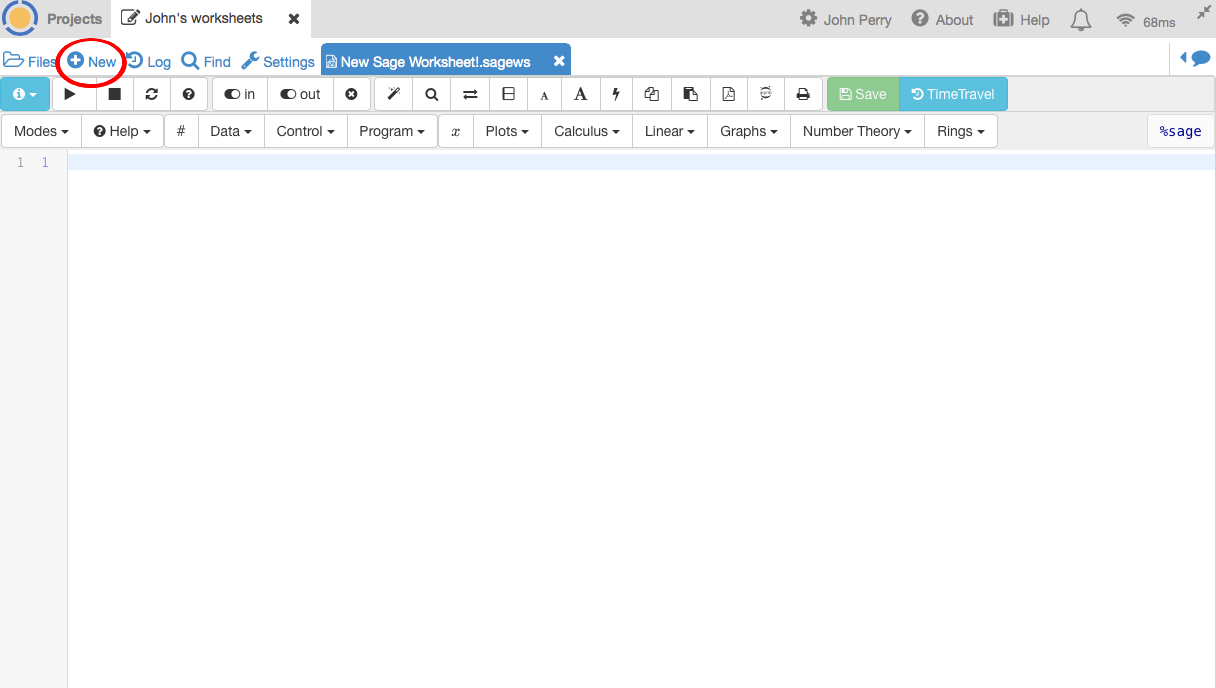
\includegraphics[viewport=0bp 500bp 825bp 688bp,clip,height=1in]{graphics/screenshots/NewFileForScriptCoCalc}
\par\end{center}

In the textbox beneath the directions to, ``Name your file, folder,
or paste in a link,'' type the name \keyboardpress{calc\_utils.sage}.
Then click on ``File'' (over to the right) and Sage will bring up
a new tab with that name.
\begin{center}
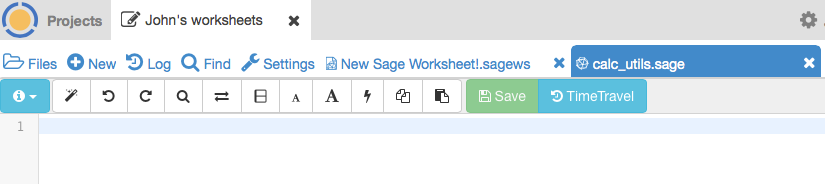
\includegraphics[height=1in]{graphics/screenshots/EmptyFileForScriptCoCalc}
\par\end{center}

Go ahead and type the procedure. If you find the text too small, click
on the ``larger'' \keyboardpress{A} beneath \keyboardpress{Settings}
in the screenshot below. That will make the text larger.\footnote{One of the authors routinely clicks this six to eight times, and that's
not because he's old. \textemdash{} Well, not \emph{that} old.}
\begin{center}
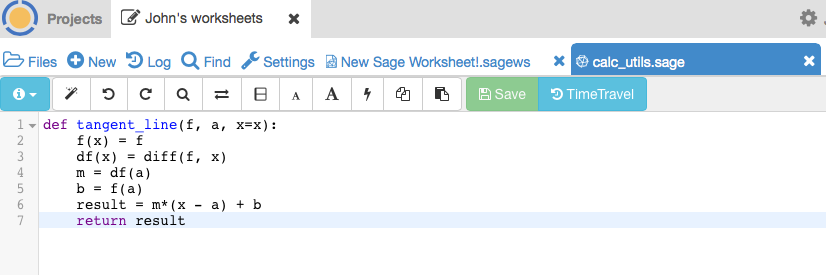
\includegraphics[height=1.5in]{graphics/screenshots/WrittenScriptCocalc}
\par\end{center}

Save it. (It should actually save automatically every few moments,
but it never hurts to give the button an extra click.)
\end{itemize}
Once you have written and saved your script, you can turn to a Sage
session (either at the command line or in the worksheet) and, at this
point, type the following (don't actually type until you read what
appears below):
\begin{sageinteraction}

\sageinput{\%attach /path/to/file/calc\_utils.sage}

\end{sageinteraction}

\noindent \emph{Before you actually do this,} we want to describe
two potential errors, as well as indicate a convention you should
be aware of.

First, the convention. We have written \keyboardpress{/path/to/file/}
as a ``template'' for you to fill in. It's basically a fill-in-the-blank
used commonly as an indication that you have to fill in the correct
value:
\begin{itemize}
\item If you're using Sage from a worksheet from an independent server,
you need to ask your instructor or the server's administrator.
\item If you're using Sage from the command line, you should try \keyboardpress{'\textasciitilde /SageScripts'},
as that corresponds to the directory we suggested earlier.\footnote{The tilde character (\keyboardpress{\textasciitilde}) is a standard
way to reference a user's home directory. We had suggested creating
a directory named \keyboardpress{SageScripts} in your home directory,
so that should do the trick.}
\item If you're using the CoCalc server \emph{and} you followed our directions
above, \emph{you need not type }\keyboardpress{/path/to/file}\emph{
at all!} Otherwise, if you created a special directory to keep your
Sage scripts, you need to type the path to that directory.
\end{itemize}
Once we move past this convention, we move to the possible errors.

If you are in the wrong directory, or you typed the filename wrong,
or you didn't follow our advice above to wait to type that in, you
will likely see an error along these lines:\index{IOError@\sageconstant{IOError}!did not find file@\sageword{did not find file \ldots{} to attach}}
\begin{sageinteraction}

\sageinput{\%attach /path/to/file/calc\_util.sage}

\sageerror{IOError: did not find file u'calc\_util.sage' to attach}

\end{sageinteraction}

\noindent This indicates that there is something wrong in what you
filled in for \keyboardpress{/path/to/file/} or in the filename itself.
In this particular example, both are wrong: we didn't actually change
\keyboardpress{/path/to/file/} to the correct path, \emph{and} we
left the \keyboardpress{s} off the filename \keyboardpress{calc\_utils.sage}~.

Now for the second error. We sometimes type things wrong. That's alright;
it's part of being human; no need to get worked up about it. After
all, the computer will get worked up on its own. It is possible to
type something wrong, and when that happens, you will get a Syntax
error. A common one for beginners will likely be this one:\index{IndentationError@\sageconstant{IndentationError}!unindent does not match any outer indentation level@\sageword{unindent does not match any outer indentation level}}
\begin{sageinteraction}

\sageinput{\%attach /path/to/file/calc\_utils.sage}

\sageerror{IndentationError: unindent does not match any outer indentation level}

\end{sageinteraction}

\noindent In this case, pay attention to the line where Sage complained,
and make sure the indentation lines up with a previous block of code.
A similar error will be this one:
\begin{sageinteraction}

\sageinput{\%attach /path/to/file/calc\_utils.sage}

\sageerror{~~~~~b = f(a)}

\sageerror{~~\textasciicircum}

\sageerror{SyntaxError: invalid syntax}

\end{sageinteraction}

\noindent This should \emph{not} happen to you, but in case it does,
and everything looks exactly perfect: the problem is that you copied
and pasted text. Appearances in a text editor can be deceiving, and
when you copy from one file to another, you can pick up hidden formatting
characters, or something similar. The solution in this case is to
eliminate the hidden formatting character by deleting those spaces,
then retyping them.

With those clarifications out of the way, now try to load the file.
If all goes well, Sage will remain silent. You should then be able
to execute your procedure in the usual way:
\begin{sageinteraction}

\sageinput{\%attach /path/to/file/calc\_utils.sage}

\sageinput{tangent\_line(x{*}{*}2, 2)}

\sageoutput{4{*}x - 4}

\end{sageinteraction}

Once you successfully attach \keyboardpress{calc\_utils.sage} to
a Sage session, you can make changes to it and Sage will automatically
incorporate the changes, leaving a message along these lines:
\begin{sageinteraction}

\sageoutput{\#\#\# reloading attached file calc\_utils.sage modified at 08:39:00
\#\#\#}
\end{sageinteraction}


\section*{Interactive worksheets}

\index{interactive worksheets|(}If you're working in a Sage worksheet,
you have access to a feature that lets you create an easily-manipulated
demonstration. We call this feature \emph{interactive worksheets}.
An interactive worksheet has one or more \emph{interactive procedures}
that allow the user to manipulate their arguments in a ``hands-on''
way through interface objects like text boxes, sliders, and so forth.
Aside from the procedure itself, there are two key steps to creating
an interactive worksheet:
\begin{itemize}
\item On the line before the procedure, but in the same cell, type \sageword{@interact}~.\index{interact@\sageword{"@interact}|see {interactive worksheets}}
\item Decide which of the following interface objects you want, and supply
the procedure with ``optional'' arguments whose default values are
initialized to these objects:
\begin{itemize}
\item an input box (to provide a value)
\item a slider (to select a value from a range)
\item a checkbox (to turn some property on or off)
\item a selector (to select some property out of several)
\item a color selector (to\ldots{} well, hopefully the reason for this is
obvious)
\end{itemize}
\end{itemize}
You will find templates for these object in Figure~\ref{fig: templates for interface objects},
and some common options for all the elements in Figure~\ref{fig: options common to interface objects}.
\begin{figure}
\begin{centering}
\begin{tabular}{|c|l|}
\hline 
\sageword{input\_box()} & %
\begin{minipage}[c][1.5\height]{0.6\columnwidth}%
a box for the user to type values, usually numbers; specific options
include
\begin{itemize}
\item \sageword{width=}\emph{box's width} (104)
\end{itemize}
%
\end{minipage}\tabularnewline
\hline 
\sageword{slider(}\emph{a}\sageword{,}\emph{b}\sageword{)} & %
\begin{minipage}[c][1.5\totalheight]{0.6\columnwidth}%
a line with a knob the user can slide left and right, ranging from
$a$ to $b$ with intermediate values%
\end{minipage}\tabularnewline
\hline 
\sageword{slider(}\emph{a\sageword{,}b}\sageword{, default=}\emph{c}\sageword{)} & %
\begin{minipage}[c][1.5\totalheight]{0.6\columnwidth}%
similar to \sageword{slider(}\emph{a}\sageword{,}\emph{b}\sageword{)},
but the user can only slide in increments of \emph{c}%
\end{minipage}\tabularnewline
\hline 
\sageword{slider(}\emph{L}\sageword{)} & %
\begin{minipage}[c][1.5\height]{0.6\columnwidth}%
similar to \sageword{slider(}\emph{a}\sageword{,}\emph{b}\sageword{)},
but the user can only select options in the collection \emph{L} (we
are still not telling you what a collection is, but you can still
use a tuple, as before)%
\end{minipage}\tabularnewline
\hline 
\sageword{range\_slider(}\emph{a}\sageword{,}\emph{b}\sageword{)} & %
\begin{minipage}[c][1.5\height]{0.6\columnwidth}%
similar to \sageword{slider(}\emph{a}\sageword{,}\emph{b}\sageword{)},
but the user selects a subinterval $\left[c,d\right]$ of $\left[a,b\right]$%
\end{minipage}\tabularnewline
\hline 
\begin{minipage}[c]{0.25\columnwidth}%
\sageword{range\_slider(}\emph{a}\sageword{,}\emph{b}\sageword{,}

\sageword{~~~default=(}$c$\sageword{,}$d$\sageword{))}%
\end{minipage} & %
\begin{minipage}[c][1.5\height]{0.6\columnwidth}%
similar to \sageword{range\_slider(}\emph{a}\sageword{,}\emph{b}\sageword{)},
but the default subinterval is $\left[c,d\right]$%
\end{minipage}\tabularnewline
\hline 
\sageword{checkbox()} & %
\begin{minipage}[c][1.5\height]{0.6\columnwidth}%
a box that the user can click on or off%
\end{minipage}\tabularnewline
\hline 
\multirow{1}{*}{\sageword{selector()}} & %
\begin{minipage}[c][1.15\height]{0.6\columnwidth}%
a drop-down menu or button bar specific options include
\begin{itemize}
\item \emph{\sageword{values=}collection of values to select from}
\item \sageword{buttons=}whether to use buttons (\sageconstant{False})
\item \sageword{nrows=}\emph{number of rows if using buttons} (1)
\item \sageword{ncols=}\emph{number of columns if using buttons} (depends
on number)
\item \sageword{width=}\emph{button's width, if buttons} (depends on value)
\end{itemize}
%
\end{minipage}\tabularnewline
\hline 
\sageword{Color(}\emph{name}\sageword{)} & %
\begin{minipage}[c][1.5\height]{0.6\columnwidth}%
a button that pops up a color chooser; default color is the one supplied
by \emph{name}, such as \sageword{'red'}%
\end{minipage}\tabularnewline
\hline 
\sageword{Color(}\emph{r}\sageword{,}\emph{g}\sageword{,}\emph{b}\sageword{)} & %
\begin{minipage}[c][1.5\height]{0.6\columnwidth}%
same as \sageword{Color(}\emph{name}\sageword{)}, but the default
color is the red-green-blue combination given by \emph{r}, \emph{g},
\emph{b}%
\end{minipage}\tabularnewline
\hline 
\end{tabular}
\par\end{centering}
\caption{\label{fig: templates for interface objects}Templates for interface
objects in an interactive procedure\index{interactive worksheets!available interface objects}}
\end{figure}
\begin{figure}
\begin{centering}
\begin{tabular}{|c|l|}
\hline 
\sageword{label=}\emph{string} & a label, placed to the left; it may include \LaTeX\ between dollar
signs\tabularnewline
\hline 
\sageword{default=}\emph{value} & the object's initial value\tabularnewline
\hline 
\end{tabular}
\par\end{centering}
\caption{\label{fig: options common to interface objects}Options common to
all interface objects in an interactive procedure \emph{except} \protect\sageword{Color()}}
\end{figure}
 \emph{This list is not comprehensive,} as we have omitted some options
that we think you are less likely to find useful. Other interface
objects may also be available that we aren't aware of (they may have
been added after we wrote this).

Sliders and selectors are similar in that they can let you choose
from a small range of values; for instance, \sageword{slider((0,~0.25,~0.5,~0.75,~1))}
and \sageword{selector((0,~0.25,~0.5,~0.75,~1))} both let you choose
from the same list. In this case, however, a slider would be the better
choice, as you can order the values from left to right, and a slider
communicates that sense better. If the values do not fit well in a
left-to-right paradigm, you'd be better off with a selector. Also,
sliders don't label the individual values, so if you think it especially
important that each value be labeled, it's best to use a selector
even if the values \emph{do} fit the left-to-right paradigm.\footnote{Of course someone will find an exception to each of these guidelines;
they are merely recommendations.}

We illustrate this on two examples. The first is quite simple, merely
to illustrate the principle: it allows the user to type a function
$f$, and plots both $f$ and its derivative on an interval $\left[a,b\right]$.
\begin{sageinteraction}

\sageinput{@interact}

\sagemoreinput{def plot\_f\_and\_df(f=input\_box(default=x{*}{*}3,label='\$f\$'),\textbackslash}

\sagemoreinput{~~~~~~~~~~~~~~~~~~a=input\_box(default=-5,label='\$a\$'),
\textbackslash}

\sagemoreinput{~~~~~~~~~~~~~~~~~~b=input\_box(default=5,label='\$b\$'),
\textbackslash}

\sagemoreinput{~~~~~~~~~~~~~~~~~~w=slider(-19,19,1,default=0,
\textbackslash}

\sagemoreinput{~~~~~~~~~~~~~~~~~~~~~~~~~~~label='squash
factor')):}

\sagemoreinput{~~~~p = plot(f, a, b, color='black')}

\sagemoreinput{~~~~df = diff(f)}

\sagemoreinput{~~~~p = p + plot(df, a, b, color='red')}

\sagemoreinput{~~~~show(p, aspect\_ratio=(20-w)/20)}

\end{sageinteraction}

\noindent If you type this into a Sage worksheet correctly, you should
see something akin to Figure~\ref{fig: squashed horizontally}.
\begin{figure}
\begin{centering}
\includegraphics[height=3in]{\string"graphics/function graphics/interactive_f_and_df\string".jpg}
\par\end{centering}
\caption{\label{fig: squashed horizontally}An unfortunate squashing}
\end{figure}
 You can see that the input boxes have nicely-formatted labels. (As
you may have guessed from our use of dollar signs, it's relying on
\LaTeX.) Unfortunately, that's not an especially clear plot; it's
a bit too squashed horizontally. We can fix this by moving the squash
factor right; if you slide the knob on the ``squash factor'' slider
all the way to the right, you get a rather nice picture the moment
you let go:
\begin{center}
\includegraphics[height=1.5in]{\string"graphics/function graphics/interactive_f_and_df_unsquashed\string".pdf}
\par\end{center}

\noindent You can also change $f$, $a$, and $b$, but they're input
boxes, so rather than sliding anything, you have to change the text.
As $a<b$ you should get a reasonable-looking graph the moment something
changes. Try another function, such as $\sin x$, with $a=0$ and
$b=2\pi$, and the graph should change to this (make sure you also
change the squash factor back to 0):
\begin{center}
\includegraphics[height=1.5in]{\string"graphics/function graphics/interactive_f_and_df_sinx\string".pdf}
\par\end{center}

You can of course call procedures you've defined from inside an interactive
procedure. Let's write an interactive procedure that plots $f$ and
its derivative on $\left[a,b\right]$, \emph{as well as} a line tangent
to $f$at a point $c$ somewhere between $a$ and $b$. We can call
the \sageword{tangent\_line()} procedure we already wrote to generate
the tangent line. While we're at it, we'll switch the defaults to
$\sin\left(x\right)$ over $\left[0,2\pi\right]$.
\begin{sageinteraction}

\sageinput{@interact}

\sagemoreinput{def plot\_f\_and\_df(f=input\_box(default=sin(x),label='\$f\$'),
\textbackslash}

\sagemoreinput{~~~~~~~~subint=range\_slider(-10,10,default=(0,2{*}pi), \textbackslash}

\sagemoreinput{~~~~~~~~~~~~label='\$(a,b)\$'), \textbackslash ~~~~~~~~t=slider(0,1,default=0.375,label='\$t\$'),
\textbackslash}

\sagemoreinput{~~~~~~~~w=slider(-19,19,1,default=0,label='squash factor')):}

\sagemoreinput{~~~~(a,b) = subint}

\sagemoreinput{~~~~p = plot(f, a, b, color='black')}

\sagemoreinput{~~~~df = diff(f)}

\sagemoreinput{~~~~p = p + plot(df, a, b, color='red')}

\sagemoreinput{~~~~\# c tells us how far to move along the interval {[}a,b{]}}

\sagemoreinput{~~~~\# 0 means a; 1 means b; values in between proportional}

\sagemoreinput{~~~~c = a + t{*}(b-a)}

\sagemoreinput{~~~~p = p + plot(tangent\_line(f, c), a, b)}

\sagemoreinput{~~~~show(p, aspect\_ratio=(20-w)/20)}

\end{sageinteraction}

\noindent When you try this in Sage, you should see the following:
\begin{center}
\includegraphics[height=3in]{\string"graphics/function graphics/interactive_f_and_df_sinx_parametric_c\string".jpg}
\par\end{center}

You may have noticed that we didn't have the user specify the point
$c$ directly. Instead, she specifies $c$ \emph{indirectly,} by choosing
a value $t$ from~0 to~1. The code then calculates a value of $c$
between $a$ and $b$ using the following parametrization:
\[
c=a+t\left(b-a\right).
\]
This parametrization is an enormously useful tool, in part because
it is relatively easy:
\begin{itemize}
\item when $t=0$, then $c=a+0=a$;
\item when $t=1$, then $c=a+\left(b-a\right)=b$;
\item when $t=.5$, then $c=a+.5\left(b-a\right)=.5a+.5b=\nicefrac{a+b}{2}$,
halfway between $a$ and $b$;
\item and so forth.
\end{itemize}
\begin{center}
\includegraphics[height=2in]{\string"graphics/function graphics/interactive_f_and_df_sinx_parametric_c=0\string".pdf}\includegraphics[height=2in]{\string"graphics/function graphics/interactive_f_and_df_sinx_parametric_c=0_5\string".pdf}\includegraphics[height=2in]{\string"graphics/function graphics/interactive_f_and_df_sinx_parametric_c=1\string".pdf}
\par\end{center}

\noindent Experiment with the slider to see how various values of
$t$ naturally let the user select a good point between $a$ and $b$.

We haven't shown how all the interface objects work, but we have shown
the ones we think are most important, as well as an elegant way to
have the user select a point in an interval without having to check
whether the point actually lies in the interval. We encourage you
to experiment with the other objects, especially selecting a color.\index{interactive worksheets|)}

\section*{Exercises}

\subsection*{True/False. If the statement is false, replace it with a true statement.}
\begin{lyxlist}{99.}
\item [{1.}] Procedures allow us to reuse common groups of commands.
\item [{2.}] If an argument holds the value of some variable outside the
procedure, changing the argument's value also changes that variable's
value.
\item [{3.}] Sage allows you to specify optional arguments.
\item [{4.}] If a Sage procedure does not explicitly \sageword{return}
a value, then it returns \sageconstant{None}.
\item [{5.}] When we pass indeterminates as arguments to Sage procedures,
we must redefine any mathematical functions that depend on them.
\item [{6.}] User-defined procedures cannot use Sage procedures.
\item [{7.}] No one uses pseudocode in real life.
\item [{8.}] Pseudocode communicates ideas using ``plain English'' and
mathematical symbols, rather than a particular language's symbols
and formats.
\item [{9.}] The best way to reuse a group of Sage procedures in different
sessions is to copy-and-paste the code.
\item [{10.}] The \sageword{\%attach} command allows Sage to read and
execute a script, as well as automatically reload it when you change
it.
\item [{11.}] You can use interactive procedures from command-line Sage.
\item [{12.}] If the user has to select from 100 equally-spaced values
on a number line, it's best to use a slider.
\item [{13.}] If the user has to select a function from the set $\left\{ \sin x,\cos x,\ln x,e^{x}\right\} $,
it's best to use a selector.
\item [{14.}] To find the number one-fourth of the distance from $2$ to
$10$, substitute $t=0.25$ into the expression $2+8t$.
\item [{15.}] A disadvantage to interactive procedures is that you can't
break up their tasks into tasks performed by other procedures.
\end{lyxlist}

\subsection*{Multiple Choice}
\begin{lyxlist}{99.}
\item [{1.}] We start the definition of a procedure in Sage using:
\begin{lyxlist}{M.}
\item [{A.}] \textbf{algorithm}
\item [{B.}] its type
\item [{C.}] its name
\item [{D.}] \sageword{def}
\end{lyxlist}
\item [{2.}] The format for an optional argument is:
\begin{lyxlist}{M.}
\item [{A.}] not to list it
\item [{B.}] to preface its identifier with the keyword \sageword{optional}
\item [{C.}] to preface the procedure name with the keyword \sageword{def}
\item [{D.}] to place \sageword{=} after its identifier, followed by a
default value
\end{lyxlist}
\item [{3.}] Which of the following is not an accurate description of an
argument?
\begin{lyxlist}{M.}
\item [{A.}] a stand-in for a variable outside the procedure, whose value
the procedure can change
\item [{B.}] a copy of some data outside the procedure
\item [{C.}] a variable whose value you may not know in advance
\item [{D.}] information the procedure may or may not need to perform its
tasks
\end{lyxlist}
\item [{4.}] The best way to report a procedure's result back to the client
is to
\begin{lyxlist}{M.}
\item [{A.}] list the result in a \sageword{return} statement
\item [{B.}] assign the value to one of the arguments
\item [{C.}] assign it to a global variable called \sageword{result}
\item [{D.}] assign a value to the procedure's name
\end{lyxlist}
\item [{5.}] A procedure that lacks a \sageword{return} statement:
\begin{lyxlist}{M.}
\item [{A.}] raises an error
\item [{B.}] returns the empty set
\item [{C.}] returns \sageconstant{None}
\item [{D.}] does nothing special
\end{lyxlist}
\item [{6.}] When a list of commands is subject to a keyword that starts
a control structure, such as \sageword{def}, you should:
\begin{lyxlist}{M.}
\item [{A.}] indent the commands in question
\item [{B.}] add a colon at the end of the control structure's statement
\item [{C.}] reverse the indentation when the list is finished
\item [{D.}] all of the above
\end{lyxlist}
\item [{7.}] Which of the following properties does our pseudocode standard
share with Sage code?
\begin{lyxlist}{M.}
\item [{A.}] Statements subject to control structures are indented.
\item [{B.}] We can use \sageword{def} in both pseudocode and Sage code.
\item [{C.}] We specify the inputs' types in Sage, just as we specify which
set an input comes from in pseudocode.
\item [{D.}] all of the above
\end{lyxlist}
\item [{8.}] The best way in Sage to substitute for an indeterminate that
was passed as an argument is by:
\begin{lyxlist}{M.}
\item [{A.}] function-call substitution
\item [{B.}] dictionary substitution
\item [{C.}] keyword assignment
\item [{D.}] function-call substitution \emph{after} redefining the function
\end{lyxlist}
\item [{9.}] Which of the following identifiers can we \emph{not} assign
values to?
\begin{lyxlist}{M.}
\item [{A.}] a valid identifier
\item [{B.}] a keyword
\item [{C.}] a constant
\item [{D.}] the name of a procedure that is already defined
\end{lyxlist}
\item [{10.}] When the user changes a setting in an interactive procedure,
the only guaranteed effect is to change what part of the procedure?
\begin{lyxlist}{M.}
\item [{A.}] a global variable
\item [{B.}] a local variable
\item [{C.}] an argument of the procedure
\item [{D.}] the procedure's name
\end{lyxlist}
\end{lyxlist}

\subsection*{Short answer}
\begin{lyxlist}{9.}
\item [{1.}] Explain modularity and why it is a good practice when writing
programs.
\item [{2.}] Are modularity and modular arithmetic the same thing?
\end{lyxlist}

\subsection*{Programming}
\begin{lyxlist}{9.}
\item [{1.}] Sage does not automatically add arrowheads to a curve. Since
the derivative tells us the slope of the curve at a given point, we
can determine what directions arrows at the end should point by computing
derivatives at the endpoints and putting arrows there. Write a procedure
\sageword{arrowplot()} that takes as argument a function $f$, two
endpoints $a$ and $b$, and an ``arrow length'' $\Delta x$, then
plots $f$ on $\left[a,b\right]$, adding arrowheads using the principle
that $\left(a,f\left(a\right)\right)$ and $\left(a-\Delta x,f\left(a\right)-f'\left(a\right)\Delta x\right)$
would give us two points on a line tangent to $f$ at $a$ (and which
would specify a suitable arrow). (We leave it to you to modify this
definition for an arrowhead at $b$.)
\item [{2.}] \label{exc: normal line function}Write pseudocode for a procedure
that computes and returns the normal line to $f$ at $x=c$. Then:
\begin{lyxlist}{(m)}
\item [{(a)}] Implement this in Sage code.
\item [{(b)}] Pick any transcendental function $f$, and any point $c$
where $f$ is transcendental.
\item [{(c)}] Use this code and the \sageword{tangent\_line()} procedure
to plot both the normal and tangent lines to $f$ at $x=c$.
\item [{(d)}] Write an interactive procedure to sketch the graph of a function,
a tangent line at a point $x=c$, and the normal line at $x=c$. Aside
from any obvious interface elements needed, include at least a slider
to control the aspect ratio of the resulting graph.
\end{lyxlist}
Your implementation will sometimes fail; for instance, if you use
$f=\left(x-1\right)^{2}+2$ and $c=1$, you should encounter a \sageconstant{ZeroDivisionError}.
\begin{center}
\textcolor{red}{\huge{}DON'T PANIC!}{\huge\par}
\par\end{center}

You should actually \emph{expect} this error, since computing a perpendicular
requires a reciprocal, which means division, which opens the possibility
of division by zero. We address this issue in Chapter~\ref{chap: decision making}
on Decision-Making. Make sure your code works with functions and points
that don't misbehave.
\item [{3.}] Write pseudocode for a procedure named \emph{avg\_value} whose
inputs are a function $f$, and indeterminate $x$, and the endpoints
$a$ and $b$ of an interval $I$. The procedure returns the average
value of $f$ on the interval. (You may need to review some calculus
to solve this problem.)
\item [{4.}] Let's define the operation $a*b=ab+\left(a+2b+1\right)$.
\begin{lyxlist}{(m)}
\item [{(a)}] Write pseudocode for a procedure named \sageword{star()}that
accepts two integers $a$ and $b$ and returns $a*b$.
\item [{(b)}] Implement this pseudocode as a Sage procedure.
\item [{(c)}] Test your procedure on several different values of $a$ and
$b$.
\item [{(d)}] Is there a value of $a$ such that $a*b=b$, regardless of
the value of $b$?
\end{lyxlist}
\item [{5.}] Write a Sage procedure named \sageword{dotted\_line\_segment()}
that accepts seven arguments named \sageword{x1}, \sageword{y1},
\sageword{x2}, \sageword{y2}, \sageword{color}, \sageword{pointsize},
and \sageword{pointcolor}. The colors' default values should be \sageword{'black'},
and the default color of \sageword{pointsize} should be 60. The procedure
returns the sum of:
\begin{itemize}
\item a line segment that connects those points and whose color is \sageword{color},
and
\item two points, both of color \sageword{pointcolor} and of size \sageword{pointsize},
whose locations are $\left(x_{1},y_{1}\right)$ and $\left(x_{2},y_{2}\right)$.
\end{itemize}
\begin{lyxlist}{(m)}
\item [{(a)}] Use this procedure to plot a line segment connecting the
points $\left(0,0\right)$ and $\left(1,4\right)$ whose color and
point color are both black.
\item [{(b)}] Use this procedure to plot a black line segment connecting
the red points $\left(0,6\right)$ and $\left(2,0\right)$.
\end{lyxlist}
You need not write pseudocode for this procedure.
\item [{6.}] \label{exc: taylor truncated 4}Implement the following pseudocode
in Sage.
\begin{pseudocode}

\textbf{algorithm} \emph{Taylor\_Truncated4}

\textbf{inputs}
\begin{itemize}
\item $a\in\mathbb{R}$
\item $x$, an indeterminate
\item $f$, a function in $x$ that is integrable at $x=a$
\end{itemize}
\textbf{outputs}
\begin{itemize}
\item the truncated Taylor series for $f\left(x\right)$ around $x=a$
\end{itemize}
\textbf{do}

\quad let \emph{result} = $f\left(a\right)$

\quad add $f'\left(a\right)\cdot\left(x-a\right)$ to \emph{result}\footnote{Here's a hint on this one. To ``add \ldots{} to result'' use the
construction \sageword{result = result +}\ldots}

\quad add $f''\left(a\right)\cdot\left(x-a\right)^{2}/2$ to \emph{result}

\quad add $f'''\left(a\right)\cdot\left(x-a\right)^{3}/6$ to \emph{result}

\quad add $f^{\left(4\right)}\left(a\right)\cdot\left(x-a\right)^{4}/24$
to \emph{result}

\quad \textbf{return} \emph{result}
\end{pseudocode}

Check it by finding the truncated Taylor series for $e^{x}$ at $x=1$,
and comparing the truncated series' value at $x=1.1$ with the value
of $e^{1.1}$.
\item [{7.}] Explain how the ``squash factor'' we used in our interactive
procedures was used to set the aspect ratio of the plot. Your explanation
should address why the leftmost value squashes the graph as far left
as possible, why the rightmost value stretches the graph as far right
as possible, and why the middle value sits somewhere in between.
\end{lyxlist}

\chapter{Repeating yourself definitely with collections}

\label{chap: definite loops}There are a number of cases where you
want to repeat a task several times. A classic example comes from
differential equations; suppose we know
\[
\nicefrac{dy}{dx}=\sin y+2\cos x,
\]
that is, at any point $\left(x,y\right)$, the value of $y$ is changing
by $\sin y+2\cos x$. It is difficult, and often impossible, to find
the exact formula for $y$ in terms of $y$, so it is necessary to
approximate ``future'' values of $y$ from a starting point $\left(x,y\right)$.\footnote{For instance, this is how weather prediction works.}
In this case you usually decide to make a number of very small ``steps
forward'' with $x$, and re-evaluate $y$ at each point, tracing
out the resulting behavior. In this case, suppose we start at $\left(0,0\right)$;
then $y'\left(0,0\right)=2$, which suggests the function wants to
move forward along a line with slope~2. After all, you're computing
the derivative, which is the slope of the tangent line, which goes
in the same direction as the curve at that point. This technique of
moving along the tangent line is known as \textbf{\index{Euler's Method}Euler's
Method}.

However, the curve wants to go in the same direction as its tangent
line only for a moment; as soon as we step off the point $\left(0,0\right)$,
the derivative changes ever-so-slightly, and the tangent line is no
longer valid. To avoid making too much error, we take a tiny step,
say $\Delta x=\nicefrac{1}{10}$, along this line, which takes us
to the point $\left(.1,.2\right)$. Here, $y'\left(.1,.2\right)\approx2.1$,
so we step out along a line of slope~2.1, which takes us to the point
$\left(.2,.41\right)$. Here, $y'\left(.2,.41\right)\approx2.0$,
which takes us to $\left(.3,.61\right)$. Here, $y'\left(.3,.61\right)\approx1.9$,
which takes us to $\left(.4,.8\right)$. Here, $y'\left(.4,.8\right)\approx1.8$,
which takes us to $\left(.5,.98\right)$. Here, $y'\left(.5,.98\right)\approx1.6$,
which takes us to $\left(.6,1.14\right)$. Go far enough, and you'll
trace out a picture something like this:
\begin{center}
\includegraphics[height=1.5in]{graphics/definite_loops_graphics/approximation_to_siny+2cosx}
\par\end{center}

\noindent To generate this curve, we used a step size of $\Delta x=\nicefrac{1}{10}$.
Repeat the process from $\left(0,0\right)$ with a smaller step size,
say $\Delta x=\nicefrac{1}{100}$, and you'll get a slightly different
result:
\begin{center}
\includegraphics[height=1.5in]{graphics/definite_loops_graphics/approximation_to_siny+2cosx_comparison}
\par\end{center}

\noindent This reflects the fact that our approximation incorporates
some error. Still, it's not \emph{that} bad; the approximations are
pretty close. Then again, we obtained the blue curve using~80 points,
and the red curve using~800 points. You don't want to do that by
hand, do you?

When a task (or set of tasks) has to be repeated more than once on
the result of the previous application, we call this repetition \textbf{iteration}\index{iteration}.
Iteration pops up repeatedly in computational mathematics, so programming
languages typically offer a control structure called a \textbf{\index{loop}loop}.
Unlike Euler's method, we don't always know in advance how many times
the loop must repeat, so many loops are \textbf{\index{indefinite loop}}\index{loop!indefinite}\textbf{indefinite}.
Nevertheless, it is very often the case that we can determine the
exact number of times a task must repeat from the outset; we call
this a \textbf{\index{definite loop}}\index{loop!definite}\textbf{definite
loop}. This chapter introduces definite loops; we postpone indefinite
loops for Chapter \ref{chap: indefinite loops}.

\section*{How to make a computer repeat a fixed number of times?}

\subsection*{Pseudocode}

We can describe Euler's Method in pseudocode as follows.
\begin{pseudocode}

\textbf{algorithm} \emph{Eulers\_method}

\textbf{inputs}
\begin{itemize}
\item $d\!f$, the derivative of a function
\item $\left(x_{0},y_{0}\right)$, initial values of $x$ and $y$
\item $\Delta x$, step size
\item $n$, number of steps to take
\end{itemize}
\textbf{outputs}
\begin{itemize}
\item approximation to $\left(x_{0}+n\Delta x,f\left(x_{0}+n\Delta x\right)\right)$
\end{itemize}
\textbf{do}

\quad let $a=x_{0}$, $b=y_{0}$

\quad \textbf{repeat} $n$ times

\quad \quad add $\Delta x\cdot d\!f\left(a,b\right)$ to $b$

\quad \quad add $\Delta x$ to $a$

\quad \textbf{return} $\left(a,b\right)$
\end{pseudocode}

\noindent We use \textbf{\index{loop!pseudocode}\index{repeat}repeat}
in pseudocode to indicate that a set of tasks are to be repeated a
certain number of times, and indent the tasks to repeat.

\subsection*{Sage code}

As with most computer languages, Sage has no keyword named\texttt{
}\sageword{repeat}.\footnote{Our use of \textbf{repeat} is meant to illustrate how pseudocode aims
for clarity of communication, rather than mimicry of a particular
language, and it is not unheard-of to see \textbf{repeat} used in
pseudocode. That said, some programming languages do feature a \keyboardpress{repeat}
structure for loops.} For definite loops, Sage uses a more general-purpose keyword, \sageword{for}.
When you know you are to repeat a task $n$ times, the construction
is fairly simple:\index{keyword!for@\sageword{for}}
\begin{center}
\sageword{for}\emph{variable}\sageword{~in range(n):}
\par\end{center}

\noindent For \emph{variable} you choose an identifier that will hold
the number of the loop each time you pass through it.

We can now implement Euler's Method in Sage:
\begin{sageinteraction}

\sageinput{def eulers\_method(df, x0, y0, Delta\_x, n):}

\sagemoreinput{~~~~\# starting point}

\sagemoreinput{~~~~a, b = x0, y0}

\sagemoreinput{~~~~\# compute tangent lines \& step forward}

\sagemoreinput{~~~~for i in range(n):}

\sagemoreinput{~~~~~~~~b = Delta\_x {*} df(a, b) + b}

\sagemoreinput{~~~~~~~~a = Delta\_x + a}

\sagemoreinput{~~~~return a, b}

\end{sageinteraction}

This looks pretty straightforward. Let's try it out:
\begin{sageinteraction}

\sageinput{df(x,y) = sin(y) + 2{*}cos(x)}

\sageinput{eulers\_method(df, 0, 0, 1/10, 80)}

\end{sageinteraction}

\noindent If you do try this, you'll notice it takes an \emph{awfully
long time} to sort itself out, certainly more than a few seconds.
To see why this happens, interrupt the calculation (press the ``Stop''
button in the cloud, click the ``Action'' menu and click ``Interrupt''
on an independent server, or hold \keyboardpress{Ctrl}and press \keyboardpress{C}
at the command line) and run the code again with a smaller value of
$n$:
\begin{sageinteraction}

\sageinput{eulers\_method(df, 0, 0, 1/10, 10)}

\sageoutput{(1, 1/5{*}cos(9/10) + 1/5{*}cos(4/5) + 1/5{*}cos(7/10) + 1/5{*}cos(3/5)
+ 1/5{*}cos(1/2) \ldots}

\end{sageinteraction}

\noindent (The ellipses at the end indicate there's a lot more after
that. \emph{Quite} a lot more!)

Do you see what's going on? Sage is computing exact values; and the
exact value of this number grows more and more complicated with each
iteration. You can modify the code to simplify \sageword{b} after
each computation, but it doesn't really help. This simply illustrates
a drawback of symbolic computation: to gain ``exact'' values, you
sacrifice time. But there's no need to sacrifice that here! After
all, we're approximating the value anyway. In that case, let's turn
to floating-point values, and see if that speeds things up. Let's
replace \sageword{1/10} by \sageword{.1}, and let's see how it turns
out.
\begin{sageinteraction}

\sageinput{eulers\_method(df, 0, 0, .1, 80)}

\sageoutput{(7.99999999999999, 4.340418570291038)\label{sage: result from eulers method}}

\end{sageinteraction}

This comes to $\left(8,4.34\right)$. Not only did we obtain an answer
quickly, it was nearly instantaneous! It's clearly a better idea to
rely on floating-point when you know you're approximating anyway.

\subsection*{What just happened?}

What takes place when we execute a loop? Let's examine what happens,
looking closely at the values of $a$ and $b$ each time we pass through
the loop.

When we ran the program, both $a$ and $b$ take on the value~0,
because that's what we passed as the arguments for the initial value.
We next come to the line
\begin{center}
\sageword{for i in range(n):}
\par\end{center}

\noindent Recall that this instructs Sage to repeat the subsequent
tasks $n$ times. The value of the loop is stored in the variable
$i$, in case you need it; we don't need $i$ for this problem, but
a later example will illustrate how this can be useful.

Now, $n$ is an argument, and in this case we assigned it the value~80.
So the indented tasks will repeat~80 times. We now illustrate what
occurs the first few times:
\begin{lyxlist}{When i=9:}
\item [{When~$i=0$:}] The first line tells Sage to compute $\Delta xd\!f\left(a,b\right)$
and add it to $b$, then assign the result to $b$. After this, $b=.1f\left(0,0\right)+0=.2$.\\
The second line tells Sage to add $\Delta x$ to $a$, then assign
the result to $a$. After this, $a=.1+0=.1$.
\item [{When~$i=1$:}] The first line tells Sage to compute $\Delta xd\!f\left(a,b\right)$
and add it to $b$, then assign the result to $b$. After this, $b=.1f\left(.1,.2\right)+.2\approx.42$.\\
The second line tells Sage to add $\Delta x$ to $a$, then assign
the result to $a$. After this, $a=.1+.1=.2$.
\item [{When~$i=2$:}] The first line tells Sage to compute $\Delta xd\!f\left(a,b\right)$
and add it to $b$, then assign the result to $b$. After this, $b=.1f\left(.2,.42\right)+.42\approx.66$.\\
The second line tells Sage to add $\Delta x$ to $a$, then assign
the result to $a$. After this, $a=.1+.2=.3$.
\end{lyxlist}
\ldots and so forth. Repeat this 80 times, and you end up with the
value that Sage reported.

\section*{How does this work? \emph{or,} an introduction to collections}

We discuss in more detail how this process works. Definite loops work
by passing over a collection; in general, you can use the \sageword{for}
keyword in the form\index{keyword!for@\sageword{for}}
\begin{center}
\emph{\sageword{for}variable \sageword{in}collection}\sageword{:}
\par\end{center}

\noindent and Sage will perform the following, indented tasks as many
times as there are objects in \emph{collection}. On the first pass
through the loop, \emph{variable} takes on the value of the ``first''
element of \emph{collection}; on each subsequent pass, \emph{variable}
takes on the value of the element in \emph{collection} that ``follows''
the current value of \emph{variable}.

We put ``first'' and ``follows'' in quotes because in some collections,
what Sage considers the ``first'' element may not be what you expect,
and the value it considers to ``follow'' the current value may not
be what you consider to follow it. This is not such a problem as you
may think, since it happens only in collections where you should not
be expecting a ``first,'' ``second,'' etc. We'll talk about that
in a second.

\subsection*{But what is a collection?}

As you'd expect from its name, a \textbf{collection\index{collection}}
is an object that ``contains'' other objects. We can classify collections
in two ways.
\begin{itemize}
\item The first classification is whether a collection is indexed\index{collection!indexing}.
\begin{itemize}
\item \textbf{Indexed} collections order their elements that allow you to
access any element according to its location.
\item \textbf{Unindexed} collections do not order their elements, so you
can access\emph{ any} element, but not by its location.
\end{itemize}
\item The second classification is whether a collection is \index{collection!mutable}mutable.
\begin{itemize}
\item \textbf{Mutable} collections allow you to change their values.
\item \textbf{Immutable} collections do not allow you to change their values.
\end{itemize}
\end{itemize}
We use five kinds of collections.

A \textbf{tuple\index{tuple}} is an indexed, immutable collection;
we refer to a tuple of $n$ elements as an $n$-tuple. You create
a tuple using parentheses or the \index{tuple()@\sageword{tuple()}}\sageword{tuple()}
command, inserting another collection between its parentheses; for
instance, the following two commands do the same thing:
\begin{sageinteraction}

\sageinput{a\_tuple = (3, pi, -I)}

\sageinput{b\_tuple = tuple({[}3, pi, -I{]})}

\sageinput{a\_tuple == b\_tuple}

\sageoutput{True}

\end{sageinteraction}

\noindent You can also create an ``empty tuple'' by placing nothing
between the parentheses, either \sageword{()} or \sageword{tuple()}.
As immutable collections, tuples are useful for communicating data
that should not be changed; i.e., constants. You have already seen
and used tuples; we used them extensively to provide points to the
plotting commands.

A \textbf{list\index{list}} is an indexed, mutable collection. You
create a list using brackets or the \sageword{list()}\index{list()@\sageword{list()}}
command, inserting another collection between the brackets or parentheses;
for instance,
\begin{sageinteraction}

\sageinput{a\_list = {[}3, pi, -I{]}}

\end{sageinteraction}

\noindent You can also create an ``empty list'' by placing nothing
between the parentheses or brackets, either \sageword{{[}{]}} or
\sageword{list()}. As mutable collections, it is easy to modify both
a list and its elements. If you need to store values that might change,
you need a list, not a tuple, as you cannot modify a tuple.

A \textbf{set\index{set}} is an unindexed, mutable collection. You
create a set using braces or the \sageword{set()}\index{set()@\sageword{set()}}
command; for instance,
\begin{sageinteraction}

\sageinput{a\_set = \{3, pi, -I\}}

\sageinput{a\_set}

\sageoutput{\{-I, 3, pi\}}

\end{sageinteraction}

\noindent Notice how the elements' ``order'' changed. You can also
create an ``empty set'' by placing nothing between the parentheses,
like so: \sageword{set()}. As they are mutable, you can modify a
set. An important property of a set is that it stores only one copy
of any element; trying to add additional copies leaves us with only
one nevertheless. For example:
\begin{sageinteraction}

\sageinput{another\_set = \{2, 2, 2, 2, 2, 2\}}

\sageinput{another\_set}

\sageoutput{\{2\}}

\end{sageinteraction}

\noindent We do not use sets often in this text; while they have important
uses, they can be tricky to use, as they accept only immutable objects,\index{set!elements must be immutable}
and many Sage objects are mutable. For instance, you can store tuples
in a set, but not lists. For that matter, sets themselves are mutable,
so you cannot store one set inside another.\index{TypeError@\sageconstant{TypeError}!unhashable type@\sageword{unhashable type: \ldots}}
\begin{sageinteraction}

\sageinput{\{ a\_tuple \}}

\sageoutput{\{(3, pi, -I)\}}

\sageinput{\{ a\_set \}}

\sageerror{TypeError: unhashable type: 'set'}

\end{sageinteraction}

A \textbf{\index{set!frozen}frozen set} \index{frozen set|see{set}}is
an unindexed, immutable collection. You create a frozen set using
the \index{frozenset()@\sageword{frozenset()}}\sageword{frozenset()}
command; for instance,
\begin{sageinteraction}

\sageinput{f\_set = frozenset(a\_set)}

\sageinput{f\_set}

\sageoutput{frozenset(\{-I, 3, pi\})}

\end{sageinteraction}

\noindent You can also create an ``empty frozen set'' by placing
nothing between the parentheses, \sageword{frozenset()}. Frozen sets
are especially useful when you need sets of sets: you cannot store
a mutable set inside a set, so you store a frozen set inside a set.

A \textbf{dictionary\index{dictionary}} is like a list, in that it
is an indexed, mutable collection. It is \emph{unlike }a list in that
the indexing is by entry rather than by position. You create a dictionary
using braces \emph{and} colons; the braces delimit the dictionary,
while the colons indicate a correspondence between \textbf{keys} (dictionary
entries) and \textbf{values} (definitions for the entries). For example:
\begin{sageinteraction}

\sageinput{a\_dict = \{x:2, x\textasciicircum 2 + 1:'hello'\}}

\end{sageinteraction}

\noindent In this (rather silly) dictionary, the entry \sageword{x}
corresponds to the value \sageword{2}, while the entry \sageword{x\textasciicircum 2~+~1}
corresponds to the value \sageword{'hello'}. Another way to create
a dictionary is by using the \index{dict()@\sageword{dict()}}\sageword{dict()}
command with a collection of 2-tuples; the first entry in the tuple
becomes the key, the second becomes the value.
\begin{sageinteraction}

\sageinput{tup\_dict = dict(( (x,1), (15,-71), (cos(x),3) ))}

\sageinput{tup\_dict{[}cos(x){]}}

\sageoutput{3}

\end{sageinteraction}

\noindent You can also create an ``empty dictionary'' by placing
nothing between the parentheses of a \sageword{dict()} command, \sageword{dict()}.
We have already used dictionaries when performing \index{substitution!dictionary}dictionary
substitution.

\subsection*{How does indexing work?}

\index{indexing}\index{collection!indexing}The answer to this questions
depends somewhat on the type of collection, but it always involves
the brackets, \sageword{{[}{]}}.

For a dictionary, you type the key between the brackets, and Sage
returns the value assigned to that key:
\begin{sageinteraction}

\sageinput{a\_dict{[}x\textasciicircum 2 + 1{]}}

\sageoutput{'hello'}

\end{sageinteraction}

\noindent We can now explain how dictionary substitution works in
an expression: when you type
\begin{sageinteraction}

\sageinput{f = x\textasciicircum 2 + 2}

\sageinput{f(\{x:1\})}

\end{sageinteraction}

\noindent then Sage uses the dictionary \sageword{\{x:1\}} to interpret
every \sageword{x} in \sageword{f} as a \sageword{1} instead.

For tuples\index{tuple} and \index{list}lists, indexing has a meaning
analogous to that of a subscript in mathematics. Just as $a_{1}$,
$a_{2}$, \ldots , $a_{i}$, \ldots{} indicate the first, second, \ldots ,
$i$th, \ldots{} elements of a sequence, \sageword{LorT{[}}\emph{i}\sageword{{]}}
indicates the element in position $i$. The slight difference in wording
is important; for Sage you need to supply a ``legal position,''
which is not quite the same as you might expect:
\begin{sageinteraction}

\sageinput{a\_tuple}

\sageoutput{(3, pi, -I)}

\sageinput{a\_tuple{[}1{]}}

\sageoutput{pi}

\sageinput{a\_tuple{[}2{]}}

\sageoutput{-I}

\end{sageinteraction}

\noindent \index{indexing!numbering}If you look closely at the numbering,
you'll notice that Sage starts numbering its elements at position~0,
\emph{not} position~1. To read the first element of \sageword{a\_tuple},
you would actually type \sageword{a\_tuple{[}0{]}}.

Suppose the collection \sageword{C} is either a tuple or a list,
and has $n$ elements. The meaning of ``legal position'' corresponds
to the following table:
\begin{center}
\index{PANIC@\textcolor{red}{PANIC"!}}%
\begin{tabular}{ccccccccc}
 &  & \sageword{C{[}0{]}} & \sageword{C{[}1{]}} & \sageword{C{[}2{]}} &  & \sageword{C{[}n-2{]}} & \sageword{C{[}n-1{]}} & \sageword{C{[}n{]}}\tabularnewline
\cline{3-5} \cline{4-5} \cline{5-5} \cline{7-8} \cline{8-8} 
which element? & \multicolumn{1}{c|}{\textcolor{red}{PANIC!}} & \multicolumn{1}{c|}{first} & \multicolumn{1}{c|}{second} & \multicolumn{1}{c|}{third} & \multicolumn{1}{c|}{\ldots} & \multicolumn{1}{c|}{penultimate} & \multicolumn{1}{c|}{last} & \textcolor{red}{PANIC!}\tabularnewline
\cline{3-5} \cline{4-5} \cline{5-5} \cline{7-8} \cline{8-8} 
 & \sageword{C{[}-n-1{]}} & \sageword{C{[}-n{]}} & \sageword{C{[}-n+1{]}} & \sageword{C{[}-n+2{]}} &  & \sageword{C{[}-2{]}} & \sageword{C{[}-1{]}} & \tabularnewline
\end{tabular}
\par\end{center}

\noindent As usual, \textcolor{red}{PANIC!} stands in for, ``some
sort of error occurs!'' We discuss these in the next section, but
notice something surprising: negative indices have meaning! They take
you backwards through the elements of C. We will not make use of this
feature in this text, but there are occasions where it can be put
to good use.

\subsection*{Things you can do with collections}

We don't address here the applications of collections, so much as
the commands use can use on them, and the methods you can send them.
We've already seen how you can access elements of indexed collections
via the bracket operator.

\subsubsection*{All five collections}

Two commands and one operation are common to all five collections:
\begin{center}
\begin{tabular*}{0.8\columnwidth}{@{\extracolsep{\fill}}|>{\raggedright}m{0.25\columnwidth}|>{\raggedright}m{0.5\columnwidth}|}
\hline 
\index{len()@\sageword{len()}}\sageword{len(}\emph{collection}\sageword{)} & \index{dictionary!commands shared with all collections}\index{set!commands shared with all collections}\index{tuple!commands shared with all collections}\index{list!commands shared with all collections}the
number of elements in \emph{collection}\tabularnewline
\hline 
\emph{element} \sageword{in}\index{in@\sageword{in}}\index{collection!membership in|see{\sageword{in}}}
\emph{collection} & %
\begin{minipage}[t][10ex]{0.5\columnwidth}%
\sageword{True} if and only if \emph{element} is in collection (if
\emph{collection} is a dictionary, this means that \emph{element}
appears as a key)%
\end{minipage}\tabularnewline
\hline 
\index{max()@\sageword{max()}}\sageword{max(}\emph{collection}\sageword{)} & the largest element in \emph{collection}\tabularnewline
\hline 
\index{min()@\sageword{min()}}\sageword{min(}\emph{collection}\sageword{)} & the smallest element in \emph{collection}\tabularnewline
\hline 
\index{sorted@\sageword{sorted}}\sageword{sorted(}\emph{collection}\texttt{,
}\sageword{reverse=}\sageconstant{True} or \sageconstant{False}\sageword{)} & returns a \index{sorting}sorted copy of \emph{collection} (reverse
order if \sageword{reverse=}\sageconstant{True})\tabularnewline
\hline 
\sageword{sorted(}\emph{collection\sageword{,}key}\sageword{,}\sageword{reverse=}\sageconstant{True}
or \sageconstant{False}\sageword{)} & returns copy of \emph{collection}, sorted according to \emph{key}
(reverse order if \sageword{reverse=}\sageconstant{True})\tabularnewline
\hline 
\end{tabular*}
\par\end{center}

\noindent Most of the time, a program doesn't know beforehand how
many elements it has to work with, so having a way to determine that
number is enormously useful.
\begin{sageinteraction}

\sageinput{len(a\_set)}

\sageoutput{3}

\sageinput{len(another\_set)}

\sageoutput{1}

\sageinput{sqrt(2) in a\_list}

\sageoutput{False}

\sageinput{-sqrt(-1) in a\_tuple}

\sageoutput{True}

\sageinput{sorted(a\_tuple)}

\sageoutput{{[}3, pi, -I{]}}

\end{sageinteraction}

\noindent Notice how the \sageword{sorted()} command always returns
a list, even though we supplied a tuple for its input.

There are times when you may want to sort a collection in a manner
different from Sage's default. You can modify the sorting criteria
using the \sageword{key} option, to which you assign a procedure
that returns an object that serves as a key for sorting, much as a
dictionary. We won't use this often, but the example above illustrates
the point: from the point of view of complex analysis, it seems odd
to sort $-i$ after 3 and $\pi$, when its ``norm'' is smaller.
To sort by the norm, we can write a procedure that computes the norm
of any complex number, and use that as the key:
\begin{sageinteraction}

\sageinput{def by\_norm(z):}

\sagemoreinput{~~~~return real\_part(z){*}{*}2 + imag\_part(z){*}{*}2\label{sage fn: by_norm(z)}}

\sageinput{sorted(a\_tuple, key=by\_norm)}

\sageoutput{{[}-I, 3, pi{]}}
\end{sageinteraction}


\subsubsection*{Lists and tuples}

\index{list}\index{tuple}The next methods and operations apply only
to lists and tuples:
\begin{center}
\index{tuple!methods}\index{list!methods}%
\begin{tabular*}{0.8\columnwidth}{@{\extracolsep{\fill}}|>{\raggedright}p{0.25\columnwidth}|l|}
\hline 
\index{count@\sageword{.count()}}\emph{LorT}\sageword{.count(}\emph{element}\sageword{)} & the\index{list!commands shared with tuple}\index{tuple!commands shared with list}
number of time \emph{element} appears in \emph{LorT}\tabularnewline
\hline 
\index{index@\sageword{.index()}}\emph{LorT}\sageword{.index(}\emph{element}\sageword{)} & the location of \emph{element} in \emph{LorT}\tabularnewline
\hline 
\emph{LorT1}\sageword{+}\emph{LorT2} & \emph{}%
\begin{minipage}[c][7ex]{0.5\columnwidth}%
creates a new list/tuple whose elements are those of \emph{LorT1},
followed by those of \emph{LorT2}%
\end{minipage}\tabularnewline
\hline 
\end{tabular*}
\par\end{center}

\noindent It should make sense that you cannot apply these techniques
to sets, frozen sets, or dictionaries. No element or key can appear
more than once in a set, frozen set, or dictionaries, so \sageword{count()}
would return at most~1 in each. Sets and frozen sets are unindexable,
so \sageword{index()} doesn't make sense. For dictionaries, \sageword{index()}
might make sense, but it isn't directly implemented.\footnote{\noindent It is actually doable, but somewhat convoluted.}

We can only ``add'' two lists or two tuples; you cannot add a list
to a tuple, or vice-versa.

We have exhausted the commands available for tuples, but there's a
bit more you can do with a list. Since lists are both indexable and
mutable, we can modify a particular element of a list using item assignment:
\begin{sageinteraction}

\sageinput{a\_list{[}0{]} = 1}

\sageinput{a\_list}

\sageoutput{{[}1, pi, -I{]}}

\sageinput{a\_list{[}0{]} = 3}

\sageinput{a\_list}

\sageoutput{{[}3, pi, -I{]}}

\end{sageinteraction}

\noindent As usual, we use~0 because Sage considers the first item
to have location~0.

Besides item assignment, lists feature some methods not available
to tuples; see Table~\ref{tab: list messages}.\footnote{As usual, the list may not be exhaustive, and probably isn't. We're
addressing only the commands we think you'll need most often, and
the ones available at the time of this writing. To see if the list
is exhaustive, remember that you can obtain a list by typing \sageword{a\_list.}~,
then pressing the \keyboardpress{Tab} key.\index{tab completion}}
\begin{table}
\begin{centering}
\index{list!methods}%
\begin{tabular*}{0.8\columnwidth}{@{\extracolsep{\fill}}|>{\raggedright}p{0.25\columnwidth}|l|}
\hline 
\index{append@\sageword{.append()}}\emph{L}\sageword{.append(}\emph{element}\sageword{)} & add \emph{element} to the end of \emph{L}\tabularnewline
\hline 
\index{extend@\sageword{.extend()}}\emph{L}\sageword{.extend(}\emph{collection}\sageword{)} & append the elements of \emph{collection} to \emph{L}\tabularnewline
\hline 
\emph{}%
\begin{minipage}[c][7ex]{0.25\columnwidth}%
\index{insert@\sageword{.insert()}}\emph{L}\sageword{.insert(}\emph{location}\texttt{,}~\\
\emph{~~~~element}\sageword{)}%
\end{minipage} & \emph{}%
\begin{minipage}[c][7ex]{0.5\columnwidth}%
add \emph{element} at the given \emph{location} (starting from~0)%
\end{minipage}\tabularnewline
\hline 
\sageword{\emph{L}.pop()}\index{pop@\sageword{.pop()}} & removes (and returns) the last element of the list\tabularnewline
\hline 
\emph{L}\sageword{.pop(}\emph{location}\sageword{)} & \emph{}%
\begin{minipage}[c][7ex]{0.5\columnwidth}%
removes and returns the element at the indicated location (starting
from~0)%
\end{minipage}\tabularnewline
\hline 
\emph{L}\sageword{.remove(}\emph{element}\sageword{)}\index{remove@\sageword{.remove()}} & removes the named element\tabularnewline
\hline 
\emph{L}\sageword{.reverse()}\index{reverse@\sageword{.reverse()}} & reverses the list\tabularnewline
\hline 
\emph{L}\sageword{.sort()}\index{sort@\sageword{.sort()}} & \emph{}%
\begin{minipage}[c][7ex]{0.5\columnwidth}%
sorts the list according to Sage's default mechanism%
\end{minipage}\tabularnewline
\hline 
\emph{L}\sageword{.sort(}\emph{key}\sageword{)} & sorts the list according to the given \emph{key}\tabularnewline
\hline 
\emph{}%
\begin{minipage}[c][7ex]{0.25\columnwidth}%
\emph{L}\sageword{\texttt{.sort(}}\emph{key}\sageword{,\\
~~~~reverse=}\sageconstant{True} or \sageconstant{False}\sageword{)}%
\end{minipage} & \emph{}%
\begin{minipage}[c][7ex]{0.5\columnwidth}%
sorts\index{sorting} the list in the order \emph{opposite} that given
by \emph{key}%
\end{minipage}\tabularnewline
\hline 
\end{tabular*}
\par\end{centering}
\caption{\label{tab: list messages}Operations unique to lists}
\end{table}
A few distinctions are worth making about these commands:
\begin{itemize}
\item \sageword{.pop()} and \sageword{.remove()} differ in that one refers
to a \emph{location}, while the other refers to a particular \emph{element}.
\begin{sageinteraction}

\sageinput{a\_list.pop(1)}

\sageoutput{pi}

\sageinput{a\_list.remove(3)}

\sageinput{a\_list}

\sageoutput{{[}-I{]}}

\end{sageinteraction}

There was never an element in location~3, emphasizing that \sageword{remove()}
looked for an element whose value was 3. This can be fairly sophisticated,
as Sage will perform obvious reductions to check whether an element
has a given value:
\begin{sageinteraction}

\sageinput{a\_list = {[}3, pi, -I, (x+1){*}(x-1){]}}

\sageinput{a\_list.remove(x{*}{*}2 - 1)}

\sageinput{a\_list}

\sageoutput{{[}3, pi, -I{]}}
\end{sageinteraction}

\item \sageword{.sort()} differs from \sageword{sorted()} in that it does
not copy the list first, and returns \sageconstant{None}. The list
is sorted ``in-place.'' You can think of \sageword{sorted()} as
leaving the original list intact, and \sageword{.sort()} as changing
the list.
\end{itemize}

\subsubsection*{Sets and frozen sets}

\index{set}\index{set!frozen}The methods in Table~\ref{tab: set messages}
\begin{table}
\begin{centering}
\index{set!methods}%
\begin{tabular*}{0.9\columnwidth}{@{\extracolsep{\fill}}|>{\raggedright}m{0.4\columnwidth}|l|}
\hline 
\index{add@\sageword{.add()}}\emph{S}\sageword{.add(}\emph{element}\sageword{)}\index{set!operations on} & add \emph{element} to the set \emph{S}\tabularnewline
\hline 
\index{difference@\sageword{.difference()}}\emph{S}\sageword{.difference(}\emph{C}\sageword{)} & \emph{}%
\begin{minipage}[c][7ex]{0.45\columnwidth}%
returns a copy of the set or frozen set \emph{S}, minus any elements
in the collection \emph{C}%
\end{minipage}\tabularnewline
\hline 
\index{difference\_update@\sageword{.difference\_update()}}\emph{S}\sageword{.difference\_update(}\emph{C}\sageword{)} & \emph{}%
\begin{minipage}[c][7ex]{0.45\columnwidth}%
removes elements in the collection \emph{C} from the set \emph{S}
itself%
\end{minipage}\tabularnewline
\hline 
\index{intersection@\sageword{.intersection()}}\emph{S}\sageword{.intersection(}\emph{C}\sageword{)} & \emph{}%
\begin{minipage}[c][7ex]{0.45\columnwidth}%
returns the set of elements in both the set or frozen set \emph{S}
and the collection \emph{C}%
\end{minipage}\tabularnewline
\hline 
\index{intersection\_update@\sageword{.intersection\_update()}}\emph{S}\sageword{.intersection\_update(}\emph{C}\sageword{)} & removes from the set \emph{S} any elements in \emph{C}\tabularnewline
\hline 
\index{isdisjoint@\sageword{.isdisjoint()}}\emph{S}\sageword{.isdisjoint(}\emph{C}\sageword{)} & \emph{}%
\begin{minipage}[c][10ex]{0.45\columnwidth}%
\sageconstant{True} if and only if the set or frozen set \emph{S}
has no elements in common with the collection \emph{C}%
\end{minipage}\tabularnewline
\hline 
\index{issubset@\sageword{.issubset()}}\emph{S}\sageword{.issubset(}\emph{C}\sageword{)} & \emph{}%
\begin{minipage}[c][7ex]{0.45\columnwidth}%
\sageconstant{True} if and only if all the elements in the set or
frozen set \emph{S} are also in the collection \emph{C}%
\end{minipage}\tabularnewline
\hline 
\index{issuperset@\sageword{.issuperset()}}\emph{S}\sageword{.issuperset(}\emph{C}\sageword{)} & \emph{}%
\begin{minipage}[c][10ex]{0.45\columnwidth}%
\sageconstant{True} if and only if all the elements in the collection
\emph{C} are also in the set or frozen set \emph{S}%
\end{minipage}\tabularnewline
\hline 
\index{pop@\sageword{.pop()}}\emph{S}\sageword{.pop()} & removes and returns \emph{an} element of the set \emph{S}\tabularnewline
\hline 
\index{remove@\sageword{.remove()}}\emph{S}\sageword{.remove(}\emph{element}\sageword{)} & \emph{}%
\begin{minipage}[c][7ex]{0.45\columnwidth}%
removes \emph{element} if it appears in \emph{S}; raises a \index{KeyError@\sageconstant{KeyError}}\sageconstant{KeyError}
if it does not%
\end{minipage}\tabularnewline
\hline 
\index{symmetric\_difference@\sageword{symmetric\_difference()}}\emph{S}\sageword{.symmetric\_difference(}\emph{C}\sageword{)} & \emph{}%
\begin{minipage}[c][10ex]{0.45\columnwidth}%
returns the symmetric difference between \emph{S} and \emph{T}; that
is, the elements \emph{not }common to \emph{S} and \emph{T}%
\end{minipage}\tabularnewline
\hline 
\index{symmetric\_difference\_update@\sageword{symmetric\_difference\_update()}}\emph{S}\sageword{.symmetric\_difference\_update(}\emph{C}\sageword{)} & \emph{}%
\begin{minipage}[c][10ex]{0.45\columnwidth}%
remove from \emph{S} any element that appear in \emph{C}, and adds
to \emph{S} those elements in \emph{T} that are not in \emph{S}%
\end{minipage}\tabularnewline
\hline 
\index{union@\sageword{.union()}}\emph{S}\sageword{.union(}\emph{C}\sageword{)} & \emph{}%
\begin{minipage}[c][7ex]{0.45\columnwidth}%
returns the union of the set or frozen set \emph{S} with the collection
\emph{C}%
\end{minipage}\tabularnewline
\hline 
\index{update@\sageword{.update()}}\emph{S}\sageword{.update(}\emph{C}\sageword{)} & \emph{}%
\begin{minipage}[c][7ex]{0.45\columnwidth}%
adds all the elements of the collection \emph{C} to the set \emph{S}%
\end{minipage}\tabularnewline
\hline 
\end{tabular*}
\par\end{centering}
\caption{\label{tab: set messages}Operations unique to sets}
\end{table}
 apply only to sets and frozen sets. Operations that modify the set
do not apply to frozen sets.

Several of the methods correspond to mathematical operations or relations.
An important distinction to make is that methods which end with \sageword{\_update}
modify the set itself and return \sageconstant{None}, while the corresponding,
\sageword{\_update}-less methods return a new set and leave the original
untouched.

\subsubsection*{Dictionaries}

\index{dictionary}We will not use most of the features available
to a dictionary. The only ones we mention appear in Table~\ref{tab: dicitonary messages}.
\begin{table}
\begin{centering}
\index{dictionary!methods}%
\begin{tabular*}{0.8\columnwidth}{@{\extracolsep{\fill}}|>{\raggedright}p{0.25\columnwidth}|l|}
\hline 
\index{clear@\sageword{.clear()}}\emph{D}\sageword{.clear()} & remove all the entries in \emph{D}\tabularnewline
\hline 
\index{has\_key@\sageword{.has\_key()}}\emph{D}\sageword{.has\_key(}\emph{key}\sageword{)} & returns \sageconstant{True} if and only if \emph{key} has a value
in \emph{D}\tabularnewline
\hline 
\index{pop@\sageword{.pop()}}\emph{D}\sageword{.pop(}\emph{key}\sageword{)} & \emph{}%
\begin{minipage}[c][7ex]{0.5\columnwidth}%
removes the entry for \emph{key} from \emph{D} and returns its value%
\end{minipage}\tabularnewline
\hline 
\index{popitem@\sageword{.popitem()}}\emph{D}\sageword{.popitem()} & \emph{}%
\begin{minipage}[c][7ex]{0.5\columnwidth}%
remove \emph{some} entry of \emph{D} and return the tuple \sageword{(}\emph{key}\sageword{,}\emph{value}\sageword{)}%
\end{minipage}\tabularnewline
\hline 
\index{update@\sageword{.update()}}\emph{D}\sageword{.update(}\emph{E}\sageword{)} & \emph{}%
\begin{minipage}[c][7ex]{0.5\columnwidth}%
adds the definitions in \emph{E} to \emph{D}%
\end{minipage}\tabularnewline
\hline 
\end{tabular*}
\par\end{centering}
\caption{\label{tab: dicitonary messages}Operations unique to dictionaries}
\end{table}
 We have already shown how to access a dictionary's elements using
the bracket operator \sageword{{[}{]}}, so we merely note that you
can add or modify entries in a dictionary the same way that you modify
entries in a list.
\begin{sageinteraction}

\sageinput{a\_dict}

\sageoutput{\{x\textasciicircum 2 + 1: 'hello', x: 2\}}

\sageinput{a\_dict{[}0{]} = 'goodbye'}

\sageinput{a\_dict{[}0{]} = -3}

\sageinput{a\_dict}

\sageoutput{\{0: -3, x\textasciicircum 2 + 1: 'hello', x: 2\}}
\end{sageinteraction}


\subsection*{A shortcut for creating collections}

The \sageword{range()}\index{range()@\sageword{range()}} procedure
assists in the creation of collections.

The first, \sageword{range()}, creates a list of numbers. There are
three ways to use it:
\begin{center}
\begin{tabular*}{0.8\columnwidth}{@{\extracolsep{\fill}}|>{\raggedright}p{0.25\columnwidth}|l|}
\hline 
\sageword{range(}\emph{n}\sageword{)} & the list of numbers $\left[0,1,\ldots,n-1\right]$\tabularnewline
\hline 
\sageword{range(}\emph{a}\sageword{,}\emph{b}\sageword{)} & the list of numbers $\left[a,a+1,\ldots,b-1\right]$\tabularnewline
\hline 
\sageword{range(}\emph{a}\sageword{,}\emph{b}\sageword{,}\emph{d}\sageword{)} & \emph{}%
\begin{minipage}[c][7ex]{0.5\columnwidth}%
\begin{flushleft}
the list of numbers $\left[a,a+d,\ldots,a+kd\right]$ where $a+\left(k+1\right)d\geq b$
\par\end{flushleft}%
\end{minipage}\tabularnewline
\hline 
\end{tabular*}
\par\end{center}

\noindent This gives us an easy way of creating and manipulating a
set of integers in a sequence, a useful construction for many situations.
Keep in mind that this procedure returns an actual list, which you
can manipulate just like any other list.
\begin{sageinteraction}

\sageinput{L = range(1, 10, 2)}

\sageinput{L}

\sageoutput{{[}1, 3, 5, 7, 9{]}}

\sageinput{L.reverse()}

\sageinput{L}

\sageoutput{{[}9, 7, 5, 3, 1{]}}

\end{sageinteraction}

In many cases, you don't need the actual list of numbers; you just
need a way to step through them all. It would actually be wasteful
to create the list, as that takes up computer memory and time. If
you want to run through a list of numbers without actually creating
the list, Sage offers a different command for this: \sageword{range()}.
You invoke it the same way you invoke \sageword{range()}, and you
can even assign it to a variable and access its elements directly.
However, you cannot modify the variable, so in some sense, you can
view the result of \sageword{xrange()} as being a tuple.\index{AttributeError@\sageconstant{AttributeError}!has@\sageword{\ldots{} has no attribute \ldots}}\index{TypeError@\sageconstant{TypeError}!'xrange' object does not support item assignment@\sageword{'xrange' object does not support item assignment}}
\begin{sageinteraction}

\sageinput{L = xrange(1, 10, 2)}

\sageinput{L}

\sageoutput{xrange(1, 11, 2)}

\sageinput{L{[}2{]}}

\sageoutput{5}

\sageinput{len(L)}

\sageoutput{5}

\sageinput{L.reverse()}

\sageerror{AttributeError: 'xrange' object has no attribute 'reverse'}

\sageinput{L{[}2{]} = 1}

\sageerror{TypeError: 'xrange' object does not support item assignment}

\end{sageinteraction}

If it remains unclear why these two procedures are useful, fret not.
One will prove its worth clear in our next major example (Riemann
sums), and the other will prove itself useful eventually.

\subsection*{Errors in creating or accessing collections}

It would be wise to review what sort of errors crop up when you try
to create one or access an element.
\begin{itemize}
\item When creating a collection using a command rather than symbols, don't
neglect to supply another collection. Sage will not accept a mere,
comma-separated sequence of elements.\index{TypeError@\sageconstant{TypeError}!takes@\sageword{\ldots{} takes at most \ldots{} argument (\ldots{} given)}}
\begin{sageinteraction}

\sageinput{new\_tuple = tuple(2, 3, 4)}

\sageerror{TypeError: tuple() takes at most 1 argument (3 given)}
\end{sageinteraction}

\item Tuples are immutable. Don't try to change values.\index{TypeError@\sageconstant{TypeError}!'tuple' object does not support item assignment@\sageword{'tuple' object does not support item assignment}}
If you think you might need to change the value of an element, use
a list instead.
\begin{sageinteraction}

\sageinput{a\_tuple{[}0{]} = 1}

\sageerror{TypeError: 'tuple' object does not support item assignment}
\end{sageinteraction}

\item While lists and tuples accept negative indices, they don't ``wrap
around'' any more than that. If the collection has length $n$, don't
try to access elements $n$ or $-n-1$.\index{IndexError@\sageconstant{IndexError}!list index out of range@\sageword{list index out of range}}
\begin{sageinteraction}

\sageinput{len(a\_list)}

\sageoutput{3}

\sageinput{a\_list{[}3{]}}

\sageerror{IndexError: list index out of range}
\end{sageinteraction}

\item As mentioned already, don't try to add a list to a tuple, or vice-versa.\index{TypeError@\sageconstant{TypeError}!can only concatenate list (not ''tuple'') to list@\sageword{can only concatenate list (not ''tuple'') to list}}\index{TypeError@\sageconstant{TypeError}!can only concatenate tuple (not ''list'') to tuple@\sageword{can only concatenate tuple (not ''list'') to tuple}}
\begin{sageinteraction}

\sageinput{a\_list + a\_tuple}

\sageoutput{TypeError: can only concatenate list (not \textquotedbl tuple\textquotedbl )
to list}
\end{sageinteraction}

\item Set aren't indexed, so you can't access a particular element of a
set.\index{TypeError@\sageconstant{TypeError}!'set' object does not support indexing@\sageword{'set' object does not support indexing}}
\begin{sageinteraction}

\sageinput{len(a\_set)}

\sageoutput{3}

\sageinput{a\_set{[}1{]}}

\sageerror{TypeError: 'set' object does not support indexing}
\end{sageinteraction}

\item Sage raises an error whenever you try to access a non-existent entry
of a dictionary.\index{KeyError@\sageconstant{KeyError}}
\begin{sageinteraction}

\sageinput{a\_dict{[}12{]}}

\sageerror{KeyError: 12}
\end{sageinteraction}

\end{itemize}

\section*{Repeating \emph{over} a collection}

We can now return to the main purpose of this chapter, Sage's \sageword{for}
\index{keyword!for@\sageword{for}}keyword. We remind you that its
general form is
\begin{center}
\sageword{for}\emph{variable} \sageword{in}\emph{collection}\sageword{:}
\par\end{center}

\noindent followed by an indented list of tasks; this corresponds
to the pseudocode
\begin{center}
\textbf{for} \emph{variable $\in$ }collection
\par\end{center}

\noindent followed by an indented list of tasks. On the first pass
through the loop, \emph{variable} takes on the value of the ``first''
element of \emph{collection}; on each subsequent pass, \emph{variable}
takes on the value of the element in \emph{collection} that ``follows''
the current value of \emph{variable}. We call \emph{variable} the
\textbf{\index{variable!loop variable}\index{loop!loop variable}loop
variable} and \emph{collection} the \textbf{\index{domain}loop domain},
or just ``domain''.

The effect is that if \emph{element} is \sageword{in} the domain
\emph{C}, the \sageword{for} loop will at some point assign its value
to \emph{variable}, then perform all the indented tasks. This property
of a complete treatment of \emph{C} does not change \emph{even if
you modify} \emph{variable} during the loop; Sage remembers which
\emph{element} it selected from \emph{C}, and selects the element
that ``follows'' it, rather than the value of \emph{variable}. So
you can modify the loop variable if needed, without worrying about
the behavior of the loop.\footnote{This is very different from many computer languages, such as C, C++,
and Java. In those languages, modifying the loop variable during a
\sageword{for} loop can have catastrophic results.}

\textbf{On the other hand!} if you modify the domain, nasty, \emph{nasty}
things can happen. The \sageword{for} loop wants to iterate over
every element of its domain, but it doesn't make a copy of the domain
at the outset, so if the body of the loop modifies the domain, strange
things can happen, including an \index{infinite loop@\hypertarget{infinite loop in index}{}infinite loop|see{loop,
infinite}}\index{loop!infinite|see {infinite loop}}infinite loop.\footnote{If you need a definition of ``infinite loop,'' see \hyperlink{infinite loop in index}{the
index}, where we stole a joke from the glossary of the AmigaDOS 3.1
manual.} One of the Programming exercises will illustrate this \textemdash{}
you should \emph{not} actually try it in Sage unless you're ready
to press the Stop button (cloud), select the Action menu, then Interrupt
(other server), or hold \keyboardpress{Ctrl} and press \keyboardpress{C}
(command line).

There are many cases where you will want to use the value of the loop
variable.

\subsection*{First example: computing a Riemann integral}

Recall that we cannot always simplify an indefinite integral to ``elementary
form,'' so when we need a definite integral we can approximate its
value using one of several methods. The integral is defined as
\[
\int_{a}^{b}f\left(x\right)dx=\lim_{n\rightarrow\infty}\sum_{i=1}^{n}f\left(x_{i}^{*}\right)\Delta x,\quad\textrm{where}\quad\Delta x=\frac{b-a}{n}\quad\textrm{and}\quad x_{i}^{*}\textrm{ lies in the }i\textrm{th subinterval}.
\]
In ``plain English,'' the integral's value is the limit of the ``Riemann
sums.'' These sums approximate the integral using $n$ rectangles
of width $\Delta x$ and height $f\left(x_{i}^{*}\right)$. There
are three customary ways to select $x_{i}^{*}$:
\begin{itemize}
\item by left endpoint, where $x_{i}^{*}=a+\left(i-1\right)\Delta x$;
\item by right endpoint, where $x_{i}^{*}=a+i\Delta x$; and
\item by midpoint, where $x_{i}^{*}=a+\left(i-\nicefrac{1}{2}\right)\Delta x$.
\end{itemize}
As $n$ increases, the error decreases, so it is possible to approximate
the integral by evaluating
\[
\sum_{i=1}^{n}f\left(x_{i}^{*}\right)\Delta x
\]
for a large value of $n$. The summation symbol $\Sigma$ instructs
us to let the summation variable $i$ grow from~1 to~$n$, and for
each value to evaluate the expression on its right, and add that to
the growing sum.

Notice the language we are using here: ``each'' and ``every.''
When a problem's solution involves these sorts of words, that's a
telltale sign that you need a definite loop over the collection whose
elements are in question.

\subsubsection*{Pseudocode}

In this case, we will create a loop for left-endpoint approximation.
It is relatively easy to turn this into pseudocode:
\begin{pseudocode}

\textbf{algorithm} \emph{Left\_Riemann\_approximation}

\textbf{inputs}
\begin{itemize}
\item $a,b\in\mathbb{R}$
\item $f$, an integrable function on $\left[a,b\right]$
\item $n$, the number of rectangles to use in approximating $\int_{a}^{b}f\left(x\right)dx$
\end{itemize}
\textbf{outputs}
\begin{itemize}
\item $S$, the left-endpoint Riemann sum of $\int_{a}^{b}f\left(x\right)dx$,
using $n$ rectangles to approximate the area
\end{itemize}
\textbf{do}

\quad let $\Delta x=\left(b-a\right)/n$

\quad let $S=0$

\quad \textbf{for} $i\in\left(1,\ldots,n\right)$

\quad \quad let $x_{i}^{*}=a+\left(i-1\right)\Delta x$

\quad \quad add $f\left(x_{i}^{*}\right)\Delta x$ to $S$

\quad \textbf{return} $S$
\end{pseudocode}

Let's look at what this code does. Initially it assigns $\Delta x$,
which we very much need to know, as it is not part of the input. It
then initializes the result, $S$, to~0, a good idea whenever you
want to create a sum. With this complete, it passes into the loop,
assigning to $i$ each value from~1 to $n$. With that value, it
performs the two indented tasks underneath: choose a value of $x_{i}^{*}$
according to the formula for left endpoints, and add the area of a
rectangle to $S$. Once the loop has passed through every value~1,
\ldots , $n$, it returns~$S$.

Notice how this code uses the value of the loop variable $i$ to construct
$x_{i}^{*}$.

\subsubsection*{Sage implementation}

Implementing this pseudocode in Sage requires a few minor changes.
The main problems is that we can't use Greek symbols, subscripts,
or decorators, so the names of variables have to change somewhat.

However, we have to make another change that can be easy to miss.
The formula we are using expects $i$ to assume the values~1, \ldots ,
$n$. The natural way to have Sage pass over such numbers is with
the \sageword{xrange()} command, but by default \sageword{xrange(n)}
starts with~0 and ends with $n-1$! There are several intelligent
ways you can make sure that you have the right numbers; we opt for
letting $j$ stand for the loop variable and setting $i=j+1$. That
lets us keep the formula the same.\footnote{Another way is to use the construction \sageword{xrange(1,n+1)},
which is really equivalent to our approach, and makes for a somewhat
simpler program, but we pass over that for the sake of a simpler discussion.}
\begin{sageinteraction}

\sageinput{def Left\_Riemann\_approximation(f, a, b, n, x=x):}

\sagemoreinput{~~~~f(x) = f}

\sagemoreinput{~~~~Delta\_x = (b - a) / n}

\sagemoreinput{~~~~S = 0}

\sagemoreinput{~~~~for j in xrange(n):}

\sagemoreinput{~~~~~~~~i = j + 1}

\sagemoreinput{~~~~~~~~\# interval's left endpoint}

\sagemoreinput{~~~~~~~~xi = a + (i - 1) {*} Delta\_x}

\sagemoreinput{~~~~~~~~\# add area of rectangle over interval}

\sagemoreinput{~~~~~~~~S = S + f(xi) {*} Delta\_x}

\sagemoreinput{~~~~return S}

\end{sageinteraction}

This works quite well:
\begin{sageinteraction}

\sageinput{Left\_Riemann\_approximation(t\textasciicircum 2 + 1, 0, 1, 100,
t)}
\end{sageinteraction}


\subsection*{Second example: checking whether $\mathbb{Z}_{n}$ is a field}

For another example, recall the exercise on p.~\pageref{exc: Checking whether ZZn is a field, long way},
where we have to check whether $\mathbb{Z}_{n}$ is a field. We already
know it is a ring, so we needed merely check that every nonzero element
has a multiplicative inverse. Checking all the elements by hand is
rather burdensome, especially as $n$ grows large. A loop would thus
be a desirable tool here. All we have to do is check whether each
element has an inverse, and we can do that by checking the product
of each element with every other element.

Notice again that we are using the words ``each'' and ``every,''
which tells us we need to use a definite loop.

\subsubsection*{Pseudocode}

We describe a fairly straightforward implementation of our solution
in pseudocode:\footnote{This is not a great solution. We will improve on it when we discuss
decision-making.}\index{nesting|(}\index{loop!nesting|(}
\begin{pseudocode}
\textbf{algorithm} \emph{produce\_all\_products}

\textbf{inputs}
\begin{itemize}
\item $n\in\mathbb{N}$ with $n\geq2$
\end{itemize}
\textbf{outputs}
\begin{itemize}
\item a list $L$ such that $L_{i}$ is the set of products of $i\in\mathbb{Z}_{n}$
with all other elements of $\mathbb{Z}_{n}$
\end{itemize}
\textbf{do}

\quad Let $L=\left[\right]$

\quad \textbf{for} $i\in\mathbb{Z}_{n}$

\quad \quad Let $M=\emptyset$

\quad \quad \textbf{for} $j\in\mathbb{Z}_{n}$

\quad \quad \quad add $ij$ to $M$

\quad \quad append $M$ to $L$

\quad \textbf{return} $L$
\end{pseudocode}

Let's look at what this code does. It creates a list $L$, initially
empty. (Our pseudocode uses brackets to denote a list, and brackets
with nothing between them to denote an empty list. Some authors use
parentheses instead, but this is not a hard-and-fast rule, and we
don't want to risk confusion with tuples.) The code then loops through
all the elements of $\mathbb{Z}_{n}$, calling the element in each
pass $i$. For each of these elements, it creates a new set $M$,
initially empty. It now loops through $\mathbb{Z}_{n}$ again, calling
the element in each pass $j$. It's important to notice that $i$
\emph{remains fixed} while this inner loop changes $j$ on each pass;
because of this, we can say with confidence that $M$ contains the
product of this fixed $i$ with every other element of $\mathbb{Z}_{n}$
once the inner loop concludes. The code then appends this set to $L$,
concluding the tasks in the outer loop. Once the outer loop has passed
through every element of $\mathbb{Z}_{n}$, the code can return $L$.

Notice that the code uses the values of the loop variables $i$ and
$j$, which are themselves entries of $\mathbb{Z}_{n}$.

By keeping $L$ as a list, we guarantee that its elements correspond
to the order in which $i$ passes through the elements of $\mathbb{Z}_{n}$.
This is not so important for $M$; all we want is the products of
$i$ and every other element, not necessarily their order, though
that could be useful in some contexts.

This pseudocode features an important property of loops: \textbf{nesting}.
This occurs whenever we include one control structure inside another.
This is often useful, but it can also be quite confusing, so you should
avoid doing it too much. If your nesting grows to more than 3 or 4,
it's a good idea to separate the inner loops into another procedure.
This helps make code easier to understand, and since tasks are often
usable in more than one place, it can also save you time down the
road, as well.\index{nesting|)}\index{loop!nesting|)}

\subsubsection*{Sage implementation}

It is relatively easy to turn this into Sage code. The main difference
with the pseudocode is that we have to create a ring for $\mathbb{Z}_{n}$
and make sure Sage views $i$ and $j$ as elements of that ring. We
first show the ``obvious'' way to do this, then a smarter way.
\begin{sageinteraction}

\sageinput{def produce\_all\_products(n):}

\sagemoreinput{~~~~R = ZZ.quo(n)}

\sagemoreinput{~~~~\# eventual result: L{[}i{]} is products of i}

\sagemoreinput{~~~~L = list()}

\sagemoreinput{~~~~for i in xrange(n):}

\sagemoreinput{~~~~~~~~M = set() \# set of multiples of i}

\sagemoreinput{~~~~~~~~for j in xrange(n):}

\sagemoreinput{~~~~~~~~~~~~M.add(R(i){*}R(j))}

\sagemoreinput{~~~~~~~~L.append(M)}

\sagemoreinput{~~~~return L}

\end{sageinteraction}

\noindent To see how this works, try it with a few values of $n$:
\begin{sageinteraction}

\sageinput{produce\_all\_products(4)}

\sageoutput{{[}\{0\}, \{0, 1, 2, 3\}, \{0, 2\}, \{0, 1, 2, 3\}{]}}

\sageinput{produce\_all\_products(5)}

\sageoutput{{[}\{0\}, \{0, 1, 2, 3, 4\}, \{0, 1, 2, 3, 4\}, \{0, 1, 2, 3, 4\},
\{0, 1, 2, 3, 4\}{]}}

\end{sageinteraction}

\noindent We see that:
\begin{itemize}
\item For $\mathbb{Z}_{4}$, 1 does not appear in the products of~0 and~2.
We don't mind~0, since we care only about nonzero elements, but~2
is fatal: $\mathbb{Z}_{4}$ is not a field.
\item For $\mathbb{Z}_{5}$, 1 appears in all the products except~0, so
it is in fact a field.
\end{itemize}
Unfortunately, this code is not a great solution, because as $n$
grows larger, the lists of products get long, and fast, making it
difficult to check whether~1 is an element of some set. This may
prompt us to ask: \emph{Why are we checking this?} It's easy to have
Sage check whether an element appears in a collection. Let's change
our pseudocode from this:
\begin{pseudocode}

\quad \quad append $M$ to $L$
\end{pseudocode}

\noindent to this:\footnote{This is still not a great solution. We will improve on it when we
discuss decision-making.}
\begin{pseudocode}

\quad \quad append \sageconstant{True} to $L$ if $1\in M$; \sageconstant{False}
otherwise
\end{pseudocode}

\noindent For the Sage code, we use the fact that the expression \sageword{1 in M}
simplifies automatically (the only change appears in red):
\begin{sageinteraction}

\sageinput{def produce\_all\_products(n):}

\sagemoreinput{~~~~R = ZZ.quo(n)}

\sagemoreinput{~~~~\# eventual result: L{[}i{]} is products of i}

\sagemoreinput{~~~~L = list()}

\sagemoreinput{~~~~for i in xrange(n):}

\sagemoreinput{~~~~~~~~M = set() \# set of multiples of i}

\sagemoreinput{~~~~~~~~for j in xrange(n):}

\sagemoreinput{~~~~~~~~~~~~M.add(R(i){*}R(j))}

\sagemoreinput{~~~~~~~~L.append(\textcolor{red}{1 in }M)}

\sagemoreinput{~~~~return L}

\end{sageinteraction}

\noindent Look at how this behaves much more conveniently than before:
\begin{sageinteraction}

\sageinput{produce\_all\_products(4)}

\sageoutput{{[}False, True, False, True{]}}

\sageinput{produce\_all\_products(5)}

\sageoutput{{[}False, True, True, True, True{]}}

\sageinput{produce\_all\_products(10)}

\sageoutput{{[}False, True, False, True, False, False, False, True, False, True{]}}

\end{sageinteraction}

\noindent In this case it's extremely easy to determine whether $\mathbb{Z}_{n}$
is a field: see if \sageconstant{False} appears anywhere besides
the first position (which corresponds to~0, for which no inverse
is needed).

You might wonder if we can't simplify this even further. Indeed we
can. One way would require quite a bit of Boolean algebra, so we postpone
it for later. But another way is to observe that Sage considers \sageword{ZZ.quo(}\emph{n}\sageword{)}
to be a collection and we can run over its elements, too: (changes
appear in red)
\begin{sageinteraction}

\sageinput{def produce\_all\_products(n):}

\sagemoreinput{~~~~R = ZZ.quo(n)}

\sagemoreinput{~~~~\# eventual result: L{[}i{]} is products of i}

\sagemoreinput{~~~~L = list()}

\sagemoreinput{~~~~for i \textcolor{red}{in R}:}

\sagemoreinput{~~~~~~~~M = set() \# set of multiples of i}

\sagemoreinput{~~~~~~~~for j \textcolor{red}{in R}:}

\sagemoreinput{~~~~~~~~~~~~M.add(\textcolor{red}{i{*}j})}

\sagemoreinput{~~~~~~~~L.append(1 in\textcolor{red}{{} }M)}

\sagemoreinput{~~~~return L}

\end{sageinteraction}

\noindent If you test this, you will see how it works just as before,
though the code is simpler. Keep in mind how easy Sage often makes
it to work with mathematical objects in a natural way.

\section*{Comprehensions: repeating \emph{in} a collection}

Sage offers a special way to create collections that abbreviates the
\textbf{for} loop structure and makes it a bit easier to use and read.
These are called \textbf{\index{comprehensions}comprehensions}, and
imitates the set-builder notation of mathematics. In set-builder notation,
we define a set by specifying first a domain, then a criterion for
selecting elements from that domain. For instance, the expression
\[
S=\left\{ n\in\mathbb{N}:2\leq n\leq2^{10}\right\} 
\]
uses set-builder notation to define $S$ as the set of all natural
numbers that lie between~2 and~$2^{10}$, inclusive. Comprehensions
give Sage a natural way to mimic this in places where it would be
useful and feasible.

To define a comprehension, use the following template:
\begin{center}
\emph{collection}\sageword{(}\emph{expression} for \emph{variable}
\sageword{in}\emph{ collection\_or\_range}\sageword{)} .
\par\end{center}

\noindent This is effectively equivalent to one of the the following
sequence of commands (\sageword{D} is a collection; $a$,\textbf{
$b$}, and $n$ are integers):
\begin{sageinteraction}

\sageinput{C = $\mathit{collection}$()}

\sageinput{for d in D:}

\sagemoreinput{~~~~C = C.append/insert/update($\mathit{expression}$)}

\end{sageinteraction}

\noindent (Here, you can use \emph{``collection'' }for any list
or set, choosing append, insert, or update appropriately.) Or:
\begin{sageinteraction}

\sageinput{C = $\mathit{collection}$()}

\sageinput{for d in xrange($a$, $b$, $n$):}

\sagemoreinput{~~~~C = C.append/insert/update($\mathit{expression}$)}

\end{sageinteraction}

\noindent In each case, the result is that $C$ contains the values
taken on by $\textit{expression }$ for each value of either $D$
(first case) or the specified range of integers (second case).

To see this in practice, we return to our example of the Riemann sums.
One way we could use a comprehension is in generating the $x$-values.
Left endpoints have the form
\[
a+\left(i-1\right)\Delta x\quad\textrm{where}\quad i=1,\ldots,n\ ,
\]
and we can assign this to a list \sageword{X} of $x$-values using
a list comprehension as
\begin{center}
\sageword{X = {[}a + (i - 1){*}Delta\_x for i in xrange(1, n+1){]}}
.
\par\end{center}

\noindent (Remember that we need \sageword{n+1} because the \sageword{range()}
and \sageword{xrange()} commands proceed up to, \emph{but not including,}
the second number mentioned.) We could then loop over \sageword{X},
like so:
\begin{sageinteraction}

\sageinput{def Left\_Riemann\_approximation(f, a, b, n, x=x):}

\sagemoreinput{~~~~f(x) = f}

\sagemoreinput{~~~~Delta\_x = (b - a) / n}

\sagemoreinput{~~~~\# create all left endpoints in one pass}

\sagemoreinput{~~~~X = {[}a + (i - 1){*}Delta\_x for i in xrange(1, n+1){]}}

\sagemoreinput{~~~~S = 0}

\sagemoreinput{~~~~for xi in X:}

\sagemoreinput{~~~~~~~~\# add area w/height at f(xi)}

\sagemoreinput{~~~~~~~~S = S + f(xi) {*} Delta\_x}

\sagemoreinput{~~~~return S}

\end{sageinteraction}

\noindent This is somewhat simpler than before, and it has the advantage
of defining the $x$-values in a way that looks mathematical.

We can also describe a simpler way that gets around the penalty of
creating the list \sageword{X}. Sage has a \index{sum()@\sageword{sum()}}\sageword{sum()}
command that is comprehension-friendly. Rather than initialize a sum
variable $S$ to zero, and add partial sums to it on each pass through
the loop, we could use the \sageword{sum()} command with a list comprehension
to simplify the program and make it look more like the mathematical
idea. Since we are using left-hand sums, we can rewrite
\[
{\displaystyle \sum_{i=1}^{n}f\left(x_{i}^{*}\right)\Delta x}
\]
as
\[
{\displaystyle \sum_{i=1}^{n}f\left(a+i\Delta x\right)\Delta x}
\]
which becomes
\begin{center}
\sageword{sum(f(a + (i{*}Delta\_x)){*}Delta\_x for i in xrange(1, n+1))}
.
\par\end{center}

\noindent All we've done here is ``translate'' the mathematical
idea into a corresponding Sage command. This can seem harder to read
at first, but once you get used to it it's quite natural. The resulting
Sage code is
\begin{sageinteraction}

\sageinput{def Left\_Riemann\_approximation(f, a, b, n, x=x):}

\sagemoreinput{~~~~f(x) = f}

\sagemoreinput{~~~~Delta\_x = (b - a) / n}

\sagemoreinput{~~~~return sum(f(a + (i{*}Delta\_x)){*}Delta\_x \textbackslash}

\sagemoreinput{~~~~~~~~~~~~~~~for i in xrange(1, n+1))}

\end{sageinteraction}

\noindent That's a \emph{lot} shorter than what we had before.

\section*{Animation again}

Recall from p.~\pageref{pg: demonstration of animate() with fleur-de-lis}
that we created a short animation of a modified \emph{fleur-de-lis}
by creating several frames, then joining them with the \sageword{animate()}
command. Most interesting or instructive animations require quite
a number of frames; creating them by hand can be a tiresome task,
if not an unfeasible one. On the other hand, most animations also
depend crucially on patterns; for instance, the pattern in our animation
on p.~\pageref{pg: demonstration of animate() with fleur-de-lis}
can be boiled down to
\[
\cos\left(nx\right)\sin\left(\left(n+1\right)x\right),
\]
where $n$ ranges from~2 to~7, inclusive. Of course, we might want
more images than that. List comprehensions allow us to create a list
of frames, such as the following:
\begin{sageinteraction}

\sageinput{frames = {[}polar\_plot(cos(n{*}x){*}sin((n+1){*}x), (x, 0, pi),
fill=True, \textbackslash}

\sagemoreinput{~~~~~~~~~~~~~~thickness=2, fillcolor='yellow', \textbackslash}

\sagemoreinput{~~~~~~~~~~~~~~color='goldenrod', axes=False) \textbackslash}

\sagemoreinput{~~~~~~~~~~for n in xrange(2,20){]}}

\sageinput{fdl\_anim = animate(frames, xmin=-1, xmax=1, \textbackslash}

\sagemoreinput{~~~~~~~~~~~~~~ymin=-0.5, ymax=1.5, aspect\_ratio=1)}

\sageinput{show(fdl\_anim, gif=True, delay=8)}

\end{sageinteraction}

\noindent The result should be an animation of reasonable speed and
smoothness. \emph{If you view this text in Acrobat Reader,} you should
see the same animation below, though the speed might differ slightly;
if you are looking at a paper copy of the text, you should instead
see the animation's individual frames:
\begin{center}
\begin{minipage}[t]{0.45\columnwidth}%
\ifx \onlineordeadtree \online\animategraphics[autopause,autoplay,controls,final,width=0.9\columnwidth]{8}{graphics/animations/fleur_de_lis/fdl_anim_larger_}{0}{17} \else \includegraphics[height=0.75in]{graphics/animations/fleur_de_lis/fdl_anim_larger_0.pdf}\ \ \includegraphics[height=0.75in]{graphics/animations/fleur_de_lis/fdl_anim_larger_1.pdf}\ \ \includegraphics[height=0.75in]{graphics/animations/fleur_de_lis/fdl_anim_larger_2.pdf}\\\includegraphics[height=0.75in]{graphics/animations/fleur_de_lis/fdl_anim_larger_3.pdf}\ \ \includegraphics[height=0.75in]{graphics/animations/fleur_de_lis/fdl_anim_larger_4.pdf}\ \ \includegraphics[height=0.75in]{graphics/animations/fleur_de_lis/fdl_anim_larger_5.pdf}\\ \includegraphics[height=0.75in]{graphics/animations/fleur_de_lis/fdl_anim_larger_6.pdf}\ \ \includegraphics[height=0.75in]{graphics/animations/fleur_de_lis/fdl_anim_larger_7.pdf}\ \ \includegraphics[height=0.75in]{graphics/animations/fleur_de_lis/fdl_anim_larger_8.pdf}\\\includegraphics[height=0.75in]{graphics/animations/fleur_de_lis/fdl_anim_larger_9.pdf}\ \ \includegraphics[height=0.75in]{graphics/animations/fleur_de_lis/fdl_anim_larger_10.pdf}\ \ \includegraphics[height=0.75in]{graphics/animations/fleur_de_lis/fdl_anim_larger_11.pdf}\\\includegraphics[height=0.75in]{graphics/animations/fleur_de_lis/fdl_anim_larger_11.pdf}\ \ \includegraphics[height=0.75in]{graphics/animations/fleur_de_lis/fdl_anim_larger_12.pdf}\ \ \includegraphics[height=0.75in]{graphics/animations/fleur_de_lis/fdl_anim_larger_13.pdf}\\\includegraphics[height=0.75in]{graphics/animations/fleur_de_lis/fdl_anim_larger_14.pdf}\ \ \includegraphics[height=0.75in]{graphics/animations/fleur_de_lis/fdl_anim_larger_15.pdf}\ \ \includegraphics[height=0.75in]{graphics/animations/fleur_de_lis/fdl_anim_larger_16.pdf}\\\includegraphics[height=0.75in]{graphics/animations/fleur_de_lis/fdl_anim_larger_17.pdf}\fi%
\end{minipage}
\par\end{center}

\section*{Exercises}

\subsection*{True/False. If the statement is false, replace it with a true statement.}
\begin{lyxlist}{9.}
\item [{1.}] A \textbf{for} statement implements a definite loop.
\item [{2.}] The concept we express in pseudocode as ``\textbf{repeat}
\emph{n} times'' has no corresponding keyword in most computer languages.
\item [{3.}] You shouldn't change the value of a loop variable in a \sageword{for}
loop, as that can affect the next pass through the loop.
\item [{4.}] You shouldn't change the entries of a \sageword{for} loop's
domain, as that can affect the next pass through the loop.
\item [{5.}] Definite loops are not a useful model for iteration.
\item [{6.}] The only immutable structure Sage offers you is a tuple, so
if you want immutability, you're stuck with indexing.
\item [{7.}] You can only construct a set using braces; for example, \sageword{\{3, x\textasciicircum 2,}\sageconstant{-pi}\sageword{\}}.
\item [{8.}] You can only create an empty set on a computer whose keyboard
has a $\emptyset$ symbol on it.
\item [{9.}] The \sageword{key} for sorting returns \sageconstant{True}
if and only if the first argument is smaller than the second.
\item [{10.}] List comprehensions allow you to create a list without using
the conventional \textbf{for} loop structure.
\end{lyxlist}

\subsection*{Multiple Choice}
\begin{lyxlist}{99.}
\item [{1.}] Indexing in tuples and lists corresponds to which mathematical
notation?
\begin{lyxlist}{M.}
\item [{A.}] functions
\item [{B.}] expressions
\item [{C.}] subscripts
\item [{D.}] apostrophes
\end{lyxlist}
\item [{2.}] We cannot access an element of a set \emph{at numerical location
$i$} because:
\begin{lyxlist}{M.}
\item [{A.}] Sage's programmers were lazy.
\item [{B.}] Sets aren't ordered, and thus aren't indexable.
\item [{C.}] That might break the \sageword{for} loop.
\item [{D.}] The premise is incorrect; brackets allow us to access an element
of a set at numerical location $i$.
\end{lyxlist}
\item [{3.}] We cannot access an element of a dictionary \emph{at numerical
location $i$} because:
\begin{lyxlist}{M.}
\item [{A.}] Sage's programmers were lazy.
\item [{B.}] Dictionaries aren't ordered, and thus aren't indexable.
\item [{C.}] Dictionaries are ordered by entry, or ``key'', rather than
numerical location.
\item [{D.}] The premise is incorrect; brackets allow us to access an element
of a dictionary at numerical location $i$.
\end{lyxlist}
\item [{4.}] We cannot access an element of a tuple \emph{at numerical
location} $i$ because:
\begin{lyxlist}{M.}
\item [{A.}] Sage's programmers were lazy.
\item [{B.}] Tuples aren't ordered, and thus aren't indexable.
\item [{C.}] Tuples are supposedly immutable, and accessing a particular
element would violate that rule.
\item [{D.}] The premise is incorrect; brackets allow us to access an element
of a tuple at numerical location $i$.
\end{lyxlist}
\item [{5.}] Which of the following mathematical techniques might motivate
the use of a \sageword{for} loop?
\begin{lyxlist}{M.}
\item [{A.}] iteration
\item [{B.}] checking all elements of a set
\item [{C.}] repeating a set of tasks $n$ times
\item [{D.}] all of the above
\end{lyxlist}
\item [{6.}] Which of the following collections is immutable?
\begin{lyxlist}{M.}
\item [{A.}] a tuple
\item [{B.}] a list
\item [{C.}] a set
\item [{D.}] an \sageword{xrange()}
\end{lyxlist}
\item [{7.}] Which of the following collections is not indexable?
\begin{lyxlist}{M.}
\item [{A.}] a tuple
\item [{B.}] a list
\item [{C.}] a frozen set
\item [{D.}] an \sageword{xrange()}
\end{lyxlist}
\item [{8.}] Which of the following symbols or identifiers do we use in
our pseudocode standard to test for membership in a sequence or set?
\begin{lyxlist}{M.}
\item [{A.}] $\in$
\item [{B.}] $\varepsilon$
\item [{C.}] \sageword{in}
\item [{D.}] \textbf{in}
\end{lyxlist}
\item [{9.}] Comprehensions model which mathematical notation?
\begin{lyxlist}{M.}
\item [{A.}] function
\item [{B.}] set
\item [{C.}] set-builder
\item [{D.}] subscripts
\end{lyxlist}
\item [{10.}] Nesting occurs when:
\begin{lyxlist}{M.}
\item [{A.}] one or more \textbf{for} loops are placed inside another
\item [{B.}] we create a collection using set-builder notation
\item [{C.}] we create a set to contain a number of elements of the same
type
\item [{D.}] two birds engage in the Rite of Spring\footnote{We'd appreciate it if \href{https://en.wikipedia.org/wiki/The_Rite_of_Spring}{Stravinksy}'s
heirs would not sue.}
\end{lyxlist}
\end{lyxlist}

\subsection*{Short answer}
\begin{lyxlist}{9.}
\item [{1.}] Summarize how the \sageword{range()} and \sageword{xrange()}
commands behave when supplied~1,~2, or~3 inputs.
\item [{2.}] The associative property of multiplication holds for a set
$S$ whenever any triplet of element $s,t,u\in S$ satisfies $s\left(tu\right)=\left(st\right)u$.
Suppose a particular set $S$ has~9 elements. How many products would
an examination of all possible products require? \emph{Hint:} The
answer is large enough that you don't want to do it by hand.
\item [{3.}] Consider the following Sage code.
\begin{sageinteraction}

\sageinput{for i in xrange(10):}

\sagemoreinput{~~~~for j in xrange(i,10):}

\sagemoreinput{~~~~~~~~for k in xrange(j,10):}

\sagemoreinput{~~~~~~~~~~~~print(i, j, k)}
\end{sageinteraction}

\begin{lyxlist}{(m)}
\item [{(a)}] What does it print? Don't give all of it, just enough to
demonstrate the pattern. Use words to explain the order the lines
are printed.
\item [{(b)}] Find a quadruple inequality\footnote{A quadruple inequality has the form $a\leq b\leq c\leq d\leq e$.
Aside from \sageword{i}, \sageword{j}, and \sageword{k}, you'll
need to use two constants.} involving \sageword{i}, \sageword{j}, and \sageword{k} that holds
for every single line.
\end{lyxlist}
\item [{4.}] This problem considers the following Sage code.
\begin{sageinteraction}

\sageinput{def ec(k):}

\sagemoreinput{~~~~var('y')}

\sagemoreinput{~~~~p = Graphics()}

\sagemoreinput{~~~~for i in xrange(2, k+1):}

\sagemoreinput{~~~~~~~~p = p + implicit\_plot(x{*}{*}2 + y{*}{*}2/(1-1/sqrt(i))==1,}

\sagemoreinput{~~~~~~~~~~~~~~~~(x,-2,2), (y,-2,2), color=(0,i/k,.8-i/k))}

\sagemoreinput{~~~~return p}
\end{sageinteraction}

\begin{lyxlist}{(m)}
\item [{(a)}] Describe what the call \sageword{ec(10)} returns.
\item [{(b)}] Explain what happens if we use larger and larger values of
\emph{k} in the call \sageword{ec(}\emph{k}\sageword{)}.
\end{lyxlist}
\item [{5.}] This exercise considers the question of adding consecutive
integers.
\begin{lyxlist}{(m)}
\item [{(a)}] What is the formula for adding the first $n$ positive integers?
(You should have seen this before, perhaps in Calculus~II in the
section on Riemann sums.)
\item [{(b)}] Suzy writes the following procedure to add the first $n$
positive integers.
\begin{sageinteraction}

\sageinput{def sum\_through(N):}

\sagemoreinput{~~~~total = 0}

\sagemoreinput{~~~~for i in xrange(N):}

\sagemoreinput{~~~~~~~~total = total + i}

\sagemoreinput{~~~~return total}

\end{sageinteraction}

What is the result of her invocation, \sageword{sum\_through(5)}?
Indicate the value of \sageword{total} after each pass through the
loop.
\item [{(c)}] Use summation notation to describe the value Suzy's program
actually calculates. What would the corresponding formula be?
\item [{(d)}] How should Suzy correct her program?
\end{lyxlist}
\item [{6.}] Suppose you have an infant that demands\footnote{Why, yes, some of us \emph{do} have intimate experience with this.
What makes you ask?} to be fed every~3 hours.
\begin{lyxlist}{(m)}
\item [{(a)}] If you start feeding her at 7~am, at what times will feeding
occur?
\item [{(b)}] Write a comprehension that generates a list with each of
those times for the next 24 hours.
\item [{(c)}] Repeat part (b), only with the assumption that the infant
is a little older and only demands to be fed every~5 hours.
\end{lyxlist}
\end{lyxlist}

\subsection*{Programming}
\begin{lyxlist}{99.}
\item [{1.}] Write a procedure to compute the mean value of the elements
of a collection. (You should remember that ``mean value'' is a fancy
name for ``average.'') It will be easier with a comprehension inside
a \sageword{sum()}, but you can also use a \sageword{for} loop.
\item [{2.}] Write a procedure to compute the median value of the elements
of a collection. (You should remember that ``median value'' is a
fancy name for ``middle value;'' that is, half the values are larger,
and half are lower.) Probably the best way to do this is to convert
the collection to a list, sort it, then return the number in the middle.
\item [{3.}] Write a procedure that takes a list of points $\left(x_{i},y_{i}\right)$
and returns two lists: the list of $x$-coordinates and the list of
$y$-coordinates.
\item [{4.}] Create an animation that illustrates how a secant line approaches
a tangent. Use the function $f\left(x\right)=x^{2}$, with the tangent
line through the point $x=2$, with secant lines that join $x=2$
with 30 points between $x=-1$ and $x=2$. Make the plot of $f$ black,
with a thickness of~2; color the tangent line blue, and color the
secant lines red. Include a blue point at $\left(2,4\right)$ to highlight
where the curve and its tangent and secant lines all meet. The result
should be comparable to, or better than, the animation you will see
below\emph{ if you view this text in Acrobat Reader:}
\end{lyxlist}
\begin{center}
\begin{minipage}[t]{0.45\columnwidth}%
\ifx \onlineordeadtree \online \animategraphics[autopause,controls,autoplay,final,width=0.9\columnwidth]{8}{graphics/animations/secant_tangent_anim/secant_tangent_anim_}{0}{29} \else \includegraphics[height=1.5in]{\string"graphics/animations/secant_tangent_anim/secant_tangent_anim_0\string".pdf} \fi%
\end{minipage}
\par\end{center}
\begin{lyxlist}{99.}
\item [{5.}] On p.~\pageref{exc: taylor truncated 4} we talked about
a truncated Taylor series with~4 terms. We didn't have \textbf{for}
loops available, so that approach was both tiresome and inflexible.
\begin{lyxlist}{(m)}
\item [{(a)}] Adapt the pseudocode so that the user can input an arbitrary
number of terms.
\item [{(b)}] Implement the pseudocode as a Sage program.
\end{lyxlist}
\item [{6.}] (This problem is for students who have taken multivariable
calculus.) The double integral
\[
\int\!\!\!\int_{D}f\left(x,y\right)\,d\!x\,d\!y
\]
pops up often in three-dimensional calculus. Here, $D$ is a subset
of the $x$-$y$ plane $\mathbb{R}^{2}$, called the \textbf{domain}
of the integral. When $D$ is a rectangular region defined by the
$x$-interval $\left(a,b\right)$ and the $y$-interval $\left(c,d\right)$,
we can approximate this integral by dividing the domain into $m\times n$
sub-rectangles and evaluating the $z$-value of $f$ on each sub-rectangle:
\[
\int\!\!\!\int_{D}f\left(x,y\right)\,d\!x\,d\!y\approx\sum_{i=1}^{m}\sum_{j=1}^{n}f\left(x_{i}^{*},y_{j}^{*}\right)\Delta x\Delta y
\]
where
\begin{itemize}
\item $m$ is the number of subintervals we want along $\left(a,b\right)$;
\item $n$ is the number of subintervals we want along $\left(c,d\right)$;
\item $\Delta x=\frac{\left(b-a\right)}{m}$ is the width of each subinterval
of $\left(a,b\right)$;
\item $\Delta y=\frac{\left(d-c\right)}{n}$ is the width of each subinterval
of $\left(c,d\right)$; and
\item $\left(x_{i}^{*},y_{j}^{*}\right)$ is a point in the sub-rectangle
defined by the $i$th subinterval of $\left(a,b\right)$ and the $j$th
subinterval of $\left(c,d\right)$.
\end{itemize}
We can select $\left(x_{i}^{*},y_{j}^{*}\right)$ using a midpoint
rule as
\[
x_{i}^{*}=a+\left(i+\frac{1}{2}\right)\Delta x\quad\textrm{and}\quad y_{j}^{*}=c+\left(j+\frac{1}{2}\right)\Delta y.
\]
Write a procedure \sageword{double\_integral\_midpoint()} that takes
as arguments $f$, $a$, $b$, $c$, $d$, $m$, and $n$, and returns
an approximation of the double integral of $f$ over $\left(a,b\right)\times\left(c,d\right)$
using $m$ subintervals along $\left(a,b\right)$ and $n$ intervals
along $\left(c,d\right)$.\\
\emph{Hint:} This will be very similar to the code we used to approximate
a single integral, but you will want to nest a \textbf{for} loop for
$y$ inside a \textbf{for} loop for $x$. You can also do this with
a comprehension, but it's a bit more complicated.
\item [{7.}] Let $n$ be a positive integer. The \textbf{\index{factorial}factorial}
of $n$, written $n!$, is the product
\[
n!=n\times\left(n-1\right)\times\left(n-2\right)\times\cdots\times3\times2\times1.
\]
Sage already offers a \sageword{.factorial()} procedure, but in this
exercise you'll use loops to do it, two different ways.
\begin{lyxlist}{(m)}
\item [{(a)}] \noindent Sage's \sageword{product()} command works similarly
to the \sageword{sum()} command: it computes the product of whatever
lies between the parentheses, and you can use a comprehension to specify
a range, rather than build one explicitly. This corresponds to the
mathematical expression
\[
\prod_{i=1}^{n}f\left(i\right)
\]
which computes the product of all the $f\left(i\right)$ where $i=1,2,\ldots,n$.
In this notation,
\[
n!=\prod_{i=1}^{n}i=n\times\left(n-1\right)\times\left(n-2\right)\times\cdots\times3\times2\times1.
\]
Write a procedure called \sageword{factorial\_comprehension()}s that
accepts one argument, $n$, then builds the product using a comprehension.
\item [{(b)}] A more traditional way to compute the factorial is to initialize
a product variable $P$ to~1 (the ``empty product''), then perform
a definite loop from~1 to~$n$, multiplying~$P$ by each number
along the way. Write a procedure called \sageword{factorial\_loop()}
that accepts one argument, $n$, then builds the product using a definite
loop.
\end{lyxlist}
\item [{8.}] Write a program to compute the \textbf{rising factorial} of
a number $n$ over $k$ steps. The rising factorial $\mathrm{rf}\left(n,k\right)$
is
\[
\textrm{rf}\left(n,k\right)=n\times\left(n+1\right)\times\cdots\times\left(n+k-1\right).
\]
While $k$ is always a nonnegative integer, your program should work
even if $n$ is not. For instance, $\textrm{rf}\left(\nicefrac{1}{2},5\right)=\left(\nicefrac{1}{2}\right)\left(\nicefrac{3}{2}\right)\left(\nicefrac{5}{2}\right)\left(\nicefrac{7}{2}\right)\left(\nicefrac{9}{2}\right)=\nicefrac{945}{32}$.
\item [{9.}] Write a program to compute the \textbf{falling factorial}
of a number $n$ over $k$ steps. The falling factorial $\mathrm{ff}\left(n,k\right)$
is
\[
\textrm{ff}\left(n,k\right)=n\times\left(n-1\right)\times\cdots\times\left(n-\left(k-1\right)\right).
\]
While $k$ is always a nonnegative integer, your program should work
even if $n$ is not. For instance, $\textrm{ff}\left(\nicefrac{9}{2},5\right)=\left(\nicefrac{9}{2}\right)\left(\nicefrac{7}{2}\right)\left(\nicefrac{5}{2}\right)\left(\nicefrac{3}{2}\right)\left(\nicefrac{1}{2}\right)=\nicefrac{945}{32}$.
\item [{10.}] \label{exc: permutation}A \textbf{permutation} is a way
of ordering distinct objects. For example, in the list $\left(1,2,3\right)$
there are six permutations: $\left(1,2,3\right)$ itself, then $\left(2,1,3\right)$,
$\left(3,2,1\right)$, $\left(3,1,2\right)$, $\left(2,3,1\right)$,
and $\left(3,2,1\right)$. Sometimes you want to permute only $c$
of the objects in a set of $n$. The formula for this is
\[
_{n}P_{c}=\frac{n!}{c!}.
\]
(See the previous exercise for factorials.) There are two ways to
do this.
\begin{lyxlist}{(m)}
\item [{(a)}] The obvious, ``brute force'' way to do this is to compute
$n!$ and $c!$, then divide. Write a Sage procedure named \sageword{n\_P\_c\_brute()},
that accepts the two arguments $n$ and $c$, then calls either \sageword{factorial\_loop()}
or \sageword{factorial\_comprehension()} to determine $n!$ and $c!$.
\item [{(b)}] A smarter way to do this comes from usin' yer noggin. Expand
by hand the factorials in $_{n}P_{c}$ to see the pattern. Turn the
resulting mathematical formula into a Sage procedure named \sageword{n\_P\_c\_smarter()},
that accepts the two arguments $n$ and $c$, then determines $_{n}P_{c}$
\emph{without} computing $n!$ or $c!$.
\end{lyxlist}
\item [{11.}] Suppose $b>1$ is an integer. To write a positive number
$n$ in base $b$, we can repeat the following steps:
\begin{itemize}
\item Let $d=\log_{b}n+1$; this tells us how many digits the result will
have.
\item Let $L$ be an empty list.
\item Repeat $d$ times:
\begin{itemize}
\item Let $r$ be the remainder of $n$ when divided by $b$.
\item Subtract $r$ from $n$.
\item Replace $n$ with the value of $n$ when divided by $b$.
\item Append $r$ to $L$.
\end{itemize}
\item Reverse $L$, and return the result.
\end{itemize}
Convert this casual list of instructions into formal pseudocode, and
translate the pseudocode to Sage code.
\item [{12.}] Write a Sage procedure named \sageword{by\_degree\_then\_lc()}
that, when given a polynomial $f$ as input, returns a 2-tuple consisting
of the polynomial's degree, followed by its leading coefficient. We
haven't told you the Sage commands for that, but they work as methods
to a polynomial; you can find it in the following way:\index{degree@\sageword{.degree()}}\index{leading coefficient@\sageword{.leading\_coefficient()}}\index{polynomial!finding the degree}\index{polynomial!finding the the leading coefficient}
\begin{sageinteraction}

\sageinput{f = 3{*}x{*}{*}2 + x + 1}

\sageinput{f.\keyboardpress{<Tab>}}

\end{sageinteraction}

\ldots where \keyboardpress{<Tab>} indicates that you should press
the \keyboardpress{Tab} key on the keyboard.\index{tab completion}
Both methods expect the indeterminate as an argument, which is another
method to a polynomial that you can find in the same fashion. Make
sure you can use the methods successfully before writing the program.

Test this procedure thoroughly. It should produce the following results:
\begin{sageinteraction}

\sageinput{f = 3{*}x{*}{*}2 + x + 1}

\sageinput{by\_degree\_then\_lc(f)}

\sageoutput{(2, 3)}

\sageinput{g = 2{*}t{*}{*}4 - t{*}{*}2}

\sageinput{by\_degree\_then\_lc(g)}

\sageoutput{(4, 2)}

\end{sageinteraction}

Once you have it working, make sure that it sorts the following list
of polynomials in \sageword{t} into the correct order. Notice that,
since we use \sageword{t} in this list, your procedure cannot assume
what the indeterminate is, so that should also be an argument to the
procedure, though it can default to \sageword{x}.
\begin{center}
\sageword{{[} t\textasciicircum 2 + t + 1, 2{*}t - 1, 3{*}t\textasciicircum 2
+ 4, -3{*}t\textasciicircum 10 + 1{]}}
\par\end{center}
\end{lyxlist}

\chapter{Solving equations}

\label{chap: solving equations}Up to this point, we've had you solve
equations by hand, though it makes sense we'd want Sage to solve them
for us. This chapter looks at the \index{solve()@\sageword{solve()}}\sageword{solve()}
command and some of its relatives, both on single equations and on
systems of equations. That leads us into matrices, so we look at some
of them, as well.

It is not generally possible to describe the exact solution to every
equation in ``purely algebraic'' terms, by which we mean the use
of arithmetic and radicals with rational numbers. This is generally
true even when the equation consists merely of polynomials! So even
though we focus primarily on methods that find exact solutions, Sage
also offers methods to compute approximate solutions to equations,
and we take a brief look at them.

\section*{The basics}

\index{solve!exact solutions|(}To find the exact solution to an equation
or a system of equations, the main tool you want is the \sageword{solve()}
command.
\begin{center}
\begin{tabular*}{0.8\columnwidth}{@{\extracolsep{\fill}}|>{\raggedright}p{0.4\columnwidth}|l|}
\hline 
\sageword{solve(}\emph{eq\_or\_ineq}\sageword{,}\emph{indet}\sageword{)} & \emph{}%
\begin{minipage}[c][7ex]{0.35\columnwidth}%
solves the single equation or inequality \emph{eq\_or\_ineq} for \emph{indet}%
\end{minipage}\tabularnewline
\hline 
\sageword{solve(}\emph{eq\_or\_ineq\_list}\sageword{,}\emph{indet\_list}\sageword{)} & \emph{}%
\begin{minipage}[c][13ex]{0.35\columnwidth}%
solves the collection of equations \emph{eq\_or\_ineq\_list} for the
indeterminates listed in the collection \emph{indet\_list}%
\end{minipage}\tabularnewline
\hline 
\end{tabular*}
\par\end{center}

\noindent While \emph{eq\_or\_ineq} should imply an equation or inequality,
from Sage's point of view we can use an expression, a function, an
equation, or an inequality.

\section*{\emph{One} equation or inequality, for \emph{one} indeterminate}

\noindent The \sageword{solve()} command will of course solve basic
high-school algebra problems.

\subsection*{Equations}
\begin{sageinteraction}

\sageinput{solve(x{*}{*}2 - 1 == 0, x)}

\sageoutput{{[}x == -1, x == 1{]}}

\end{sageinteraction}

\noindent It is very common to encounter equations with~0 on one
side; the solution to this kind of equation is called a \textbf{\index{root}root}.
We don't actually have to specify that an expression equals~0 when
we want to solve for a root; we can simply supply the expression,
and the \sageword{solve()} command infers that we want its roots.
\begin{sageinteraction}

\sageinput{solve(x{*}{*}2 - 1, x)}

\sageoutput{{[}x == -1, x == 1{]}}

\end{sageinteraction}

\noindent Sage can also solve equations where all the coefficients
are symbolic.
\begin{sageinteraction}

\sageinput{var('a b c')}

\sageoutput{(a, b, c)}

\sageinput{solve(a{*}x{*}{*}2 + b{*}x + c == 0, x)}

\sageoutput{{[}x == -1/2{*}(b + sqrt(b\textasciicircum 2 - 4{*}a{*}c))/a, x
== -1/2{*}(b - sqrt(b\textasciicircum 2 - 4{*}a{*}c))/a{]}}

\end{sageinteraction}

\noindent The polynomial\emph{ $ax^{2}+bc+x$} is called \emph{quadratic}
because its degree\index{degree@\sageword{.degree()}} is~2.\footnote{\noindent The degree of a polynomial in a single indeterminate is
the largest exponent that appears on that indeterminate. The \sageword{.degree()}
method will report this to you.} You can make out the quadratic formula in the two answers:
\[
x=-\frac{1}{2}\times\frac{b+\sqrt{b^{2}-4ac}}{a}=\frac{-b-\sqrt{b^{2}-4ac}}{2a}
\]
and
\[
x=-\frac{1}{2}\times\frac{b-\sqrt{b^{2}-4ac}}{a}=\frac{-b+\sqrt{b^{2}-4ac}}{2a}\quad.
\]
This answer matches the one you learned in school,
\[
x=\frac{-b\pm\sqrt{b^{2}-4ac}}{2a}\,.
\]

In both cases, the result was a list of equations. Each equation indicates
a value of the indeterminate that will solve the equation. Because
the result is in list form, you can access the solutions using brackets,~\sageword{{[}{]}}.
If you want to manipulate the solutions somehow, it's probably best
to assign the list to a variable, which we'll usually call by a name
like \sageword{sols}, then use \sageword{sols{[}i{]}} to access
the \emph{i}th solution.
\begin{sageinteraction}

\sageinput{sols = solve(x{*}{*}5 + x{*}{*}3 + x, x)}

\sageinput{len(sols)}

\sageoutput{5}

\sageinput{sols{[}0{]}}

\sageoutput{x == -sqrt(1/2{*}I{*}sqrt(3) - 1/2)}

\end{sageinteraction}

\noindent So $x=-\sqrt{i\nicefrac{\sqrt{3}}{2}-\nicefrac{1}{2}}$
is one of the solutions.

You will sometimes want just the value of the solution. Sage equations
offer two useful methods that extract the left- and right-hand sides:\index{equation!left- or right-hand side|see{\sageword{.rhs()}, \sageword{.lhs()}}}
\begin{center}
\index{rhs@\sageword{.rhs()}}\index{lhs@.\sageword{lhs()}}%
\begin{tabular*}{0.8\columnwidth}{@{\extracolsep{\fill}}|>{\raggedright}p{0.25\columnwidth}|l|}
\hline 
\emph{eq\_or\_ineq}\sageword{.rhs()} & right-hand side of \emph{eq\_or\_ineq}\tabularnewline
\hline 
\emph{eq\_or\_ineq}\sageword{.lhs()} & left-hand side of \emph{eq\_or\_ineq}\tabularnewline
\hline 
\end{tabular*}
\par\end{center}

\noindent Continuing our previous example,
\begin{sageinteraction}

\sageinput{sols{[}0{]}.rhs()}

\sageoutput{-sqrt(1/2{*}I{*}sqrt(3) - 1/2)}

\end{sageinteraction}

Again because the result of \sageword{solve()} is in list form, you
can also iterate over the list of solutions using a \sageword{for}
loop. Here's just one way you might find this useful. Let's plot both
a polynomial and its roots.
\begin{sageinteraction}

\sageinput{f(x) = x\textasciicircum 3 - 2{*}x\textasciicircum 2 - 5{*}x +
6}

\sageinput{sols = solve(f, x)}

\sageinput{X = {[}sol.rhs() for sol in sols{]}}

\sageinput{p = plot(f, min(X) - 1, max(X) + 1, color='black', \textbackslash}

\sagemoreinput{~~~~~~~~~thickness=2)}

\sageinput{for xi in X:}

\sagemoreinput{~~~~p = p + point((xi,0), pointsize=60, color='red', \textbackslash}

\sagemoreinput{~~~~~~~~~~~~~~~~~~zorder=5)}

\sageinput{p}
\end{sageinteraction}

\begin{center}
\includegraphics[height=1.5in]{graphics/solving_equations_graphics/cubic_roots_at_-2_1_3}
\par\end{center}

\noindent While you should have been able to do this on your own,
it involves pulling a lot of different ideas together, so let's break
down each step.
\begin{itemize}
\item First we defined the procedure~\sageword{f}, a polynomial of degree~3.
\item We used \sageword{solve()} to find its roots, and stored them in
the variable \sageword{sols}. Were you to peek at \sageword{sols},
you would see the following:
\begin{sageinteraction}

\sageinput{sols}

\sageoutput{{[}x == 3, x == -2, x == 1{]}}
\end{sageinteraction}

\item Sage returns solutions in the form of a list of equations, and we
want just the value of the root. To do this, we assigned to a new
variable, \sageword{X}, a list formed using a comprehension. The
expression \sageword{for sol in sols} loops over the list stored
in \sageword{sols} and stores each value in the variable \sageword{sol}.
The expression \sageword{sol.rhs()} gives us the right-hand side
of that value. The upshot is that \sageword{X} is a list that contains
the right-hand side of each solution in \sageword{sols}. Were you
to peek at \sageword{X}, you would see the following:
\begin{sageinteraction}

\sageinput{X}

\sageoutput{{[}3, -2, 1{]}}
\end{sageinteraction}

\item We defined a graphics object \sageword{p} as the plot of~\sageword{f}
over the interval \sageword{min(X)~-~1} and \sageword{max(X)~+~1}.
This gives the graph a little room to breathe beyond the roots.
\item We performed a definite loop over the solutions stored in \sageword{X}.
The loop stores entry of \sageword{X} in the loop variable \sageword{xi},
which Sage uses to add a point to \sageword{p}. For example, on the
first pass through the loop, it assigns \sageword{xi=3}, so it adds
the point at $\left(3,0\right)$.
\end{itemize}

\subsection*{Multiplicities}

Sage expressions also offer a method that \emph{sometimes} provides
us with both roots and multiplicities.
\begin{center}
\begin{tabular*}{0.8\columnwidth}{@{\extracolsep{\fill}}|>{\raggedright}p{0.25\columnwidth}|>{\raggedright}p{0.5\columnwidth}|}
\hline 
\emph{f}\sageword{.roots()}\index{roots@\sageword{roots()}} & returns the roots of \emph{f}, along with their multiplicities\tabularnewline
\hline 
\end{tabular*}
\par\end{center}

\noindent Multiplicities, you should recall, tell us how many times
a root shows up in the factorization of a polynomial. For instance,
the polynomial $\left(x-1\right)\left(x+2\right)^{2}\left(x-4\right)^{3}$
has three roots,~1,~$-2$, and~4, with respective multiplicities~1,~2,
and~3.
\begin{sageinteraction}

\sageinput{f = (x - 1){*}(x + 2){*}{*}2{*}(x - 4){*}{*}3}

\sageinput{f.roots()}

\sageoutput{{[}(-2, 2), (1, 1), (4, 3){]}}

\end{sageinteraction}

\noindent You see that the result is a list of tuples; each tuple
lists the root first, and its multiplicity second. Multiplicities
are important for many reasons; in one of the exercises for this chapter,
you can examine the area around a polynomial's roots and see how multiplicity
affects the geometry.

\subsection*{The complex plane}

Many polynomials have roots that include imaginary parts. We obviously
cannot graph such roots with their functions on the real plane, as
there is no place on the real plane to include, for instance, the
number $i$.

Nevertheless, it can be quite instructive to visualize the roots \emph{without}
their functions. Any complex number has the form $a+bi$, where $a$
is the real part and $b$ is the imaginary part. We plot this as the
point $\left(a,b\right)$ on the real plane. This mapping assigns
a unique point on the real plane $\mathbb{R}^{2}$ to every complex
number $z\in\mathbb{C}$, which motivates the name of this model,
the \textbf{\index{complex numbers!complex plane}complex plane}.

The following procedure maps a complex number to a point on the real
plane.\index{complex numbers!complex_point()@\sageword{complex\_point()}}
\begin{sageinteraction}

\sageinput{def complex\_point(z, {*}args, {*}{*}kwds):}

\sagemoreinput{~~~~return point((real\_part(z), imag\_part(z)), {*}args, {*}{*}kwds)}

\sageinput{sum(complex\_point(sol.rhs(), pointsize=90) \textbackslash}

\sagemoreinput{~~~~for sol in solve(x{*}{*}4 + 4{*}x + 5, x))}
\end{sageinteraction}

\begin{center}
\includegraphics[height=1.5in]{graphics/solving_equations_graphics/quartic_roots_none_real}
\par\end{center}

\noindent What does this code do?
\begin{itemize}
\item The first two lines define a procedure, \sageword{complex\_point()},
whose only required argument is \sageword{z}, a complex number.
\begin{itemize}
\item It creates a point whose $x$-value is the real part of $z$ and whose
$y$-value is the imaginary part of $z$.
\item To avoid restating the required and optional arguments of a point,
\sageword{complex\_point()} uses a special trick to accept the required
and optional arguments for a regular \sageword{point()}, then ignores
them except to pass them on to \sageword{point()}.
\end{itemize}
\item The last lines create a graphic using the \sageword{sum()} command
with a comprehension.
\begin{itemize}
\item The comprehension loops over the solutions over $x^{4}+4x+5$ , which
it finds with the command \sageword{solve(x{*}{*}4 +4{*}x~+~5, x)}.
Each solution is stored in the loop variable \sageword{sol}.
\item The loop sends each value of \sageword{sol} the method \sageword{.rhs()}\index{rhs@\sageword{.rhs()}},
obtaining in return the right-hand side of the equation Sage uses
to describe the solution. The loop passes that complex number to \sageword{complex\_point()},
along with the optional \sageword{point()} argument \sageword{pointsize=90}.
The result is a point in the complex plane, which the \sageword{sum()}
command finally combines into the image you see.
\end{itemize}
\end{itemize}

\subsection*{Solving inequalities}

You may recall that inequalities\index{inequality!solving} bring
complications. To start with, there are usually infinitely many solutions
which typically lie on one or more intervals of the real line. These
intervals are sometimes bounded, sometimes unbounded. For instance,
\begin{itemize}
\item the solution to $x^{2}-1\geq0$ is $\left(-\infty,-1\right]\cup\left[1,\infty\right)$,
while
\item the solution to $x^{2}-1<0$ is $\left(-1,1\right)$.
\end{itemize}
This complication is reflected in how Sage describes the solutions
of an inequality. The solutions to an inequality are described in
\emph{a list of lists}. Each inner list describes an interval that
contains solutions. This interval itself contains either one linear
inequality, which represents an interval unbounded in one direction,
or two linear inequalities, which represent an interval bounded in
both directions.

For instance, it is not hard to verify by hand that the inequality
$\left(x-3\right)\left(x-1\right)\left(x+1\right)\left(x+3\right)\geq0$
has the following solution:
\[
\left(-\infty,-3\right]\cup\left[-1,1\right]\cup\left[3,\infty\right),
\]
so that $x=-5$, $x=0$, and $x=12$ are solutions. This is easy to
diagram on a number line:\footnote{It should not hurt to think about how you might diagram this in Sage.
If it does hurt, that probably means your brain is growing, so keep
at it all the same.}\label{pic: graph of solutions to inequality}
\begin{center}
\includegraphics[viewport=0bp 0bp 564bp 71bp,clip,width=4in]{graphics/solving_equations_graphics/inequality_w_3_sols}
\par\end{center}

\noindent Based on the description we gave in the previous paragraph,
how should you expect the solution to look? You know it's a list of
lists, so there should be several pairs of brackets within one pair
of brackets. There are three intervals, so there should be three inner
lists. The outermost intervals are unbounded, so Sage will describe
it using only one linear inequality; the middle interval is bounded,
so Sage will use two linear inequalities to describe it.
\begin{sageinteraction}

\sageinput{solve((x-3){*}(x-1){*}(x+1){*}(x+3) >= 0, x)}

\sageoutput{{[}{[}x <= -3{]}, {[}x >= -1, x <= 1{]}, {[}x >= 3{]}{]}}

\end{sageinteraction}

\noindent Sure enough, Sage describes the leftmost interval using
$x\leq-3$; the rightmost using $x\geq3$, and the innermost using
two intervals, $x\geq-1$ and $x\leq1$. That is also how you should
read it, incidentally: ``$x\geq-1$ and $x\leq1$.'' This is equivalent
to the inequality $-1\leq x\leq1$.

As the results are lists, you can consider each interval by bracket
access or iteration. The \index{rhs@\sageword{.rhs()}}\sageword{.rhs()}
and \index{lhs@.\sageword{lhs()}}\sageword{.lhs()} methods will
separate the left- and right-hand sides of an inequality just as they
will for an equation.

\section*{Mistakes or surprises that arise when solving}

Some equations will give a strange result. Consider this generic 5th-degree
equation:
\begin{sageinteraction}

\sageinput{solve(a{*}x{*}{*}5 + b{*}x{*}{*}4 + c{*}x{*}{*}3 + d{*}x{*}{*}2 +
e{*}x + f, x)}

\sageoutput{{[}0 == a{*}x\textasciicircum 5 + b{*}x\textasciicircum 4 + c{*}x\textasciicircum 3
+ d{*}x\textasciicircum 2 + e{*}x + f{]}}

\end{sageinteraction}

\noindent Sage seems to be returning the same equation you asked it
to solve. If this reminds you of the example on p.~\pageref{elliptic integral does not simplify}
where Sage ``refused'' to compute an indefinite integral, congratulations!
It is more or less the same phenomenon: Sage cannot find a way to
express the solution by an algebraic expression on the coefficients,
except by returning the equation itself to you. It is well-known that
we cannot solve \emph{generic} polynomial equations of degree~5 or
higher in a manner as ``simple'' as the quadratic formula. This
touches on an topic called \index{solve()@\sageword{solve()}!solvability by radicals}\emph{solvability
by radicals}.

Remember that, in Sage, an equation uses two equals signs. If you
forget to use two equals signs when using the \sageword{solve()}
command, unpleasant things will occur. You Have Been Warned.\textsuperscript{TM}\index{SyntaxError@\sageconstant{SyntaxError}!keyword can't be an expression@\sageword{keyword can't be an expression}}\index{equation!requires two equals signs}
\begin{sageinteraction}

\sageinput{solve(2{*}x + 1 = 3{*}x - 2, x)}

\sageerror{SyntaxError: keyword can't be an expression}

\end{sageinteraction}

\index{solve!exact solutions|)}

\section*{Approximate solutions to an equation}

\index{solve!approximate solutions|(}We saw a moment ago that Sage
cannot describe roots for the generic fifth-degree polynomial in exact
terms. This remains true for many specific fifth-degree polynomials,
as well.
\begin{sageinteraction}

\sageinput{solve(x{*}{*}5 - 6{*}x + 4, x)}

\sageoutput{{[}0 == x\textasciicircum 5 - 6{*}x + 4{]}}

\end{sageinteraction}

\noindent So sometimes we have to settle for approximate solutions.
Another time to opt for an approximate solution is when the exact
solution is simply too unwieldy to bother dealing with.
\begin{sageinteraction}

\sageinput{solve(x{*}{*}3 + x + 1, x){[}0{]}.rhs()}

\sageoutput{-1/2{*}(1/18{*}sqrt(31){*}sqrt(3) - 1/2)\textasciicircum (1/3){*}(I{*}sqrt(3)
+ 1) + 1/6{*}(-I{*}sqrt(3) + 1)/(1/18{*}sqrt(31){*}sqrt(3) - 1/2)\textasciicircum (1/3)}

\end{sageinteraction}

\noindent Ouch.

To find an approximate solution to an equation, we use something different
from the \sageword{solve()} command.
\begin{center}
\begin{tabular*}{0.8\columnwidth}{@{\extracolsep{\fill}}|>{\raggedright}p{0.25\columnwidth}|>{\raggedright}p{0.5\columnwidth}|}
\hline 
\sageword{find\_root(}\emph{eq}\sageword{,}\emph{a}\sageword{,}\emph{b}\sageword{)}\index{find\_roots@\sageword{find\_root(}\emph{eq}\sageword{,}\emph{a}\sageword{,}\emph{b}\sageword{)}} & find a solution of \emph{eq} on the interval $\left(a,b\right)$\tabularnewline
\hline 
\end{tabular*}
\par\end{center}

\noindent To use this, we need some idea where the root is located,
so that you can specify $a$ and $b$. Although the term ``root''
implies that the equation should have~0 on one side, this isn't strictly
necessary; we can provide an equation with non-zero expressions on
both sides, and Sage will solve it, all the same.
\begin{sageinteraction}

\sageinput{find\_root(x{*}{*}5 - 6{*}x == -4, -5, 5)}

\sageoutput{-1.7000399860584985}

\end{sageinteraction}

\noindent Notice that it returns only one root, even when multiple
roots exist on the same interval. When we know multiple roots exist,
we can modify the interval accordingly.
\begin{sageinteraction}

\sageinput{find\_root(x{*}{*}5 - 6{*}x == -4, 0, 5)}

\sageoutput{1.3102349335013999}

\sageinput{find\_root(x{*}{*}5 - 6{*}x == -4, 0, 1.3)}

\sageoutput{0.693378264514721}

\end{sageinteraction}

Should we specify an interval where the equation has no roots, Sage
raises an error.\index{RuntimeError@\sageconstant{RuntimeError}!f appears to have no zero on the interval@\sageword{f appears to have no zero on the interval}}
\begin{sageinteraction}

\sageinput{find\_root(x{*}{*}5 - 6{*}x == -4, 1.3, 5)}

\sageoutput{RuntimeError: f appears to have no zero on the interval}

\end{sageinteraction}

Another approach to try when we're not sure what interval to use is
a second form of the \sageword{.roots()} method, which allows us
to specify a ring in which to look for solutions. In particular, we
can specify which \index{ring}ring to look for.
\begin{center}
\begin{tabular*}{0.8\columnwidth}{@{\extracolsep{\fill}}|>{\raggedright}p{0.25\columnwidth}|>{\raggedright}p{0.5\columnwidth}|}
\hline 
\emph{f}\sageword{.roots(ring=}\emph{R}\sageword{)}\index{roots@\sageword{roots()}} & finds the roots of \emph{f} in the ring \emph{R}, along with their
multiplicities\tabularnewline
\hline 
\end{tabular*}
\par\end{center}

\noindent The default ring is $\mathbb{Q}$, the ring of rationals,
but we can ask Sage to solve for approximations to roots outside the
rationals by specifying the real or complex rings; in particular,
\index{RR@\sageconstant{RR}}\sageconstant{RR} and \sageconstant{CC}\index{CC@\sageconstant{CC}}.\index{RuntimeError@\sageconstant{RuntimeError}!no explicit roots found@\sageword{no explicit roots found}}
\begin{sageinteraction}

\sageinput{f = x{*}{*}5 - 6{*}x + 4}

\sageinput{f.roots()}

\sageerror{RuntimeError: no explicit roots found}

\sageinput{f.roots(ring=RR)}

\sageoutput{{[}(-1.70003998605850, 1), (0.693378264514721, 1), (1.31023493350140,
1){]}}

\sageinput{f.roots(ring=CC)}

\sageoutput{{[}(-1.70003998605850, 1),}

\sageoutput{~(0.693378264514721, 1),}

\sageoutput{~(1.31023493350140, 1),}

\sageoutput{~(-0.151786605978811 - 1.60213970994664{*}I, 1),}

\sageoutput{~(-0.151786605978811 + 1.60213970994664{*}I, 1){]}}

\end{sageinteraction}

The \sageword{.roots()} approach is not always successful, even when
\sageword{find\_root()} is. Unless we're particularly attached to
finding multiplicities, \sageword{find\_root()} is the method of
choice.\index{TypeError@\sageconstant{TypeError}!Cannot evaluate symbolic expression to a numeric value.@\sageword{Cannot evaluate symbolic expression to a numeric value.}}
\begin{sageinteraction}

\sageinput{f = sin(x) + x - 1}

\sageinput{f.roots()}

\sageerror{RuntimeError: no explicit roots found}

\sageinput{f.roots(ring=RR)}

\sageerror{TypeError: Cannot evaluate symbolic expression to a numeric value.}

\sageinput{find\_root(f, 0, 1)}

\sageoutput{0.510973429388569}

\end{sageinteraction}

\index{solve!approximate solutions|)}

\section*{Systems of equations}

\index{solve!systems of equations|(}Many real-world problems involve
more than one variable, and more than one relationship between these
variables. These give rise to equations in several variables; when
we attempt to solve several at a time, we refer to it as a system\index{equation!system}
of equations. We can use \sageword{solve()} to solve a system of
equations in Sage; just supply the system in a list or tuple, followed
by a list or tuple of the polynomials' indeterminates. The solution
to a system of equations is similar to that of an inequality: Sage
returns a list of lists. Each inner list corresponds to one distinct
solution to the equation; it contains equations that indicate the
solution to each variable in the system.
\begin{sageinteraction}

\sageinput{solve((x{*}{*}2 + y == 1, x - y == 1), (x,y))}

\sageoutput{{[}{[}y == -3, x == -2{]}, {[}y == 0, x == 1{]}{]}}

\end{sageinteraction}

\noindent This equation has two solutions, corresponding to the points
$\left(-2,-3\right)$ and $\left(1,0\right)$. We can illustrate the
geometric relationship between the curves and these points with a
graph:
\begin{sageinteraction}

\sageinput{p = implicit\_plot(x{*}{*}2 + y == 1, (x, -3, 3), (y, -4, 2), \textbackslash}

\sagemoreinput{~~~~~~~~color='black')}

\sageinput{p = p + implicit\_plot(x - y == 1, (x, -3, 3), (y, -4, 2), \textbackslash}

\sagemoreinput{~~~~~~~~color='blue')}

\sageinput{p = p + point((1,0), color='red', pointsize=60, zorder=5)}

\sageinput{p = p + point((-2,-3), color='red', pointsize=60, zorder=5)}

\sageinput{p}
\end{sageinteraction}

\begin{center}
\includegraphics[height=1.5in]{graphics/solving_equations_graphics/intersections_of_parabola_and_line}
\par\end{center}

\index{solve!systems of equations|(}

\section*{Matrices}

\index{matrices|(}If the degree of each equation is at most~1, we
call them linear equations. So a system of linear equations consists
of a set of equations that we try to solve simultaneously. These are
just a special case of systems of equations.

Intimately related to systems of linear equations are matrices. Every
system of linear equations
\begin{align*}
a_{11}x_{1}+a_{12}x_{2}+\cdots+a_{1n}x_{n} & =b_{1}\\
a_{21}x_{1}+a_{22}x_{2}+\cdots+a_{2n}x_{n} & =b_{2}\\
 & \vdots\\
a_{m1}x_{1}+a_{m2}x_{2}+\cdots+a_{mn}x_{n} & =b_{m}
\end{align*}
corresponds to a ``matrix equation''
\[
\mathbf{Ax}=\mathbf{b}
\]
where
\[
\mathbf{A}=\left(\begin{array}{cccc}
a_{11} & a_{12} & \cdots & a_{1n}\\
a_{21} & a_{22} & \cdots & a_{2n}\\
\vdots & \vdots & \ddots & \vdots\\
a_{m1} & a_{m2} & \cdots & a_{mn}
\end{array}\right)\ ,\quad\mathbf{x}=\left(\begin{array}{c}
x_{1}\\
x_{2}\\
\vdots\\
x_{n}
\end{array}\right)\ ,\quad\text{and}\quad\mathbf{b}=\left(\begin{array}{c}
b_{1}\\
b_{2}\\
\vdots\\
b_{m}
\end{array}\right).
\]
The matrices $\mathbf{x}$ and $\mathbf{b}$ are special matrices
in that they have only one column; we call such matrices \textbf{\index{vector}vectors}.

We assume you are familiar with the rules of matrix arithmetic, so
we do not review them here, but if you are still acquiring your ``sea
legs'' when it comes to matrix arithmetic, we suggest you to think
about how the rules of matrix multiplication turn $\mathbf{Ax}=\mathbf{b}$
into the system of equations above. Matrix analysis is essential to
understanding systems of linear equations, and since many approaches
to non-linear equations involve first transforming them to a system
of linear equations, matrices hold a fundamental position in mathematics.

\subsection*{Creating matrices, accessing elements, and modifying fundamental
properties}

You can create a matrix in Sage using the \index{matrix()@\sageword{matrix\texttt{()}}}\sageword{matrix()}
command. There are several ways to do this; we focus on three.\index{matrices!construction}
\begin{center}
\begin{tabular*}{0.8\columnwidth}{@{\extracolsep{\fill}}|>{\raggedright}p{0.25\columnwidth}|l|}
\hline 
\sageword{matrix(}\emph{row\_list}\sageword{)} & creates a matrix from \emph{list\_of\_rows}\tabularnewline
\hline 
\sageword{matrix(}\emph{ring}\sageword{,}\emph{row\_list}\sageword{)} & \emph{}%
\begin{minipage}[c][7ex]{0.5\columnwidth}%
creates a matrix with entries from \emph{ring} using \emph{list\_of\_rows}%
\end{minipage}\tabularnewline
\hline 
\end{tabular*}
\par\end{center}

\noindent The reason for the two forms is that Sage considers a matrix's
ring when deciding how to perform most matrix computations, so it
has to know this. You use the first form if you're content to let
Sage make an educated guess at the ring. You may find that Sage's
choice doesn't work very well for you; in this case, you can correct
it gently using the convenient \sageword{.change\_ring()}\index{change\_ring@\sageword{.change\_ring()}}\index{base\_ring@\sageword{.base\_ring()}}\index{ring!changing a matrix's base ring}\index{matrices!changing the base ring}
method:
\begin{center}
\begin{tabular*}{0.8\columnwidth}{@{\extracolsep{\fill}}|>{\raggedright}p{0.25\columnwidth}|l|}
\hline 
\emph{M}\sageword{.change\_ring(}\emph{ring}\sageword{)} & \emph{}%
\begin{minipage}[c][7ex]{0.5\columnwidth}%
converts the entries of \emph{M} to reside in \emph{ring} and returns
the result%
\end{minipage}\tabularnewline
\hline 
\emph{M}\sageword{.base\_ring()} & \emph{}%
\begin{minipage}[c][7ex]{0.5\columnwidth}%
reports the ring Sage thinks \emph{M}'s elements reside in%
\end{minipage}\tabularnewline
\hline 
\end{tabular*}
\par\end{center}

\noindent Keep in mind that Sage will not change the matrix itself;
it produces a \emph{new} matrix and returns it. The original matrix
remains in the old ring. We make use of this procedure a bit further
down.

First we illustrate creation of a matrix. To specify the matrix
\[
M=\left(\begin{array}{cc}
1 & 1\\
0 & 1
\end{array}\right)
\]
we will list each of its rows as a list inside another list:
\begin{sageinteraction}

\sageinput{M = matrix({[} \textbackslash}

\sagemoreinput{~~~~{[}1, 1{]}, \textbackslash}

\sagemoreinput{~~~~{[}0, 1{]} \textbackslash}

\sagemoreinput{{]})}

\sageinput{M}

\sageoutput{{[}1 1{]}}

\sageoutput{{[}0 1{]}}

\end{sageinteraction}

\noindent You do not \emph{have} to put each row on its line, but
we think that makes it easier to read. You can put the entire matrix
on one line if you wish.

It is of course possible to use comprehensions in the definition of
a matrix:
\begin{sageinteraction}

\sageinput{matrix({[}{[}i, i+1, i+2{]} for i in xrange(3){]})}

\sageoutput{{[}0 1 2{]}}

\sageoutput{{[}1 2 3{]}}

\sageoutput{{[}2 3 4{]}}

\end{sageinteraction}

Three special matrices you can create are an identity matrix and a
diagonal matrix.\index{identity_matrix()@\sageword{identity\_matrix()}}\index{diagonal_matrix()@\sageword{diagonal\_matrix()}}\index{zero_matrix()@\sageword{zero\_matrix()}}\index{matrices!construction}
\begin{center}
\begin{tabular*}{0.85\columnwidth}{@{\extracolsep{\fill}}|>{\raggedright}m{0.3\columnwidth}|>{\raggedright}m{0.5\columnwidth}|}
\hline 
\sageword{identity\_matrix(}\emph{n}\sageword{)} & returns the identity matrix of dimension $n$\tabularnewline
\hline 
\sageword{diagonal\_matrix(}\emph{entries}\sageword{)} & %
\begin{minipage}[c][10ex]{0.5\columnwidth}%
returns a matrix with~0 everywhere except the main diagonal, and
the values of entries on the main diagonal%
\end{minipage}\tabularnewline
\hline 
\sageword{zero\_matrix(}\emph{m}\sageword{,}\emph{n}\sageword{)} & returns an $m\times n$ matrix of zeroes\tabularnewline
\hline 
\end{tabular*}
\par\end{center}

\noindent Again, you can use a list comprehension to create lists
of entries for matrices. We demonstrate this for a diagonal matrix:
\begin{sageinteraction}

\sageinput{diagonal\_matrix({[}i{*}{*}2 for i in xrange(3){]})}

\sageoutput{{[}0 0 0{]}}

\sageoutput{{[}0 1 0{]}}

\sageoutput{{[}0 0 4{]}}

\end{sageinteraction}

You access elements of a matrix using the bracket operator; to access
element $M_{i,j}$ use \sageword{M{[}i,j{]}}. Here, ``access''
does not mean merely ``read;'' it also means ``write,'' so you
can modify the entries of a matrix in convenient fashion. Keep in
mind that, as with lists, the first row starts at position~0, not
position~1, so you'll have to take that into account.
\begin{sageinteraction}

\sageinput{M{[}0,1{]} = 3}

\sageinput{M}

\sageoutput{{[}1 3{]}}

\sageoutput{{[}0 1{]}}

\end{sageinteraction}

This ability to modify a matrix's elements means that Sage considers
a matrix mutable, just like a list. There are occasions where you
will want to work with an immutable matrix. For instance, you can
only store \index{set!elements must be immutable}immutable objects
in a set, so if you want a set of matrices, you have to indicate to
Sage that you have no intention of changing the matrices in question.
You can do this using the \sageword{.set\_immutable()} method.\index{matrices!mutability}
\begin{center}
\index{is\_mutable@\sageword{.is\_mutable()}}\index{set\_immutable@\sageword{.set\_immutable()}}\index{is\_immutable@\sageword{.is\_immutable()}}%
\begin{tabular*}{0.8\columnwidth}{@{\extracolsep{\fill}}|>{\raggedright}p{0.25\columnwidth}|>{\raggedright}p{0.5\columnwidth}|}
\hline 
\emph{M}\sageword{.set\_immutable()} & makes an object immutable\tabularnewline
\hline 
\emph{M}\sageword{.is\_mutable()} & \sageconstant{True} if and only if the object is mutable\tabularnewline
\hline 
\emph{M}\sageword{.is\_immutable()} & \sageconstant{True} if and only if the object is immutable\tabularnewline
\hline 
\end{tabular*}
\par\end{center}

\noindent The command works one way only; to make a matrix mutable
again, make a copy of it with the \sageword{copy()}\index{copy()@\sageword{copy()}}
command.\index{TypeError@\sageconstant{TypeError}!mutable matrices are unhashable@\sageword{mutable matrices are unhashable}}
\begin{center}
\begin{tabular*}{0.8\columnwidth}{@{\extracolsep{\fill}}|>{\raggedright}p{0.25\columnwidth}|>{\raggedright}p{0.5\columnwidth}|}
\hline 
\sageword{copy(}\emph{obj}\sageword{)} & returns a copy of the object \emph{obj}\tabularnewline
\hline 
\end{tabular*}
\par\end{center}
\begin{sageinteraction}

\sageinput{\{ M \}}

\sageerror{TypeError: mutable matrices are unhashable}

\sageinput{M.set\_immutable()}

\sageinput{M.is\_mutable()}

\sageoutput{False}

\sageinput{\{ M \}}

\sageoutput{\{{[}1 3{]}}

\sageoutput{~{[}0 1{]}\}}

\sageinput{M = copy(M)}

\sageinput{M.is\_mutable()}

\sageoutput{True}

\end{sageinteraction}

Matrices are not the only objects Sage can copy or make immutable,
so these commands have a wider applicability.

\subsection*{Matrix arithmetic and manipulation}

You can perform matrix arithmetic in Sage using the customary mathematical
symbols.
\begin{sageinteraction}

\sageinput{N = matrix({[} \textbackslash}

\sagemoreinput{~~~~{[}1, x{]}, \textbackslash}

\sagemoreinput{~~~~{[}0, 1{]}{]})}

\sageinput{M {*} N}

\sageoutput{{[}~~~~1 x + 3{]}}

\sageoutput{{[}~~~~0~~~~~1{]}}

\end{sageinteraction}

\noindent Sage also offers an enormous number of methods you can send
a matrix. We list only a few of them in Table~\ref{tab: matrix messages}.
To see them all, remember that you can always discover the methods
an object will understand by typing its identifier, followed by the
period, then pressing the \keyboardpress{Tab} key.\index{tab completion}
As for the methods we list here, don't worry if you don't understand
the purpose of each one, but each of them should at some point prove
useful in undergraduate study.
\begin{center}
\begin{table}
\begin{centering}
\begin{tabular*}{0.95\columnwidth}{@{\extracolsep{\fill}}|>{\raggedright}p{0.45\columnwidth}|l|}
\hline 
\emph{M}\sageword{.add\_multiple\_of\_row(}\emph{j}\sageword{,}\emph{i}\sageword{,}\emph{c}\sageword{)} & \emph{}%
\begin{minipage}[c][7ex]{0.45\columnwidth}%
adds \emph{c} times each entry of row \emph{i} to the corresponding
entry of row \emph{j}%
\end{minipage}\tabularnewline
\hline 
\emph{M}\sageword{.characteristic\_polynomial()} & returns \emph{M}'s characteristic polynomial\tabularnewline
\hline 
\emph{M}\sageword{.determinant()} & returns \emph{M}'s determinant\tabularnewline
\hline 
\emph{M}\sageword{.dimensions()} & \emph{}%
\begin{minipage}[c][7ex]{0.45\columnwidth}%
returns a tuple $\left(m,n\right)$ where $m$ is the number of rows
and $n$ the number of columns%
\end{minipage}\tabularnewline
\hline 
\emph{M}\sageword{.echelon\_form()} & \emph{}%
\begin{minipage}[c][7ex]{0.45\columnwidth}%
returns the echelon form of \emph{M} while leaving the matrix itself
in its original form%
\end{minipage}\tabularnewline
\hline 
\emph{M}\sageword{.echelonize()} & \emph{}%
\begin{minipage}[c][7ex]{0.45\columnwidth}%
transforms \emph{M} into echelon form; returns \sageconstant{None}%
\end{minipage}\tabularnewline
\hline 
\emph{M}\sageword{.eigenvalues()} & returns \emph{M}'s eigenvalues\tabularnewline
\hline 
\emph{M}\sageword{.eigenvectors\_right()} & returns \emph{M}'s eigenvectors\tabularnewline
\hline 
\emph{M}\sageword{.inverse()} & returns \emph{M}'s inverse\tabularnewline
\hline 
\emph{M}\sageword{.kernel()} & \emph{}%
\begin{minipage}[c][7ex]{0.45\columnwidth}%
returns the kernel of\emph{ M} (to access the basis vectors of a kernel
\emph{K} use \emph{K}\sageword{.basis()})%
\end{minipage}\tabularnewline
\hline 
\emph{M}\sageword{.ncols()} & returns the number of columns in \emph{M}\tabularnewline
\hline 
\emph{M}\sageword{.nrows()} & returns the number of rows in \emph{M}\tabularnewline
\hline 
\emph{M}\sageword{.nullity()} & returns the kernel's dimension\tabularnewline
\hline 
\emph{M}\sageword{.rank()} & returns \emph{M}'s rank\tabularnewline
\hline 
\emph{M}\sageword{.set\_row\_to\_multiple\_of\_row(}\emph{j}\sageword{,}\emph{i}\sageword{,}\emph{c}\sageword{)} & \emph{}%
\begin{minipage}[c][7ex]{0.45\columnwidth}%
sets each element of row \emph{j} to the product of \emph{c} and the\emph{
}corresponding entry of row \emph{i}%
\end{minipage}\tabularnewline
\hline 
\emph{M}\sageword{.swap\_rows(}\emph{i}\sageword{,}\emph{j}\sageword{)} & swaps rows \emph{i} and \emph{j} of \emph{M}\tabularnewline
\hline 
\emph{M}\sageword{.submatrix(}\emph{i}\sageword{,}\emph{j}\sageword{,}\emph{k}\sageword{,}$\ell$\sageword{)} & \emph{}%
\begin{minipage}[c][7ex]{0.45\columnwidth}%
returns the $k\times\ell$ submatrix of $M$ whose top left corner
is in row $i$, column $j$ of $M$%
\end{minipage}\tabularnewline
\hline 
\emph{M}\sageword{.transpose()} & returns the transpose of \emph{M}\tabularnewline
\hline 
\end{tabular*}
\par\end{centering}
\caption{\label{tab: matrix messages}methods understood by a Sage matrix}
\end{table}
\par\end{center}

Let's look at how some of these commands might work, as well as highlight
some of the errors that may occur. For an example, let's suppose we're
interested in transforming a matrix to upper-triangular form, and
also in seeing some of the computations that occur along the way.
So we'll perform this computation step-by-step rather than looking
for a particular Sage command that does it all at once. Our example
matrix will be
\[
A=\left(\begin{array}{cccc}
1 & 2 & 3 & 4\\
0 & 2 & 2 & 3\\
8 & 3 & 1 & 2\\
0 & 1 & 2 & 3
\end{array}\right).
\]
We leave it to you to set up a matrix for $A$ in Sage. To transform
it to upper-triangular form, we observe that $A_{0,0}$ is already~1,
while both $A_{1,0}$ and $A_{3,0}$ are~0, so we need do nothing
to them. As $A_{2,0}=8\neq0$, we want to add a multiple of row~1
that eliminates the~8; this is fairly straightforward:
\begin{sageinteraction}

\sageinput{A.add\_multiple\_of\_row(2, 0, -8)}

\sageoutput{{[}~~~1~~~2~~~3~~~4{]}}

\sageoutput{{[}~~~0~~~2~~~2~~~3{]}}

\sageoutput{{[}~~~0~-13~-23~-30{]}}

\sageoutput{{[}~~~0~~~1~~~2~~~3{]}}

\end{sageinteraction}

\noindent We proceed to the second column. We observe that $A_{1,1}=2\neq1$,
so we must divide the row by~2.\index{TypeError@\sageconstant{TypeError}!Multiplying row by Rational Field element@\sageword{Multiplying row by Rational Field element cannot be done over Integer
Ring, use change\_ring or \ldots}}
\begin{sageinteraction}

\sageinput{A.set\_row\_to\_multiple\_of\_row(1, 1, 1/2)}

\sageerror{TypeError: Multiplying row by Rational Field element cannot be done
over Integer Ring, use change\_ring or with\_row\_set\_to\_multiple\_of\_row
instead.}
\end{sageinteraction}

\begin{center}
\textcolor{red}{\huge{}PANIC!}{\huge\par}
\par\end{center}

\noindent \index{PANIC@\textcolor{red}{PANIC"!}}\ldots well, no,
don't. Sure, we received an error, but this one is quite helpful.
It makes it perfectly clear that the problem is that Sage sees $A$
as lying over the ring $\mathbb{Z}$. Integers can't be fractions,
and if we multiply the second row by~$\nicefrac{1}{2}$, we get $\nicefrac{3}{2}$
in the last spot. We need $A$ to lie over the rational \emph{field}
\index{rational numbers!rational field}$\mathbb{Q}$, not over the
integer \emph{ring} \index{ZZ@\sageconstant{ZZ}}\index{integers!integer ring}$\mathbb{Z}$.
Very well; we've already discussed how to change the ring of a matrix,
so let's do that. There's no need to keep the old matrix \emph{A},
so we'll assign the result of \sageword{.change\_ring()} to $A$.
Recall that Sage's symbol for the ring of rational numbers is \index{QQ@\sageconstant{QQ}}\sageconstant{QQ}.
\begin{sageinteraction}

\sageinput{A = A.change\_ring(QQ)}

\sageinput{A.set\_row\_to\_multiple\_of\_row(1, 1, 1/2)}

\sageinput{A}

\sageoutput{{[}~~~1~~~2~~~3~~~4{]}}

\sageoutput{{[}~~~0~~~1~~~1~3/2{]}}

\sageoutput{{[}~~~0 -13 -23 -30{]}}

\sageoutput{{[}~~~0~~~1~~~2~~~3{]}}

\end{sageinteraction}

\noindent Excellent! We can now clear out $A_{2,1}$ and $A_{3,1}$.
\begin{sageinteraction}

\sageinput{A.add\_multiple\_of\_row(2, 1, 13)}

\sageinput{A.add\_multiple\_of\_row(3, 1, -1)}

\sageoutput{{[}~~~~~1~~~~~2~~~~~3~~~~~4{]}}

\sageoutput{{[}~~~~~0~~~~~1~~~~~1~~~3/2{]}}

\sageoutput{{[}~~~~~0~~~~~0~~~-10~-21/2{]}}

\sageoutput{{[}~~~~~0~~~~~0~~~~~1~~~3/2{]}}

\end{sageinteraction}

\noindent From here you should be able to complete the process on
your own, ending up with the matrix
\[
\left(\begin{array}{cccc}
1 & 2 & 3 & 4\\
 & 1 & 1 & \frac{1}{2}\\
 &  & 1 & \frac{21}{20}\\
 &  &  & \frac{9}{20}
\end{array}\right).
\]
(Empty entries represent~0.)

\subsection*{We transform ourselves}

One application of matrices involves the use of \textbf{transformation
matrices} in computer graphics. We discuss three kinds of transformation
matrices:
\begin{itemize}
\item A scaling matrix has the form
\[
\sigma=\left(\begin{array}{cc}
s & 0\\
0 & s
\end{array}\right).
\]
It has the effect of rescaling a point $\left(x,y\right)$ to the
point $\left(sx,sy\right)$.
\item A rotation matrix has the form
\[
\rho=\left(\begin{array}{cc}
\cos\alpha & -\sin\alpha\\
\sin\alpha & \cos\alpha
\end{array}\right).
\]
It has the effect of rotating a point $\left(x,y\right)$ about the
origin through an angle $\alpha$.
\item A reflection matrix has the form
\[
\varphi=\left(\begin{array}{cc}
\cos\beta & \sin\beta\\
\sin\beta & -\cos\beta
\end{array}\right).
\]
It has the effect of reflecting a point $\left(x,y\right)$ across
the line through the origin whose slope is $\nicefrac{1-\cos\beta}{\sin\beta}$.
\end{itemize}
We'll illustrate each of these, introducing as well the \sageword{vector}
object in Sage.\index{vector}

We already mentioned vectors earlier; it is basically a matrix with
only one column. A vector is similar to a Sage tuple or list in that
it contains an ordered sequence of numbers. It differs from a Sage
tuple in that we associate it with certain mathematical operations.
What we care about most here is that you can multiply an $m\times n$
matrix to an $n\times1$ vector; the result is an $m\times1$ vector.
Typically we use square matrices, and the result of multiplying an
$n\times n$ matrix to an $n\times1$ vector is another $n\times1$
vector, which is convenient for repeated application.

Sage conveniently allows us to use vectors as points in plotting commands,
such as \sageword{point()}, \sageword{line()}, and \sageword{polygon()}.
This makes it easy to illustrate how the transformation matrices work.
To do this, we'll work on a polygon defined by the following points,
\emph{in this order:}
\[
\left(1,0\right),\quad\left(\cos\frac{4\pi}{5},\sin\frac{4\pi}{5}\right),\quad\left(\cos\frac{8\pi}{5},\sin\frac{8\pi}{5}\right),\quad\left(\cos\frac{2\pi}{5},\sin\frac{2\pi}{5}\right),\quad\left(\cos\frac{6\pi}{5},\sin\frac{6\pi}{5}\right)\ .
\]
Define a list \sageword{V} whose elements are the vectors with these
values. Plot the polygon defined by these points and you will see
an almost-nice, five-pointed star:
\begin{center}
\includegraphics[height=1.5in]{graphics/solving_equations_graphics/star_basic}
\par\end{center}

\noindent (If you're getting a pentagon instead of a star, make sure
the points are in the order above. If not, \sageword{.pop()} and
\sageword{.insert()} until they are.) We say ``almost-nice'' because
it's a little off-kilter. Wouldn't it be nice\footnote{If you're one of those wackos who thinks this star is just fine the
way it is, and it would better to rotate the axes instead, well! You
have a future in mathematics. If you're not one of those wackos, and
think it's better to rotate the star\ldots{} yeah, you might have a
future in mathematics, too. But we're keeping an extra eye on you,
just to make sure you don't get out of line. Sort of like this star
here.} to have it point upwards?

\textbf{We can fix this. We have the technology.}\index{Shamelessreference@Shameless reference to \href{http://en.wikipedia.org/wiki/The\%20Six\%20Million\%20Dollar\%20Man}{The Six Million Dollar Man}
which today's students will never, ever catch} How shall we go about it? We could rotate it by $\nicefrac{1}{20}$
of a full rotation, or by $2\pi/20$, or by $\pi/10$. Up above, we
claimed that the rotation matrix would accomplish this, if only we
set $\alpha=\pi/10$. Let's try that. We'll create a corresponding
rotation matrix \sageword{M}, then use that to create a new list,
\sageword{U}, whose points are the \emph{rotations} of the points
of \sageword{V} by $\pi/10$. Creating \sageword{U} is easy with
a list comprehension:
\begin{sageinteraction}

\sageinput{M = matrix({[}{[}cos(pi/10), -sin(pi/10){]}, \textbackslash}

\sagemoreinput{~~~~~~~~~~~~{[}sin(pi/10), cos(pi/10){]}{]})}

\sageinput{U = {[}M{*}v for v in V{]}}

\end{sageinteraction}

\noindent Now plot the polygon formed by \sageword{U} to verify that
we have, in fact, righted our star:\footnote{Or rather, if you believe the previous footnote, we have \emph{wronged}
our polygon.}
\begin{sageinteraction}

\sageinput{polygon(U)}
\end{sageinteraction}

\begin{center}
\includegraphics[height=1.5in]{graphics/solving_equations_graphics/star_rotated_upside_up}
\par\end{center}

\noindent How about reflection? If we look at the original star, we
could reflect it about the $y$-axis, which has slope\ldots{}

Hmm. Well, now, \emph{that's} annoying. The $y$-axis has undefined
slope. We generally get undefined slope by dividing by~0. The denominator
of the slope for the reflection matrix is $\sin\beta$, so if we have
$\sin\beta=0$, we should end up reflecting about the $y$-axis. That
works for $\beta=0$ and $\beta=\pi$; we'll try the first and hope
for the best.
\begin{sageinteraction}

\sageinput{N = matrix({[}{[}cos(0), sin(0){]}, \textbackslash}

\sagemoreinput{~~~~~~~~~~~~{[}sin(0), -cos(0){]}{]})}

\sageinput{W = {[}N{*}v for v in V{]}}

\sageinput{polygon(W)}
\end{sageinteraction}

\begin{center}
\includegraphics[height=1.5in]{graphics/solving_equations_graphics/star_basic}
\par\end{center}

\noindent Well, \emph{that's} annoying. It didn't flip at all!

Actually, it did flip; we just can't see it. First off, the slope
actually become $\nicefrac{1-\cos0}{\sin0}=\nicefrac{1-1}{0}=\nicefrac{0}{0}$;
for a vertical slope, we need \emph{non}-zero divided by zero. A glance
at $N$ reinforces this:
\begin{sageinteraction}

\sageinput{N}

\sageoutput{{[} 1 0{]}}

\sageoutput{{[} 0 -1{]}}

\end{sageinteraction}

\noindent If you think about how matrix multiplication works, the
effect of $N$ on any vector will be to preserve the $x$ value and
reverse the $y$ value. So we ended up with a vertical flip, rather
than a horizontal flip. Looks as if we want to use $\beta=\pi$.
\begin{sageinteraction}

\sageinput{N = matrix({[}{[}cos(pi), sin(pi){]}, \textbackslash}

\sagemoreinput{~~~~~~~~~~~~{[}sin(pi), -cos(pi){]}{]})}

\sageinput{W = {[}N{*}v for v in V{]}}

\sageinput{polygon(W)}
\end{sageinteraction}

\begin{center}
\includegraphics[height=1.5in]{graphics/solving_equations_graphics/star_flipped_y_axis}
\par\end{center}

\noindent Great!

For a reflection matrix, points along the axis of reflection remain
fixed: if we were to apply the \emph{corrected} \sageword{N} to the
vector $\left(0,2\right)$, it would return the vector $\left(0,2\right)$.
This is a special case of what we call an \emph{\index{eigenvector}eigenvector},
a vector that remains on the same line after multiplication by a matrix.
Every matrix has its own eigenvectors, and we can ``discover'' them
using the method \sageword{.eigenvectors\_right()}. In this case:
\begin{sageinteraction}

\sageinput{N.eigenvectors\_right()}

\sageoutput{{[}(-1, {[}(1, 0){]}, 1), (1, {[}(0, 1){]}, 1){]}}

\end{sageinteraction}

\noindent That's a lot of information, so let's see what it's telling
us.

The list contains one tuple per eigenvector. Each tuple contains three
items:
\begin{itemize}
\item First, it gives us what's called an \emph{eigenvalue\index{eigenvalue}}.
Eigenvalues tell you how the \emph{size} of the vector changes; it
will still lie on the same line through the origin, but the size will
change. The basic relationship between a matrix $M$, an eigenvector
$\mathbf{e}$, and the corresponding eigenvalue $\lambda$ is that
$M\mathbf{e}=\lambda\mathbf{e}$. You can also extract a matrix's
eigenvalues using the \sageword{.eigenvalues()} method.
\item Second, it gives a list of eigenvectors that correspond to that eigenvalue.
In most cases, you would expect to see only one eigenvector per eigenvalue,
but it can happen that you get more than one.
\item Finally, it gives the \emph{multiplicity} of the eigenvalue. This
relates to the following idea: eigenvalues are the roots $\lambda_{1}$,
$\lambda_{2}$, \ldots , $\lambda_{m}$ of a polynomial called the
matrix's \emph{minimal polynomial}. This polynomial factors linearly
as $\left(x-\lambda_{1}\right)^{a_{1}}\left(x-\lambda_{2}\right)^{a_{2}}\cdots\left(x-\lambda_{m}\right)^{a_{m}}$.
Each power of a distinct linear factor is the corresponding eigenvalue's
multiplicity. We are not interested in this for the current application.
\end{itemize}
You typically hope for the eigenvectors $\mathbf{e}_{1}$, \ldots ,
$\mathbf{e}_{m}$ to be \textbf{linearly independent\index{linear independence}};
that is, the only way to write
\[
a_{1}\mathbf{e}_{1}+\cdots+a_{m}\mathbf{e}_{m}=0
\]
is if $a_{1}=\cdots=a_{m}=0$. We can see this in \sageword{N}'s
eigenvectors, since
\[
a_{1}\left(\begin{array}{c}
1\\
0
\end{array}\right)+a_{2}\left(\begin{array}{c}
0\\
1
\end{array}\right)=0\quad\Rightarrow\quad\left(\begin{array}{c}
a_{1}\\
a_{2}
\end{array}\right)=0\quad\Rightarrow\quad a_{1}=0,\ a_{2}=0.
\]
Unfortunately, not every matrix of dimension $n$ has $n$ distinct
eigenvalues; if you look at the scaling matrix
\[
S=\left(\begin{array}{cc}
3 & 0\\
0 & 3
\end{array}\right),
\]
you will find that it has only one eigenvalue of multiplicity~2,
because it treats every point exactly the same way.

As we mentioned, each eigenvector remains on the same line through
the origin when we apply the matrix to it. In terms of points, this
means the eigenvectors define a line of points that may move around
on that line, either by reversing direction or by changing in size,
but the points remain on the same line through the origin. In the
case of the reflection matrix \sageword{N}, the eigenvectors are
$\left(1,0\right)^{T}$, which lies on the $x$-axis, and $\left(0,1\right)^{T}$,
which lies on the $y$-axis. The eigenvalue for $\left(1,0\right)^{T}$
is $-1$; this means that $\left(1,0\right)$ moves to $\left(-1,0\right)$,
which still lies on the $x$-axis. The eigenvalue for $\left(0,1\right)^{T}$
is~1; this means that $\left(0,1\right)$ moves to $\left(0,1\right)$,
which still lies on the $y$-axis. This isn't true for points on other
lines through the origin; the point $\left(3,5\right)$, for instance,
moves to the point $\left(-3,5\right)$, which lies on a completely
different line through the origin. Of course, \emph{we expect that}
because \sageword{N} is a reflection matrix.

To conclude this investigation, let's consider a different matrix,
\[
M=\left(\begin{array}{cc}
3 & 1\\
2 & 2
\end{array}\right).
\]
Use Sage to verify that its eigenvectors are
\[
\left(\begin{array}{c}
1\\
1
\end{array}\right)\quad\textrm{and}\quad\left(\begin{array}{r}
1\\
-2
\end{array}\right),
\]
with corresponding eigenvalues 4 and 1. This means that we expect
points on the same line as $\left(1,1\right)^{T}$ to remain on that
line, but to be rescaled by a factor of~4, while points on the same
line as $\left(1,-2\right)^{T}$ will remain in the same place:
\begin{center}
\includegraphics[height=1.5in]{graphics/solving_equations_graphics/eigenvector_demonstration}
\par\end{center}

As you might imagine, things get a little strange with a rotation
matrix, because it moves every point in the plane \emph{except} the
origin to a different line through the origin. In this case, you would
find its eigenvectors to have complex values. Try it!

\index{matrices|)}

\section*{Exercises}

\subsection*{True/False. If the statement is false, replace it with a true statement.}
\begin{lyxlist}{99.}
\item [{1.}] Sage has features to find both exact and approximate solutions
to equations.
\item [{2.}] Sage can find the exact solution to any equation, so the main
reason to approximate solutions is that they're easier to look at.
\item [{3.}] The \sageword{solve()} command finds both exact and approximate
solutions to an equation.
\item [{4.}] The \sageword{.roots()} method is not as successful as the
\sageword{find\_root()} command, even when we specify a ring of approximations
to numbers, like \sageconstant{RR} or \sageconstant{CC}.
\item [{5.}] A root's multiplicity is unrelated to the geometry of the
curve.
\item [{6.}] The results of the \sageword{solve()} command are in a similar
format for inequalities and systems of equations.
\item [{7.}] Sage sometimes decides how to solve a problem based on the
ring in which its values lie.
\item [{8.}] You must always specify the ring of a matrix when creating
it.
\item [{9.}] You can extract eigenvalues from the results of the \sageword{eigenvectors\_right()}
and \sageword{eigenvectors\_left()} commands.
\item [{10.}] Eigenvalues are of merely theoretical importance.
\end{lyxlist}

\subsection*{Multiple choice}
\begin{lyxlist}{99.}
\item [{1.}] Which of the following commands and methods does \emph{not}
produce exact solutions \emph{by default?}
\begin{lyxlist}{M.}
\item [{A.}] \sageword{solve()}
\item [{B.}] \sageword{.roots()}
\item [{C.}] \sageword{.eigenvalues()}
\item [{D.}] \sageword{find\_root()}
\end{lyxlist}
\item [{2.}] The result of \sageword{solve()} when given one equation
in one variable is:
\begin{lyxlist}{M.}
\item [{A.}] the value of an approximate solution
\item [{B.}] a list of lists of solutions and multiplicities
\item [{C.}] a list of linear equations that describe the solutions
\item [{D.}] a list of lists of linear equations, each of which describes
a solution
\end{lyxlist}
\item [{3.}] The result of \sageword{solve()} when given several equations
in more than one variable is:
\begin{lyxlist}{M.}
\item [{A.}] the value of an approximate solution
\item [{B.}] a list of lists of solutions and multiplicities
\item [{C.}] a list of linear equations that describe the solutions
\item [{D.}] a list of lists of linear equations, each of which describes
a solution
\end{lyxlist}
\item [{4.}] The result of \sageword{find\_root()} when given an equation
in one variable is:
\begin{lyxlist}{M.}
\item [{A.}] the value of the approximate solution
\item [{B.}] a list of lists of solutions and multiplicities
\item [{C.}] a list of linear equations that describe the solutions
\item [{D.}] a list of lists of linear equations, each of which describes
a solution
\end{lyxlist}
\item [{5.}] The result of \sageword{.roots()} when applied to an equation
in one variable is:
\begin{lyxlist}{M.}
\item [{A.}] the value of the approximate solution
\item [{B.}] a list of lists of solutions and multiplicities
\item [{C.}] a list of linear equations that describe the solutions
\item [{D.}] a list of lists of linear equations, each of which describes
a solution
\end{lyxlist}
\item [{6.}] Which of the following commands and methods requires you to
specify the endpoints of an interval that contains a solution?
\begin{lyxlist}{M.}
\item [{A.}] \sageword{solve()}
\item [{B.}] \sageword{find\_root()}
\item [{C.}] \sageword{.roots()}
\item [{D.}] none of the above
\end{lyxlist}
\item [{7.}] Which of the following methods to a matrix returns its eigenvalues?
\begin{lyxlist}{M.}
\item [{A.}] \sageword{eigenvalues()}
\item [{B.}] \sageword{eigenvectors\_right()}
\item [{C.}] all of the above
\item [{D.}] none of the above
\end{lyxlist}
\item [{8.}] The vectors $\mathbf{v}_{1}$, $\mathbf{v}_{2}$, \ldots ,
$\mathbf{v}_{n}$ are linearly independent when:
\begin{lyxlist}{M.}
\item [{A.}] We can find a matrix $M$ whose eigenvectors are $\mathbf{v}_{1},\mathbf{v}_{2},\ldots,\mathbf{v}_{n}$.
\item [{B.}] The set $\left\{ \mathbf{v}_{1},\mathbf{v}_{2},\ldots,\mathbf{v}_{n}\right\} $
defines a vector space.
\item [{C.}] The only way $a_{1}\mathbf{v}_{1}+a_{2}\mathbf{v}_{2}+\cdots+a_{n}\mathbf{v}_{n}=0$
is if $a_{1}=a_{2}=\cdots=a_{n}=0$.
\item [{D.}] Vectors declare their independence from a vector space and
create their own subspace.
\end{lyxlist}
\item [{9.}] Why should we expect a reflection matrix to have two linearly
independent eigenvectors?
\begin{lyxlist}{M.}
\item [{A.}] Every two-dimensional matrix has two linearly independent
eigenvectors.
\item [{B.}] A reflection always moves \emph{one} point to a \emph{second}
point, and that's how we count the number of linearly independent
eigenvectors.
\item [{C.}] A reflection is like a mirror, so we ought to expect the second
eigenvector to mirror the first.
\item [{D.}] The points of two lines through the origin remain on those
lines: the axis of symmetry, and the line perpendicular to it.
\end{lyxlist}
\item [{10.}] Why do we expect the eigenvalues of a rotation matrix to
have complex values?
\begin{lyxlist}{M.}
\item [{A.}] A rotation matrix moves points on the real plane to points
on the complex plane, and vice-versa.
\item [{B.}] The only point on the real plane that remains on the same
line through the origin is the origin itself.
\item [{C.}] Eigenvalues are always complex; we just don't notice that
when their values are real.
\item [{D.}] Complex problems require complex solutions.
\end{lyxlist}
\end{lyxlist}

\subsection*{Programming}
\begin{lyxlist}{9.}
\item [{1.}] Use \sageword{solve()} to find the solutions to generic degree-three
and degree-four polynomial equations. How many are there? (Don't count
by hand! Use Sage to count the solutions!)
\item [{2.}] The \sageword{solve()} command does not return the solutions
to a single equation in one variable by order of the complex norm.
Write a procedure that accepts an equation as an argument, calls \sageword{solve()}
to solve it, then sorts the solutions using the norm. \emph{Hint:}
You may want to use or adapt the key procedure \sageword{by\_norm()}
that we defined on p.~\pageref{sage fn: by_norm(z)}.
\item [{4.}] Write a procedure that accepts an inequality as its argument,
solves it, then produces a graph of its solutions on the number line,
similar to the one on p.~\pageref{pic: graph of solutions to inequality}.
\end{lyxlist}

\begin{lyxlist}{9. (m)}
\item [{5.~(a)}] Write pseudocode for a procedure that accepts two functions
$f$ and $g$, solves for their intersections, then computes the total
area between $f$ and $g$. (We find the total area by adding the
absolute value of the integrals for each interval defined by intersections
of $f$ and $g$.)
\item [{\hphantom{5.}~(b)}] Implement your pseudocode as a Sage procedure
that uses the \sageword{roots()} command to find exact solutions
in $\mathbb{R}$.
\item [{\hphantom{5.}~(c)}] Write an interactive procedure that allows
the user to specify the functions $f$ and $g$, as well as a color.
It then calls the Sage code you wrote in part (b) to determine the
total area between $f$ and $g$, graphs $f$ and $g$ in black with
thickness~2, fills the area between them using the user-specified
color, and finally writes the area above the curves.
\end{lyxlist}

\begin{lyxlist}{9.}
\item [{6.}] We used the \sageword{.roots()} method to find the roots
\emph{and} multiplicities of
\[
f\left(x\right)=\left(x-1\right)\left(x+2\right)^{2}\left(x-4\right)^{3}.
\]
Create a graph of $f$ on an interval that includes all three roots,
but is not so large as to lose the details of how $f$ meanders around
them. Make this plot black, of thickness~1. Add to it three other
plots of $f$, each of whose minimum and maximum $x$ values are in
the neighborhood of a different root. Make these plots red, of thickness~3.
Now that you have this plot, describe a geometric similarity between
a root of multiplicity $m$ and the graph of $x^{m}$.
\item [{7.}] While Sage has an \sageword{implicit\_plot()} command, it
lacks an \sageword{implicit\_diff()} command to perform implicit
differentiation. (You may want to review the definition of implicit
differentiation in your calculus book.) Write a procedure to do this,
implementing the following steps:
\begin{lyxlist}{(m)}
\item [{(a)}] Move everything in \sageword{f} to one side of the equation.
Make sure \sageword{f} is a function in terms of \sageword{x} and
\sageword{y}.
\item [{(b)}] Define \sageword{yf} as an implicit function of $x$ using
the command, \sageword{yf=function('yf')(x)}.
\item [{(c)}] Replace \sageword{y} in \sageword{f} by \sageword{yf}.
\emph{Hint:} If you defined \sageword{f} as a function in \sageword{x}
and \sageword{y}, then it's a matter of redefining \sageword{f}
as a function of \sageword{x} and \sageword{yf}.
\item [{(d)}] Let \sageword{df} be the derivative of \sageword{f}.
\item [{(e)}] Solve \sageword{df} for \sageword{diff(yf)}.
\item [{(f)}] Return the solution \textemdash{} not the list of equations,
mind, but the right-hand side. For instance, the result of \sageword{implicit\_diff(y==cos(x{*}y))}
should be \sageword{-sin(x{*}yf(x)){*}yf(x)/(x{*}sin(x{*}yf(x)) + 1)}.
\end{lyxlist}
\end{lyxlist}

\chapter{Decision-making}

\label{chap: decision making}As mentioned earlier, one of the fundamental
questions of mathematics is,
\begin{center}
\emph{How can we find a root}\footnote{In case you've forgotten, a ``root'' is a value of an expression
that, when substituted into the expression, yields 0.}\emph{ of a polynomial?}
\par\end{center}

\noindent As that is more or less impractical in many cases, we turn
to the related question,
\begin{center}
\emph{How can we approximate a root of a polynomial?}
\par\end{center}

\noindent There are a number of ways to do this, but we will describe
a way to ``approximate'' the root ``exactly.'' That is not really
the contradiction it may seem, as our approximation consists of a
precise interval $\left(a,b\right)$ of rational numbers in which
the polynomial has at least one root. So the value will be an approximation,
insofar as we're not sure \emph{which} $c\in\left(a,b\right)$ is
the root, but it's an \emph{exact} approximation, in that the solution
is free from all error.\footnote{By contrast, floating point answers are an accurate approximation,
rather than an exact approximation, in that floating point gives us
\emph{one} number which is slightly wrong.} As a bonus, the technique we'll look at will:
\begin{itemize}
\item work for any continuous function, not just polynomials; and
\item on rare occasions,\footnote{Very rare, but they do exist.} give us
the exact value!
\end{itemize}
This technique is the \emph{method of bisection}\index{method of bisection},
and it's based on a big-time fact from Calculus:
\begin{namedthm}[The Intermediate Value Theorem]
\index{theorems!Intermediate Value Theorem}If a function $f$ is
continuous on the interval $\left[a,b\right]$, then for any $y$-value
between $f\left(a\right)$ and $f\left(b\right)$, we can find a $c\in\left(a,b\right)$
such that $f\left(c\right)$ is that $y$-value.
\end{namedthm}
For instance, $f\left(x\right)=\cos x$ is continuous everywhere,
so it's certainly continuous on the interval $\left[\nicefrac{\pi}{6},\nicefrac{\pi}{3}\right]$.
Now, $f\left(\nicefrac{\pi}{6}\right)=\nicefrac{\sqrt{3}}{2}$, while
$f\left(\nicefrac{\pi}{3}\right)=\nicefrac{1}{2}$, and $\nicefrac{\sqrt{2}}{2}$
lies between $\nicefrac{1}{2}$ and $\nicefrac{\sqrt{3}}{2}$, so
there must be some $c\in\left[\nicefrac{\pi}{6},\nicefrac{\pi}{3}\right]$
such that $f\left(c\right)=\nicefrac{\sqrt{2}}{2}$.

\section*{The method of bisection}

\index{method of bisection}Our example with $\cos x$ won't seem
impressive; after all, you already knew that $f\left(\nicefrac{\pi}{4}\right)=\nicefrac{\sqrt{2}}{2}$.
Fair enough, but consider this scenario:
\begin{itemize}
\item[] if
\begin{itemize}
\item $f\left(a\right)$ is positive and
\item $f\left(b\right)$ is negative
\end{itemize}
\item[] then
\begin{itemize}
\item $0$ lies between $f\left(a\right)$ and $f\left(b\right)$, so
\item a root $c$ must lie between $a$ and $b$.
\end{itemize}
\end{itemize}
\begin{figure}
\begin{centering}
\includegraphics[height=1.5in]{graphics/decision_making_graphics/root_of_cosx-x_large_interval}\includegraphics[height=1.5in]{graphics/decision_making_graphics/root_of_cosx-x_second_interval}\includegraphics[height=1.5in]{graphics/decision_making_graphics/root_of_cosx-x_third_interval}
\par\end{centering}
\caption{\label{fig: Method of bisection}The Method of Bisection employs the
Intermediate Value Theorem to narrow the interval containing a root
from $\left(0,1\right)$ down to $\left(\nicefrac{1}{2},\nicefrac{3}{4}\right)$\ldots{}
and further!}
\end{figure}
For example, suppose we want to identify the root of
\[
f\left(x\right)=\cos x-x.
\]
If you plot it in Sage, the graph suggests a root lies between $x=0$
and $x=1$. But can we trust the graph? Indeed we can; as you learned
in Calculus,
\begin{itemize}
\item $\cos x$ is continuous;
\item $x$ is a polynomial, and all polynomials are continuous; and
\item sums, differences, and products of continuous functions are continuous.
\end{itemize}
So $f$ is continuous, and the Intermediate Value Theorem confirms
the visual inspection.

Of course, knowing there's a root between~0 and~1 doesn't exactly
build much confidence. We'd like to locate this root more accurately
than that. \emph{How?}

In the Method of Bisection, we cut the interval $\left[a,b\right]$
into two parts. In this case, we cut it into $\left[0,\nicefrac{1}{2}\right]$
and $\left[\nicefrac{1}{2},1\right]$.We then test the new endpoint
in the function: $f\left(\nicefrac{1}{2}\right)>0$. We already knew
$f\left(0\right)>0$, so the Intermediate Value Theorem cannot guarantee
that a root lies between $0$ and $\nicefrac{1}{2}$. On the other
hand, $f\left(1\right)<0$; since $0$ lies between $f\left(\nicefrac{1}{2}\right)$
and $f\left(1\right)$ , the Intermediate Value Theorem does guarantee
that a root lies between $\nicefrac{1}{2}$ and~1. So we replace
$\left[0,1\right]$ by $\left[\nicefrac{1}{2},1\right]$.

An interval of size $\nicefrac{1}{2}$ is still not terribly impressive,
but there's no reason we can't keep going. Cut the interval into two
parts again, $\left[\nicefrac{1}{2},\nicefrac{3}{4}\right]$ and $\left[\nicefrac{3}{4},1\right]$.
The new endpoint satisfies $f\left(\nicefrac{3}{4}\right)<0$, so
the root must lie between $\nicefrac{1}{2}$ and $\nicefrac{3}{4}$.
Figure~\ref{fig: Method of bisection} illustrates each of these
first three steps in the process.

We can persist in this as long as we like. Each time, the uncertainty
decreases by $\nicefrac{1}{2}$, so repeating this 20 times gives
us an interval of width $\nicefrac{1}{2^{20}}\approx1.0\times10^{-6}$,
or $0.000001$. That's a little rough to do by hand, but it's straightforward
for a computer to repeat; we've already seen how to do that.

But how should we tell the computer to decide which endpoint to replace
by the midpoint? Enter the \textbf{if}/\textbf{else if}/\textbf{else}
control structure:
\begin{pseudocode}

\textbf{if} \emph{condition1}

\quad \emph{what to do if condition1 is true}

\textbf{else if} \emph{condition2}

\quad \emph{what to do if condition2 is true}

\ldots{}

\textbf{else}

\quad \emph{what to do if neither condition is true}
\end{pseudocode}

\noindent This directs the execution based on the listed conditions,
allowing the computation to proceed in a manner appropriate to the
situation.

Not all parts of the structure are necessary. Only an \textbf{if}
\emph{must} appear; after all, \textbf{else} makes no sense without
an \textbf{if}. But you can make sense of an \textbf{if} that lacks
an \textbf{else}; this is often useful if a particular value needs
some extra ``massaging'' before the algorithm can proceed.

In our case, we want the algorithm to replace the endpoint with the
same sign as the midpoint. That implies the following pseudocode:
\begin{pseudocode}

\textbf{algorithm} \emph{Method\_of\_Bisection}

\textbf{inputs}
\begin{itemize}
\item $a,b\in\mathbb{R}$
\item $f$, a function such that:
\begin{itemize}
\item $f$ is continuous on $\left[a,b\right]$
\item $f\left(a\right)$ and $f\left(b\right)$ have opposite signs
\end{itemize}
\item $n$, the number of bisections to perform
\end{itemize}
\textbf{outputs}
\begin{itemize}
\item $\left[c,d\right]\subseteq\left[a,b\right]$ such that
\begin{itemize}
\item $d-c=\nicefrac{1}{2^{n}}\left(b-a\right)$, and
\item a root of $f$ lies in $\left[c,d\right]$
\end{itemize}
\end{itemize}
\textbf{do}

\quad let $c=a$ and $d=b$

\quad \textbf{repeat} $n$ times

\quad \quad let $e=\nicefrac{1}{2}\left(c+d\right)$

\quad \quad \textbf{if} $f\left(c\right)$ \textbf{and} $f\left(e\right)$
have the same sign

\quad \quad \quad replace $c$ by $e$

\quad \quad \textbf{else}

\quad \quad \quad replace $d$ by $e$

\quad \textbf{return} $\left[c,d\right]$
\end{pseudocode}

\noindent Unfortunately, this is not yet enough to implement in Sage,
as one question remains:
\noindent \begin{center}
\emph{How do we decide whether $f\left(c\right)$ and $f\left(e\right)$
have the same sign?}
\par\end{center}

\noindent We consider two ways.

A clever way that you may have thought of is based on the pre-algebra
observation that two real numbers have the same sign if and only if
their product is positive:
\[
\left(-2\right)\times\left(-2\right)>0\quad\textrm{and}\quad2\times2>0\qquad\textrm{but}\qquad\left(-2\right)\times2<0\quad\textrm{and}\quad2\times\left(-2\right)<0.
\]
So we can replace the test
\begin{pseudocode}

\quad \quad \textbf{if} $f\left(c\right)$ \textbf{and} $f\left(e\right)$
have the same sign
\end{pseudocode}

\noindent with
\begin{pseudocode}

\quad \quad \textbf{if} $f\left(c\right)f\left(e\right)>0$
\end{pseudocode}

\noindent and be done with it. This is fairly easy to implement as
Sage code, as Sage offers keywords that match our pseudocode almost
identically:\index{keyword!if@\sageword{if}}\index{keyword!elif@\sageword{elif}}\index{keyword!else@\sageword{else}}
\sageword{if}, \sageword{elif}, and \sageword{else}. As you might
expect, the commands you want Sage to execute in each case should
appear beneath them, indented. So our pseudocode translates as follows.
\begin{sageinteraction}

\sageinput{def method\_of\_bisection(a, b, n, f, x=x):}

\sagemoreinput{~~~~c, d = a, b}

\sagemoreinput{~~~~f(x) = f}

\sagemoreinput{~~~~for i in xrange(n):}

\sagemoreinput{~~~~~~~~\# compute midpoint, then compare}

\sagemoreinput{~~~~~~~~e = (c + d)/2}

\sagemoreinput{~~~~~~~~if f(c){*}f(e) > 0:}

\sagemoreinput{~~~~~~~~~~~~c = e}

\sagemoreinput{~~~~~~~~else:}

\sagemoreinput{~~~~~~~~~~~~d = e}

\sagemoreinput{~~~~return (c, d)}

\end{sageinteraction}

\noindent \emph{Notice the colons!} If you accidentally forget one
of the colons, Python will raise an error.\index{SyntaxError@\sageconstant{SyntaxError}!invalid syntax@\sageword{invalid syntax}}
\begin{sageinteraction}

\sageinput{\ldots}

\sagemoreinput{~~~~~~~~if f(c){*}f(e) > 0}

\sagemoreinput{~~~~~~~~~~~~c = e}

\sagemoreinput{\ldots}

\sageerror{SyntaxError: invalid syntax}

\end{sageinteraction}

\noindent Once you've typed it in correctly, let's check that this
works.
\begin{sageinteraction}

\sageinput{method\_of\_bisection(0, 1, 20, cos(x) - x)}

\sageoutput{(387493/524288, 774987/1048576)}

\end{sageinteraction}

But there is still a more excellent way.

\section*{Boolean logic}

Until now we've used the Sage identifiers \sageconstant{True} and
\sageconstant{False} without much comment; after all, their meanings
are fairly obvious unless you have reassigned them. Yet these two
ideas lie at the foundation of most practical computation. A field
called Boolean logic considers the logical ways we can perform from
the two basic concepts of \boolconstant{True} and \boolconstant{False}.\footnote{Notice the distinction between Sage identifiers of terms with fixed
meaning (\sageconstant{True} and \sageconstant{False}) and the fundamental
constants of Boolean logic (\boolconstant{True} and \boolconstant{False}).}

\subsection*{Four \textquotedblleft fundamental\textquotedblright{} operations}

The four fundamental operations of Boolean logic are the operators
\textbf{or}, \textbf{and}, \textbf{xor},\footnote{Shorthand for \textbf{exclusive or}, which name derives from the fact
that, in general, you can \emph{either} cut the cake \emph{or} have
it, \emph{but not both.} Phrased slightly different, you can have
\emph{exclusively} one option \emph{or} the other.

How does this differ from regular old \textbf{or}? The rule does not
apply on birthdays, as you can cut your cake \textbf{or} have it \textbf{or}
both. (Complaining that your parents didn't buy enough gifts is also
an option, but let's not get carried away.) Since you \emph{can} have
both, regular old \textbf{or} is considered an ``inclusive'' or.

You might wonder why we shorten \textbf{exclusive or} to \textbf{xor}.
This is because computer scientists, especially computer engineers,
are violently allergic to writing any word that is more than three
or four letters long. (\href{https://en.wikipedia.org/wiki/Motorola_6800\#Example_code}{Really.}
You \href{https://en.wikipedia.org/wiki/Intel_8086\#Example_code}{think}
I'm \href{https://en.wikipedia.org/wiki/MOS_Technology_6502\#Example_code}{making}
this \href{https://en.wikipedia.org/wiki/Zilog_Z80\#Example_code}{up}?
\textemdash{} Well, okay, we're exaggerating a little, but only a
little.)} and \textbf{not}.\footnote{This is an example of the outright mendacity we promised in the preface.
As promised, it sounds a lot better than the truth. The lie consists
in calling the operations ``fundamental,'' for the list contains
at least one redundant operation, making at least one of them \emph{not}
``fundamental.'' In particular, we can rewrite \emph{a}\textbf{~xor}\emph{~b}
as {[}\emph{a}~\textbf{and~(not}~\emph{b}){]} \textbf{or} {[}(\textbf{not}\emph{~a})~\textbf{and}~\emph{b}{]}.
So we can already reduce the list to \textbf{or}, \textbf{and}, and
\textbf{not}.

But that's not all! We can also rewrite \emph{a}~\textbf{and}~\emph{b}
as \textbf{not }{[}(\textbf{not}~\emph{a})~\textbf{or~}(\textbf{not}~\emph{b}){]}.
(This latter fact is known as DeMorgan's Laws.) So we can actually
reduce the list of logical operations to \textbf{or} and \textbf{not}.
While it is fitting that the number of fundamental operations on two
objects (\boolconstant{True} and \boolconstant{False}) should number
two (\textbf{not} and \textbf{or}), no one in his right mind does
this. It is much better just to lie to you and tell you all four operations
are ``fundamental.''} They are governed by the following ``truth'' tables, which indicate
how variables with the values \boolconstant{True} or \boolconstant{False}
behave under the given operations.
\begin{center}
\begin{tabular}{|c|c|}
\hline 
$x$ & \textbf{not} $x$\tabularnewline
\hline 
\hline 
\boolconstant{True} & \boolconstant{False}\tabularnewline
\hline 
\boolconstant{False} & \boolconstant{True}\tabularnewline
\hline 
\end{tabular}
\par\end{center}

~
\begin{center}
\begin{tabular}{|c|c|c|}
\hline 
$x$ & $y$ & $x$ \textbf{or} $y$\tabularnewline
\hline 
\hline 
\boolconstant{True} & \boolconstant{True} & \boolconstant{True}\tabularnewline
\hline 
\boolconstant{True} & \boolconstant{False} & \boolconstant{True}\tabularnewline
\hline 
\boolconstant{False} & \boolconstant{True} & \boolconstant{True}\tabularnewline
\hline 
\boolconstant{False} & \boolconstant{False} & \boolconstant{False}\tabularnewline
\hline 
\end{tabular}\qquad%
\begin{tabular}{|c|c|c|}
\hline 
$x$ & $y$ & $x$ \textbf{and} $y$\tabularnewline
\hline 
\hline 
\boolconstant{True} & \boolconstant{True} & \boolconstant{True}\tabularnewline
\hline 
\boolconstant{True} & \boolconstant{False} & \boolconstant{False}\tabularnewline
\hline 
\boolconstant{False} & \boolconstant{True} & \boolconstant{False}\tabularnewline
\hline 
\boolconstant{False} & \boolconstant{False} & \boolconstant{False}\tabularnewline
\hline 
\end{tabular}\qquad%
\begin{tabular}{|c|c|c|}
\hline 
$x$ & $y$ & $x$ \textbf{xor} $y$\tabularnewline
\hline 
\hline 
\boolconstant{True} & \boolconstant{True} & \boolconstant{False}\tabularnewline
\hline 
\boolconstant{True} & \boolconstant{False} & \boolconstant{True}\tabularnewline
\hline 
\boolconstant{False} & \boolconstant{True} & \boolconstant{True}\tabularnewline
\hline 
\boolconstant{False} & \boolconstant{False} & \boolconstant{False}\tabularnewline
\hline 
\end{tabular}
\par\end{center}

\noindent Having made the meanings of these terms precise, we hasten
to point out that they really ought to be intuitive to you; the only
real difference between the precise meanings and your intuitive understandings
appears in \textbf{or} and \textbf{xor}. We generally will not find
\textbf{xor} necessary in this text, but it does have its uses.

\subsection*{Boolean operators in Sage}

\noindent These concepts all translate immediately into Sage: \sageconstant{True},
\sageconstant{False}, \sageword{not}, \sageword{or}, \sageword{and},
and \sageword{xor}.

With their help, we can now rewrite our Sage code with Boolean logic
instead of a mathematical trick. Checking that two real numbers $c$
and $e$ have the same sign is a matter of testing that
\begin{pseudocode}

(\emph{$f\left(c\right)>0$} \textbf{and $f\left(e\right)>0$}) \textbf{or
($f\left(c\right)<0$ and} $f\left(e\right)<0$)
\end{pseudocode}

\noindent and this translates directly into the Sage code
\begin{sageinteraction}

\sagemoreinput{(f(c) > 0 and f(e) > 0) or (f(c) < 0 and f(e) < 0)}

\end{sageinteraction}

\noindent You may be wondering if the parentheses are actually needed
here. \emph{In this case, no,} because Sage always tests \sageword{and}
before it tests \sageword{or}. In general, however, it is a good
practice to indicate explicitly the order of operations, as it matters
a great deal whether you mean
\begin{sageinteraction}

\sageinput{False and False or True}

\sageoutput{True}

\sageinput{False and (False or True)}

\sageoutput{False}

\sageinput{(False and False) or True}

\sageoutput{True}

\end{sageinteraction}

\noindent \emph{Be sure you understand why we get those results.}

We can now state a different Sage code for the Method of Bisection.
\begin{sageinteraction}

\sageinput{def method\_of\_bisection(a, b, n, f, x=x):}

\sagemoreinput{~~~c, d = a, b}

\sagemoreinput{~~~f(x) = f}

\sagemoreinput{~~~for i in xrange(n):}

\sagemoreinput{~~~~~~\# compute midpoint, then compare}

\sagemoreinput{~~~~~~e = (c + d)/2}

\sagemoreinput{~~~~~~if (f(c) > 0 and f(e) > 0) or (f(c) < 0 and f(e) < 0):}

\sagemoreinput{~~~~~~~~~c = e}

\sagemoreinput{~~~~~~else}

\sagemoreinput{~~~~~~~~~d = e}

\sagemoreinput{~~~return (c, d)}
\end{sageinteraction}


\subsection*{Another Boolean relation, and a caution on using it}

Until now, we've relied on the Boolean relations \sageword{==}, \sageword{<},
\sageword{>}, \sageword{<=}, and \sageword{>=}. You may have noticed
that we did not list an operator for inequality. Technically, we can
translate the pseudocode
\begin{pseudocode}
$a\neq b$
\end{pseudocode}

\noindent as
\begin{sageinteraction}

\sageinput{not (a == b)}

\end{sageinteraction}

\noindent but that isn't very elegant. Sage offers us a different
symbol in these circumstances, \sageword{!=}, which \emph{sort of}
looks like a sloppy way of slashing through an equals sign, then dropping
some ink.

Both equality and inequality can be dangerous when performing comparisons.
Exact numbers are no problem, but if your value has floating point,
then the computer might mistakenly think two numbers are different
when they are not. For example:
\begin{sageinteraction}

\sageinput{14035706228479900. - 14035706228479899.99 != 0}

\sageoutput{False}

\end{sageinteraction}

\noindent That's a very odd conclusion to make, for which we can thank
the rounding of floating point numbers. On the other hand, recall
from p.~\pageref{sage: result from eulers method} the result of
Euler's Method, which we concluded was~8.
\begin{sageinteraction}

\sageinput{8 - 7.99999999999999 != 0}

\sageoutput{True}

\end{sageinteraction}

\noindent Imagine an algorithm that terminates only if it has actually
computed~0. We probably \emph{do} have equality here, but the computer
doesn't detect it yet (if at all).

The solution in cases like this is to test that the difference between
the values is sufficiently small, rather than whether they are equal.
For instance, if lying within ten decimal digits suffices, the following
test would fix the previous one.
\begin{sageinteraction}

\sageinput{8 - 7.99999999999999 > 10{*}{*}(-10)}

\sageoutput{False}
\end{sageinteraction}


\section*{Breaking a loop}

There will be occasions when there's no point to continuing a loop.
One example would occur if we applied the Method of Bisection to a
function whose root is a rational number with a power of~2 in the
denominator. For example, $f\left(x\right)=4x+3$ has a root at $x=\nicefrac{-3}{4}$.
Even if you ask the Method of Bisection to repeat 20 times, in all
likelihood it will finish far, far earlier. Suppose, for instance,
that we start on the interval $\left(-1,1\right)$. The first bisection
gives us the interval $\left(-1,\nicefrac{-1}{2}\right)$, while the
second gives us the interval $\left(-1,\nicefrac{-3}{4}\right)$.
At this point we've already found a root $f\left(\nicefrac{-3}{4}\right)=0$,
so we really ought to quit, but the algorithm doesn't include a way
to test this. Instead, it continues on for~18 more iterations, concluding
with the unwieldy-looking $\left(\nicefrac{-393217}{524288},\nicefrac{-3}{4}\right)$.

A better approach would be to re-formulate the loop so that it stops
the moment it finds a root. Testing for this is straightforward in
Sage, but how do we tell it to stop the loop? One way would be to
place a \sageword{return} statement in the loop, but that's not a
good idea if an algorithm is looking for a value so that it can then
perform some computation with it \emph{before} returning.

This is where the \sageword{break} keyword\index{keyword!break@\sageword{break}}
comes in. A \sageword{break} statement tells Sage to stop the current
loop, and proceed from the first statement outside the loop's indented
block. A \sageword{break} applies only once, so if the loop is nested
inside another loop, Sage will not break out of it.

We can now reformulate our \sageword{method\_of\_bisection()} procedure
as follows.
\begin{sageinteraction}

\sageinput{def method\_of\_bisection(a, b, n, f, x=x):\label{page: method_of_bisection with break}}

\sagemoreinput{~~~c, d = a, b}

\sagemoreinput{~~~f(x) = f}

\sagemoreinput{~~~for i in xrange(n):}

\sagemoreinput{~~~~~~\# compute midpoint, then compare}

\sagemoreinput{~~~~~~e = (c + d)/2}

\sagemoreinput{~~~~~~if (f(c) > 0 and f(e) > 0) or (f(c) < 0 and f(e) < 0):}

\sagemoreinput{~~~~~~~~~c = e}

\sagemoreinput{~~~~~~elif f(e) == 0:}

\sagemoreinput{~~~~~~~~~c = d = e}

\sagemoreinput{~~~~~~~~~break}

\sagemoreinput{~~~~~~else:}

\sagemoreinput{~~~~~~~~~d = e}

\sagemoreinput{~~~return (c, d)}

\end{sageinteraction}

\noindent This time, when the code computes \sageword{e == -3/4},
it determines that
\begin{itemize}
\item the condition for the first \sageword{if} statement is false, as
neither \sageword{f(e) > 0} nor \sageword{f(e) < 0}; but
\item the condition for the second \sageword{if} statement is true, as
\sageword{f(e) == 0}.
\end{itemize}
So the code should assign $-\nicefrac{3}{4}$ to both \sageword{c}
and \sageword{d}, then execute the \sageword{break} statement. The
first statement outside the loop's indented block is \sageword{return (c, d)},
so the code will return the tuple $\left(-\nicefrac{3}{4},-\nicefrac{3}{4}\right)$.
\begin{sageinteraction}

\sageinput{method\_of\_bisection(-1, 1, 20, 4{*}x + 3)}

\sageoutput{(-3/4, -3/4)}
\end{sageinteraction}


\section*{Exceptions}

Exceptions are one of the newer concepts in computer programming,
and they are related to decision-making, if only because they can
replace \sageword{if}/\sageword{else} statements in many situations.
We discuss this here briefly.

Suppose you have an algorithm that needs to divide:
\begin{pseudocode}

let $c=n/d$
\end{pseudocode}

\noindent For instance, you have a division algorithm for some mathematical
objects. This innocuous statement masks a mathematical danger: what
if $d=0$?

We could of course guard the statement with an \textbf{if}/\textbf{else}
sentinel:
\begin{pseudocode}

\textbf{if} $d\neq0$

\quad let $c=n/d$

\textbf{else}

\quad \emph{do something smart about the case $d=0$ \textemdash{}
scold the user, say}
\end{pseudocode}

\noindent Of course, the code may contain other variables with their
own potentials for dangerous values, leading to the following ugly-looking
code:
\begin{pseudocode}
\textbf{if} \emph{condition1}

\quad \textbf{if} \emph{condition2}

\quad \quad \textbf{if} \emph{condition3}

\quad \quad \quad \textbf{if} \emph{condition4}

\quad \quad \quad \quad \ldots{}

\quad \quad \quad \textbf{else if} \emph{condition5}

\quad \quad \quad \quad \ldots{}

\quad \quad \quad \textbf{else}

\quad \quad \quad \quad \ldots{}

\quad \quad \textbf{else if} \emph{condition6}

\quad \quad \quad \ldots{}

\quad \textbf{else}

\quad \quad \ldots{}
\end{pseudocode}

\noindent This is not merely ugly, it is hard to read. Computer scientists
have a technical name for it: the Pyramid of Doom.\footnote{Honest, \href{https://en.wikipedia.org/wiki/Pyramid_of_doom_(programming)}{I am not making this up}.}

In pseudocode, we try to list the problems before they occur, by specifying
in the \textbf{inputs} section that, for instance, $d\neq0$. For
instance, pseudocode that expects to take a derivative at an arbitrary
point would probably state something like this:
\begin{pseudocode}

\textbf{inputs}
\begin{itemize}
\item $f$, a function that is differentiable everywhere on the real line
\end{itemize}
\end{pseudocode}

\noindent \ldots but we don't do it all the time, especially when
it should be obvious from the algorithm's purpose. After all, it's
pseudocode, which is supposed to be readable. If we specified every
constraint, the \textbf{inputs} section would become a tedious recitation
of pedantries. Mathematicians often rely on a reader's intuition.

We don't have this outlet in actual program code, so we adopt a different
approach, called exception handling. Exception handling relies on
what we call a \sageword{try}/\sageword{except} block.\index{try@\sageword{try}}\index{except@\sageword{except}}
As the name suggests, it \emph{tries} a block of code which is indented
beneath the \sageword{try} statement, and if an error occurs, it
applies a different block of code that appears beneath an \sageword{except}
statement. Both \sageword{try}\index{keyword!try@\sageword{try}}
and \index{keyword!except@\sageword{except}}\sageword{except} are
keywords, so you cannot use them as identifiers.

The precise usage is as follows:
\begin{sageinteraction}

\sageinput{try:}

\sagemoreinput{~~~~first\_try\_statement}

\sagemoreinput{~~~~second\_try\_statement}

\sagemoreinput{~~~~\ldots}

\sagemoreinput{except ExceptionList:}

\sagemoreinput{~~~~first\_exception\_statement}

\sagemoreinput{~~~~second\_exception\_statement}

\end{sageinteraction}

\noindent When Sage encounters such a block of code, it tries \sageword{first\_try\_statement},
\sageword{second\_try\_statement}, \ldots{} . If it can perform all
the tasks listed under the \sageword{try} statement, it skips over
the \sageword{except} block entirely, and continues on.

However, if Sage encounters some error, it compares it to the exceptions
listed in the \sageword{ExceptionList}. If one of them matches, it
performs \sageword{first\_exception\_statement}, \sageword{second\_exception\_statement},
and so forth, to completion \textemdash{} unless it encounters another
error. In that case, Sage gives up and passes the error back to the
client.\footnote{If you don't know the type of an error, or you want to process all
possible errors with the same code, or if you're feeling particularly
lazy, it is actually possible to catch \emph{all} errors by omitting
the \sageword{ExceptionType}. The authors of this text feel particularly
lazy most of the time, but for pedagogical reasons we think it better
to avoid this.

You may sometimes wish to process information that comes back from
the exception. In this case, you can use the construct
\begin{sageinteraction}

\sagemoreinput{except ExceptionType as e:}

\end{sageinteraction}

\noindent and then look at the details of \sageword{e}. We do not
go into these possibilities.}

Here's an example you can test without even writing a procedure:
\begin{sageinteraction}

\sageinput{try:}

\sagemoreinput{~~~~1/0}

\sagemoreinput{except ZeroDivisionError:}

\sagemoreinput{~~~~Infinity}

\end{sageinteraction}

\noindent If you type this in a cell or on the command line, then
execute it, Sage first tries to divide~1 by~0. That obviously won't
work, and Sage raises a \sageconstant{ZeroDivisionError}. Our \sageword{except}
clause catches this error, so Sage passes into that block, finding
the statement \sageconstant{Infinity}. You should not be surprised,
then, that the result is:\footnote{It is also possible to ``nest\index{nesting}'' \sageword{try}\ldots\sageword{except}
clauses; that is, place a \sageword{try}\ldots\sageword{except}
clause inside another. You can do this in either a \sageword{try}
or an \sageword{except} clause. For instance:

\noindent\begin{minipage}[t]{1\columnwidth}%
\begin{sageinteraction}

\sageinput{try:}

\sagemoreinput{~~~~1/0}

\sagemoreinput{except ZeroDivisionError:}

\sagemoreinput{~~~~try:}

\sagemoreinput{~~~~~~~~0{*}{*}Infinity}

\sagemoreinput{~~~~except NotImplementedError:}

\sagemoreinput{~~~~~~~~print('No dice')}
\end{sageinteraction}

%
\end{minipage}}
\begin{sageinteraction}

\sageoutput{+Infinity}

\end{sageinteraction}

Rather than process all exceptions in one \sageword{except} block,
it is possible to process exceptions to one \sageword{try} block
in several \sageword{except} blocks that follow. Line up each \sageword{except}
clauses with the \sageword{try} clause, list the precise error for
each except, and supply indented code accordingly. This helps keep
\sageword{try}/\sageword{except} structures from turning into a
modern Pyramid of Doom.

In addition to catching errors, a procedure can invoke another keyword,
\sageword{raise}\index{keyword!raise@\sageword{raise}}, to ``raise''
errors of its own. The usage is as follows:
\begin{sageinteraction}

\sageinput{raise\emph{ }ErrorType(message)}

\end{sageinteraction}

\noindent For \sageword{message}, you can use any string. For \sageword{ErrorType},
one can raise any exception of the appropriate type; the two usual
suspects are:
\begin{itemize}
\item \sageconstant{TypeError}, where the input is of the wrong type: for
instance, the algorithm expects a matrix, but received a number; and
\item \sageconstant{ValueError}, where the input has the right type, but
the wrong value: for instance, the algorithm expects a nonzero number,
but received zero.
\end{itemize}
We will not use the \sageword{raise} keyword in general, but you
should be aware that this mechanism is how Sage's authors communicate
errors to you.

Let's try this approach on something more substantial.

\subsection*{A \textquotedblleft normal\textquotedblright{} example}

An exercise on p.~\pageref{exc: normal line function} asked you
to write a Sage procedure to compute the normal line to a mathematical
function $f$ at $x=a$. The procedure you wrote should work in \emph{most}
situations.
\begin{sageinteraction}

\sageinput{var('t')}

\sageoutput{t}

\sageinput{normal\_line(t{*}{*}2, 1, t)}

\sageoutput{1/2{*}t + 1/2}

\end{sageinteraction}

\noindent In all likelihood, however, your code would encounter the
following error:\index{ZeroDivisionError@\sageconstant{ZeroDivisionError}!Symbolic division by zero@\sageword{Symbolic division by zero}}
\begin{sageinteraction}

\sageinput{normal\_line((t - 1){*}{*}2 + 2, 1, t)}

\sageerror{ZeroDivisionError: Symbolic division by zero}

\end{sageinteraction}

\noindent Well, of \emph{course} this would happen:
\begin{itemize}
\item the normal line is perpendicular to the tangent line;
\item a perpendicular line is a negative reciprocal; and
\item the slope of the line tangent to $\left(t-1\right)^{2}+2$ at $t=1$
is~0.
\end{itemize}
``Reciprocal'' means ``division,'' and division by zero means
\sageconstant{ZeroDivisionError}.

\emph{This problem is unavoidable. }What we need is a way to deal
with it, and as it happens, we have at least two at our disposal.
But first we need to think about the underlying problem; namely, the
derivative is~0. In this case, the normal line is actually the vertical
line $x=a$. We illustrate this with the function $f\left(t\right)=\left(t-1\right)^{2}+2$
at $t=1$:
\begin{center}
\includegraphics[height=1.5in]{graphics/decision_making_graphics/normal_line_demo}
\par\end{center}

\noindent A vertical line is not a function, so one option is to raise
an exception of our own. Something like this, perhaps?
\begin{sageinteraction}

\sagemoreinput{raise ValueError('The normal line is vertical.')}

\end{sageinteraction}

\noindent This works, and \sageconstant{ValueError} seems the appropriate
exception, since the type is just fine (a function, and a differentiable
function, to boot) but its value is inappropriate.

The trouble with this approach is that it reports an error when the
situation really is salvageable! After all, a normal line \emph{exists;}
it just isn't a \emph{function}. A more appropriate approach might
be to return an equation for the normal line.
\begin{sageinteraction}

\sagemoreinput{return x==a}

\end{sageinteraction}

\noindent Now, this might make your original algorithm inconsistent
if you returned a function (which, most likely, you did). We can still
make the algorithm consistent by modifying the well-behaved case to
return the equation \sageword{y == m(x - a) + f(a)} instead of the
right-hand side alone.

So, how to implement this in Sage? Again, we have two options. The
first is to use an \sageword{if}/\sageword{else} structure as a
``guard'' around the computation of \sageword{m}. This way, no
exception occurs at all.
\begin{sageinteraction}

\sageinput{def normal\_line\_with\_guard(f, a, x=x):}

\sagemoreinput{~~~~f(x) = f}

\sagemoreinput{~~~~df(x) = diff(f, x)}

\sagemoreinput{~~~~if df(a) == 0:}

\sagemoreinput{~~~~~~~~\# horizontal perpendicular to vertical}

\sagemoreinput{~~~~~~~~result = x == a}

\sagemoreinput{~~~~else:}

\sagemoreinput{~~~~~~~~m = 1/df(a)}

\sagemoreinput{~~~~~~~~result = y == m{*}(x - a) + f(a)}

\sagemoreinput{~~~~return result}

\end{sageinteraction}

\noindent The other approach is to use a \sageword{try}/\sageword{except}
structure to catch a \sageconstant{ZeroDivisionError}.
\begin{sageinteraction}

\sageinput{def normal\_line\_with\_catch(f, a, x=x):}

\sagemoreinput{~~~~f(x) = f}

\sagemoreinput{~~~~df(x) = diff(f, x)}

\sagemoreinput{~~~~try:}

\sagemoreinput{~~~~~~~~m = 1/df(a)}

\sagemoreinput{~~~~~~~~result = y == m{*}(x - a) + f(a)}

\sagemoreinput{~~~~except ZeroDivisionError:}

\sagemoreinput{~~~~~~~~\# horizontal perpendicular to vertical}

\sagemoreinput{~~~~~~~~result = x == a}

\sagemoreinput{~~~~return result}

\end{sageinteraction}

\noindent Try them both to see that both procedures work with both
vertical and skew normal lines:
\begin{sageinteraction}

\sageinput{normal\_line\_with\_guard((t - 1){*}{*}2 + 2, 0, t)}

\sageoutput{y == -1/2{*}t + 3}

\sageinput{normal\_line\_with\_guard((t - 1){*}{*}2 + 2, 1, t)}

\sageoutput{t == 1}

\sageinput{normal\_line\_with\_catch((t - 1){*}{*}2 + 2, 0, t)}

\sageoutput{y == -1/2{*}t + 3}

\sageinput{normal\_line\_with\_catch((t - 1){*}{*}2 + 2, 1, t)}

\sageoutput{t == 1}

\end{sageinteraction}

Which approach is ``better?'' The second version is generally recommended
for two reasons:
\begin{itemize}
\item The logic flows better, so it is more readable. The \sageword{if}/\sageword{else}
construct does not make it obvious \emph{why} we test \sageword{df(a)==0},
just \emph{that} we test it. It requires the reader to think more
about what we're doing. By contrast, the \sageword{try}/\sageword{except}
construct makes it clear that an error might occur (the only reason
to use a \sageword{try}); if so, what that error is (\sageconstant{ZeroDivisionError});
and moreover, what to do in case it does occur (the \sageword{except}
block).
\item Recall that Sage's interface uses Python. As computer languages go,
Python's exceptions are efficient. There is a small penalty to using
exceptions; in our tests, the \sageword{if}\sageword{/else} guard
is about 20\% faster than the \sageword{try}/\sageword{except} catch
when division by zero actually occurs.

Don't jump to that conclusion yet! Division by zero happens \emph{rarely,}
so we should ask ourselves how the approaches compare in the usual
circumstances. It turns out that the \sageword{try}/\sageword{except}
catch is \emph{more than 30\% faster} than the \sageword{if}/\sageword{else}
guard!
\end{itemize}

\subsection*{A more involved example}

On p.~\pageref{exc: Dodgson's method} we describe Dodgson's method
to compute a determinant. Dodgson's method is an algorithm you can
implement using a \textbf{for} loop, so your instructor may have assigned
it already. It's a cute algorithm; if you haven't tried it by hand
yet, try it now real quick.

Unfortunately, it has problems. Those problems are hard to fix. Another
algorithm to compute determinants is based on Gaussian elimination.
It also has problems, but these are easy to fix. We start with the
pseudocode below, which starts counting rows and matrices from~1.
\begin{pseudocode}
\textbf{algorithm} \emph{Gaussian\_determinant}

\textbf{inputs}
\begin{itemize}
\item $M$, an $n\times n$ matrix
\end{itemize}
\textbf{outputs}
\begin{itemize}
\item $\det M$
\end{itemize}
\textbf{do}

\quad let $N$ be a copy of $M$

\quad let $d=1$

\quad \textbf{for} $i\in\left\{ 1,\ldots,n-1\right\} $

\quad \quad \textbf{for} $j\in\left\{ i+1,\ldots,n\right\} $

\quad \quad \quad \textbf{if} $N_{j,i}\neq0$

\quad \quad \quad \quad let $a=N_{j,i}$

\quad \quad \quad \quad multiply row $j$ by $N_{i,i}$

\quad \quad \quad \quad subtract $a$ times row $i$ from row
$j$

\quad \quad \quad \quad divide $d$ by $N_{i,i}$

\quad \textbf{return} $d\times\left(N_{1,1}\times N_{2,2}\times\cdots\times N_{n,n}\right)$
\end{pseudocode}

\noindent Before implementing it, let's see it in action on
\[
M=\left(\begin{array}{ccc}
3 & 2 & 1\\
5 & 4 & 3\\
6 & 3 & 4
\end{array}\right)\,.
\]
The algorithm begins by copying $M$ to $N$ and setting $d=1$. It
then loops through all but the last row of $N$, storing the row value
in $i$.

With $i=1$, the outer loops finds an inner loop with $j=2$. As $N_{2,1}=5\neq0$,
the algorithm stores~5 in $a$, multiplies row~2 by $N_{i,i}=3$,
subtracts $a=5$ times row~1 from row~2, then divides $d$ by $N_{i,i}=3$,
obtaining $d=1\div3=\nicefrac{1}{3}$. The resulting matrix is
\[
N=\left(\begin{array}{ccc}
3 & 2 & 1\\
0 & 2 & 4\\
6 & 3 & 4
\end{array}\right)\,.
\]
The inner loop next sets $j=3$. As $N_{3,1}=6\neq0$, the algorithm
performs the innermost block again on row~3, obtaining
\[
N=\left(\begin{array}{ccc}
3 & 2 & 1\\
0 & 2 & 4\\
0 & -3 & 6
\end{array}\right)\,.
\]
It also modified $d$, so that $d=\nicefrac{1}{9}$. So far, so good.
The algorithm has completed the inner loop on $j$ when $i=1$.

The outer loop proceeds to $i=2$, and finds an inner loop with $j=3$.
As $N_{3,2}=-3\neq0$, the algorithm stores~$-3$ in $a$, multiplies
row~3 by $N_{i,i}=2$, subtracts $a=-3$ times row~2 from row~3,
then divides $d$ by $N_{i,i}=2$, obtaining $d=\left(\nicefrac{1}{9}\right)\div2=\nicefrac{1}{18}$.
The resulting matrix is
\[
N=\left(\begin{array}{ccc}
3 & 2 & 1\\
0 & 2 & 4\\
0 & 0 & 24
\end{array}\right)\,.
\]
The algorithm has completed the inner loop on $j$ when $i=2$. That
was the last value of $i$, so the loops are complete; the algorithm
returns
\[
d\times\left(N_{1,1}\times N_{2,2}\times N_{3,3}\right)=\nicefrac{1}{18}\times\left(3\times2\times24\right)=8.
\]
Either Sage or a more traditional method will confirm that $\det M=8$.

We can implement this in Sage in the following code:
\begin{sageinteraction}

\sageinput{def gaussian\_determinant(M):}

\sagemoreinput{~~~~N = copy(M)}

\sagemoreinput{~~~~d = 1}

\sagemoreinput{~~~~n = N.nrows()}

\sagemoreinput{~~~~for i in xrange(n-1):}

\sagemoreinput{~~~~~~~~for j in xrange(i+1,n):}

\sagemoreinput{~~~~~~~~~~~~if not (N{[}j,i{]} == 0):}

\sagemoreinput{~~~~~~~~~~~~~~~~\# clear column beneath this row}

\sagemoreinput{~~~~~~~~~~~~~~~~d = d/N{[}i,i{]}}

\sagemoreinput{~~~~~~~~~~~~~~~~a = N{[}j,i{]}}

\sagemoreinput{~~~~~~~~~~~~~~~~N.set\_row\_to\_multiple\_of\_row(j,j,N{[}i,i{]})}

\sagemoreinput{~~~~~~~~~~~~~~~~N.add\_multiple\_of\_row(j,i,-a)}

\sagemoreinput{~~~~return d{*}prod(N{[}i,i{]} for i in xrange(n))}

\end{sageinteraction}

If we try it on the remaining matrices given in the exercise on p.~\pageref{exc: Dodgson's method},
we see that it works for the third matrix, but not the second. What
goes wrong?\index{ZeroDivisionError@\sageconstant{ZeroDivisionError}!Rational division by zero@\sageword{Rational division by zero}}
\begin{sageinteraction}

\sageerror{ZeroDivisionError: Rational division by zero}

\end{sageinteraction}

\noindent Division occurs in only one place in the algorithm: \sageword{d}
by \sageword{N{[}i,i{]}}. We must have encountered a~0 on the main
diagonal.

How did this happen? We started with
\[
M=\left(\begin{array}{rrrr}
1 & -4 & 1 & 2\\
-1 & 4 & 4 & 1\\
3 & 3 & 3 & 4\\
2 & 5 & 2 & -1
\end{array}\right)\ ,
\]
and the first pass through the outer loop leaves us with
\[
N=\left(\begin{array}{rrrr}
1 & -4 & 1 & 2\\
0 & 0 & 5 & 3\\
0 & 15 & 0 & -2\\
0 & 13 & 0 & -5
\end{array}\right).
\]
There we go! During the second pass through the loop, the algorithm
divides $d$ by~0, a disaster.

Unlike Dodgson's Method, an easy fix is available. Remember that Gaussian
elimination allows us to swap rows, as that merely re-orders the equations
that correspond to each row. If we can find another row below $i=2$
with a nonzero element in column~2, we can swap that row with row~2
and proceed as before. In the example above, row~3 has a non-zero
element in column~2, so we swap it and row 2, obtaining
\[
N=\left(\begin{array}{rrrr}
1 & -4 & 1 & 2\\
0 & 15 & 0 & -2\\
0 & 0 & 5 & 3\\
0 & 13 & 0 & -5
\end{array}\right).
\]
With a non-zero element in row~1, column~1, we can now resume the
algorithm. When $j=3$ there is nothing to do, so the only inner loop
that does anything is when $j=4$, obtaining
\[
N=\left(\begin{array}{rrrr}
1 & -4 & 1 & 2\\
0 & 15 & 0 & -2\\
0 & 0 & 5 & 3\\
0 & 0 & 0 & -49
\end{array}\right)
\]
and $d=\nicefrac{1}{15}$. Nothing happens on the next value of $i$,
either, so the algorithm returns
\[
\frac{1}{15}\times\left[1\times15\times5\times\left(-49\right)\right]=-245.
\]
Again, we can verify using Sage or a traditional algorithm for computing
determinants that $\det M$ is. \ldots uhm, 245.

What? We got $-245$!\index{PANIC@\textcolor{red}{PANIC"!}}
\begin{center}
\textcolor{red}{\huge{}PANIC!}{\huge\par}
\par\end{center}

\noindent Once we're done panicking, let's think about what might
have changed, in particular, what might have made the sign go wrong.

The only thing that changed is that we swapped rows. You should remember
from past experience with matrices that swapping rows changes the
sign of the determinant. \emph{There!} Our method of ``saving''
the algorithm involved swapping rows, so somehow we have to ensure
we multiply the determinant by~$-1$. This isn't too hard; simply
multiply~\sageword{d} by~$-1$.

Before we implement this improved algorithm, we should ask ourselves:
what if we hadn't been able to find a non-zero element in column~2
among the rows below row~2? In that case, the structure of the matrix
tells us the determinant is~0. This covers all our bases.

We could use an \textbf{if}/\textbf{else} control structure to implement
the modified algorithm, and this would work just fine (see the exercises).
We use a \sageword{try}/\sageword{except} this time, partly to illustrate
how it works. However, rather than stuff all this material into the
same procedure, let's split separate tasks into their separate procedures,
each of which handles a ``bite-sized'' subproblem.

A procedure titled \sageword{clear\_column()} could handle the ordinary
task of row reduction. Everything involving saving a zero division
could go into a procedure titled, \sageword{unzero()}.
\begin{sageinteraction}

\sageinput{def unzero(M, d, i):}

\sagemoreinput{~~~~\# use to swap rows when M{[}i,i{]} = 0}

\sagemoreinput{~~~~n = M.nrows()}

\sagemoreinput{~~~~\# look for row k w/nonzero in col j}

\sagemoreinput{~~~~for k in xrange(i+1,n):}

\sagemoreinput{~~~~~~~~if not (M{[}k,i{]} == 0):}

\sagemoreinput{~~~~~~~~~~~~M.swap\_rows(k,i)}

\sagemoreinput{~~~~~~~~~~~~d = -d}

\sagemoreinput{~~~~~~~~~~~~break}

\sagemoreinput{~~~~\# M{[}i,i{]} == 0? column clear ("failure")}

\sagemoreinput{~~~~if M{[}i,i{]} == 0:}

\sagemoreinput{~~~~~~~~success = False}

\sagemoreinput{~~~~else:}

\sagemoreinput{~~~~~~~~d = d/M{[}i,i{]}}

\sagemoreinput{~~~~~~~~success = True}

\sagemoreinput{~~~~return success, M, d}

\end{sageinteraction}

\noindent The \sageword{clear\_column()} procedure could then handle
the simplified task of clearing the remaining elements of the column.
\begin{sageinteraction}

\sageinput{def clear\_column(M, d, i):}

\sagemoreinput{~~~~n = M.nrows()}

\sagemoreinput{~~~~\# clear column beneath this row}

\sagemoreinput{~~~~for j in xrange(i+1, n):}

\sagemoreinput{~~~~~~~~if not (M{[}j,i{]} == 0):}

\sagemoreinput{~~~~~~~~~~~~try:}

\sagemoreinput{~~~~~~~~~~~~~~~~d = d/M{[}i,i{]}}

\sagemoreinput{~~~~~~~~~~~~except ZeroDivisionError:}

\sagemoreinput{~~~~~~~~~~~~~~~~\# look for pivot in lower row}

\sagemoreinput{~~~~~~~~~~~~~~~~success, M, d = unzero(M, d, i)}

\sagemoreinput{~~~~~~~~~~~~~~~~if not success:}

\sagemoreinput{~~~~~~~~~~~~~~~~~~~~raise ZeroDivisionError('Result
is 0')}

\sagemoreinput{~~~~~~~~~~~~a = M{[}j,i{]}}

\sagemoreinput{~~~~~~~~~~~~M.set\_row\_to\_multiple\_of\_row(j, j, M{[}i,i{]})}

\sagemoreinput{~~~~~~~~~~~~M.add\_multiple\_of\_row(j, i, -a)}

\sagemoreinput{~~~~return M, d}

\end{sageinteraction}

\noindent That allows us to simplify the \sageword{gaussian\_determinant()}
procedure significantly, making it far more understandable.
\begin{sageinteraction}

\sageinput{def gaussian\_determinant(M):}

\sagemoreinput{~~~~N = copy(M)}

\sagemoreinput{~~~~d = 1}

\sagemoreinput{~~~~n = N.nrows()}

\sagemoreinput{~~~~\# clear columns left to right}

\sagemoreinput{~~~~for i in xrange(n-1):}

\sagemoreinput{~~~~~~~~try:}

\sagemoreinput{~~~~~~~~~~~~N, d = clear\_column(N, d, i)}

\sagemoreinput{~~~~~~~~except ZeroDivisionError:}

\sagemoreinput{~~~~~~~~~~~~return 0}

\sagemoreinput{~~~~return d{*}prod(N{[}i,i{]} for i in xrange(n))}

\end{sageinteraction}

\noindent The procedure now returns the correct determinant for any
matrix you throw at it.
\begin{sageinteraction}

\sageinput{M = matrix({[}{[}1,-4,1,2{]},{[}-1,4,4,1{]},{[}3,3,3,4{]},{[}2,5,2,-1{]}{]})}

\sageinput{gaussian\_determinant(M)}
\end{sageinteraction}


\section*{Exercises}

\subsection*{True/False. If the statement is false, replace it with a true statement.}
\begin{lyxlist}{99.}
\item [{1.}] Sage offers the \sageword{if}/\sageword{else if}/\sageword{else}
control structure to make decisions.
\item [{2.}] Sage raises a \sageconstant{SyntaxError} if you forget to
include the colon at the end of an \sageword{if} or \sageword{else}
statement.
\item [{3.}] Boolean logic is based on the three values \boolconstant{True},
\boolconstant{False}, and \boolconstant{Sometimes}.
\item [{4.}] \boolconstant{True} \textbf{and} (\textbf{not} (\boolconstant{False}
\textbf{or} \boolconstant{True}))
\item [{5.}] \boolconstant{True} \textbf{or} (\textbf{not} (\boolconstant{False}
\textbf{and} \boolconstant{True}))
\item [{6.}] \boolconstant{True} \textbf{and} (\textbf{not} (\boolconstant{False}
\textbf{xor} \boolconstant{True}))
\item [{7.}] \boolconstant{True} \textbf{or} (\textbf{not} (\boolconstant{False}
\textbf{xor} \boolconstant{True}))
\item [{8.}] You should always use the inclusive \textbf{or} because \href{http://www.merriam-webster.com/dictionary/discrimination}{discrimination}
is always and everywhere bad.
\item [{9.}] If an algorithm can take three possible courses of action,
the only way to implement it is with the following structure:
\end{lyxlist}
\begin{sageinteraction}

\sagemoreinput{if \emph{condition1}:}

\sagemoreinput{~~~~block1}

\sagemoreinput{else:}

\sagemoreinput{~~~~if \emph{condition2}:}

\sagemoreinput{~~~~~~~~block2}

\sagemoreinput{~~~~else:}

\sagemoreinput{~~~~~~~~block3}
\end{sageinteraction}

\begin{lyxlist}{99.}
\item [{10.}] A \sageword{try}/\sageword{except} catch is less efficient
than an \sageword{if}/\sageword{else} guard, but this penalty is
worth it for the sake of readability.
\end{lyxlist}

\subsection*{Multiple choice}
\begin{lyxlist}{9.}
\item [{1.}] The best control structure for a \emph{general decision} uses
which keyword(s)?
\begin{lyxlist}{(M)}
\item [{A.}] \sageword{try}/\sageword{except}
\item [{B.}] \sageword{def}
\item [{C.}] \sageword{if}/\sageword{elif}/\sageword{else}
\item [{D.}] \sageword{for}/\sageword{break}
\end{lyxlist}
\item [{2.}] A Boolean statement in Sage can have which values?
\begin{lyxlist}{(M)}
\item [{A.}] \sageconstant{On}, \sageconstant{Off}
\item [{B.}] \sageconstant{true}, \sageconstant{false}
\item [{C.}] \sageconstant{True}, \sageconstant{False}
\item [{D.}] \sageword{1}, \sageword{-1}
\end{lyxlist}
\item [{3.}] What does it mean to ``nest'' control structures?
\begin{lyxlist}{(M)}
\item [{A.}] To place one control structure (like an \sageword{if} statement)
inside a different control structure (like a \sageword{for} statement).
\item [{B.}] To place one control structure (like an \sageword{if} statement)
inside the same control structure (another \sageword{if} statement).
\item [{C.}] To program in such a way that control structures aren't necessary.
\item [{D.}] To build two control structures a nice, comfortable home where
they can raise a family of control structures.
\end{lyxlist}
\item [{4.}] What indicates the commands to be executed when the condition
of an \sageword{if} statement is true?
\begin{lyxlist}{(M)}
\item [{A.}] a colon at the end of the line
\item [{B.}] indentation of the commands
\item [{C.}] braces \sageword{\{} and \sageword{\}}
\item [{D.}] both a colon and indentation
\end{lyxlist}
\item [{5.}] Which keyword indicates that a loop should terminate early
because it is effectively finished?
\begin{lyxlist}{(M)}
\item [{A.}] \sageword{abort}
\item [{B.}] \sageword{break}
\item [{C.}] \sageword{exit}
\item [{D.}] \sageword{return}
\end{lyxlist}
\item [{6.}] Which symbol indicates to Sage that two expressions are \emph{not}
equal?
\begin{lyxlist}{(M)}
\item [{A.}] \sageword{=/=}
\item [{B.}] \sageword{!=}
\item [{C.}] \sageword{\#}
\item [{D.}] None; you have to use \sageword{not (a == b)}
\end{lyxlist}
\item [{7.}] Taking the square root of a negative number produces what
kind of exception?
\begin{lyxlist}{(M)}
\item [{A.}] \sageconstant{ZeroDivisionError}
\item [{B.}] \sageconstant{TypeError}
\item [{C.}] \sageconstant{ValueError}
\item [{D.}] Why should it produce an exception?
\end{lyxlist}
\item [{8.}] The best control structure to watch for \emph{a specific error}
uses which keyword(s)?
\begin{lyxlist}{(M)}
\item [{A.}] \sageword{try}/\sageword{except}
\item [{B.}] \sageword{def}
\item [{C.}] \sageword{if}/\sageword{elif}/\sageword{else}
\item [{D.}] \sageword{for}/\sageword{break}
\end{lyxlist}
\item [{9.}] Which of the following is not performed in a \sageword{try}\ldots\sageword{except}
statement?
\begin{lyxlist}{M.}
\item [{A.}] Sage executes every statement indented under the \sageword{try}
statement that does not raise an error.
\item [{B.}] If no error occurs in the statements listed under the \sageword{try}
block, Sage skips the statements indented under the \sageword{except}
block.
\item [{C.}] If an error occurs in the \sageword{try} block and the next
\sageword{except} statement lists that error, or none at all, Sage
executes every statement indented under the \sageword{except} statement
that does not raise an error.
\item [{D.}] If an error occurs in the statements listed under the \sageword{except}
block and the next \sageword{except} statement lists that error,
Sage executes every statement indented under the next \sageword{except}
statement that does not raise an error.
\end{lyxlist}
\item [{10.}] Traditionally, what is meant by the ``pyramid of doom?''
\begin{lyxlist}{(M)}
\item [{A.}] a situation where we have to nest \textbf{try} statements
very deeply
\item [{B.}] a situation where an \textbf{if} has many, many \textbf{else
if}'s
\item [{C.}] a situation where we have to nest \textbf{if} statements very
deeply
\item [{D.}] yet another sequel in the Indiana Jones series
\end{lyxlist}
\item [{11.}] A good reason to use parentheses when a condition has more
than one Boolean operator is that:
\begin{lyxlist}{(M)}
\item [{A.}] \ldots it clarifies the condition's logic to anyone who reads
it.
\item [{B.}] \ldots it avoids subtle bugs due to the order Sage evaluates
\sageword{and}, \sageword{or}, and \sageword{not}.
\item [{C.}] all of the above
\item [{D.}] none of the above
\end{lyxlist}
\end{lyxlist}

\subsection*{Short answer}
\begin{lyxlist}{9. }
\item [{1.}] Compare and contrast the appropriate times to use \sageword{if}/\sageword{elif}/\sageword{else}
as opposed to the appropriate times to use \sageword{try}/\sageword{except}/\sageword{raise}.
\item [{2.}] How would you modify the \emph{Method\_of\_Bisection} pseudocode
to test that $f\left(a\right)$ and $f\left(b\right)$ have different
signs before starting the loop, and returning $\left(a,b\right)$
if they do not?
\item [{3.}] If someone were to modify the implementation of \sageword{method\_of\_bisection()}
to \sageword{raise} an exception in case $f\left(a\right)$ and $f\left(b\right)$
were the same sign:
\begin{lyxlist}{(m)}
\item [{(a)}] What kind of exception should they use, \sageconstant{TypeError},
\sageconstant{ValueError}, or something else altogether?
\item [{(b)}] What kind of structure should they use, \sageword{if}/\sageword{else}
or \sageword{try}/\sageword{except}?
\end{lyxlist}
\item [{4.}] Write a procedure \sageword{abmatrix()} that accepts as input
a positive integer $n$ and two objects $a$ and $b$, then returns
the $n\times n$ matrix $C$ where $C$ is the matrix below. 
\[
\begin{array}{cc}
 & n\textrm{ columns}\\
n\textrm{ rows}\left\{ \begin{array}{c}
\\
\\
\\
\\
\\
\end{array}\right. & \overbrace{\left(\begin{array}{ccccc}
a & b & a & b\\
b & a & b & a & \cdots\\
a & b & a & b\\
b & a & b & a\\
 & \vdots &  &  & \ddots
\end{array}\right)}
\end{array}
\]
Since $a$ and $b$ might be symbolic, you should create this matrix
over the symbolic ring.
\begin{lyxlist}{(m)}
\item [{(a)}] Compute $\det C$.
\item [{(b)}] Why does that result make sense? \emph{Hint:} Think about
linear independence, or rather, the lack thereof.
\end{lyxlist}
\end{lyxlist}

\subsection*{Programming}
\begin{lyxlist}{9.}
\item [{1.}] Write a procedure that computes the largest element in a list.
Sage has a built-in \sageword{max} procedure, but use a loop here.
\item [{2.}] Write Sage procedures that:
\begin{lyxlist}{(m)}
\item [{(a)}] returns the largest element of a matrix;
\item [{(b)}] returns the smallest element of a matrix;
\item [{(c)}] returns the sum of all the elements of a matrix.
\end{lyxlist}
\item [{3.}] Write pseudocode for a Sage procedure that accepts as input
a mathematical function $f$ and a real number $a$, then returns
a tuple with two values: whether $f$ is increasing at $x=a$ (\boolconstant{True}
if so) and whether $f$ is concave up at $x=a$ (\boolconstant{True}
if so).
\item [{4.}] Write a procedure \sageword{lp()} which accepts as arguments
two lists \sageword{L} and \sageword{M}, verifies that they are
the same length, and if so, returns a list \sageword{N} with the
same number of elements, where \sageword{N{[}i{]}} is the product
of \sageword{L{[}i{]}} and \sageword{M{[}i{]}}. If the two lists
are not the same length, the procedure shoud \sageword{raise} an
\sageconstant{AttributeError}. For instance, the result of \sageword{LP({[}1,3,5{]},{[}2,4,6{]})}
would be \sageword{{[}2,12,30{]}}, while the invocation \sageword{LP({[}1,3{]},{[}2,4,6{]})}
would raise the error.
\item [{5.}] When you ask Sage to solve a trigonometric function, it returns
only one solution. For instance, the solution to $\sin2x=\nicefrac{1}{2}$
is actually $\left\{ \nicefrac{\pi}{12}+\pi k\right\} \cup\left\{ \nicefrac{5\pi}{12}+\pi k\right\} $.
Write a procedure to add periodic solutions to a trigonometric equation
of the form $\sin\left(ax+b\right)=0$.\\
\emph{Hint:} Part of your program will need to solve $ax+b=0$. You
can obtain this information using the \sageword{.operands()} method.
To see how it works, assign \sageword{f(x) = sin(2{*}x + 3)} and
then type \sageword{f.operands()}.
\item [{6.}] In this problem, you'll write an interactive procedure that
approximates definite integrals in one of three ways.
\begin{lyxlist}{(m)}
\item [{(a)}] Adapt the \emph{Left\_Riemann\_approximation} pseudocode
to write pseudocode for Riemann approximation using right endpoints.
Translate that into Sage code \emph{without} using comprehensions.
Verify that your code produces accurate approximations.
\item [{(b)}] Adapt the \emph{Left\_Riemann\_approximation} pseudocode
to write pseudocode for Riemann approximation using midpoints. Translate
that into Sage code \emph{without} using comprehensions. Verify that
your code produces accurate approximations.
\item [{(c)}] Write an interactive procedure with the following interface
objects:
\begin{itemize}
\item an input box for a function $f\left(x\right)$;
\item an input box for a left endpoint $a$;
\item an input box for a right endpoint $b$;
\item a slider for a number $n$ of approximations, with minimum value 10,
maximum value 200, and step size 10; and finally,
\item a selector with options ``left approximation,'' ``right approximation,''
and ``midpoint approximation.''
\end{itemize}
The body of the procedure will call the Sage procedure you wrote for
the requested approximation and return its value.
\end{lyxlist}
\item [{7.}] Typically, a user of the Method of Bisection would not know
in advance how many steps she wants the algorithm's main loop to perform.
What she has in mind is the decimal precision needed between the endpoints:
for example, they should be the same up to the thousandths place.
One way to implement this is by replacing the input $n$ with a positive
integer $d$ which specifies the number of digits. We can then compute
$n$ from $d$ in the algorithm's body.
\begin{lyxlist}{(m)}
\item [{(a)}] Modify the \emph{Method\_of\_Bisection} pseudocode so that
it accepts \emph{d} instead of \emph{n} and computes \emph{n} as its
very first step.\\
\emph{Hint:} In general, we round $\log_{10}n$ to the next-highest
integer to find the number of digits in $n$. ($\log_{10}2\approx0\mapsto1$,
$\log_{10}9\approx1\mapsto1$, $\log_{10}10=1\mapsfrom1$, \ldots )
So if the algorithm divided by~10, you could repeat it $d$ times
to obtain a precision of $d$ digits. Alas! the algorithm divides
by~2, so you have to use a $\log_{2}$. \emph{How precisely} you
have to use it, we leave as a task to you, but you will also have
to consider $b-a$, not just $d$.
\item [{(b)}] Implement the pseudocode in Sage code.
\end{lyxlist}
\item [{8.}] Write Sage procedures that accept as input a matrix $M$ and
return \sageconstant{True} if $M$ satisfies one of these conditions,
and \sageconstant{False} otherwise:
\begin{itemize}
\item \sageword{is\_square()}: $M$ is square
\item \sageword{is\_zero\_one\_negative()}: every entry of $M$ is~0,~1,
or~$-1$
\item \sageword{sums\_to\_one()}: every row and every column of $M$ sums
to~1
\end{itemize}
Then write a Sage procedure that accepts as input a matrix $M$ and
returns \sageconstant{True} if all three conditions are satisfied,
and \sageconstant{False} otherwise. Make this procedure modular,
so that it invokes the previous three procedures rather than repeating
their code!
\end{lyxlist}

\chapter{Repeating yourself indefinitely}

\label{chap: indefinite loops}Earlier we spoke of repeating oneself
``definitely,'' which occurs when we know exactly how many times
we have to repeat a task. Our examples for this involved Euler's Method
to approximate the solution to a differential equation, Riemann sums
to approximate an integral, and checking whether the elements of a
finite ring actually form a field. Later we used the same ideas to
find the roots of a continuous function via the Method of Bisection
and to modify matrices.

Not all loops are definite; sometimes you can't practically know at
the outset how many times you have to repeat a task. One such example
is \textbf{Newton's Method}.\index{Newton's Method} This can be faster
than the Method of Bisection, but it uses tangent lines, so it requires
the function to be differentiable, not just continuous.

(What is the difference between a continuous function and a differentiable
function, you ask? We can think of the difference in an geometric
way: a continuous function's graph is ``unbroken,'' while a differentiable
function's graph is ``smooth.'' A smooth function is necessarily
unbroken, while an unbroken function might not be smooth. In fact,
differentiable functions are always continuous, while continuous functions
are not always smooth. So the Method of Bisection works everywhere
that Newton's Method works, though not, perhaps, as quickly; while
Newton's Method does not work everywhere the Method of Bisection works.
For that matter, Newton's Method might not work everywhere it works,\footnote{That may seem like a curious combination of words, but it's the unvarnished
truth, as we will show shortly. If you think it doesn't make sense,
give it a few paragraphs and you'll see. (Modulo some artistic license
in the meanings of the words, of course.)} depending on how careless you are with the setup.)

The idea of Newton's Method is based on two facts.
\begin{itemize}
\item The line tangent to a curve travels in the same direction as that
curve.
\item It is easy to find the root of a line: $mx+b=0$ implies $x=\nicefrac{-b}{m}$.
\end{itemize}
Put them together, and the main insight is that if you start close
to the root of a function, then follow the tangent line down to \emph{its}
root, you shouldn't end up too far from the root you started from
\textemdash{} and, hopefully, you'll be closer than when you started.
You can repeat this process as long as necessary until you achieve
the desired accuracy in digits. See Figure~\ref{fig: idea of Newton's Method}.
\begin{figure}
\begin{centering}
\begin{minipage}[t]{0.95\columnwidth}%
\begin{center}
\ifx \onlineordeadtree \online \animategraphics[autopause,controls,autoplay,final,height=3in]{8}{graphics/animations/newtons_method/nm_anim_}{0}{13} \else \includegraphics[height=1.5in]{\string"graphics/animations/newtons_method/nm_anim_0\string".pdf}\ \includegraphics[height=1.5in]{\string"graphics/animations/newtons_method/nm_anim_1\string".pdf}\ \includegraphics[height=1.5in]{\string"graphics/animations/newtons_method/nm_anim_2\string".pdf}\ \includegraphics[height=1.5in]{\string"graphics/animations/newtons_method/nm_anim_3\string".pdf}\ \includegraphics[height=1.5in]{\string"graphics/animations/newtons_method/nm_anim_4\string".pdf}\ \includegraphics[height=1.5in]{\string"graphics/animations/newtons_method/nm_anim_5\string".pdf}\\\includegraphics[height=1.5in]{\string"graphics/animations/newtons_method/nm_anim_6\string".pdf} \fi
\par\end{center}%
\end{minipage}
\par\end{centering}
\caption{\label{fig: idea of Newton's Method}The basic idea behind Newton's
Method: start near a root, follow the tangent line, and end up at
a point (hopefully) closer to the root. Repeat as long as desired.}
\end{figure}

How do we decide that we have arrived at the desired accuracy? The
usual trick is round each approximation to the desired number of digits,
and stop only when we twice have the same value. As you can imagine,
it is not obvious how we might determine in advance the number of
steps necessary to do this. It is easier simply to test, after each
iteration, whether the previous approximation and the current approximation
agree to the specified number of digits. Up to this point, however,
we have no way of doing this.

\section*{Implementing an indefinite loop}

When you don't know how many times to repeat, but can apply a condition
like the one above that simplifies to \boolconstant{True} or \boolconstant{False},
we opt for what is called a \textbf{while} loop. Pseudocode for a
\textbf{while} loop has this form:
\begin{center}
\textbf{while} \emph{condition}
\par\end{center}

\noindent and is followed by an indented list of statements. The idea
is that the algorithm executes \emph{every} statement whenever \emph{condition}
is true at the beginning of the loop; the algorithm does not test
\emph{condition} and quit in the middle of the loop if \emph{condition}
suddenly becomes true after one of the statements. This translates
directly into Sage code: use the \sageword{while} keyword, followed
by a Boolean condition and a colon,\index{keyword!while@\sageword{while}}
\begin{center}
\sageword{while} \emph{condition}\sageword{:}
\par\end{center}

\noindent followed by an indented list of statements. If you choose,
you can use a \sageword{break} command in a \sageword{while} loop,
just as with a \sageword{for} loop, though we don't recommend it.

To implement Newton's Method, we need to track two values: the current
approximation of the root, say $a$, and the next approximation to
the root, say $b$. The user specifies $a$, and we compute $b$.
As long as $a$ and $b$ disagree in at least one of the specified
number $d$ of digits, we continue the loop.

A small complication arises here. A \textbf{while} loop tests for
equality at the beginning of the loop, rather than at the end. However,
we compute $b$ \emph{inside} the loop, so we can't know its value
at the beginning unless we perform an extra computation before the
loop! That would waste space in the program, and make it a little
harder to read.

\subsection*{Pseudocode}

To make sure the algorithm approximates at least once, we take advantage
of the problem's nature and create an \textbf{obviously wrong value}
for $b$. In this case, it would be extremely odd indeed if someone
were to ask us to round to the ones digit, so we use $b=a+2$ instead.\footnote{Another, surer way to do this is to set $b=a+10^{-\left(d-1\right)}$,
but we don't feel like explaining this beyond saying that if someone
is odd enough to specify $d=0$, then this would give us $b=a+10^{1}$,
and if someone were to say something more reasonable like $d=3$,
then $b=a+10^{-2}$, so that $b-a=10^{-2}>10^{-3}=d$. And so forth.
Beyond that, we leave it to the reader to figure out why $10^{-\left(d-1\right)}$
is such a good idea \textemdash{} unless the instructor should assign
the corresponding exercise\ldots} In this case, it would be extremely odd indeed if $a$ and $b$ agree
up to $d$ decimal digits.

To describe the idea in pseudocode, we make use of a third variable,
$c$, as a temporary placeholder for the most recent approximation
to the root. The use of a placeholder allows us to organize the computation
in such a way that we can ``slide'' from older to newer values on
each pass through the loop.
\begin{pseudocode}

\textbf{algorithm} \emph{Newtons\_method}

\textbf{inputs}
\begin{itemize}
\item $f$, a function that is differentiable around $a$
\item $a$, an approximation to a root of $f$
\item $d$, the number of digits to approximate a root of $f$near $a$
\end{itemize}
\textbf{outputs}
\begin{itemize}
\item a root of $f$, correct to $d$ decimal digits
\end{itemize}
\textbf{do}

\quad let $b=a+2$, $c=a$

\quad \textbf{while} the first $d$ decimal digits of $a$ and $b$
differ

\quad \quad let $a=c$

\quad \quad let $b$ be the root of the line tangent to $f$ at
$x=a$

\quad \quad let $c=b$

\quad \textbf{return} $a$
\end{pseudocode}

Let's see how this works on the same example we used with the Method
of Bisection, $f\left(x\right)=\cos x-x$. Both $x$ and $\cos x$
are differentiable, so their difference is, too; we can proceed. Inspection
of the graph shows us that a root should occur somewhere between $x=0$
and $x=1$; since $x=1$ looks closer, we'll start the algorithm with
$a=1$ and $d=3$.
\begin{center}
\includegraphics[height=1.5in]{graphics/indefinite_loop_graphics/cos(x)-x}
\par\end{center}

\noindent The algorithm initializes $b$ to $3$ and $c$ to~1 before
entering the loop.
\begin{itemize}
\item At the beginning of the first pass through the loop, the algorithm
verifies that the first three digits of $a=1$ and $b=3$ differ.
It assigns $a=1$, then $b$ the root of the line tangent to $\cos x-x$.
To find this, we need the equation of the tangent line; that requires
a point, which we have at\footnote{Well, \emph{approximately} at.\emph{ }We have to resort to floating-point
values because in this case the exact values get ugly fast, and slow
down computation immensely.} $\left(1,\cos1-1\right)\approx\left(1,-0.459698\right)$, and a slope,
which we don't. The slope of the tangent line is the value of the
derivative, so we compute
\[
f'\left(x\right)=-\sin x-1
\]
and evaluate $f'\left(1\right)\approx-1.84147$. Our tangent line
is thus $y+0.459698=-1.84147\left(x-1\right)$. To find the root,
set $y=0$ and solve for $x$, obtaining the new approximation $b=c=0.7503638678$.
\item At the beginning of the second pass through the loop, the algorithm
verifies that the first three digits of $a=1$ and $b=0.75038678$
differ. It assigns $a=0.75038678$, then $b$ the root of the line
tangent to $\cos x-x$. We already know the derivative $f'\left(x\right)$,
and evaluate $f'\left(0.75038678\right)\approx-1.6736325442$. Our
tangent line is thus $y+0.0000464559=-1.6736325442\left(x-0.75038678\right)$.
(Notice that the $y$-value $4.6\times10^{-5}$ is already very, very
close to~0.) To find the root, set $y=0$ and solve for $x$, obtaining
the new approximation $b=c=0.7391128909$.
\item At the beginning of the third pass, the algorithm verifies that $a=0.75038678$
and $b=0.7391128909$ differ in their first~3 decimal digits. It
assigns $a=0.7391128909$, then $b$ the root of the line tangent
to $\cos x-x$. Passing over the details, we have the new approximation
$b=c=0.7390851334$.
\item At the beginning of the fourth pass, the algorithm notices that the
first three decimal digits of $a=0.7391128909$ and $b=0.7390851334$
agree. The \textbf{while} loop terminates, and there is nothing for
the algorithm to do but return $a\approx0.7391128909$.
\end{itemize}
Notice how quickly Newton's Method reached its goal! How does it compare
with the Method of Bisection? Recall that the Method of Bisection
halves the interval on each step, so depending on the choice of $a$
and $b$, we would have needed to run $n$ steps such that $2^{-n}\left(b-a\right)<10^{-3}$,
or $n>-\log_{2}\nicefrac{10^{-3}}{b-a}=3\log_{2}10+\log_{2}\left(b-a\right)\approx10+\log_{2}\left(b-a\right)$.
The best guess we can make at $\left(a,b\right)$ by eyeballing the
graph is probably $\left(\nicefrac{1}{2},\nicefrac{3}{4}\right)$,
so $\log_{2}\left(b-a\right)=\log_{2}\nicefrac{1}{2}=-1$. Hence the
Method of Bisection needs $n>9$ to approximate the root out to the
thousandths place. Using Newton's Method required less than one-third
as much time.

\subsection*{Sage code}

Sage doesn't have a command that tests immediately whether two numbers
differ in their first $d$ decimal digits, so we have to figure out
how to do this on our own. This isn't too hard, however; recall that
the \sageword{round()} command will round a number to the specified
number of digits. So, all we need to do is round $a$ and $b$ to
three digits, then check whether they are equal.

We also have to tell Sage to solve the equation of the line tangent
to the curve. Back on p.~\pageref{subsec: equation of tangent line}
we discussed how to construct the equation of a tangent line, so we
don't repeat that here. The \sageword{solve()} command will give
us the root, but remember that \sageword{solve()} returns a list
of solutions in the form of equations, so we have to extract the solution
using \sageword{{[}0{]}} to obtain the first element of the list,
and the \sageword{.rhs()} method to obtain the right-hand side of
the equation.

These considerations suggest the following Sage code:
\begin{sageinteraction}

\sageinput{def newtons\_method(f, a, d, x=x):}

\sagemoreinput{~~~~f(x) = f}

\sagemoreinput{~~~~df(x) = diff(f, x)}

\sagemoreinput{~~~~b, c = a + 2, a}

\sagemoreinput{~~~~\# loop until desired precision found}

\sagemoreinput{~~~~while round(a, d) != round(b, d):}

\sagemoreinput{~~~~~~~~a = c}

\sagemoreinput{~~~~~~~~m = df(a)}

\sagemoreinput{~~~~~~~~\# find root of tangent line}

\sagemoreinput{~~~~~~~~sol = solve(m{*}(x - a) + f(a), x)}

\sagemoreinput{~~~~~~~~b = sol{[}0{]}.rhs()}

\sagemoreinput{~~~~~~~~c = b}

\sagemoreinput{~~~~return a}

\end{sageinteraction}

\noindent How does this work on the example we specified earlier?
\begin{sageinteraction}

\sageinput{newtons\_method(cos(x) - x, 1, 3)}

\sageoutput{((cos(cos(1)/(sin(1) + 1) + sin(1)/(sin(1) + 1)) + sin(cos(1)/(sin(1)
+ 1) + sin(1)/(sin(1) + 1))){*}sin(1) + cos(1){*}sin(cos(1)/(sin(1)
+ 1) + sin(1)/(sin(1) + 1)) + cos(cos(1)/(sin(1) + 1) + sin(1)/(sin(1)
+ 1)))/((sin(cos(1)/(sin(1) + 1) + sin(1)/(sin(1) + 1)) + 1){*}sin(1)
+ sin(cos(1)/(sin(1) + 1) + sin(1)/(sin(1) + 1)) + 1)}

\end{sageinteraction}

\noindent Oops! That illustrates what we meant by needing to approximate
our answers. Let's modify the code so that the assignment of \sageword{b}
inside the loop changes to
\begin{sageinteraction}

\sageinput{~~~~~~~~b = round(sol{[}0{]}.rhs(), d+2)}

\end{sageinteraction}

\noindent Rounding to $d+2$ places should guarantee that we don't
lose any accuracy in the first $d$ places, and it also ensures that
we have an approximation, instead of the complicated symbolic expression
we came up with earlier. We'll also using a floating-point first approximation,
\sageword{1.}.
\begin{sageinteraction}

\sageinput{newtons\_method(cos(x) - x, 1., 3)}

\sageoutput{0.73911}
\end{sageinteraction}


\subsection*{The relationship between definite and indefinite loops}

It turns out that definite loops are really just a special kind of
indefinite loop, and any \textbf{for} loop can be implemented as a
\textbf{while} loop. In Sage, for instance, we can pass through a
list \sageword{L} using a \sageword{while} loop as follows:
\begin{sageinteraction}

\sageinput{i = 0}

\sageinput{while i < len(L):}

\sagemoreinput{~~~~\# do something with L{[}i{]}}

\sagemoreinput{~~~~i = i + 1}

\end{sageinteraction}

\noindent Unindexed collections like sets are only a little harder.
Suppose \sageword{S} is a set; we can \sageword{copy()} it, \sageword{pop()}
elements out of it, and work with them. When we're done, \sageword{S}
is still there.
\begin{sageinteraction}

\sageinput{T = copy(S)}

\sageinput{while not len(T) == 0:}

\sagemoreinput{~~~~t = T.pop()}

\sagemoreinput{~~~~\# do something with t}

\end{sageinteraction}

\noindent Nevertheless, it is useful from the perspective of someone
reading a program to distinguish when a loop is definite from when
it is indefinite. In the second case, for instance, it is quite possible
that the lines indented beneath \sageword{while not len(T) == 0:}
modify \sageword{T}. In this case, the loop is \emph{not} definite;
even a \sageword{while} loop of this sort can be definite only if
the collection is not modified.\footnote{Technically, one could modify \sageword{T} even in a \sageword{for}
loop, but the meaning of the word makes it less likely a person would
do that. It is routine, however, to perform a \sageword{while} loop
over a collection that is modified during the loop.}

\section*{What could possibly go wrong?}

We said that \textbf{for }loops were ``definite'' because they iterate
over a well-specified finite collection. This guarantees their termination.
We have seen that \textbf{while} loops work differently: they continue
as long as a condition is true, so in fact they might never end. For
a very easy example (don't try this at home, kids!):
\begin{sageinteraction}

\sageinput{while True:}

\sagemoreinput{~~~~a = 1}

\end{sageinteraction}

\noindent In this loop, the condition is specified to be \sageconstant{True}.
It will never change to anything else. Nothing in the loop changes
the fact that \sageconstant{True} is \sageconstant{True}, and the
\textbf{while} loop will never end. This is a good way to ``hang''
the computer, and if you were naughty enough to ignore our caution
(really, don't try this at home, kids!) then you will need to stop
Sage by either clicking the Stop button (cloud), selecting the Action
menu, then clicking Interrupt (other server), or holding\texttt{ }\keyboardpress{\texttt{Ctrl}}
and press \keyboardpress{C} (command line).

This is not the only place it can show up; carefully prepared conditions
can also go awry. Newton's Method can lead to an infinite loop when
we do the following (one last time: don't try this at home, kids!):
\begin{sageinteraction}

\sageinput{f(x) = x{*}{*}3 - 2{*}x + 2}

\sageinput{newtons\_method(f(x), 0, 3)}

\end{sageinteraction}

\noindent In this case, the derivative is $f'\left(x\right)=3x^{2}-2$.
The line tangent to $f$ at $x=0$ is $y=-2x+2$; its root is $x=1$.
The line tangent to $f$ at $x=1$ is $y=\left(x-1\right)+1$; its
root is $x=0$. We are back where we began\ldots{} oops!

The reader who looks at this example more carefully may object that
it is unrealistic, in that the choice of $x=0$ seems obviously unwise,
being somewhat distant from a root at
\[
-\ \frac{\sqrt[3]{81}\left(2\cdot\sqrt[3]{81}+3\,\sqrt[3]{9-\sqrt{57}}\right)}{27\,\sqrt[3]{9-\sqrt{57}}}\approx-1.7693.
\]
It is even more obvious from the graph, which illustrates the oscillation
of approximations between $x=0$ and $x=1$:
\begin{center}
\includegraphics[height=1.5in]{graphics/indefinite_loop_graphics/newtons_infinite}
\par\end{center}

\noindent While this is true, it is also the case that starting at
$x=0.5$ will also lead you into this very oscillation; it just takes
more steps before the algorithm starts whiplashing between~0 and~1.

\subsection*{Going astray}

An example of a \emph{theoretical} infinite loop occurs with $f\left(x\right)=\nicefrac{1}{1+x^{2}}-\nicefrac{1}{2}$.
\begin{center}
\includegraphics[height=1.5in]{graphics/indefinite_loop_graphics/newtons_led_astray}
\par\end{center}

\noindent Suppose we start Newton's method at $x=3$, which is not
too far from the root at $x=1$. In this case, Sage suddenly quits
with the error,\index{IndexError@\sageconstant{IndexError}!list index out of range@\sageword{list index out of range}}
\begin{sageinteraction}

\sageinput{newtons\_method(f(x), 3., 3)}

\sageerror{IndexError: list index out of range}

\end{sageinteraction}

\noindent If you look at the additional information provided by Sage,
you will see it complaining about the line \sageword{b = round(sol{[}0{]}.rhs(), d+2)}.
Basically, \sageconstant{IndexError} means that an entry doesn't
exist in the list at the specified index. The index appears between
brackets: \sageword{{[}0{]}} in this case, so Sage can't find an
entry in \sageword{sol}. This suggests there was no solution.

What happened? If you trace the computations by hand, or else place
a \sageword{print(a)} at the beginning of the \sageword{while} loop,
you will see the approximations thrash wildly between negative and
positive values of increasingly large size:
\[
3,\ -3.66667,\ 8.58926,\ -149.80063,\ 840240.29866,\ -1.48303\times10^{17},\ 8.15439\times10^{50}.
\]
This error is due to the fact that we're working with approximations,
and the numbers get so large that the computer decides there is no
solution and \sageword{solve()} gives up, returning an empty list.
Try tracing the tangent lines on the plot to see how this happens.

Again, the reader might object that $x=3$ does not seem like an especially
compelling point to start Newton's Method. True, but $x=0.09$ is
less worrisome, and that will do something similar.

A similar phenomenon can occur in Newton's Method when you aim for
one root, but end up at another. This isn't a text on Numerical Analysis,
so we won't go into those details, or some other difficulties with
Newton's Method; we encourage the interested reader to pursue a text
on that.

\section*{Division of Gaussian integers}

We turn to an interesting ring called the \textbf{\index{integers|seealso {Gaussian integers}}\index{Gaussian integers}Gaussian
integers}, written $\mathbb{Z}\left[i\right]$ for short. Gaussian
integers have the form $a+bi$, where $a$ and $b$ are integers.
This differs from the complex numbers, which have the superficially
similar form $a+bi$, with the difference that for complex numbers
$a$ and $b$ are real numbers. In short,
\begin{itemize}
\item $2+3i$ is both complex and a Gaussian integer, while
\item $2+\nicefrac{i}{3}$ and $2+i\sqrt{3}$ are complex, but not Gaussian
integers.
\end{itemize}
Addition, subtraction, and multiplication of Gaussian integers is
identical to complex numbers:
\begin{align*}
\left(a+bi\right)+\left(c+di\right) & =\left(a+c\right)+\left(b+d\right)i\\
\left(a+bi\right)-\left(c+di\right) & =\left(a-c\right)+\left(b-d\right)i\\
\left(a+bi\right)\left(c+di\right) & =\left(ac-bd\right)+\left(ad+bc\right)i\ .
\end{align*}
\index{Gaussian integers!division|(}For division, however, we do
not want to go from Gaussian integers to complex numbers, as Sage
might give us by default:
\begin{sageinteraction}

\sageinput{(2 + 3{*}I) / (1 - I)}

\sageoutput{5/2{*}I - 1/2}

\end{sageinteraction}

\noindent Rather, we would like a way to compute a quotient and remainder,
much as Sage offers the \sageword{//} and \sageword{\%} operators
for integers. In particular, we'd like an algorithm that behaves much
like division of integers:
\begin{namedthm}[The Division Theorem for Integers]
\index{theorems!Division Theorem for Integers}Given an integer $n$,
called the \textbf{dividend}, and a nonzero integer $d$, called the
\textbf{divisor}, we can find an integer $q$, called the \textbf{quotient},
and a nonnegative integer $r$, called the \textbf{remainder}, such
that
\[
n=qd+r\qquad\textrm{and}\qquad r<\left|d\right|.
\]
\end{namedthm}
Remember that the absolute value of a real number gives us an idea
of its size; the analogue for complex numbers is the norm $\Vert z\Vert$.
Translated to Gaussian integers, the theorem would become
\begin{namedthm}[The Division Theorem for Gaussian Integers]
\index{theorems!Division Theorem for Gaussian Integers}Given a Gaussian
integer $z$, called the \textbf{dividend}, and a nonzero Gaussian
integer $d$, called the \textbf{divisor}, we can find a Gaussian
integer $q$, called the \textbf{quotient}, and another Gaussian integer
$r$, called the \textbf{remainder}, such that
\[
z=qd+r\qquad\textrm{and}\qquad\Vert r\Vert<\Vert d\Vert.
\]
\end{namedthm}
This theorem says nothing about the remainder being nonnegative because
``negative'' doesn't really make sense for Gaussian integers.

The Division Theorem for Gaussian Integers is in fact true, and we
will prove it by constructing an algorithm that does what it claims.
But how should we construct such an algorithm? Division of integers
is repeated subtraction, and you can create a perfectly good division
algorithm in the following way:
\begin{pseudocode}

\textbf{algorithm} \emph{divide\_integers\label{alg: integer division}}

\textbf{inputs}
\begin{itemize}
\item $n,d\in\mathbb{Z}$ such that $d\neq0$
\end{itemize}
\textbf{outputs}
\begin{itemize}
\item $q\in\mathbb{Z}$ and $r\in\mathbb{N}$ such that $n=qd+r$ and $r<\left|d\right|$
\end{itemize}
\textbf{do}

\quad let $r=\left|n\right|$, $q=0$

\quad \textbf{if} $n$ and $d$ have the same sign

\quad \quad let $s=1$

\quad \textbf{else}

\quad \quad let $s=-1$

\quad \textbf{while} $r<0$ \textbf{or }$r\geq\left|d\right|$

\quad \quad add $s$ to $q$

\quad \quad replace $r$ by $r-sd$

\quad \textbf{return} $q$, $r$
\end{pseudocode}

\noindent This algorithm uses $s$ to ``step'' the quotient in the
correct direction towards $n$. For instance, if we divide $-17$
by 5, then $r$ and $q$ have the following values at the beginning
of each loop ($q$ decreases because we have $s=-1$):
\begin{center}
\begin{tabular}{|c|c|c|c|c|c|}
\hline 
$r$ & $-17$ & $-12$ & $-7$ & $-2$ & 3\tabularnewline
\hline 
$q$ & 0 & $-1$ & $-2$ & $-3$ & $-4$\tabularnewline
\hline 
\end{tabular}
\par\end{center}

\noindent Once $r=3$ and $q=-4$, the algorithm notices that $r<\left|d\right|$,
so the \textbf{while} loop ends, giving us the correct expression
\[
-17=qd+r=\left(-4\right)\times5+3.
\]

It makes sense that division of Gaussian integers should work the
same way. Our general strategy, then, will take this approach:
\begin{pseudocode}

let $r=z$, $q=0$

\textbf{while} $\Vert r\Vert\geq\Vert d\Vert$

\quad ``step $q$ up'' using an appropriate value $s$

\quad replace $r$ by $r-sd$

\textbf{return} $q$, $r$
\end{pseudocode}

\noindent Now we have to figure out what it means to ``step $q$
up.'' The difficulty lies in the fact that we can ``increase''
$q$ in two different directions: the real direction and the imaginary
direction. As you saw in the introduction to the complex plane on
p.~\pageref{complex plane}, multiplying a complex number by $i$
rotates it $90^{\circ}$ counterclockwise:
\begin{center}
\includegraphics[height=1.5in]{graphics/indefinite_loop_graphics/4+i_times_i_labeled}
\par\end{center}

\noindent It is, therefore, possible to ``step $q$ up'' two different
ways.

We'll solve this using a two-stage approach: first we minimize the
distance when multiplying by integers; then we minimize the distance
when multiplying by integer multiples of $i$. For instance, suppose
we divide $8+7i$ by $2+i$. The divisor lies along the line of slope~$\nicefrac{1}{2}$,
so we ``step'' along that line in the appropriate direction until
any further step would increase the distance. From geometry, we know
this means getting as close to the altitude dropped from $\left(8,7\right)$
to the line $y=\nicefrac{x}{2}$:
\begin{center}
\includegraphics[height=1.75in]{graphics/indefinite_loop_graphics/gaussian_division_extend_real_first_labeled}
\par\end{center}

\noindent Unfortunately, the \emph{closest} point is \textcolor{red}{$\left(9\nicefrac{1}{5},4\nicefrac{3}{5}\right)$}
(in red), which corresponds to a complex number, but not a Gaussian
integer. The closest Gaussian integer is the blue point that lies
beyond the red point; the only way to check this is to compare the
norm of each point as we move along the line.

The next stage is to step from our minimal Gaussian integer along
a line perpendicular to the blue one, corresponding to repeated multiplication
of $d$ by $i$. Again, we step along the line until any further step
would increase the norm.
\begin{center}
\includegraphics[height=1.75in]{graphics/indefinite_loop_graphics/gaussian_division_extend_real_first_then_imaginary_labeled}
\par\end{center}

\noindent The closest point on the line \emph{with integer values}
is $\left(9,7\right)$, which corresponds to $9+7i$. We obtained
this value after multiplying first by~5, then by $i$:
\[
\left(2+i\right)\left(5+i\right)=10+2i+5i-1=9+7i.
\]
The remainder is~$-1$, whose norm is smaller than the divisor's.

Writing this as pseudocode gives us the following.
\begin{pseudocode}

\textbf{algorithm} \emph{divide\_gaussian\_integers}

\textbf{inputs}
\begin{itemize}
\item $z,d\in\mathbb{Z}\left[i\right]$ such that $d\neq0$
\end{itemize}
\textbf{outputs}
\begin{itemize}
\item $q,r\in\mathbb{Z}\left[i\right]$ such that $z=qd+r$ and $\Vert r\Vert<\Vert d\Vert$
\end{itemize}
\textbf{do}

\quad let $r=z$, $q=0$

\quad \textbf{if} $\Vert r-d\Vert<\Vert r\Vert$

\quad \quad let $s=1$

\quad \textbf{else}

\quad \quad let $s=-1$

\quad \textbf{while} $\Vert r-sd\Vert<\Vert r\Vert$

\quad \quad add $s$ to $q$

\quad \quad replace $r$ by $r-sd$

\quad \textbf{if} $\Vert r-id\Vert<\Vert r\Vert$

\quad \quad let $s=i$

\quad \textbf{else}

\quad \quad let $s=-i$

\quad \textbf{while} $\Vert r-sd\Vert<\Vert r\Vert$

\quad \quad add $s$ to $q$

\quad \quad replace $r$ by $r-sd$

\quad \textbf{return} $q$, $r$
\end{pseudocode}

\noindent As we planned, this algorithm uses an \textbf{if} statement
to check first whether it is better to step forward or backward by
a real-valued factor. It then selects $s$ to be~1 or~$-1$ depending
on which is more appropriate. The \textbf{while} loop then steps in
the appropriate direction, decreasing the norm until further steps
would increase it. We cannot rely on the test $\Vert r\Vert\geq\Vert d\Vert$
as with integers, because we may need further minimization after the
first stage because we still have $\Vert r\Vert>\Vert d\Vert$. This
is why the loop checks $\Vert r-sd\Vert<\Vert r\Vert$ instead; roughly
speaking, this translates as ``stepping further reduces the norm
of $r$.''

The algorithm then uses a second \textbf{if} statement to check whether
it is better to step forward or backward by an imaginary-valued factor.
It selects $s$ to be $i$ or $-i$ depending on which is more appropriate.
The \textbf{while} loop then steps in the appropriate direction, decreasing
the norm until further steps would increase it. We could in fact test
$\Vert r\Vert\geq\Vert d\Vert$ here, but for the sake of consistency
we used the same basic structure.

This translates to the Sage code in Figure~\ref{sage: division of Gaussian integers}.
\begin{figure}
\begin{sageinteraction}

\sageinput{def divide\_gaussian\_integers(z, d):}

\sagemoreinput{~~~~r, q = z, 0}

\sagemoreinput{~~~~\# which real way to step?}

\sagemoreinput{~~~~if norm(r - d) < norm(r):}

\sagemoreinput{~~~~~~~~s = 1}

\sagemoreinput{~~~~else:}

\sagemoreinput{~~~~~~~~s = -1}

\sagemoreinput{~~~~\# loop to step}

\sagemoreinput{~~~~while norm(r - s{*}d) < norm(r):}

\sagemoreinput{~~~~~~~~q = q + s}

\sagemoreinput{~~~~~~~~r = r - s{*}d}

\sagemoreinput{~~~~\# which imaginary way to step?}

\sagemoreinput{~~~~if norm(r - I{*}d) < norm(r):}

\sagemoreinput{~~~~~~~~s = I}

\sagemoreinput{~~~~else:}

\sagemoreinput{~~~~~~~~s = -I}

\sagemoreinput{~~~~\# loop to step}

\sagemoreinput{~~~~while norm(r - s{*}d) < norm(r):}

\sagemoreinput{~~~~~~~~q = q + s}

\sagemoreinput{~~~~~~~~r = r - s{*}d}

\sagemoreinput{~~~~return q, r}

\end{sageinteraction}

\caption{\label{sage: division of Gaussian integers}Sage code for division
of Gaussian integers}
\end{figure}
 How does it perform on some examples?
\begin{sageinteraction}

\sageinput{divide\_gaussian\_integers(4 + I, 1 - I)}

\sageoutput{(2{*}I + 1, 1)}

\sageinput{divide\_gaussian\_integers(8 + 7{*}I, 2 + I)}

\sageoutput{(5 + I, -1)}

\end{sageinteraction}

\noindent We already verified the second computation by stepped through
it earlier; the first is not hard to do yourself.

\index{Gaussian integers!division|)}

\subsection*{A well-orderly retreat}

With Newton's method, we encountered an infinite loop with unfortunate
combinations of a function $f$ and initial guess $a$. Is it possible
to find two Gaussian integers such that the \sageword{while} loops
of \sageword{divide\_gaussian\_integers()} become infinite?

Not in this case, no. The difference is that the loops are built in
such a way that we can describe the condition using a nonnegative
integer that decreases after every successful pass through the loop.
In both loops, that value is $\Vert z-qd\Vert$. Why? The algorithm
initializes $r=z$, then ``steps'' $q$ closer to $z$ if and only
if that would decrease the distance between $z$ and $qd$; in other
words, $\Vert z-qd\Vert$. The norm is always an integer, and positive
integers enjoy a property called the \textbf{well-ordering property}:\index{well-ordering property}\index{natural numbers!well-ordering property}\label{WOP defininition}
\begin{center}
\emph{Every nonempty subset of $\mathbb{N}$ has a least element.}
\par\end{center}

\noindent If the loop were infinite, we could consider all the values
of $\Vert z-qd\Vert$, having a subset of $\mathbb{N}$. The algorithm
performs the loop if this distance decreases, and the well-ordering
property guarantees that this can happen only finitely many times,
contradicting the supposition that the loop is infinite.

If possible, it is a very good idea when working with \textbf{while}
loops to formulate them in such a way that you exploit the well-ordering
property somehow, thus guaranteeing termination. You can do this in
pretty much every circumstance, though the consequence may be undesirable.
One way to do this with Newton's Method, for instance, is to set a
variable \sageword{max\_iterations} to some large number, decrease
it by one on every pass through the loop, then rephrase the \sageword{while}
loop's condition so that it quits the moment \sageword{max\_iterations}
hits~0. You might even choose to \sageword{raise} an exception.
We conclude this section with a modified \sageword{terminating\_newtons\_method()}
that illustrates this technique.
\begin{sageinteraction}

\sageinput{def terminating\_newtons\_method(f, a, d, x=x):}

\sagemoreinput{~~~~f(x) = f}

\sagemoreinput{~~~~df(x) = diff(f, x)}

\sagemoreinput{~~~~\# a + 2 should be too far for premature termination}

\sagemoreinput{~~~~b, c = a + 2, a}

\sagemoreinput{~~~~max\_iterations = 100}

\sagemoreinput{~~~~\# loop for desired precision, up to threshhold}

\sagemoreinput{~~~~while max\_iterations > 0 and round(a, d) != round(b, d):}

\sagemoreinput{~~~~~~~~a = c}

\sagemoreinput{~~~~~~~~m = df(a)}

\sagemoreinput{~~~~~~~~sol = solve(m{*}(x - a) + f(a), x)}

\sagemoreinput{~~~~~~~~b = sol{[}0{]}.rhs()}

\sagemoreinput{~~~~~~~~c = b}

\sagemoreinput{~~~~~~~~max\_iterations = max\_iterations - 1}

\sagemoreinput{~~~~\# error? report if so}

\sagemoreinput{~~~~if max\_iterations == 0:}

\sagemoreinput{~~~~~~~~raise ValueError('Too many iterations: ')}

\sagemoreinput{~~~~~~~~~~~~+ 'try a different initial value'}

\sagemoreinput{~~~~return a}

\end{sageinteraction}

\noindent Try it with the nonterminating example from before ($f=x^{3}-2x+2$,
$a=0$) and see how this behaves much better.

\section*{Exercises}

\subsection*{True/False. If the statement is false, replace it with a true statement.}
\begin{lyxlist}{9.}
\item [{1.}] In Sage, the \sageword{while} keyword implements an indefinite
loop.
\item [{2.}] A \sageword{while} loop stops as soon as the condition becomes
false, even if it hasn't completed all the statements indented beneath
it.
\item [{3.}] The smartest way to loop through a collection is using a \sageword{while}
loop.
\item [{4.}] An indefinite loop is a special kind of definite loop.
\item [{5.}] It is impossible to create an infinite loop when using an
indefinite loop.
\item [{6.}] It is impossible to prevent \emph{every} indefinite loop from
becoming an infinite loop.
\item [{7.}] Newton's Method finds every root the Method of Bisection will
find.
\item [{8.}] Newton's Method finds some roots the Method of Bisection will
not find.
\item [{9.}] Gaussian division is more complicated than complex division
because it requires a quotient \emph{and} a remainder.
\item [{10.}] The well-ordering property states that every subset of the
natural numbers $\mathbb{N}$ has a least element.
\end{lyxlist}

\subsection*{Multiple choice}
\begin{lyxlist}{9.}
\item [{1.}] A loop that iterates over a specific collection is a:
\begin{lyxlist}{M.}
\item [{A.}] definite loop
\item [{B.}] indefinite loop
\item [{C.}] infinite loop
\item [{D.}] specific loop
\end{lyxlist}
\item [{2.}] A loop that repeats a specific number of times is a:
\begin{lyxlist}{M.}
\item [{A.}] definite loop
\item [{B.}] indefinite loop
\item [{C.}] infinite loop
\item [{D.}] specific loop
\end{lyxlist}
\item [{3.}] A loop that repeats based on whether a condition remains true
or false is a:
\begin{lyxlist}{M.}
\item [{A.}] definite loop
\item [{B.}] indefinite loop
\item [{C.}] infinite loop
\item [{D.}] specific loop
\end{lyxlist}
\item [{4.}] The main reason to use an indefinite loop instead of a definite
loop is:
\begin{lyxlist}{M.}
\item [{A.}] An indefinite loop is easier to guarantee termination.
\item [{B.}] An indefinite loop is harder to guarantee termination.
\item [{C.}] To decide whether to terminate, the loop must test a Boolean
condition.
\item [{D.}] Definite loops are just a special kind of indefinite loop,
so it's more consistent to use indefinite loops exclusively.
\end{lyxlist}
\item [{5.}] Which of the following best characterizes the idea behind
Newton's Method?
\begin{lyxlist}{M.}
\item [{A.}] Use the tangent line to find a new approximation, hopefully
closer to the correct root.
\item [{B.}] Use the tangent line to find a new approximation, definitely
closer to the correct root.
\item [{C.}] Bisect the interval repeatedly until the endpoints agree on
the first $d$ decimal digits.
\item [{D.}] Trace along the curve with extreme precision, zooming and
moving back and forth until you have the correct result.
\end{lyxlist}
\item [{6.}] For which of the following functions would you be better advised
to use the Method of Bisection to find a root, rather than Newton's
Method?
\begin{lyxlist}{M.}
\item [{A.}] $\left|x+3\right|$
\item [{B.}] $\sin\left(x+\pi\right)$
\item [{C.}] $\left(x-3\right)^{2}$
\item [{D.}] $\ln\left(x-3\right)$
\end{lyxlist}
\item [{7.}] Under what conditions can Newton's Method fail to find a root?
\begin{lyxlist}{M.}
\item [{A.}] the function is discontinuous
\item [{B.}] the function is non-differentiable
\item [{C.}] the starting point leads away from the root
\item [{D.}] all of the above
\end{lyxlist}
\item [{8.}] Which of the following is a correct geometric interpretation
of what happens when you multiply a complex number by $-i$? (\emph{Note
that it is negative!})
\begin{lyxlist}{M.}
\item [{A.}] The new number corresponds to a $90^{\circ}$ clockwise rotation
in the complex plane.
\item [{B.}] The new number corresponds to a $90^{\circ}$ counter-clockwise
rotation in the complex plane.
\item [{C.}] The new number corresponds to a $180^{\circ}$ rotation in
the complex plane.
\item [{D.}] The new number is in the same direction as the original number,
only longer.
\end{lyxlist}
\item [{9.}] For which of the following pairs of numbers should Gaussian
division fail? (dividend comes first, divisor second)
\begin{lyxlist}{M.}
\item [{A.}] $4+i$, $1+i$
\item [{B.}] 0, $1+i$
\item [{C.}] $1+i$, 0
\item [{D.}] none of the above
\end{lyxlist}
\item [{10.}] The reason we raised a \sageconstant{ValueError} in the
last version of Newton's Method is that:
\begin{lyxlist}{M.}
\item [{A.}] We consider the function was a bad value, because it is not
continuous at $a$.
\item [{B.}] We consider the starting point $a$ a bad value, because the
function is not differentiable there.
\item [{C.}] The values have grown too large, and Sage was unable to find
a solution.
\item [{D.}] We consider the starting point a bad value, because it seems
caught in an infinite loop.
\end{lyxlist}
\end{lyxlist}

\subsection*{Short answer}
\begin{lyxlist}{9.}
\item [{1.}] Consider the following Sage procedure:
\begin{sageinteraction}

\sageinput{def aw(n):}

\sagemoreinput{~~~~t = 0}

\sagemoreinput{~~~~i = 1}

\sagemoreinput{~~~~while i <= n:}

\sagemoreinput{~~~~~~~~t = t + i{*}{*}2}

\sagemoreinput{~~~~~~~~i = i + 1}

\sagemoreinput{~~~~return t}
\end{sageinteraction}

\begin{lyxlist}{(m)}
\item [{(a)}] Compute \sageword{aw(4)} by hand, showing your work.
\item [{(b)}] Rewrite \sageword{aw(n)} as a one-line mathematical expression,
using summation notation.
\item [{(c)}] Translate \sageword{aw(n)} into a new procedure \sageword{af(n)},
which does the same thing, but uses a \sageword{for} loop instead.
\item [{(d)}] Both the \sageword{while} loop and the \sageword{for} loop
are inefficient. How would it be smarter to implement this procedure?
\end{lyxlist}
\item [{2.}] The Syracuse sequence is defined in the following manner.
Let $S_{1}\in\mathbb{N}$, and
\[
S_{i+1}=\begin{cases}
\nicefrac{S_{i}}{2}, & S_{i}\textrm{ is even;}\\
3S_{i}+1,\quad & S_{i}\textrm{ is odd.}
\end{cases}
\]
The sequence terminates once $S_{i}=1$. It is believed that the sequence
terminates with $S_{i}=1$ for every value of $S_{1}$, but no one
actually knows this. Compute by hand the sequence for several different
values of $S_{1}$, and notice how it always seems to reach $S_{i}=1$.
\item [{3.}] Division of univariate polynomials $f$ by $g$ works in the
following way (here, $\deg\left(r\right)$ means ``degree of $r$''
and $\textrm{lc}\left(r\right)$ means ``leading coefficient of $r$''):
\begin{itemize}
\item let $r=f$, $q=0$
\item \textbf{while} $\deg\left(r\right)\geq\deg\left(g\right)$
\begin{itemize}
\item let $t=x^{\deg\left(r\right)-\deg\left(g\right)}$, $c=\nicefrac{\textrm{lc}\left(r\right)}{\textrm{lc}\left(g\right)}$
\item replace $r$ by $r-ctg$
\item add $ct$ to $q$
\end{itemize}
\item return $q$, $r$
\end{itemize}
\begin{lyxlist}{(m)}
\item [{(a)}] Choose 5 pairs of polynomials, and perform the division algorithm
on them. You can use Sage to help speed the subtractions, but if you
use Sage's Division command you won't be able to answer at least one
of the next few problems.
\item [{(b)}] Do you think this algorithm exploits the well-ordering property?
Why or why not?
\item [{(c)}] Is there a pattern to how many times the algorithm passes
through the loop?
\item [{(d)}] Could the loop be written as a \textbf{for} loop? If so,
how? If not, why not?
\end{lyxlist}
\item [{4.}] Show how these \sageword{for} loops can be rewritten using
a \sageword{while} loop in each case:
\begin{lyxlist}{(m)}
\item [{(a)}]~

\sagemoreinput{for k in range(num):}

\sagemoreinput{~~~~<body> \# possibly depending on k}
\item [{(b)}]~

\sagemoreinput{for elem in L: \# L is a collection (list/tuple/set)}

\sagemoreinput{~~~~<body>~~~~~\# depending on elem}
\end{lyxlist}
\item [{5.}] Can every \sageword{while} loop be rewritten into a \sageword{for}
loop? Explain!
\end{lyxlist}

\subsection*{Programming}
\begin{lyxlist}{9.}
\item [{1.}] In Short Answer \#1, you worked with the Syracuse sequence.
Write pseudocode for how you might implement this as a program. It
should accept an argument for $S_{1}$, sets $s=S_{1}$, apply the
formula to $s$ to find its next value, and terminate when $s=1$.
Implement your pseudocode. (You can test whether $s$ is even using
Sage's \sageword{\%} operator, as a number is even when the remainder
after division by~2 is~0.)
\item [{2.}] The traditional algorithm for integer division on p.~\pageref{alg: integer division}
finds the closest \emph{nonnegative} remainder. In many cases, allowing
a negative remainder would leave a smaller distance between $n$ and
$dq$. For example, traditional division would have
\[
-17=-4\times5+3\ ,
\]
while allowing negative remainders would have
\[
-17=-3\times5+\left(-2\right)\ .
\]
It is possible to formulate an algorithm that performs \emph{this}
``smallest remainder'' division.
\begin{lyxlist}{(m)}
\item [{(a)}] Try some examples where you use repeated subtraction to perform
``smallest remainder'' division.
\item [{(b)}] How would you teach a friend to perform this division? Think
about the precise instructions you'd have to give, and formulate pseudocode.
\item [{(c)}] Implement your algorithm as a Sage program, and test it.
\end{lyxlist}
\item [{3.}] When we implemented the Method of Bisection, we used a logarithm
to determine the required number of steps. This was the only way we
were able to use a definite loop. It is possible to rephrase the algorithm
with an indefinite loop, similar to Newton's Method: terminate once
$a$ and $b$ agree to the specified number of digits.
\begin{lyxlist}{(m)}
\item [{(a)}] Do this. Rewrite both the pseudocode and then the Sage code
to see this in action.
\item [{(b)}] Which method do you prefer, and why?
\item [{(c)}] Which method do you think is easier for someone else to read,
understand, and/or modify? Again, why?
\end{lyxlist}
\item [{4.}] In Short Answer \#3, you worked on division of univariate
polynomials. Write full pseudocode for it \textemdash{} that is, give
the algorithm a name, specify the inputs precisely, and the outputs
precisely. Then implement it as a Sage program, and test it on the
same examples you did in that problem.
\item [{5.}] A positive integer $n$ is \textbf{prime} if no integer from~2
to $\sqrt{n}$ divides $n$.
\begin{lyxlist}{(m)}
\item [{(a)}] Write a Sage procedure that accepts a value of $n$ as input
and finds the smallest nontrivial positive divisor of $n$.\footnote{A positive divisor is nontrivial if it is not~1.}
If the number is prime, the procedure should \sageword{raise} a \sageconstant{ValueError}.
\item [{(b)}] Write another Sage procedure that accepts a positive integer
$k$ as input and returns a list of every prime number less than or
equal to $k$. Have the procedure invoke the answer to part (a).
\item [{(c)}] The Goldbach conjecture asserts that every even number is
the sum of two prime numbers. Despite having been verified up to unimaginably
ginormous values, no one has yet proved the Goldbach conjectire is
true for all positive integers. Write a procedure that accepts a positive
integer $m$ as input, raises a \sageconstant{ValueError} if $m$
is not even; otherwise, it finds two prime numbers that sum to $m$.
Have the procedure invoke the answer to part (b).
\end{lyxlist}
\item [{6.}] The greatest common divisor of two integers is the largest
integer that divides both of them. An algorithm to compute the greatest
common divisor was already known to Euclid of Alexandria more than~2000
years ago:
\begin{pseudocode}

\textbf{algorithm} \emph{gcd}

\textbf{inputs}
\begin{itemize}
\item $a,b\in\mathbb{Z}$
\end{itemize}
\textbf{outputs}
\begin{itemize}
\item the greatest common divisor of $a$ and $b$
\end{itemize}
\textbf{do}

\quad let $m=\left|a\right|$, $n=\left|b\right|$

\quad \textbf{while} $n\neq0$

\quad \quad let $d=n$

\quad \quad replace $n$ by the remainder of division of $m$ by
$n$

\quad \quad replace $m$ by $d$

\quad \textbf{return} $m$
\end{pseudocode}

\begin{lyxlist}{(m)}
\item [{(a)}] Implement this as Sage code, and check that it gives correct
greatest common divisors for several large numbers.
\item [{(b)}] Choose a small pair of nonzero integers and trace through
the algorithm, step-by-step, showing how it arrives at the $\gcd$.
\end{lyxlist}
\item [{7.}] The Extended Euclidean Algorithm not only finds the gcd of
two nonzero integers $a$ and $b$, it finds numbers $c$ and $d$
such that
\[
\gcd\left(a,b\right)=ac+bd.
\]
For instance, $\gcd\left(4,6\right)=-1\times4+1\times6$. We can describe
it as follows:
\begin{pseudocode}

\textbf{algorithm} \emph{extended\_euclidean\_algorithm}

\textbf{inputs}
\begin{itemize}
\item $a,b\in\mathbb{Z}$
\end{itemize}
\textbf{outputs}
\begin{itemize}
\item $c,d\in\mathbb{Z}$ such that $\gcd\left(a,b\right)=ac+bd$
\end{itemize}
\textbf{do}

\quad let $m=\left|a\right|$, $n=\left|b\right|$

\quad let $s=0$, $c=1$, $t=1$, $d=0$

\quad \textbf{while} $n\neq0$

\quad \quad let $q$ be the quotient of dividing $m$ by $n$

\quad \quad let $r$ be the remainder of dividing $m$ by $n$

\quad \quad let $m=n$ and $n=r$

\quad \quad let $w=c$, then $c=s$ and $s=w-qs$

\quad \quad let $w=d$, then $d=t$ and $t=w-qt$

\quad \textbf{return} $c$, $d$
\end{pseudocode}

\noindent Implement this as Sage code, and verify that it gives the
correct values of $c$ and $d$ for several large values of $a$ and
$b$; that is, verify that the values $c$ and $d$ it returns satisfy
$ac+bd=\gcd\left(a,b\right)$.
\end{lyxlist}

\chapter{Repeating yourself inductively}

\label{chap: repeating inductively}Another form of repetition is
called \emph{recursion}. The term literally means, ``running again,''
because the idea is that an algorithm solves a problem by breaking
it into simpler cases, invoking itself on those smaller cases, then
putting the results back together. Those smaller cases typically break
their cases into even smaller cases. This may sound a bit dodgy: What's
to stop us from hitting an infinite chain?

When organizing a recursion, we try to set it up in such a way that
this strategy creates a chain of problems that lead to a smallest
possible element. If we can relate them to the natural numbers, then
even better, as the natural numbers enjoy a property called the \textbf{well-ordering
property}:\index{well-ordering property}\index{natural numbers!well-ordering property}
\begin{center}
\emph{Every nonempty subset of $\mathbb{N}$ has a least element.}
\par\end{center}

\noindent (If this sounds familiar, it's because we referred to it
\vpageref{WOP defininition} of Chapter~\ref{chap: indefinite loops}.)

\section*{Recursion}

\subsection*{A classical example}

\index{recursion|(}\index{Pascal's triangle|(}A number of problems
translate naturally to recursion. One example is Pascal's triangle,
which looks like so:
\[
\begin{array}{ccccccccccc}
 &  &  &  &  & 1\\
 &  &  &  & 1 &  & 1\\
 &  &  & 1 &  & 2 &  & 1\\
 &  & 1 &  & 3 &  & 3 &  & 1\\
 & 1 &  & 4 &  & 6 &  & 4 &  & 1\\
\iddots &  &  &  &  & \vdots &  &  &  &  & \ddots
\end{array}
\]
The rows of this triangle appear in many places, such as the expansion
of binomials:
\[
\begin{array}{ccccccccccccc}
\left(x+1\right)^{0} & = &  &  &  &  &  & 1\\
\left(x+1\right)^{1} & = &  &  &  &  & 1x & + & 1\\
\left(x+1\right)^{2} & = &  &  &  & 1x^{2} & + & 2x & + & 1\\
\left(x+1\right)^{3} & = &  &  & 1x^{3} & + & 3x^{2} & + & 3x & + & 1\\
\left(x+1\right)^{4} & = &  & 1x^{4} & + & 4x^{3} & + & 6x^{2} & + & 4x & + & 1\\
\vdots &  & \iddots &  &  &  &  &  &  &  &  &  & \ddots
\end{array}
\]
Take a moment to try and deduce the triangle's pattern.

Do you see it? if not, take another moment to try and work it out.

Hopefully you saw that each row is defined in the following way. Let
the top row be row~1, the next row down row~2, and so forth.
\begin{itemize}
\item The first and last elements on \emph{each} row are both~1.
\item The remaining elements satisfy $q_{j}=p_{j-1}+p_{j}$, where
\begin{itemize}
\item $q_{j}$ is the element in entry $j$ on row $i$, and
\item $p_{j-1}$ and $p_{j}$ are the elements in entries $j-1$ and $j$
on row $i-1$.
\end{itemize}
\end{itemize}
To know the entries in row~$i$, then, we first need to know the
entries on row $i-1$. We can loop through those entries to give us
the subsequent entries. We know how many entries there are in that
row: $i-1$, though we can also inquire from the row itself.\footnote{In the pseudocode, we could have written ``$\left|\textit{prev}\right|$''
to indicate this. In the Sage code, we could simply write \sageword{prev.len()}.} So we can apply a definite loop. This gives us the following, recursive
pseudocode to compute row $i$:
\begin{pseudocode}

\textbf{algorithm} \emph{pascals\_row}

\textbf{inputs}
\begin{itemize}
\item $i\in\mathbb{N}$, the desired row of Pascal's triangle
\end{itemize}
\textbf{outputs}
\begin{itemize}
\item the sequence of numbers in row $i$ of Pascal's triangle
\end{itemize}
\textbf{do}

\quad \textbf{if} $i=1$

\quad \quad \emph{result} = {[}1{]}

\quad \textbf{else if} $i=2$

\quad \quad \emph{result} = {[}1,1{]}

\quad \textbf{else}

\quad \quad \emph{prev} = \emph{pascals\_row}($i-1$)

\quad \quad \emph{result} = {[}1{]}

\quad \quad \textbf{for} $j\in\left(2,3,\ldots,i-1\right)$

\quad \quad \quad append $\textit{prev}_{j-1}+\textit{prev}_{j}$
to \emph{result}

\quad \quad append 1 to \emph{result}

\quad \textbf{return} \emph{result}
\end{pseudocode}

\noindent This translates to the following Sage code:
\begin{sageinteraction}

\sageinput{def pascals\_row(i):}

\sagemoreinput{~~~~if i == 1:}

\sagemoreinput{~~~~~~~~result = {[}1{]}}

\sagemoreinput{~~~~elif i == 2:}

\sagemoreinput{~~~~~~~~result = {[}1, 1{]}}

\sagemoreinput{~~~~else:}

\sagemoreinput{~~~~~~~~\# compute previous row first}

\sagemoreinput{~~~~~~~~prev = pascals\_row(i - 1)}

\sagemoreinput{~~~~~~~~\# this row starts with 1...}

\sagemoreinput{~~~~~~~~result = {[}1{]}}

\sagemoreinput{~~~~~~~~\# ...adds two above next in this row...}

\sagemoreinput{~~~~~~~~for j in xrange(1, i - 1):}

\sagemoreinput{~~~~~~~~~~~~result.append(prev{[}j-1{]} + prev{[}j{]})}

\sagemoreinput{~~~~~~~~\# ... and ends with 1}

\sagemoreinput{~~~~~~~~result.append(1)}

\sagemoreinput{~~~~return result}

\end{sageinteraction}

\noindent We can verify it on the lines we saw above, and generate
more that you can verify by hand:
\begin{sageinteraction}

\sageinput{pascals\_row(1)}

\sageoutput{{[}1{]}}

\sageinput{pascals\_row(5)}

\sageoutput{{[}1, 4, 6, 4, 1{]}}

\sageinput{pascals\_row(10)}

\sageoutput{{[}1, 9, 36, 84, 126, 126, 84, 36, 9, 1{]}}

\end{sageinteraction}

\index{Pascal's triangle|)}

\subsection*{An example so classical it's medieval}

\index{Fibonacci sequence|(}The next example is one of the fundamental
problems of mathematics,
\begin{center}
\emph{How quickly will a population of bunnies grow?}
\par\end{center}

\begin{center}
\label{img: rabbit island}\href{https://en.wikipedia.org/wiki/Okunoshima}{\includegraphics[width=4.5in]{graphics/bunnies/rabbit_island_cropped_scaled}}
\par\end{center}

\begin{center}
\emph{\footnotesize{}You have to ask?!?}{\footnotesize\par}
\par\end{center}

\noindent You think we're joking, but we're not.\footnote{\href{http://www.fq.math.ca}{At least one journal} is dedicated to
these bunnies.} As you might guess, these bunnies are no ordinary bunnies; they obey
some special laws of reproduction:
\begin{itemize}
\item In the beginning, there was one pair \textemdash{} but they were immature.
\item Every pair of bunnies takes one season to mature.
\item Once mature, every pair of bunnies produces a new pair of bunnies
every season.
\item The bunnies are immortal. They have no predators, and they obtain
their energy from the sun, so they never run out of food. Amazingly,
they never tire of the new children waking them up at night, crawling
all over them, and generally getting in the way of nobler pursuits,
such as the contemplation of the form of the ideal bunny.\footnote{Gratuitous (and irrelevant) reference to Platonic philosophy included
at no extra charge.}
\end{itemize}
The formula for the number of pairs of bunnies in one season is defined
by the number in the previous two seasons:
\[
b_{n}=b_{n-1}+b_{n-2}.
\]
This is a perfect example of recursion. It is natural to try and implement
this recursively with a procedure that accepts an integer for the
number of seasons that have passed. If it is~1 or~2, the answer
is easy: 1. Otherwise, we compute the number of bunnies in the previous
two seasons.\label{fibonacci algorithm}
\begin{pseudocode}

\textbf{algorithm} \emph{funny\_bunnies}

\textbf{inputs}
\begin{itemize}
\item $n\in\mathbb{N}$, the number of seasons
\end{itemize}
\textbf{outputs}
\begin{itemize}
\item the number of bunny couples after $n$ seasons
\end{itemize}
\textbf{do}

\quad \textbf{if} $n=1$ \textbf{or} $n=2$

\quad \quad let \emph{result} = 1

\quad \textbf{else}

\quad \quad let \emph{result} = \emph{funny\_bunnies}($n-1$) +
\emph{funny\_bunnies}($n-2$)

\quad \textbf{return} \emph{result}
\end{pseudocode}

\noindent To translate this to Sage code, keep in mind that \sageword{xrange()}
does \emph{not} iterate on the last value, so we need its limit to
be \sageword{n-1}:
\begin{sageinteraction}

\sageinput{def funny\_bunnies(n):}

\sagemoreinput{~~~~if n == 1 or n == 2:}

\sagemoreinput{~~~~~~~~result = 1}

\sagemoreinput{~~~~else:}

\sagemoreinput{~~~~~~~~result = funny\_bunnies(n-1) + funny\_bunnies(n-2)}

\sagemoreinput{~~~~return result}

\sageinput{{[}funny\_bunnies(i) for i in xrange(2,10){]}}

\sageoutput{{[}2, 3, 5, 8, 13, 21, 34{]}}

\end{sageinteraction}

\noindent That's a very interesting list of numbers. It is so interesting
that it's named after a mathematician who described it during the
Middle Ages, Leonardo da Pisa, better known as Fibonacci,\footnote{Fibonacci lived in a period known as the High Middle Ages, and didn't
care about bunnies so much as the fact that people were still using
I, V, X, L, C, D, and M to write numbers and do arithmetic \textemdash{}
Roman numerals, that is. He realized this was very inefficient, and
it would be better to use the Hindu-Arabic way of writing numbers:
0, 1, 2, \ldots , 9 and all that. Trouble was, most people were accustomed
to working with a old-timey calculator called an \emph{abacus}, and
had been trained how to use an abacus with Roman numerals. Then, as
now, people were reluctant to give up a computational crutch.

To get around this, he wrote a book called \emph{Liber Abaci} (``Book
of the Abacus''). The book's main point was to show how you could
solve all the same problems with Hindu-Arabic numbers \emph{without}
using an abacus, and work far more efficiently, to boot. Getting work
done faster allowed one to do more business. The Platonic bunnies
were one of the examples he used in the book. It was quite possibly
the first time someone used a funny bunny to make money.

Oh, we're not done making you groan yet, not by a long shot. You may
think \emph{Liber Abaci} kind of a dull title \textemdash{} certainly
not as catchy as the slogan, ``Think Different,'' though Fibonacci
would have had stronger grounds to use that slogan than anyone who
popularized it today \textemdash{} but people back then were interested
more in substance than in style, so Fibonacci succeeded both in weaning
people off Roman numerals and in getting his name attached to a sequence
of numbers that, ironically, had been studied by Indian (Hindu) mathematicians
long before Leo was himself a Fibonacci number.

Still, not bad, for a bunch of intellectually backwards middle-agers.

(And, yes, we do recognize the irony in referring to an abacus as
a ``computational crutch'' in a text dedicated to doing math problems
with the Sage computer algebra system, but this footnote is designed
to be rich in irony.)} so people call it the \textbf{Fibonacci sequence}. We can describe
it as follows:\footnote{$F$ stands for ``funny,'' not ``Fibonacci.'' Why do you ask?}\label{pg: Fibaonacci definition}
\[
F_{\textrm{next}}=F_{\textrm{total}}+F_{\textrm{mature}}.
\]
That means, ``the number of bunnies next season is the sum of the
total number of bunnies and the number of mature bunnies.'' We could
also say that the number of total bunnies is the ``current'' number
of bunnies, while the number of mature bunnies is the number of bunnies
we had last season. That means ``the number of bunnies next season
is the sum of the number of bunnies this season and the number of
bunnies last season.'' So we could write:
\[
F_{\textrm{next}}=F_{\textrm{curr}}+F_{\textrm{prev}}.
\]
\index{Fibonacci sequence|)}

\subsection*{An example you can't actually program}

Another example is the proof technique called \emph{induction.} The
principle of induction is that:
\begin{itemize}
\item if you can prove:
\begin{itemize}
\item a property applies to~1, and
\item whenever it applies to $n$, it also applies to $n+1$,
\end{itemize}
\item then the property applies to all the positive integers.
\end{itemize}
The idea is that if we can show the first bullet is true, then the
second bullet is true for any positive integer $m$ because
\begin{itemize}
\item if it's true for $m-1$, then it's true for $m$; and
\item if it's true for $m-2$, then it's true for $m-1$, and\\
\ldots{}
\item if it's true for~1, then it's true for 2.
\end{itemize}
We know it's true for~1 (that's in the first bullet), so the chain
of implications tells us it's true for $m$, which was an arbitrary
positive integer.\index{recursion|)}

\section*{Alternatives to recursion}

\index{recursion!alternatives|(}Recursion is fairly common, and reasonably
easy to implement, but it may not always be the best approach. It's
not hard at all to compute Pascal's triangle even to the 900th row,
and you might be able to take it further if Sage did not place a limit
on the number of times you can apply recursion:\index{RuntimeError@\sageconstant{RuntimeError}!maximum recursion depth exceeded while calling a Python object@\sageword{maximum recursion depth exceeded while calling a Python object}}
\begin{sageinteraction}

\sageinput{P = pascals\_row(900)}

\sageinput{len(P)}

\sageoutput{900}

\sageinput{P{[}-3{]}}

\sageoutput{403651}

\sageinput{P = pascals\_row(1000)}

\sageerror{RuntimeError: maximum recursion depth exceeded while calling a Python
object}

\end{sageinteraction}

\noindent This limit is there for good reason, by the way; recursion
can use up quite a bit of a special sort of memory,\footnote{For those who know some computer science, we're talking about the
stack.} and too deep a recursion can also indicate an infinite loop, or at
least that something has gone terribly awry.

With the Fibonacci sequence, things go awry rather quickly, but in
a different way. Try computing the $n$th Fibonacci number for really-not-very-large-at-all
values of $n$, and you'll see the length the problems take a sharp
turn upwards quickly. On the authors' machines, for instance, there
is already a noticeable lag at $n=30$; $n=35$ takes several seconds;
and for $n=40$ you might just be able to make yourself a cup of coffee\footnote{Whether you'd want to drink it is another story, but before the authors
get into another argument on caffeinated drinks, we'll stop there.} before it finished. You might think you could get around this delay
with a faster computer, and you'd be wrong, very wrong. The problem
is that there are too many branches at each step. To see this clearly,
let's expand a computation of the 7th Fibonacci number down to one
of the two base cases:
\begin{align*}
F_{7} & =F_{6}+F_{5}\\
 & =\left(F_{5}+F_{4}\right)+\left(F_{4}+F_{3}\right)\\
 & =\left[\left(F_{4}+F_{3}\right)+\left(F_{3}+F_{2}\right)\right]+\left[\left(F_{3}+F_{2}\right)+\left(F_{2}+F_{1}\right)\right]\\
 & =\left[\left[\left(F_{3}+F_{2}\right)+\left(F_{2}+F_{1}\right)\right]+\left(F_{2}+F_{1}\right)+F_{2}\right]+\left[\left[\left(F_{2}+F_{1}\right)+F_{2}\right]+\left(F_{2}+F_{1}\right)\right]\\
 & =\left[\left[\left[\left(F_{2}+F_{1}\right)+F_{2}\right]+\left(F_{2}+F_{1}\right)\right]+\left(F_{2}+F_{1}\right)+F_{2}\right]\\
 & \qquad+\left[\left[\left(F_{2}+F_{1}\right)+F_{2}\right]+\left(F_{2}+F_{1}\right)\right]
\end{align*}
Twelve $F$'s are \emph{not} the base cases $F_{1}$ and $F_{2}$;
each of those requires a recursion. That's an awful lot, but it doesn't
sound that bad. On the other hand, consider the next number,
\[
F_{8}=F_{7}+F_{6}.
\]
We've already counted 12 recursions for $F_{7}$, and you can look
up to see that $F_{6}$ requires~7. So $F_{8}$ will want~$12+7+1=20$
recursions. (We need~1 extra for the expansion of $F_{7}$ itself.)
You can see immediately that the number of recursions of the Fibonacci
sequence grows in a Fibonacci-like fashion:
\[
0,0,1,2,4,7,12,20,33,54,\ldots
\]
Already $F_{10}$ requires $54\approx5\times10$ recursions; notice
the jump in size from $F_{7}$, which required ``only'' $12\approx2\times7$.
With the Fibonacci sequence, the number of recursions is growing too
fast!

Computing the 100th Fibonacci number might, therefore, seem out of
reach, but there are several ways around this conundrum. The first
two approaches to solving this problem rely on the fact that when
computing $F_{7}$, we computed $F_{5}$ twice:
\[
F_{7}=F_{6}+F_{5}=\left(\mathbf{F_{5}}+F_{4}\right)+\mathbf{F_{5}}.
\]
We then computed $F_{4}$ three times:
\[
F_{7}=\left[\left(\mathbf{F_{4}}+F_{3}\right)+\mathbf{F_{4}}\right]+\left(\mathbf{F_{4}}+F_{3}\right).
\]
\ldots and so forth. So the problem isn't that the Fibonacci \emph{inherently}
requires an unreasonable amount of recursion; it's that we're wasting
a lot of computations that we could reuse.

\subsection*{Caching}

One way to avoid wasting computations is to ``remember'' them in
what's called a \textbf{\index{caching}cache}. You can think of it
this way: we \emph{stash} previous results in the \emph{cache}. To
implement the cache, we use a \textbf{\index{global variable}global}
variable; that is, a variable that exists outside a procedure, which
we can access from inside it. The reason for this is that if the cache
were merely local to the procedure, then the same values wouldn't
be available when we tackle the subproblem.

We describe two ways to cache results. One of them is to do so explicitly,
with a list whose $i$th value is the $i$th Fibonacci number. We
initialize the list as $F=\left[1,1\right]$. Whenever we compute
a Fibonacci number, we first check whether $F$ already has the value.
If it does, we return that value rather than recurse. If it does not,
we compute it, then add it to $F$ at the end. For instance, when
computing $F_{5}$:
\begin{itemize}
\item We need to compute $F_{4}$ and $F_{3}$. We have neither, so we recurse.
\begin{itemize}
\item For $F_{4}$, we need to compute $F_{3}$ and $F_{2}$. We don't have
$F_{3}$, so we recurse.
\begin{itemize}
\item For $F_{3}$, we need to compute $F_{2}$ and $F_{1}$. We have both,
so we compute $F_{3}=F_{2}+F_{1}=1+1=2$ and store that at the end
of the list $F$, which is now $[1,1,2]$. We then return it
\item For $F_{2}$, we already have it, so we return $F_{2}=1$.
\item We now have $F_{3}$ and $F_{2}$ , so we compute $F_{4}=F_{3}+F_{2}=2+1=3$,
store that value at the end of the list, and return it.
\end{itemize}
\item For $F_{3}$, we \emph{now} have it in the list (it was computed above)
so we simply return it.
\end{itemize}
\item We now have $F_{4}$ and $F_{3}$, so we compute $F_{5}=F_{4}+F_{3}=3+2=5$,
store that value at the end of the list, and return it.
\end{itemize}
This saved us the trouble of computing $F_{4}$ more than once, and
of computing $F_{3}$ more than once. What's more, the definition
of the Fibonacci numbers is convenient to this method: when it comes
time to store $F_{n}$, we already have $F_{1}$, $F_{2}$, \ldots ,
$F_{n-1}$ in the list, so we can store it in the right place.\footnote{Not all recursive sequences are this lucky. If the sequence were defined
by $S_{n}=S_{n-2}+S_{n-3}$, for instance, you'd have to make sure
the cache had the right length before storing it. So we're a little
lucky with the Fibonacci sequence.} To write pseudocode for this, we introduce a new ``bold word''
for our pseudocode: \textbf{global}. This heads a list of global variables
used by the algorithm; for clarity, we list it after \textbf{inputs}
and \textbf{outputs}.
\begin{pseudocode}

\textbf{algorithm} \emph{cached\_fibonacci}

\textbf{inputs}
\begin{itemize}
\item $n\in\mathbb{N}$ with $n\geq1$
\end{itemize}
\textbf{outputs}
\begin{itemize}
\item $F_{n}$, the $n$th Fibonacci number
\end{itemize}
\textbf{globals}
\begin{itemize}
\item $F$, a list of Fibonacci numbers (in order)
\end{itemize}
\textbf{do}

\quad \textbf{if} $n\leq$ $\left|F\right|$

\quad \quad let \emph{result} = $F_{n}$

\quad \textbf{else}

\quad \quad let \emph{result} = \emph{cached\_fibonacci}($n-1$)
+ \emph{cached\_fibonacci}($n-2$)

\quad \quad append \emph{result} to $F$

\quad \textbf{return} \emph{result}
\end{pseudocode}

\noindent To turn this into pseudocode, we use the Sage keyword \sageword{global},\index{keyword!global@\sageword{global}}
which indicates that \sageword{F} is a variable that lives outside
the procedure. This isn't strictly necessary for Sage, but it helps
alert readers that a global variable is expected.
\begin{sageinteraction}

\sageinput{F = {[}1,1{]}}

\sageinput{def cached\_fibonacci(n):}

\sagemoreinput{~~~~global F \# cache of previous values}

\sagemoreinput{~~~~\# if already computed, return it}

\sagemoreinput{~~~~if n <= len(F):}

\sagemoreinput{~~~~~~~~result = F{[}n-1{]}}

\sagemoreinput{~~~~else:}

\sagemoreinput{~~~~~~~~\# need to recurse: bummer}

\sagemoreinput{~~~~~~~~result = cached\_fibonacci(n-1) \textbackslash}

\sagemoreinput{~~~~~~~~~~~~~~~~~+ cached\_fibonacci(n-2)}

\sagemoreinput{~~~~~~~~F.append(result)}

\sagemoreinput{~~~~return result}

\end{sageinteraction}

\noindent Notice that we had to adjust one item from the pseudocode:
instead of returning \sageword{F{[}n{]}}, we returned \sageword{F{[}n-1{]}}.
We did this because the pseudocode assumes that lists start with index~1,
but Sage starts its indices at index~0.

You can test and compare the results between the two. It will become
evident very quickly that \sageword{cached\_fibonacci()} is much,
\emph{much} faster than \sageword{funny\_bunnies()} once $n$ grows
to anything larger than the dinkiest of numbers:
\begin{sageinteraction}

\sageinput{cached\_fibonacci(10)}

\sageoutput{55}

\sageinput{cached\_fibonacci(25)}

\sageoutput{75025}

\sageinput{cached\_fibonacci(35)}

\sageoutput{9227465}

\end{sageinteraction}

\noindent To \emph{really} drive the point home, we'll compute one
that would take far too long with the recursive implementation:
\begin{sageinteraction}

\sageinput{cached\_fibonacci(100)}

\sageoutput{354224848179261915075}

\end{sageinteraction}

\textbf{\emph{Don't}} overlook the first line of the code above, where
we set \sageword{F = {[}1,1{]}}. If you forget that, you'll encounter
an error. If you were a \emph{good} reader and did not make that mistake,
we will simulate the error by resetting \sageword{F}, then running
\sageword{cached\_fibonacci}:\index{NameError@\sageconstant{NameError}!global name@\sageword{global name \ldots{} is not defined}}
\begin{sageinteraction}

\sageinput{reset('F')}

\sageinput{cached\_fibonacci(10)}

\sageerror{NameError: global name 'F' is not defined}

\end{sageinteraction}

\noindent If you were still a good reader and reset \sageword{F}
to see what would happen, and now you want to run it again, just assign
it anew:
\begin{sageinteraction}

\sageinput{F = {[}1,1{]}}

\sageinput{cached\_fibonacci(10)}

\sageoutput{55}

\end{sageinteraction}

Two last words to the wise. While this algorithm is cached, it is
\emph{still recursive;} we haven't changed the fact that, when we
encounter a ``cache miss'' ($n$ is larger than the size of $F$),
the algorithm has to call itself. Since Sage has a built-in limit
for recursion, we still encounter the same problem as we did with
\emph{pascals\_row}:\index{RuntimeError@\sageconstant{RuntimeError}!maximum recursion depth exceeded while calling a Python object@\sageword{maximum recursion depth exceeded while calling a Python object}}
\begin{sageinteraction}

\sageinput{cached\_fibonacci(1000)}

\sageerror{RuntimeError: maximum recursion depth exceeded while calling a Python
object}

\end{sageinteraction}

\noindent You can actually change this, but it's dangerous, so we
won't tell you how. There are usually better options, anyway \textemdash{}
to find one, see the next section.

Finally, you don't usually have to implement caching on your own.
In the cloud, Sage will give you a cache for free; just type \sageword{@cached\_function}
and then start the procedure definition on the line below.
\begin{sageinteraction}

\sageinput{@cached\_function}

\sagemoreinput{def decorated\_fibonacci(n):}

\sagemoreinput{~~~~if n == 1 or n == 2:}

\sagemoreinput{~~~~~~~~result = 1}

\sagemoreinput{~~~~else:}

\sagemoreinput{~~~~~~~~result = decorated\_fibonacci(n-1) \textbackslash}

\sagemoreinput{~~~~~~~~~~~~~~~~~+ decorated\_fibonacci(n-2)}

\sagemoreinput{~~~~return result}

\sageinput{decorated\_fibonacci(100)}

\sageoutput{354224848179261915075}

\end{sageinteraction}

\noindent Notice that we obtained the same result as with our home-grown
cache.

\subsection*{Turning recursion into a loop}

Another way to avoid wasting computations is to reformulate the recursion
as a loop. Let $b_{\textrm{mat}}$ count the pairs of mature bunnies,
let $b_{\textrm{tot}}$ count the total pairs of bunnies, and let
$b_{\textrm{next}}$ count the pairs of bunnies we can expect next
season. Since the bunnies are immortal, $b_{\textrm{next}}$ will
count all $b_{\textrm{tot}}$ of the bunnies we have now, but since
each mature pair produces a new pair, $b_{\textrm{next}}$ must also
count all $b_{\textrm{mat}}$ mature pairs twice to account for next
season's new pairs. So
\[
b_{\textrm{next}}=b_{\textrm{tot}}+b_{\textrm{mat}}.
\]
Once the next season comes, $b_{\textrm{tot}}$ will be the number
of mature bunnies that are now producing pairs, while $b_{\textrm{next}}$
will be the new bunny total, so we could replace $b_{\textrm{mat}}$
by $b_{\textrm{tot}}$ and $b_{\textrm{tot}}$ by $b_{\textrm{next}}$
to compute the following season's total. And so forth. Since we know
the first two season's values already, we never need to count those.
Keeping in mind that $n=1$ is the first season and $n=2$ the second,
we need the loop to calculate $b_{\textrm{tot}}$ for $n=3$, $n=4$,
\ldots{} That suggests the following pseudocode.
\begin{pseudocode}

\textbf{algorithm} \emph{immortal\_bunnies}

\textbf{inputs}
\begin{itemize}
\item $n\in\mathbb{N}$, the number of seasons
\end{itemize}
\textbf{outputs}
\begin{itemize}
\item the number of ``immortal'' bunnies after $n$ seasons
\end{itemize}
\textbf{do}

\quad let $b_{\textrm{mat}}=b_{\textrm{tot}}=1$

\quad \textbf{repeat} $n-2$ times

\quad \quad let $b_{\textrm{next}}=b_{\textrm{tot}}+b_{\textrm{mat}}$

\quad \quad let $b_{\textrm{mat}}=b_{\textrm{tot}}$

\quad \quad let $b_{\textrm{tot}}=b_{\textrm{next}}$

\quad \textbf{return} $b_{\textrm{tot}}$
\end{pseudocode}

\noindent To translate this to Sage code, keep in mind that \sageword{xrange()}
does \emph{not} iterate on the last value, so we need its limit to
be \sageword{n-1}. It is also more ``natural'' in Sage to start
counting at $n=0$, so the loop will differ slightly from the pseudocode:
\begin{sageinteraction}

\sageinput{def immortal\_bunnies(n):}

\sagemoreinput{~~~~b\_mat = b\_tot = 1}

\sagemoreinput{~~~~\# bottom-up loop}

\sagemoreinput{~~~~for each in xrange(n-1):}

\sagemoreinput{~~~~~~~~b\_next = b\_tot + b\_mat}

\sagemoreinput{~~~~~~~~b\_mat, b\_tot = b\_tot, b\_next}

\sagemoreinput{~~~~return b\_tot}

\sageinput{{[}immortal\_bunnies(i) for i in xrange(2,10){]}}

\sageoutput{{[}2, 3, 5, 8, 13, 21, 34, 55{]}}

\end{sageinteraction}

Unlike caching, Sage does not provide an automatic method that turns
a recursive procedure into a looped procedure. Doing this is something
we have to work out on our own, reasoning from the logic of the problem.
As is considered an advanced topic in computer science, we do not
dwell on it further. The interested reader can find further information
in computer science texts that discuss ``dynamic programming.''
\footnote{{\small{}The inventor of dynamic programming once said that he invented
the term because his company answered to a man who harbored ``\href{https://en.wikipedia.org/wiki/Dynamic_programming\#History}{a pathological fear and hatred of the word research. ...You can imagine how he felt, then, about the term mathematical.}''
Using a term like ``dynamic programming'' helped him steer clear
of his supervisor's wrath. He added, ``I thought dynamic programming
was a good name\ldots{} not even a Congressman could object to.''}}

\subsection*{Eigenvalues and eigenvectors resolve a bunny dilemma}

\noindent \label{subsec: eigenvalues and eigenvectors resolve a bunny dilemma}You
may not be familiar with eigenvalues and eigenvectors, even if you've
seen them in a class. We conclude this chapter with an illustration
of how immensely useful they can be.

As you have probably noticed, even the non-recursive implementations
of the Fibonacci sequence rely on its recursive description, whose
recursive nature requires us to know some previous values. It would
be nice to have a formula that didn't depend on previous values, at
least not explicitly. Such a formula is called a \index{sequence!closed form}closed
form of a sequence.

Another way to describe this is as a matrix equation. The matrices
\[
\left(\begin{array}{c}
F_{\textrm{curr}}\\
F_{\textrm{prev}}
\end{array}\right)\quad\textrm{and}\quad\left(\begin{array}{c}
F_{\textrm{next}}\\
F_{\textrm{curr}}
\end{array}\right)
\]
represent the information we need both this season and next season
to compute the following season's bunnies. Now, the sum of the numbers
in the first matrix gives us the top element of the second matrix,
while the top number of the first matrix gives us the bottom number
of the second. We can describe this relationship using a matrix equation:
\[
\left(\begin{array}{cc}
1 & 1\\
1 & 0
\end{array}\right)\left(\begin{array}{c}
F_{\textrm{curr}}\\
F_{\textrm{prev}}
\end{array}\right)=\left(\begin{array}{c}
F_{\textrm{next}}\\
F_{\textrm{curr}}
\end{array}\right).
\]
What's more, multiplying by powers of the matrix
\[
M=\left(\begin{array}{cc}
1 & 1\\
1 & 0
\end{array}\right)
\]
ratchets the numbers higher up the list. To wit,
\[
\left(\begin{array}{cc}
1 & 1\\
1 & 0
\end{array}\right)^{5}\left(\begin{array}{c}
1\\
1
\end{array}\right)=\left(\begin{array}{c}
13\\
8
\end{array}\right),
\]
which you will recognize as the 4th and 5th numbers in the list our
program produced, which are $F_{6}$ and $F_{7}$, by which we mean
the number of bunnies in the 6th and 7th seasons. In general,
\[
\left(\begin{array}{cc}
1 & 1\\
1 & 0
\end{array}\right)^{n-2}\left(\begin{array}{c}
1\\
1
\end{array}\right)=\left(\begin{array}{c}
F_{n}\\
F_{n-1}
\end{array}\right),
\]
since after all
\[
\left(\begin{array}{cc}
1 & 1\\
1 & 0
\end{array}\right)^{1}\left(\begin{array}{c}
1\\
1
\end{array}\right)=\left(\begin{array}{c}
2\\
1
\end{array}\right),\quad\left(\begin{array}{cc}
1 & 1\\
1 & 0
\end{array}\right)^{2}\left(\begin{array}{c}
1\\
1
\end{array}\right)=\left(\begin{array}{cc}
1 & 1\\
1 & 0
\end{array}\right)^{1}\left(\begin{array}{c}
2\\
1
\end{array}\right)=\left(\begin{array}{c}
3\\
2
\end{array}\right),
\]
and so forth.

If we can find a simple formula for powers of the matrix, we should
be able to use it to find our desired closed form. As it happens,
a very convenient result from linear algebra comes in handy here.
\label{page: evecs and evals}An \textbf{eigenvector\index{vector!eigenvector}\index{eigenvector}}
$\mathbf{e}$ of a matrix $M$ over a ring $R$ is a vector related
to an eigenvalue $\lambda\in R$ such that
\[
M\mathbf{e}=\lambda\mathbf{e};
\]
that is, $M$ changes the ``length'' of the vector. Eigenvectors
and their eigenvalues have a number of uses, one of which now comes
to our aid.
\begin{namedthm}[Eigendecomposition Theorem.]
\index{theorems!Eigendecomposition Theorem}Let $M$ be an $n\times n$
matrix with linearly independent eigenvectors $\mathbf{e}_{1}$, \ldots ,
$\mathbf{e}_{n}$ and corresponding eigenvalues $\lambda_{1}$, \ldots ,
$\lambda_{n}$. We can rewrite $M$ as $Q\Lambda Q^{-1}$ where
\[
Q=\left(\mathbf{e}_{1}|\mathbf{e}_{2}|\cdots|\mathbf{e}_{n}\right)\quad\textrm{and}\quad\Lambda=\left(\begin{array}{cccc}
\lambda_{1}\\
 & \lambda_{2}\\
 &  & \ddots\\
 &  &  & \lambda_{n}
\end{array}\right).
\]
(The notation for $Q$ means that the $i$th column of $Q$ is the
$i$th eigenvector of $M$.)
\end{namedthm}
It's easy to verify this in Sage for $M$. Let's compute the eigenvectors
first.
\begin{sageinteraction}

\sageinput{evecs = M.eigenvectors\_right()}

\sageinput{evecs}

\sageoutput{{[}(-0.618033988749895?, {[}(1, -1.618033988749895?){]}, 1),}

\sageoutput{~(1.618033988749895?, {[}(1, 0.618033988749895?){]}, 1){]}}

\end{sageinteraction}

\noindent What does all this mean? If you study the help text\ldots{}
\begin{sageinteraction}

\sageinput{M.eigenvectors\_right?}

\end{sageinteraction}

\noindent \ldots you will see that the list holds one tuple per eigenvector,
and the tuple itself contains the eigenvalue, the eigenvector, and
the eigenvalue's multiplicity.

For our purposes, the eigenvalues and eigenvectors suffice. It is
relatively easy to extract them, but
\begin{itemize}
\item we want exact values, not approximate ones, and
\item what do those question marks mean, anyway?
\end{itemize}
It may surprise you to learn that the question marks do \emph{not}
indicate uncertainty. They indicate that the numbers lie in a special
field called the field of \index{algebraic numbers|seealso{\sageconstant{AA}}}algebraic
numbers. Sage denotes this field with the symbol \sageconstant{AA}\index{AA@\sageconstant{AA}}.
\begin{sageinteraction}

\sageinput{a, b = evecs{[}0{]}{[}0{]}, evecs{[}1{]}{[}0{]}}

\sageinput{type(a)}

\sageoutput{<class 'sage.rings.qqbar.AlgebraicNumber'>}

\end{sageinteraction}

\noindent The algebraic numbers are the smallest field containing
all the roots of polynomials with integer coefficients, so we can
always find a ``nice-looking'' polynomial that has them as a root.
In addition, can often rewrite them as an expression in radicals.
The following methods to algebraic numbers perform these tasks:
\begin{center}
\begin{tabular*}{0.8\columnwidth}{@{\extracolsep{\fill}}|>{\raggedright}p{0.25\columnwidth}|>{\raggedright}p{0.5\columnwidth}|}
\hline 
\emph{a}\sageword{.minpoly()} & returns the polynomial of smallest degree that has \emph{a} as a root\tabularnewline
\hline 
\emph{a}\sageword{.radical\_expression()} & returns a radical expression equivalent to \emph{a}\tabularnewline
\hline 
\end{tabular*}
\par\end{center}

\noindent You can find many more methods in the usual manner, by typing
the name of a variable whose value is an algebraic number, following
it with a period, then pressing the \keyboardpress{Tab} key.\index{tab completion}

For now, let's try these on our present eigenvector.
\begin{sageinteraction}

\sageinput{a.minpoly()}

\sageoutput{x\textasciicircum 2 - x - 1}

\sageinput{a.radical\_expression()}

\sageoutput{-1/2{*}sqrt(5) + 1/2}

\sageinput{b.minpoly()}

\sageoutput{x\textasciicircum 2 - x - 1}

\sageinput{b.radical\_expression()}

\sageoutput{1/2{*}sqrt(5) + 1/2}

\end{sageinteraction}

\noindent Both numbers have the same minimal polynomial,\footnote{This makes sense if you have studied this. If you haven't, watch for
a linear algebra class coming soon to a semester near you!} but their radical expressions are different. They aren't \emph{that}
different, though; we'll call them\footnote{Some trivia. Since $\varphi$ is a root of $x^{2}-x-1$, we know that
$\varphi^{2}-\varphi-1=0$, so $\varphi^{2}=\varphi+1$, or $\varphi=\nicefrac{\varphi+1}{\varphi}=1+\nicefrac{1}{\varphi}$,
or $\nicefrac{1}{\varphi}=\varphi-1$. Notice that $\psi=1-\varphi$,
so $-\psi$ and $\varphi$ are actually reciprocals.}
\[
\psi=\frac{1-\sqrt{5}}{2}\quad\textrm{and}\quad\varphi=\frac{1+\sqrt{5}}{2}.
\]
The second one in particular is wildly famous, as it is the \textbf{\index{golden ratio}\href{http://en.wikipedia.org/wiki/Golden_ratio}{golden ratio}}.
It appears in many different places in mathematics, and arguably in
many ``real world'' situations. Our Fibonacci bunnies may not seem
an especially compelling ``real world'' situation, but this number
suggests that the numbers may show up in ``real world'' situations,
and \href{https://en.wikipedia.org/wiki/Fibonacci_number\#In_nature}{indeed they do}.

We return to our main problem, that of finding a closed form for the
Fibonacci sequence. We first wanted to verify the Eigendecomposition
Theorem. To build the matrices $Q$ and $\Lambda$, we extract the
data from \sageword{evecs} using the bracket operator \sageword{{[}{]}},
then build the matrices using comprehensions. Make sure you understand
how we build these matrices.
\begin{sageinteraction}

\sageinput{Q = matrix({[}e{[}1{]}{[}0{]} for e in evecs{]}).transpose()}

\sageinput{L = diagonal\_matrix({[}e{[}0{]} for e in E{]})}

\sageinput{M == Q{*}L{*}Q.inverse()}

\sageoutput{True}

\end{sageinteraction}

\noindent So the theorem works. How is it useful to our aim? Remember
that
\[
M^{n-2}\left(\begin{array}{c}
1\\
1
\end{array}\right)=\left(\begin{array}{c}
F_{n}\\
F_{n-1}
\end{array}\right).
\]
By substitution, this becomes
\[
M^{n-2}=\left(Q\Lambda Q^{-1}\right)^{n-2}=\underset{n-2\textrm{ times}}{\underbrace{\left(Q\Lambda Q^{-1}\right)\left(Q\Lambda Q^{-1}\right)\cdots\left(Q\Lambda Q^{-1}\right)}}.
\]
The associative properties allows us to rewrite this as
\[
M^{n-2}=\left(Q\Lambda\right)\left(Q^{-1}Q\right)\Lambda\left(Q^{-1}Q\right)\cdots\left(Q^{-1}Q\right)\left(\Lambda Q^{-1}\right).
\]
This simplifies to
\[
M^{n-2}=Q\Lambda^{n-2}Q^{-1}.
\]
What's more, it is ``easy'' to show that for a diagonal matrix like
$\Lambda$
\[
\Lambda^{k}=\left(\begin{array}{cccc}
\lambda_{1}\\
 & \lambda_{2}\\
 &  & \ddots\\
 &  &  & \lambda_{n}
\end{array}\right)^{k}=\left(\begin{array}{cccc}
\lambda_{1}^{k}\\
 & \lambda_{2}^{k}\\
 &  & \ddots\\
 &  &  & \lambda_{n}^{k}
\end{array}\right),
\]
so we can write $\Lambda^{k}$ in a simpler form.\index{TypeError@\sageconstant{TypeError}!no canonical coercion from Symbolic Ring to Rational Field@\sageword{no canonical coercion from Symbolic Ring to Rational Field}}
\begin{sageinteraction}

\sageinput{Lk = diagonal\_matrix({[}L{[}i,i{]}\textasciicircum n for i in xrange(L.nrows()){]})}

\sageerror{TypeError: no canonical coercion from Symbolic Ring to Rational Field}

\end{sageinteraction}

\noindent Well, \emph{that's} odd. What about handing it a radical
expression first?
\begin{sageinteraction}

\sageinput{Lk = diagonal\_matrix({[}L{[}i,i{]}.radical\_expression()\textasciicircum (n-2)
\textbackslash}

\sagemoreinput{~~~~~~~~for i in xrange(L.nrows()){]})}

\sageinput{Lk}

\sageoutput{{[}(-1/2{*}sqrt(5) + 1/2)\textasciicircum (n-2)~~~~~~~~~~~~~~~~~~~~~~~~~0{]}}

\sageoutput{{[}~~~~~~~~~~~~~~~~~~~~~~~~~0 (1/2{*}sqrt(5)
+ 1/2)\textasciicircum (n-2){]}}

\end{sageinteraction}

\noindent That worked. Sage seems to want a radical expression to
proceed; we can adapt to that with $Q$, as well.
\begin{sageinteraction}

\sageinput{Q = matrix({[}{[}Q{[}0,0{]}.radical\_expression(), \textbackslash}

\sagemoreinput{~~~~~~~~~~~~~Q{[}0,1{]}.radical\_expression(){]}, \textbackslash}

\sagemoreinput{~~~~~~~~~~~~{[}Q{[}1,0{]}.radical\_expression(), \textbackslash}

\sagemoreinput{~~~~~~~~~~~~~Q{[}1,1{]}.radical\_expression(){]} \textbackslash}

\sagemoreinput{{]})}

\sageinput{Q}

\sageoutput{{[}~~~~~~~~~~~~~~~~~1~~~~~~~~~~~~~~~~~1{]}}

\sageoutput{{[}-1/2{*}sqrt(5) - 1/2 1/2{*}sqrt(5) - 1/2{]}}

\end{sageinteraction}

\noindent We can now compute $Q\Lambda^{k}Q^{-1}$ directly.
\begin{sageinteraction}

\sageinput{Q{*}Lk{*}Q.inverse(){*}matrix({[}{[}1{]},{[}1{]}{]})}

\sageoutput{{[} 1/20{*}sqrt(5){*}(1/2{*}sqrt(5) + \ldots}

\end{sageinteraction}

\noindent \ldots well, it's a bit of a mess. In fact, all we care
about is the top element, and we'd prefer to have it fully simplified.
\begin{sageinteraction}

\sageinput{(Q{*}Lk{*}Q.inverse(){*}matrix({[}{[}1{]},{[}1{]}{]})){[}0,0{]}.full\_simplify()}

\sageoutput{1/5{*}sqrt(5){*}((1/2{*}sqrt(5) + 1/2)\textasciicircum n - (-1/2{*}sqrt(5)
+ 1/2)\textasciicircum n)}

\end{sageinteraction}

\noindent Well, \emph{that's} convenient! This is
\[
\frac{1}{5}\,\sqrt{5}\left[\left(\frac{1}{2}\,\sqrt{5}+\frac{1}{2}\right)^{n}-\left(-\frac{1}{2}\,\sqrt{5}+\frac{1}{2}\right)^{n}\right],
\]
so with a slight rewrite we find that
\[
F_{n}=\frac{1}{\sqrt{5}}\left(\varphi^{n}-\psi^{n}\right),
\]
an awfully elegant closed form!\index{recursion!laternatives|)}

\section*{Exercises}

\subsection*{True/False. If the statement is false, replace it with a true statement.}
\begin{lyxlist}{99.}
\item [{1.}] A recursive algorithm to a problem is one where the algorithm
invokes itself on a smaller case of the problem.
\item [{2.}] A recursive algorithm should try to exploit the well-ordering
property of the integers ($\mathbb{Z}$).
\item [{3.}] The rows of Pascal's triangle appear in many places, such
as in the expansion of trinomials.
\item [{4.}] Because Pascal's triangle has only one recursion, there is
no danger of encountering a \sageconstant{RuntimeError}.
\item [{5.}] The growth of a population of bunnies is one of the fundamental
properties of mathematics.
\item [{6.}] Every recursive statement can be solved using an easily-implemented
procedure.
\item [{7.}] If a problem can be solved by recursion, then implementing
it by recursion is the best approach.
\item [{8.}] A very deep recursion can indicate that something has gone
awry, like an infinite loop.
\item [{9.}] You can get around the delay in computing the 40th Fibonacci
number by buying a faster computer.
\item [{10.}] A cache is a local variable that stores the procedure's previous
results.
\item [{11.}] Sage provides a \sageword{@cached\_function} decorator that
automatically caches a procedure's previous results.
\item [{12.}] You can sometimes turn a recursive procedure into a loop,
thereby avoiding penalties associated with recursion.
\item [{13.}] As the golden ratio is unique to the Fibonacci numbers, they
are of purely theoretical interest.
\item [{14.}] Eigendecomposition allows us to rewrite a matrix $M$ in
terms of other matrices that are themselves related to vectors that
$M$ rescales.
\item [{15.}] You can obtain a radical representation of an algebraic number
using the \sageword{.radical\_simplify()} method.
\end{lyxlist}

\subsection*{Multiple choice}
\begin{lyxlist}{99.}
\item [{1.}] The well-ordering property applies to which of these sets?
\begin{lyxlist}{M.}
\item [{A.}] $\mathbb{N}$
\item [{B.}] $\mathbb{Z}$
\item [{C.}] $\mathbb{Q}$
\item [{D.}] $\mathbb{R}$
\end{lyxlist}
\item [{2.}] Pascal's triangle is a good example of recursion because:
\begin{lyxlist}{M.}
\item [{A.}] It has many applications.
\item [{B.}] Each row can be defined in terms of the previous row.
\item [{C.}] It is one of the fundamental problems of mathematics.
\item [{D.}] It makes an effective critique of Descartes' philosophy of
systematic doubt.\footnote{Gratuitous and irrelevant reference to modern philosophy included
at no extra charge.}
\end{lyxlist}
\item [{3.}] The Fibonacci numbers are a good example of recursion because:
\begin{lyxlist}{M.}
\item [{A.}] They have many applications.
\item [{B.}] Each number can be defined in terms of previous numbers.
\item [{C.}] They relate to one of the fundamental problems of mathematics.
\item [{D.}] If you can get a sequence of numbers named after you, \href{https://en.wikipedia.org/wiki/Mersenne_prime\#History}{you have to be right --- you just have to!}
\end{lyxlist}
\item [{4.}] Which proof technique is essentially a kind of recursion?
\begin{lyxlist}{M.}
\item [{A.}] contradiction
\item [{B.}] contrapositive
\item [{C.}] induction
\item [{D.}] hypothesis testing
\end{lyxlist}
\item [{5.}] What happens in Sage if you accidentally program an infinite
recursion?
\begin{lyxlist}{M.}
\item [{A.}] the computer explodes
\item [{B.}] the program hangs
\item [{C.}] \sageconstant{RuntimeError}
\item [{D.}] \sageconstant{RecursionError}
\end{lyxlist}
\item [{6.}] Why is it actually a bad idea to implement the Fibonacci sequence
with a na�ve recursion?
\begin{lyxlist}{M.}
\item [{A.}] A na�ve implementation repeats the vast majority of its computations.
\item [{B.}] Except for base cases, every recursion doubles the number
of computations needed.
\item [{C.}] The time required to compute the numbers grows about as fast
as the numbers themselves.
\item [{D.}] All of the above.
\end{lyxlist}
\item [{7.}] Which of the following alternatives to recursion do you have
to work out by analyzing the algorithm, rather than using some combination
of Sage commands or variables?
\begin{lyxlist}{M.}
\item [{A.}] caching
\item [{B.}] finding a closed form
\item [{C.}] induction
\item [{D.}] looping
\end{lyxlist}
\item [{8.}] Which of the following best defines the ring of algebraic
numbers?
\begin{lyxlist}{M.}
\item [{A.}] \sageconstant{AA}
\item [{B.}] the set of all roots of polynomials with integer coefficients
\item [{C.}] the smallest field containing the roots of polynomials with
integer coefficients
\item [{D.}] the smallest field containing all the irrational numbers
\end{lyxlist}
\item [{9.}] The best command or method to turn an algebraic number into
an exact, but easy-to-read \emph{numerical} expression is:
\begin{lyxlist}{M.}
\item [{A.}] \sageword{.exactify()}
\item [{B.}] \sageword{.full\_simplify()}
\item [{C.}] \sageword{.minpoly()}
\item [{D.}] \sageword{.radical\_expression()}
\end{lyxlist}
\item [{10.}] Which of the following best describes the meaning of an eigenvector?
\begin{lyxlist}{M.}
\item [{A.}] a vector that is useful for finding closed forms of sequences
\item [{B.}] a vector that the matrix rescales, but leaves in the same
direction
\item [{C.}] a vector that is linearly independent of other eigenvectors
\item [{D.}] a vector that can be used to decompose a matrix into a computationally
useful form
\end{lyxlist}
\item [{\emph{Bonus.}}] Given the recursive definition of a sequence of
mathematical bunnies, the best way to find a ``closed form'' to
describe the sequence is to
\begin{lyxlist}{M.}
\item [{A.}] acquire dogs
\item [{B.}] box them up
\item [{C.}] fence them in
\item [{D.}] dress them up
\item [{E.}] Enclose them in spacesuits, like Glenda:\footnote{Downloaded from \href{http://plan9.bell-labs.com/plan9/glenda.html}{Bell Labs' Plan 9 website}
and used with permission (we think \textemdash{} the wording's a tad
vague).}
\begin{center}
\label{img: glenda}\includegraphics[height=1in]{graphics/solving_equations_graphics/glenda}
\par\end{center}
\end{lyxlist}
\end{lyxlist}

\subsection*{Short answer}
\begin{lyxlist}{9.}
\item [{1.}] Why would \emph{pascals\_row} not have such trouble with recursion
that the Fibonacci sequence did? That is, what difference in the pseudocode
(and, therefore, the Sage code) makes \emph{pascals\_row} more amenable
to recursion than the Fibonacci sequence?
\item [{2.}] Would a cache be as useful for \emph{pascals\_row} as it was
for the Fibonacci sequence? Why or why not?
\item [{3.}] Back on p.~\pageref{programming: plot x, x^2, log x, e^x and compare}
we asked you to plot $x$, $x^{2}$, $\log_{10}x$, and $e^{x}$ and
rank them in order from largest to smallest. Recreate this graph on
the interval $\left[1,15\right]$, adding to it a curve whose points
are defined by the Fibonacci numbers from~1 to~15. Again, rank these
functions according to which grows fastest. \emph{Hint:} Recall that
the \sageword{line()} procedure graphs a ``curve'' defined by a
finite set of points. You may need to adjust \sageword{ymax} in order
to view the plot well.
\end{lyxlist}

\subsection*{Programming}
\begin{lyxlist}{9.}
\item [{1.}] Suppose $y=x^{m}q$, where $x$ does not divide $q$. For
example, if $y=12$ and $x=2$, then we have $m=2$. We call $m$
the \textbf{multiplicity }of $x$, and can compute it the using the
following recursive algorithm:
\begin{pseudocode}
\textbf{algorithm} \emph{multiplicity}

\textbf{inputs}
\begin{itemize}
\item $x$ and $y$, two objects such that ``$x$ divides $y$'' makes
sense
\end{itemize}
\textbf{outputs}
\begin{itemize}
\item the number of times $x$ divides $y$
\end{itemize}
\textbf{do}

\quad \textbf{if} $x$ does not divide $y$

\quad \quad \emph{result} = 0

\quad \textbf{else}

\quad \quad \emph{result} = 1 + \emph{multiplicity}($\nicefrac{y}{x}$)

\quad \textbf{return} \emph{result}
\end{pseudocode}

\begin{lyxlist}{(m)}
\item [{(a)}] Implement this as a Sage program. Check that it gives the
correct results for the following:
\begin{lyxlist}{(iii)}
\item [{(i)}] $y=12$, $x=2$
\item [{(ii)}] $y=12$, $x=3$
\item [{(iii)}] $y=t$, $x=t^{4}+t^{2}$
\end{lyxlist}
\item [{(b)}] It is possible to solve this problem non-recursively, using
a \textbf{while} loop. Write pseudocode for such an algorithm, then
implement it in Sage. Test your program on the same examples.
\end{lyxlist}
\item [{2.}] Rewrite \emph{pascals\_row} so that it uses a manual cache.
Do not use Sage's \sageword{@cached\_function} capability; rather,
use a list where the $i$th entry is also a list: the $i$th row of
Pascal's triangle.
\item [{3.}] We can count how complicated a procedure's recursion is with
a global variable called \sageword{invocations}. We add two lines
at the beginning of the recursive procedure that declare \sageword{invocations}
to be \sageword{global} and then add~1 to it. For instance, we could
do this with \sageword{funny\_bunnies()} as follows:
\begin{sageinteraction}

\sageinput{def funny\_bunnies(n):}

\sagemoreinput{~~~~global invocations}

\sagemoreinput{~~~~invocations = invocations + 1}

\sagemoreinput{~~~~if n == 1 or n == 2:}

\sagemoreinput{~~~~~~~~result = 1}

\sagemoreinput{~~~~else:}

\sagemoreinput{~~~~~~~~result = funny\_bunnies(n-1) + funny\_bunnies(n-2)}

\sagemoreinput{~~~~return result}

\end{sageinteraction}

Now, every time we run it, we first set \sageword{invocations} to~0,
then run the program, then print \sageword{invocations}. For example:
\begin{sageinteraction}

\sageinput{invocations = 0}

\sageinput{funny\_bunnies(7)}

\sageoutput{13}

\sageinput{invocations}

\sageoutput{25}

\end{sageinteraction}

(This is not the same as the number of recursions.)
\begin{lyxlist}{(m)}
\item [{(a)}] Do this for the values $n=7$, 8, 9, 10, and 11. Would you
say that this sequence behaves like the Fibonacci numbers, much as
we saw with the number of recursions? If so, find a recursive formula
to describe the pattern in the numbers. If not, how would you describe
it?
\item [{(b)}] Modify the \emph{pascals\_row} program to compute the number
of invocations, then run it for a few values of $n$. Is the number
of invocations in this case Fibonacci-like? If so, find a recursive
formula to describe the pattern in the numbers. If not, how would
you describe it?
\end{lyxlist}
\item [{4.}] John von Neumann showed that it is possible to represent every
natural number in terms of the symbols $\left\{ \right\} $ and $\emptyset$:
\begin{align*}
0 & \leftrightarrow\emptyset\\
1 & \leftrightarrow\left\{ \emptyset\right\} \\
2 & \leftrightarrow\left\{ \emptyset,\left\{ \emptyset\right\} \right\} \\
3 & \leftrightarrow\left\{ \emptyset,\left\{ \emptyset\right\} ,\left\{ \left\{ \emptyset,\left\{ \emptyset\right\} \right\} \right\} \right\} \\
 & \vdots\\
n & \leftrightarrow\left\{ n-1,\left\{ n-1\right\} \right\} 
\end{align*}
As you can see from the last line especially, this is a recursive
definition:
\[
n=\left(n-1\right)\cup\left\{ n-1\right\} .
\]
Implement this as Sage code.\emph{}\\
\emph{Hint:} This is not hard, but you have to be careful. First,
the recursive nature of the algorithm means the procedure must return
a frozen set. To create a frozen set $R$ that contains another frozen
set $S$, \emph{as well as other elements,} first create $R$ as a
mutable set (\sageword{R = set()}), add $S$ to it, add the other
elements (using \sageword{.add()}, \sageword{.update()}, and so
forth as appropriate), and finally convert \sageword{R} to a frozen
set.
\item [{5.}] Suppose you have a set of $n$ objects, and you want to list
its $m$-element subsets (that is, its subsets with exactly $m$ elements).\footnote{This may seem like the sort of question only the purest of pure mathematicians
would care about, but it's actually related to the reason you never
seem to buy a winning ticket for PowerBall.} The following algorithm would accomplish this for you:
\begin{pseudocode}
\textbf{algorithm} \emph{combinations}

\textbf{inputs}
\begin{itemize}
\item $S$, a set of $n$ objects
\item $m$, the number of objects you'd like to pick from $S$, with $m\leq n$
\end{itemize}
\textbf{outputs}
\begin{itemize}
\item the subsets of $S$ of size $n$
\end{itemize}
\textbf{do}

\quad \textbf{if} $\left|S\right|=m$

\quad \quad let \emph{result} = \emph{$\left\{ S\right\} $}

\quad \textbf{else}

\quad \quad let \emph{result} = $\emptyset$

\quad \quad \textbf{for} $s\in S$

\quad \quad \quad let $U=S\backslash s$

\quad \quad \quad add \emph{combinations}(\emph{U}, \emph{$m$})
to \emph{result}

\quad \textbf{return} \emph{result}
\end{pseudocode}

\begin{lyxlist}{(m)}
\item [{(a)}] Implement this as a Sage program.\\
\emph{Hint:} This is not hard, but you have to be careful. First,
the recursive nature of the algorithm means \emph{result} must be
a frozen set. However, creating a frozen set that contains a set \sageword{S}
doesn't work if you use \sageword{frozenset(S)}, because that creates
a frozen set whose elements are the elements of \sageword{S}, in
essence \emph{converting} \sageword{S} from a mutable set to a frozen
set, rather than making a frozen set whose one element is \sageword{S}.
To create a frozen set whose element is another set, first create
a mutable set, add a frozen set to it, then convert the mutable set
to a frozen set. Essentially, the one line of the first case of the
pseudocode turns into three lines of Sage code.
\item [{(b)}] Let $S=\left\{ 1,2,3,4,5,6,7,8\right\} $ and evaluate the
size of \emph{combinations}(\emph{S}, \emph{i}) for each $i=0,\ldots,8$.
The resulting sizes appear earlier in the text. Where?
\item [{(c)}] Do you think this is a freak accident, or does it hold in
general? What makes you say this?
\end{lyxlist}
\end{lyxlist}

\chapter{Making your pictures 3-dimensional}

\label{chap: 3d plots}This chapter takes a look at the three-dimensional
objects and graphs that you might use.

Many of the commands from two dimensions have a 3D extension, with
some options carrying over as well. As before, we will not illustrate
every option, expecting that options may change in future versions
of Sage.

Combining graphs is again done through addition, and the \sageword{show()}
command also applies to 3D plots. For 3d plots, the \sageword{show()}
command adds an option that allows you to select a ``viewer'' or
``renderer'':
\begin{itemize}
\item When using \sageword{show()} as a command, such as \sageword{show(p, \ldots )},
use the \sageword{renderer} option to select one of \sageword{'webgl'}
(fastest), \sageword{'canvas'} (may work better with transparency),
or \sageword{'tachyon'}. This latter option gives a static image,
whereas \sageword{'webgl'} and \sageword{'canvas'} are interactive.
\item When using \sageword{show()} as a method, such as \sageword{p.show(\ldots )},
use the \sageword{viewer} option to select one of \sageword{'jmol'}
(requires Java), \sageword{'java3d'} (also requires Java), \sageword{'canvas3d'}
(browser only, uses JavaScript), and again \sageword{tachyon'}. Again,
all but the last are interactive.
\end{itemize}
What do we mean by ``interactive''? The new feature of 3D plots
is that the graphs can be manipulated\textendash you can change the
point of view! You'll do this by clicking to make it active and then
clicking and dragging to change the viewing angle. You can also zoom
by scrolling. Other viewing options are available through a menu accessible
by right-clicking; we'll let you explore those.

\section*{3D objects}

\subsection*{\textquotedblleft Straight\textquotedblright{} stuff}

Many of the 2D graphing procedures that we studied previously have
a corresponding procedure in 3 dimensions: \sageword{point()}, \sageword{line()},
\sageword{arrow()}, \sageword{polygon()}. Since all of these require
one or more points, Sage will recognize that the points are given
in 3D and will graph them appropriately. Many options carry over.

If we give the \sageword{point()} command one or more triples (rather
than pairs) it will plot points, each of whose coordinates is determined
by a listed triple. Lines are again graphed with the \sageword{line()}
command. In 3D, the \sageword{line()} command has an \sageword{arrow\_head}
option; if set to \boolconstant{True}, the arrow head is only shown
at the last point.
\begin{sageinteraction}

\sageinput{pts = ((-2,1,3),(4,2,-1),(2,-3,1))}

\sageinput{p1 = point(pts,color='red',size=20)}

\sageinput{p2 = line(pts,color='blue',thickness=7,arrow\_head=True)}

\sageinput{p1+p2}
\end{sageinteraction}

\begin{center}
\includegraphics[viewport=50bp 25bp 475bp 450bp,clip,height=2.25in]{graphics/3d_plotting/pt-line}
\par\end{center}

Polygons are graphed in 3D as in 2D with the \sageword{polygon()}
command, which requires a collection of points. The only options available
in 3D are \sageword{color} and \sageword{opacity}. Here is a triangle:
\begin{sageinteraction}

\sageinput{polygon({[}(1,0,2),(3,1,5),(4,2,1){]},color='orange')}
\end{sageinteraction}

\begin{center}
\includegraphics[height=1.5in]{graphics/3d_plotting/polygon3d}
\par\end{center}

\subsection*{\textquotedblleft Curvy\textquotedblright{} stuff}

The circle procedure can also produce circles in 3 dimensions, again
needing a center point and a size. Circles graphed with the \sageword{circle()}
command will be placed parallel to the $xy$-plane; if you want other
orientations, you'll need to use other methods described later. There
are no \sageword{edgecolor} or \sageword{facecolor} options for
circles in 3D. As in 2D, if you want a disk, set the \sageword{fill}
option to \boolconstant{True}.
\begin{sageinteraction}

\sageinput{circle((2,1,3),4,thickness=10)}
\end{sageinteraction}

\begin{center}
\includegraphics[height=1.5in]{graphics/3d_plotting/circle3d}
\par\end{center}

In 3D, the set of all points equidistant from a particular point is
a sphere. We can graph spheres using the \sageword{sphere()} command,
which requires a center and a radius (size).
\begin{sageinteraction}

\sageinput{sphere(center=(1,2,.5),size=3)}
\end{sageinteraction}

\begin{center}
\includegraphics[height=1.5in]{graphics/3d_plotting/sphere}
\par\end{center}

\section*{Basic 3D plots}

If you have taken multivariable calculus, didn't you wish your handheld
calculator could have graphed those surfaces? Thankfully, Sage can!
Many of the 2D graphing procedures that we studied earlier have a
corresponding procedure in 3 dimensions. There are several ways to
represent 3-dimensional relations:
\begin{itemize}
\item Cartesian coordinates with either
\begin{itemize}
\item $z$ as a function of $x$ and $y$;
\item an implicit equation in terms of $x$, $y$, and $z$, but not necessarily
a function;
\item with $x$, $y$, and $z$ in terms of a third variable $t$, a parameter;
\item with $x$, $y$, and $z$ in terms of two other parameters $u$ and
$v$;
\end{itemize}
\item spherical coordinates; and
\item cylindrical coordinates.
\end{itemize}

\subsection*{Generic Cartesian plots}

The most familiar three-dimensional relation defines the value of
one variable (often $z$) in terms of two others (typically $x$ and
$y$). Unlike the 2D \sageword{plot()} command, the \index{plot3d()@\sageword{plot3d()}}\sageword{plot3d()}
command has no option to detect poles and show asymptotes.

In the next few examples, we graph $f(x,y)=\nicefrac{-x}{1+x^{2}+y^{2}}$
with two different styles of plots and with various options.
\begin{sageinteraction}

\sageinput{f(x,y) = -x/(1+x\textasciicircum 2+y\textasciicircum 2)}

\sageinput{plot3d(f(x,y), (x,-3,3), (y,-3,3), opacity=.8)}
\end{sageinteraction}

\begin{center}
\includegraphics[height=1.5in]{graphics/3d_plotting/plot3d}
\par\end{center}

Setting the \sageword{mesh} option to \boolconstant{True} produces
graphs with an $xy$-grid on the surface, like those in many textbooks:
\begin{sageinteraction}

\sageinput{plot3d(f(x,y), (x,-3,3), (y,-3,3), opacity=.8, \textbackslash}

\sagemoreinput{~~~~~~~~color='lightblue',mesh=True)}
\end{sageinteraction}

\begin{center}
\includegraphics[height=1.5in]{graphics/3d_plotting/3dmesh}
\par\end{center}

When part of the 3D graph is obscured, it may be easier to view the
same surface using a ``contour plot.'' Think of this plot as an
aerial view of the graph, with points in the same color having $z$-values
within the same range, as shown on the color bar to the right. With
the \sageword{'Spectral'} color map used below, the lowest points
are in red, and the highest points are in blue. The contour levels
(the $z$-value increments shown on the color bar) were determined
automatically, but they may be specified using a list for the \sageword{contours}
option.
\begin{sageinteraction}

\sageinput{contour\_plot(f(x,y),(x,-3,3),(y,-3,3), cmap='Spectral', \textbackslash{}
colorbar=True)}
\end{sageinteraction}

\begin{center}
\includegraphics[height=2.5in]{graphics/3d_plotting/contour_cmap}
\par\end{center}

The boundaries between color regions are called ``level curves,''
meaning that $f(x,y)=k$ for some constant $k$. If you prefer, to
see just the level curves, use the option \sageword{fill=}\sageconstant{False}.
(You will notice that many textbook authors use this option.)
\begin{sageinteraction}

\sageinput{var('y')}

\sageinput{contour\_plot(f(x,y), (x,-3,3), (y,-3,3), \textbackslash}

\sagemoreinput{~~~~ cmap='Spectral', fill=False, colorbar=True)}
\end{sageinteraction}

\begin{center}
\includegraphics[height=2.5in]{graphics/3d_plotting/contour_plot}
\par\end{center}

\subsubsection*{Tangent planes: combining 3D plots}

Let's graph a function $f(x,y)$ and the plane tangent to $f(x,y)$
at a point $P_{0}=(x_{0},y_{0},z_{0})$. Recall that the tangent plane
depends on the first partial derivatives of $f$ at $P_{0}$ and is
given by 
\[
z=f_{x}(x_{0},y_{0})(x-x_{0})+f_{y}(x_{0},y_{0})(y-y_{0})+z_{0},
\]
where $f_{x}$ and $f_{y}$are the first partial derivatives. We can
easily write a Sage procedure to compute the tangent plane and graph
both $f(x,y)$ and the tangent plane over the rectangular region $[a,b]\times[c,d]$:
\begin{sageinteraction}

\sageinput{def plot\_f\_tanplane(f,pt,a,b,c,d):}

\sagemoreinput{~~~~f(x,y)=f}

\sagemoreinput{~~~~x0,y0=pt}

\sagemoreinput{~~~~fx = diff(f,x)}

\sagemoreinput{~~~~fy = diff(f,y)}

\sagemoreinput{~~~~z0 = f(x0,y0)}

\sagemoreinput{~~~~tanplane = fx(x0,y0){*}(x-x0) + fy(x0,y0){*}(y-y0) + z0}

\sagemoreinput{~~~~p1 = plot3d(f,(x,a,b),(y,c,d))}

\sagemoreinput{~~~~p2 = plot3d(tanplane,(x,a,b),(y,c,d), \textbackslash}

\sagemoreinput{~~~~~~~~color='limegreen',opacity=.6)}

\sagemoreinput{~~~~p3 = point((x0,y0,z0),color='red',size=30)}

\sagemoreinput{~~~~return p1 + p2 + p3}

\end{sageinteraction}

\noindent Now we can produce graphs of tangent planes for any function
where the partial derivatives are defined. For example,
\begin{sageinteraction}

\sageinput{var('y')}

\sageinput{plot\_f\_tanplane(1-x\textasciicircum 2-y\textasciicircum 2,(1,-2),-3,3,-3,3)}
\end{sageinteraction}

\begin{center}
\includegraphics[height=2.5in]{graphics/3d_plotting/tanplane}
\par\end{center}

\subsection*{Parameterizations in 3D}

Another way to plot three-dimensional objects is through parameterization.
Curves are parameterized in a single variable, often called $t$.
We saw earlier that the \sageword{circle()} command always plots
a 3D circle parallel to the $xy$-plane. With parameterization, we
can orient circles in other ways, for instance, parallel to the $xz$-plane:
\begin{sageinteraction}

\sageinput{var('t')}

\sageinput{parametric\_plot3d((1,cos(t),sin(t)),(t,0,2{*}pi),thickness=10)}
\end{sageinteraction}

\begin{center}
\includegraphics[height=2.5in]{graphics/3d_plotting/parcircle}
\par\end{center}

The default number of points to plot is 75, but it is often necessary
to use more points to smooth out the graph. Here is a ``toroidal
spiral'' which doesn't look especially spirally.
\begin{sageinteraction}

\sageinput{var('t')}

\sageinput{p = parametric\_plot3d(((4+sin(25{*}t)){*}cos(t), \textbackslash}

\sagemoreinput{~~~~~~~~(4+sin(25{*}t)){*}sin(t), cos(25{*}t)), (t,0,2{*}pi),
\textbackslash}

\sagemoreinput{~~~~~~~~color='red', thickness=10)}

\sageinput{show(p,aspect\_ratio=1)}

\end{sageinteraction}

\begin{center}
\includegraphics[viewport=35bp 0bp 665bp 347bp,clip,width=4in]{graphics/3d_plotting/parcurve3d_unrefined}
\par\end{center}

\noindent The reason is that it needs about 200 points to make it
smooth.
\begin{sageinteraction}

\sageinput{var('t')}

\sageinput{p = parametric\_plot3d(((4+sin(25{*}t)){*}cos(t), \textbackslash}

\sagemoreinput{~~~~~~~~(4+sin(25{*}t)){*}sin(t), cos(25{*}t)), (t,0,2{*}pi),
\textbackslash}

\sagemoreinput{~~~~~~~~color='red', thickness=10, plot\_points=200)}

\sageinput{show(p,aspect\_ratio=1)}

\end{sageinteraction}

\begin{center}
\includegraphics[width=4in]{graphics/3d_plotting/parcurve3d}
\par\end{center}

We can use the same \index{parametric_plot3d()@\sageword{parametric\_plot3d()}}\sageword{parametric\_plot3d()}
command to graph parametric surfaces. Defining parametric surfaces
requires two independent variables, often called $u$ and $v$. For
example, we can graph the surface defined by $x=u^{3},$ $y=u\sin(v)$,
$z=u\cos(v)$ for $-4\le u\le4$ and $0\le v\le2\pi$ in Sage:
\begin{sageinteraction}

\sageinput{var('u v')}

\sageinput{parametric\_plot3d((u\textasciicircum 3,u{*}sin(v),u{*}cos(v)),
\textbackslash}

\sagemoreinput{~~~~~~~~(u,-4,4), (v,0,2{*}pi), opacity=.8)}
\end{sageinteraction}

\begin{center}
\includegraphics[height=2.5in]{graphics/3d_plotting/parsurf3d}
\par\end{center}

\subsection*{Cylindrical and spherical coordinates}

Surfaces given in cylindrical or spherical coordinate systems can
be viewed as special kinds of parameterizations. From cylindrical
coordinates $(r,\theta,z)$, we convert to rectangular coordinates
by $x=r\cos\theta$, $y=r\sin\theta$, and $z=z$. Below is the surface
$r=\sin(z)$, for $0\le\theta\le2\pi$ and $0\le z\le2\pi$.
\begin{sageinteraction}

\sageinput{var('u v')}

\sageinput{show(parametric\_plot3d((sin(u){*}cos(v),sin(u){*}sin(v),u), \textbackslash}

\sagemoreinput{~~~~~~~~(u,0,2{*}pi), (v,0,2{*}pi)), aspect\_ratio=1)}
\end{sageinteraction}

\begin{center}
\includegraphics[height=2in]{graphics/3d_plotting/blue_cylindrical}
\par\end{center}

\noindent An alternative method uses \sageword{plot3d()} with a cylindrical
transformation. The \index{Cylindrical()@\sageword{Cylindrical()}}\sageword{Cylindrical()}
command, as used below, will view the radius as a function of azimuth
($\theta$) and height ($z$).
\begin{sageinteraction}

\sageinput{S=Cylindrical('radius', {[}'azimuth', 'height'{]})}

\sageinput{var('theta, z')}

\sageinput{show(plot3d(sin(z), (theta,0,2{*}pi), (z,0,2{*}pi), \textbackslash}

\sagemoreinput{~~~~~transformation=S, color='purple'), aspect\_ratio=1)}

\end{sageinteraction}

\noindent Both methods produce the same graph.
\begin{center}
\includegraphics[height=2in]{graphics/3d_plotting/cylindrical}
\par\end{center}

The conversion from spherical coordinates $(\rho,\theta,\phi)$ to
rectangular coordinates is given by $x=\rho\sin\phi\cos\theta$, $y=\rho\sin\phi\sin\theta$,
and $z=\rho\cos\phi$. The surface defined by $\rho=1+\frac{1}{6}\sin(5\theta)\sin(6\phi)$
for $0\le\theta\le2\pi$ and for $0\le\phi\le\pi$ is known as a ``bumpy
sphere'' and would be graphed in Sage by
\begin{sageinteraction}

\sageinput{var('theta phi')}

\sageinput{rho = 1+(1/6){*}sin(5{*}theta){*}sin(6{*}phi)}

\sageinput{parametric\_plot3d((rho{*}sin(phi){*}cos(theta), \textbackslash}

\sagemoreinput{~~~~~~~~rho{*}sin(phi){*}sin(theta), rho{*}cos(phi)), \textbackslash}

\sagemoreinput{~~~~~~~~(theta,0,2{*}pi), (phi,0,pi), plot\_points={[}200,200{]},
\textbackslash}

\sagemoreinput{~~~~~~~~color='limegreen')}

\end{sageinteraction}

Again, we can form the same graph using the \sageword{plot3d()} command
and an appropriate transformation. The transformation is given by
the \index{Spherical()@\sageword{Spherical()}}\sageword{Spherical()}
command, viewing the radius as a function of the azimuth ($\theta$)
and inclination ($\phi$).
\begin{sageinteraction}

\sageinput{T = Spherical('radius', {[}'azimuth', 'inclination'{]})}

\sageinput{var('phi theta')}

\sageinput{plot3d(1+(1/6){*}sin(5{*}theta){*}sin(6{*}phi), (theta,0,2{*}pi),
\textbackslash}

\sagemoreinput{~~~~~~(phi,0,pi), transformation=T, plot\_points={[}200,200{]},
\textbackslash}

\sagemoreinput{~~~~~~color='limegreen')}
\end{sageinteraction}

\begin{center}
\includegraphics[height=2.5in]{graphics/3d_plotting/bumpy_sphere}
\par\end{center}

\section*{Advanced tools for 3d plots}

Sage offers a number of tools that assist in the production of special
kinds of 3d plots in Cartesian, cylindrical, or spherical coordinates.

\subsection*{Surfaces of revolution}

A special kind of surface is a surface of revolution. It is possible
to graph these through parameterizations, but it is certainly helpful
that Sage has a procedure especially for such graphs. Use \sageword{revolution\_plot3d()}\index{revolution_plot3d()@\sageword{revolution\_plot3d()}}
to graph these based on just the function, the axis of revolution,
and the interval. Recall that if we revolve a function $f(x)$ about
the $x$-axis, its surface area is given by
\[
S={\displaystyle \int_{a}^{b}2\pi f(x)\sqrt{1+f'(x)^{2}}dx}
\]
If $f(x)=\sqrt{{3x-2}},$ we can ask Sage to compute the area of the
surface of revolution \emph{and} visualize both the curve $f(x)$
and the 3D surface.
\begin{sageinteraction}

\sageinput{f(x) = sqrt(3{*}x-2)}

\sageinput{integral(2{*}pi{*}f(x){*}sqrt(1+diff(f,x){*}{*}2), x, 0, 5)}

\sageoutput{1/18{*}pi{*}(61{*}sqrt(61) - 1)}

\sageinput{show(revolution\_plot3d(f, (x,0,5), parallel\_axis='x', \textbackslash}

\sagemoreinput{~~~~~show\_curve=True, opacity=0.7), aspect\_ratio=1)}
\end{sageinteraction}

\begin{center}
\includegraphics[height=2.5in]{graphics/3d_plotting/revplot3d}
\par\end{center}

\subsection*{Implicit plots in 3D}

As in 2D, the most convenient way to describe some surfaces is implicitly.
This time, the equations may involve one or more of the variables
$x$, $y$, and $z$. With the \index{implicit_plot3d()@implicit\_plot3d()}\sageword{implicit\_plot3d()}
command, we need to specify an equation, as well as the maximum and
minimum values for all three variables. In this example, the \sageword{implicit\_plot3d()}
command is used to produce a hyperboloid of one sheet:
\begin{sageinteraction}

\sageinput{var('x y z')}

\sageinput{implicit\_plot3d(x\textasciicircum 2/2+y\textasciicircum 2/2-z\textasciicircum 2/3==1,
(x,-4,4), (y,-4,4), \textbackslash}

\sagemoreinput{~~~~~~~~(z,-4,4), opacity=.7, plot\_points=200)}
\end{sageinteraction}

\begin{center}
\includegraphics[viewport=35bp 35bp 465bp 435bp,clip,height=2.5in]{graphics/3d_plotting/hyperboloid}
\par\end{center}

After all this, aren't you ready for a wild cherry snowball?\footnote{Wild cherry because wedding cake will not show up.}
\begin{sageinteraction}

\sageinput{var('z theta r phi')}

\sageinput{bh=4 \# z-coordinate for base of cup}

\sageinput{th=8 \# z-coordinate for top of cup}

\sageinput{br=bh/(th-bh) \# radius of base of cup}

\sageinput{tr=th/(th-bh) \# radius of top of cup}

\sageinput{a = .1 \#straw radius}

\sageinput{cupside=parametric\_plot3d((z{*}cos(theta)/(th-bh), \textbackslash}

\sagemoreinput{~~~~~~~~z{*}sin(theta)/(th-bh),z), (theta,0,2{*}pi), \textbackslash}

\sagemoreinput{~~~~~~~~(z,bh,th), color='aliceblue')}

\sageinput{cupbase=parametric\_plot3d((r{*}cos(theta), r{*}sin(theta), bh),
\textbackslash}

\sagemoreinput{~~~~~~~~(theta,0,2{*}pi), (r,0,br),color='aliceblue')}

\sageinput{snow=parametric\_plot3d((tr{*}sin(theta){*}cos(phi), \textbackslash}

\sagemoreinput{~~~~~~~~tr{*}cos(theta){*}cos(phi), tr{*}sin(phi)+th), \textbackslash}

\sagemoreinput{~~~~~~~~(theta,0,2{*}pi), (phi,0,pi/2),color='red')}

\sageinput{straw = parametric\_plot3d((a{*}cos(theta),a{*}sin(theta),z), \textbackslash}

\sagemoreinput{~~~~~~~~(theta,0,2{*}pi),(z,bh+.01,th+2{*}tr))}

\sageinput{show(cupside+cupbase+snow+straw,aspect\_ratio=1)}

\end{sageinteraction}

\begin{center}
\includegraphics[height=2.5in]{graphics/3d_plotting/snowball}
\par\end{center}

\subsection*{Vector fields}

A vector field assigns to each point in the domain (either $\mathbb{{R}}^{2}$or
$\mathbb{{R}}^{3}$) a 2- or 3-dimensional vector. Two-dimensional
vector fields can be graphed with \sageword{plot\_vector\_field()}.
Three-dimensional vector fields can be graphed with the \sageword{plot\_vector\_field3d()}\index{plot_vector_field3d()@\sageword{plot\_vector\_field3d()}}
command. In the example below, we graph the vector field $\mathbf{F}(x,y,z)=-2xy\mathbf{i}-3z\mathbf{j}+z\mathbf{k}$
\begin{sageinteraction}

\sageinput{plot\_vector\_field3d((2{*}x{*}y,-3{*}z,z),(x,0,2),(y,0,2),(z,0,2))}
\end{sageinteraction}

\begin{center}
\includegraphics[height=2.5in]{graphics/3d_plotting/vectorfield3d}
\par\end{center}

\section*{Ascending a hill}

What is the quickest way up a hill? You should start by looking immediately
around you, find the steepest path possible, proceed a little way
in that direction. Then repeat this process, reevaluating your course
after you go some small distance. Continue in this fashion and eventually
you reach the top of the hill. You only have to look immediately around
your current position at any point along the way. This strategy describes
an important mathematical technique called ``gradient ascent.''\footnote{After going up the hill, you may want to go back down \textemdash{}
or perhaps you never wanted to climb it in the first place! In this
case, you can use the method of gradient \emph{de}scent. Want to guess
how that works?}

As you know, the peak of the hill would be called a local maximum.
Exact methods may be able to find the coordinates of the local maximum.
When exact methods fail, the method of gradient ascent will give an
excellent approximation. Better than that, it also approximates the
path of steepest ascent.

How do we know which direction to proceed in? The gradient of a function
$f(x,y)$ is the vector function $\nabla f$ defined by
\[
\nabla f\left(x,y\right)=\frac{\partial f}{\partial x}\overrightarrow{\mathbf{i}}+\frac{\partial f}{\partial y}\overrightarrow{{\bf j}}.
\]
(Here, $\overrightarrow{\mathbf{i}}$ and $\overrightarrow{\mathbf{j}}$
represent the canonical basis vectors along the $x$- and $y$-axes.)
When evaluated at a point $(x_{0},y_{0})$, the gradient gives a vector
in the direction of the maximum rate of change. For example, if $f(x,y)=\nicefrac{-x}{1+x^{2}+y^{2}}$
as before, we can plot its 2D gradient vector field. Each vector points
in the direction of steepest ascent from its tail point.
\begin{sageinteraction}

\sageinput{var('y')}

\sageinput{f(x,y)=-x/(1+x\textasciicircum 2+y\textasciicircum 2)}

\sageinput{cp = contour\_plot(f(x,y),(x,-3,3),(y,-3,3), \textbackslash}

\sagemoreinput{~~~~~~~~cmap='Spectral', fill=False,colorbar=True)}

\sageinput{vf = plot\_vector\_field(f.gradient(),(x,-3,3),(y,-3,3))}

\sageinput{show(cp+vf)}
\end{sageinteraction}

\begin{center}
\includegraphics[height=2.5in]{graphics/3d_plotting/cp+vf}
\par\end{center}

Back to our gradient ascent: If we compute the gradient at our starting
point, take a small step in that direction, we can repeat the process
from that next point until we are at the top of the hill. The small
steps are just gradient vectors scaled down using a small value of
$\varepsilon$. From any point $\left(x_{n},y_{n}\right)$, we move
to the next point $\left(x_{n+1},y_{n+1}\right)$ by the formula

\[
\left(x_{n+1},y_{n+1}\right)=\left(x_{n},y_{n}\right)+\varepsilon\nabla F\left(x_{n},y_{n}\right).
\]

\noindent Since each point depends only on the previous point, an
implementation needs to remember only the current position in order
to compute the next one. Rather than use subscripts as above, we can
rewrite the formula more simply using \textbf{q} as the current point
and \textbf{p} as the previous point:

\[
\mathbf{q}=\mathbf{p}+\varepsilon\nabla F(\mathbf{p})
\]

How do we know when we've reached the top? Near the local maximum,
the magnitude of the gradient vector will be nearly zero. (This means
the tangent plane will be nearly horizontal.) When this short gradient
vector is scaled down by $\varepsilon$, adding the vector $\varepsilon\nabla F\left(\mathbf{p}\right)$
to \textbf{p} will keep \textbf{q} very close to \textbf{p}. So we
can say that we have reached the local maximum when our steps become
very small, i.e., when the distance between points \textbf{p} and
\textbf{q} is smaller than some desired accuracy. Since we cannot
predict the number of steps before starting, we use a \sageword{while}
loop for the repetition.

We can take advantage of the nature of the condition in the while
loop by starting p and q appropriately.
\begin{pseudocode}
\textbf{algorithm} gradient\_ascent

\textbf{inputs}
\begin{itemize}
\item $f\left(x,y\right)$, a differentiable function given as an expression
or function in $x$ and $y$
\item \textbf{$\mathbf{p}$}, the point $\left(x_{0},y_{0}\right)$
\item $d$, the desired number of decimal places of accuracy
\item $\varepsilon$, the scaling factor of a step
\end{itemize}
\textbf{outputs}
\begin{itemize}
\item a list $L$ of the points along the approximate path of steepest ascent
\end{itemize}
\textbf{do}

\quad convert \textbf{$\mathbf{p}$} to a vector

\quad \textbf{let $L=\left(\mathbf{p}\right)$}

\quad let \textbf{$\boldsymbol{\mathbf{q}=\mathbf{p}}$}

\quad \textbf{add $\overrightarrow{\boldsymbol{i}}$ to $\mathbf{p}$}

\quad repeat as long as \textbf{$\mathbf{p}$} and \textbf{$\mathbf{q}$}
are farther apart than the desired accuracy:

\quad \quad let \textbf{$\mathbf{p}=\mathbf{q}$}

\quad \quad let $\mathbf{q}=\mathbf{p}+\epsilon\nabla f\left(\mathbf{p}\right)$

\quad \quad append \textbf{$\mathbf{q}$} to the list

\quad return the list
\end{pseudocode}

This translates to the following Sage code:
\begin{sageinteraction}

\sageinput{def gradient\_ascent(f,p,eps,d):}

\sagemoreinput{~~~~p = vector(p).n()}

\sagemoreinput{~~~~L = {[}p{]}}

\sagemoreinput{~~~~q = p}

\sagemoreinput{~~~~p = p + vector({[}1,0{]})}

\sagemoreinput{~~~~grad = f.gradient()}

\sagemoreinput{~~~~while round(norm(p-q), d) > 0:}

\sagemoreinput{~~~~~~~~p = q}

\sagemoreinput{~~~~~~~~q = p + eps{*}grad(x=p{[}0{]}, y=p{[}1{]})}

\sagemoreinput{~~~~~~~~L.append(q)}

\sagemoreinput{~~~~return L}

\end{sageinteraction}

Let's add a visualization of our steps along the path. If we have
a path as a list of $(x,y)$ points output from the gradient ascent
algorithm, then we can graph those points on the 3d plot with an arrow
toward the last point. In order to know the dimensions of the plot
of $f(x,y)$, we will need the minimum and maximum $x$- and $y$-values
from all points on the path. A helper procedure to find these values
is given here:
\begin{sageinteraction}

\sageinput{def xyminmax(L):}

\sagemoreinput{~~~~xvals = {[}pt{[}0{]} for pt in L{]}}

\sagemoreinput{~~~~yvals = {[}pt{[}1{]} for pt in L{]}}

\sagemoreinput{~~~~xmin = min(xvals)}

\sagemoreinput{~~~~xmax = max(xvals)}

\sagemoreinput{~~~~ymin = min(yvals)}

\sagemoreinput{~~~~ymax = max(yvals)}

\sagemoreinput{~~~~return xmin, xmax, ymin, ymax}

\end{sageinteraction}

In our visualization, we will include the 3D plot of $f(x,y)$ and
the line segments with an arrowhead. We extend the graph of $f(x,y)$
to include a bit more beyond the minimum and maximum $x$- and $y$-values.
\begin{sageinteraction}

\sageinput{def visual\_gradient\_ascent3d(f,p,eps,d):}

\sagemoreinput{~~~~L = gradient\_ascent(f,p,eps,d)}

\sagemoreinput{~~~~xmin, xmax, ymin, ymax = xyminmax(L)}

\sagemoreinput{~~~~xrange = xmax - xmin}

\sagemoreinput{~~~~yrange = ymax - ymin}

\sagemoreinput{~~~~g = plot3d(f, (x, xmin - .1{*}xrange, xmax+.1{*}xrange),
\textbackslash}

\sagemoreinput{~~~~~~~~(y, ymin - .1{*}yrange, ymax+.1{*}yrange), opacity=.5)}

\sagemoreinput{~~~~g = g + line3d({[}(pt{[}0{]}, pt{[}1{]}, f(x=pt{[}0{]}, y=pt{[}1{]}))
\textbackslash}

\sagemoreinput{~~~~~~~~for pt in L{]}, color='red', arrow=True, size=30)}

\sagemoreinput{~~~~show(g)}

\sagemoreinput{~~~~q = L{[}-1{]}}

\sagemoreinput{~~~~return q, f(x=q{[}0{]}, y=q{[}1{]})}

\end{sageinteraction}

Starting from $(1,1)$ on $g(x,y)=\frac{1-x}{1+x^{2}+y^{2}}$, the
algorithm finds that 25 steps are needed for 3 decimal places of accuracy
with $\varepsilon=.2$. The maximum value is approximately $z=1.2071$
at $(-0.4141,0.00069)$, and the path has this shape:
\begin{center}
\includegraphics[height=2.5in]{graphics/3d_plotting/grad_ascent_example}
\par\end{center}

\section*{Exercises}

\subsection*{True/False. If the statement is false, replace it with a true statement.}
\begin{lyxlist}{99.}
\item [{1.}] Parametric curves and parametric surfaces can be graphed using
the same Sage command.
\item [{2.}] Every 3D graphing procedure in Sage has a corresponding 2D
procedure.
\item [{3.}] In 3D, graphs are combined by appending them.
\item [{4.}] Sage's \sageword{detect\_poles=}\sageconstant{True} option
will detect the asymptote in $f(x,y)=\nicefrac{3}{x^{2}+y^{2}}$.
\item [{5.}] If you want to graph $\rho=\nicefrac{\theta}{\phi}$ for $\nicefrac{\pi}{12}\le\phi\le\pi$
and $0\le\theta\le6\pi$, the easiest way is with the \sageword{plot3d()}
command.
\item [{6.}] The surface $r=z\sin(2\theta)$ for $0\le z\le1$ and $0\le\theta\le2\pi$
is the same as for $0\le\theta\le8\pi$, so Sage's graph of \sageword{plot3d(z{*}sin(2{*}theta), (theta,0,2{*}pi), (z,0,2), transformation=C)}
is the same as that of \sageword{plot3d(z{*}sin(2{*}theta), (theta,0,8{*}pi), (z,0,2), transformation=C)},
after letting \sageword{C=Cylindrical('radius', {[}'azimuth', 'height'{]})},
\item [{7.}] The best way to graph the paraboloid $y=x^{2}+z^{2}$ is to
isolate $z$ by taking the square root, plot the positive and negative
branches separately using \sageword{plot3d()}, and combine them using
addition.
\item [{8.}] If you want to see the level curves of $f(x,y)$, you use
\sageword{plot3d()} with the \sageword{mesh=True} option.
\item [{9.}] The domain of $\nabla f(x,y)$ is a subset of $\mathbb{{R}}^{2}$.
\item [{10.}] If the function has no local maximum, the gradient ascent
algorithm returns the initial point $(x_{0},y_{0})$.
\end{lyxlist}

\subsection*{Multiple choice}
\begin{lyxlist}{99.}
\item [{1.}] Suppose \sageword{pts} is a list of 3D points. If you want
to use those vertices to plot an unfilled, outlined polygon in 3D,
what should you do?
\begin{lyxlist}{M.}
\item [{A.}] \sageword{polygon(pts, fill=False)}
\item [{B.}] \sageword{polygon(pts, color=None, edgecolor='green')}
\item [{C.}] \sageword{line(pts+{[}pts{[}0{]}{]})}
\item [{D.}] ask your instructor
\end{lyxlist}
\item [{2.}] How many parameters are needed to parametrically define 3-dimensional
curves?
\begin{lyxlist}{M.}
\item [{A.}] 1
\item [{B.}] 2
\item [{C.}] 3
\item [{D.}] 4
\end{lyxlist}
\item [{3.}] How many parameters are needed to parametrically define 3-dimensional
surfaces?
\begin{lyxlist}{M.}
\item [{A.}] 1
\item [{B.}] 2
\item [{C.}] 3
\item [{D.}] 4
\end{lyxlist}
\item [{4.}] Compare a gradient vector to the level curve from which it
originates.
\begin{lyxlist}{M.}
\item [{A.}] The gradient vector is always tangential to the level curve.
\item [{B.}] The gradient vector is always perpendicular to the level curve.
\item [{C.}] The gradient vector has no relationship to the level curve.
\item [{D.}] The gradient vector always has the same color as the level
curve.
\end{lyxlist}
\item [{5.}] The error produced by \sageword{plot3d(sin(x{*}y)/(x{*}y), (x,5,-5), (y,-3,3))}
is due to
\begin{lyxlist}{M.}
\item [{A.}] the function being undefined at the origin
\item [{B.}] misplaced parentheses
\item [{C.}] the region not being square
\item [{D.}] the reversal of \sageword{xmin} and \sageword{xmax}
\end{lyxlist}
\item [{6.}] If you are graphing a 3D surface with \sageword{plot3d()},
how many pairs of min and max values do you need to give?
\begin{lyxlist}{M.}
\item [{A.}] 1
\item [{B.}] 2
\item [{C.}] 3
\item [{D.}] 4
\end{lyxlist}
\item [{7.}] If you are graphing a 3D surface with \sageword{implicit\_plot3d()},
how many pairs of min and max values do you need to give?
\begin{lyxlist}{M.}
\item [{A.}] 1
\item [{B.}] 2
\item [{C.}] 3
\item [{D.}] 4
\end{lyxlist}
\item [{8.}] To modify the gradient ascent algorithm to do gradient descent,
we should let
\begin{lyxlist}{M.}
\item [{A.}] $\mathbf{q}=-\mathbf{p}+\varepsilon\nabla f\left(\mathbf{p}\right)$
\item [{B.}] $\mathbf{q}=\mathbf{p}+\varepsilon\nabla f\left(-\mathbf{p}\right)$
\item [{C.}] $\mathbf{\mathbf{q}=}-\mathbf{\mathbf{p}}-\varepsilon\nabla f\left(\mathbf{p}\right)$
\item [{D.}] $\mathbf{q}=\mathbf{p}-\varepsilon\nabla f\left(\mathbf{p}\right)$
\end{lyxlist}
\item [{9.}] The gradient ascent algorithm could be modified to find a
local maximum of functions of how many variables?
\begin{lyxlist}{M.}
\item [{A.}] 1
\item [{B.}] 3
\item [{C.}] 4
\item [{D.}] All of these
\end{lyxlist}
\item [{10.}] Which of the following best describes the meaning of the
gradient?
\begin{lyxlist}{M.}
\item [{A.}] a number that tells you whether you are at a local maximum
\item [{B.}] a number that tells you whether to ascend or descend
\item [{C.}] a vector-valued function that can be evaluated to tell you
which direction to go to stay at the same level
\item [{D.}] a vector-valued function that can be evaluated to tell you
which direction to go to ascend most quickly
\end{lyxlist}
\end{lyxlist}

\subsection*{Short answer}
\begin{lyxlist}{9.}
\item [{1.}] Are different colors necessary for visualizing a vector field
or could you still understand the vector field if all vectors were
shown in the same color?
\item [{2.}] What can go wrong with the gradient descent algorithm? Explore
with various functions and initial points. How might you modify the
code to avoid these issues?
\item [{3.}] Plot the ellipsoid $2x^{2}+y^{2}+z^{2}=3$ with each of
\begin{lyxlist}{(m)}
\item [{(a)}] \sageword{plot3d()}
\item [{(b)}] \sageword{implicit\_plot3d()}
\item [{(c)}] \sageword{revolution\_plot3d()}
\item [{(d)}] \sageword{parametric\_plot3d()}.
\end{lyxlist}
Which produces the best graph, even with more plotted points? What
issues do you see with the others?
\end{lyxlist}

\subsection*{Programming}
\begin{lyxlist}{9.}
\item [{1.}] Write a Sage procedure that would graph line segments with
arrow heads on all segments. Make sure it works for collections of
2D or 3D points.
\item [{2.}] Rewrite the gradient descent algorithm (without plotting)
recursively.
\item [{3.}] Rewrite the graphical gradient descent algorithm to plot on
the surface using \sageword{contour\_plot()} rather than \sageword{plot3d()}.
Also, include the plot of the gradient vector field in the visualization.
\item [{4.}] Rewrite your code from problem 3 to show an animation on the
contour plot, where each frame of animation contains one more step
than the previous frame.
\item [{5.}] Write a Sage procedure to visualize the region whose area
is computed by a line integral with respect to arc length $\int_{C}f(x,y)\,ds$
in the case that the curve $C$ parameterized by $x(t)$ and $y(t)$
for $a\le t\le b$. The graph should be formed by combining
\begin{itemize}
\item the boundary in blue\textendash including vertical lines from the
$xy$-plane to $f$ at $x=a$ and $x=b$ as well as the curve $C$,
plotted on the $xy$-plane and projected onto the surface $f(x,y)$,
\item the interior of the region, not shaded, but displayed using at least
50 vertical lines, showing any positive area with black lines and
any negative area with red lines, and
\item the graph of $f(x,y)$ in a half-transparent \sageword{aliceblue}
color.
\end{itemize}
For example, with 80 vertical lines, \sageword{visualize\_line\_int(x+y, (t,t\textasciicircum 2), -1, 1)}
should produce a graph like the one below.
\end{lyxlist}
\begin{center}
\includegraphics[height=2.5in]{graphics/3d_plotting/vis_line_int}
\par\end{center}

\chapter{Advanced Techniques}

\label{chap: adv tech}This last chapter introduces two techniques
that the serious Sage-user will find useful, and probably necessary,
from time to time.

\section*{Making your own objects}

Sage includes a lot of mathematics. \textemdash{} No, that's not right.
Sage includes
\begin{center}
{\huge{}A LOT}{\huge\par}
\par\end{center}

\noindent of mathematics. You will probably never, ever need to use
anything that is not in Sage.

Still, some mathematicians sometimes work with a group of objects
that Sage does not offer immediately. If you're studying combinatorial
games, which are nothing short of awesome\footnote{Hackenbush, Nim, Chomp, Ideal Nim, Dots, Sprouts, \ldots{} see~\cite{WinningWays}
or~\cite{LessonsInPlay} for more information than you can shake
a stick at.} then Sage does not immediately offer a way to perform what is called
\emph{Nimber arithmetic.}\footnote{\ldots as of the version being used by the authors at the time of
this writing. There has been some discussion of including the \href{http://www.cgsuite.org}{Combinatorial Game Suite},
which would probably fix that in a jiffy, and offer even more than
nimbers: even surreal numbers.} This section introduces Nimber arithmetic and shows how you can \emph{create
your own type} to enable Sage to do Nimber arithmetic.

\subsection*{Background}

The basic idea of Nimbers is born from a game named \index{Nim}Nim,
first described in a mathematical journal early in the 20th century.
The rules are simple:
\begin{itemize}
\item The game is played with pebbles arranged in rows.
\item Each player may take as many pebbles as desired from \emph{one} row.
\item The last player to remove a pebble wins.
\end{itemize}
For instance, suppose David and Emmy decide to play a game of Nim
with three rows of pebbles, where the first row has seven pebbles,
the second row has five, and the last row has three.
\begin{center}
\includegraphics[height=1.5in]{graphics/nim_rows/nim_7_5_3}
\par\end{center}

\noindent David goes first; suppose he takes four pebbles from the
first row.
\begin{center}
\includegraphics[height=1.5in]{graphics/nim_rows/nim_3_5_3}
\par\end{center}

\noindent This was not a very smart move on David's part, as Emmy
can take all the pebbles from the second row and leave this configuration.
\begin{center}
\includegraphics[height=1.5in]{graphics/nim_rows/nim_3_0_3}
\par\end{center}

\noindent David now sees that whatever move he makes in one row, Emmy
can ``mirror'' that move in the other row. In other words, he has
already lost.

\subsection*{Nimber arithmetic}

\index{Nimber arithmetic|(}The idea of Nimber arithmetic flows from
this observation that, once the game works itself down to two rows
that are visually symmetric, the game is essentially over. The arithmetic
works like this:
\begin{itemize}
\item The smallest Nimber is~0, followed by~1,~2, \ldots .
\item Given a set $S$ of Nimbers, the smallest Nimber \emph{not} in $S$
is called the minimum excludant, or $\mex$ for short.
\item To add two Nimbers, write each as a sum of powers of~2, cancel identical
powers, then simplify.
\item Subtraction is equivalent to addition.
\item To multiply two Nimbers $m$ and $n$, find $\mex\left\{ in+mj+ij:i<m,j<n\right\} $.
\end{itemize}
So, for example, addition works like so:
\begin{align*}
0+x & =x\\
1+1 & =0\\
1+2 & =3\\
2+2 & =0\\
1+3 & =1+\left(1+2\right)=2\\
2+3 & =2+\left(1+2\right)=1\\
3+3 & =0
\end{align*}
while multiplication works like so:
\begin{align*}
2\times3 & =\mex\left\{ 0\times3+2\times0+0\times0,1\times3+2\times0+1\times0,0\times3+2\times1+0\times1,\right.\\
 & \qquad\qquad\left.1\times3+2\times1+1\times1,0\times3+2\times2+0\times2,1\times3+2\times2+1\times2\right\} \\
 & =\mex\left\{ 0,3,2\right\} \\
 & =1.
\end{align*}
Observe that the second mex leaves nothing out: the sums and products
in the first mex are \emph{nimber} sums and products, so that (for
instance)
\[
1\times3+2\times1+1\times1=3+2+1=0\ .
\]
This is burdensome to do by hand, so it's a good idea to automate
it in Sage.\index{Nimber arithmetic|)}

We could, of course, write a sequence of procedures that simply perform
the operations directly, but it's also possible to give Sage a way
of dealing with the numbers automatically, and using them in a natural
way. For instance, if we create procedures \sageword{nim\_add()}
and \sageword{nim\_mult()}, then to add and multiply $a\times b+c\times d$,
we'd have to type
\begin{center}
\sageword{nim\_add(nim\_mult(a,b),nim\_mult(c,d))} .
\par\end{center}

\noindent This is hard to understand. It is much more natural to type
\begin{center}
\sageword{a{*}b + c{*}d}
\par\end{center}

\noindent and then, so long as Sage recognizes \sageword{a}, \sageword{b},
\sageword{c}, and \sageword{d} as Nimbers, it performs the arithmetic
automatically.

\subsection*{Do it with class!}

The way to get Sage to do this is with a \textbf{\index{class}class}.
A class describes an object's type to a computer, and tells the computer
what \index{method}methods can be sent to an object of this type.
Classes allow us to organize programs around data and the things we
can do with that data, and help to keep things in one place. In Sage,
the data associated to a class, also called its \textbf{\index{class!attribute}attributes},
are accessed inside the class using the \sageconstant{self} constant,
which we must write as the first argument to each of the class's methods.\footnote{We don't actually have to use the name \sageconstant{self}; we could
use \sageword{a} if we wanted, or \sageword{this} or \sageword{me},
but \sageconstant{self} is the convention Sage inherits from Python.} You will see this in a moment.

To create a class, use the \index{class}\sageword{class} keyword:
\begin{sageinteraction}

\sageinput{class ClassName:}

\sagemoreinput{~~~~\#list of procedures associated with this class}

\end{sageinteraction}

\noindent As the colon suggests, the procedures associated with this
class should be indented. When the indentation stops, so does the
class. Each class should have at least one method named \index{class!special methods!init@\sageword{.\_\_init\_\_()}}\sageword{.\_\_init\_\_()},
which tells Sage how to initialize an element of the class. This method
is called a \textbf{\index{constructor}constructor}, and is called
silently whenever we create a new object of a class.\footnote{It is also possible to call it again after we create a new object
\sageword{a} by typing \sageword{a.\_\_init\_\_(\ldots )}, though
this should be done sparingly, if at all.} This new object is called an \index{instance}\index{class!instance}\textbf{instance}
of the class.

\subsubsection*{Initialization: What information is proper to the class?}

We will define a class named \sageword{Nimber}. A nimber is just
a number whose arithmetic works differently than normal, so we can
simply initialize it with a number, which really ought to be an integer,
so we'll test for that and raise an exception if not. In addition,
Nimber arithmetic is based on powers of~2, so it would be a good
idea to keep track of the nimber's representations in terms of powers
of~2; we might as well put that into the initialization code. Our
\sageword{.\_\_init\_\_()} method should, therefore, initialize two
items of data with the class \sageword{Nimber}:
\begin{itemize}
\item \sageconstant{self}\sageword{.value}, the integer associated with
this value; and
\item \sageconstant{self}\sageword{.powers}, the powers of~2 that sum
to \sageconstant{self}\sageword{.value}.
\end{itemize}
To figure out which powers of~2 sum to \sageconstant{self}\sageword{.value},
we will test whether the number is divisible by~2, then divide by~2
to remove powers, keeping only the quotient. For instance,
\begin{itemize}
\item 11 is not divisible by~2, so~1 is a power of~2 that sums to~11.
If we divide~$11=1+2+8$ by~2, we now have~$5=0+1+4$.
\item 5 is not divisible by~2, so~1 is a power of~2 that sums to~5.
We had divided by~2, so~$1\times2=2$ is a power of~2 that sums
to~11. If we divide~$5=0+1+4$ by~2, we now have~$2=0+0+2$.
\item 2 is divisible by~2, so~1 is not a power of~2 that sums to~2.
We had divided by~2 twice, so~$1\times2^{2}=4$ is not a power of~2
that sums to~11. If we divide~$0=0+0+2$ by~2, we now have~$1=0+0+1$.
\item 1 is not divisible by~2, so~1 is a power of~2 that sums to~1.
We had divided by~2 three times, so~$1\times2^{3}=8$ is a power
of~2 that sums to~11. If we divide~$1=0+0+1$ by~2, we now have
$0=0+0+0$.
\end{itemize}
Once we hit~0, we are done, so the powers of~2 that sum to~11 correspond
to divisions that gave us remainder~1: that is, 1, 2, and 8.

That suggests the following initialization code.
\begin{sageinteraction}

\sageinput{class Nimber:}

\sagemoreinput{~~~~def \_\_init\_\_(self, n):}

\sagemoreinput{~~~~~~~~\# check for valid type}

\sagemoreinput{~~~~~~~~if type(n) != Integer and type(n) != int or n < 0:}

\sagemoreinput{~~~~~~~~~~~~raise ValueError( \textbackslash}

\sagemoreinput{~~~~~~~~~~~~~~~~~~'Nimbers must be nonnegative
integers'}

\sagemoreinput{\ \ \ \ \ \ \ \ \ \ \ \ )}

\sagemoreinput{~~~~~~~~self.value = n}

\sagemoreinput{~~~~~~~~self.powers = set()}

\sagemoreinput{~~~~~~~~\# find powers of 2 that add to n}

\sagemoreinput{~~~~~~~~i = 1}

\sagemoreinput{~~~~~~~~while n != 0:}

\sagemoreinput{~~~~~~~~~~~~if n \% 2 == 1:}

\sagemoreinput{~~~~~~~~~~~~~~~~self.powers.add(i)}

\sagemoreinput{~~~~~~~~~~~~n = n // 2}

\sagemoreinput{~~~~~~~~~~~~i = i {*} 2}

\end{sageinteraction}

\noindent If you are working with a worksheet, go ahead and type this
into one cell. Later we will add more methods, and you should type
those into the same cell. If you are working from the command line,
it is easiest to write this as a script and attach it; as you add
more methods to the class and save the modified file, Sage will automatically
re-load it.

Once we type the above and execute or attach it to Sage, how do we
create a \sageword{Nimber} instance? We use the class name as if
it were a procedure, whose arguments are appropriate to pass to its
\sageword{\_\_init\_\_()} method.\index{ValueError@\sageconstant{ValueError}!Nimbers must be nonnegative integers@\sageword{Nimbers must be nonnegative integers}}
\begin{sageinteraction}

\sageinput{a = Nimber(4)}

\sageinput{b = Nimber(1/2)}

\sageerror{ValueError: Nimbers must be nonnegative integers}

\end{sageinteraction}

\noindent So far, so good. Let's look at \sageword{a} a little more
closely.
\begin{sageinteraction}

\sageinput{a}

\sageoutput{<\_\_main\_\_.Nimber instance at 0x161c9e5a8>}

\end{sageinteraction}

\noindent That's not very helpful output, is it?

\subsubsection*{Representations of an object}

\noindent To give more useful output, you can add a \index{class!special methods!repr@\sageword{.\_\_repr\_\_()}}\sageword{.\_\_repr\_\_()}
method. Probably the best thing to do is print \sageconstant{self}\sageword{.value}.
Sage wants \sageword{\_\_repr\_\_()} to return a string value, and
you can convert \sageconstant{self}\sageword{.value} to a string
using the \index{str@\sageword{str()}}\sageword{str()} command:
\begin{sageinteraction}

\sageinput{class Nimber:}

\sagemoreinput{~~~~\ldots}

\sagemoreinput{~~~~def \_\_repr\_\_(self):}

\sagemoreinput{~~~~~~~~return str(self.value)}

\end{sageinteraction}

\noindent (Don't forget that you need the \sageword{.\_\_init\_\_()}
definition in the space indicated by the ellipses.) Now when initialize
a nimber, we can print its value:
\begin{sageinteraction}

\sageinput{a = Nimber(4)}

\sageinput{a}

\sageoutput{4}

\end{sageinteraction}

\noindent On the other hand, it could be useful to see which powers
of~2 the class has found that sum to the number. The methods \sageword{\_\_init\_\_()}
and \sageword{\_\_repr\_\_()} are called ``special method names,''
but there isn't a special method name that's appropriate for an alternate,
more detailed representation of an object. For this we can define
a method with a name of our own devising; we will call it \sageword{.power\_repr()},
and it will simply return \sageconstant{self}\sageword{.powers}.\footnote{\noindent There is no need to surround \sageword{power\_repr} with
underscores, as this is not a ``special method.'' The purpose of
the underscores is to make sure people don't accidentally redefine
a special method.}
\begin{sageinteraction}

\sageinput{class Nimber:}

\sagemoreinput{~~~~\ldots}

\sagemoreinput{~~~~def power\_repr(self):}

\sagemoreinput{~~~~~~~~return self.powers}

\end{sageinteraction}

\noindent We can now see how this works:
\begin{sageinteraction}

\sageinput{a = Nimber(28)}

\sageinput{a.power\_repr()}

\sageoutput{\{4, 8, 16\}}

\end{sageinteraction}

So far, so good.

\subsubsection*{Implementing arithmetic}

What we \emph{really} need, though, is a way to automate the addition
and multiplication of Nimbers \textemdash{} preferably in a way that
allows us to use ordinary arithmetic operators. Again, Sage offers
us special methods for this; we will use\index{class!special methods!arithmetic}
\sageword{.\_\_add\_\_()} and \sageword{.\_\_mul\_\_()}~. But how
will we implement them?

For addition, it should be a simple matter of choosing the powers
of~2 that are not replicated in both nimbers' \sageword{powers}.
There is an easy way to do this: since we kept the \emph{set} of powers
that add to the number, we can use the \index{symmetric_difference.symmetric_difference()@symmetric\_difference\sageword{.symmetric\_difference()}}\sageword{.symmetric\_difference()}
method to a set. For example, the nimbers $14=2+4+8$ and $20=4+16$
should add to $2+8+16=26$. Applying the symmetric difference to the
sets of powers of~2 gives us that result:
\begin{sageinteraction}

\sageinput{\{2, 4, 8\}.symmetric\_difference(\{4,16\})}

\sageoutput{\{2, 8, 16\}}

\end{sageinteraction}

\noindent Addition, therefore, is relatively straightforward to implement:
return the \sageword{Nimber} defined by sum of the symmetric difference.
\begin{sageinteraction}

\sageinput{class Nimber:}

\sagemoreinput{~~~~\ldots}

\sagemoreinput{~~~~def \_\_add\_\_(self, b):}

\sagemoreinput{~~~~~~~~return Nimber(sum( \textbackslash}

\sagemoreinput{~~~~~~~~~~~~self.powers.symmetric\_difference( \textbackslash}

\sagemoreinput{~~~~~~~~~~~~~~~~b.powers \textbackslash}

\sagemoreinput{~~~~~~~~~~~)))}

\end{sageinteraction}

\noindent Let's test this on our example:
\begin{sageinteraction}

\sageinput{Nimber(14) + Nimber(20)}

\sageoutput{26}

\end{sageinteraction}

\noindent Excellent!

Multiplication is a little tougher, for two reasons. First, recall
the definition of nimber multiplication:
\[
m\times n=\mex\left\{ in+mj+ij:i<m,j<n\right\} .
\]
This requires us to compute the mex of a set with a lot of numbers
that we have to generate. Building the set is actually not that hard:
we can use a list comprehension to take care of that. However, Sage
does not have a built-in mex procedure, so we need to define a procedure
to compute it. This should \emph{not} be part of the \sageword{Nimber}
class, because while the mex works on nimbers, it is not a property
of a nimber, and if you like you ought in principle to be able find
the mex of a set of nonnegative integers without changing the code.
So we will implement \sageword{mex()} as a separate procedure.

How should we implement it? We have to find the smallest nimber that
is \emph{not} in the set, so why not start with~$i=0$, test to see
if $i$ is in the set, and increasing and repeating if so? This approach
will work:
\begin{sageinteraction}

\sageinput{def mex(S):}

\sagemoreinput{~~~~i = 0}

\sagemoreinput{~~~~while Nimber(i) in S:}

\sagemoreinput{~~~~~~~~i = i + 1}

\sagemoreinput{~~~~return Nimber(i)}

\end{sageinteraction}

\noindent Let's try a quick example or two.
\begin{sageinteraction}

\sageinput{mex({[}Nimber(0), Nimber(2), Nimber(4){]})}

\sageinput{1}

\sageinput{mex({[}Nimber(0), Nimber(1), Nimber(2){]})}

\sageinput{3}

\end{sageinteraction}

\noindent Things look okay until you look a little more closely:
\begin{sageinteraction}

\sageinput{S = \{ Nimber(0), Nimber(1), Nimber(2), Nimber(1), Nimber(2)\}}

\sageinput{mex(S)}

\sageoutput{0}

\end{sageinteraction}

\noindent The answer \emph{ought} to be 3.
\begin{center}
\textcolor{red}{\huge{}PANIC!}{\huge\par}
\par\end{center}

\noindent \index{PANIC@\textcolor{red}{PANIC"!}}\ldots well, no,
don't. Let's think about what might cause this. The \sageword{mex}
procedure has to decide whether \sageword{Nimber(0)} is in \sageword{S}.
Let's check S:
\begin{sageinteraction}

\sageinput{S}

\sageoutput{\{0, 1, 1, 2, 2\}}

\sageinput{a, b = Nimber(2), Nimber(2)}

\sageinput{a == a}

\sageoutput{True}

\sageinput{a == b}

\sageoutput{False}

\end{sageinteraction}

\noindent What's going on here? There are two problems:
\begin{itemize}
\item We encounter replication in the set.
\item Sage seems to think that \sageword{Nimber(2)} is not equal to itself!
\end{itemize}
Both of these problems stem from the fact that we have not told Sage
how to decide whether two \sageword{Nimber}'s are equal. You might
think this is obvious, but in fact it isn't; equality can mean two
different things:
\begin{itemize}
\item \sageword{a} and \sageword{b} are the same object (\emph{equality}),
and
\item \sageword{a} and \sageword{b} are different objects with the same
value (\emph{equivalence}).
\end{itemize}
The default behavior of \sageword{==} is to check the former; so,
\sageword{a == a} gives us \sageconstant{True}, because we are comparing
an object to itself, while \sageword{a == b} gives us \sageconstant{False},
because we are comparing two \emph{distinct} objects. From \emph{our}
point of view, of course, this is a distinction without a difference,
as the saying goes. If we want Sage to tell us that two distinct Nimbers
are actually equal \textemdash{} that is, if we want Sage to tell
us when two distinct Nimbers are equivalent \textemdash{} then we
have to tell Sage how to decide that.

\subsubsection*{Comparing Nimbers}

\noindent \textbf{We can fix this. We have the technology.} \index{Shamelessreference@Shameless reference to \href{http://en.wikipedia.org/wiki/The\%20Six\%20Million\%20Dollar\%20Man}{The Six Million Dollar Man}
which today's students will never, ever catch} We can also fix the problem with mex, by adding special methods that
teach Sage how to compare \sageword{Nimber}s. These are:\index{class!special methods!comparison}
\begin{center}
\begin{tabular}{|l|l|}
\hline 
\sageword{.\_\_eq\_\_(}\emph{self}\sageword{,}\emph{other}\sageword{)} & tests whether \emph{self} and \emph{other} are the same\tabularnewline
\hline 
\sageword{.\_\_ne\_\_(}\emph{self}\sageword{,}\emph{other}\sageword{)} & tests whether \emph{self} and \emph{other} are different\tabularnewline
\hline 
\sageword{.\_\_lt\_\_(}\emph{self}\sageword{,}\emph{other}\sageword{)} & tests whether \emph{self} is less than \emph{other}\tabularnewline
\hline 
\sageword{.\_\_le\_\_(}\emph{self}\sageword{,}\emph{other}\sageword{)} & tests whether \emph{self} is less than or equal to \emph{other}\tabularnewline
\hline 
\sageword{.\_\_ge\_\_(}\emph{self}\sageword{,}\emph{other}\sageword{)} & tests whether \emph{self} is greater than or equal to \emph{other}\tabularnewline
\hline 
\sageword{.\_\_gt\_\_(}\emph{self}\sageword{,}\emph{other}\sageword{)} & tests whether \emph{self} is greater than \emph{other}\tabularnewline
\hline 
\end{tabular}
\par\end{center}

\noindent We have to define all six, but fortunately this isn't too
hard, as we can simply compare \sageword{value}s.
\begin{sageinteraction}

\sageinput{class Nimber:}

\sagemoreinput{~~~~\ldots}

\sagemoreinput{~~~~def \_\_eq\_\_(self, b):}

\sagemoreinput{~~~~~~~~return self.value == b.value}

\sagemoreinput{~~~~def \_\_ne\_\_(self, b):}

\sagemoreinput{~~~~~~~~return self.value != b.value}

\sagemoreinput{~~~~def \_\_lt\_\_(self, b):}

\sagemoreinput{~~~~~~~~return self.value < b.value}

\sagemoreinput{~~~~def \_\_le\_\_(self, b):}

\sagemoreinput{~~~~~~~~return self.value <= b.value}

\sagemoreinput{~~~~def \_\_ge\_\_(self, b):}

\sagemoreinput{~~~~~~~~return self.value >= b.value}

\sagemoreinput{~~~~def \_\_gt\_\_(self, b):}

\sagemoreinput{~~~~~~~~return self.value > b.value}

\end{sageinteraction}

\noindent This at least allows us to do the following:
\begin{sageinteraction}

\sageinput{a, b, c = Nimber(2), Nimber(2), Nimber(3)}

\sageinput{a == b}

\sageoutput{True}

\sageinput{a == c}

\sageoutput{False}

\end{sageinteraction}

\noindent Unfortunately, sets still won't work:\index{TypeError@\sageconstant{TypeError}!unhashable instance@\sageword{unhashable instance}}
\begin{sageinteraction}

\sageinput{S = \{Nimber(0), Nimber(1), Nimber(2), Nimber(1), Nimber(2)\}}

\sageerror{TypeError: unhashable instance}

\end{sageinteraction}

\noindent Ouch. What's a ``hashable instance?''

An object is \emph{hashable} when you can associate it to an integer
(of \sageword{int} type, not \sageword{Integer} type) that Sage
uses to create sets and dictionaries. This integer is called a \emph{hash\index{hash}}
and\emph{ }should never change, as changing it would make things weird
in sets and dictionaries. \emph{That} means the object itself should
never change. Both of these criteria apply to \sageword{Nimber}s,
as we have not created any methods that change its data, and the \sageword{value}
of a \sageword{Nimber} is an integer that will not change. To create
this as its hash, we simply set it up as the \index{class!special methods!hash@\sageword{.\_\_hash\_\_()}}\sageword{.\_\_hash\_\_()}
method:
\begin{sageinteraction}

\sageinput{class Nimber:}

\sagemoreinput{~~~~\ldots}

\sagemoreinput{~~~~def \_\_hash\_\_(self):}

\sagemoreinput{~~~~~~~~return int(self.value)}

\end{sageinteraction}

\noindent \ldots and now sets work great:
\begin{sageinteraction}

\sageinput{S = \{Nimber(0), Nimber(1), Nimber(2), Nimber(1), Nimber(2)\}}

\sageinput{S}

\sageoutput{\{0, 1, 2\}}
\end{sageinteraction}


\subsubsection*{Back to multiplication}

\noindent Now that we have sets of Nimbers working, we can finally
multiply \sageword{Nimber}s. The definition of Nimber multiplication
is recursive\index{recursion}; that is, we first have to compute
the products of smaller pairs. Our recursion needs base cases; we
might as well use~0 and~1, as the definition of nimber multiplication
shows that $0\times x=0$ and $1\times x=x$ for every nimber $x$:
\begin{sageinteraction}

\sageinput{class Nimber:}

\sagemoreinput{~~~~\ldots}

\sagemoreinput{~~~~def \_\_mul\_\_(self, b):}

\sagemoreinput{~~~~~~~~if self.value == 0 or b.value == 0:}

\sagemoreinput{~~~~~~~~~~~~return Nimber(0)}

\sagemoreinput{~~~~~~~~elif self.value == 1:}

\sagemoreinput{~~~~~~~~~~~~return b}

\sagemoreinput{~~~~~~~~elif b.value == 1:}

\sagemoreinput{~~~~~~~~~~~~return self}

\sagemoreinput{~~~~~~~~else:}

\sagemoreinput{~~~~~~~~~~~~return mex(\{self{*}Nimber(j) + Nimber(i){*}b
\textbackslash}

\sagemoreinput{~~~~~~~~~~~~~~~~~~~~~~~~+ Nimber(i){*}Nimber(j)
\textbackslash}

\sagemoreinput{~~~~~~~~~~~~~~~~~~~~~~~~for i in xrange(self.value)}

\sagemoreinput{~~~~~~~~~~~~~~~~~~~~~~~~for j in xrange(b.value)\})}

\end{sageinteraction}

\noindent How about a \sageword{Nimber} multiplication table?
\begin{sageinteraction}

\sageinput{for i in xrange(10):}

\sagemoreinput{~~~~for j in xrange(10):}

\sagemoreinput{~~~~~~~~print(Nimber(i) {*} Nimber(j))}

\sagemoreinput{~~~~print()}

\end{sageinteraction}

\noindent You may not have much luck getting it to print more than
a few lines. Why? Once we get beyond a certain point, the recursion
in multiplication makes it very, \emph{very} slow. Sage has a \sageword{@cached\_method}
decorator that should work like the \sageword{@cached\_function}
decorator, only for class methods. However, it doesn't work in this
situation, because the cache is bound to each object, and our loop
is constantly creating new \sageword{Nimber}s. A better approach
would be to create a global cache; we leave this as an exercise to
the reader.

\subsection*{Stuff we've left out}

We've omitted a number of things that classes allow us to do, with
\emph{inheritance} and \emph{overloading} being two major topics.

The idea of \emph{inheritance} is to avoid code duplication by automatically
inheriting methods for one type that legitimately apply to another
type, as well. For instance, the set of nimbers forms a field; so,
if \sageword{Nimber} were to inherit Sage's \sageword{Field} class,
it would automatically acquire methods that are pre-defined for \sageword{Field}.
The downside to this is that a field is a rather abstract object,
so while \sageword{Field} provides a lot of methods, it doesn't implement
most of them, but raises \sageconstant{NotImplementedError} when
you try to access them. This means you have to implement that yourself,
which isn't always easy. (For instance: How do you find a nimber's
multiplicative inverse?)

The idea of \emph{overloading} is that we can implement a procedure
with different types. For instance, you might want to multiply a \sageword{Nimber}
by a regular integer, rather than allow multiplication by \sageword{Nimber}s
alone. In this case, you'd have to modify the \sageword{\_\_mul\_\_()}
procedure to test its inputs. In other cases, a method might take
two arguments sometimes, and three arguments other times. This is
accomplished in Sage by providing default values for some arguments
and checking argument types.

\section*{Cython}

Sage is built on Python, an interpreted language. We spoke of the
difference between interpreted and other kinds of code on p.~\pageref{page: interpreted v. compiled languages};
essentially, interpreting code incurs a penalty to translate lines
over and over again.

\emph{In addition,} Python relies on what is called ``dynamic typing.''\index{type!dynamic v.~static}
That means Python does not know a variable's type until it assigns
a value to it. For instance, in the \sageword{.\_\_mul\_\_()} method
for \sageword{Nimber}, Sage does not know what type \sageword{b}
has until it actually executes \sageword{.\_\_mul\_\_()}. This means
that Sage must frequently stop to check a variable's type before executing
an operation; after all, it cannot evaluate the expression \sageword{b.value}
on an object \sageword{b} that lacks an attribute named \sageword{value}.

The other major approach to typing used in programming is ``static
typing.'' In this approach, the programmer must declare every variable's
type \emph{before} the program is run. This can be a hassle to the
programmer, but it saves the computer the trouble of checking each
time whether it actually has to do this. That can lead to massive
increases in speed.

\subsection*{Test case: the Method of Bisection}

To see what a difference this can make, we re-present our \sageword{method\_of\_bisection()}
procedure from page~\pageref{page: method_of_bisection with break}
and discuss how to time it.
\begin{sageinteraction}

\sageinput{def method\_of\_bisection(a, b, n, f, x=x):}

\sagemoreinput{~~~c, d = a, b}

\sagemoreinput{~~~f(x) = f}

\sagemoreinput{~~~for i in xrange(n):}

\sagemoreinput{~~~~~~\# compute midpoint, then compare}

\sagemoreinput{~~~~~~e = (c + d)/2}

\sagemoreinput{~~~~~~if (f(c) > 0 and f(e) > 0) or (f(c) < 0 and f(e) < 0):}

\sagemoreinput{~~~~~~~~~c = e}

\sagemoreinput{~~~~~~elif f(e) == 0:}

\sagemoreinput{~~~~~~~~~c = d = e}

\sagemoreinput{~~~~~~~~~break}

\sagemoreinput{~~~~~~else:}

\sagemoreinput{~~~~~~~~~d = e}

\sagemoreinput{~~~return (c, d)}

\end{sageinteraction}

Recall that \sageword{a} and \sageword{b} are endpoints, \sageword{n}
is the number of times to run the loop, \sageword{f} is a function,
and \sageword{x} the indeterminate. To get an idea of how to time
the code, we'll use a special procedure called \sageword{\%timeit}.
This procedure repeats a statement that follows it several times,
and returns the fastest of those times.
\begin{sageinteraction}

\sageinput{\%timeit method\_of\_bisection(1, 2, 40, x{*}{*}2 - 2)}

\sageoutput{100 loops, best of 3: 17 ms per loop}

\end{sageinteraction}

\noindent (You may get a number different from 17~ms; this is okay,
as it depends on a lot of things besides the program: CPU speed, bus
speed, \ldots .) What happened? Sage ran the program in three sets
of 100 loops, something akin to this:
\begin{sageinteraction}

\sageinput{for i in xrange(3):}

\sagemoreinput{~~~~for j in xrange(100):}

\sagemoreinput{~~~~~~~~method\_of\_bisection(1, 2, 40, x{*}{*}2 - 2)}

\end{sageinteraction}

\noindent For each of those three sets, it recorded how long it took
to perform all~100 loops, obtaining three timings. Finally, it reported
the best of those three timings: 17~milliseconds. In short, \emph{one}
execution of \sageword{method\_of\_bisection()} took roughly .17~milliseconds,
or 170~microseconds.

To see what effect compiling can have, type the following, either
into a Sage cell or into a script to attach to the command line. (If
you use a worksheet, type \sageword{\%cython} on the first line.
If you use the command line, save the script with the suffix \keyboardpress{.spyx}
instead of \keyboardpress{.sage}~.) Don't worry about the changes
just yet; we'll explain them in a moment.
\begin{sageinteraction}

\sagemoreinput{from sage.symbolic.ring import SR}

\sagemoreinput{from sage.symbolic.callable import \textbackslash}

\sagemoreinput{CallableSymbolicExpressionRing}

\sagemoreinput{def method\_of\_bisection\_cython(a, b, n, f, x=SR.var('x')):}

\sagemoreinput{~~~~c, d = a, b}

\sagemoreinput{~~~~\# f(x) = f}

\sagemoreinput{~~~~f = CallableSymbolicExpressionRing({[}x{]})(f)}

\sagemoreinput{~~~~for i in xrange(n):}

\sagemoreinput{~~~~~~~~\# compute midpoint, then compare}

\sagemoreinput{~~~~~~~~e = (c + d)/2}

\sagemoreinput{~~~~~~~~if (f(c) > 0 and f(e) > 0) or \textbackslash}

\sagemoreinput{~~~~~~~~~~~~~~~~(f(c) < 0 and f(e) < 0):}

\sagemoreinput{~~~~~~~~~~~~c = e}

\sagemoreinput{~~~~~~~~elif f(e) == 0:}

\sagemoreinput{~~~~~~~~~~~~c = d = e}

\sagemoreinput{~~~~~~~~~~~~break}

\sagemoreinput{~~~~~~~~else:}

\sagemoreinput{~~~~~~~~~~~~d = e}

\sagemoreinput{~~~~~~~~return (c, d)}

\end{sageinteraction}

\noindent When you execute this cell or attach this script, Sage will
pause a moment to compile the code. If you typed something wrong,
you are likely to see one or more errors listed. In that case, look
through this list carefully and try to fix the errors. Once it successfully
compiles (you'll know because Sage reports no errors), you can time
it just as you did before.
\begin{sageinteraction}

\sageinput{\%timeit method\_of\_bisection\_cython(1, 2, 40, x{*}{*}2 - 2)}

\sageoutput{100 loops, best of 3: 16 ms per loop}

\end{sageinteraction}

\noindent The code has sped up a bit: $\nicefrac{16}{17}\approx94.1\%$
as long, or a speedup of roughly 5\%. We don't blame you if this doesn't
impress you. It is possible to do better in some cases; the Cython
website gives \href{http://docs.cython.org/src/quickstart/cythonize.html}{one such example}.

Before describing how we can improve this code, let's explain a bit
about the differences in the Cython code from the original Sage code.
\begin{itemize}
\item \textbf{\emph{Cython needs us to ``import'' objects that Sage ordinarily
provides for free.}}

The statements that do this use the keywords \index{keyword!from@\sageword{from}}\sageword{from}
and \sageword{import}\index{keyword!import@\sageword{import}}. We
had to import the symbolic ring \sageword{SR} and a curious new type
called \sageword{CallableSymbolicExpressionRing} that we'll discuss
a little further down.
\item \textbf{\emph{Cython needs us to declare our indeterminates \textemdash{}
even }}\sageword{\textbf{\emph{x}}}\textbf{\emph{!}}

\ldots and to declare our indeterminates, we need the \sageword{var()}
command, which is itself not available immediately to Cython; we have
to access it as a method of \sageword{SR}.
\item \textbf{\emph{Cython needs us to define mathematical functions in
a different way.}}

When Sage reads anything you type in a worksheet, on the command line,
or in a Sage script, it rewrites some of it from the convenient form
we use to a form more convenient to its Python foundation. One example
is the declaration of a function; as you might guess from the code
above, the declaration \sageword{f(x) = \ldots} is a convenient shorthand
for \sageword{f = CallableSymbolicExpressionRing({[}x{]})(\ldots )}.
Another example is the ``carat'' operator \sageword{\textasciicircum};
this has a completely different meaning in Python, which considers
the ``double-product'' operator \sageword{{*}{*}} the true exponentiation
operator. This is the reason we have always advised you to use the
double-product for exponentiation, but if habit were to trip us up,
and we type a carat, Sage will silently accept it as exponentiation
\textendash{} \emph{unless} it appears in a Cython script.
\end{itemize}
These changes are therefore necessary to make the code compile as
Cython.

\subsection*{We can fix this. We have the technology.}

\index{Shamelessreference@Shameless reference to \href{http://en.wikipedia.org/wiki/The\%20Six\%20Million\%20Dollar\%20Man}{The Six Million Dollar Man}
which today's students will never, ever catch}Remember how we mentioned that a \emph{lot} of time is wasted on checking
the type of an object. What if we assign a type to the items that
are reused the most? The code spends a lot of its time working on
computing \sageword{f(c)} and \sageword{f(e)}, so perhaps we would
do well to compute them once, then store their values. Let's change
the program as follows:
\begin{sageinteraction}

\sagemoreinput{from sage.symbolic.ring import SR}

\sagemoreinput{from sage.symbolic.callable import \textbackslash}

\sagemoreinput{CallableSymbolicExpressionRing}

\sagemoreinput{def method\_of\_bisection\_cython(a, b, n, f, x=SR.var('x')):}

\sagemoreinput{~~~~c, d = a, b}

\sagemoreinput{~~~~\# f(x) = f}

\sagemoreinput{~~~~f = CallableSymbolicExpressionRing({[}x{]})(f)}

\sagemoreinput{~~~~for i in xrange(n):}

\sagemoreinput{~~~~~~~~\# compute midpoint, then compare}

\sagemoreinput{~~~~~~~~e = (c + d)/2}

\sagemoreinput{~~~~~~~~fc, fe = f(c), f(e)}

\sagemoreinput{~~~~~~~~if (fc > 0 and fe > 0) or \textbackslash}

\sagemoreinput{~~~~~~~~~~~~~~~~(fc < 0 and fe < 0):}

\sagemoreinput{~~~~~~~~~~~~c = e}

\sagemoreinput{~~~~~~~~elif fe == 0:}

\sagemoreinput{~~~~~~~~~~~~c = d = e}

\sagemoreinput{~~~~~~~~~~~~break}

\sagemoreinput{~~~~~~~~else:}

\sagemoreinput{~~~~~~~~~~~~d = e}

\sagemoreinput{~~~~~~~~return (c, d)}

\end{sageinteraction}

\noindent This gives us a noticeable improvement in performance.
\begin{sageinteraction}

\sageinput{\%timeit method\_of\_bisection\_cython(1, 2, 40, x{*}{*}2 - 2)}

\sageoutput{100 loops, best of 3: 11.6 ms per loop}

\end{sageinteraction}

\noindent That's an improvement of a little more than 25\% over the
previous version, so we're doing better.

\emph{But!} \textemdash{} the thoughtful reader will complain \textemdash{}
\emph{we could have pre-computed those values without Cython, as well.
What difference does that make?} It makes a healthy difference indeed.
We won't show the code here, but if you modify \sageword{method\_of\_bisection()}
to pre-compute those values, we see a timing along these lines:
\begin{sageinteraction}

\sageinput{\%timeit method\_of\_bisection(1, 2, 40, x{*}{*}2 - 2)}

\sageoutput{100 loops, best of 3: 12.7 ms per loop}

\end{sageinteraction}

\noindent That's still slower than the pre-computing Cython version,
but it's faster than the first Cython version! Again, you may find
such a mild improvement less than impressive.

Fair enough, but we still have one trick up our sleeve.

\subsection*{Assigning static types}

As we mentioned earlier, Python is a dynamically-typed language. Cython
is more of a hybrid. As we saw above, you don't \emph{have} to type
anything, but you can type \emph{some} things. You're about to see
that this can have a significant effect.

In addition to computing \sageword{f(c)} and \sageword{f(e)} only
once, let's try assigning a type to them. What type should they have?
Some of the usual options are
\begin{itemize}
\item \sageword{int} and \sageword{long}, which correspond to the Python
types for ``smaller'' and ``larger'' integers;
\item \sageword{float} and \sageword{double}, which correspond to the
Python types for ``smaller'' and ``larger'' floating-point numbers;
\item \sageword{Integer} and \sageword{Rational}, which correspond to
the Sage types for integers and rational numbers.
\end{itemize}
There are many, many other types, some of which are very useful in
various circumstances. Remember that you can generally find the type
of an object by asking sage: \sageword{type(2/3)}, for instance,
will give us \sageword{<type 'sage.rings.rational.Rational'>}. Make
a note of that, as we'll return to it in a moment.

If you look back to where we introduced the Method of Bisection, we
mentioned that it is a kind of ``exact approximation,'' in that
it specifies an interval (so, approximation) on which the root certainly
lies (so, exact). You'll remember that the Method of Bisection gives
us fractions, which more or less rules out \sageword{int}, \sageword{long},
and \sageword{Integer}. Should we use \sageword{float}, \sageword{double},
or \sageword{Rational}, then? Any one of them will work, and the
first two are much, much faster than the third, but the authors have
a fondness for exact numbers in all their long, complicated glory,
so we'll opt for that.

Recall that the \sageword{type()} command told us a \sageword{Rational}
is \sageword{sage.rings.rational.Rational}. Of those four words,
the first three tell us \emph{from} \emph{where} we import\emph{,}
and the last tells us \emph{what} we import. We'll add a line to our
import list that takes care of this:
\begin{sageinteraction}

\sagemoreinput{from sage.rings.rational cimport Rational}

\end{sageinteraction}

\noindent If you look carefully, you'll notice we used the \index{keyword!cimport@\sageword{cimport}}\sageword{cimport}
keyword instead of the \sageword{import} keyword as we did with the
other two. This is because we are importing a type implemented as
a class in another Cython script. \emph{You cannot import types implemented
as classes in Sage or Python scripts.}

Once we have that, we add a line at the beginning of the code that
defines \sageword{fc} and \sageword{fe} as \sageword{Rational}.
We then have to \emph{coerce} the computations \sageword{f(c)} and
\sageword{f(e)} to \sageword{Rational}, because they are by default
a mere \sageword{Expression}. These are all the changes we have to
make, so we can list the modified code below:
\begin{sageinteraction}

\sagemoreinput{from sage.symbolic.ring import SR}

\sagemoreinput{from sage.rings.rational cimport Rational}

\sagemoreinput{from sage.symbolic.callable import \textbackslash}

\sagemoreinput{CallableSymbolicExpressionRing}

\sagemoreinput{def method\_of\_bisection\_cython(a, b, n, f, x=SR.var('x')):}

\sagemoreinput{~~~~cdef Rational fc, fe}

\sagemoreinput{~~~~c, d = a, b}

\sagemoreinput{~~~~f = CallableSymbolicExpressionRing({[}x{]})(f)}

\sagemoreinput{~~~~for i in xrange(n):}

\sagemoreinput{~~~~~~~~\# compute midpoint, then compare}

\sagemoreinput{~~~~~~~~e = (c + d)/2}

\sagemoreinput{~~~~~~~~fc, fe = Rational(f(c)), Rational(f(e))}

\sagemoreinput{~~~~~~~~if (fc > 0 and fe > 0) or (fc < 0 and fe < 0):}

\sagemoreinput{~~~~~~~~~~~~c = e}

\sagemoreinput{~~~~~~~~elif fe == 0:}

\sagemoreinput{~~~~~~~~~~~~c = d = e}

\sagemoreinput{~~~~~~~~~~~~break}

\sagemoreinput{~~~~~~~~else:}

\sagemoreinput{~~~~~~~~~~~~d = e}

\sagemoreinput{~~~~return (c, d)}

\end{sageinteraction}

\noindent The timing on this code is \emph{remarkably} faster:
\begin{sageinteraction}

\sageinput{\%timeit method\_of\_bisection\_cython(1, 2, 40, x{*}{*}2 - 2)}

\sageoutput{100 loops, best of 3: 6.27 ms per loop}

\end{sageinteraction}

\noindent That's almost half the time it took before, and definitely
half as fast as the fastest Python time we've seen. Altogether the
code now takes about one-third as long as the original.

What if we add this type information to the Python script? \textemdash{}
oh, wait. We \emph{can't.}

\subsection*{A caveat}

Adding type information for the remaining variables does not improve
performance in any measurable way and in some cases it actually slows
the program down. (We checked to be sure.) If you find it necessary
to go down the route of writing Cython scripts, then optimizing them
by adding type information, you will want to learn about profiling
your code to see what is taking longest. We give only a few brief
hints here.

Sage offers a profiling tool called \sageword{prun()}. It counts
the number of times each procedure is called, measures the amount
of time Sage spends in each procedure, and guesses from there which
procedures would be best to compute. This works with both ordinary
Sage/Python procedures as well as with Cython procedures.

When writing this chapter, we tried \sageword{prun()} on the original
Cythonized \sageword{method\_of\_bisection()} as follows:
\begin{sageinteraction}

\sageinput{prun(method\_of\_bisection\_cython(1, 2, 30, f))}

\end{sageinteraction}

\noindent Sage ran the program and immediately provided output in
the form of a table, with each column indicating
\begin{itemize}
\item number of calls (\keyboardpress{ncalls});
\item total time spent in the procedure (\keyboardpress{tottime});
\item average amount of time spent in each call (first \keyboardpress{percall});
\item cumulative total time spent in that procedure and all procedures it
calls (\keyboardpress{cumtime});
\item average cumulative time spent in each call (second \keyboardpress{percall});
and
\item the location of the call.
\end{itemize}
When we first ran it, three of the first four lines indicated that
Sage made
\begin{itemize}
\item 106 calls to the \sageword{substitute} method for \sageword{sage.symbolic.expression.Expression}
objects;
\item 107 calls to \keyboardpress{callable.py:343(\_element\_constructor\_)};
and
\item 106 calls to \keyboardpress{callable.py:448(\_call\_element\_)}.
\end{itemize}
Without having seen those lines before, it wasn't hard to guess that
Sage was spending a lot of time computing the value of a function
at a point. This motivated us to try avoiding re-computation of \sageword{f(c)}
and \sageword{f(e)}. When that was done, the number of calls to these
three procedures was cut by more than a third, respectively to 60,
61, and 60 again.

With that out of the way, the hint that we needed to assign a type
to \emph{something} would be useful is that there were 209 calls to\sageword{\{isinstance\}}.
That, along with mysterious invocations of procedures in the file
\sageword{complex\_interval\_field.py}, indicated that a lot of type
checking was going on, and in fact the final version of the program
reports \emph{only one} innovation of \sageword{\{ininstance\}},
and \emph{no} invocations from \sageword{complex\_interval\_field.py}~.

Deciding which precise variables need type information remains something
of an art form with skills acquired by experience and trial-and-error,
which is why we classify it, along with the creation of classes, under
``Advanced Techniques.'' If you go far enough into the wondrous
world of mathematics, you may find yourself needing them one day.

\section*{Exercises}

\subsection*{True/False. If the statement is false, replace it with a true statement.}
\begin{lyxlist}{9.}
\item [{1.}] Most people who work with Sage will, at some point, need to
make their own mathematical objects.
\item [{2.}] Combinatorial games are nothing short of awesome.
\item [{3.}] Nimber addition is self-canceling; that is, $x+x=0$ for any
nimber $x$.
\item [{4.}] Nimber multiplication makes use of the maximum element of
a set of numbers.
\item [{5.}] One reason to encapsulate Nimbers in a class is to write the
arithmetic operations in a more convenient and natural format.
\item [{6.}] A class's attributes are variables that include data that
is proper to the class.
\item [{7.}] Modification of a class's basic behaviors is subject to special
methods: \sageword{\_\_init\_\_()}, \sageword{\_\_repr\_\_()}, \sageword{\_\_eq\_\_()},
and so forth.
\item [{8.}] In Sage, a \sageword{set} automatically figures out when
two objects of a class are equivalent.
\item [{9.}] A hash is a technical term for an object whose class is too
complicated to add to a \sageword{set}.
\item [{10.}] The angry dragon of recursion flies into this chapter and
sets at least one class method aflame.
\item [{11.}] Cython allows us to speed up Sage programs by \emph{both}
compiling \emph{and} assigning static types.
\item [{12.}] Dynamic languages know every object's type before the program
is executed; static languages remain agnostic until the value is assigned.
\item [{13.}] We can only make use of Cython from the worksheet, by placing
the \sageword{\%cython} statement before a block of code.
\item [{14.}] We can ``Cythonize'' Sage code without having to worry
about modifying it.
\item [{15.}] We cannot import types implemented as classes in Cython scripts,
only types that are native to Sage like \sageword{int} and \sageword{Rational}.
\end{lyxlist}

\subsection*{Multiple Choice}
\begin{lyxlist}{9.}
\item [{1.}] The methods used to initialize the data proper to a class
are called:
\begin{lyxlist}{M.}
\item [{A.}] attributors
\item [{B.}] constructors
\item [{C.}] initializers
\item [{D.}] makers
\end{lyxlist}
\item [{2.}] The correct term to refer to a variable whose type is of class
\sageword{C} is:
\begin{lyxlist}{M.}
\item [{A.}] an attribute of \sageword{C}.
\item [{B.}] a constructor for \sageword{C}.
\item [{C.}] a descendant of \sageword{C}.
\item [{D.}] an instance of \sageword{C}.
\end{lyxlist}
\item [{3.}] The value of $\mex\left\{ 1,2,4,5,7,8,9\right\} $ is:
\begin{lyxlist}{M.}
\item [{A.}] 0
\item [{B.}] 3
\item [{C.}] 6
\item [{D.}] 9
\end{lyxlist}
\item [{4.}] In Nimber arithmetic, the value of $3+10$ is:
\begin{lyxlist}{M.}
\item [{A.}] 0
\item [{B.}] 2
\item [{C.}] 9
\item [{D.}] 13
\end{lyxlist}
\item [{5.}] Why is Nimber multiplication difficult to do by hand?
\begin{lyxlist}{M.}
\item [{A.}] it requires recursion
\item [{B.}] it's new and different
\item [{C.}] self-cancellation of addition
\item [{D.}] it \emph{isn't} difficult to do by hand
\end{lyxlist}
\item [{6.}] The proper way to create a new instance of a class named \sageword{C},
whose constructor takes an integer argument which we want to be~2,
is by typing:
\begin{lyxlist}{M.}
\item [{A.}] \sageword{a = C(2)}
\item [{B.}] \sageword{a = new C(2)}
\item [{C.}] \sageword{a = new(C, 2)}
\item [{D.}] \sageword{a = C.\_\_init\_\_(2)}
\end{lyxlist}
\item [{7.}] The term for the specially-named methods Sage expects for
certain ``natural'' behaviors of a class are:
\begin{lyxlist}{M.}
\item [{A.}] attribute methods
\item [{B.}] magic methods
\item [{C.}] special methods
\item [{D.}] dot methods
\end{lyxlist}
\item [{8.}] An object is hashable when we can associate it with a value
of what type?
\begin{lyxlist}{M.}
\item [{A.}] any well-ordered type
\item [{B.}] \sageword{hash}
\item [{C.}] \sageword{Integer}
\item [{D.}] \sageword{int}
\end{lyxlist}
\item [{9.}] Which keyword allows us to assign a type to a variable in
Cython?
\begin{lyxlist}{M.}
\item [{A.}] \sageword{cdef}
\item [{B.}] \sageword{def}
\item [{C.}] \sageword{type}
\item [{D.}] no keyword; just place the type before the variable name
\end{lyxlist}
\item [{10.}] What keyword(s) do we use to access Sage objects and types
defined in other Cython files?
\begin{lyxlist}{M.}
\item [{A.}] \sageword{access}\ldots\sageword{from}\ldots{}
\item [{B.}] \sageword{from}\ldots\sageword{import}\ldots{}
\item [{C.}] \sageword{\#include}
\item [{D.}] \index{PANIC@\textcolor{red}{PANIC"!}}\textcolor{red}{PANIC!}
\end{lyxlist}
\end{lyxlist}

\subsection*{Short Answer}
\begin{lyxlist}{9.}
\item [{1.}] Summarize why it can be useful to create a class for a new
mathematical object, rather than implementing operations as procedures
with the names \sageword{my\_object\_add()}, \sageword{my\_object\_mul()},
and so forth.
\item [{2.}] Summarize the similarities and differences between attributes
and instance variables.
\item [{3.}] While Cython compiles Python statements to true machine code,
the result cannot be run independently of a Python interpreter (like
Sage). Do you think this makes Cython a truly compiled language? Why
or why not?
\item [{4.}] The Method of Bisection can be run with \sageword{float}
types instead of \sageword{Rational} types. Do you think this will
make it faster or slower? Try it and discuss how the result compares
with your guess.
\end{lyxlist}

\subsection*{Programming}
\begin{lyxlist}{9.}
\item [{1.}] Another special method for a class is \sageword{\_\_nonzero\_\_()},
which allows Sage to decide whether an instance of a class is, well,
``nonzero.'' Implement this method for \sageword{Nimber}, returning
\sageconstant{True} if and only if \sageword{self.value==0}.
\item [{2.}] It is \emph{somewhat} more correct in Python that \sageword{\_\_repr\_\_()}
should return a string with which you could re-create the object;
that is, the following sequence of commands should actually have the
given output, not just \sageword{2}.
\begin{sageinteraction}

\sageinput{a = Nimber(2)}

\sageinput{a}

\sageoutput{Nimber(2)}
\end{sageinteraction}

\begin{lyxlist}{(m)}
\item [{(a)}] Modify \sageword{Nimber}'s \sageword{\_\_repr\_\_()} method
to return the ``proper'' string. \emph{Hint:} You can join strings
by ``adding''.
\item [{(b)}] Python recommends that the \sageword{\_\_str\_\_()} method
be used to return an ``informal,'' ``more convenient,'' or ``concise''
representation of the object. This value is returned whenever we use
the \index{str@\sageword{str()}}\sageword{str()} procedure. Add
a \sageword{\_\_str\_\_()} method to the \sageword{Nimber} class
that returns what we originally wrote for \sageword{\_\_repr\_\_()}.
Once you're done with this problem, the class should work as follows:
\begin{sageinteraction}

\sageinput{a = Nimber(2)}

\sageinput{a}

\sageoutput{Nimber(2)}

\sageinput{str(a)}

\sageoutput{2}
\end{sageinteraction}

\end{lyxlist}
\item [{3.}] We said that \sageword{Nimber} multiplication could be improved
by using a cache variable. Modify your \sageword{Nimber} class to
introduce a global variable named \sageword{cached\_multiplications},
which is initialized as an empty dictionary. Then modify \sageword{Nimber}'s
\sageword{.\_\_mul\_\_()} method to do the following:
\begin{itemize}
\item Let \sageword{c=self.value} and \sageword{d=b.value}~.
\item If \sageword{c < d}, swap the two.
\item Try to assign to \sageword{result} the value associated with the
key \sageword{(c,d)} in \sageword{cached\_multiplications}.
\item If this raises an error, catch it, perform the multiplication in the
usual way, assign its value to \sageword{result}, and record it in
the dictionary.
\item Finally, return \sageword{result}.
\end{itemize}
Now try to generate the multiplication table that took too long in
the text.
\item [{4.}] It is not unreasonable to imagine that someone might want
to instantiate a \sageword{Nimber} using a set of powers of~2, saving
us the trouble of having the computer figure it out. Modify the \sageword{\_\_iter\_\_()}
procedure so that it tests \sageword{n}'s type. If \sageword{n}
is not a tuple, list or set, it proceeds as before; otherwise, it
converts \sageword{n} to a set, assigns that value to \sageword{self.powers},
then computes \sageword{self.value}. The correct implementation should
provide the following results (using our original implementation of
\sageword{\_\_repr\_\_()}, not the one assigned in a previous exercise):
\begin{sageinteraction}

\sageinput{a = Nimber(\{1, 4\})}

\sageinput{a}

\sageoutput{5}

\sageinput{a.power\_repr()}

\sageoutput{\{1, 4\}}

\end{sageinteraction}

\emph{Bonus:} Add a check that the collection contains only powers
of~2, so that the input \sageword{\{1, 3\}} would raise a \sageconstant{ValueError}.
\end{lyxlist}

\chapter{Useful \LaTeX}

\label{chap: Useful LaTeX}Many places of this text use \LaTeX, and
quite a few exercises and labs direct you to use it. This chapter
summarizes all the commands you should need for what we do in this
text, plus a few extra if you want to experiment. It will \emph{not}
serve as a general introduction to \LaTeX, for which there are many,
much more appropriate texts whose entire purpose is to expound on
this wonderful tool.\index{latex@\LaTeX}

\section*{Basic commands}

Figure~\ref{fig: LaTeX commands} gives a handy list of \LaTeX\
commands. To use them in a string of text, you must enclose in dollar
signs, e.g. \keyboardpress{\$x \textbackslash in \textbackslash mathbb\{R\}\$}.
You can also use \texttt{\textbackslash (} and \texttt{\textbackslash )}
as delimiters; for example, \keyboardpress{\textbackslash (x \textbackslash in \textbackslash mathbb\{R\}\textbackslash )}.
\noindent \begin{center}
\begin{figure}
\rule[0.5ex]{1\columnwidth}{1pt}
\noindent \begin{centering}
\begin{tabular}{|c|c|l|c|}
\hline 
\textbf{\LaTeX\ notation} & \textbf{concept represented} & \textbf{example in \LaTeX} & \textbf{result}\tabularnewline
\hline 
\keyboardpress{\{}\ldots\keyboardpress{\}} & grouping & see below & see below\tabularnewline
\hline 
\keyboardpress{\textasciicircum} & superscript & \keyboardpress{x\textasciicircum 2} & $x^{2}$\tabularnewline
\hline 
\keyboardpress{\textbackslash sqrt} & square root & \keyboardpress{sqrt\{x\textasciicircum 2+1\}} & $\sqrt{x^{2}+1}$\tabularnewline
\hline 
\keyboardpress{\_} & subscript & \keyboardpress{x\_\{\textbackslash mathrm\{next\}\}} & $x_{{\mathrm{next}}}$\tabularnewline
\hline 
\keyboardpress{\textbackslash in} & element of & \keyboardpress{x\textbackslash in S} & $x\in S$\tabularnewline
\hline 
\keyboardpress{\textbackslash\{}\ldots\keyboardpress{\textbackslash\}} & a set containing \ldots{} & \keyboardpress{\textbackslash\{1,5,7\textbackslash\}} & $\{1,5,7\}$\tabularnewline
\hline 
\keyboardpress{\textbackslash frac\{}\emph{a}\keyboardpress{\}\{}\emph{b}\keyboardpress{\}} & fraction of \emph{a} over \emph{b} & \keyboardpress{\textbackslash frac\{2\}\{5\}} & $\frac{2}{5}$\tabularnewline
\hline 
\keyboardpress{\textbackslash alpha}, \keyboardpress{\textbackslash beta},
etc. & Greek letters & \keyboardpress{2\textbackslash pi} & $2\pi$\tabularnewline
\hline 
\keyboardpress{\textbackslash infty} & infinity & \keyboardpress{(-\textbackslash infty,\textbackslash infty)} & $(-\infty,\infty)$\tabularnewline
\hline 
\multirow{2}{*}{\keyboardpress{\textbackslash sin}, \keyboardpress{\textbackslash cos},
etc.} & properly formatted & \multirow{2}{*}{\keyboardpress{\textbackslash sin(\textbackslash frac\{pi\}\{6\})}} & \multirow{2}{*}{$\sin(\frac{\pi}{6})$}\tabularnewline
 & functions &  & \tabularnewline
\hline 
\keyboardpress{\textbackslash rightarrow}, & \multirow{2}{*}{arrows} & \multirow{2}{*}{\keyboardpress{\textbackslash lim\_\{x\textbackslash rightarrow2\}}} & \multirow{2}{*}{$\lim_{x\rightarrow2}$}\tabularnewline
\keyboardpress{\textbackslash leftarrow}, etc. &  &  & \tabularnewline
\hline 
\multirow{5}{*}{\keyboardpress{\textbackslash sum}, \keyboardpress{\textbackslash int},
\keyboardpress{\textbackslash prod}} & sum, & \keyboardpress{\textbackslash int\_a\textasciicircum b f(x)dx} & $\int_{a}^{b}f\left(x\right)dx$\tabularnewline
\cline{3-4} \cline{4-4} 
 & integral, & \keyboardpress{\textbackslash lim\_} & \multirow{4}{*}{${\displaystyle \lim_{n\rightarrow\infty}\sum_{i=1}^{n}f(x_{i})\Delta x}$\tablefootnote{This is in display style. Inline style is different.}}\tabularnewline
 &  & \keyboardpress{~~\{n\textbackslash rightarrow\textbackslash infty\}} & \tabularnewline
 & product & \keyboardpress{~~\textbackslash sum\_\{i=1\}\textasciicircum n f(x\_i)} & \tabularnewline
 &  & \keyboardpress{~~~~\textbackslash Delta x} & \tabularnewline
\hline 
\keyboardpress{\textbackslash leq}, \keyboardpress{\textbackslash geq} & $\leq$, $\geq$ & \keyboardpress{a\textbackslash leq b} & $a\leq b$\tabularnewline
\hline 
\keyboardpress{\textbackslash notin}, \keyboardpress{\textbackslash neq} & $\notin$, $\neq$ & \keyboardpress{a\textbackslash not\textbackslash in S} & $a\notin S$\tabularnewline
\hline 
\keyboardpress{\textbackslash subset}, \keyboardpress{\textbackslash not\textbackslash subset} & $\subset$, $\not\subset$ & \keyboardpress{S\textbackslash not\textbackslash subset T} & $S\not\subset T$\tabularnewline
\hline 
\multirow{2}{*}{\keyboardpress{\textbackslash ldots}, \keyboardpress{\textbackslash cdots}} & \multirow{2}{*}{$\ldots$, $\cdots$} & \keyboardpress{\textbackslash mathbb\{N\}} & \multirow{2}{*}{$\mathbb{N}=\{1,2,\ldots\}$}\tabularnewline
 &  & \keyboardpress{~~=\textbackslash\{1,2,\textbackslash ldots\textbackslash\}} & \tabularnewline
\hline 
\keyboardpress{\textbackslash cap}, \keyboardpress{\textbackslash cup} & intersection, union & \keyboardpress{S\textbackslash cap(T\textbackslash cup U)} & $S\cap(T\cup U)$$ $\tabularnewline
\hline 
\keyboardpress{\textbackslash mathrm\{}\ldots\keyboardpress{\}} & don't italicize \ldots{} & \keyboardpress{\textbackslash mathrm\{next\}} & $\mathrm{next}$\tabularnewline
\hline 
\multirow{2}{*}{\keyboardpress{\textbackslash mathbb\{}\ldots\keyboardpress{\}}} & write \ldots{} in & \multirow{2}{*}{\keyboardpress{\textbackslash mathbb\{R\}}} & \multirow{2}{*}{$\mathbb{R}$}\tabularnewline
 & ``blackboard bold'' &  & \tabularnewline
\hline 
\multirow{2}{*}{\keyboardpress{\textbackslash mathbf\{}\ldots\keyboardpress{\}}} & write \ldots{} & \multirow{2}{*}{\keyboardpress{a\textbackslash mathbf\{F\}}} & \multirow{2}{*}{$a\mathbf{F}$}\tabularnewline
 & in bold font &  & \tabularnewline
\hline 
\multirow{2}{*}{\keyboardpress{\textbackslash mathcal\{}\ldots\keyboardpress{\}}} & write \ldots{} in & \multirow{2}{*}{\keyboardpress{\textbackslash mathcal\{S\}}} & \multirow{2}{*}{$\mathcal{S}$}\tabularnewline
 & calligraphic font &  & \tabularnewline
\hline 
\end{tabular}
\par\end{centering}
\rule[0.5ex]{1\columnwidth}{1pt}

\caption{\label{fig: LaTeX commands}Useful \LaTeX\ markup for Sage}
\end{figure}
\par\end{center}

\section*{Delimiters}

If you have a complex expression, you might want the delimiters (parentheses,
brackets, etc.) to grow with it. You can see this in the difference
between
\[
(x^{x^{x^{x^{x^{\iddots}}}}})\qquad\textrm{and}\qquad\left(x^{x^{x^{x^{x^{\iddots}}}}}\right).
\]
To do this, place the command \keyboardpress{\textbackslash left}
or the command \keyboardpress{\textbackslash right} immediately before
the delimiter. \textbf{Every }\keyboardpress{\textbackslash left}\textbf{
must match a }\keyboardpress{\textbackslash right}\textbf{, but if
you only want one, you can place a dot after the other to indicate
that you want nothing.}

The second expression above comes from typing:
\begin{sageinteraction}

\sagemoreinput{\$\textbackslash left( x\textasciicircum\{x\textasciicircum\{x\textasciicircum\{x\textasciicircum\{x\textasciicircum\{\textbackslash iddots\}\}\}\}\}
\textbackslash right)\$.}

\end{sageinteraction}

\noindent You could obtain the interval $\left[2^{\ln5},\infty\right)$
by typing the following:
\begin{sageinteraction}

\sagemoreinput{\$\textbackslash left{[}2\textasciicircum\{\textbackslash ln5\},\textbackslash infty\textbackslash right)\$.}

\end{sageinteraction}

\noindent That will looks better than \keyboardpress{\${[}2\textasciicircum\{\textbackslash ln5\},\textbackslash infty)\$}
(which gives $[2^{\ln5},\infty)$), because in the first example the
delimiters stretched to match the height of the objects involved.

\section*{Matrices}

It's best to set matrix expressions on separate lines; we can do this
using the delimiters \keyboardpress{\textbackslash{[}} (``begin
math display'') and \keyboardpress{\textbackslash{]}} (``end math
display'').

We start a matrix using the command \keyboardpress{\textbackslash begin\{pmatrix\}},
and end it using the command \keyboardpress{\textbackslash end\{pmatrix\}}.
(If we don't want parentheses around the matrix, we use the pair of
commands \keyboardpress{\textbackslash begin\{matrix\}} and \keyboardpress{\textbackslash end\{matrix\}}.)

We specify the matrix entries row-by-row. Columns are separated by
the ampersand (\keyboardpress{\&}), while rows are separated by a
double backslash (\keyboardpress{\textbackslash\textbackslash}).

For example, we can obtain the matrix
\[
\left(\begin{array}{clccr}
\cos x^{2}-1 &  &  &  & x\\
 & e^{2x}\\
x+1 &  &  & \sin x^{2}-1\\
 & 1-x &  &  & e^{-2x}\\
 &  &  & x
\end{array}\right)
\]
by typing the following:
\begin{sageinteraction}

\sagemoreinput{\textbackslash{[} \textbackslash begin\{pmatrix\}}

\sagemoreinput{\qquad\qquad\textbackslash cos x\textasciicircum\{2\}-1 \& \&
\& \& x\textbackslash\textbackslash}

\sagemoreinput{\qquad\qquad\& e\textasciicircum\{2x\}\textbackslash\textbackslash}

\sagemoreinput{\qquad\qquad x+1 \& \& \& \textbackslash sin x\textasciicircum\{2\}-1\textbackslash\textbackslash}

\sagemoreinput{\qquad\qquad\& 1-x \& \& \& e\textasciicircum\{-2x\}\textbackslash\textbackslash}

\sagemoreinput{\qquad\qquad\& \& \& x}

\sagemoreinput{\textbackslash end\{pmatrix\} \textbackslash{]}}
\end{sageinteraction}


\part{Encyclop�dia Laboratorica}

\chapter*{Prerequisites for each lab}

The labs in this part are organized according to the general field
of mathematics to which they most apply. Here we indicate which chapters
of the text are required for a student to be able to complete that
lab \emph{according to the approach we had in mind.} If the instructor
has a different approach in mind, the prerequisites might not be so
firm.

\textbf{Various kinds of plots:} This lab requires Chapter \ref{chap: basic computations}
on ``Basic computations'' and Chapter \ref{chap: plotting} on ``Pretty
(and not-so-pretty) pictures.''

\textbf{Cauchy, the circle, and the crossing parabola:} This lab requires
Chapter \ref{chap: basic computations} on ``Basic comptations''
and Chapter \ref{chap: plotting} on ``Pretty (and not-so-pretty)
pictures.'' It can be a little easier once the student has completed
Chapter \ref{chap: solving equations} on ``Solving equations.''

\textbf{An important difference quotient: }This lab requires just
a few basic computations from Chapter \ref{chap: basic computations}.

\textbf{Illustrating Calculus: }This lab requires calculus, which
appears in Chapter \ref{chap: basic computations} on ``Basic computations,''
and plotting, which appears in Chapter \ref{chap: plotting} on ``Pretty
(and not-so-pretty) pictures.''

\textbf{Simpson's Rule:} This lab requires calculus, which appears
in Chapter \ref{chap: basic computations} on ``Basic computations,''
interactive worksheets, which appear at the end of Chapter \ref{chap: procedures}
on ``Writing your own procedures,'' and \textbf{for} loops, which
appear in Chapter \ref{chap: definite loops} on ``Repeating yourself
with collections.''

\textbf{The Runge-Kutta method:} This lab requires calculus, which
appears in Chapter \ref{chap: basic computations} on ``Basic computations,''
and the most basic loops, which appear in Chapter \ref{chap: definite loops}
on ``Repeating yourself definitely with collections.''

\textbf{Maclaurin coefficients: }This lab requires calculus, which
appear in Chapter \ref{chap: basic computations} on ``Basic computations,''
and \textbf{for} loops, which appear in Chapter \ref{chap: definite loops}
on ``Repeating yourself with collections.''

\textbf{$p$-series:} This lab requires plotting, which appears in
Chapter \ref{chap: plotting} on ``Pretty (and not-so-pretty) pictures,''
and definite loops, which appear in Chapter \ref{chap: definite loops}
on ``Repeating yourself with collections.''

\textbf{Off on a tangent:} This lab requires Chapter \ref{chap: basic computations}
on ``Basic computations,'' Chapter \ref{chap: plotting} on ``Pretty
(and not-so-pretty) pictures,'' and Chapter \ref{chap: solving equations}
on ``Solving equations.''

\textbf{Maxima and minima in 3d:} This lab requires solving equations,
which appears in Chapter \ref{chap: solving equations}, creating
3d plots from Chapter~\ref{chap: 3d plots}, and dictionaries, which
appear in Chapter \ref{chap: definite loops} on ``Repeating yourself
with collections.''

\textbf{Algebraic and geometric properties of linear systems:} This
lab requires linear algebra, which appears in Chapter \ref{chap: solving equations}
on ``Solving equations.''

\textbf{Transformation matrices:} This lab requires linear algebra,
which appears in Chapter \ref{chap: solving equations} on ``Solving
equations,'' and the plotting of vectors, which appears Chapter \ref{chap: plotting}
on ``Pretty (and not-so-pretty) pictures.'' It would help to know
\textbf{for} loops, which appear in Chapter \ref{chap: definite loops}
on ``Repeating yourself with collections.''

\textbf{Visualizing eigenvectors and eigenvalues:} This lab requires
linear algebra, which appears in Chapter \ref{chap: solving equations}
on ``Solving equations,'' the plotting of vectors, which appears
in Chapter \ref{chap: plotting} on ``Pretty (and not-so-pretty)
pictures,'' and \textbf{for} loops, which appear in Chapter \ref{chap: definite loops}
on ``Repeating yourself with collections.''

\textbf{Least squares averaging:} This lab requires linear algebra,
which appears in Chapter \ref{chap: solving equations} on ``Solving
equations,'' and Chapter \ref{chap: plotting} on ``Pretty (and
not-so-pretty) pictures.''

\textbf{Bareiss' method:} This lab requires linear algebra, which
appears in Chapter \ref{chap: solving equations} on ``Solving equations,''
and \textbf{for} loops, which appear in Chapter \ref{chap: definite loops}
on ``Repeating yourself with collections.'' One way to answer the
last part more efficiently would involve \textbf{try}/\textbf{except}
expressions, which appear Chapter \ref{chap: decision making} on
``Decision-making.''

\textbf{Dodgson's method:} This lab requires linear algebra, which
appears in Chapter \ref{chap: solving equations} on ``Solving equations,''
and \textbf{for} loops, which appear in Chapter \ref{chap: definite loops}
on ``Repeating yourself with collections.''

\textbf{One-to-one functions:} This lab requires dictionaries, which
appear in Chapter \ref{chap: definite loops} on ``Repeating yourself
definitely with collections.''

\textbf{The Set Game:} This lab requires collections, which appear
in Chapter \ref{chap: definite loops} on ``Repeating yourself definitely
with collections.''

\textbf{The number of ways to select $m$ elements from a set of $n$:}
This project requires Chapter \ref{chap: repeating inductively} on
``Repeating yourself inductively.''

\textbf{Properties of finite rings:} This lab requires just a few
basic computations from Chapter \ref{chap: basic computations}. It
would be easier with \textbf{for} loops, which appear in Chapter \ref{chap: definite loops}
on ``Repeating yourself definitely with collections,'' but the numbers
are kept small enough so that it's not strictly necessary (be warned,
though, that your students may hate you for assigning it before covering
loops).

\textbf{The Chinese Remainder Clock:} This lab requires modular arithmetic,
from Chapter \ref{chap: basic computations} on ``Basic computations,''
and various plot objects, from Chapter \ref{chap: plotting} on ``Pretty
(and not-so-pretty) pictures.''

\textbf{The geometry of radical roots:} This lab requires just a few
basic computations from Chapter \ref{chap: basic computations}. It
would be easier with for loops, which appear in Chapter \ref{chap: definite loops}
on ``Repeating yourself definitely with collections,'' but the numbers
are kept small enough so that it's not strictly necessary. (Unlike
another lab, they shouldn't hate you if you assign this lab before
covering loops.)

\textbf{Lucas sequences:} This lab requires the section ``Eigenvalues
and eigenvectors resolve a bunny dilemma'' from Chapter \ref{chap: repeating inductively}
on ``Repeating yourself inductively.''

\textbf{Introduction to Group Theory:} This lab requires Chapter \ref{chap: definite loops}
on ``Repeating yourself definitely with collections'' and Chapter
\ref{chap: decision making} on ``Decision-making.''

\textbf{Coding theory and cryptography:} Most of this lab can be done
after Chapter \ref{chap: repeating inductively} on ``Repeating yourself
inductively,'' but the bonus requires the section on Cython from
Chapter \ref{chap: adv tech} on ``Advanced techniques.''

\textbf{Continued fractions:} This lab requires Chapter \ref{chap: definite loops}
on ``Repeating yourself indefinitely'' and Chapter \ref{chap: decision making}
on ``Decision-making.''

\chapter*{General mathematics}

\newpage{}

\section*{Irreducible polynomials}

Suppose a polynomial has integer coefficients. Sometimes it is possible
to factor it into two or more polynomials that also have integer coefficients:
\[
x^{2}-x-6=\left(x-3\right)\left(x+2\right)\ .
\]
Sometimes, however, it is possible to factor only when we allow irrational
or even complex coefficients (verify this by applying Sage's \sageword{expand()}
command to the right hand side of the equation):
\[
x^{2}-x+1=\left(x-\frac{1+i\sqrt{3}}{2}\right)\left(x-\frac{1-i\sqrt{3}}{2}\right)\ .
\]
We call this second kind of polynomial \textbf{irreducible}.

This assignment investigates the irreducibility of a simple, but important
family of polynomials. Let
\[
p_{n}=x^{n}-1\ ,
\]
where $n$ is a positive integer. That is,
\[
p_{1}=x-1,\quad p_{2}=x^{2}-1,\quad p_{3}=x^{3}-1,\quad\ldots
\]
Are these polynomials irreducible? No, for $p_{n}\left(1\right)=0$,
so by the Factor Theorem, $x-1$ is a factor of $p_{n}$.

How does it factor? Recall the formula for a geometric series:
\begin{equation}
a+ar+ar^{2}+\cdots+ar^{n-1}=a\times\frac{r^{n}-1}{r-1}\ .\label{eq: geometric sum formula}
\end{equation}
(A series is ``geometric'' if the ratio between any term and the
one after it remains the same regardless of which term you choose.
In the series above, that ratio is $r$.) Notice the right-hand side
has $r^{n}-1$; that's the same as $p_{n}\left(r\right)$. Let $a=1$
and $r=x$, so that equation \ref{eq: geometric sum formula} becomes
\[
1+x+x^{2}+\cdots+x^{n-1}=\frac{x^{n}-1}{x-1}\ .
\]
Multiply both sides by $x-1$, then rearrange a little bit, and we
find that
\[
x^{n}-1=\left(x-1\right)\left(x^{n-1}+\cdots+x^{2}+x+1\right)\ .
\]
We have factored $p_{n}$!

So $p_{n}$ is not irreducible whenever $n>1$. We turn our attention
to its factors: $x-1$ is irreducible, but what about
\[
q_{n}=x^{n-1}+\cdots+x^{2}+x+1\ ?
\]
The first three examples are
\begin{alignat*}{2}
q_{2} & =x+1 &  & \text{(irreducible)}\\
q_{3} & =x^{2}+x+1 &  & \text{(irreducible: try the}\\
 &  &  & \text{\ensuremath{\phantom{(}}quadratic formula to see why)}\\
q_{4} & =x^{3}+x^{2}+x+1=\left(x+1\right)\left(x^{2}+1\right) & \quad & \text{(factors!)}
\end{alignat*}
Once we get to $q_{5}=x^{4}+x^{3}+x^{2}+x+1$, we start thinking it
might be nice for someone else to do the work. This is where Sage
comes in.
\begin{lyxlist}{9.}
\item [{1.}] Create a new worksheet. Title it ``Irreducible polynomials.''
Make sure your name appears in a text cell at the top of the worksheet.
\item [{2.}] Review the \sageword{factor()} and \sageword{expand()} commands
in Chapter \ref{chap: basic computations} (pages \pageref{page: begin factor, expand, etc.}\textendash \pageref{page: end factor, expand, etc.}).
Use them to verify the factorizations we found of $q_{2}$, $q_{3}$,
and $q_{4}$.
\item [{3.}] Use Sage's \sageword{factor()} command to determine which
$q_{n}$ are irreducible.\\
\emph{Hint:} For larger values of $n$, it can take a lot of work
to type \sageword{x\textasciicircum 20 + x\textasciicircum 19 +}\ldots{}
and so forth. It's easier just to factor \sageword{x\textasciicircum 21 - 1}.
\item [{4.}] Look at your findings and form a conjecture as to which values
of $n$ make $q_{n}$ irreducible.
\item [{5.}] Test your guess:
\begin{itemize}
\item Choose some $n>100$ for which you think $q_{n}$ is irreducible,
and use Sage to check whether it is.
\item Choose some $n>100$ for which you think $q_{n}$ factors, and use
Sage to check whether it is.
\end{itemize}
\item [{6.}] Write a short summary of what you did in a text cell at the
end of the worksheet. Use \LaTeX\ when you type polynomials, so that
it's easy on the eyes to read.
\end{lyxlist}
\newpage{}

\section*{Various kinds of plots}
\begin{lyxlist}{9.}
\item [{1.}] Create a new worksheet. Set the title to, ``Lab: Various
kinds of plots''. Add other information to identify you, as necessary.
\end{lyxlist}

\subsection*{Part 1: Implicit plots}
\begin{lyxlist}{9.}
\item [{2.}] Select a problem according to the following schema.
\begin{center}
\begin{tabular}{|c|c|}
\hline 
If your ID ends with\ldots{} & \ldots use this equation.\tabularnewline
\hline 
\hline 
0,1,2 & $x^{3}+x=y^{2}$\tabularnewline
\hline 
3,4,5 & $\left(x^{2}+y^{2}\right)^{2}=\frac{25}{4}xy^{2}$\tabularnewline
\hline 
6,7,8,9 & $x^{4}-x^{2}y+y^{4}=1$\tabularnewline
\hline 
\end{tabular}
\par\end{center}
\item [{3.}] First, use at least 300 points to create and display an implicit
plot of the equation on the region $\left[-2.25,2.25\right]\times\left[-2.25,2.25\right]$.
The curve can be any color you like, as long as it's black.\footnote{No apologies to Henry Ford.}
\item [{4.}] Choose an $x$-value in the interval $\left[-2,2\right]$.
Using your math skills (not Sage's, nor anyone else's \textemdash{}
getting help from me is okay) find the equation of a line tangent
to the curve at that point. Write the equation of this line in an
HTML cell. Use basic \LaTeX\ commands to make sure it looks nice.
\emph{Note:} There may be more than one $y$-value for that $x$-value,
so there may be more than one line tangent to the curve for that value
of $x$, but you need plot only one. Don't pick a point where the
tangent line is horizontal or vertical; that would be cheating.
\item [{5.}] Verify your claim by combining the plot of the curve with
a plot of the tangent line. The line should be red. Put a red dot
at the point where the line and curve intersect. Make the dot large
enough to stand out; the default dot size isn't enough.
\end{lyxlist}

\subsection*{Part 2: Parametric plots}
\begin{lyxlist}{9.}
\item [{6.}] A B�zier curve is a parametric curve that involves four control
points $\left(x_{0},y_{0}\right)$, $\left(x_{1},y_{1}\right)$, $\left(x_{2},y_{2}\right)$,
$\left(x_{3},y_{3}\right)$ and the equations
\[
\begin{cases}
x\left(t\right) & =x_{0}\left(1-t\right)^{3}+3x_{1}t\left(1-t\right)^{2}+3x_{2}t^{2}\left(1-t\right)+x_{3}t^{3}\\
y\left(t\right) & =y_{0}\left(1-t\right)^{3}+3y_{1}t\left(1-t\right)^{2}+3y_{2}t^{2}\left(1-t\right)+y_{3}t^{3}
\end{cases}
\]
where $t\in\left[0,1\right]$. Plot a black B�zier curve. You can
choose the four control points at random, but don't use any you've
seen before. Feel free to make a loop, if you can. Add red dashed
lines that connect the 1st and 2nd control points $\left(x_{0},y_{0}\right)$
and $\left(x_{1},y_{1}\right)$, and the 3rd and 4th control points
$\left(x_{2},y_{2}\right)$ and $\left(x_{3},y_{3}\right)$, allowing
the viewer to see how the control points relate to tangent lines.
\item [{7.}] Use your graph to write a short description of the relationship
between the control points and the lines.
\end{lyxlist}

\subsection*{Part 3: Animate!}
\begin{lyxlist}{9.}
\item [{8.}] Animate the B�zier curve:
\begin{itemize}
\item Change the values of the 2nd and 3rd points 12 times. (Don't change
them by very much, only a little, so the curve doesn't jump around
too abruptly.)
\item For each change, create a new graph. Each graph should be identical
to the one you created in step 6, except that the 2nd and 3rd control
points are different.
\item Animate all the graphs using the \texttt{animate()} command, and \texttt{show()}
it.
\end{itemize}
\end{lyxlist}

\subsection*{Part 4: Make it look good!}
\begin{lyxlist}{9.}
\item [{9.}] Add HTML cells throughout the document that clearly delineate
the parts. It should be clear where each part begins and ends. In
Part 1, an HTML cell should state specifically what value of $x$
you chose; in Part 2, an HTML cell should state specifically what
control points you used; in Part 3, an HTML cell should state clearly
the sequence of adjustments made to the 2nd and 3rd control points.
You should also add some explanatory text before each plot: ``This
is the first plot, with points\ldots '', ``This is the second plot,
with points\ldots '', \ldots{} and finally ``This is the animation
of all the frames.'' \textbf{Use }\textbf\LaTeX\ \textbf{for mathematical
expressions and statements;} don't forget the reference of useful
\LaTeX\ commands on p.~\pageref{chap: Useful LaTeX}.
\end{lyxlist}
\newpage{}

\section*{Cauchy, the circle, and the crossing parabola}

\bigskip{}

\noindent Let
\[
f\left(x\right)=\frac{1}{1+x^{2}}\ .
\]

\begin{lyxlist}{9.}
\item [{1.}] Create a plot of $f\left(x\right)$ on the domain $\left[-1,1\right]$
and call it \sageword{p1}.
\item [{2.}] Create a picture of the semicircle in quadrants I and II that
is centered at the origin, has radius 1, and is colored green. Call
it \sageword{p2}.
\item [{3.}] Find the exact coordinates of the points of intersection between
the semicircle and the graph of $f\left(x\right)$. There are three
such points:
\begin{itemize}
\item one on the $y$-axis, which we call $P_{0}$;
\item one in the first quadrant, which we call $P_{+}$, with coordinates
$\left(x_{+},y_{+}\right)$; and
\item one in the second quadrant, which we call $P_{-}$, with coordinates
$\left(x_{-},y_{-}\right)$.
\end{itemize}
\emph{Hint:} Use the fact that the semicircle is described by the
equation $x^{2}+y^{2}=1$ for $y\geq0$. It is OK to find this using
pencil and paper. It is also OK to find it using Sage, but you need
to show the commands you used. Bear in mind that it may be easier
to solve this with pencil and paper.
\item [{4.}] Create two red points with pointsize 30, one at $P_{+}$ and
the other at $P_{-}$. Combine them as one picture called \sageword{p3}.
\item [{5.}] Plot the function $y=x^{2}$ on the domain $\left[-1,1\right]$
and call it \sageword{p4}.
\item [{6.}] Combine \sageword{p1}, \sageword{p2}, \sageword{p3}, and
\sageword{p4} into one plot. Make sure the red points lie on top
of the other graphs, and not below them.
\item [{7.}] Explain why all three graphs meet at $P_{-}$ and $P_{+}$.

\emph{Hint:} Square $x_{+}$ and rationalize all fractions.
\item [{8.}] Consider the rectangle whose bottom left corner lies on the
origin and whose top right corner lies at $P_{+}$. Find the ratio
of its height to its width.
\item [{9.}] The \textbf{\index{golden ratio}golden ratio} is the number
\[
\phi=\frac{1+\sqrt{5}}{2}\ .
\]
Express your answer to \#8 in terms of $\phi$.
\end{lyxlist}

\chapter*{Calculus and Differential Equations}

\newpage{}

\section*{An important difference quotient}

\bigskip{}

\noindent In this lab we show how you can use Sage to work through
the proof that
\[
\frac{d}{dx}\left(x^{n}\right)=nx^{n-1}\ .
\]

\begin{lyxlist}{9.}
\item [{1.}] Create a new worksheet. Set the title to, ``Lab: An important
difference quotient''.
\item [{2.}] Create an HTML cell. Write your name, and this semester. Change
it to some color. You can choose any color you like, as long as it's
not black. \textemdash{} Or white. White would be bad, too.
\item [{3.}] In the first computational cell, use the \texttt{var()} command
to define indeterminates $x$ and $h$.
\item [{4.}] In the next few computational cells, define $f\left(x\right)=x^{n}$
and have Sage expand the product $\left(x+h\right)^{n}$ for several
concrete values of $n$. The \texttt{expand()} command was shown on
p.~\pageref{page: expand()}, and you should pick several sequential
values of $n$: for instance, $n=1$, $n=2$, and so on.
\item [{5.}] In an HTML cell that follows these computational cells, make
a conjecture as to what the last two terms of $\left(x+h\right)^{n}$
will always be, and what common factor the remaining terms always
have. That is, we have
\[
tg\left(x,h\right)+u+v
\]
where $u$ and $v$ are the last two terms that Sage reports, and
$t$ is the common factor for the remaining terms.
\item [{6.}] In Calculus, you are told that
\begin{itemize}
\item the definition of $\frac{d}{dx}f\left(x\right)$ is
\[
\lim_{h\rightarrow0}\frac{f\left(x+h\right)-f\left(x\right)}{h},
\]
\item and $\frac{d}{dx}x^{n}=nx^{n-1}$.
\end{itemize}
In a final HTML cell, explain why your answers to steps~4 and~5
demonstrate this fact. \emph{Hint:} Use the information to work it
out algebraically. You don't need to know the details of $g\left(x,h\right)$;
on paper you can just substitute $tg\left(x,h\right)+u+v$ for $f\left(x+h\right)$,
then perform the subtraction, then the division, and see what pops
out.
\end{lyxlist}
\newpage{}

\section*{Illustrating Calculus}

\bigskip{}

\begin{lyxlist}{9.}
\item [{1.}] Create a new worksheet. Set the title to, ``Lab: Illustrating
Calculus''. Add other information to identify you, as necessary.
\item [{2.}] Select a problem according to the following schema.
\begin{center}
\begin{tabular}{|c|c|c|}
\hline 
If your ID ends with\ldots{} & \ldots use this function\ldots{} & \ldots over this interval.\tabularnewline
\hline 
\hline 
0,1,2 & $f\left(x\right)=\sin x$ & $\left[-\frac{\pi}{3},\frac{2\pi}{3}\right]$\tabularnewline
\hline 
3,4,5 & $f\left(x\right)=\cos x$ & $\left[-\frac{\pi}{3},\frac{2\pi}{3}\right]$\tabularnewline
\hline 
6,7,8,9 & $f\left(x\right)=\tan x$ & $\left[-\frac{\pi}{6},\frac{\pi}{3}\right]$\tabularnewline
\hline 
\end{tabular}
\par\end{center}
\end{lyxlist}

\subsection*{Part 1: Derivatives}
\begin{lyxlist}{9.}
\item [{3.}] Find the equation of the line tangent to $f$ at $x=\pi/4$.
Any computation that can be done with Sage should be evident in your
worksheet!
\item [{4.}] Combine the plots of both $f$ and the line tangent to it
over the interval given. The curve for $f$ should be black, and have
a width of 2. The line should be blue, and have a width of 2.
\item [{5.}] Create an animation with at least 8 frames that shows the
approach of the secant line to the tangent line as $x\rightarrow\pi/4$
from the left. Reuse the plots of $f$ and the tangent line from above.
The secant lines should be red, and have a width of 1. You are free
to choose any points you like for the secant, just so long as $x\rightarrow\pi/4$
from the left. When you are done, your animation should resemble the
one on the course syllabus: for instance, the secant line should proceed
back and forth, not just in one direction.
\end{lyxlist}

\subsection*{Part 2: Exact integrals}
\begin{lyxlist}{9.}
\item [{6.}] Compute the net area between $f$ and $g\left(x\right)=1-x^{2}$
over the interval given.
\item [{7.}] Combine the plots of both $f$ and $g$ over the interval
given. Fill in the area between $f$ and $g$. The curves for both
$f$ and $g$ should be black, with a width of 2. The filling can
be any color you like, but make it half-transparent. Add a text label
inside the filling which contains the area. Use \LaTeX\ so that the
text label looks nice.
\end{lyxlist}

\subsection*{Part 3: Approximate integrals}
\begin{lyxlist}{9.}
\item [{8.}] Go back to your Calculus text and review the calculation of
arclength with integrals. Write the formula, and in an HTML cell explain
briefly what tool from high school geometry is used to derive the
formula.
\item [{9.}] Use Sage to \textbf{\emph{approximate}} the arclength of the
ellipse $x^{2}/4+y^{2}/9=1$. Limit the approximation to 5 sample
points, and round your answer to 5 decimal places.
\end{lyxlist}

\begin{lyxlist}{99.}
\item [{10.}] Repeat problem 9, this time limiting the approximation to
10 sample points. What part of the answer indicates that you have
a more accurate answer? Compare it to the value when you use \sageword{numerical\_integral()}
with its default setting (currently 87 sample points).
\end{lyxlist}

\subsection*{Part 4: BONUS! (for those with exceptional time and/or motivation)}

Animate approximations of the arclength, where each frame shows
\begin{itemize}
\item no axes;
\item the ellipse, in black, with the curve's width 2;
\item six frames of 5 dashed line segments, then 6 dashed line segments,
\ldots , and finally 10 dashed line segments, in red, of width 1;
\item a text label in each frame with the corresponding approximation to
the arclength, at the center of the ellipse, in black.
\end{itemize}
This bonus is worth as much as \emph{the entire assignment}. If you
wish, you may do Part 4 instead of Parts 1\textendash 3. Be sure you
know what you are doing; this can take a while.

\newpage{}

\section*{Simpson's Rule}

\bigskip{}

\noindent In Calculus II you should have learned Simpson's rule to
approximate the value of an integral over an interval.
\begin{lyxlist}{9.}
\item [{1.}] In an HTML cell,
\begin{lyxlist}{(m)}
\item [{(a)}] state the formula for Simpson's Rule;
\item [{(b)}] briefly summarize the idea that gives rise to the formula.
\end{lyxlist}
\item [{2.}] Write a Sage procedure that accepts as inputs an integrable
function $f$, the endpoints $a$ and $b$ of an interval, and a positive
integer $n$, then uses Simpson's Rule to estimate $\int_{a}^{b}f\left(x\right)\ d\!x$.
\item [{3.}] Write a Sage procedure that accepts as inputs an integrable
function $f$, the endpoints $a$ and $b$ of an interval, and a positive
integer $n$, then illustrates Simpson's Rule with a plot of both
$f$ and the figures whose areas are used to estimate the value of
the integral. Have the procedure invoke the solution to the previous
question, and print the area as a \LaTeX'd label somewhere on the
curve.
\item [{4.}] Make an interactive procedure for the solution to the previous
question. In addition to accepting $f$, $a$, $b$, and $n$ as inputs,
the interactive procedure should allow the user to select the color
for the figures used to estimate the value of the integral.
\end{lyxlist}
\newpage{}

\section*{The Runge-Kutta method}

\bigskip{}

\noindent The Runge-Kutta method of approximating the solution to
a differential equation is similar to Euler's Method. The following
pseudocode describes Runge-Kutta:
\begin{pseudocode}

\textbf{algorithm} \emph{Runge\_Kutta}

\textbf{inputs}
\begin{itemize}
\item $d\!f$, the derivative of a function
\item $\left(x_{0},y_{0}\right)$, initial values of $x$ and $y$
\item $\Delta x$, step size
\item $n$, number of steps to take
\end{itemize}
\textbf{do}

\quad let $a=x_{0}$, $b=y_{0}$

\quad \textbf{repeat} $n$ times

\quad \quad let $k_{1}=d\!f\left(a,b\right)$

\quad \quad let $k_{2}=d\!f\left(a+\nicefrac{\Delta x}{2},b+\nicefrac{\Delta x}{2}\cdot k_{1}\right)$

\quad \quad let $k_{3}=d\!f\left(a+\nicefrac{\Delta x}{2},b+\nicefrac{\Delta x}{2}\cdot k_{2}\right)$

\quad \quad let $k_{4}=d\!f\left(a+\Delta x,b+\Delta x\cdot k_{3}\right)$

\quad \quad add $\nicefrac{\Delta x}{6}\left(k_{1}+2k_{2}+2k_{3}+k_{4}\right)$
to $b$

\quad \quad add $\Delta x$ to $a$

\quad \textbf{return} $\left(a,b\right)$
\end{pseudocode}

Implement Runge-Kutta in Sage code. Try it on the same differential
equation and initial condition we tried in Euler's method, and compare
the result.

\newpage{}

\section*{Maclaurin coefficients}

\bigskip{}

\noindent In Calculus III you should have learned about Maclaurin
expansions. \textbf{Maclaurin coefficients} are the numerical coefficients
of the terms in the Maclaurin expansion.
\begin{lyxlist}{9.}
\item [{1.}] Write a procedure \sageword{maclaurin\_coeffs()} that accepts
as inputs a function \sageword{f} and a positive integer \sageword{d}.
It returns a list of the Maclaurin coefficients of $f\left(x\right)$
up to and including degree $d$. \emph{Hint:} You should probably
use the Sage procedures \index{taylor()@\sageword{taylor()}}\sageword{taylor()}
and \index{coefficient()}\sageword{coefficient()}.
\item [{2.}] Test your procedure with known elementary functions such as
$e^{x}$, $\sin x$, and $\cos x$. Verify that your answers correspond
to those that appear in a calculus textbook.
\item [{3.}] Use your procedure to find the Maclaurin coefficients of $f\left(x\right)=\arcsin^{2}\left(x\right)$
up to degree~20.
\item [{4.}] Look at the nonzero Maclaurin coefficients of $f\left(x\right)$
for degree~6 and higher. What common factor do you see in the numerators?
\item [{5.}] Using your answer to the previous problem, modify your invocation
to
\begin{center}
\sageword{maclaurin\_coeffs(arcsin(???){*}{*}2, 20)}
\par\end{center}

so that all numerators are~1. Save this list as \sageword{L1}. Why
does it make sense that you can do this?
\item [{6.}] From \sageword{L1}, use a list comprehension to make \sageword{L2},
a list of the reciprocals of the nonzero coefficients.
\item [{7.}] What is the smallest nontrivial common factor of the elements
of \sageword{L2}? Write another list comprehension to create \sageword{L3},
which contains the elements of \sageword{L2}, but divided by this
common factor.
\item [{8.}] Look up this new list at the \href{http://www.oeis.org}{Online Encyclopedia of Integer Sequences}.
What number sequence do you find?
\item [{9.}] Work backwards through your last few steps to answer the original
problem:
\[
\arcsin^{2}x=\sum_{k=1}^{\infty}\textrm{???}\ .
\]
(We haven't \emph{proved} that this is the correct series; we've only
conjectured it based on a few coefficients.)
\end{lyxlist}
\newpage{}

\section*{$p$-series}

\noindent In the following, $\left\lceil x\right\rceil $ denotes
the ceiling of $x$, and $\left\lfloor x\right\rfloor $ denotes the
floor of $x$.
\begin{lyxlist}{9.}
\item [{1.}] Write code to compute the sum
\[
\sum_{k=1}^{n}\frac{1}{k^{p}},
\]
and use loops to generate lists of the first 50 sums, for $p=1,2,3$.
\item [{2.}] Generate plots of these sums for $p=1,2,3$ by plotting the
step functions 
\[
s_{p}(x)=\sum_{k=1}^{\left\lceil x\right\rceil }\frac{1}{k^{p}}
\]
 on the interval $[1,50]$. Using your plots, guess whether or not
the $p$-series 
\[
\sum_{k=1}^{\infty}\frac{1}{k^{p}}
\]
 converges, for $p=1,2,3$.
\item [{3.}] Generate plots of the sequences for $p=1,2,3$ by plotting
the functions 
\[
f_{p}(x)=\frac{1}{\left\lfloor x\right\rfloor ^{p}},~g_{p}(x)=\frac{1}{x^{p}},~h_{p}(x)=\frac{1}{\left\lceil x\right\rceil ^{p}}
\]
 together (using different colors) on the interval $[1,10]$.
\item [{4.}] What do these plots suggest about
\[
\sum_{k=2}^{n}\frac{1}{k^{p}},~\int_{1}^{n}\frac{1}{x^{p}}\thinspace dx,~\mbox{{and}\ }\sum_{k=1}^{n-1}\frac{1}{k^{p}}\thinspace,
\]
and what do they suggest about
\[
\sum_{k=1}^{\infty}\frac{1}{k^{p}}~\mbox{{and}}~\int_{1}^{\infty}\frac{1}{x^{p}}\thinspace dx\thinspace?
\]
\item [{5.}] Using your answers to problem 4, determine whether or not
\[
\sum_{k=1}^{\infty}\frac{1}{k^{p}}
\]
 converges, for $p=1,2,3$.
\end{lyxlist}
\newpage{}

\section*{Off on a tangent}

\noindent Let 
\[
f\left(x\right)=\frac{1}{1+x^{2}}\ .
\]

\begin{lyxlist}{9.}
\item [{1.}] Plot the function $f\left(x\right)$ on $\left[-3,3\right]$.
\item [{2.}] Define in Sage the mathematical function $L\left(a,x\right)$
to be the line tangent to $f$ at $x=a$.

\emph{Note:} This should be a function in \emph{two} variables.
\item [{3.}] Plot $f\left(x\right)$ and $L\left(a,x\right)$ together
for each $a\in\left\{ 1,1.5,2\right\} $.
\item [{4.}] Notice that each line intersects $f$ twice. Denote by $Q_{a}\left(x\right)$
the \emph{second} intersection. Use Sage to find the coordinates of
$Q_{a}$ as functions of $a$.

\emph{Hint:} Solve the equation $L\left(a,x\right)=f\left(x\right)$
for $x$. One solution must be $x=a$. The $x$-coordinate of $Q_{a}$
will be the \emph{other} solution to this equation. Call it $h\left(a\right)$.
Then $Q_{a}=\left(h\left(a\right),f\left(h\left(a\right)\right)\right)$.
\item [{5.}] Let $F\left(a\right)$ be the area between the graph of $f\left(x\right)$
and $L\left(a,x\right)$.
\item [{6.}] Use Sage to find an explicit formula for $F\left(a\right)$
as a function of $a$. Simplify it as much as possible.
\item [{7.}] Now let $a_{0}=\sqrt{3}$ and make a plot that includes the
points $P=\left(a_{0},f\left(a_{0}\right)\right)$ and $Q_{a_{0}}$,
as well as the functions $f\left(x\right),\quad\textrm{and}\quad L\left(a_{0},x\right)$
on the domain $\left[-3,3\right]$.
\item [{8.}] Compute the exact value of $F\left(a_{0}\right)$ using Sage.
Simplify the result as much as possible.

\emph{Note:} Find the \emph{exact} value, not a decimal approximation.
\end{lyxlist}
\newpage{}

\section*{Crossing at an angle}

\noindent In \textquotedblleft Writing your own procedures\textquotedblright ,
we learned how to define a Sage procedure that computes the tangent
line to $f\left(x\right)$ at $x=a$. Then \vpageref{exc: normal line function},
you were asked to write the code for a procedure that returns the
normal line to $f\left(x\right)$ at $x=a$.

We can think of the tangent line as the line that makes an angle $\theta=0$
with the graph of $f(x)$ at $x=a$, and the normal line as the line
that makes an angle $\theta=\nicefrac{\pi}{2}$. In this lab, we generalize
the construction and define the line that makes an arbitrary angle
$\theta$ with the graph of $f(x)$.

Suppose $f(x)$ is differentiable at $x=a$. Let $L_{\theta}(a,x)$
be the line through $(a,f(a))$ that makes an angle $\theta$ with
the line tangent to $f(x)$ at $x=a$. So $L_{0}(a,x)$ is the tangent
line, and $L_{\pi/2}(a,x)$ is the normal line.
\begin{lyxlist}{9.}
\item [{1.}] Find an explicit formula for the slope of $L_{\theta}(a,x)$.\\
\emph{Hint:} Draw a picture. Interpret the derivative $f'(a)$ as
the value of a trig function, then use a trig identity.
\item [{2.}] Write a Sage procedure that returns $L_{\theta}(a,x)$.\\
\emph{Note:} This problem is not as as simple as replacing $m=f'(a)$
in the code for the tangent line \vpageref{sage: tangent line function that prints results}
with the answer you found in the previous item, because your procedure
must also work when $\theta=\nicefrac{\pi}{2}$ or when $tan(\theta)f'(a)=1$
\item [{3.}] Now let $f(x)=x^{2}$. Find all values of $a$ for which $L_{\theta}(a,x)$
will intersect $f(x)$ at a point other than $(a,f(a))$.\\
\emph{Hint:} Let Sage do the work. Solve the equation $L_{\theta}(a,x)=f(x)$
and see what values of $a$ make sense.
\item [{4.}] For each $a$ you found in the previous item, let $F(a)$
be the area between $f(x)$ and $L_{\theta}(a,x)$. Use Sage to find
an explicit expression for $F(a)$. Your expression should be an expression
in $\theta$ and $a$, and as simplified as possible.\\
\emph{Hint:} Use \sageword{factor(expand(\ldots ))}.
\item [{5.}] Find the exact value of the minimum possible value of $F(a)$
(no decimal approximations).
\item [{6.}] Now find the minimum value of $F(a)$ when $\theta=0$, $\theta=\nicefrac{\pi}{6}$,
$\theta=4$, and $\theta=\nicefrac{\pi}{2}$.
\end{lyxlist}
\newpage{}

\section*{Maxima and Minima in 3D}

\bigskip{}

\begin{lyxlist}{9.}
\item [{1.}] \noindent Write a procedure named \sageword{critical\_points()}
which accepts as input a twice-differentiable function $f$ in two
variables $x$ and $y$, and returns a list of points $\left(x_{i},y_{i}\right)$
that are critical points of $f$. Make sure you find only real-valued
critical points; you can use the \sageword{imag\_part()} procedure
to test each point.
\item [{2.}] Write a second procedure, \sageword{second\_derivs\_test()},
which accepts as input a twice-differentiable function $f$ in two
variables $x$ and $y$, as well as a critical point $\left(x,y\right)$,
and returns one of the following:
\begin{itemize}
\item \sageword{'max'} if the point is a maximum;
\item \sageword{'min'} if the point is a minimum;
\item \sageword{'saddle'} if the point is a saddle point; and
\item \sageword{'inconclusive'} if the second derivative test is inconclusive.
\end{itemize}
\item [{3.}] Write a third procedure, \sageword{plot\_critical\_points()},
which accepts as input a twice-differentiable function $f$ in two
variables $x$ and $y$, and returns a 3-dimensional plot of the following:
\begin{itemize}
\item $f\left(x,y\right)$ in the default color;
\item local maxima in red;
\item local minima in yellow;
\item saddle points in green;
\item other critical points in black.
\end{itemize}
Use a dictionary to look up the appropriate color for the points.
Use Sage's \sageword{max()} and \sageword{min()} procedures to determine
the plot's minimum and maximum $x$- and $y$-values to make sure
that all the critical points appear in the plot.
\end{lyxlist}

\chapter*{Linear Algebra}

\newpage{}

\section*{Algebraic and geometric properties of linear systems}

\subsection*{A system of equations}
\begin{lyxlist}{9.}
\item [{1.}] Sage has a \index{randint@\sageword{randint()}}\index{random numbers}\sageword{randint()}
procedure that chooses numbers seemingly at random. It works in the
following way: \sageword{randint(m,n)} gives an integer from \sageword{m}
to \sageword{n}. Use this command to generate 6 distinct random integers
$a$, $b$, $c$, $d$, $e$, $f$ between $-20$ and $20$, then
substitute them into the following system of equations. (Remember
that ``distinct'' means no two integers are the same.)
\[
\begin{cases}
ax+by=e\\
cx+dy=f
\end{cases}
\]
\item [{2.}] Plot each equation on the $x$-$y$ plane. Make one line blue,
the other red. (It doesn't matter which is which.) In all likelihood,
the two lines will not be parallel, but will intersect at exactly
one point. Adjust the $x$ and $y$ axes so that this intersection
is visible. \emph{If the lines are parallel or coincident, modify
one of $a$, $b$, \ldots , $f$ so that the lines intersect at exactly
one point.}
\item [{3.}] Use Sage to find the \emph{exact} solution to the system of
equations. This should be a point $\left(x_{0},y_{0}\right)$. Create
a \emph{new} plot with both lines (still different colors) and a big,
fat yellow point on top of their intersection. (Not too fat, but fat
enough to see.) Make sure the point lies \emph{on top} of the lines.
\end{lyxlist}

\subsection*{An invariant}
\begin{lyxlist}{9.}
\item [{4.}] Define indeterminates $a$, $b$, \ldots , $f$. Use them
to define the following system of equations \emph{without any numbers
at all:}
\[
\begin{cases}
ax+by=e\\
cx+dy=f
\end{cases}
\]
\item [{5.}] Solve the system above for $x$ and $y$.
\item [{6.}] You may have noticed that the solution has a common denominator.
(If you didn't notice it, this would be a good time to notice.) What
is sort-of-amazing, but not-really-that-amazing about that denominator?\\
\emph{Hint:} Think about some basic matrix operations on the matrix
that corresponds to the left sides of the original equations. It's
something you should have computed in high school algebra, and \emph{definitely}
would have computed in linear algebra.
\end{lyxlist}

\begin{lyxlist}{99.}
\item [{7.}] Suppose that $a$ and $b$ have known, concrete values. Use
your answer to \#6 to explain why the existence of a solution depends
\emph{entirely} on $c$ and $d$ \textemdash{} and has nothing to
do with $e$ and $f$!!!\\
\emph{Hint:} I'm asking about the \emph{existence} of a solution,
not the \emph{specific value} of the solution once it exists. The
specific value certainly depends on the values $e$ and $f$, but
its existence depends only on the values of $c$ and $d$. So the
question asks you to use the previous answer to explain this question
of \emph{existence,} not of \emph{value.}
\item [{8.}] Let $g$ be the denominator of the solution found in \#6.
Substitute the values of $a$ and\textbf{ }$b$ from \#1\textbf{ }into
the equation $g=0$. You now have a linear equation in two variables,
$c$ and $d$. Change $c$ to $x$ and $d$ to $y$.
\item [{9.}] Plot the line determined (no pun intended) by this equation,
which has $y$-intercept~0. Also plot the original equation $ax+by=c$.
How are these two lines related? (It may not be clear unless you use
the plot option \texttt{aspect\_ratio=1} to make it clear.)
\item [{10.}] Would this relationship between the two lines hold \emph{regardless
of the values of $a$ and $b$?} That is, if the only thing you changed
were $a$ and $b$ in both the line and the function $g\left(x\right)$,
would the line $ax+by=c$ still have the same relationship to the
corresponding value of $g\left(x\right)$?
\end{lyxlist}

\subsection*{A point at infinity}
\begin{lyxlist}{99.}
\item [{11.}] We return to your original system of equations. Define lists
$D$ and $E$ so that the values in $D$ move in~10 steps from $d$
\emph{almost} to $a$ and the values in $E$ move in~10 steps from
$e$ \emph{almost} to $b$. (The difference between the final values
and $a$ or $b$ should be minuscule.) For instance, if your original
system is
\[
\begin{cases}
1x+2y=3\\
4x+5y=6
\end{cases}
\]
then you could have something like $D=\left(4,3,2,1.5,1.1,1.01,1.001,1.0001,1.00001,1.000001\right)$
and $E=\left(5,4,3,2.5,2.1,2.01,2.001,2.0001,2.00001,2.000001\right)$.
\item [{12.}] Loop through the lists $D$ and $E$ to create a plot for
each system
\[
\begin{cases}
\ \,ax+by=c\\
d_{i}x+e_{i}y=f
\end{cases}.
\]
(Here, $d_{i}$ and $e_{i}$ refer to the $i$th elements of $D$
and $E$, respectively.) Combine the plots into a sequential animation.
Animate it.
\item [{13.}] Describe the \emph{eventual} relationship between the lines,
especially if you let $d_{i}\rightarrow a$ and $e_{i}\rightarrow b$.
\item [{14.}] The field of \textbf{projective geometry} introduces a new
point so that \emph{all lines, even parallel lines, intersect at least
once}. Use the animation to explain why it is appropriate to call
this point a ``point at infinity.''\\
\emph{Hint:} You may want to adjust the minimum and maximum $x$-
and $y$-values of your animation to see this more clearly.
\end{lyxlist}
\newpage{}

\section*{Transformation matrices}

\noindent Define two symbolic variables \texttt{a} and \texttt{b}.
Let
\[
A=\left(\begin{array}{rr}
\cos a & \sin a\\
-\sin a & \cos a
\end{array}\right)\qquad\textrm{and}\qquad B=\left(\begin{array}{rr}
\cos b & \sin b\\
-\sin b & \cos b
\end{array}\right).
\]

\begin{lyxlist}{9.}
\item [{1.}] Compute $AB$ in Sage. Use your knowledge of trigonometry
to specify a simpler form than what Sage gives. Use \LaTeX\ to write
this simpler form in a text box below the computation of $AB$.
\item [{2.}] Extract, and give a name to, the entry in the first row and
column of $AB$.
\[
\left(\begin{array}{cc}
\textrm{\textbf{this one}} & \textrm{not this one}\\
\textrm{nor this one} & \textrm{certainly not this one}
\end{array}\right)
\]
Try to give it a meaningful name, not just $x$, which is a bad idea,
anyway.
\item [{3.}] In a new computational cell, type the name you just created
for that entry. Then, type a dot (period). Then press tab. Look through
the names that pop up for a command that might reduce the trigonometric
expression to something simpler. Use that command to confirm your
result in part (b).
\item [{4.}] Define a new matrix, $C$, obtained by substituting the value
$a=\nicefrac{\pi}{3}$ into $A$.
\item [{5.}] Let $\mathbf{v}$ be the vector defined by $\left(5,2\right)$.
\item [{6.}] Compute the vectors $C\mathbf{v}$, $C^{2}\mathbf{v}$, $C^{3}\mathbf{v}$,
$C^{4}\mathbf{v}$, $C^{5}\mathbf{v}$.
\item [{7.}] Plot the vectors $\mathbf{v}$, $C\mathbf{v}$, $C^{2}\mathbf{v}$,
$C^{3}\mathbf{v}$, $C^{4}\mathbf{v}$, $C^{5}\mathbf{v}$ in different
colors (your choice). Plot them as arrows or points, but not as step
functions. Please combine them into a single plot, rather than making
six different plots.
\item [{8.}] What is the geometric effect of multiplying $\mathbf{v}$
by the matrix $C$ repeatedly? What do you predict $C^{60}\mathbf{v}$
would look like? What about $C^{1042}\mathbf{v}$?
\end{lyxlist}
\newpage{}

\section*{Visualizing eigenvalues and eigenvectors}

Sage has a \index{randint@\sageword{randint()}}\index{random numbers}\sageword{randint()}
procedure that chooses numbers seemingly at random. It works in the
following way: \sageword{randint(m,n)} gives an integer from \sageword{m}
to \sageword{n}. Use this command to generate 4 distinct random integers
between $0$ and $10$, then use them to define a $2\times2$ matrix
$M$. (Remember that ``distinct'' means no two integers are the
same.)
\begin{lyxlist}{9.}
\item [{1.}] Use Sage to find the eigenvalues and eigenvectors of $M$.
There should be two distinct eigenvectors, but it's possible you'll
get only one, with a multiplicity of~2. In that case, modify the
entries of your matrix \emph{very slightly} so that it produces two
distinct eigenvectors.
\item [{2.}] Extract the eigenvectors and name them \texttt{v1} and \texttt{v2}.\\
\emph{Hint:} For full credit, \emph{extract} them using the bracket
operator; do not define new vectors.
\item [{3.}] Let \texttt{K} be the list of vectors obtained from the 4
products $M^{i}v_{1}$ for $i=1,2,\ldots,4$. Use a \textbf{for} loop
to define this list; you will lose the vast majority of points on
this part if you do them one at a time.\\
\emph{Hint:} \textbf{Be careful.} The expression \texttt{range(10)}
starts at 0; you want to start at 1.
\item [{4.}] Let \texttt{L} be the list of vectors obtained from the 4
products $M^{i}v_{2}$ for $i=1,2,\ldots,4$. Use a \textbf{for} loop
to define this list; you will lose the vast majority of points on
this part if you do them one at a time.
\item [{5.}] Define \texttt{p=Graphics()} and \texttt{q=Graphics()}. (This
defines an ``empty'' plot.)
\item [{6.}] Use a \textbf{for} loop to add a plot of each vector in \texttt{K}
to \texttt{p}. The first vector should be red; successive vectors
should shift increasingly towards blue, until the last one is completely
blue. Here's how I'd suggest shifting from red to \emph{green:}\\
\texttt{\hspace{2em}for i in xrange(len(L)):}~\\
\texttt{\hspace{4em}p += plot(L{[}i{]},color=((10-i)/10,i/10,0),zorder=-i)}
\item [{7.}] Use a \textbf{for} loop to add a plot of each vector in \texttt{L}
to \texttt{q}. Vectors should shift from purple (red and blue) to
yellow (red and yellow).
\item [{8.}] Show \texttt{p} in one cell; show q in another.
\item [{9.}] Describe how the result is consistent with the discussion
of eigenvalues and eigenvectors on p.~\pageref{page: evecs and evals}.
If it isn't clear what we mean, try adjusting the \texttt{xmin}, \texttt{xmax},
\texttt{ymin}, \texttt{ymax} values to see a smaller portion of the
graph.
\end{lyxlist}
\newpage{}

\section*{Least squares averaging}

A system of two linear equations in two variables will find an exact
solution for exact data. Unfortunately, the real world often lacks
exact data, so scientists and engineers compensate by collecing extra
data and ``averaging'' the results. For instance, in the case of
two unknowns $x$ and $y$, we might take $m$ measurements that correspond
to the system
\begin{align*}
x+a_{1}y & =b_{1}\\
x+a_{2}y & =b_{2}\\
 & \vdots\\
x+a_{m}y & =b_{m}.
\end{align*}
The best solution $\left(x,y\right)$ minimizes the error; that is,
it minimizes
\[
\left\Vert \left(\begin{array}{c}
b_{1}\\
\vdots\\
b_{m}
\end{array}\right)-\left(\begin{array}{c}
x+a_{1}y\\
\vdots\\
x+a_{m}y
\end{array}\right)\right\Vert ^{2}=\left[b_{1}-\left(x+a_{1}y\right)\right]^{2}+\cdots+\left[b_{m}-\left(x+a_{m}y\right)\right]^{2}.
\]
We can minimize this in the following way: let
\[
A=\left(\begin{array}{cc}
1 & a_{1}\\
\vdots & \vdots\\
1 & a_{m}
\end{array}\right)\quad,\qquad X=\left(\begin{array}{c}
x\\
y
\end{array}\right)\quad,\qquad B=\left(\begin{array}{c}
b_{1}\\
\vdots\\
b_{m}
\end{array}\right).
\]
The system of equations above translates to
\[
AX=B.
\]
If we multiply both sides on the left by $A^{T}$, we have
\[
\left(A^{T}A\right)X=A^{T}B.
\]
The product of $A^{T}$ and $A$ is a square matrix. If at least two
points $\left(a_{i},b_{i}\right)$ have distinct $x$-coordinates,
the matrix is invertible, and we can solve it by multiplying on both
sides:
\[
X=\left(A^{T}A\right)^{-1}A^{T}B.
\]
It can be shown that this $X$ minimizes the error (though we will
not show it).
\begin{lyxlist}{9.}
\item [{1.}] Write pseudocode for a procedure that accepts two lists of
corresponding measurements $a_{1},\ldots a_{m}$ and $b_{1},\ldots,b_{m}$
and solves for $x_{1},\ldots,x_{m}$.
\item [{2.}] Implement the pseudocode as a Sage procedure named \sageword{least\_squares\_2d()}.
\item [{3.}] Write a Sage procedure that accepts two lists of corresponding
measurements $a_{1},\ldots a_{m}$ and $b_{1},\ldots,b_{m}$, plots
each point $\left(a_{i},b_{i}\right)$, and plots the line that lies
along the solution vector $\left(x_{0},y_{0}\right)$. Optionally,
the procedure should accept two additional arguments \sageword{color\_points}
and \sageword{color\_line}, which respectively indicate the colors
of the points and the color of the line. Be sure to use Sage's \sageword{min()}
and \sageword{max()} commands to set \sageword{ymin}, \sageword{ymax},
\sageword{xmin}, and \sageword{xmax} appropriately.
\end{lyxlist}
\newpage{}

\section*{Bareiss' Method}

The Bareiss method to compute a determinant can be describe in pseudocode
as follows:
\begin{pseudocode}
\textbf{algorithm} \emph{Bareiss\_determinant}

\textbf{inputs}
\begin{itemize}
\item an $n\times n$ matrix $M$
\end{itemize}
\textbf{outputs}
\begin{itemize}
\item $\det M$
\end{itemize}
\textbf{do}

\quad let $D$ be a copy of $M$

\quad let $a=1$

\quad \textbf{for} $k\in\left\{ 1,\ldots,n-1\right\} $

\quad \quad \textbf{for} $i\in\left\{ k+1,\ldots,n\right\} $

\quad \quad \quad \textbf{for} $j\in k+1,\ldots,n$

\quad \quad \quad \quad let $d_{i,j}=\frac{d_{i,j}d_{k,k}-d_{i,k}d_{k,j}}{a}$

\quad \quad let $a=d_{k,k}$

\quad \textbf{return} $D_{n,n}$
\end{pseudocode}

\begin{lyxlist}{9.}
\item [{1.}] \noindent Implement this pseudocode as a Sage program, and
test it on the following matrices. When it produces a result, is the
result actually correct? If it doesn't produce a result, what exactly
does it do? In this latter case, study the entries of the matrix to
see what goes wrong.
\begin{center}
\begin{tabular}{ccccc}
(a) $M=\left(\begin{array}{rrr}
3 & 2 & 1\\
5 & 4 & 3\\
6 & 3 & 4
\end{array}\right)$ &  & (b) & $M=\left(\begin{array}{rrrr}
1 & -4 & 1 & 2\\
-1 & 4 & 4 & 1\\
3 & 3 & 3 & 4\\
2 & 5 & 2 & -1
\end{array}\right)$ & (c) $M=\left(\begin{array}{rrrr}
1 & 2 & 3 & 4\\
0 & 1 & 1 & 1\\
1 & 2 & 1 & 2\\
1 & 1 & 3 & 3
\end{array}\right)$\tabularnewline
\end{tabular}
\par\end{center}
\item [{2.}] As with the Gaussian method, we can salvage a computation
of the Bareiss algorithm when one encounters failure \textemdash{}
and in more or less the same way. Modify your Bareiss implementation
to take this into account, then test it on the three matrices again
to make sure it behaves correctly.
\end{lyxlist}
\newpage{}

\section*{Dodgson's Method}
\begin{lyxlist}{9.}
\item [{\label{exc: Dodgson's method}Dodgson's}] Method is an ``intuitively
easy'' way to compute a determinant.\footnote{Named for its inventor, Charles Lutwidge Dodgson, a deacon of the
Church of England who also held a chair in mathematics. He is better
known for a pair of children's books he wrote under the pen name ``Lewis
Carroll,'' \emph{Alice and Wonderland} and \emph{Alice Through the
Looking Glass}.} The following pseudocode describes it precisely. (Here, numbering
of rows and columns starts at~1, rather than at~0 as in Sage.)
\end{lyxlist}
\begin{pseudocode}
\textbf{algorithm} \emph{Dodgsons\_method}

\textbf{inputs}
\begin{itemize}
\item $M$, an $n\times n$ matrix
\end{itemize}
\textbf{outputs}
\begin{itemize}
\item $\det M$
\end{itemize}
\textbf{do}

\quad let $L$ be an $\left(n-1\right)\times\left(n-1\right)$ matrix
of 1's

\quad \textbf{for} $i\in\left\{ 1,\ldots,n-1\right\} $

\quad \quad let $m$ be the number of rows of $M$

\quad \quad let $N$ be an $\left(m-1\right)\times\left(m-1\right)$
matrix

\quad \quad \textbf{for} $j\in\left\{ 1,\ldots,m-1\right\} $

\quad \quad \quad \textbf{for} $k\in\left\{ 1,\ldots,m-1\right\} $

\quad \quad \quad \quad let $N_{j,k}=\nicefrac{\left(M_{j,k}\times M_{j+1,k+1}-M_{j+1,k}\times M_{j,k+1}\right)}{L_{j,k}}$

\quad \quad let $L$ be the $\left(m-2\right)\times\left(m-2\right)$
submatrix of $M$ starting in row~2, column~2

\quad \quad replace $M$ with $N$

\quad \textbf{return} $M$
\end{pseudocode}

\begin{lyxlist}{9.}
\item [{1.}] Implement this pseudocode as a Sage program, and test it on
the following matrices. (Something will go wrong with one of them.)
\begin{center}
\begin{tabular}{ccccc}
(a) $M=\left(\begin{array}{rrr}
3 & 2 & 1\\
5 & 4 & 3\\
6 & 3 & 4
\end{array}\right)$ &  & (b) & $M=\left(\begin{array}{rrrr}
1 & -4 & 1 & 2\\
-1 & 4 & 4 & 1\\
3 & 3 & 3 & 4\\
2 & 5 & 2 & -1
\end{array}\right)$ & (c) $M=\left(\begin{array}{rrrr}
1 & 2 & 3 & 4\\
0 & 1 & 1 & 1\\
1 & 2 & 1 & 2\\
1 & 1 & 3 & 3
\end{array}\right)$\tabularnewline
\end{tabular}
\par\end{center}
\item [{2.}] When it produces a result, is the result actually correct?
\item [{3.}] If it doesn't produce a result, what exactly does it do?
\item [{4.}] In this latter case, try to perform the computation by hand.
Explain what goes wrong.\footnote{Don't pursue the temptation to fix it unless you want a challenging
research project.}
\end{lyxlist}

\chapter*{Discrete Mathematics}

\newpage{}

\section*{One-to-one functions}

\bigskip{}

\noindent In this lab, we view a dictionary as a map or function from
a set $A$, the \textbf{domain}, the set of the dictionary's keys,
to another set $B$, the \textbf{range}, sometimes called the \textbf{codomain}.
The range may actually contains more elements than those than appear
in the dictionary's values.
\begin{lyxlist}{9.}
\item [{1.}] Write a Sage procedure which accepts a dictionary $D$ as
input and returns \sageconstant{True} if $D$ is a one-to-one function
and \sageconstant{False} otherwise.
\item [{2.}] Write a Sage procedure which accepts a dictionary $D$ as
input and returns \sageconstant{True} if $D$ is a one-to-one function;
if not, it returns \emph{both} \sageconstant{False} \emph{and} a
counterexample.
\item [{3.}] Write a Sage procedure which accepts a dictionary $D$ and
a set $B$ as inputs and returns \sageconstant{True} if $D$ is onto
$B$, and \sageconstant{False} otherwise. In the latter case, it
should also return all elements of $B$ that are not values of $D$.
\item [{4.}] Write a Sage procedure which accepts a dictionary $D$ and
a set $B$ as inputs and returns \sageconstant{True} if $D$ is both
one-to-one and onto $B$, and \sageconstant{False} if not. In the
latter case, it prints (not returns!) which property fails and the
appropriate counterexample.
\end{lyxlist}
\newpage{}

\section*{The Set Game}

\bigskip{}

\noindent The game Set consists of 81 cards, each of which has four
properties:
\begin{itemize}
\item The number of objects on the card is 1, 2, or 3.
\item The color of the object(s) is identical: red, green, or purple.
\item The shading of the object(s) is identical: solid, striped, or empty.
\item The shape of the object(s) is identical: diamonds, ovals, or squiggles.
\end{itemize}
Notice that each property has 3 possibilities, explaining why there
are $81=3^{4}$ cards.

The object of the game is to identify as many ``sets'' there are
in a group of cards. A ``set'' is any collection of cards in which
each property is the same or different.
\begin{lyxlist}{9.}
\item [{1.}] Write a Sage procedure \sageword{make\_cards()} which creates
and returns a list of all the cards. Each card should be a tuple of
four integers, where each integer indicates the property. Thus, $\left(1,1,3,2\right)$
would represent a card with~1 red empty oval.
\item [{2.}] Write a Sage procedure \sageword{is\_set()} which accepts
one argument, \sageword{L}, which is a list of~3 cards. It returns
\sageconstant{True} if \sageword{L} forms a set, and \sageconstant{False}
otherwise. You may want to have this procedure call other procedures
which test whether a property is the same among all cards or different
among all cards.
\item [{3.}] In a new cell, type \sageword{import itertools}. Write a
Sage procedure \sageword{has\_set()} which accepts one argument,
\sageword{B}, a list of at least~3 cards, and returns \sageconstant{True}
if \sageword{B} has a set, and \sageconstant{False} otherwise. You
can use the command \sageword{BI = itertools.combinations(B,3)} to
create an iterator that will choose all possible combinations of~3
cards from \sageword{B}. You can then loop over \sageword{BI} using
a \sageword{for} loop.
\item [{4.}] Write a Sage procedure \sageword{prob\_set\_in(N)} which
takes an integer of at least~3 and returns the probability that a
randomly selected board of size $N$ contains a set. You will not
want to try this on a large value of $N$, as it will take a \textbf{\emph{very
long time}} to run. Test it only with $N=3$ (a few seconds, max)
and $N=4$ (a couple of minutes, max). You can use the command \sageword{CN = itertools.combinations(CL,N)}
to create an iterator that will choose all possible combinations of~$N$
cards from a list \sageword{CL} (in this case, a list of cards).
\end{lyxlist}
\newpage{}

\section*{The number of ways to select $m$ elements from a set of $n$}

\bigskip{}

\noindent Suppose you have a bag with $n$ distinct objects, and you
want to select $m$ of them. Such a choice of balls is called a \emph{combination},
as opposed to a \emph{permutation} where order matters. There are
many applications where we want to count the number of ways to select
$m$ balls from a bag of $n$ distinct objects.\footnote{\noindent For instance, the PowerBall lottery awards prizes according
to whether one selects the same five numbered balls out of~69 total
balls as are selected on a TV show, not necessarily in the same order.
(There's another criterion as well, but at the very least one has
to know the number of ways to select~5 of~69 balls.} We write this as $_{n}C_{m}$ or $\binom{n}{m}$. The formula for
this value is
\[
\binom{n}{m}=\frac{n!}{m!\left(n-m\right)!}.
\]

\begin{lyxlist}{9.}
\item [{1.}] Write a Sage procedure that accepts as input $n$ and $m$
and computes $\binom{n}{m}$.
\item [{2.}] Use your procedure to compute $\binom{n}{m}$ for $n=2,3,\ldots,8$
and $m=0,\ldots,n$.
\item [{3.}] Do you notice any pattern to the numbers? \emph{Hint:} Look
back at Pascal's Triangle.
\item [{4.}] Describe how one could use combinations to implement a procedure
that computes Pascal's Triangle \emph{without} using recursion.
\end{lyxlist}

\chapter*{Algebra and Number Theory}

\newpage{}

\section*{Properties of finite rings}

\bigskip{}

\begin{lyxlist}{9.}
\item [{1.}] Create a new worksheet. Set the title to, ``Lab: Properties
of finite rings''. Add other information to identify you, as necessary.
\end{lyxlist}
Reread the Section on ``Mathematical structures in Sage'' in the
chapter titled, ``Basic Computations.''
\begin{lyxlist}{9.}
\item [{2.}] Create a section labeled, ``Modular arithmetic: demonstration,''
then:
\begin{lyxlist}{(m)}
\item [{(a)}] Define a ring $R$ to be $\mathbb{Z}_{10}$, the finite ring
of $10$ elements.\\
(\emph{Hint:} The revised notes show a simpler way to do this than
the in-class demonstration.)
\item [{(b)}] Define $m$ to be the value of $2$ in $R$, and compute
$1\times m$, $2\times m$, $3\times m$, \ldots , $10\times m$.\\
(\emph{Hint:} If your answer to the last product is 20, you're doing
it wrong. You have to convert~2 to a value of the ring $R$. The
notes show how to do that.)
\item [{(c)}] Define $n$ to be the value of $3$ in $R$, and compute
$1\times n$, $2\times n$, $3\times n$, \ldots , $10\times n$.
\item [{(d)}] Define $r$ to be the value of $5$ in $R$, and compute
$1\times r$, $2\times r$, $3\times r$, \ldots , $10\times r$.
\item [{(e)}] Define $s$ to be the value of $7$ in $R$, and compute
$1\times s$, $2\times s$, $3\times s$, \ldots , $10\times s$.
\item [{(f)}] Define $t$ to be the value of 9 in $R$, and compute $1\times t$,
$2\times t$, $3\times t$, \ldots , $10\times t$.
\end{lyxlist}
\item [{3.}] For the following, write your answer into a \emph{text} box
at the end of the worksheet. The top of the textbox should have the
heading, ``Modular arithmetic: analysis.''
\begin{lyxlist}{(m)}
\item [{(a)}] Notice that $10\times2=10\times3=\cdots=10\times9$ in this
ring. Why does that make sense, given the modulus?
\item [{(b)}] Which of $m,n,r,s,t$ lists \emph{all} the numbers from 0
to 9?
\item [{(c)}] What property do the numbers you listed in (b) share that
the other numbers do not?
\end{lyxlist}
\end{lyxlist}
\newpage{}

\section*{The Chinese Remainder Clock}

In the March 2017 \emph{College Mathematics Journal,} Antonella Perucca
described a ``\href{http://antonellaperucca.net/CRC.html}{Chinese Remainder Clock}''
that diagrams the time using remainders from division.
\begin{enumerate}
\item For the hour $h$, let $a,b$ be the remainders from dividing $h$
by 3 and 4, respectively.
\item For the minute $m$, let $c,d,e$ be the remainders from dividing
$m$ by 3, 4, and 5, respectively.
\item Draw five black concentric rings, marking:
\begin{itemize}
\item the first and third (from the center) with three equally-spaced empty
circles,
\item the second and fourth (from the center) with four equally-spaced empty
circles, and
\item the outermost with five equally-spaced empty circles.
\end{itemize}
\item Finally, place
\begin{itemize}
\item a blue circle over the $a$th circle in the innermost ring (counting
clockwise from the top),
\item a blue circle over the $b$th circle in the second-innermost ring,
\item a red circle over the $c$th circle in the third-innermost ring,
\item a red circle over the $d$th circle in the fourth-innermost ring,
and
\item a red circle over the $e$th circle in the outermost ring.
\end{itemize}
\end{enumerate}
A theorem called the \textbf{Chinese Remainder Theorem }tells us that
this diagram gives a unique representation of the current time.

For example, suppose the current time is 5:22. Then $a=2$, $b=1$,
$c=1$, $d=2$, and $e=2$, resulting in the diagram
\begin{center}
\includegraphics[height=2in]{graphics/assignment_gfx/crc_5_22}
\par\end{center}

\noindent Write a Sage program that, given an hour $h$ and a minute
$m$, produces the corresponding Chinese Remainder Clock.

\newpage{}

\section*{The geometry of radical roots}

\bigskip{}

\begin{rem*}
In this assignment, we view all solutions as complex numbers $a+bi$,
where $i^{2}=-1$. When you are asked to ``plot $a+bi$ on the complex
plane,'' plot it as the point $\left(a,b\right)$. So, for instance,
a plot of the complex number $2+3i$ would give you the point $\left(2,3\right)$:
\end{rem*}
\begin{center}
\includegraphics[scale=0.2]{graphics/assignment_gfx/complex_number_in_plane}
\par\end{center}
\begin{lyxlist}{99.}
\item [{1.}] Create a new worksheet. Set the title to, ``Lab: The geometry
of radical roots''. Add other information to identify you, as necessary.
\item [{2.}] Use Sage to solve the equation $x^{2}-1=0$. Plot all solutions
on one complex plane. It's not very interesting, is it?
\item [{3.}] Use Sage to solve the equation $x^{3}-1=0$. Plot all solutions
on one complex plane, not the same as before. This is a little more
interesting.
\item [{4.}] Use Sage to solve the equation $x^{4}-1=0$. Plot all solutions
on a third complex plane. This might be a little boring, again.
\item [{5.}] Use Sage to solve the equation $x^{5}-1=0$. Plot all solutions
on a fourth complex plane. (You will probably need to use \texttt{real\_part()}
and \texttt{imag\_part()} here.) This figure should be arresting,
especially if you connect the dots, but don't do that; just plot the
points, note the result, and move on.
\item [{6.}] Can you guess? Yep, use Sage to solve the equation $x^{6}-1=0$.
Plot all solutions on yet another complex plane. This is probably
getting boring, if only because you can probably guess the result
not only of this one, but also of\ldots{}
\item [{7.}] Use Sage to solve the equation $x^{7}-1=0$. Plot all solutions
on another complex plane. If you understand the geometric pattern,
move on; if not, complain. Or, if you want to save time, you can probably
guess that I'll tell you to plot the solutions for a few more examples
of $x^{n}-1=0$, only with larger values of $n$. Sooner or later,
you should perceive a geometric pattern.
\item [{8.}] In an HTML cell, explain why the geometric pattern of the
images justifies the assertion that the solutions to $x^{n}-1$ all
have the form
\[
\cos\frac{2\pi k}{n}+i\sin\frac{2\pi k}{n}\;.
\]
 Be sure to explain what on earth $k$ and $n$ have to do with it.
If it helps, look first at the parametric plot of $\cos\left(2\pi t\right)+i\sin\left(2\pi t\right)$
for $t\in\left[0,1\right]$, remembering as before that you plot $a+bi$
as $\left(a,b\right)$.

Before you raise your hand in panic, take a moment, then a deep breath,
and think back to the meaning of sine and cosine. Look in a textbook
if you have to. You can do this, honest!

Likewise, don't ask me how to create a parametric plot. \emph{We went
over it,} so if you don't remember, look it up in the notes.
\item [{9.}] Define $\omega=\cos\frac{2\pi}{6}+i\sin\frac{2\pi}{6}$. Using
a \textbf{for} loop in Sage, compute $\omega$, $\omega^{2}$, \ldots ,
$\omega^{6}$. Plot each number on the complex plane, and describe
how the result is consistent with your answers to \#6 and \#8.
\item [{10.}] Now suppose $\omega=\cos\frac{2\pi}{n}+i\sin\frac{2\pi}{n}$.
\emph{By hand,} work out an explanation why
\begin{equation}
\omega^{k}=\cos\frac{2\pi k}{n}+i\sin\frac{2\pi k}{n}.\label{eq: complex roots of unity}
\end{equation}
Type this explanation in your Sage worksheet, using \LaTeX\  to make
it all purty-like. If you know proof by induction, that will work.
Otherwise, take the following approach:
\begin{itemize}
\item Explain why equation (\ref{eq: complex roots of unity}) is true for
$k=1$.
\item Expand $\omega^{2}$ and use some trigonometric identities you're
supposed to remember to simplify to the value of equation~(\ref{eq: complex roots of unity})
for $k=2$.
\item Do the same for $\omega^{3}$.
\item Finally, point to a pattern in the previous two steps that you can
repeat \emph{ad infinitum}, so that if equation~(\ref{eq: complex roots of unity})
is true for \emph{some} value of $k$, it's also true for the \emph{next}
value of $k$.
\end{itemize}
\item [{11.}] Time to up our game. Experiment with $x^{n}-a$ for some
nice values of $a$ and a sufficiently large value of $n$. What do
you see? Formulate a conjecture as to the geometric form of these
solutions.

(The term ``nice values of $a$'' it can mean one of two things.
\emph{First,} it can mean numbers of the form $a=b^{n}$; for instance,
if $n=6$, then you could let $b=3$, and you would have $a=3^{6}=729$.
You'd then work with the equation $x^{6}-729$, which is not as scary
as it looks. Honest! \emph{Second,} you could take the \href{http://en.wikipedia.org/wiki/Bob_Ross}{Bob Ross}
approach, in which case any number is a nice value because, really,
all numbers are nice, happy numbers. That's harder, though.)
\item [{12.}] As before, make it all look nice, with sectioning, commentary
in text boxes, at least a \emph{little} \LaTeX, etc.
\end{lyxlist}
\newpage{}

\section*{Lucas sequences}

\bigskip{}

The \textbf{Fibonacci sequence} is defined as
\[
f_{1}=1,\quad f_{2}=1,\quad f_{n+2}=f_{n}+f_{n+1}.
\]
The Fibonacci numbers are one example of what mathematicians now call
a \textbf{\href{https://en.wikipedia.org/wiki/Lucas_sequence}{Lucas sequence}}.
(More information at the link.) We usually define Lucas sequences
recursively, but you can find a ``closed formula'' in a manner similar
to what we did in class for the Fibonacci sequence.

Let $a$, $b$, $c$, and $d$ be the first two numbers of your student
ID. If any two numbers are the same, change them so that all four
numbers differ. The sequence
\[
\ell_{1}=a,\quad\ell_{2}=b,\quad\ell_{n+2}=c\ell_{n}+d\ell_{n+1}
\]
is a Lucas sequence that we'll call the ``\emph{{[}insert your last
name here{]}} sequence.''
\begin{lyxlist}{9.}
\item [{1.}] In a Sage HTML cell, state the definition of the \emph{{[}insert
your last name here{]}} sequence. Use \LaTeX!
\item [{2.}] In the same cell, list the first five numbers of the \emph{{[}insert
your name here{]}} sequence.
\item [{3.}] Define a matrix $L$ and a vector $\mathbf{v}$ which generate
the sequence. For instance, if the first four digits of your ID are
$1$, $2$, $8$, and $9$ then
\[
L=\left(\begin{array}{cc}
9 & 8\\
1 & 0
\end{array}\right)\quad\textrm{and}\quad\mathbf{v}=\left(\begin{array}{c}
2\\
1
\end{array}\right).
\]
Compute $L\mathbf{v}$, $L^{2}\mathbf{v}$, $L^{3}\mathbf{v}$, $L^{4}\mathbf{v}$,
and $L^{5}\mathbf{v}$ in Sage, and compare the results to \#2. If
they differ, either \#2 or \#3 is wrong. \emph{Or} there is a typo.
Ask and/or fix before continuing.
\item [{4.}] Compute $L$'s ``eigendata.'' Extract the eigenvectors and
eigenvalues and have Sage convert them to \emph{radical} form. (Numbers
should no longer end in question marks.)
\item [{5.}] Construct matrices $Q$ and $\Lambda$ such that $L=Q\Lambda Q^{-1}$.
Use Sage to verify that $L=Q\Lambda Q^{-1}$.
\item [{6.}] Construct the matrix $M=\left(Q\Lambda Q^{-1}\right)^{n}$.\emph{}\\
\emph{Hint:} The lecture notes discuss this; it requires some knowledge
of linear algebra.
\item [{7.}] Use the product of $M$ and $\mathbf{v}$ to find the closed
form of the \emph{{[}insert your name here{]}} sequence.\emph{}\\
\emph{Hint:} Again, the notes should come in handy here if you need
help.
\item [{8.}] Use the closed form to compute the first five numbers of the
\emph{{[}insert your name here{]}} sequence, and compare your results
to what you found in \#2 and \#3. If they differ, you have a problem
or there is a typo; ask me and/or fix it!
\end{lyxlist}
\newpage{}

\section*{Introduction to Group Theory}

\bigskip{}


\subsection*{Background}
\begin{defn*}
If a set $S$ and an operation $\otimes$ satisfy the \textbf{closure},
\textbf{associative}, \textbf{identity}, and \textbf{inverse} properties,
then we call $S$ a \textbf{group} under $\otimes$. These properties
are defined in the following way:
\begin{itemize}
\item \emph{closure:} $x\otimes y\in S$ for all $x,y\in S$;
\item \emph{associative:} $x\otimes\left(y\otimes z\right)=\left(x\otimes y\right)\otimes z$
for all $x,y,z\in S$;
\item \emph{identity:} we can find $\iota\in S$ such that $x\otimes\iota=x$
and $\iota\otimes x=x$ for any $x\in S$;
\item \emph{inverse:} for any $x\in S$, we can find $y\in S$ such that
$x\otimes y=y\otimes x=\iota$.
\end{itemize}
\end{defn*}
\begin{example*}
The integers $\mathbb{Z}$ form a group under addition, because
\begin{itemize}
\item adding any two integers gives you an integer ($x+y\in\mathbb{Z}$
for all $x,y\in\mathbb{Z}$);
\item addition of integers is associative;
\item there is an additive identity ($x+0=x$ and $0+x=x$ for all $x\in\mathbb{Z}$);
and
\item every integer $x$ has an additive inverse \emph{that is also an integer}
($x+\left(-x\right)=\left(-x\right)+x=0$).
\end{itemize}
\end{example*}

\begin{example*}
The integers $\mathbb{Z}$ \emph{do not} form a group under multiplication,
for two reasons:
\begin{itemize}
\item 0 has no multiplicative inverse $0^{-1}$; and
\item the other integers $a$ have multiplicative inverses $\nicefrac{1}{a}$,
but \emph{most are not integers}. A group only satisfies the inverse
property if it contains the inverses of each element.
\end{itemize}
\end{example*}
In this lab you will use pseudocode to write code to test whether
a finite set is a group under \emph{multiplication}. You will then
test it on three sets, two of which succeed, and one of which does
not. A complication in this project is that the procedure has to depend
on the operation, so you can't just write a procedure for one operation,
only.

\subsection*{Pseudocode}

\subsubsection*{Closure}

We must check every pair $x,y\in S$. We can test whether this is
true for ``every'' element of a finite set using definite loops.
\begin{pseudocode}

\textbf{algorithm} \emph{is\_closed}

\textbf{inputs}

\quad$S$, a finite set

\textbf{outputs}

\quad\texttt{true} if $S$ is closed under multiplication; \texttt{false}
otherwise

\textbf{do}

\quad\textbf{for} $s\in S$

\quad\quad\textbf{for} $t\in S$

\quad\quad\quad\textbf{if} $st\not\in S$

\quad\quad\quad\quad print(``fails closure for'', $s$, $t$)

\quad\quad\quad\quad\textbf{return} \texttt{false}

\quad\textbf{return} \texttt{true}
\end{pseudocode}


\subsubsection*{Associative}

We must check every triplet $x,y,z\in S$, requiring definite loops.
The pseudocode is an exercise.

\subsubsection*{Identity}

We can test whether ``we can find'' an identity using a special
variable called a \textbf{flag} with Boolean value (sometimes called
a \textbf{signal}). We adjust the flag's value depending on whether
a candidate continues to satisfy a known property. When the loop ends,
the flag indicates whether we're done (i.e., whether we've found an
identity). The quantifiers' structure (``we can find\ldots{} for any\ldots '')
requires the pseudocode to presume an identity exists until proved
otherwise.
\begin{pseudocode}

\textbf{algorithm} \emph{find\_identity}

\textbf{inputs}

\quad$S$, a finite set

\textbf{outputs}

\quad an identity, if it can find it; otherwise, $\emptyset$

\textbf{do}

\quad\textbf{for} $s\in S$

\quad\quad let \emph{maybe\_identity} = \texttt{true}

\quad\quad\textbf{for} $t\in S$

\quad\quad\quad\textbf{if} $st\neq t$ \textbf{or} $ts\neq t$

\quad\quad\quad\quad let \emph{maybe\_identity} = \texttt{false}

\quad\quad\textbf{if} \emph{maybe\_identity} = \texttt{true}

\quad\quad\quad\textbf{return} $s$

\quad print(``no identity'')

\quad\textbf{return} $\emptyset$
\end{pseudocode}


\subsubsection*{Inverse}

We are looking for an inverse for each element. Here, again, we use
a flag a \textbf{flag}, as the logic requires us to find an inverse.
Unlike the previous pseudocode, we presume an inverse \emph{does not}
exist until proved otherwise; this is because the order of the quantifiers
is switched (``for any\ldots{} we can find\ldots '' instead of ``we
can find\ldots{} for any\ldots ''). This pseudocode also requires
that we identify the set's identity in the input.
\begin{pseudocode}

\textbf{algorithm} \emph{has\_inverses}

\textbf{inputs}

\quad$S$, a finite set

\quad$\iota$, an identity of $S$ under multiplication

\textbf{outputs}

\quad\texttt{true} if every element of $S$ has a multiplicative
inverse; \texttt{false} otherwise

\textbf{do}

\quad\textbf{for} $s\in S$

\quad\quad let \emph{found\_inverse} = \texttt{false}

\quad\quad\textbf{for} $t\in S$

\quad\quad\quad\textbf{if} $st=\iota$ \textbf{and} $ts=\iota$

\quad\quad\quad\quad let \emph{found\_inverse} = \texttt{true}

\quad\quad\textbf{if} \emph{found\_inverse} = \texttt{false}

\quad\quad\quad print(``no inverse for'', s)

\quad\quad\quad\textbf{return} \texttt{false}

\quad\textbf{return} \texttt{true}
\end{pseudocode}


\subsubsection*{Putting them together}

This pseudocode tests whether a set is a group under an operation
by invoking all four algorithms defined above.
\begin{pseudocode}

\textbf{algorithm} \emph{is\_a\_group}

\textbf{inputs}

\quad$S$, a finite set

\textbf{outputs}

\quad\texttt{true} if $S$ is a group under multiplication; \texttt{false}
otherwise

\textbf{do}

\quad\textbf{if} \emph{is\_closed}($S$) \textbf{and} \emph{is\_associative}($S$)

\quad\quad let $\iota$ =\emph{ find\_identity}($S$)

\quad\quad\textbf{if} $\iota\neq\emptyset$ \textbf{and} \emph{has\_inverses}($S$,
$\iota$)

\quad\quad\quad\textbf{return} \texttt{true}

\quad\textbf{return} \texttt{false}
\end{pseudocode}


\subsection*{Your tasks}

Use \LaTeX\  in your Sage worksheets wherever appropriate.\textbf{
Two of the sets in 3\textendash 5 are groups; one is not.}
\begin{lyxlist}{9.}
\item [{1.}] Study the pseducode for closure, and write pseudocode for
an algorithm named \emph{is\_associative} that tests whether a set
$S$ is associative under multiplication. You essentially modify the
pseudocode for \emph{is\_closed} with a third loop, and change the
condition for the \textbf{if} appropriately.
\item [{2.}] Write Sage code for each of the five algorithms defined above
in pseudocode. You will test them on the following sets.
\item [{3.}] Define a ring $R$ to be $\mathbb{Z}_{101}$, the finite ring
of 101 elements. (You will want to revisit Lab \#2 if you forgot how
to do this.) Let $S=\left\{ 1,2,\ldots,100\right\} \subsetneq R$;
that is, $S$ should include every element of $R$ \emph{except}~0.
Be sure to define $S$ using elements of $R$, and not plain integers.
(Again, you will want to revisit Lab \#2 if you forgot how to do this.)
Test your Sage code on $S$; is $S$ a group under multiplication?
If not, which property fails?
\item [{4.}] Redefine the ring $R$ to be $\mathbb{Z}_{102}$, the finite
ring of 102 elements. Let $S=\left\{ 1,2,\ldots,101\right\} \subsetneq R$;
that is, $S$ should include every element of $R$ \emph{except}~0.
Be sure to define $S$ using elements of $R$, and not plain integers.
Test your Sage code on $S$; is $S$ a group under multiplication?
If not, which property fails?
\item [{5.}] Define the matrices
\begin{alignat*}{2}
I_{2} & =\left(\begin{array}{cc}
1 & 0\\
0 & 1
\end{array}\right) & \mathbf{i} & =\left(\begin{array}{rr}
i & 0\\
0 & -i
\end{array}\right)\\
\mathbf{j} & =\left(\begin{array}{rc}
0 & 1\\
-1 & 0
\end{array}\right)\qquad & \mathbf{k} & =\left(\begin{array}{rr}
0 & i\\
i & 0
\end{array}\right)
\end{alignat*}
and the set
\[
Q=\left\{ I_{2},-I_{2},\mathbf{i},-\mathbf{i},\mathbf{j},-\mathbf{j},\mathbf{k},-\mathbf{k}\right\} .
\]
Test your Sage code on $Q$; is $Q$ a group under multiplication?
If not, which property fails?
\begin{rem*}
This set is sometimes called the \textbf{set of quaternions}.
\end{rem*}
\item [{6.}] Using the matrices of problem \#4, define the set
\[
S=\left\{ I_{2},-I_{2},\mathbf{j},-\mathbf{j}\right\} .
\]

\begin{lyxlist}{(m)}
\item [{(a)}] You've probably noticed that $S\subseteq Q$. Is $S$ also
a group? If so, we call $S$ a \textbf{subgroup} of $Q$. If not,
which property fails?
\item [{(b)}] The set $S$ actually consists of matrices of the form $A$
from Lab \#6, Problem \#1. Indicate in an HTML cell the correct value
of $a$ for each matrix.
\end{lyxlist}
\end{lyxlist}
\newpage{}

\section*{Coding theory and cryptography}

\bigskip{}

\noindent Two applications of algebra and number theory are \textbf{coding
theory} and \textbf{cryptography}:
\begin{itemize}
\item The aim of \emph{coding theory} is transmit information \emph{reliably,}
detecting errors and, when possible, correcting them.
\item The aim of \emph{cryptography} is to transmit information \emph{securely,}
so that an eavesdropper can neither understand nor work out the meaning
of the transmission.
\end{itemize}
To apply these mathematical ideas, both require a preliminary stage
of transforming text into numbers, and vice versa. You will write
two or more procedures to do help someone this; one will be interactive.

When transforming text into numbers, it is necessary first to group
the text into conveniently-sized blocks. For instance, the phrase
\begin{center}
\texttt{GET OUT OF DODGE}
\par\end{center}

\noindent can be grouped several different ways. One way is to group
it into blocks of two:
\begin{center}
\texttt{GE TO UT OF DO DG EX}
\par\end{center}

\noindent and another is to group it into blocks of four:
\begin{center}
\texttt{GETO UTOF DODG EXXX} .
\par\end{center}

\noindent In both cases, the message's length does not divide the
group's length evenly, so we pad the message with \texttt{X}'s.

How does one do this? Python has a command called \sageword{ord()}
that lets you convert each \emph{character} into a number. This command
would convert our phrase into the numbers
\begin{center}
71, 69, 84, 79, 85, 84, 79, 70, 68, 79, 68, 71, 69 .
\par\end{center}

\noindent You'll notice I've removed the spaces, and haven't yet created
the groups. How do we then group them? First, turn them into the numbers
0\textendash 25 by subtracting the number corresponding to \texttt{A}.
That gives us
\begin{center}
6, 4, 19, 14, 20, 19, 14, 5, 3, 14, 3, 6, 4 .
\par\end{center}

\noindent To group them, we reason the following:
\begin{itemize}
\item We don't need lower-case letters or punctuation to get our meaning
across.\footnote{Related trivia: Ancient written languages typically used all upper-case
letters with no punctuation or even spacing.}
\item Thus, every value to encode lies between 1 and 26.
\item We can use a base-26 number system to encode any group of letters.
\end{itemize}
So, to encode a group of four letters with numerical values $a$,
$b$, $c$, $d$, we can compute
\[
m=a+26b+26^{2}c+26^{3}d\,.
\]
In general, to encode a group of $n$ letters with numerical values
$a_{1}$, $a_{2}$, \ldots , $a_{n}$, compute
\[
m=a_{1}+26a_{2}+26^{2}a_{3}+\cdots+26^{n-1}a_{n}\,.
\]
To \emph{decode} an encoded group $m$ of $n$ characters, do the
following $n$ times:
\begin{itemize}
\item determine the remainder of dividing $m$ by 26, and call it $a$;
\item convert $a$ back into a character; and finally,
\item replace $m$ by $\nicefrac{m-a}{26}$.
\end{itemize}
You need to write at least two procedures.
\begin{lyxlist}{9.}
\item [{1.}] The first procedure, \sageword{encode()}, takes two inputs:
an integer $n$, and a list $L$ of characters. It converts each character
into a number, organizes the numbers into groups of $n$ characters,
then converts each group into one number using the formula above.
It returns a list $M$ of numbers, one for each group. \textbf{You
may assume that $n$ divides the length of $L$.} (It's a bit harder
if you have to figure out the padding.)
\item [{2.}] The second procedure is interactive. It offers the user a
text box and a slider. In the text box, the user inputs a message.
In the slider, the user selects from~2 to ~6 characters. The procedure
takes these values and sends them to encode, then prints the list
numbers that \sageword{encode()} returns.
\end{lyxlist}
For extra credit, you can also:
\begin{lyxlist}{9.}
\item [{3.}] Implement a third procedure, \sageword{decode()}, takes two
inputs: an integer $n$, and a list $M$ of integers. It converts
each integer into a group of $n$ integers, then converts each integer
into a character. For this you may need the Python command \sageword{chr()}.
\item [{4.}] Cythonize either \sageword{encode()} or \sageword{decode()}.
At least one variable's type must be declared.
\end{lyxlist}
\newpage{}

\section*{Continued fractions}

\bigskip{}

\noindent A continued fraction representation of a number has the
following form:
\[
a_{0}+\frac{1}{a_{1}+\frac{1}{a_{2}+\frac{1}{a_{3}+\frac{1}{\ddots}}}}\quad.
\]
Continued fractions have a number of fascinating properties, some
of which you will explore in this lab. The following pseudocode will
compute a continued fraction up to $m$ places:
\begin{pseudocode}
\textbf{algorithm} \emph{continued\_fraction}

\textbf{inputs}
\begin{itemize}
\item $b$, a real number
\item $m$, the number of places to expand the continued fraction
\end{itemize}
\textbf{outputs}
\begin{itemize}
\item a list $\left(a_{0},a_{1},\ldots,a_{m}\right)$ listing the entries
of the continued fraction
\end{itemize}
\textbf{do}

\quad let $L$ be a list of $m+1$ zeros

\quad let $i=0$

\quad \textbf{while} $i\leq m$ \textbf{and} $b\neq0$

\quad \quad set $L_{i}$ to the floor of $b$

\quad \quad let $d=b-L_{i}$

\quad \quad \textbf{if} $d\neq0$

\quad \quad \quad replace $d$ by $\nicefrac{1}{d}$

\quad \quad let $b=d$

\quad \quad add 1 to $i$

\quad \textbf{return} $L$
\end{pseudocode}

\begin{lyxlist}{9.}
\item [{1.}] Implement this pseudocode as a Sage procedure. \emph{Hint:}
Sage's \index{floor()@\sageword{floor()}}\sageword{floor()} procedure
could prove useful here.
\item [{2.}] Use your code to compute the continued fraction approximations
to at most 20 places for $\nicefrac{12}{17}$, $\nicefrac{17}{12}$,
$\nicefrac{4}{15}$, $\nicefrac{15}{4}$, $\nicefrac{729}{1001}$,
and $\nicefrac{1001}{729}$.
\item [{3.}] Write down at least two properties you notice about the continued
fractions above. Explain why these properties make sense.
\item [{4.}] Use your code to compute the continued fraction approximations
to at most 20 places for $\sqrt{41}$, $\nicefrac{1}{\sqrt{41}}$,
$\nicefrac{1+\sqrt{5}}{2}$, $\nicefrac{2}{1+\sqrt{5}}$, $\nicefrac{1+\sqrt{7}}{\sqrt{3}}$,
and $\nicefrac{\sqrt{3}}{1+\sqrt{7}}$.
\item [{5.}] Write down at least two properties you notice about these
continued fractions. One of the properties may be the same as with
the rational numbers, but the other definitely should not.
\item [{6.}] Use your code to compute the continued fraction approximations
to at most 20 places for $e$, $\sqrt{e}$, $\sqrt[3]{e}$, $\sqrt[4]{e}$,
$\sqrt[5]{e}$, and $\sqrt[6]{e}$.
\item [{7.}] Write down any patterns you notice about these continued fractions.
(It is unlikely you find one that is common to the previous numbers,
but finding one would well be interesting.)
\end{lyxlist}
\bibliographystyle{plain}
\bibliography{citations}

\printindex{}

\newpage{}

~
\end{document}
